% This is a template root file for ACM series books.
% Please see read-me.txt for details.

\documentclass[times]{acm-book}%%%

\usepackage{amsmath}    % Package for AMS math extensions.
\usepackage{graphicx}   % Package for importing EPS files.
\usepackage{listings}
\usepackage{arabtex}
\usepackage{utf8}
\usepackage{CJKutf8}

\lstset{
morecomment = [l]{*}
}


\usepackage{hyperref}

\makeindex              % if you use \index{...} in your book.

\title{Semantic Web for the Working Ontologist}

\begin{document}
\newcounter{challenge}
\newenvironment{challenge}[1][]{\refstepcounter{challenge}\par\medskip
   \textbf{CHALLENGE \thechallenge} \rmfamily}{\medskip}

\newenvironment{solution}[1][]{\textbf{SOLUTION}}

%\renewcommand{\star}{{\usefont{OML}{cmm}{m}{it}\symbol{63}}}

\newcounter{example}
\newenvironment{example}[1][]{\refstepcounter{example}\par\medskip
   \textbf{Example~\theexample. #1} \rmfamily}{\medskip}

\frontmatter
% This front matter template includes only the information you need to
% give us. We will take care of the rest of the front matter.

\title{Semantic Web for the Working Ontologist\\
\Large Effective Modeling for Linked Data, RDFS and OWL}
\author{Dean Allemang\\
Jim Hendler\\
Fabien Gandon}

\maketitle

% Dedication, if you have one.

\tableofcontents

\chapter*{Preface to the third edition}
\addcontentsline{toc}{section}{Preface}

It is unusual for a technical book to still have an audience over a decade after its first publication.  But since we rock, we managed it.  

\section*{Acknowledgments}

Your acknowledgments are included in the Preface as the final section.

\vspace{12pt}

\noindent Your Name\\
March 2014

         % Front matter.

\mainmatter
\chapter{What is the Semantic Web?}
\label{ch1}
% \chapterauthor{Sally Smith, Joe Jones}        % For contributed chapters.

This book is about something we call the Semantic Web. From the name, you can probably guess that it is related somehow to the World Wide Web (WWW) 
and that it has something to do with semantics. Semantics, in turn, has to do with understanding the nature of meaning, but even the word 
semantics has a number of meanings. In what sense are we using the word semantics? And how can it be applied to the Web?\\
This book is for a working ontologist. That is, the aim of this book is not to motivate or pitch the Semantic Web but to provide the tools 
necessary for working with it. Or, perhaps more accurately, the World Wide Web Consortium (W3C) has provided these tools in the forms of 
standard Semantic Web languages, complete with abstract syntax, model-based semantics, reference implementations, test cases, and so forth. But these are 
like any tools - there are some basic tools that are all you need to build many useful things, and there are specialized craftsman’s 
tools that can produce far more specialized outputs. Whichever tools are needed for a particular task, however,  one  still  needs  to  
understand  how  to  use  them.  In the hands of someone with no knowledge, they can produce clumsy, ugly, barely functional output, but 
in the hands of a skilled craftsman, they can produce works of utility, beauty, and durability. It is our aim in this book to describe 
the craft of building Semantic Web systems. We go beyond only providing a coverage of  the  fundamental  tools  to  also  show  how  
they  can  be  used  together  to  create  semantic models, sometimes called \textit{ontologies} or \textit{vocabularies}, that are 
understandable, useful, durable, and perhaps even beautiful.1


\section{What is a web?}
\label{ch01.sec11.1}

The Web architecture was built by standing on the shoulders of giants. Writing in \emph{The Atlantic} magazine in 1945
\footnote{Bush, Vannevar, \textit{As We May Think}, The Atlantic, 1945} 
Vannevar Bush identified the problems in managing large collections of documents the links 
we make between them. Bush’s proposal was to consider this as a scientific problem, and among the ideas he proposed was the one of 
externalizing and automating 
the storage and management of association links we make in our readings. He also illustrated his ideas with an imaginary device he called 
the \textit{Memex} (‘memory extension”) that would assist us in studying, linking and remembering the documents we work with and the association 
links we weave between them. Twenty years later, Ted Nelson quoted \textit{As We May Think} and proposed using a computer to implement the idea, 
using hypertext and hypermedia structures to link parts of documents together. In the late sixties, Douglas Engelbart and the Augment project 
provided the mouse and new means of interaction and applied them in particular to hypertext editing and browsing. The beginning of the 
seventies brought the work of Vinton Cerf and the emergence of the Internet, which connected computers all around the world. By the 
end of the eighties, Tim Berners-Lee was able to stand on the shoulders of these giants when he proposed a new breakthrough: an architecture 
for distributing hypermedia on the internet, which we now know as the World Wide Web. The Web provides a hyptertext infrastructure that links 
documents across the internet, i.e., connecting documents that are not on the same machine. And so the Web was born. The Web architecture 
includes two important parts: Web clients, the most well-known being the Web browser, and  Web servers, that serve documents and data 
to the clients whenever they require it. For this architecture to work, there has to be three initial essential components. 
First, addresses that allow us to identify and locate the document on the Web; second, communication protocols that allow 
a client to connect to a server, send a request and get an answer; and third, representation languages to describe the 
content of the pages, the documents that are to be transferred. These three components comprise a basic Web architecture, 
which the Semantic Web standards, which we will describe later in this book, extend in order to publish semantic data on the Web.

The idea of a web of information was once a technical idea accessible only to highly trained, elite information professionals: 
IT administrators, librarians, information architects, and the like. Since the widespread adoption of the World Wide Web, 
it is now common to expect just about anyone to be familiar with the idea of a 
web of information that is shared around the world. Contributions to 
this web come from every source, and every topic you can think of is covered.

Essential to the notion of the Web is the idea of an open community: anyone can contribute their ideas to the whole, 
for anyone to see. It is this openness that has resulted in the astonishing comprehensiveness of topics covered by the 
Web. An information ``web'' is an organic entity that grows from the interests and energy of the communities that 
support it. As such, it is a hodgepodge of different analyses, presentations, and summaries of any topic that 
suits the fancy of anyone with the energy to publish a web page. Even as a hodgepodge, the Web is pretty useful. 
Anyone with the patience and savvy to dig through it can find support for just about any inquiry that interests 
them. But the Web often feels like it is a mile wide but an inch deep. How can we build a more integrated, 
consistent, deep Web experience?


\section{Communicating with Data}
\label{webdata}
Suppose you are thinking about heading to your favorite local restaurant, 
\emph{Copious}, so you ask your automated personal assistant, "what are the hours for
Copious?"  Your assistant replies that it doesn't have the hours for Copious.  
So you go to a web page, look them up, and find right there, next to the 
address and the daily special, the opening. hours.  How could the web master
at Copious have told your assistant about what was on the web page?   Then you
wouldn't just be able to find out the opening hours, but also the daily special. 

 
Suppose you consult a web page, looking for a major national park, and
you find a list of hotels that have branches in the vicinity of the
park. You don't find your favorite hotel, Mongotel.  But you go to their 
website, and find a list of their locations.  Some of them are near the park. 
Why didn't the park know about that?   How could Mongotel have published its
locations in a way that the park could have found them? 

Going one step further, you want to figure out which of your hotel locations is 
nearest to the park.  You have the address of the park, and the addresses of 
your hotel locations.  And you have any number of mapping services on the web. 
One of them shows the park, and some hotels nearby, but they don't have all the Mongotel locations. 
So you spend some
time copying and pasting the addresses from the Mongotel page to the map, and you 
do the same for the park.  You think to yourself, ``Why should I be the one
to copy this information from one page to another? Whose job is it to keep this
information up to date?''  Of course, Mongotel would be very happy if the data on 
the mapping page would be up to date.  What can they do to make this happen? 


Suppose you are maintain an amateur astronomy resource, and you have a section about our solar system. 
You organize news and other information about  objects in the solar system: Stars (well,
there's just one of those), planets, moons, asteroids, and comets. 
Each object has its own web page, with photos, 
essential information (mass, albedo, distance from the sun, shape, size,
what object it revolves around, period of rotation, period of
revolution, etc.), and news about recent findings, observations, etc. . 
You source your information from various places; the reference data comes from the 
International Astronomical
Union (IAU), the news comes from a number of feeds.  


One day, you read in the newspaper that the (IAU) has decided that Pluto, 
which up until 2006 was considered a
planet, should be considered a member of a new category called a ``dwarf
planet''!   You will need to update your web pages, since not only has the 
information on some page changed, but so has the way you organize it; in addition 
to your pages about planets, moons, asteroids, etc., you'll need a new page about 
``dwarf planets''.    But your page about planets takes its information from the 
IAU already.  Is there something they could do, so that your planet page would 
list the correct eight planets, without you having to re-organize anything? 

You have an appointment with your dentist, and you want to look them up.  You remember 
where the office is (somewhere on East Long street) and 
the name of the dentist, but you don't remember the name of the clinic.  So you look for dentists
on Long street.   None of them ring a bell.   When you finally find their web page, you 
see that they list themselves as "oral surgeons", not dentists.  Who's job is it to 
know all the ways a dentist might list themselves? 

You are a scientist researching a particular medical condition, whose metabolic process
is well understood.  From this process, you know a number of compounds that play a role
in the process.  Researchers around the world have published experimental results about
organic compounds linked to human metabolism.  Have any experiments been done about 
any of the compounds you are interested in?  What did they measure?  How can the scientists of 
the world publish their data so that you can find it? 

Tigerbank lends money to homeowners in the form of mortgages, as does Makobank; some of them
are at fixed interest rates, and some float according to a published index. A clever 
financial engineer puts together a deal where one of Tigerbank's fixed loan payments
are traded for one of Makobanks' floating loan payments.  These deals make sense for people who 
want to mitigate the different risk profiles of these loans.  Is this sort of swap a good 
deal or not?   We have to compare the terms of Tigerbank's loan with those of Makobank's loan.  
How can the banks describe their loans in terms that participants can use to compare them?


What do these examples have in common?  In each case, someone has knowledge of some thing that 
they want to share.  It might be about their business (hours, daily special, locations, business category), or 
scientific data (experimental data about compounds, the classification of a planet), or information 
about complex instruments that they have built (financial instruments).   It is in the best interests
of the entities with the data to publicise it to a community of possible consumers, but the 
data is too idiosyncratic, or too detailed, or just too complex to simply publicize by writing a description
of it.   In fact, it is so much in their interest to get this data out, that they are willing to 
put some effort into finding the right people who need their data.  


\subsection{Social Data}

A special case of the desire to share data is social networking.  Billions of 
people share data about their lives on a number of social websites, including 
their personal lives as well as their professional lives.  It is worth their 
while to share this data, as it provides ways for them to find new friends, keep
in touch with old friends, find business connections, and many other advantages. 

Social and professional networking is done in a non-distributed way.  Someone 
who wants to share their professional or personal information signs up for a web 
service (common ones today include Facebook and LinkedIn.  Others have come and gone,
and more will probably appear as time goes on), creates an account that they have control of, and 
they provide data, in the 
form of daily updates, photos, tags of places they've  been and people they've been with, 
projects they have started or completed, jobs they have done, etc.  This data is 
published for their friends and colleagues, and indeed perfect strangers, to 
search and view. 

In these cases, the service they signed up for owns the data, and can use it for 
various purposes.  Most people have experienced the eerie effect of having mentioned
something in a social network, only to find a related advertisement appear on their
page the following day. 

Advertising is a lucrative but mostly harmless use of this data.  In 2018, it 
was discovered that data from Facebook for millions of users had been used 
to influence a number of high-profile elections around the world, including the 
US presidential election of 2016 and so-called "Brexit" referendum in 
UK\footnote{https://www.cnbc.com/2018/04/10/facebook-cambridge-analytica-a-timeline-of-the-data-hijacking-scandal.html}.  Many
users were surprised that this could happen; they shared their data in a centralized
repository over which they had no control.  

This example shows the need for a balance of control - yes, I want to share my
data in the examples of Section~\ref{webdata}, and I want to share it with 
certain people but not with others (as is the case in this section). How can
we manage both of these desires?  This is a problem of distributed data; I need
to keep data to myself if I want to control it, but it has to connect to data
around the world to satisfy the reasons why I publish it in the first place. 


\subsection{Learning from Data}

Data Science has become one of the most productive ways to make business predictions,
and is used across many industries, to make predictions for marketing, demand, 
evaluation of risk, and many other settings in which it is productive to be 
able to predict how some person will behave or how well some product will perform. 

Banking provides some simple examples.  A bank is in the business of making loans, 
sometimes mortgages for homeowners, or automobile loans, small-business loans etc. 
As part of the loan application process, the bank learns a good deal about the 
borrower.  Most banks have been making loans for many decades, and have plenty of data
about the eventual disposition of these loans (e.g., were they defaulted?  Did they pay off 
early?  Were they refinanced?) By gathering large amounts of this data, machine learning techniques can 
predict the eventual disposition of a loan based on information gathered at the outset. 
This, in turn, allows the bank to be more selective in the loans it makes, allowing it 
to be more effective in its market. 

This basic approach has been applied to marketing (identifying more likely sales leads), product development
(identifying which features will sell best), customer retention (identifying problems before 
they become too severe to deal with), medicine (identifying diseases based on patterns in 
images and blood tests), route planning (finding best routes for airplanes), sports (deciding which 
players to use at what time), and many other high-profile applications. 

In all of these cases, success relied on the availability of meaningful data.  In the case of marketing, sales and 
manufacturing applications, the data comes from a single source, that is, the sales behavior of the customers 
of a single company.  In the case of sports, the statistical data for the sport has been normalized
by sports fans for generations.  The data is already aligned into a single representation. This is an important
step that allows machine learning algorithms to generalize the data. 

The only example in this list where the data is distributed is medicine, where diagnoses come 
from hospitals and clinics from around the world.  This is not an accident; in the case of medicine, 
disease and treatment codes have been in place for decades to align data from multiple sources. 

How can we extend the successful example of machine learning in medicine, to take 
our machine learning successes from the enterprise level to the industrial level in other industries? 
We need a way to link together data that is distributed throughout an industry. 


\section{Distributed data}




\section{Semantic Data}

In the restaurant example, we had data (opening hours) published so that they 
can be read by the human eye, but our automated assistant can't read them.  One solution 
would be to develop sophisticated algorithms that can read web pages and figure out
the opening hours based on what it sees there.  But the restaurant owner knows the hours, 
and wants prospective patrons to find them, and for them to be accurate.  Why should 
a restaurant owner rely on some third party to facilitate communication to their customers?  

A scientific paper that reports on an experimental finding has a very specific audience;
other researchers who need to know about that compound and how it reacts in certain circumstances. 
It behooves both the author and the reader to match these up.  Once again, the author does not
want to rely on someone else to communicate their value. 

This story repeats at every level; a bank has more control over its own instruments if it 
can communicate their terms in a clear and unambiguous way (to partners, clients or regulators)
The IAU's charter is to keep the astronomical community informed about developments in 
observations and classifications.  Dentists want their patients to be able to find their clinics. 

The unifying theme in all of these examples is a move from a presentation of information 
for a specific audience, requiring interpretation from a human being to an exchange of data
between machines.  Instead of relying on human intuition just in the interpretation of the
data, we meet half-way; have data providers make it easier to consume the data.  We take advantage of 
the desire to share data, to make it easier to consume. 

Instead of thinking of each data source as a single point that is communicating one thing 
to one person, it is a multi-use part of an interconnected network of data.   Human users and 
machine applications that want to make use of this data collaborate with data providers, taking 
advantage of the fact that it is profitable to share your data.

\subsection{A distributed web of data}




The Semantic Web takes this idea one step further, applying it to the
Web as a whole. The Web architecture we are familiar with supports a distributed
network of hypertext pages that can refer to one another with global links
called Uniform Resource Locators (URLs). 

The main idea of the Semantic Web is to support a distributed Web at the
level of the data rather than at the level of the presentation. Instead
of just having one web page point to another, one data item can point to
another, using the same global references that web pages use -- Uniform
Resource Identifiers (URIs).   When Mongotel publishes information about its hotels and
their locations, or when Copious publishes its opening hour, they don't
just publish a human-readable presentation
of this information but instead a distributable, machine-readable
description of the data. 

The Semantic Web faces the problem of distributed data head-on.  Just as 
the hypertext web changed how we think about availability of documents, 
the Semantic Web is a radical way of thinking about data.  At first blush,
distributed data seems easy; just put databases all over the web (data on the web).
But in order for this to act as a distributed \emph{web of data},  we have 
to understand the dynamics of sharing data among multiple stakeholders across
a diverse world.   Different sources can agree or disagree, and data  can be 
combined from different sources to gain more insight about a single topic. 

Even within a single company, data can be considered as a distributed resource. Multiple
data bases, from different business units, or from parts of the business that 
were acquired through merger or corporate buy-out, can be just as disparate as 
sources from across the web.  Distributed data means that the data comes from 
multiple stakeholders, and we need to understand how to bring the data together
in a meaningful way.

Broadly speaking, data makes a statement that relates one thing to another, in some 
way.  Copious (one thing) opens (a way to relate to something else) at 5:00pm (another
thing, this time a value).  They serve (another way to relate to something) Chicken 
and Waffles (this time, a dish), which itself is made up (another way to relate) of
some other things (chicken, Waffles, and a few others not in its name, like 
maple syrup).  Any of these things can be represented at any source in a distributed web of data. 
The data model that the Semantic Web
uses to represent this distributed web of data is
called the \emph{Resource Description Framework} (RDF) and is the topic of
Chapter~\ref{ch3}.  



 


\subsection{Features of a Semantic Web}

The World Wide Web was the result of a radical new way of thinking about
sharing information. These ideas seem familiar now, as the Web itself
has become pervasive. But this radical new way of thinking has even more
profound ramifications when it is applied to a web of data like the
Semantic Web. These ramifications have driven many of the design
decisions for the Semantic Web Standards and have a strong influence on
the craft of producing quality Semantic Web applications.




\subsubsection{Give me a voice .}

On the World Wide Web, publication is by and large in the hands of the
content producer. People can build their own web page and say whatever
they want on it. A wide range of opinions on any topic can be found; it
is up to the reader to come to a conclusion about what to believe. The
Web is the ultimate example of the warning \emph{caveat emptor} (``Let
the buyer beware''). This feature of the Web is so instrumental in its
character that we give it a name: the AAA Slogan: ``\textbf{A}nyone can
say \textbf{A}nything about \textbf{A}ny topic.''

In a web of hypertext, the AAA slogan means that anyone can write a page
saying whatever they please and publish it to the Web infrastructure. In
the case of the Semantic Web, it means that our
architecture has to allow any individual to express a piece of data
about some entity in a way that can be combined with data from other
sources. This requirement sets some of the foundation for the design of
RDF.

It also means that the Web is like a data wilderness---full of valuable
treasure, but overgrown and tangled. Even the valuable data that you can
find can take any of a number of forms, adapted to its own part of the
wilderness. In contrast to the situation in a large, corporate data
center, where one database administrator rules with an iron hand over
any addition or modification to the database, the Web has no gatekeeper.
Anything and everything can grow there. A distributed web of data is an
organic system, with contributions coming from all sources. While this
can be maddening for someone trying to make sense of information on the
Web, this freedom of expression on the Web is what allowed it to take
off as a bottom-up, grassroots phenomenon.

\subsubsection{... So l may speak!}

In the early days of the hypertext Web, it was common for skeptics,
hearing for the first time about the possibilities of a worldwide
distributed web full of hyperlinked pages on every topic, to ask, ``But
who is going to create all that content? Someone has to write those web
pages!''

To the surprise of those skeptics, and even of many proponents of the
Web, the answer to this question was that everyone would provide the
content. Once the Web infrastructure was in place (so that Anyone could
say Anything about Any topic), people came out of the woodwork to do
just that. Soon every topic under the sun had a web page, either
official or unofficial. It turns out that a lot of people had something
to say, and they were willing to put some work into saying it. As this
trend continued, it resulted in collaborative ``crowdsourced'' resources
like Wikipedia and the Internet Movie DataBase (IMDB)---collaboratively
edited information sources with broad utility. This effect continued as
the web grew to create social networks where a billion people contribute
every day, and their contributions come together to become a massive
data source with considerable value in its own right.

The hypertext Web grew because of a virtuous cycle that is called the
\emph{network effect}. In a network of contributors like the Web, the
infrastructure made it possible for anyone to publish, but what made it
desirable for them to do so? At one point in the Web, when Web browsers
were a novelty, there was not much incentive to put a page on this new
thing called ``the Web''; after all, who was going to read it? Why do I
want to communicate to them? Just as it isn't very useful to be the
first kid on the block to have a fax machine (whom do you exchange faxes
with?), it wasn't very interesting to be the first kid with a Web
server.

But because a few people did have Web servers, and a few more got Web
browsers, it became more attractive to have both web pages and Web
browsers. Content providers found a larger audience for their work;
content consumers found more content to browse. As this trend continued,
it became more and more attractive, and more people joined in, on both
sides. This is the basis of the network effect: The more people who are
playing now, the more attractive it is for new people to start playing.
Another feature of the Web that made it and its evolutions possible is
fact it is ``auto documented'' i.e. the documentation for building,
using and contributing to the Web is on the Web itself and when an
evolution like the semantic Web comes around, it too can be documented
on the Web to support the network effect.

A good deal of the information that populates the Semantic Web started
out on the hypertext Web, sometimes in the form of tables, spreadsheets,
or databases, and sometimes as organized group efforts like Wikipedia.
Who is doing the work of converting this data to RDF for distributed
access? In the earliest days of the Semantic Web there was little
incentive to do so, and it was done primarily by vanguards who had an
interest in Semantic Web technology itself. As more and more data are
available in RDF form, it becomes more useful to write applications that
utilize this distributed data. Already there are several large, public
data sources available in RDF, including an RDF image of Wikipedia
called dbpedia, and a surprisingly large number of government datasets.
Small retailers publish information about their offerings using a
Semantic Web format called RDFa, using a shared description framework called Schema.org (Section~\ref{schema.org}). 
Facebook allows content managers to
provide structured data using RDFa and a format called the Open Graph
Protocol. The presence of these sorts of data sources makes it more
useful to produce data in linked form for the Semantic Web. The Semantic
Web design allows it to benefit from the same network effect that drove
the hypertext Web.

The Linked Open Data Cloud (http://lod-cloud.net/) is an example of an
effort that has followed this path. Starting in 2007, a group of
researchers at the National University of Ireland began a project to
assemble linked data sets on a variety of topics. Figure~\ref{fig:ch1.1} shows the
growth of the Linked Open Data cloud from 2007 until 2017, following the
network effect. At first, there was very little incentive to include a
dataset into the cloud, but as more datasets were linked together
(including Wikipedia), it became easier and more valuable to include new
data sets. The Linked Open Data cloud include datasets that share some
common reference; the web of data itself is of course much larger. The
Linked Open Data Cloud includes datasets in a wide variety of fields,
including Geography, Government, Life Sciences, Linguistics, Media and
Publication.

\begin{figure}
    \centering
    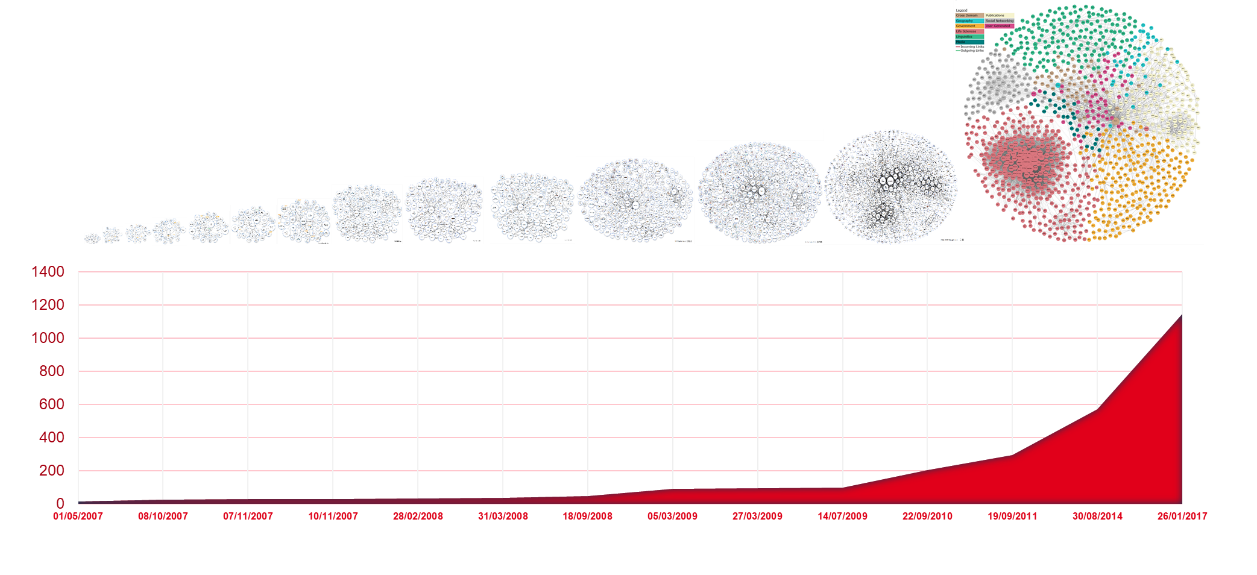
\includegraphics[width=5.0in]{media/image1.png}
    \caption{number of linked open datasets on the Web in the linked open
data cloud}
    \label{fig:ch1.1}
\end{figure}


\subsubsection{What about the round-worlders?}

The network effect has already proven to be an effective and empowering
way to muster the effort needed to create a massive information network
like the World Wide Web; in fact, it is the only method that has
actually succeeded in creating such a structure. The AAA slogan enables
the network effect that made the rapid growth of the Web possible. But
what are some of the ramifications of such an open system? What does the
AAA slogan imply for the content of an organically grown web?

For the network effect to take hold, we have to be prepared to cope with
a wide range of variance in the information on the Web. Sometimes the
differences will be minor details in an otherwise agreed-on area; at
other times, differences may be essential disagreements that drive
political and cultural discourse in our society. This phenomenon is
apparent in the hypertext web today; for just about any topic, it is
possible to find web pages that express widely differing opinions about
that topic. The ability to disagree, and at various levels, is an
essential part of human discourse and a key aspect of the Web that makes
it successful. Some people might want to put forth a very odd opinion on
any topic; someone might even want to postulate that the world is round,
while others insist that it is flat. The infrastructure of the Web must
allow both of these (contradictory) opinions to have equal availability
and access.

There are a number of ways in which two speakers on the Web may
disagree. We will illustrate each of them with the example of the status
of Pluto as a planet:


\begin{itemize}
\item
  \emph{They may fundamentally disagree on some topic}. While the IAU
  has changed its definition of planet in such a way that Pluto is no
  longer included, it is not necessarily the case that every astronomy
  club or even national body agrees with this categorization. Many
  astrologers, in particular, who have a vested interest in considering
  Pluto to be a planet, have decided to continue to consider Pluto as a
  planet. In such cases, different sources will simply disagree.
\item
  \emph{Someone might want to intentionally deceive}. Someone who
  markets posters, models, or other works that depict nine planets has a
  good reason to delay reporting the result from the IAU and even to
  spreading uncertainty about the state of affairs.
\item
  \emph{Someone might simply be mistaken}. Web sites are built and
  maintained by human beings, and thus they are subject to human error.
  Some web site might erroneously list Pluto as a planet or, indeed,
  might even erroneously fail to list one of the eight ``nondwarf''
  planets as a planet.
\item
  \emph{Some information may be out of date}. There are a number of
  displays around the world of scale models of the solar system, in
  which the status of the planets is literally carved in stone; these
  will continue to list Pluto as a planet until such time as there is
  funding to carve a new description for the ninth object. Web sites are
  not carved in stone, but it does take effort to update them; not
  everyone will rush to accomplish this.
\end{itemize}


While some of the reasons for disagreement might be, well, disagreeable
(wouldn't it be nice if we could stop people from lying?), in practice
there isn't any way to tell them apart. The infrastructure of the Web
has to be able to cope with the fact that information on the Web will
disagree from time to time and that this is not a temporary condition.
It is in the very nature of the Web that there be variations and
disagreement.

The Semantic Web is often mistaken for an effort to make everyone agree
on a single ontology--- but that just isn't the way the Web works. The
Semantic Web isn't about getting everyone to agree, but rather about
coping in a world where not everyone will agree and achieving some
degree of interoperability anyway. In the data themselves too we may
find disagreement; for instance the numbers of casualties in a conflict
may be reported on the Web of data with very different values from the
involved parties. There will always be multiple ontologies and diverging
statements, just as there will always be multiple web pages on any given
topic. The Web is innovative because it allows all these multiple
viewpoints to coexist.

\subsubsection{To each their own}

How can the Web architecture support this sort of variation of opinion?
That is, how can two people say different things, about the same topic?
There are two approaches to this issue. First, we have to talk a bit
about how one can make any statement at all in a web context.

The IAU can make a statement in plain English about Pluto, such as
``Pluto is a dwarf planet,'' but such a statement is fraught with all
the ambiguities and contextual dependencies inherent in natural
language. We think we know what ``Pluto'' refers to, but how about
``dwarf planet''? Is there any possibility that someone might disagree
on what a ``dwarf planet'' is? How can we even discuss such things?

The first requirement for making statements on a global web is to have a
global way of identifying the entities we are talking about. We need to
be able to refer to ``the notion of Pluto as used by the IAU'' and ``the
notion of Pluto as used by the American Federation of Astrologers'' if
we even want to be able to discuss whether the two organizations are
referring to the same thing by these names.

In addition to Pluto, another object was also classified as a ``dwarf
planet.'' This object is sometimes known as UB313 and sometimes known by
the name Xena. How can we say that the object known to the IAU as UB313
is the same object that its discoverer Michael Brown calls ``Xena''?

One way to do this would be to have a global arbiter of names decide how
to refer to the object. Then Brown and the IAU can both refer to that
``official'' name and say that they use a private ``nickname'' for it.
Of course, the IAU itself is a good candidate for such a body, but the
process to name the object took over two years. Coming up with good,
agreed-on global names is not always easy business.

On the Web we name things with URIs (Uniform Resource Identifier). The
URI standard provides rules to mint identifiers for anything around us.
The most common form of URIs are the URLs (Uniform Resource Locator)
commonly called Web addresses (e.g. http://www.inria.fr/) that locate a
specific resource on the Web. In the absence of an agreement, different
Web authors will select different URIs for the same real-world resource.
Brown's \emph{Xena} is IAU's \emph{UB313}. When information from these
different sources is brought together in the distributed network of
data, the Web infrastructure has no way of knowing that these need to be
treated as the same entity. The flip side of this is that we cannot
assume that just because two URIs are distinct, they refer to distinct
resources. This feature of the Semantic Web is called the Non-unique
Naming Assumption; that is, we have to assume (until told otherwise)
that some Web resource might be referred to using different names by
different people. It's also crucial to note that there are times when
unique names might be nice, but it may be impossible. Some other
organization than the IAU, for example, might decide they are unwilling
to accept the new nomenclature.

\subsubsection{There's always one more}
\label{openworld}

In a distributed network of information, as a rule we cannot assume at
any time that we have seen all the information in the network, or even
that we know everything that has been asserted about one single topic.
This is evident in the history of Pluto and UB313. For many years, it
was sufficient to say that a planet was defined as ``any object of a
particular size orbiting the sun.'' Given the information available
during that time, it was easy to say that there were nine planets around
the sun. But the new information about UB313 changed that; if a planet
is defined to be any body that orbits the sun of a particular size, then
UB313 had to be considered a planet, too. Careful speakers in the late
twentieth century, of course, spoke of the ``known'' planets, since they
were aware that another planet was not only possible but even suspected
(the so-called ``Planet X,'' which stood in for the unknown but
suspected planet for many years).

The same situation holds for the Semantic Web. Not only might new
information be discovered at any time (as is the case in solar system
astronomy), but, because of the networked nature of the Web, at any one
time a particular server that holds some unique information might be
unavailable. For this reason, on the Semantic Web we can rarely conclude
things like ``there are nine planets,'' since we don't know what new
information might come to light.

In general, this aspect of a Web has a subtle but profound impact on how
we draw conclusions from the information we have. It forces us to
consider the Web as an Open World and to treat it using the Open World
Assumption. An Open World in this sense is one in which we must assume
at any time that new information could come to light, and we may draw no
conclusions that rely on assuming that the information available at any
one point is all the information available.

For many applications, the Open World Assumption makes no difference; if
we draw a map of all the Mongotel hotels in Boston, we get a map of all
the ones we know of at the time. The fact that Mongotel might have more
hotels in Boston (or might open a new one) does not invalidate the fact
that it has the ones it already lists. In fact, for a great deal of
Semantic Web applications, we can ignore the Open World Assumption and
simply understand that a semantic application, like any other web page,
is simply reporting on the information it was able to access at one
time.

The openness of the Web only becomes an issue when we want to draw
conclusions based on distributed data. If we want to place Boston in the
list of cities that are not served by Mongotel (e.g., as part of a
market study of new places to target Mongotels), then we cannot assume
that just because we haven't found a Mongotel listing in Boston, no such
hotel exists.

As we shall see in the following chapters, the Semantic Web includes
features that correspond to all the ways of working with Open Worlds
that we have seen in the real world. We can draw conclusions about
missing Mongotels if we say that some list is a comprehensive list of
all Mongotels. We can have an anonymous ``Planet X'' stand in for an
unknown but anticipated entity. These techniques allow us to cope with
the Open World Assumption in the Semantic Web, just as they do in the
Open World of human knowledge.

In contrast to the Open World Assumption, most data systems operate under the
\emph{Closed World Assumption}, that is, if we are missing some data in a document or a record,
then that data is simply not available.  In many situations (such as when evaluating
documents that have a set format or records that conform to a particular data base schema),
the Closed World Assumption is appropriate.   The Semantic Web standards have provisions for
working with the Closed World Assumption when it is appropriate. 


\subsubsection{The nonunique name of the semantic Web}

One problem the first time you discover linked data on the Web and
semantic Web is that this evolution of the Web is perceived and
presented under different names, each name insisting on a different
facet of the overall architecture of this evolution. In the title of
this book, we refer to the Semantic Web, emphasizing the importance of
meaning to data sharing. The Semantic Web is known by many other names.
The name ``Web of data'' refers to the opportunity now available on the
Web to open silos of data of all sizes, from the small dataset of a
personal hotel list up to immense astronomic databases, and to exchange,
connect and combine them on the Web according to our needs. The name
``linked data'' refers to the fact we can use the Web addressing and
linking capabilities to link data pieces inside and between datasets
across the Web much in the same way we reference and link Web pages on
the hypertext Web. Only this time, because we are dealing with structured
data, applications can process these data and follow the links to
discover new data in many more automated ways. The name ``linked open
data'' focuses on the opportunity to exploit open data from the Web in
our applications and the high benefit there is in using and reusing URIs
to join assertions from different sources. This name also reminds us
that linked data are not necessarily open and that all the techniques we
are introducing here can also be used in private spaces (intranets,
intrawebs, extranets, etc.). In an enterprise, we often refer to a
``Knowledge Graph'', which is specific to that enterprise, but can
include any information that the enterprise needs to track (including
information about other enterprises that it does business with). The
name ``giant global graph'' puts into perspective the billions of links
between data distributed on the Web and which, joined through URIs,
produce a giant graph. The name ``semantic web'' emphasizes the ability
we now have for exchanging our data models, schemas, vocabularies, in
addition to datasets, and the associated semantics in order to enrich
the range of automatic processing that can be performed on them as we
will see in Chapter 7.

\section{SUMMARY}

The aspects of the Web we have outlined here---the AAA slogan, the
network effect, nonunique naming, and the Open World
Assumption---already hold for the hypertext Web. As a result, the Web
today is something of an unruly place, with a wide variety of different
sources, organizations, and styles of information. Effective and
creative use of search engines is something of a craft; efforts to make
order from this include community efforts like social bookmarking and
community encyclopedias to automated methods like statistical
correlations and fuzzy similarity matches.

For the Semantic Web, which operates at the finer level of individual
statements about data, the situation is even wilder. With a human in the
loop, contradictions and inconsistencies in the hypertext Web can be
dealt with by the process of human observation and application of common
sense. With a machine combining information, how do we bring any order
to the chaos? How can one have any confidence in the information we
merge from multiple sources? If the hypertext Web is unruly, then surely
the Semantic Web is a jungle---a rich mass of interconnected
information, without any road map, index, or guidance.

How can such a mess become something useful? That is the challenge that
faces the working ontologist. Their medium is the distributed web of
data; their tools are the Semantic Web languages RDF, RDFS, SPARQL,
SKOS, SHACL and OWL. Their craft is to make sensible, usable, and
durable information resources from this medium. We call that craft
modeling, and it is the centerpiece of this book.

The cover of this book shows a system of channels with water coursing
through them. If we think of the water as the data on the Web, the
channels are the model. If not for the model, the water would not flow
in any systematic way; there would simply be a vast, undistinguished
expanse of water. Without the water, the channels would have no
dynamism; they have no moving parts in and of themselves. Put the two
together, and we have a dynamic system. The water flows in an orderly
fashion, defined by the structure of the channels. This is the role that
a model plays in the Semantic Web.

Without the model, there is an undifferentiated mass of data; there is
no way to tell which data can or should interact with other data. The
model itself has no significance without data to describe it. Put the
two together, however, and you have a dynamic web of information, where
data flow from one point to another in a principled, systematic fashion.
This is the vision of the Semantic Web---an organized worldwide system
where information flows from one place to another in a smooth but
orderly way.

\subsection{Fundamental concepts}

The following fundamental concepts were introduced in this chapter.

\textbf{The AAA slogan}---Anyone can say Anything about Any topic. One
of the basic tenets of the Web in general and the Semantic Web in
particular.

\textbf{Open world/Closed world}---A consequence of the AAA slogan is
that there could always be something new that someone will say; this
means that we must assume that there is always more information that
could be known.

\textbf{Nonunique naming}---Since the speakers on the Web won't
necessarily coordinate their naming efforts, the same entity could be
known by more than one name.

\textbf{The network effect}---The property of a web that makes it grow
organically. The value of joining in increases with the number of people
who have joined, resulting in a virtuous cycle of participation.

\textbf{The data wilderness}---The condition of most data on the web. It
contains valuable information, but there is no guarantee that it will be
orderly or readily understandable.



        % Chapter 1.
\chapter{Semantic Modeling}
What would you call a world in which any number of people can speak,
when you never know who has something useful to say, and when someone
new might come along at any time and make a valuable but unexpected
contribution? What if just about everyone had the same goal of advancing
the collaborative state of knowledge of the group, but there was little
agreement (at first, anyway) about how to achieve it?

If your answer is ``That sounds like the Web and Semantic Web!'', you
are right (and you must have read Chapter~\ref{ch1}). If your answer is ``It
sounds like any large group trying to understand a complex phenomenon,''
you are even more right. The jungle that is the Semantic Web is not a
new thing; this sort of chaos has existed since people first tried to
make sense of the world around them.

What intellectual tools have been successful in helping people sort
through this sort of tangle? Any number of analytical tools has been
developed over the years, but they all have one thing in common: They
help people understand their world by forming an abstract description
that hides certain details while illuminating others. These abstractions
are called models, and they can take many forms.

How do models help people assemble their knowledge? Models assist in
three essential ways:


\begin{enumerate}
\def\labelenumi{\arabic{enumi}.}
\item
  \emph{Models help people communicate}. A model describes the situation
  in a particular way that other people can understand.
\item
  \emph{Models explain and make predictions}. A model relates primitive
  phenomena to one another and to more complex phenomena, providing
  explanations and predictions about the world.
\item
  \emph{Models mediate among multiple viewpoints}. No two people agree
  completely on what they want to know about a phenomenon; models
  represent their commonalities while allowing them to explore their
  differences.
\end{enumerate}

The Semantic Web standards have been created not only as a medium in
which people can collaborate by sharing information but also as a medium
in which people can collaborate on models. Models that they can use to
organize the information that they share. Models that they can use to
advance the common collection of knowledge.

How can a model help us find our way through the mess that is the Web?
How do these three features help? The first feature, human
communication, allows people to collaborate on their understanding. If
someone else has faced the same challenge that you face today, perhaps
you can learn from their experience and apply it to yours. There are a
number of examples of this in the Web today, of newsgroups, mailing
lists, forums, social medias and wikis where people can ask questions
and get answers. In the case in which the information needs are fairly
uniform, it is not uncommon for a community or a company to assemble a
set of ``Frequently Asked Questions,'' or FAQs, that gather the
appropriate knowledge as answers to these questions. As the number of
questions becomes unmanageable, it is not uncommon to group them by
topic, by task, by affected subsystem, and so forth. This sort of
activity, by which information is organized for the purpose of sharing,
is the simplest and most common kind of modeling, with the sole aim of
helping a group of people collaborate in their effort to sort through a
complex set of knowledge.

The second feature, explanation and prediction, helps individuals make
their own judgments based on information they receive. FAQs are useful
when there is a single authority that can give clear answers to a
question, as is the case for technical assistance for using some
appliance or service. But in more interpretive situations, someone might
want or need to draw a conclusion for themselves. In such a situation, a
simple answer as given in a FAQ is not sufficient. Politics is a common
example from everyday life. Politicians in debate do not tell people how
to vote, but they try to convince them to vote in one way or another.
Part of that convincing is done by explaining their position and
allowing the individual to evaluate whether that explanation holds true
to their own beliefs about the world. They also typically make
predictions: If we follow this course of action, then a particular
outcome will follow. Of course, a lot more goes into political
persuasion than the argument, but explanation and prediction are key
elements of a persuasive argument.

Finally, the third feature, mediation of multiple viewpoints, is
essential to fostering understanding in a web environment. As the web of
opinions and facts grows, many people will say things that disagree
slightly or even outright contradict what others are saying. Anyone who
wants to make their way through this will have to be able to sort out
different opinions, representing what they have in common as well as the
ways in which they differ. This is one of the most essential organizing
principles of a large, heterogeneous knowledge set, and it is one of the
major contributions that modeling makes to helping people organize what
they know.

Astrologers and the IAU agree on the planethood of Mercury, Venus,
Earth, Mars, Jupiter, Saturn,
Uranus, and Neptune. The IAU also agrees with astrologers that Pluto is
a planet, but it disagrees by calling it a dwarf planet. Astrologers (or
classical astronomers) do not accept the concept of dwarf planets, so
they are not in agreement with the IAU, which categorizes UB313 and
Ceres as such. A model for the Semantic Web must be able to organize
this sort of variation, and much more, in a meaningful and manageable
way.

\section{Modeling for Human Communication}

Models used for human communication have a great advantage over models
that are intended for use by computers; they can take advantage of the
human capacity to interpret signs to give them meaning. This means that
communication models can be written in a wide variety of forms,
including plain language or ad hoc images. A model can be explained by
one person, amended by another, interpreted
by a third person, and so on. Models written in natural language have
been used in all manner of intellectual life, including science,
religion, government, and mathematics.

But this advantage is a double-edged sword; when we leave it to humans
to interpret the meaning of a model, we open the door for all manner of
abuse, both intentional and unintentional. Legislation provides a good
example of this. A governing body like a parliament or a legislature
enacts laws that are intended to mediate rights and responsibilities
between various parties. Legislation typically sets up some sort of
model of a situation, perhaps involving money (e.g., interest caps,
taxes); access rights (who can view what information, how can
information be legally protected); personal freedom (how freely can one
travel across borders, when does the government have the right to
restrict a person's movements); or even the structure of government
itself (who can vote and how are those votes counted, how can government
officials be removed from office). These models are painstakingly
written in natural language and agreed on through an elaborate process
(which is also typically modeled in natural language).

It is well known to anyone with even a passing interest in politics that
good legislation is not an easy task and that crafting the words
carefully for a law or statute is very important. The same flexibility
of interpretation that makes natural language models so flexible also
makes it difficult to control how the laws will be interpreted in the
future. When someone else reads the text, they will have their own
background and their own interests that will influence how they
interpret any particular model. Readers of the previous paragraph in the
third edition probably interpreted it very differently from readers of
the first edition only a decade earlier, despite the fact that the text
has not changed at all. This phenomenon is so widespread that most
government systems include a process (usually involving a court
magistrate and possibly a committee of citizens) whereby disputes over
the interpretation of a law or its applicability can be resolved.

When a model relies on particulars of the context of its reader for
interpretation of its meaning, as is the case in legislation, we say
that a model is \emph{informal}. That is, the model lacks a formalism
whereby the meaning of terms in the model can be uniquely defined.

In the hypertext web today, there are informal models that help people
communicate about the organization of the information. It is common for
commerce web sites to organize their wares in catalogs with category
names like ``web-cams,'' ``Oxford shirts,'' and ``Granola.'' In such
cases, the communication is primarily one way; the catalogue designer
wants to communicate to the buyers the information that will help them
find what they want to buy. The interpretation of these words is up to
the buyers. The effectiveness of such a model is measured by the degree
to which this is successful. If enough people interpret the categories
in a way similar enough to the intent of the cataloguer, then they will
find what they want to buy. There will be the occasional discrepancy
like ``Why wasn't that item listed as a \emph{webcam}?'' or ``That's not
granola, that's just plain cereal!'' But as long as the interpretation
is close enough, the model is successful.

A more collaborative style of document modeling comes in the form of
community tagging. A number of web sites have been successful by
allowing users to provide meaningful symbolic descriptions of their
content in the form of \emph{tags}. A tag in this sense is simply a
single word or short phrase that describes some aspect of the content.
Early examples of this sort of tagging system include Flickr for photos
and del.icio.us for Web bookmarks. In more modern systems, we see
``hashtags'' in social media like Twitter, LinkedIn and Facebook playing
a similar role. Users of content organization services like Slideshare
for presentations and YouTube for videos use tags to help other users
find and discover content. The idea of community tagging is that each
individual who provides content will describe it using tags of their own
choosing. If any two people use the same tag, this becomes a common
organizing entity; anyone who is browsing for content can access
information from both contributors under that tag. The tagging
infrastructure shows which tags have been used by many people. Not only
does this help browsers determine what tags to use in a search, but it
also helps content providers to find commonly used tags that they might
want to use to describe new content. Thus, a tagging system will have a
certain self-organizing character, whereby popular tags become more
popular and unpopular tags remain unpopular---something like evolution
by artificial selection of tags. The resulting collection of tags and
their relations is called a \emph{Folksonomy} to reflect the fact this
is a categorization from and by the crowd.

Tagging systems of this sort provide an informal organization to a large
body of heterogeneous information. The organization is informal in the
sense that the interpretation of the tags requires human processing in
the context of the consumer. Just because a tag is popular doesn't mean
that everyone is using it in the same way. In fact, the community
selection process actually selects tags that are used in several
different ways, whether they are compatible or not. As more and more
people provide content, the popular tags saturate with a wide variety of
content, making them less and less useful as discriminators for people
browsing for content. This sort of problem is inherent in information
modeling systems; since there isn't an objective description of the
meaning of a symbol outside the context of the provider and consumer of
the symbol, the communication power of that symbol degrades as it is
used in more and more contexts.

When tags are used incompatibly, it is a challenge to both humans and machines to differentiate there meaning.  For example, the twitter hashtag ``\#rpi'' is currently used for a university in the US, a British currency concept, the Spanish term for someone who has passed away, and a shorthand for the Raspberry Pi computer. 
While these would seem very different, when coupled with technology like search engines or social networks, the term becomes a challenge to differentiate - a tweet like
``\#rpi is up'' could refer to the university leading in a sports event, the British economy doing well, or someone having attached the small computer to a tree in their backyard (Lest you think this is far-fetched,  this was a real tweet which was indeed about someone putting their Raspberry Pi into a tree-house).

Formality of a model isn't a black-and-white judgment; there can be
degrees of formality. This is clear in legal systems, where it is common
to have several layers of legislation, each one giving objective context
for the next. A contract between two parties is usually governed by some
regional law that provides standard definitions for terms in the
contract. Regional laws are governed by national laws, which provide
constraints and definitions for their terms. National laws have their
own structure, in which a constitution or a body of case law provides a
framework for new decisions and legislation. Even though all these
models are expressed in natural language and fall back on human
interpretation in the long run, they can be more formal than private
agreements that rely almost entirely on the interpretation of the
agreeing parties.

This layering of informal models sometimes results in a modeling style
that is reminiscent of Talmudic scholarship. The content of the Talmud
includes not only the original scripture but also interpretative
comments on the scripture by authoritative sources (classical rabbis).
Their comments have gained such respect that they are traditionally
published along with the original scripture for comment by later rabbis,
whose comments in turn have become part of the intellectual tradition.
The original scripture, along with all the authoritative comments, is
collectively called the Talmud, and it is the basis of a classical
Jewish education to this day.

A similar effect happens with informal models. The original model is
appropriate in some context, but as its use expands beyond that context,
further models are required to provide common context to explicate the
shared meaning. But if this further exposition is also informal, then
there is the risk that its meaning will not be clear, so further
modeling must be done to clarify that. This results in heavily layered
models, in which the meaning of the terms is always subject to further
interpretation. It is the inherent ambiguity of natural language at each
level that makes the next layer of commentary necessary until the degree
of ambiguity is ``good enough'' that no more levels are needed. When it
is possible to choose words that are evocative and have considerable
agreement, this process converges much more quickly.

Human communication, as a goal for modeling, allows it to play a role in
the ongoing collection of human knowledge. The levels of communication
can be quite sophisticated, including the collection of information used
to interpret other information. In this sense, human communication is
the fundamental requirement for building a Semantic Web. It allows
people to contribute to a growing body of knowledge and then draw from
it. But communication is not enough; to empower a web of human
knowledge, the information in a model needs to be organized in such a
way that it can be useful to a wide range of consumers.

\section{Explanation and Prediction}

Models are used to organize human thought in the form of explanations.
When we understand how a phenomenon results from other basic principles,
we gain a number of advantages. Not least is the feeling of confidence
that we have actually understood it; people often claim to ``have a
grasp on'' or ``have their head around'' an idea when they finally
understand it. Explanation plays a major role in this sort of
understanding. Explanation also assists in memory; it is easier to
remember that putting a lid on a flaming pot can quench the flame if one
knows the explanation that fire requires air to burn. Most important for
the context of the Semantic Web, explanation makes it easier to reuse a
model in whole or in part; an explanation relates a conclusion to more
basic principles. Understanding how a pot lid quenches a fire can help
one understand how a candle snuffer works. Interpretability and
explanation are vital for establishing trust in a model and to
effectively support decision making. You are more likely to trust my
model, if I can provide results you can interpret and explanations so
that you can understand why the model is appropriate. Interpretability
and explanation are the keys to understanding when a model is applicable
and when it is not.

Closely related to this aspect of a model is the idea of prediction.
When a model provides an adequate explanation of a phenomenon, it can
also be used to make predictions. This aspect of models is what makes
their use central to the scientific method, where falsification of
predictions made by models forms the basis of the methodology of
inquiry.

Explanation and prediction typically require models with a good deal
more formality than is usually required for human communication. An
explanation relates a phenomenon to ``first principles''; these
principles, and the rules by which they are related, do not depend on
interpretation by the consumer but instead are in some objective form
that stands outside the communication. Such an objective form, and the
rules that govern how it works, is called a formalism.

Formal models are the bread and butter of mathematical modeling, in
which very specific rules for calculation and symbol manipulation govern
the structure of a mathematical model and the valid ways in which one
item can refer to another. Explanations come in the form of proofs, in
which steps from premises (stated in some formalism) to conclusions are
made according to strict rules of transformation for the formalism.
Formal models are used in many human intellectual endeavors, wherever
precision and objectivity are required.

Formalisms can also be used for predictions. Given a description of a
situation in some formalism, the same rules that govern transformations
in proofs can be used to make predictions. We can explain the trajectory
of an object thrown out of a window with a formal model of force,
gravity, speed, and mass, but given the initial conditions of the object
thrown, we can also compute, and thus predict, its trajectory.

Formal prediction and explanation allow us to evaluate when a model is
applicable. Furthermore, the formalism allows that evaluation to be
independent of the listener. One can dispute the result that 
$2 + 2 = 4$ by questioning just what the terms $2$, $4$, $+$, and
$=$ mean, but once people agree on what they mean, they cannot
(reasonably) dispute that this formula is correct.

Formal modeling therefore has a very different social dynamic than
informal modeling; because there is an objective reference to the model
(the formalism), there is no need for the layers of interpretation that
result in Talmudic modeling. Instead of layers and layers of
interpretation, the buck stops at the formalism.

As we shall see, the Semantic Web standards include a small variety of
modeling formalisms. Because they are formalisms, modeling in the
Semantic Web need not become a process of layering interpretation on
interpretation. Also, because they are formalisms, it is possible to
couch explanations in the Semantic
Web in the form of proofs and to use that proof mechanism to make
predictions. This aspect of Semantic
Web models goes by the name \emph{inference} and it will be discussed in
detail in Chapter~\ref{ch7}.

\section{Mediating Variability}

In any Web setting, variability is to be expected and even embraced. The
dynamics of the network effect require the ability to represent a
variety of opinions. A good model organizes those opinions so that the
things that are common can be represented together, while the things
that are distinct can be represented as well.

Let's take the case of Pluto as an example. From 1930 until 2006, it was
considered to be a planet by astronomers and astrologers alike. After
the redefinition of planet by the IAU in 2006, Pluto was no longer
considered to be a planet but more specifically a dwarf planet by the
IAU and by astronomers who accept the IAU as an authority. Astrologers,
however, chose not to adopt the IAU convention, and they continued to
consider Pluto a planet. Some amateur astronomers, mostly for nostalgic
reasons, also continued to consider Pluto a planet. How can we
accommodate all of these variations of opinion on the Web?

One way to accommodate them would be to make a decision as to which one
is ``preferred'' and to control the Web so that only that position is
supported. This is the solution that is most commonly used in corporate
data centers, where a small group or even a single person acts as the
database administrator and decides what data are allowed to live in the
corporate database. This solution is not appropriate for the Web because
it does not allow for the AAA slogan (see Chapter 1) that leads to the
network effect.

Another way to accommodate these different viewpoints would be to simply
allow each one to be represented separately, with no reference to one
another at all. It would be the responsibility of the information
consumer to understand how these things relate to one another and to
make any connections as appropriate. This is the basis of an informal
approach, and it indeed describes the state of the hypertext web as it is
today. A Web search for Pluto will turn up a wide array of articles, in
which some call it a planet (e.g., astrological ones or astronomical
ones that have not been updated), some call it a dwarf planet (IAU
official web sites), and some that are still debating the issue. The
only way a reader can come to understand what is common among these
things---the notion of a planet, of the solar system, or even of Pluto
itself---is through reader interpretation.

How can a model help sort this out? How can a model describe what is
common about the astrological notion of a planet, the twentieth-century
astronomical notion of a planet, and the post-2006 notion of a planet?
The model must include an identification mechanism (e.g. URI) to
separate the naming from description and it must also allow for each of
the differing viewpoints to be expressed.

\subsection{Variation and classes}

This problem is not a new one; it is a well-known problem in software
engineering. When a software component is designed, it has to provide
certain functionality, determined by information given to it at runtime.
There is a trade-off in such a design; the component can be made to
operate in a wide variety of circumstances, but it will require a
complex input to describe just how it should behave at any one time. Or
the system could be designed to work with very simple input but be
useful in only a small number of very specific situations. The design of
a software component inherently involves a model of the commonality and
variability in the environment in which it is expected to be deployed.
In response
to this challenge, software methodology has developed the art of object
modeling (in the context of Object-Oriented Programming, or OOP) as a
means of organizing commonality and variability in software components.

One of the primary organizing tools in OOP is the notion of a hierarchy
of classes and subclasses. Classes high up in the hierarchy represent
functionality that is common to a large number of components; classes
farther down in a hierarchy represent more specific functionality.
Commonality and variability in the functionality of a set of software
components is represented in a class hierarchy.

The Semantic Web standards also use this idea of class hierarchy for
representing commonality and variability. Since the Semantic Web, unlike
OOP, is not focused on software representation, classes are not defined
in terms of behaviors of functions. But the notion of classes and
subclasses remains, and it plays much the same role. High-level classes
represent commonality among a large variety of entities, whereas
lower-level classes represent commonality among a small, specific set of
things.

Let's take Pluto as an example. The 2006 IAU definition of planet is
quite specific in requiring these three criteria for a celestial body to
be considered a planet:

1. It is in orbit around the sun.

2. It has sufficient mass to be nearly round.

3. It has cleared the neighborhood around its orbit.

The IAU goes further to state that a dwarf planet is a body that
satisfies conditions 1 and 2 (and not 3); a body that satisfies only
condition 1 is a small solar system body (SSSB). These definitions make
a number of things clear: The classes SSSB, dwarf planet, and planet are
all mutually exclusive; no celestial body is a member of any two
classes. However, there is something that all of them have in common:
They all are in orbit around the sun.

Twentieth-century astronomy and astrology are not quite as organized as
this; they don't have such rigorous definitions of the word
\emph{planet}. So how can we relate these notions to the
twenty-first-century notion of \emph{planet}?

The first thing we need is a way to talk about the various uses of the
word \emph{planet}: the IAU use, the astrological use, and the
twentieth-century astronomical use. This seems like a simple
requirement, but until it is met, we can't even talk about the
relationship among these terms. We will see details of the Semantic Web
solution to this issue in Chapter 3, but for now, we will simply prefix
each term with a short abbreviation of its source---for example, use
IAU:Planet for the IAU use of the word, horo:Planet for the astrological
use, and astro:Planet for the twentieth-century astronomical use.

The solution begins by noticing what it is that all three notions of
planet have in common; in this case, it is that the body orbits the sun.
Thus, we can define a class of the things that orbit the sun, which we
may as well call solar system body, or SSB for short. All three notions
are subclasses of this notion. This can be depicted graphically as in
Figure~\ref{fig:ch2.1}.

We can go further in this modeling when we observe that there are only
eight IAU:Planets, and each one is also a horo:Planet and an
astro:Planet. Thus, we can say that IAU:Planet is a subclass of both
horo:Planet and astro:Planet, as shown in Figure~\ref{fig:ch2.2}. We can continue in
this way, describing the relationships among all the concepts we have
mentioned so far: IAU:DwarfPlanet and IAU:SSSB. As we go down the tree,
each class refers to a more restrictive set of entities. In this way, we
can model the commonality among entities (at the high level) while
respecting their variation (at a low level).


\begin{figure}
    \centering
    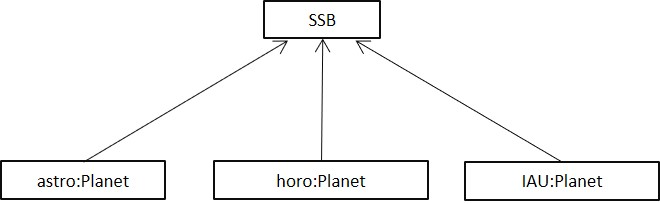
\includegraphics[width=5.0in]{SWWOv3/media/ch2/f02-01.jpg}
    \caption{Subclass diagram for different notions of planet.}
    \label{fig:ch2.1}
\end{figure}


\begin{figure}
    \centering
    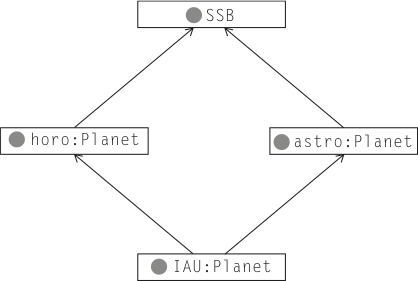
\includegraphics[width=5.0in]{SWWOv3/media/ch2/f02-02.jpg}
    \caption{More detailed relationships between various notions of planet.}
    \label{fig:ch2.2}
\end{figure}


\subsection{Variation and layers}

Classes and subclasses are a fine way to organize variation when there
is a simple, known relationship between the modeled entities and it is
possible to determine a clear ordering of classes that describes these
relationships. In a Web setting, however, this usually is not the case.
Each contributor can have something new to say that may fit in with
previous statements in a wide variety of ways. How can we accommodate
variation of sources if we can't structure the entities they are
describing into a class model?

The Semantic Web provides an elegant solution to this problem. The basic
idea is that any model can be built up from contributions from multiple
sources. One way of thinking about this is to consider a model to be
described in layers. Each layer comes from a different source. The
entire model is the combination of all the layers, viewed as a single,
unified whole.

Let's have a look at how this could work in the case of Pluto. Figure~\ref{fig:ch2.3} 
illustrates how different communities could assert varying
information about Pluto. In part (a) of the figure, we see some
information about Pluto that is common among astrologers---namely, that
Pluto signifies rebirth and regeneration and that the preferred symbol
for referring to Pluto is the glyph indicated. Part (b) shows some
information that is of concern to astronomers, including the composition
of the body Pluto and their preferred symbol. How can this variation be
accommodated in a web of information? The simplest way is to simply
merge the two models into a single one that includes all the information
from each model, as shown in part (c).

\begin{figure}
    \centering
    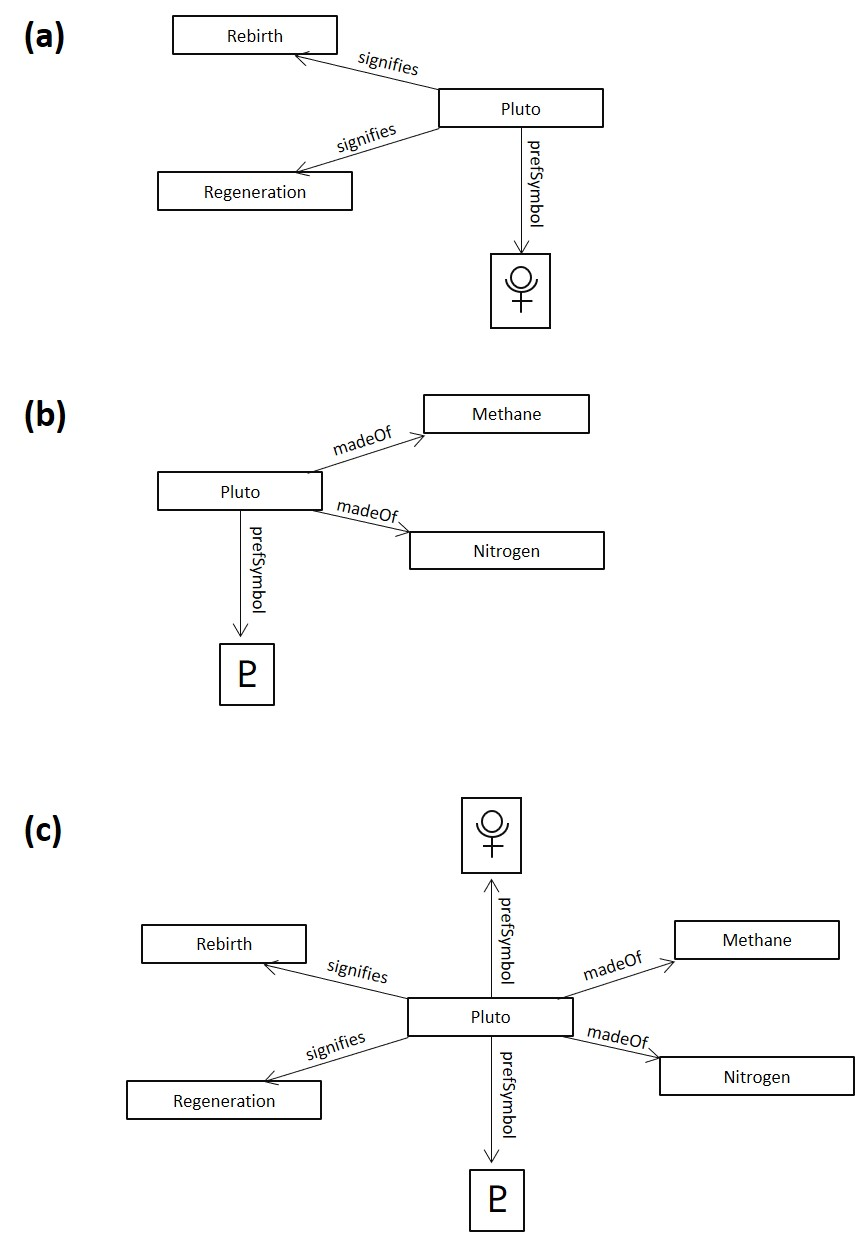
\includegraphics[width=5.0in]{SWWOv3/media/ch2/f02-03abc.jpg}
    \caption{Layers of modeled information about Pluto.}
    \label{fig:ch2.3}
\end{figure}

Merging models in this way is a conceptually simple thing to do, but how
does it cope with variability? In the first place, it copes in the
simplest way possible: It allows the astrologers and the astronomers to
both have their say about Pluto (remember the AAA slogan!). For any
party that is interested in both of these things (perhaps someone
looking for a spiritual significance for elements?), the information can
be viewed as a single, unified whole.

But merging models in this way has a drawback as well. In Figure~\ref{fig:ch2.3}(c),
there are two distinct glyphs, each claiming to be the ``preferred''
symbol for Pluto. This brings up issues of consistency of viewpoints. On
the face of it, this appears to be an inconsistency because, from its
name, we might expect that there can be exactly one preferred symbol
(prefSymbol) for any solar system body. But how can a machine know that?
For a machine, the name prefSymbol can't be treated any differently from
any other label---for instance, madeOf or signifies. In such a context,
how can we even tell that this is an inconsistency? After all, we don't
think it is an inconsistency that Pluto can be composed of more than one
chemical compound or that it can signify more than one spiritual theme.
Do we have to describe this in a natural language commentary on the
model?

Detailed answers to questions like these are exactly the reason why we
need to publish models on the Semantic Web. When two (or more!)
viewpoints come together in a web of knowledge, there will typically be
overlap, disagreement, and confusion before there is synergy,
cooperation, and collaboration. If the infrastructure of the Web is to
help us to find our way through the wild stage of information sharing,
an informal notion of how things fit together, or should fit together,
will not suffice. It is easy enough to say that we have an intuition
that states there is something special about \texttt{prefSymbol} that makes it
different from \texttt{madeOf} or \texttt{signifies}. If we can inform our 
infrastructure about this distinction in a sufficiently formal way, then it
can, for instance, detect discrepancies of this sort and, in some cases,
even resolve them.

This is the essence of modeling in the Semantic Web: providing an
infrastructure where not only can anyone say anything about any topic
but the infrastructure can help a community work through the resulting
chaos. A model can provide a framework (like classes and subclasses) for
representing and organizing commonality and variability of viewpoints
when they are known. But in advance of such an organization, a model can
provide a framework for describing what sorts of things we can say about
something. We might not agree on the symbol for Pluto, but we can agree
that it should have just one preferred symbol.

\section{Expressivity in Modeling}

There is a trade-off when we model, and although anyone can say anything
about any topic, not everyone will want to say certain things. There are
those who are interested in saying details about individual entities,
like the preferred symbol for Pluto or the themes in life that it
signifies. Others (like that IAU) are interested in talking about
categories, what belongs in a category, and how you can tell the
difference. Still others (like lexicographers, information architects,
and librarians) want to talk about the rules for specifying information,
such as whether there can be more than one preferred label for any
entity. All of these people have contributions to make to the web of
knowledge, but the kinds of contributions they make are very different,
and they need different tools. This difference is one of \emph{level of
expressivity}.



\begin{figure}
    \centering
    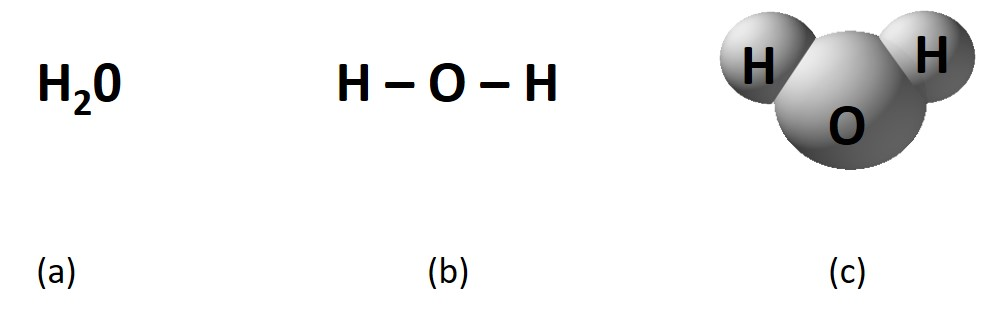
\includegraphics[width=5.0in]{media/ch2/figure-02-04.jpg}
    \caption{Different expressivity of models of a water molecule.}
    \label{fig:ch2.4}
\end{figure}


The idea of different levels of expressivity is as well known in the
history of collaborative human knowledge as modeling itself. Take as an
example the development of models of a water molecule, as shown in Figure~\ref{fig:ch2.4}. In part (a), we see a model of the water molecule
in terms of the elements that make up the molecule and how many of each
is present -- namely, two hydrogen atoms and one oxygen atom. This model
expresses important information about the molecule, and it can be used
to answer a number of basic questions about water, such as calculating
the mass of the molecule (given the masses of its component atoms) and
what components would have to be present to be able to construct water
from constituent parts.

In Figure~\ref{fig:ch2.4}(b), we see a model with more expressivity. Not only does
this model identify the components of water and their proportions, but
it also shows how they are connected in the chemical structure of the
molecule. The oxygen molecule is connected to each of the hydrogen
molecules, which are not (directly) connected to one another at all.
This model is somewhat more expressive than the model in part (a); it
can answer further questions about the molecule. From (b), it is clear
that when the water molecule breaks down into smaller molecules, it can
break into single hydrogen atoms (H) or into oxygen-hydrogen ions (OH)
but not into double-hydrogen atoms (H2) without some recombination of
components after the initial decomposition.

Finally, the model shown in Figure~\ref{fig:ch2.4}(c) is more expressive still in
that it shows not only the chemical structure of the molecule but also
the physical structure. The fact that the oxygen atom is somewhat larger
than the hydrogen atoms is shown in this model. Even the angle between
the two hydrogen atoms as bound to the oxygen atom is shown. This
information is useful for working out the geometry of combinations of
water molecules, as is the case, for instance, in the crystalline
structure of ice.

Just because one model is more expressive than another does not make it
superior; different expressive modeling frameworks are different tools
for different purposes. The chemical formula for water is simpler to
determine than the more expressive, but more complex, models, and it is
useful for resolving a wide variety of questions about chemistry. In
fact, most chemistry textbooks go for quite a while working only from
the chemical formulas without having to resort to more structural models
until the course covers advanced topics.

The Semantic Web provides a number of modeling languages that differ in
their level of expressivity; that is, they constitute different tools
that allow different people to express different sorts of information.
In the rest of this book, we will cover these modeling languages in
detail. The Semantic Web standards are organized so that each language
level builds on the one before so the languages themselves are layered.
The following are the languages of the Semantic Web from least
expressive to most expressive.

\emph{RDF} \emph{--} \emph{The Resource Description Framework}. This is
the basic framework that the rest of the Semantic Web is based on. RDF
provides a mechanism for allowing anyone to make a basic statement about
anything and layering these statements into a single model. Figure~\ref{fig:ch2.3}
shows the basic capability of merging models in RDF. The work on RDF
started in 1997 and it has been a recommendation from the W3C since
1999, updated in 2004 and in 2014 with RDF 1.1.

\emph{SHACL} \emph{-- The Shapes Constraint Language.} SHACL is a language
based on the intuition that we expect data to be in a certain form, or \emph{shape}.
SHACL allows a modeler to represent the expected shape of a data description. These shapes can be
used to validate data or to present a form to a human user to fill out to supply data.
Unlike the other Semantic Web modeling languages, which are designed based on the Open 
World Assumption, SHACL works with the Closed World Assumption; if data is not 
included in  a description, then it is considered to be missing. 
SHACL is one of the newest modeling languages in the semantic web stack, and became a
W3C Recommendation in 2017. 

\emph{RDFS} \emph{-- The RDF Schema language.} RDFS is a language with
the expressivity to describe the basic notions of commonality and
variability familiar from object languages and other class systems---
namely classes, subclasses, and properties. Figures~\ref{fig:ch2.1} and \ref{fig:ch2.2}
illustrated the capabilities of RDFS. RDFS was drafted in 1999 and
became a W3C recommendation in 2004.

\emph{RDFS-Plus}. RDFS-Plus is a subset of OWL that is more expressive
than RDFS but without the complexity of OWL. There is no standard in
progress for RDFS-Plus, but there is a growing awareness that something
between RDFS and OWL could be industrially relevant. We have selected a
particular subset of OWL functionality to present the capabilities of
OWL incrementally. RDFS-Plus includes enough expressivity to describe
how certain properties can be used and how they relate to one another.
RDFS-Plus is expressive enough to show the utility of certain constructs
beyond RDFS, but it lacks the complexity that makes OWL daunting to many
beginning modelers. The issue of uniqueness of the preferred symbol is
an example of the expressivity of RDFS-Plus.

\emph{OWL} \emph{-- the Web Ontology Language}. OWL brings the
expressivity of logic to the Semantic Web. It allows modelers to express
detailed constraints between classes, entities, and properties. OWL was
adopted as a recommendation by the W3C in 2004, with a second version
adopted in 2009.

The W3C provides a number of standards built on this stack to manage
provenance, services, data catalogs, OLAP, and a variety of other things, many 
of which we will treat in later chapters.  But the languages listed here
are the foundational modeling languages that the others build on, 
and are the main topic of this book. 

\section{SUMMARY}

The Semantic Web, just like the hypertext web that preceded it, is based
on some radical notions of information sharing. These ideas \emph{--}
the AAA slogan, the open world assumption, and nonunique naming
\emph{--} provide for an environment in which information sharing can
thrive and a network effect of knowledge synergy is possible. But this
style of information gathering creates a chaotic landscape rife with
confusion, disagreement, and conflict. How can the infrastructure of the
Web support the development from this chaotic state to one characterized
by information sharing, cooperation, and collaboration?

The answer to this question lies in modeling. Modeling is the process of
organizing information for community use. Modeling supports this in
three ways: It provides a framework for human communication, it provides
a means for explaining conclusions, and it provides a structure for
managing varying viewpoints. In the context of the Semantic Web,
modeling is an ongoing process. At any point in time, some knowledge
will be well structured and understood, and these structures can be
represented in the Semantic Web modeling language. At the same time,
other knowledge will still be in the chaotic, discordant stage, where
everyone is expressing himself differently. And typically, as different
people provide their own opinions about any topic under the sun, the Web
will simultaneously contain organized and unorganized knowledge about
the very same topic. The modeling activity is the activity of distilling
communal knowledge out of a chaotic mess of information. This was nicely
illustrated in the Pluto example.

The next several chapters of the book introduce each of the modeling
languages of the Semantic
Web and illustrate how they approach the challenges of modeling in a
Semantic Web context. For each
modeling language \emph{--} RDF, RDFS, and OWL \emph{--} we will
describe the technical details of how the language works, with specific
examples ``in the wild'' of the standard in use.

\subsection{Fundamental concepts}

The following fundamental concepts were introduced in this chapter.

\emph{\textbf{Modeling}} \emph{--} Making sense of unorganized
information.

\emph{\textbf{Formality/Informality}} \emph{--} The degree to which the
meaning of a modeling language is given independent of the particular
speaker or audience.

\emph{\textbf{Commonality and Variability}} \emph{--} When describing a
set of things, some of them will have some things in common
(commonality), and some will have important differences (variability).
Managing commonality and variability is a fundamental aspect of modeling
in general, and of Semantic Web models in particular.

\emph{\textbf{Expressivity}} \emph{--} The ability of a modeling
language to describe certain aspects of the world. More expressive
modeling language can express a wider variety of statements about the
model. Modeling languages of the Semantic Web---RDF, RDFS, and
OWL---differ in their levels of expressivity.

\chapter{RDF -- the basis of the Semantic Web}
\label{ch3}
RDF, RDFS, and OWL are the basic representation languages of the
Semantic Web, with RDF serving as the foundation. RDF addresses one
fundamental issue in the Semantic Web: managing distributed data. All
other Semantic Web standards build on this foundation of distributed
data. RDF relies heavily on the infrastructure of the Web, using many of
its familiar and proven features, while extending them to provide a
foundation for a distributed network of data and the resulting paradigm
of linked data on the Web will be explained in details in Chapter~\ref{ch5}.



The Web that we are accustomed to is made up of hypertext documents that are
linked to one another. Any connection between a document and the
thing(s) in the world it describes is made only by the person who reads
it. There could be a link from a document about Shakespeare to
a document about Stratford-upon-Avon, but there is no notion of an
entity that is Shakespeare or linking it to the thing that is Stratford.

In the Semantic Web we refer to the things in the world as resources; a
resource can be anything that someone might want to talk about. Shakespeare, Stratford, ``the
value of X,'' and ``all the cows in Texas'' are all examples of things
someone might talk about and that can be resources in the Semantic Web.
This is admittedly a pretty odd use of the word "resource", but
alternatives like "entity" or "thing", which might be more accurate, have
their own issues. In any case, resource is the word used in the
Semantic Web standards. In fact, the name of the base technology in the
Semantic Web (RDF) uses this word in an essential way: RDF stands for
Resource Description Framework.

In a web of information, anyone can contribute to our knowledge about a
resource. It was this aspect of the current Web that allowed it to grow
at such an unprecedented rate. To implement the Semantic Web, we need a
model of data that allows information to be distributed over the Web.

\section{Distributing Data Across the Web}
\label{distribute}
Data are most typically represented in tabular form, in which each row
represents some item we are describing, and each column represents some
property of those items. The cells in the table are the particular
values for those properties. Table~\ref{tab:ch3.1} shows a sample of some data about
works completed around the time of Shakespeare.

Let's consider a few different strategies for how these data could be
distributed over the Web. In all of these strategies, some part of the
data will be represented on one computer, while other parts will be
represented on another. Figure~\ref{fig:ch3.1} shows one strategy for distributing
information over many machines. Each networked machine is responsible
for maintaining the information about one or more complete rows from the
table. Any query about an entity can be answered by the machine that
stores its corresponding row. One machine is responsible for information
about \emph{Sonnet 78} and \emph{Edward II}, whereas another is
responsible for information about \emph{As You Like It}.

This distribution solution provides considerable flexibility, since the
machines can share the load of representing information about several
individuals. But because it is a distributed representation of data, it
requires some coordination between the servers. In particular, each
server must share information about the columns. Does the second column
on one server correspond to the same information as the second column on
another server? This is not an insurmountable problem, and, in fact, it
is a fundamental problem of data distribution. There must be some
agreed-on coordination between the servers. In this example, the servers
must be able, in a global way, to indicate which property each column
corresponds to.

\begin{table}[h]
\centering
\begin{tabular}{||l l l l l||} 
 \hline
 ID & Title & Author & Medium & Year \\ [0.5ex] 
 \hline\hline
1&As You Like It&Shakespeare&Play&1599\\
2&Hamlet&Shakespeare&Play&1604\\
3&Othello&Shakespeare&Play&1603\\
4&``Sonnet 78''&Shakespeare&Poem&1609\\
5&Astrophil and Stella&Sir Phillip Sidney&Poem&1590\\
6&Edward II&Christopher Marlowe&Play&1592\\
7&Hero and Leander&Christopher Marlowe&Poem&1593\\
8&Greensleeves&Henry VIII Rex&Song&1525\\
\hline
\end{tabular}
\caption{Tabular Data about Elizabethan Literature and Music}
\label{tab:ch3.1}
\end{table}


\begin{figure}
    \centering
    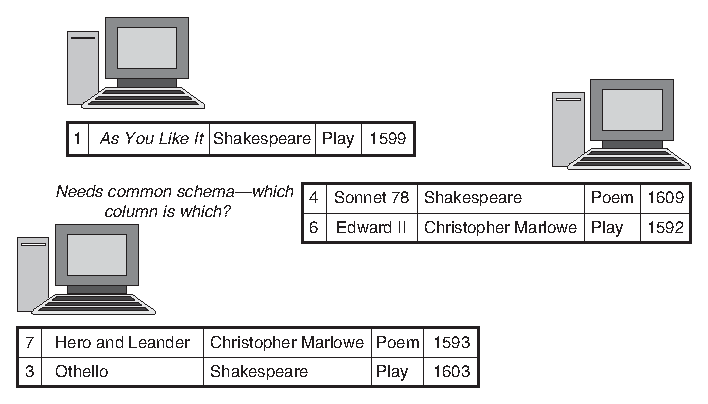
\includegraphics[width=5.0in]{media/ch3/f03-01-9780123859655.eps}
    \caption{Distributing data across the Web, row by row.}
    \label{fig:ch3.1}
\end{figure}



\begin{figure}
    \centering
    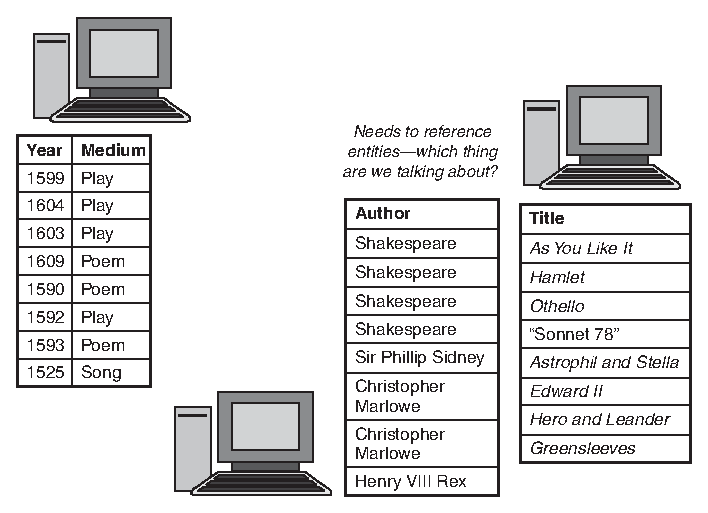
\includegraphics[width=5.0in]{media/ch3/f03-02-9780123859655.eps}
    \caption{Distributing data across the Web, column by column.}
    \label{fig:ch3.2}
\end{figure}



\begin{figure}
    \centering
    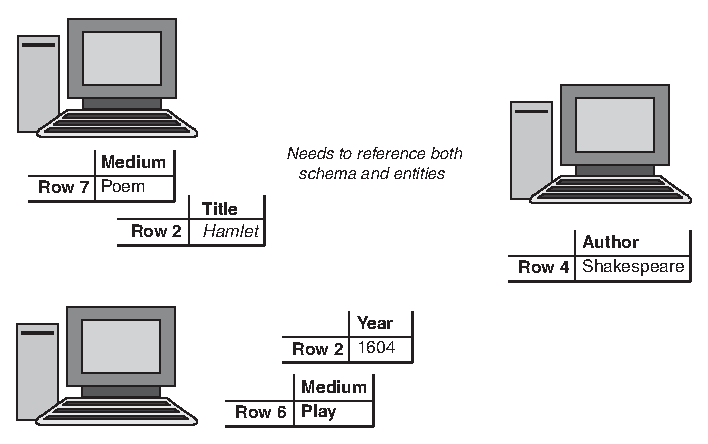
\includegraphics[width=5.0in]{media/ch3/f03-03-9780123859655.eps}
    \caption{Distributing data across the Web, cell by cell.}
    \label{fig:ch3.3}
\end{figure}



Figure~\ref{fig:ch3.2} shows another strategy, in which each server is responsible
for one or more complete columns from the original table. In this
example, one server is responsible for the publication dates and medium,
and another server is responsible for titles. This solution is flexible
in a different way from the solution of Figure~\ref{fig:ch3.1}. The solution in
Figure~\ref{fig:ch3.2} allows each machine to be responsible for one kind of
information. If we are not interested in the dates of publication, we
needn't consider information from that server. If we want to specify
something new about the entities (say, how many pages the manuscript
is), we can add a new server with that information without disrupting
the others.

This solution is similar to the solution in Figure~\ref{fig:ch3.1} in that it
requires some coordination between the servers. In this case, the
coordination has to do with the identities of the entities to be
described. How do I know that row 3 on one server refers to the same
entity as row 3 on another server? This solution requires a global
identifier for the entities being described.

The strategy outlined in Figure~\ref{fig:ch3.3} is a combination of the previous two
strategies, in which information is neither distributed row by row nor
column by column but instead is distributed cell by cell. Each machine
is responsible for some number of cells in the table. This system
combines the flexibility of both of the previous strategies. Two servers
can share the description of a single entity (in the figure, the year
and title of Hamlet are stored separately), and they can share the use
of a particular property (in Figure~\ref{fig:ch3.3}, the Medium of rows 6 and 7 are
represented on different servers).

This flexibility is required if we want our data distribution system to
really support the AAA slogan that ``Anyone can say Anything about Any topic.'' If we take the AAA
slogan seriously, any server needs to be able to make a statement about
any entity (as is the case in Figure~\ref{fig:ch3.2}), but also any server needs to
be able to specify any property of an entity (as is the case in Figure~\ref{fig:ch3.1}). The solution in Figure~\ref{fig:ch3.3} has both of these benefits.


\begin{table}[h]
\centering
\begin{tabular}{||l l l||} 
 \hline
Subject&Predicate&Object \\ [0.5ex] 
 \hline\hline
Row 7&Medium&Poem \\
Row 2&Title&Hamlet \\
Row 2&Year&1604\\
Row 4&Author&Shakespeare\\
Row 6&Medium&Play\\

\hline
\end{tabular}
\caption{Sample triples}
\label{tab:ch3.2}
\end{table}





But this solution also combines the costs of the other two strategies.
Not only do we now need a global reference for the column headings, but
we also need a global reference for the rows. In fact, each cell has to
be represented with three values: a global reference for the row, a
global reference for the column, and the value in the cell itself. This
third strategy is the strategy taken by RDF. We will see how RDF
resolves the issue of global reference later in this chapter, but for
now, we will focus on how a table cell is represented and managed in
RDF.

Since a cell is represented with three values, the basic building block
for RDF is called the \emph{triple}. The identifier for the row is called the
\emph{subject} of the triple (following the notion from elementary grammar,
since the subject is the thing that a statement is about). The
identifier for the column is called the \emph{predicate} of the triple (since
columns specify properties of the entities in the rows). The value in
the cell is called the \emph{object} of the triple. Table~\ref{tab:ch3.2} shows the triples
in Figure~\ref{fig:ch3.3} as subject, predicate, and object.

Triples become more interesting when more than one triple refers to the
same entity, such as in Table~\ref{tab:ch3.3}. When more than one triple refers to
the same thing, sometimes it is convenient to view the triples as a
directed graph in which each triple is an edge from its subject to its
object, with the predicate as the label on the edge, as shown in Figure~\ref{fig:ch3.4}. The graph 
visualization in Figure~\ref{fig:ch3.4} expresses the same
information presented in Table~\ref{tab:ch3.3}, but everything we know about
Shakespeare (either as subject or object) is displayed at a single node.

\begin{table}[h]
\centering
\begin{tabular}{||l l l||} 
 \hline
 Subject&Predicate&Object \\ [0.5ex] 
 \hline\hline
Shakespeare&wrote&King Lear \\
Shakespeare&wrote&Macbeth \\
Anne Hathaway&married&Shakespeare \\
Shakespeare&livedIn&Stratford \\
Stratford&isIn&England\\
Macbeth&setIn&Scotland\\
England&partOf&UK \\
Scotland&partOf&UK \\
\hline
\end{tabular}
\caption{Sample triples}
\label{tab:ch3.3}
\end{table}




\begin{figure}
    \centering
    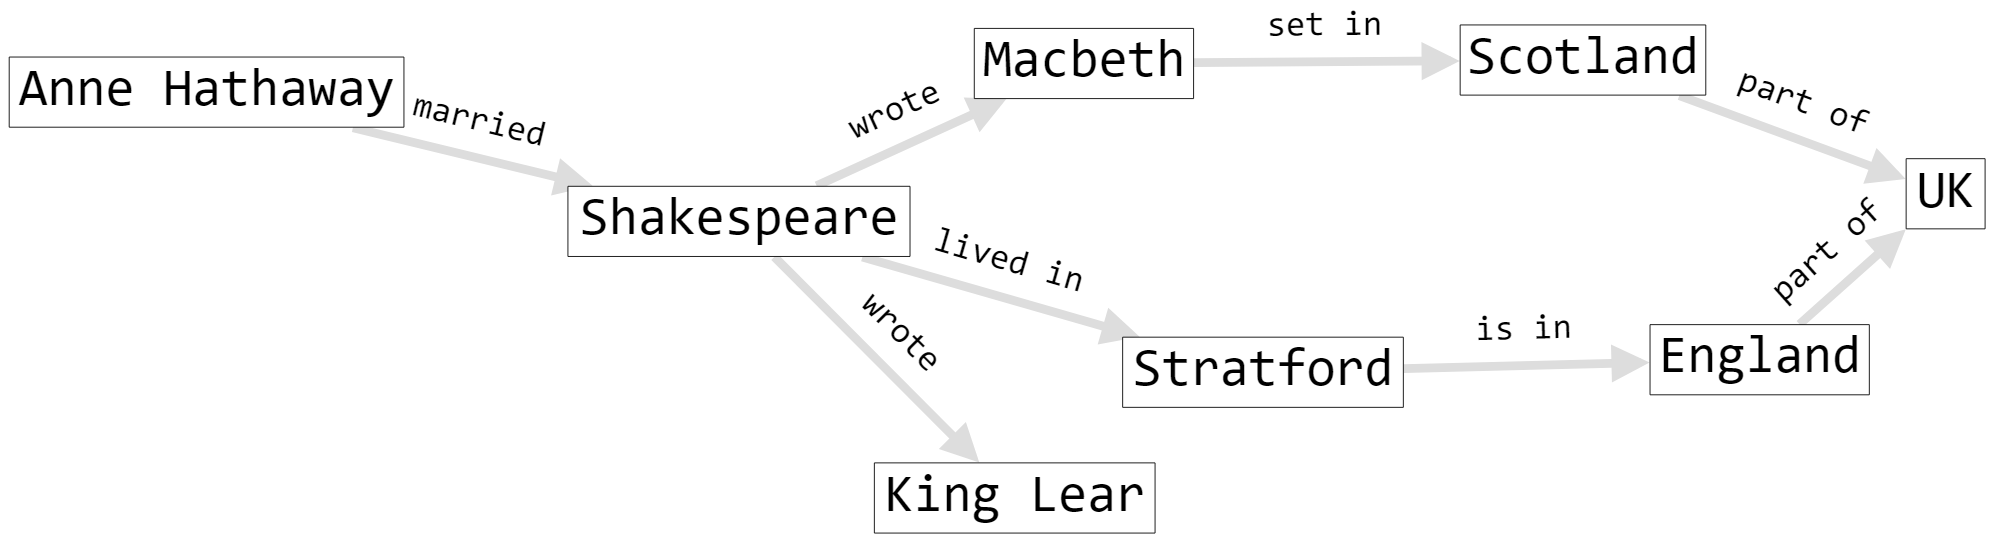
\includegraphics[width=5.0in]{SWWOv3/media/ch3/figure3-4.png}
    \caption{Graph display of triples from Table \ref{tab:ch3.3}. Eight triples appear as eight labeled edges.}
    \label{fig:ch3.4}
\end{figure}


\section{Merging Data from Multiple Sources}

We started off describing RDF as a way to distribute data over several
sources. But when we want to use that data, we will need to merge those
sources back together again. One value of the triples representation is
the ease with which this kind of merger can be accomplished. Since
information is represented simply as triples, merged information from
two graphs is as simple as forming the graph of all of the triples from
each individual graph, taken together. Let's see how this is
accomplished in RDF.

Suppose that we had another source of information that was relevant to
our example from Table~\ref{tab:ch3.3}---that is, a list of plays that Shakespeare wrote or a list of parts
of the United Kingdom. These would be represented as triples as in
Tables~\ref{tab:ch3.4} and \ref{tab:ch3.5}. Each of these can also be shown as a graph, just as
in the original table, as shown in Figure~\ref{fig:ch3.5}.

What happens when we merge together the information from these three
sources? We simply get the graph of all the triples that show up in
Figures \ref{fig:ch3.4} and \ref{fig:ch3.5}. Merging graphs like those in 
Figures \ref{fig:ch3.4} and \ref{fig:ch3.5} to
create a combined graph like the one shown in Figure~\ref{fig:ch3.6} is a
straightforward process---but only when it is known which nodes in each
of the source graphs match.

\begin{table}[h]
\centering
\begin{tabular}{||l l l||} 
 \hline
 Subject&Predicate&Object \\ [0.5ex] 
 \hline\hline
Scotland&part Of&The UK \\
England&part Of&The UK \\
Wales&part Of&The UK\\
Northern Ireland&part Of&The UK \\
Channel Islands&part Of&The UK\\
Isle of Man&part Of&The UK\\
\hline
\end{tabular}
\caption{Triples about the Parts of the United Kingdom}
\label{tab:ch3.5}
\end{table}

\begin{table}[h]
\centering
\begin{tabular}{||l l l||} 
 \hline
 Subject&Predicate&Object \\ [0.5ex] 
 \hline\hline
Shakespeare&wrote&As You Like It\\
Shakespeare&wrote&Henry V\\
Shakespeare&wrote&Love's Labour's Lost \\
Shakespeare&wrote&Measure for Measure \\
Shakespeare&wrote&Twelfth Night \\
Shakespeare&wrote&The Winter's Tale \\
Shakespeare&wrote&Hamlet\\
Shakespeare&wrote&Othello\\
\hline
\end{tabular}
\caption{Triples about Shakespeare's Plays}
\label{tab:ch3.4}
\end{table}


\begin{figure}
    \centering
    (a)
    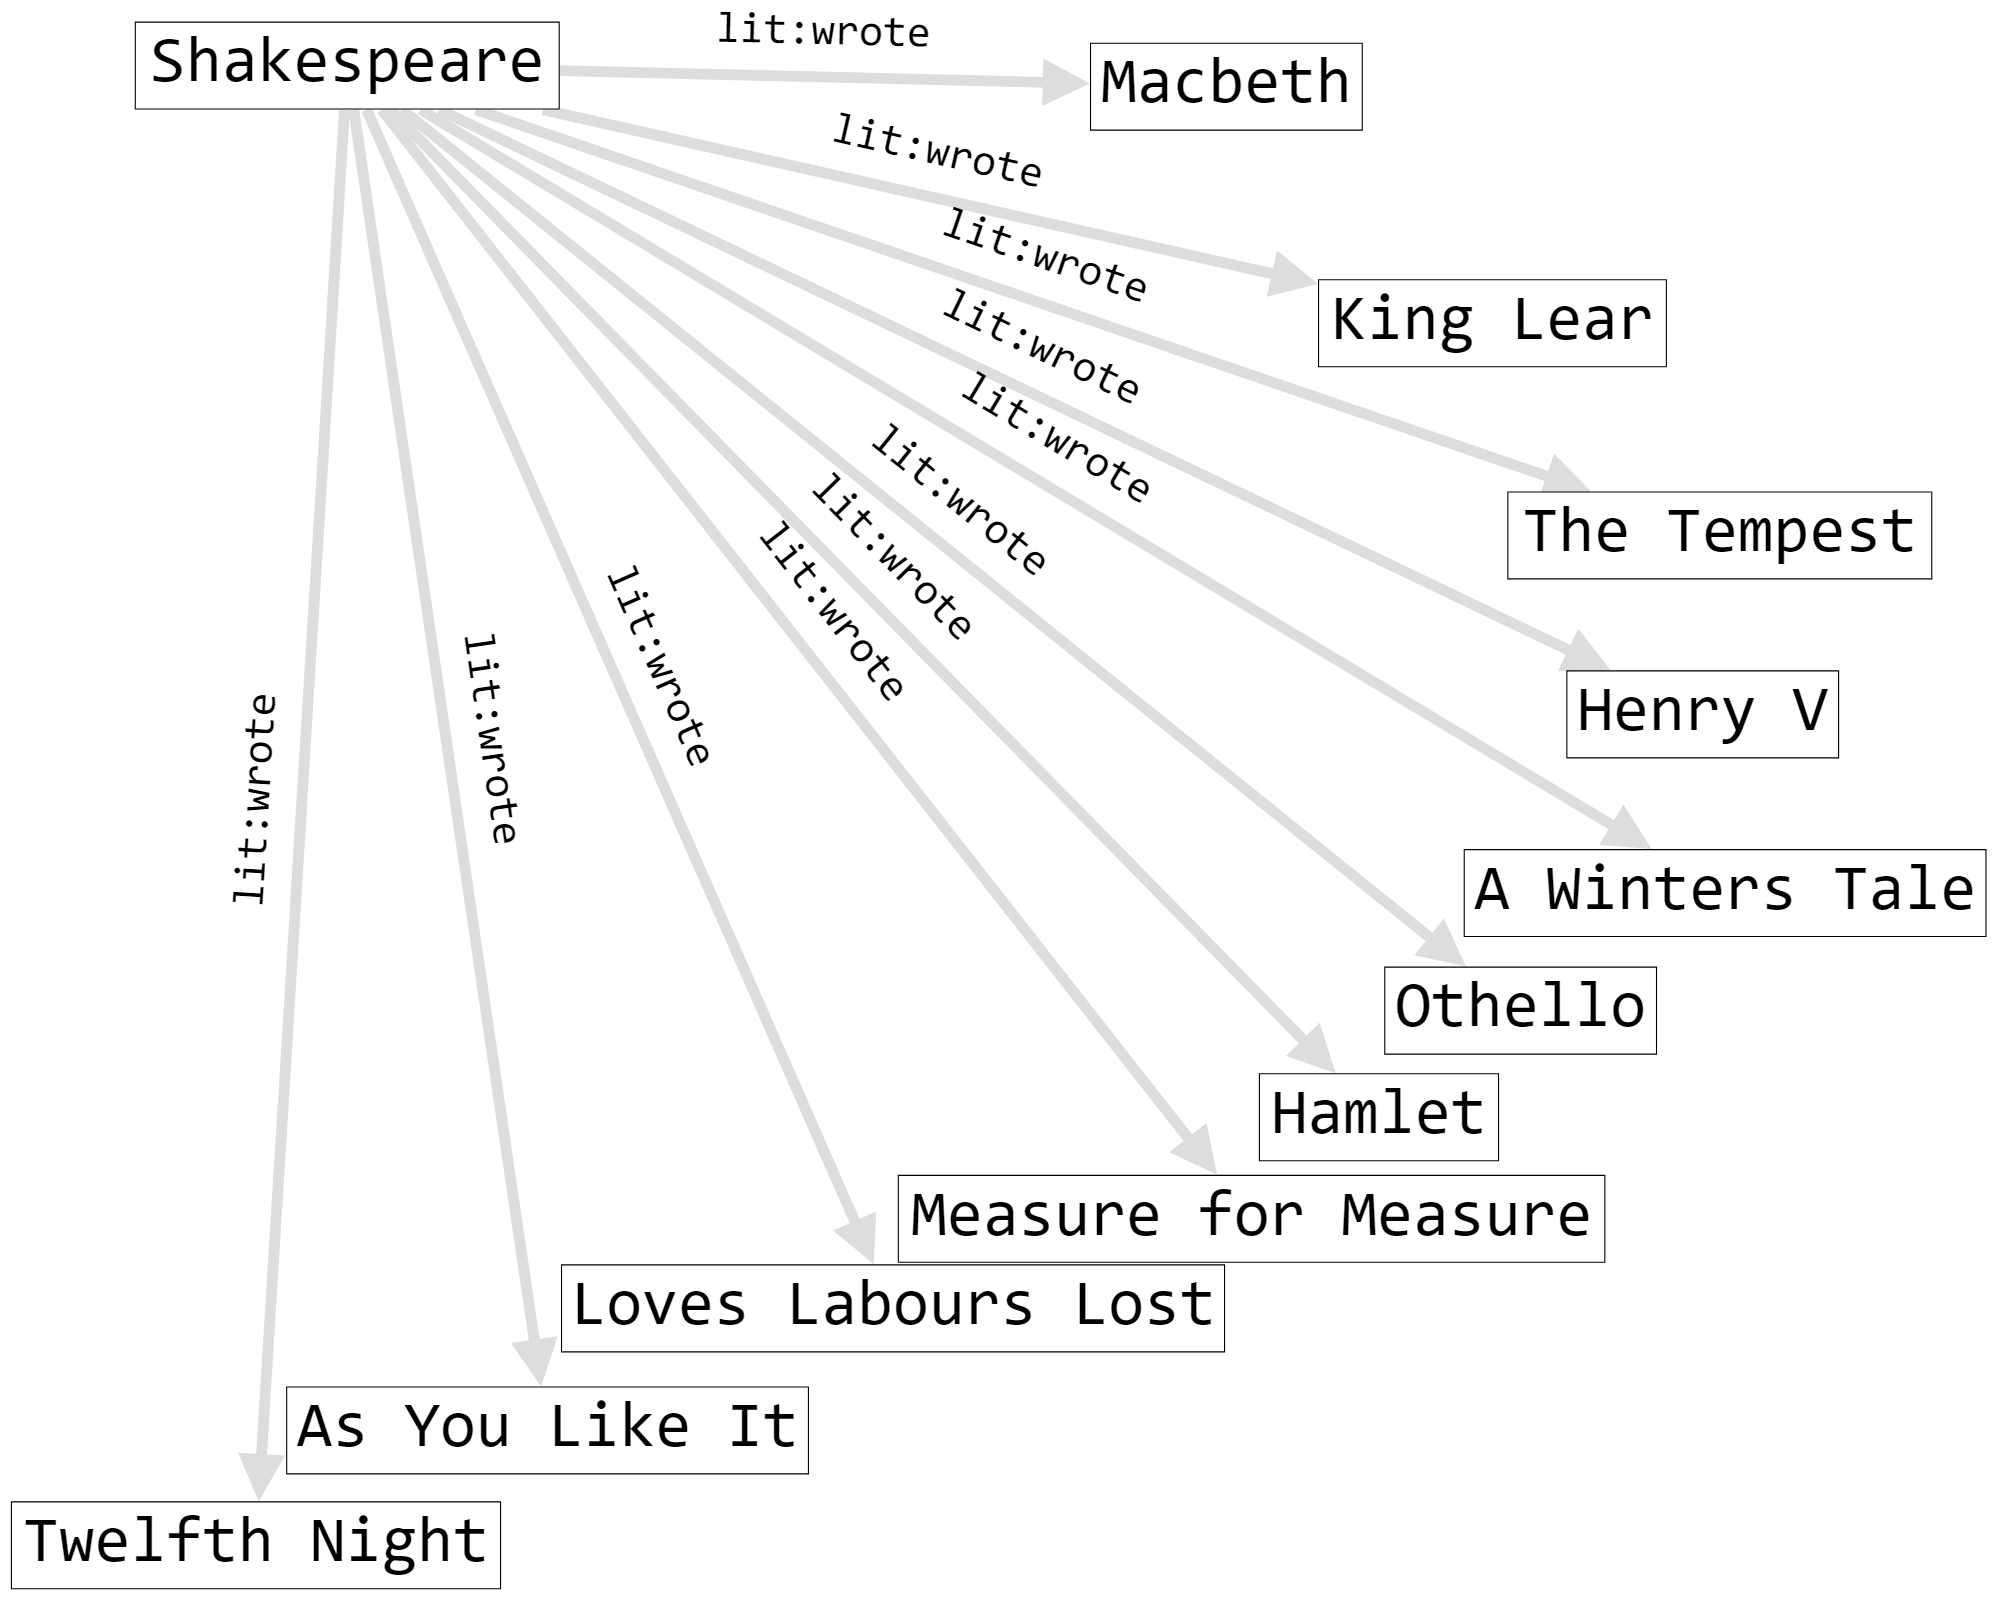
\includegraphics[width=5.0in]{SWWOv3/media/ch3/figure3-5a.png}
    (b)
    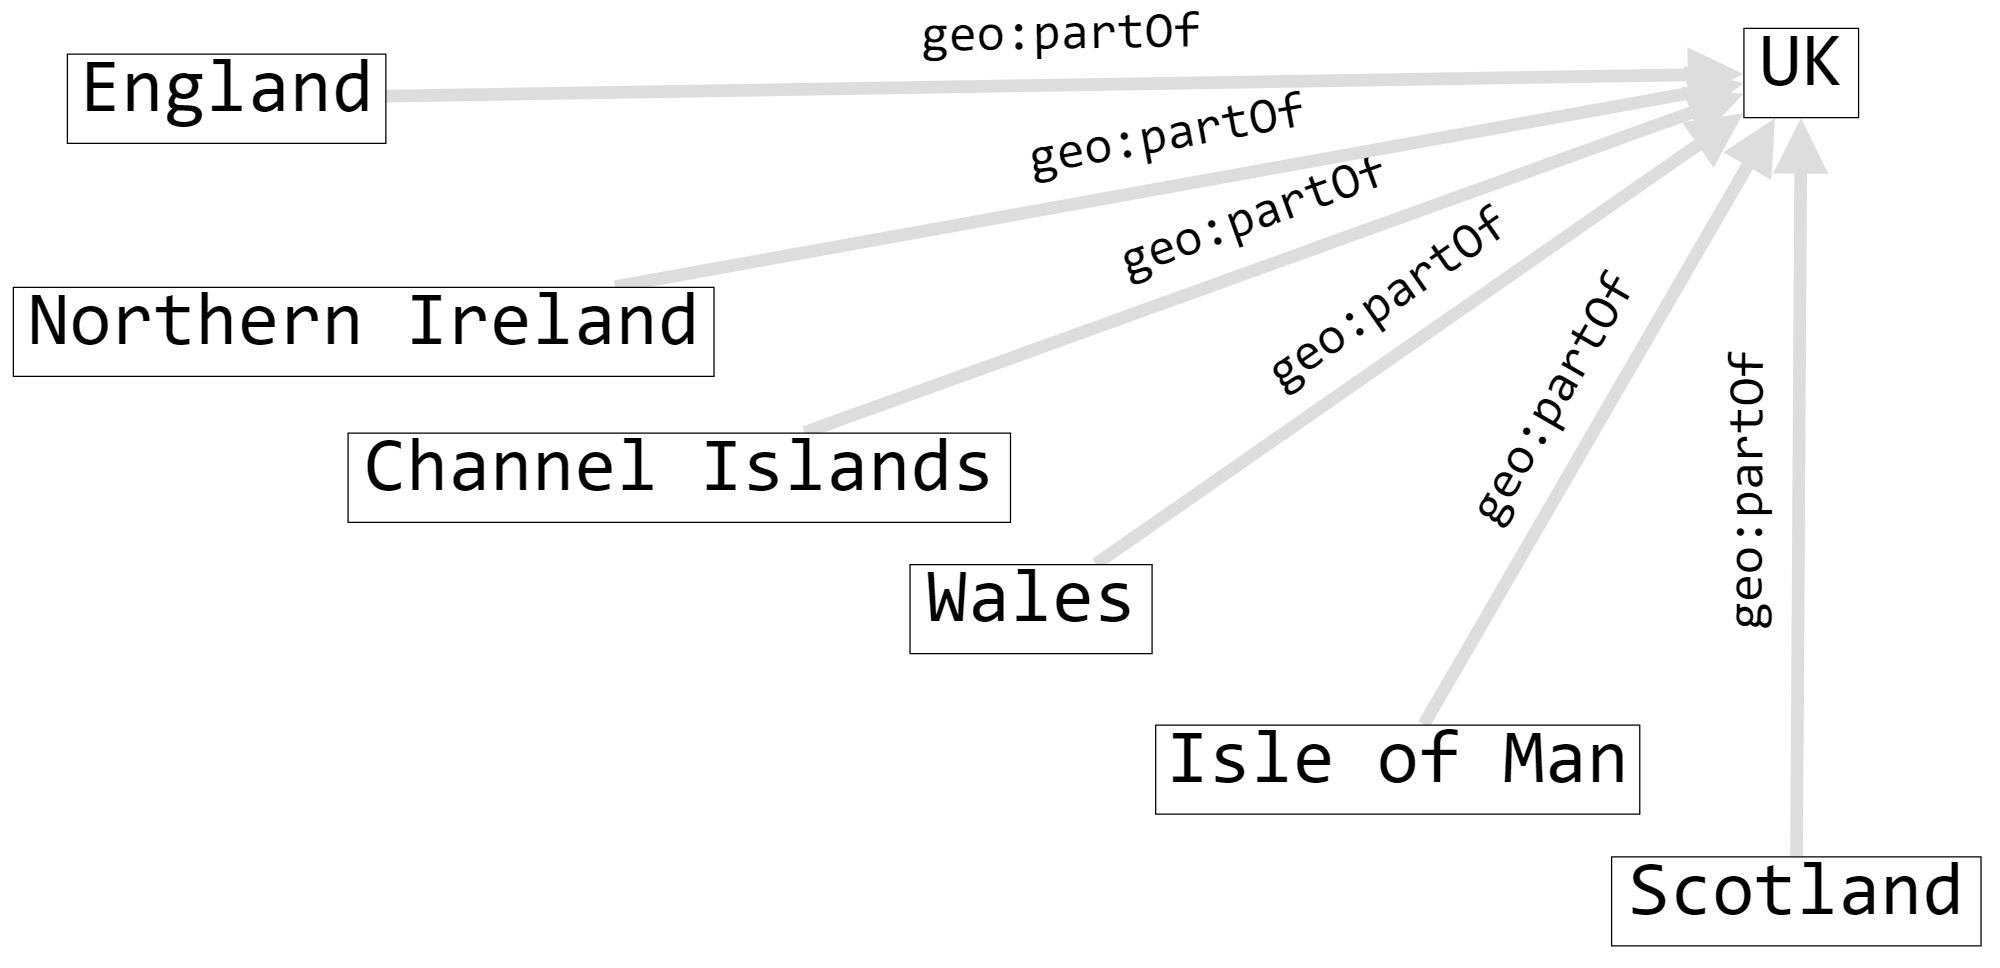
\includegraphics[width=5.0in]{SWWOv3/media/ch3/figure3-5b.png}
    \caption{Graphic representation of triples describing (a) Shakespeare’s plays and (b) parts of the United Kingdom.}
    \label{fig:ch3.5}
\end{figure}


\begin{figure}
    \centering
    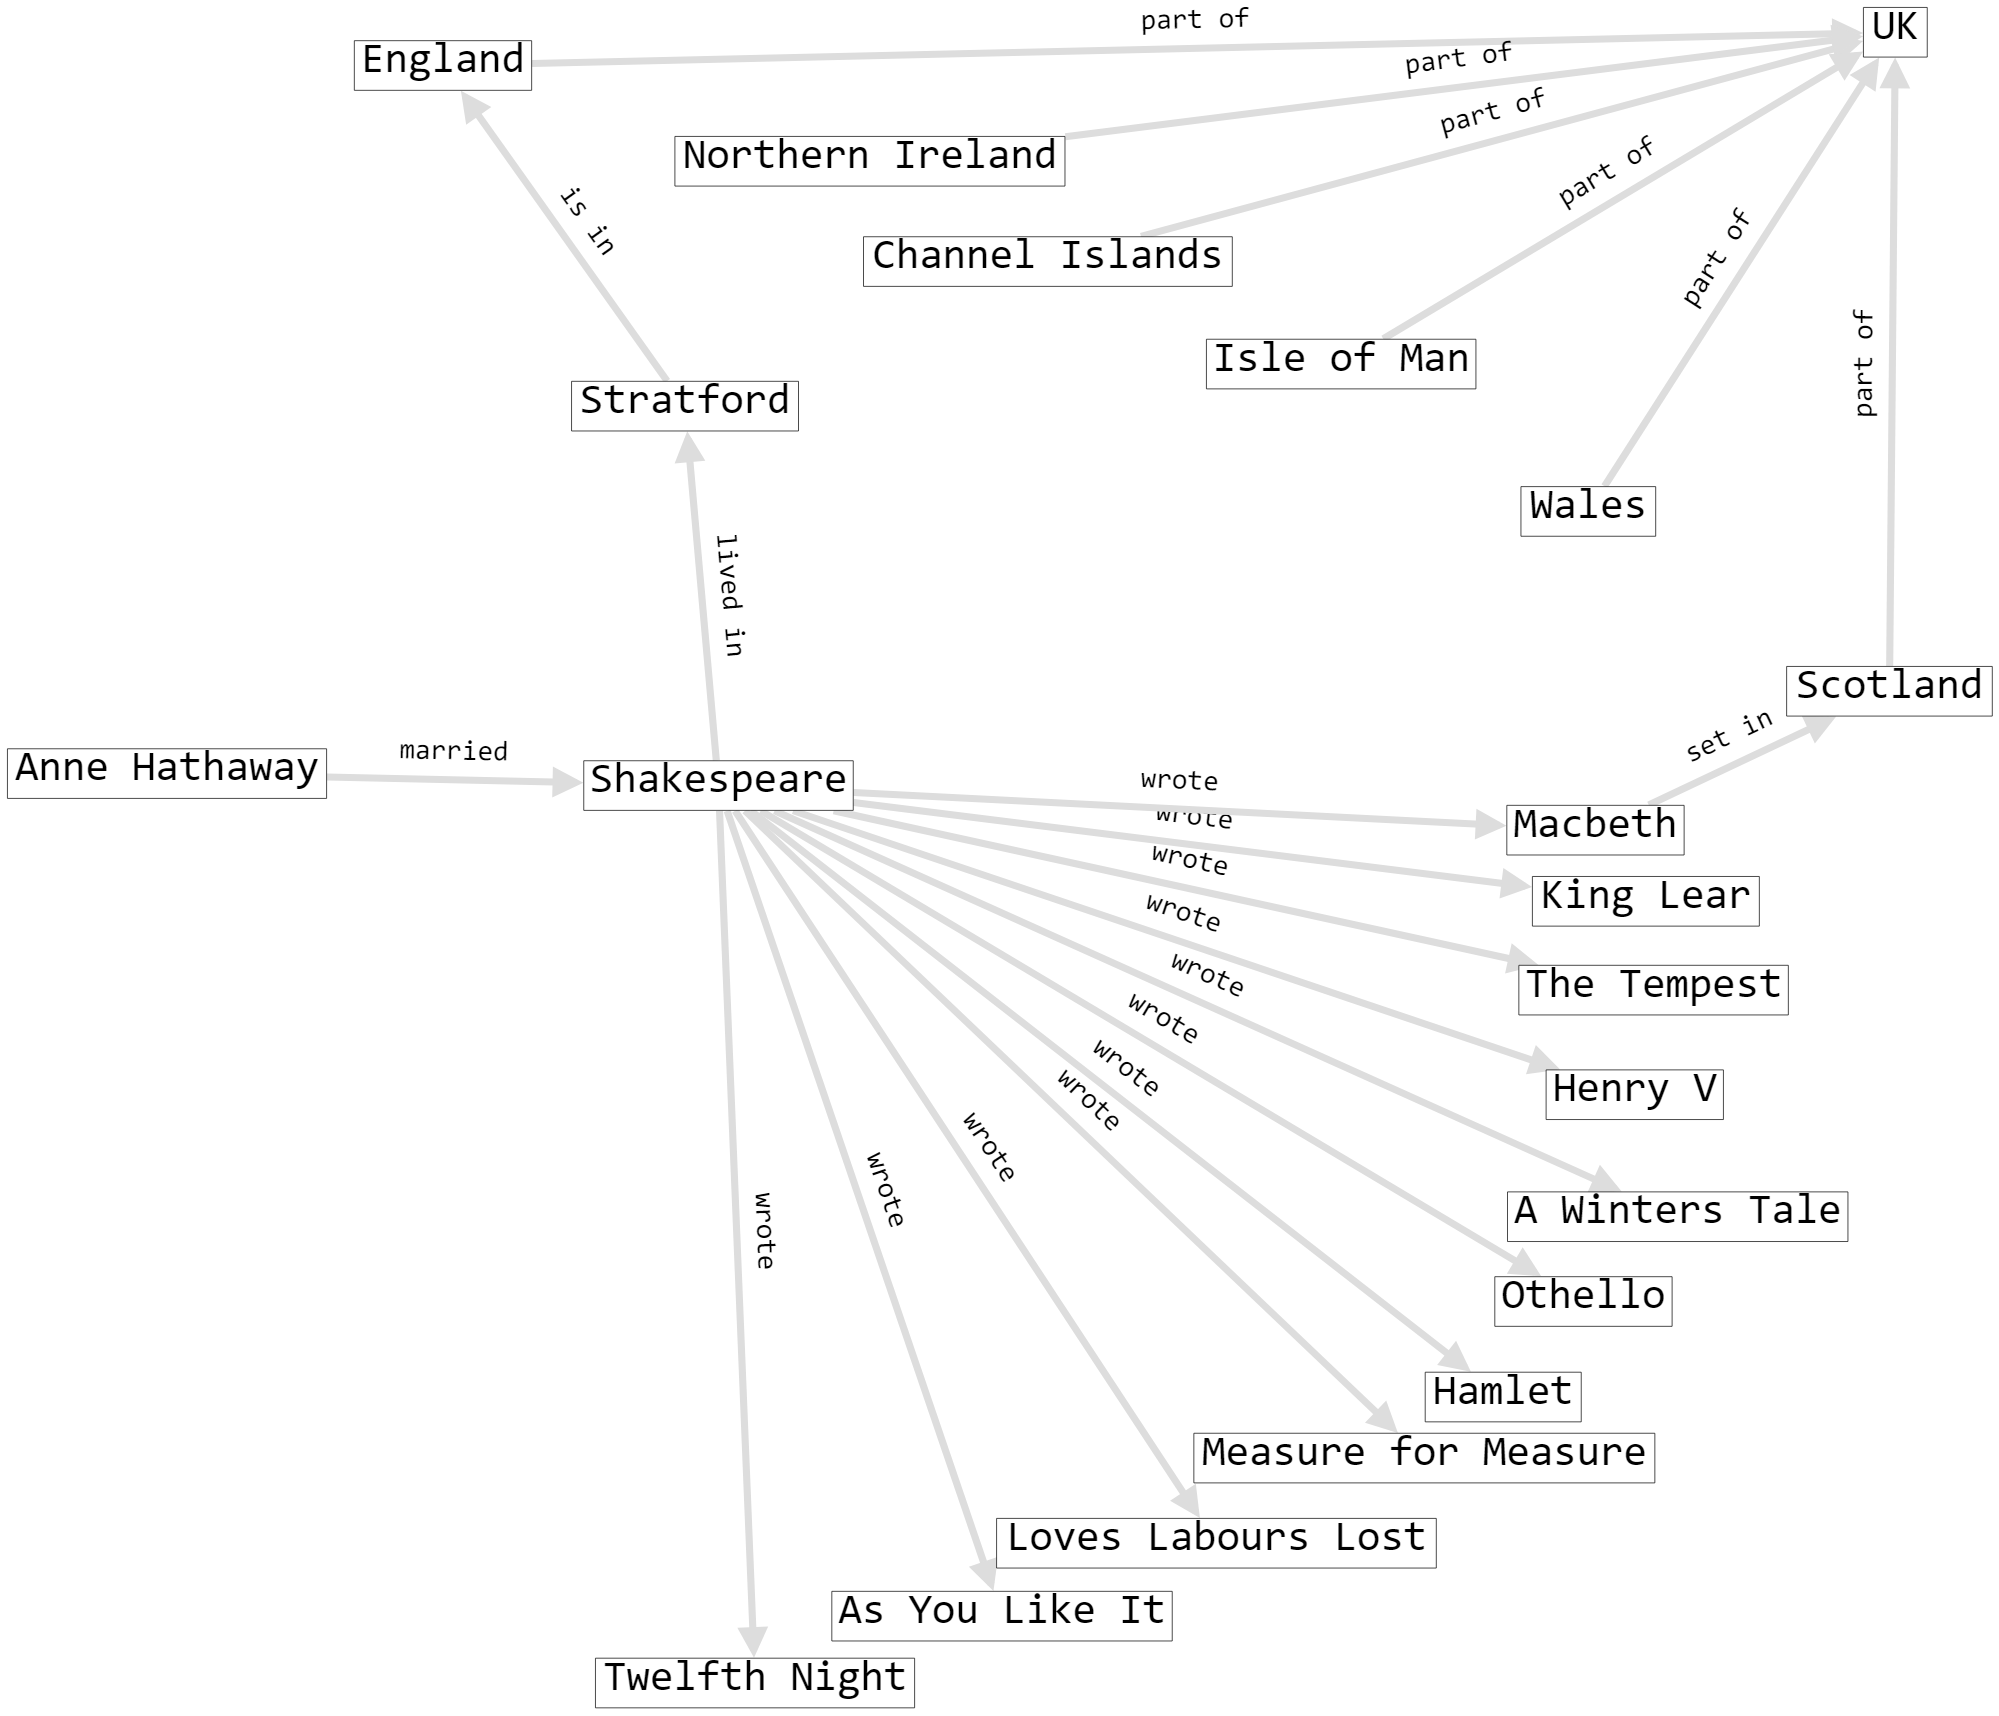
\includegraphics[width=5.0in]{SWWOv3/media/ch3/figure3-6.png}
    \caption{Combined graph of all triples about Shakespeare and the United Kingdom.}
    \label{fig:ch3.6}
\end{figure}



\section{Namespaces, Uris, and Identity}

The essence of the merge process comes down to answering the question ``When is
a node in one graph the same node as a node in another graph?'' In RDF,
this issue is resolved through the use of Uniform Resource Identifiers
(URIs).

In the figures so far, we have labeled the nodes and edges in the graphs
with simple names like \emph{Shakespeare} or \emph{Wales}. On the Semantic Web, this
is not sufficient information to determine whether two nodes are really
the same. Why not? Isn't there just one thing in the universe that
everyone agrees refers to as \emph{Shakespeare}? When referring to agreement on
the Web, never say, ``everyone.'' Somewhere, someone will refer not to
the historical Shakespeare but to the title character of the feature
film \emph{Shakespeare in Love}, which bears very little resemblance to
the historical figure. And ``Shakespeare'' is one of the more stable
concepts to appear on the Web; consider the range of referents for a
name like ``Washington'' or ``Bordeaux.'' To merge graphs in a Semantic
Web setting, we have to be more specific: In what sense do we mean the
word \emph{Shakespeare}?

RDF borrows its solution to this problem from foundational Web
technology --- in particular, the \emph{URI}. The basic syntax and format of a URI are
familiar even to casual users of the Web today because of the special,
but typical, case of the URL --- for example,
\texttt{http://www.workingontologist.org/Examples/Chapter3/Shakespeare\#Shakespeare}. 
But the significance of the URI as a
global identifier for a Web resource is often not appreciated. A URI
provides a global identification for a resource that is common across
the Web. This is not a stipulation that is particular to the Semantic
Web but to the Web in general; global naming leads to global network
effects. Of course, in the jungle that is the web, we can't expect that
every data source that refers to Shakespeare will use the same URI.  In
Chapter~\ref{ch5} we will explore when and why we might use different URIs for
the same individual, and what capabilities the Semantic Web provides to
manage them.

URIs and URLs look exactly the same, and, in fact, a URL is just a
special case of the URI. Why does the Web have both of these ideas?
Simplifying somewhat, the URI is an identifier with global (i.e.,
``World Wide'' in the ``World Wide Web'' sense) scope. Any two Web
applications in the world can refer to the same thing by referencing the
same URI. But the syntax of the URI makes it possible to ``dereference''
it---that is, to use all the information in the URI (which specifies
things like server name, protocol, port number, file name, etc.) to
locate a file (or a location in a file) on the Web \footnote{We are primarily discussing files here, but a URI can refer to other
resources. The Wikipedia article on URIs includes more than 50 different
resource types that can be referenced by URIs---see
\url{http://en.wikipedia.org/wiki/URI_} scheme.}. This
dereferencing succeeds if all these parts work; the protocol locates the
specified server running on the specified port and so on. When this is
the case, we can say that the URI is not just a URI, but an effective
HTTP URI. From the point of view of modeling, the distinction is not
important. But from the point of view of having a model on the Semantic
Web, the fact that a URI can potentially be dereferenced allows the
models to participate in a global Web infrastructure as we will see in
chapter~\ref{ch5}

The URI can be generalized further as an Internationalized Resource Identifier, 
or IRI.  The IRI is a generalization of the URI that uses all the character representations
for languages on the web, so an IRI can include characters with accents or indeed chacters from 
any language that has a standard web encoding. 

RDF applies the notion of the URI to resolve the identity problem in
graph merging. The application is quite simple: A node from one graph is
merged with a node from another graph exactly if they have the same
URI. On the one hand, this may seem disingenuous, ``solving'' the
problem of node identity by relying on another standard to solve it. On
the other hand, since issues of identity appear in the Web in general
and not just in the Semantic Web, it would be foolish not to use the
same strategy to resolve the issue in both cases.

\subsection{Expressing URIs in print}

URIs work very well for expressing identity on the World Wide Web, but
they are typically a bit of a pain to write out in detail when
expressing models, especially in print. So for the examples in this
book, we use a simplified version of a URI abbreviation scheme called
\emph{CURIEs} (standing for \emph{Compact URI}). In its simplest form, a
URI expressed as a CURIE has two parts: a namespace and an identifier,
written with a colon between. So the CURIE representation for the
identifier \emph{England} in the namespace \emph{geo} is simply \texttt{geo:England}.
The RDF standard syntaxes include elaborate rules that allow programmers
to map namespaces to other URI representations (such as the familiar
\emph{http://} notation). For the examples in this book, we will use the
simple CURIE form for all URIs. It is important, however, to note that
CURIEs are \emph{not} global identifiers on the Web; only fully
qualified URIs (e.g.
\emph{http://www.WorkingOntologist.org/Examples/Chapter3/Shakespeare\#Shakespeare})
are global Web names. Thus, any representation of a CURIE must, in
principle, be accompanied by a declaration of the namespace
correspondence.

It is customary on the Web in general
to insist that URIs contain no embedded spaces. For example, an
identifier ``part of'' is typically not used in the web. Instead, we
follow the InterCap convention (sometimes called CamelCase), whereby
names that are made up of multiple words are transformed into
identifiers without spaces by capitalizing each word. Thus, ``part of''
becomes partOf, ``Great Britain'' becomes GreatBritain, ``Measure for
Measure'' becomes MeasureForMeasure, and so on.

There is no limitation on the use of multiple namespaces in a single
source of data, or even in
a single triple. Selection of namespaces is entirely unrestricted as far
as the data model and standards are concerned. It is common practice,
however, to refer to related identifiers in a single namespace. For
instance, all of the literary or geographical information from Table~\ref{tab:ch3.4}
or Table~\ref{tab:ch3.5} would be placed into one namespace per table, with a
suggestive name---say, \emph{lit} or \emph{geo}---respectively. Strictly
speaking, these names correspond to fully qualified URIs---for example,
\emph{lit} stands for \emph{http://www.WorkingOntologist.com/Examples/Chapter3/Shakespeare\#}, and
\emph{geo} stands for \emph{http://www.WorkingOntologist.com/Examples/Chapter3/geography\#}.


For the purposes of explaining modeling on the Semantic Web, the
detailed URIs behind the CURIEs are not important, so for the most part,
we will omit these bindings from now on. In many examples, we will take
this notion of abbreviation one step further; in the cases when we use a
single namespace throughout one example, we will assume there is a
default namespace declaration that allows us to refer to URIs simply
with a symbolic name preceded by a colon (:), such as :Shakespeare,
:JamesDean, :Researcher.

\begin{table}[h]
\centering
\begin{tabular}{||l l l ||} 
 \hline
 Subject&Predicate&Object \\ [0.5ex] 
 \hline\hline
lit:Shakespeare&lit:wrote&lit:AsYouLikeIt\\
lit:Shakespeare&lit:wrote&lit:HenryV\\
lit:Shakespeare&lit:wrote&lit:LovesLaboursLost\\
lit:Shakespeare&lit:wrote&lit:MeasureForMeasure\\
lit:Shakespeare&lit:wrote&lit:TwelfthNight\\
lit:Shakespeare&lit:wrote&lit:WintersTale\\
lit:Shakespeare&lit:wrote&lit:Hamlet\\
lit:Shakespeare&lit:wrote&lit:Othello\\
\hline
\end{tabular}
\caption{Plays of Shakespeare with CURIEs}
\label{tab:ch3.6}
\end{table}



\begin{table}[h]
\centering
\begin{tabular}{||l l l ||} 
 \hline
 Subject&Predicate&Object \\ [0.5ex] 
 \hline\hline
geo:Scotland&geo:partOf&geo:UK \\
geo:England&geo:partOf&geo:UK \\
geo:Wales&geo:partOf&geo:UK \\
geo:NorthernIreland&geo:partOf&geo:UK \\
geo:ChannelIslands&geo:partOf&geo:UK \\
geo:IsleOfMan&geo:partOf&geo:UK \\
\hline
\end{tabular}
\caption{Geographical names with CURIEs}
\label{tab:ch3.7}
\end{table}

Using CURIEs, our triple sets now look as shown in Tables~\ref{tab:ch3.6} and \ref{tab:ch3.7}.
Compare Table~\ref{tab:ch3.6} with Table~\ref{tab:ch3.4}, and compare Table~\ref{tab:ch3.7} with Table~\ref{tab:ch3.5}.
But it isn't always that simple; some triples will have to use
identifiers with different namespaces, as in the example in Table~\ref{tab:ch3.8},
which was taken from Table~\ref{tab:ch3.3}.

In Table~\ref{tab:ch3.8}, we introduced a new namespace, \emph{bio:}, without
specifying the actual URI to which it corresponds. For this model to
participate on the Web, this information must be filled in. But from the
point of view of modeling, this detail is unimportant. For the rest of
this book, we will assume that the prefixes of all CURIEs are defined,
even if that definition has not been specified explicitly in print.

\subsection{Standard namespaces}

Using the URI as a standard for global identifiers allows for a
worldwide reference for any symbol. This means that we can tell when any
two people anywhere in the world are referring to the same thing.

This property of the URI provides a simple way for a standard
organization (like the W3C) to specify the meaning of certain terms in
the standard. As we will see in coming chapters, the W3C standards
provide definitions for terms such as type, subClassOf, Class,
inverseOf, and so forth. But these standards are intended to apply
globally across the Semantic Web, so the standards refer to these reserved words in the same way as they refer to any other
resource on the Semantic Web, as URIs.

\begin{table}[h]
\centering
\begin{tabular}{||l l l ||} 
 \hline
 Subject&Predicate&Object \\ [0.5ex] 
 \hline\hline
lit:Shakespeare&lit:wrote&lit:KingLear\\
lit:Shakespeare&lit:wrote&lit:MacBeth\\
bio:AnneHathaway&bio:married&lit:Shakespeare\\
bio:AnneHathaway&bio:livedWith&lit:Shakespeare\\
lit:Shakespeare&bio:livedIn&geo:Stratford\\
geo:Stratford&geo:isIn&geo:England\\
geo:England&geo:partOf&geo:UK\\
geo:Scotland&geo:partOf&geo:UK\\
\hline
\end{tabular}
\caption{Triples Referring to URIs with a Variety of Namespaces}
\label{tab:ch3.8}
\end{table}



The W3C has defined a number of standard namespaces for use with Web
technologies, including \emph{xsd:} for XML schema definition;
\emph{xmlns:} for XML namespaces; and so on. The Semantic Web is handled
in exactly the same way, with namespace definitions for the major layers
of the Semantic Web. Following standard practice with the W3C, we will
use CURIEs to refer to these terms, using the following definitions for
the standard namespaces.

\emph{rdf}: Indicates identifiers used in RDF. The set of identifiers defined
in the standard is quite small and is used to define types and
properties in RDF. The global URI for the rdf namespace is http://
\href{http://www.w3.org/1999/02/22-rdf-syntax-ns}{www.w3.org/1999/02/22-rdf-syntax-ns\#.}

\emph{rdfs}: Indicates identifiers used for the RDF Schema language, RDFS. The
scope and semantics of the symbols in this namespace are the topics of
future chapters. The global URI for the rdfs namespace is
\href{http://www.w3.org/2000/01/rdf-schema}{http://www.w3.org/2000/01/rdf-schema\#.}

\emph{skos}: Indicates identifiers used for the Simple Knowledge Organization System (SKOS), a schema for
distributed management of vocabularies on the web.  
Chapter~\ref{ch11} provides a detailed discussion on SKOS and it's use.   The global URI  for SKOS  is
\texttt{http://www.w3.org/2004/02/skos/core}


\emph{owl}: Indicates identifiers used for the Web Ontology Language, OWL. The
scope and semantics of the symbols in this namespace are the topics of
future chapters. The global URI for the owl namespace is
\href{http://www.w3.org/2002/07/owl}{http://www.w3.org/2002/07/owl\#.}

These URIs provide a good example of the interaction between a URI and a
URL. For modeling purposes, any URI in one of these namespaces (e.g.,
\emph{http://www.w3.org/2000/01/rdf-schema\#subClassOf}, or
\texttt{rdfs:subClassOf} for short) refers to a particular term that the W3C
makes some statements about in the RDFS standard. But the term can also
be dereferenced---that is, if we look at the server
\texttt{www.w3.org}, there is a page at the location
\texttt{2000/01/rdf-schema} with an entry about \texttt{subClassOf}, giving supplemental
information about this resource. From the point of view of modeling, it
is not necessary that it be possible to dereference this URI, but from
the point of view of Web integration, it is critical that it is. The
underlying standards and principles to weave such a Web of linked data
will be detailed in chapter~\ref{ch5}.
% Check this once you read ch 5

\section{Identifiers in the RDF Namespace}

The RDF data model specifies the notion of triples and the idea of
merging sets of triples as just shown. With the introduction of
namespaces, RDF uses the infrastructure of the Web to represent
agreements on how to refer to a particular entity. The RDF standard itself takes
advantage of the namespace infrastructure to define a small number of
standard identifiers in a namespace defined in the standard, a namespace
called rdf.


\begin{table}[h]
\centering
\begin{tabular}{||l l l ||} 
 \hline
 Subject&Predicate&Object \\ [0.5ex] 
 \hline\hline
lit:Shakespeare&rdf:type&lit:Playwright \\
lit:Ibsen&rdf:type&lit:Playwright \\
lit:Simon&rdf:type&lit:Playwright \\
lit:Miller&rdf:type&lit:Playwright \\
lit:Marlowe&rdf:type&lit:Playwright \\
lit:Wilder&rdf:type&lit:Playwright \\
\hline
\end{tabular}
\caption{Using rdf:type to Describe Playwrights}
\label{tab:ch3.9}
\end{table}


\begin{table}[h]
\centering
\begin{tabular}{||l l l ||} 
 \hline
 Subject&Predicate&Object \\ [0.5ex] 
 \hline\hline
lit:Playwright&rdf:type&bus:Profession \\
bus:Profession&rdf:type&hr:Compensation \\
\hline
\end{tabular}
\caption{Defining Types of Names}
\label{tab:ch3.10}
\end{table}



\texttt{rdf:type} is a property that provides an elementary typing system in RDF.
For example, we can express the relationship between several playwrights
using type information, as shown in Table~\ref{tab:ch3.9}. The subject of \texttt{rdf:type}
in these triples can be any identifier, and the object is understood to
be a type. There is no restriction on the usage of \texttt{rdf:type}
with types;
types can have types ad infinitum, as shown in Table~\ref{tab:ch3.10}.

When we read a triple out loud (or just to ourselves), it is
understandably tempting to read it (in English, anyway) in
subject/predicate/object order so that the first triple in Table~\ref{tab:ch3.9}
would read, ``Shakespeare type Playwright.'' Unfortunately, this is
pretty fractured syntax no matter how you inflect it. It would be better
to have something like ``Shakespeare has type Playwright'' or maybe
``The type of Shakespeare is Playwright.''

This issue really has to do with the choice of name for the \texttt{rdf:type}
resource; if it had been called rdf:isInstanceOf instead, it would have
been much easier to read out loud in English. But since we never have
control over how other entities (in this case, the W3C) chose their
names, we don't have the luxury of changing these names. When we read
out loud, we just have to take some liberties in adding in connecting
words. So this triple can be pronounced, ``Shakespeare {[}has{]} type
Playwright,'' adding in the ``has'' (or sometimes, the word ``is'' works
better) to make the sentence into somewhat correct English. Later in
this chapter, we'll see the \emph{Turtle} syntax for writing RDF, in which a
shortcut has been introduced for this particular case: the keyword ``a''
can be used instead of rdf:type which makes the reading ever easier
``Shakespeare {[}is{]} a Playwright''.

\texttt{rdf:Property} is an identifier that is used as a type in RDF to indicate
when another identifier is to be used as a predicate rather than as a
subject or an object. We can declare all the identifiers we have used as
predicates so far in this chapter as shown in Table~\ref{tab:ch3.11}.

\begin{table}[h]
\centering
\begin{tabular}{||l l l ||} 
 \hline
 Subject&Predicate&Object \\ [0.5ex] 
 \hline\hline
lit:wrote&rdf:type&rdf:Property\\
geo:partOf&rdf:type&rdf:Property\\
bio:married&rdf:type&rdf:Property\\
bio:livedIn&rdf:type&rdf:Property\\
bio:livedWith&rdf:type&rdf:Property\\
geo:isIn&rdf:type&rdf:Property\\
\hline
\end{tabular}
\caption{rdf:Property Assertions for Tables 3.5 to 3.8}
\label{tab:ch3.11}
\end{table}

\section{CHALLENGES: RDF and Tabular Data}

We began this chapter by motivating RDF as a way to distribute data over
the Web---in particular, tabular data. Now that we have all of the
detailed mechanisms of RDF (including namespaces and triples) in place,
we can revisit tabular data and show how to represent it consistently in
RDF.

\begin{challenge}
\label{chal:1}

Given a table from a relational database, describing products,
suppliers, and stocking information about the products (see Table~\ref{tab:ch3.12}),
produce an RDF graph that reflects its contents in such a
way that the information intent is preserved but the data are now
amenable for RDF operations like merging and RDF query.

\solution

Each row in the table describes a single entity, all of the same type.
That type is given by the name of the table itself, Product. We know
certain information about each of these items, based on the columns in
the table itself, such as the model number, the division, and so on. We
want to represent these data in RDF.

Since each row represents a distinct entity, each row will have a
distinct URI. Fortunately, the need for unique identifiers is just as present in the database as it is in the
Semantic Web, so there is a (locally) unique identifier
available---namely, the primary table key, in this case the column
called ID. For the Semantic Web, we need a globally unique identifier.
The simplest way to form such an identifier is by having a single URI
for the database itself (perhaps even a URL if the database is on the
Web). Use that URI as the namespace for all the identifiers in the
database. We will discuss the minting of URIs more in details in chapter~\ref{ch5}. 
Since this is a database for a manufacturing company, let's call that
namespace mfg:.

\begin{table}[h]
\centering
\begin{tabular}{||l l l l l l l ||} 
 \hline
 ID&Machine Number&Division&ProductLine&Manufacture Location&SKU&Available \\ [0.5ex] 
 \hline\hline
1&ZX-3&Manufacturing support&Papermachine&Sacramento&FB3524&23\\
2&ZX-3P&Manufacturing support&Paper machine&Sacramento&KD5243&4\\
3&ZX-3S&Manufacturing support&Paper machine&Sacramento&IL4028&34\\
4&B-1430&Control Engineering&Feedback line&Elizabeth&KS4520&23\\
5&B-1430X&Control Engineering&Feedback line&Elizabeth&CL5934&14\\
6&B-1431&Control Engineering&Active sensor&Seoul&KK3945&0\\
7&DBB-12&Accessories&Monitor&Hong Kong&ND5520&100\\
8&SP-1234&Safety&Safety valve&Cleveland&HI4554&4\\
9&SPX-1234&Safety&Safety valve&Cleveland&OP5333&14\\
\hline
\end{tabular}
\caption{Sample Tabular Data for Triples}
\label{tab:ch3.12}
\end{table}



Then we can create an identifier for each line by concatenating the
table name ``Product'' with the unique key and expressing this
identifier in the \emph{mfg:} namespace, resulting in identifiers \texttt{mfg:Product1},
\texttt{mfg:Product2}, and so on.

Each row in the table says several things about that item---namely, its
model number, its division, and so on. To represent this in RDF, each of these will be a property that will
describe the Products. But just as is the case for the unique
identifiers for the rows, we need to have global unique identifiers for
these properties. We can use the same namespace as we did for the
individuals, but since two tables could have the same column name (but
they aren't the same properties!), we need to combine the table name and
the column name. This results in properties like \texttt{mfg:Product\_ModelNo},
\texttt{mfg:Product\_Division}, and so on.

With these conventions in place, we can now express all the information
in the table as triples. There will be one triple per cell in the
table---that is, for n rows and c columns, there will be n x c triples.
The data shown in Table~\ref{tab:ch3.12} have 7 columns and 9 rows, so there are 63
triples, as shown in Table~\ref{tab:ch3.13}.

The triples in the table are a bit different from the triples we have
seen so far. Although the subject and  
predicate of these triples are RDF resources (complete with CURIE
namespaces!), the objects are not resources but literal data---that is,
strings, integers, and so forth. This should come as no surprise, since,
after all, RDF is a data representation system. RDF borrows from XML all
the literal data types as possible values for the object of a triple; in
this case, the types of all data are strings or integers.

The usual interpretation of a table is that each row in the table
corresponds to one individual and that the type of these individuals
corresponds to the name of the table. In Table~\ref{tab:ch3.12}, each row
corresponds to a \texttt{Product}. We can represent this in RDF by adding one
triple per row that specifies the type of the individual described by
each row, as shown in Table~\ref{tab:ch3.14}.

The full complement of triples from the translation of the information
in Table~\ref{tab:ch3.12} is shown in Figure~\ref{fig:ch3.7}. The types (i.e., where the
predicate is \texttt{rdf:type}, and the object is the class \texttt{mfg:Product}) are
shown as links in the graph; triples in which the object is a literal
datum are shown (for sake of compactness in the figure) within a box
labeled by their common subject.

\begin{table}[h]
\centering
\begin{tabular}{||l l l ||} 
 \hline
 Subject&Predicate&Object \\ [0.5ex] 
 \hline\hline
mfg:Product1&mfg:Product\_ID&1 \\
mfg:Product1&mfg:Product\_ModelNo&ZX-3 \\
mfg:Product1&mfg:Product\_Division&Manufacturing support \\
mfg:Product1&mfg:Product\_Product\_Line&Paper machine \\
mfg:Product1&mfg:Product\_Manufacture\_Location&Sacramento \\
mfg:Product1&mfg:Product\_SKU&FB3524 \\
mfg:Product1&mfg:Product\_Available&23 \\
mfg:Product2&mfg:Product\_ID&2\\
mfg:Product2&mfg:Product\_ModelNo&ZX-3P\\
mfg:Product2&mfg:Product\_Division&Manufacturing support \\
mfg:Product2&mfg:Product\_Product\_Line&Paper machine \\
mfg:Product2&mfg:Product\_Manufacture\_Location&Sacramento\\
mfg:Product2&mfg:Product\_SKU&KD5243\\
mfg:Product2&mfg:Product\_Available&4\\
\hline
\end{tabular}
\caption{Triples Representing Some of the Data in Table \ref{tab:ch3.12}}
\label{tab:ch3.13}
\end{table}

\begin{table}[h]
\centering
\begin{tabular}{||l l l ||} 
 \hline
 Subject&Predicate&Object \\ [0.5ex] 
 \hline\hline
mfg:Product1&rdf:type&mfg:Product\\
mfg:Product2&rdf:type&mfg:Product\\
mfg:Product3&rdf:type&mfg:Product\\
mfg:Product4&rdf:type&mfg:Product\\
mfg:Product5&rdf:type&mfg:Product\\
mfg:Product6&rdf:type&mfg:Product\\
mfg:Product7&rdf:type&mfg:Product\\
mfg:Product8&rdf:type&mfg:Product\\
mfg:Product9&rdf:type&mfg:Product\\
\hline
\end{tabular}
\caption{Triples Representing type information from Table \ref{tab:ch3.12}}
\label{tab:ch3.14}
\end{table}

\end{challenge}

\section{Higher-Order Relationships}
\label{ch5.reification}

It is not unusual for someone who is building a model in RDF for the
first time to feel a bit limited by the simple subject/predicate/object
form of the RDF triple. They don't want to just say that Shakespeare
wrote Hamlet, but they want to qualify this statement and say that
Shakespeare wrote Hamlet in 1604 or that Wikipedia states that
Shakespeare wrote Hamlet in 1604. In general, these are cases in which
it is, or at least seems, desirable to make a statement about another
statement. This process is called \emph{reification}. Reification is not a
problem specific to Semantic Web modeling; the same issue arises in
other data modeling contexts like relational databases and object
systems. In fact, one approach to reification in the Semantic Web is to
simply borrow the standard solution that is commonly used in relational
database schemas, using the conventional mapping from relational tables
to RDF given in the preceding challenge. In a relational database table,
it is possible to simply create a table with more columns to add
additional information about a triple. So the statement
\emph{Shakespeare wrote Hamlet} is expressed (as in Table~\ref{tab:ch3.1}) in a
single row of a table, where there is a column for the author of a work
and another column for its title. Any further information about this
event is done with another column (again, just as in Table~\ref{tab:ch3.1}). When
this is converted to RDF according to the example in Challenge~\ref{chal:1}, the
row is represented by a number of triples, one triple per column in the
database. The subject of all of these triples is the same: a single
resource that corresponds to the row in the table.

An example of this can be seen in Table~\ref{tab:ch3.13}, where several triples have
the same subject and one triple apiece for each column in the table.
This approach to reification has a strong pedigree in relational
modeling, and it has worked well for a wide range of modeling
applications. It can be applied in RDF even when the data have not been
imported from tabular form. That is, the statement \emph{Shakespeare
wrote Hamlet in 1601} (disagreeing with the statement in Table~\ref{tab:ch3.2}) can
be expressed with these three triples:

\begin{tabular}{|l l l |}
\hline
Subject&Predicate&Object\\
\hline
bio:n1&bio:author&lit:Shakespeare \\
bio:n1&bio:title&``Hamlet''\\
bio:n1&bio:publicationDate&1601\\
\hline
\end{tabular}

\begin{figure}
    \centering
    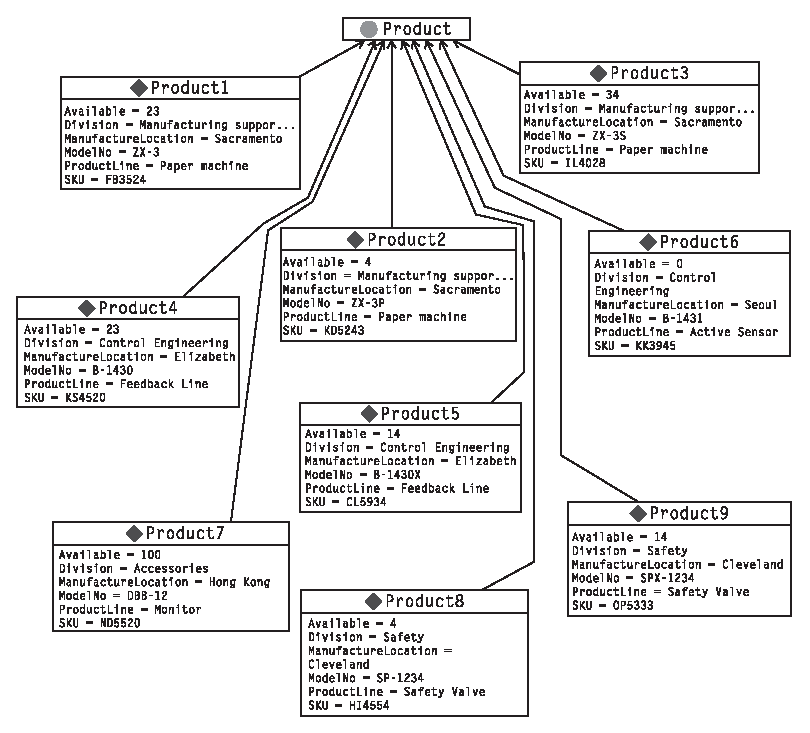
\includegraphics[width=5.0in]{media/ch3/f03-07-9780123859655.eps}
    \caption{Graphical version of the tabular data from Table~\ref{tab:ch3.12}.}
    \label{fig:ch3.7}
\end{figure}


This approach works well for examples like \emph{Shakespeare wrote
Hamlet in 1601}, in which we want to express more information about some
event or statement. It doesn't work so well in cases like
\emph{Wikipedia says Shakespeare wrote Hamlet}, in which we are
expressing information about the statement itself, \emph{Shakespeare
wrote Hamlet}. This kind of metadata about statements often takes the
form of provenance (information about the source of a statement, as in
this example), likelihood (expressed in some quantitative form like
probability, such as \emph{It is 90 percent probable that Shakespeare
wrote Hamlet}), context (specific information about a project setting in
which a statement holds, such as \emph{Kenneth Branagh played Hamlet in
the movie}), or time frame (\emph{Hamlet plays on Broadway January 11
through March 12}). In such cases, it is useful to explicitly make a
statement about a statement. This process, called \emph{explicit reification},
is supported by the W3C RDF standard with three resources called
\texttt{rdf:subject}, \texttt{rdf:predicate}, and \texttt{rdf:object}.

Let's take the example of \emph{Wikipedia says Shakespeare wrote
Hamlet}. Using the RDF standard, we can refer to a triple as follows:

\phantom{I}

\begin{tabular}{|lll|}
\hline
Subject&Predicate&Object\\
\hline
q:n1&rdf:subject&lit:Shakespeare \\
q:n1&rdf:predicate&lit:wrote \\
q:n1&rdf:object&lit:Hamlet \\
\hline
\end{tabular}

\phantom{I}

Then we can express the relation of Wikipedia to this statement as
follows:

\phantom{I}

\begin{tabular}{|lll|}
\hline
Subject&Predicate&Object\\
\hline
web:Wikipedia&m:says&q:n1.\\
\hline
\end{tabular}

\phantom{I}

Notice that just because we have asserted the reification triples about
\texttt{q:n1}, it is not necessarily the case that we have also asserted the
triple itself:

\phantom{I}

\begin{tabular}{|lll|}
\hline
Subject&Predicate&Object\\
\hline
lit:Shakespeare&lit:wrote&lit:Hamlet \\
\hline
\end{tabular}

\phantom{I}

This is as it should be; after all, if an application does not trust
information from Wikipedia, then it should not behave as though that
triple has been asserted. An application that does trust Wikipedia will
want to behave as though it had.


\section{Naming RDF Graphs}
So far, we have seen how a collection of triples can be considered as a graph,
either for display purposes (as in many of the figures in this chapter), or as we will
see in Chapter~\ref{ch6}, for querying.  But we haven't been very
specific about what exactly we mean by a \emph{graph}.

Informally, a graph is a diagram with nodes and edges.  In RDF, this
corresponds directly to a set of triples.  When the same URI is used in
many triples (as in, for example, Figure~\ref{fig:ch3.7}), the drawing
of the graph is be highly connected.

From a more formal point of view in RDF, a graph is simply a set of
triples. They might be highly connect, or not at all, it doesn't
matter; a graph is just a set of triples.

When we manage data sets, we might just refer to all the triples in
our data, as we have done with all the examples in this chapter so
far.  For most situations, this is fine.  But we might want to single
out a set of triples (i.e., a graph) and give \emph{that} a name.
Since this is the web, that name will be in the form of a URI.  The
RDF standard provides a means for doing this - it is called the
\emph{named graph}.

The idea of a named graph is quite simple; we refer to a set of
triples with a name, which itself is a URI. 

Why would we want to name a graph?  There are a few basic use cases:

\begin{itemize}
    \item \emph{One file, one graph.} So far, we have seen examples of how we can 
    extract RDF data from spreadsheets.  We can extract RDF data from other sources as well, 
    and indeed, we can create data natively as RDF.  In the next section, we'll see how 
    to write down RDF data into a plain text file.  When we load this data into an RDF data store, we might want to keep data from different sources separate.  A convenient way to do this is to put all the data from one source into a single named graph.  The name of the graph (as a URI) can even give information as to where we can find that source.
    \item \emph{Reification} In Section~\ref{ch5.reification}, we saw the need for higher-order relationships, in which we want to make statements about statements.  Named graphs provide another way to accomplish this.  We put a set of triples about which we want to make some statement into a named graph, and make the statement about that graph.
    \item \emph{Context} Sometimes when we have a set of triples, we would like to consider them in some context; for example, earlier we considered the fact \emph{Kenneth Brannagh played Hamlet in the movie}.  In this example, \emph{in the movie} (where by \emph{the movie} we are referring specifically to \texttt{https://www.imdb.com/title/tt0116477/}) represents a context for the assertion \emph{Kenneth Brannagh played Hamlet}. 
\end{itemize}

As an example of reification with named graphs, let's return to the statement, \emph{Wikipedia says Shakespeare wrote Hamlet}.   Suppose we start with the single triple stating that fact:

\begin{tabular}{|lll|}
\hline
Subject&Predicate&Object\\
\hline
lit:Shakespeare&lit:wrote&lit:Hamlet \\
\hline
\end{tabular}

Now, let's add a column to this table to specify which named graph this is in.  Furthermore, 
we'll just use the URI \texttt{https://www.wikipedia.org/} for wikipedia (since that's the 
URL for wikipedia itself).  Then we have 

\begin{tabular}{|llll|}
\hline
Subject&Predicate&Object&Graph\\
\hline
lit:Shakespeare&lit:wrote&lit:Hamlet&https://www.wikipedia.org/ \\
\hline
\end{tabular}


This is a bit of a degenerate example, since we have a graph that contains a single triple, 
but there is no reason not to have graphs this small.  Of course, there are a lot of other 
facts that are in the wikipedia graph.  In fact, there is a resource on the web called \texttt{dbpedia} that
does just this - it makes all the data of wikipedia available as RDF data.  We describe it in 
detail in Chapter~\ref{ch5}.


Named graphs are a simple extension to the RDF formalism, and really don't change any of the basics; 
RDF still links one named resource to another, where each name is global in scope (i.e., on the web). 
Named graphs simply allow us to manage sets of these links, and to name them as well.  Sometimes when
we are using named graphs, we refer to \emph{quads} instead of triples; this is because it is possible
to represent a triple and its graph as a four-tuple (as shown in the table above).  The name of the 
fourth entry in the quad is usually called the graph (as it is here), but is sometimes referred to as 
the \emph{context}, anticipating a particular use for the named graph. 

\section{Alternatives for Serialization}
\label{serialization}
So far, we have expressed RDF triples in subject/predicate/object
tabular form or as graphs of boxes and arrows. Although these are simple
and apparent forms to display triples, they aren't always the most
compact forms, or even the most human-friendly form, to see the
relations between entities.

The issue of representing RDF in text doesn't only arise in books and
documents about RDF; it also arises when we want to publish data in RDF
on the Web. In response to this need, there are multiple ways of
expressing RDF in textual form.

One might wonder why we have so many different ways to express RDF, and how they 
differ.  It is useful to compare different serializations to different ways to write
the same language; in English and other European languages, the same sentence can be printed
or written in cursive script.  These don't look at all alike, and there are good reasons
for why we might use one instead of the other in any particular situation.   But we can copy 
a message from cursive to print without any loss of content.  The same is true with the serializations; 
we can express the same triples in one serialization or the other, depending on taste, expediency, 
availability of tools, etc. 

\subsection{N-Triples}
\label{ntriples}

The simplest form is called \emph{N-Triples} and corresponds most directly to
the raw RDF triples. It refers to resources using their fully
unabbreviated URIs. Each URI is written between angle brackets
(\textless{} and \textgreater{}). Three resources are expressed in
subject/predicate/object order, followed by a period (.). For example,
if the namespace mfg corresponds to
\emph{http://www.WorkingOntologist.org/Examples/Chapter3/Manufacture\#}, then the first triple from Table~\ref{tab:ch3.14} is written
in N-Triples as follows:


\begin{lstlisting}
 <http://www.WorkingOntologist.org/Examples/Chapter3/Manufacture#Product1>
 <http://www.w3.org/1999/02/22-rdf-syntax-ns#type> <http://www.WorkingOntologist.org/Examples/Chapter3/Manufacture#Product> .
\end{lstlisting}

It is difficult to print N-Triples on a page in a book---the
serialization does not allow for new lines within a triple (as we had to
do here, to fit it in the page). An actual ntriple file has the whole
triple on a single line. The advantages of N-Triples are that they are
easy to read from a file (parse) and to write into a file for importing
and exporting.

\subsection{Turtle/N3}
\label{ch3.turtle}
In this book, we use a more compact serialization of RDF called
\emph{Turtle} which is itself a subset of a syntax called \emph{N3}. Turtle
combines the apparent display of triples from N-Triples with the
terseness of CURIEs. We will introduce Turtle in this section and
describe just the subset required for the current examples. We will
describe more of the language as needed for later examples. For a full
description of Turtle, see the W3C Recommendation. \cite{Carothers:14:RT}

Since Turtle uses CURIEs, there must be a binding between the (local)
CURIEs and the (global) URIs. Hence, Turtle begins with a preamble in
which these bindings are defined; for example, we can define the CURIEs
needed in the Challenge example with the following preamble:

\begin{lstlisting}
@prefix mfg: <http://www.WorkingOntologist.com/Examples/Chapter3/Manufacturing#>
@prefix rdf: <http://www.w3.org/1999/02/22-rdf-syntax-ns> 
\end{lstlisting}

Once the local CURIEs have been defined, Turtle provides a  simple
way to express a triple by listing three resources, using CURIE
abbreviations, in subject/predicate/object order, followed by a period,
such as the following:

\begin{lstlisting}
mfg:Product1 rdf:type mfg:Product .
\end{lstlisting}

The final period can come directly after the resource for the object,
but we often put a space in front of it, to make it stand out visually.
This space is optional.

It is quite common (especially after importing tabular data) to have
several triples that share a common subject. Turtle provides for a
compact representation of such data. It begins with the first triple in
subject/predicate/object order, as before; but instead of terminating
with a period, it uses a semicolon (;) to indicate that another triple
with the same subject follows. For that triple, only the predicate and
object need to be specified (since it is the same subject from before).
The information in Tables~\ref{tab:ch3.13} and \ref{tab:ch3.14} about \texttt{Product1} and \texttt{Product2}
appears in Turtle as follows:

\begin{lstlisting}
mfg:Product1 rdf:type mfg:Product;
             mfg:Product_Division "Manufacturing support"; 
             mfg:Product_ID "1";
	     mfg:Product_Manufacture_Location "Sacramento";
	     mfg:Product_ModelNo "ZX-3"; 
	     mfg:Product_Product_Line "Paper Machine"; 
	     mfg:Product_SKU "FB3524";
	     mfg:Product_Available "23" .

mfg:Product2 rdf:type mfg:Product; 
             mfg:Product_Division "Manufacturing support"; 
	     mfg:Product_ID "2"; 
	     mfg:Product_Manufacture_Location "Sacramento"; 
	     mfg:Product_ModelNo "ZX-3P"; 
 	     mfg:Product_Product_Line "Paper Machine"; 
	     mfg:Product_SKU "KD5243";
	     mfg:Product_Available "4" .
\end{lstlisting}

When there are several triples that share both subject and predicate,
Turtle provides a compact way to express this as well so that neither
the subject nor the predicate needs to be repeated. Turtle uses a comma
(,) to separate the objects. So the fact that Shakespeare had three
children named Susanna, Judith, and Hamnet can be expressed as follows:

\begin{lstlisting}
lit:Shakespeare b:hasChild b:Susanna, b:Judith, b:Hamnet .
\end{lstlisting}

There are actually three triples represented here---namely:

\begin{lstlisting}
lit:Shakespeare b:hasChild b:Susanna . 
lit:Shakespeare b:hasChild b:Judith . 
lit:Shakespeare b:hasChild b:Hamnet .
\end{lstlisting}

Turtle provides some abbreviations to improve terseness and readability;
in this book, we use just a few of these. One of the most widely used
abbreviations is to use the word \textbf{\texttt{a}} to mean rdf:type. The motivation for
this is that in common speech, we are likely to say, ``Product1 is a
Product'' or ``Shakespeare is a playwright'' for the triples,

\begin{lstlisting}
mfg:Product1 rdf:type mfg:Product . 
lit:Shakespeare rdf:type lit:Playwright .
\end{lstlisting}

respectively. Thus we will usually write instead:

\begin{lstlisting}
mfg:Product1 a mfg:Product . 
lit:Shakespeare a lit:Playwright .
\end{lstlisting}

\subsection{RDF/XML}

While Turtle is convenient for human consumption and is more compact for
the printed page, many Web infrastructures are accustomed to
representing information in HTML or, more generally, XML. For this
reason, the W3C historically started by recommending the use of an XML
serialization of RDF called RDF/XML. The information about \texttt{Product1} and
\texttt{Product2} just shown looks as follows in RDF/XML. In this example, the
subjects (\texttt{Product1} and \texttt{Product2}) are referenced using the XML attribute
\texttt{rdf:about}; the triples with each of these as subjects appear as
subelements within these definitions. The complete details of the
RDF/XML syntax are beyond the scope of this discussion and can be found in the W3C Recommendation. \cite{Schreiber:14:RXS}

\begin{lstlisting}
<rdf:RDF" 
  xmlns:mfg=http://www.WorkingOntologist.com/Examples/Chapter3/Manufacturing#"
  xmlns:rdf=http://www.w3.org/1999/02/22-rdf-syntax- ns#">
<mfg:Product rdf:about="http://www.WorkingOntologist.com/Examples/Chapter3/Manufacturing#Product1">
  <mfg:Available>23</mfg:Available>
  <mfg:Division>Manufacturing support</mfg:Division>
  <mfg:ProductLine>Paper machine</mfg:ProductLine>
  <mfg:SKU>FB3524</mfg:SKU>
  <mfg:ModelNo>ZX-3</mfg:ModelNo>
  <mfg:ManufactureLocation>Sacramento</mfg:ManufactureLocation>
</mfg:Product>
<mfg:Product rdf:about="http://www.WorkingOntologist.com/Examples/Chapter3/Manufacturing#Product2">
  <mfg:SKU>KD5243</mfg:SKU>
  <mfg:Division>Manufacturing support</mfg:Division>
  <mfg:ManufactureLocation>Sacramento</mfg:ManufactureLocation>
  <mfg:Available>4</mfg:Available>
  <mfg:ModelNo>ZX-3P</mfg:ModelNo>
  <mfg:ProductLine>Paper machine</mfg:ProductLine>
</mfg:Product> 
</rdf:RDF>
\end{lstlisting}

The same information is contained in the RDF/XML form as in the Turtle,
including the declarations of the CURIEs for \emph{mfg:} and \emph{rdf:}. RDF/XML
includes a number of rules for determining the fully qualified URI of a
resource mentioned in an RDF/XML document. These details are quite
involved and will not be used for the examples in this book.

\subsection{JSON-LD}
\label{ch3.JSON}

A more modern way to pass data from one component to another in a Web
application is using \emph{JSON}, the Javascript Object Notation cite{bray2014javascript}. In
order to make linked data in RDF more available to applications that use
JSON, the W3C has recommended JSON-LD, JSON for Linked Data \cite{Kellogg:14:J}. There is a
direct correspondence between JSON-LD and RDF triples, making JSON-LD
another serialization format for RDF.

One of the motivations for having a JSON-based serialization for RDF is
that developers who are accustomed to JSON but are not familiar with
graph data or distributed data can build applications purely in JSON,
which are nevertheless compatible with linked data.

The information about \texttt{Product1} and \texttt{Product2} looks as follows in JSONLD:

\begin{lstlisting}
{
  "@graph" : [ {
    "@id" : "mfg:Product1",
    "@type" : "mfg:Product",
    "mfg:Available" : "23",
    "mfg:Division" : "Manufacturing support",
    "mfg:ManufactureLocation" : "Sacramento",
    "mfg:ModelNo" : "ZX-3",
    "mfg:ProductLine" : "Paper machine",
    "mfg:SKU" : "FB3524"
  }, {
    "@id" : "mfg:Product2",
    "@type" : "mfg:Product",
    "mfg:Available" : "4",
    "mfg:Division" : "Manufacturing support",
    "mfg:ManufactureLocation" : "Sacramento",
    "mfg:ModelNo" : "ZX-3P",
    "mfg:ProductLine" : "Paper machine",
    "mfg:SKU" : "KD5243"
  } ],
  "@context" : {
    "rdf" : "http://www.w3.org/1999/02/22-rdf-syntax-ns#",
    "mfg" : "http://www.workingontologist.com/Examples/Chapter3/Manufacturing#"
  }
}
\end{lstlisting}


The document is organized as a \texttt{@graph} and a \texttt{@context}; the context
is like the prefix declarations in Turtle, in that it defines namespaces
abbreviations and their expansions. The graph section describes the
data, organizing it into object structures as much as possible. Each
object has an \texttt{@id}, which defines the URI of the resource (in triple
terms, the subject of each triple). The rest of the object structure is
in the same form as a JSON object, with the fields corresponding to
predicates and the values corresponding to objects.

Optionally, each object can have a \texttt{@type} declaration, which corresponds
to the \texttt{rdf:type} predicate in triples. In this case, the value is
expected to be another resource, and is interpreted as such.

JSON-LD has a provision for referring to other objects as well, by using
a JSON Object syntax, specifying the identity of a referred object with
\texttt{@id}. So, if we were to say that \texttt{Product1} is a part of \texttt{Product2}, we could
say

\begin{lstlisting}
{
  "@graph" : [ {
     @id" : "mfg:Product1",
     "mfg:partOf" : { "@id" : "mfg:Product2" }
  } ]
}    
\end{lstlisting}

JSON-LD provides a valuable way to exchange graph data from one
application to another, while staying entirely in a conventional
Javascript environment. Its consistency with RDF allows these
applications to smoothly integrate into a web of distributed data.

\section{BLANK NODES\label{blanknodes}}

So far, we have described how RDF can represent sets of triples, in
which each subject, predicate, and object is either a source or (in the
case of the object of a triple) a literal data value. Each resource is
given an identity according to the Web standard for identity, the URI.
RDF also allows for resources that do not have any Web identity at all.
But why would we want to represent a resource that has no identity on
the Web?

Sometimes we know that something exists, and we even know some things
about it, but we don't know its identity. For instance, suppose we want
to represent the fact that Shakespeare had a mistress, whose identity
remains unknown. But we know a few things about her; she was a woman,
she lived in England, and she was the inspiration for \emph{Sonnet 78}.

It is simple enough to express these statements in RDF, but we need an
identifier for the mistress. In
Turtle, we could express them as follows:

\begin{lstlisting}
lit:Mistress1 rdf:type bio:Woman;
bio:LivedIn geo:England.
lit:Sonnet78 lit:hasInspiration lit:Mistress1.
\end{lstlisting}

But if we don't want to have an identifier for the mistress, how can we
proceed? RDF allows for a \emph{blank node}, or \emph{bnode} for short, for such a
situation. If we were to indicate a bnode with a ?, the triples would
look as follows:

\begin{lstlisting}
? rdf:type bio:Woman;
  bio:livedIn geo:England. 
lit:Sonnet78 lit:hasInspiration ?.
\end{lstlisting}

The use of the bnode in RDF can essentially be interpreted as a logical
statement, ``there exists.'' That is, in these statements we assert
``there exists a woman, who lived in England, who was the inspiration
for `Sonnet78.'''

But this notation (which does not constitute a valid Turtle expression)
has a problem: If there is
more than one blank node, how do we know which \texttt{?} references which
node? For this reason, Turtle instead includes a compact and unambiguous
notation for describing blank nodes. A blank node is indicated by
putting all the triples of which it is a subject between square brackets
({[} and {]}), so:

\begin{lstlisting}
[ rdf:type bio:Woman;
  bio:livedIn geo:England ]
\end{lstlisting}

It is customary, though not required, to leave blank space after the
opening bracket to indicate that we are acting as if there were a
subject for these triples, even though none is specified.

We can refer to this blank node in other triples by including the entire
bracketed sequence in place of the blank node. Furthermore, the
abbreviation of \texttt{a} for \texttt{rdf:type} is particularly useful in this
context. Thus, our entire statement about the mistress who inspired
``Sonnet 78'' looks as follows in Turtle:

\begin{lstlisting}
lit:Sonnet78 lit:hasInspiration [a :Woman;
             bio:livedIn geo:England].
\end{lstlisting}

This expression of RDF can be read almost directly as plain English:
that is, ``Sonnet78 has {[}as{]} inspiration a Woman {[}who{]} lived in
England.'' The identity of the woman is indeterminate. The use of the
bracket notation for blank nodes will become particularly important when
we come to describe OWL, the Web Ontology Language, since it makes very
particular use of bnodes. While RDF allows for the use of blank nodes in
many circumstances, other than the specific use of blank nodes in OWL,
their use is discouraged in general.

\subsection{Ordered information in RDF\label{ordered}}

The children of Shakespeare appear in a certain order on the printed
page, but from the point of view of RDF, they are in no order at all;
there are just three triples, one describing the relationship between
Shakespeare and each of his children. What if we do want to specify an
ordering. How would we do it in RDF?

RDF provides a facility for ordering elements in a list format. An
ordered list can be expressed quite easily in Turtle as follows:

\begin{lstlisting}
lit:Shakespeare b:hasChild (b:Susanna b:Judith b:Hamnet).
\end{lstlisting}

This translates into the following triples, where \texttt{\_:a}, \texttt{\_:b}, and \texttt{\_:c}
are bnodes, and the order is indicated using two reserved properties in RDF called \texttt{rdf:first} and 
\texttt{rdf:rest}.  The list is terminated with a reference to the resource \texttt{rdf:nil}:

\begin{lstlisting}
lit:Shakespeare b:hasChild _:a.
_:a rdf:first b:Susanna.
_:a rdf:rest _:b.
_:b rdf:first b:Judith.
_:b rdf:rest _:c.
_:c rdf:rest rdf:nil.
_:c rdf:first b:Hamnet.
\end{lstlisting}

This rendition preserves the ordering of the objects but at a cost of
considerable complexity of representation. Fortunately, the Turtle
representation is quite compact, so it is not usually necessary to
remember the details of the RDF triples behind it.

\subsection{N-Quads}

So far, we have talked about how to serialize triples.  But what if we want to 
serialize triples in the context of one or more named graphs?   The W3C provides simple
extensions of the serializations for triples for use with named graphs.  The simplest is
called \emph{N-Quads}. 

Like N-Triples, N-Quads uses no CURIEs and no prefixes.  A triple is written in the form of a 
quad, that is, with Subject, Predicate, Object and Graph, in that order.  So, to extend our example from 
N-Triples, if we were to say that Product1 is a Product in graph \texttt{http://www.WorkingOntologist.org/Examples/Chapter3/Manufacture}, we would simply write

\begin{lstlisting}
<http://www.WorkingOntologist.org/Examples/Chapter3/Manufacture#Product1>
 <http://www.w3.org/1999/02/22-rdf-syntax-ns#type> <http://www.WorkingOntologist.org/Examples/Chapter3/Manufacture#Product> 
 <http://www.WorkingOntologist.org/Examples/Chapter3/Manufacture> .
\end{lstlisting}

This is a very long line indeed (even longer than it was in N-Triples), so it doesn't show up well
in a book, but it is simple to write an parse - no shortcuts, no prefixes, just subject, predicate, object, graph, period. 

\subsection{TriG}
TriG is an extension of the Turtle format from Section~\ref{ch3.turtle}.  It includes all of the
abbreviations for namespaces and elisions with semicolons and commas as Turtle does.  The main difference is 
that it is possible to specify a URI for a graph for all triples in the file.  This is done simply by 
putting all the triples in a graph between braces (\{ and \}), and then prefix the name of the graph. 

For example, if we take the 
example from Section~\ref{ch3.turtle} about manufacturing products, and put them into a graph with name \texttt{<http://www.WorkingOntologist.org/Examples/Chapter3/Manufacture>}, this can be expressed in TriG as follows: 


\begin{lstlisting}
<http://www.WorkingOntologist.org/Examples/Chapter3/Manufacture> 
   { mfg:Product1 rdf:type mfg:Product;
                 mfg:Product_Division "Manufacturing support"; 
                 mfg:Product_ID "1";
                 mfg:Product_Manufacture_Location "Sacramento";
                 mfg:Product_ModelNo "ZX-3"; 
                 mfg:Product_Product_Line "Paper Machine"; 
                 mfg:Product_SKU "FB3524";
                 mfg:Product_Available "23" .
    
    mfg:Product2 rdf:type mfg:Product; 
                 mfg:Product_Division "Manufacturing support"; 
                 mfg:Product_ID "2"; 
                 mfg:Product_Manufacture_Location "Sacramento"; 
                 mfg:Product_ModelNo "ZX-3P"; 
                 mfg:Product_Product_Line "Paper Machine"; 
                 mfg:Product_SKU "KD5243";
                 mfg:Product_Available "4" .
   }
\end{lstlisting}

In this way, we can express several graphs in a single file. 




\section{SUMMARY}


RDF is a simple standard; its job is to model distributed data on the web.
It accomplishes this job, and nothing more.  If you want to model data in a
distributed way,  you can either use RDF or you will re-invent it; there isn't very
much to it.  The basic idea of RDF is that, in a distributed setting, you need a global 
identifier for anything you refer to.  If you want to connect that to some other 
thing, you will need a name for that.  And if you want to connect them, you'll need a
name for the connection.  All of these names have to be global. 

The hypertext web has already given us the global identifiers; we'll see the details of how
the Web infrastructure processes these identifier, but that isn't part of the Semantic Web, that's
part of the Web we all use every day.  RDF doesn't solve the distributed identity problem; the Web solved that,
and RDF re-uses that solution. 

Given this, the very minimum required for distributed represenation of data on the
Web is a way to connect one Web identifier (that is, a URI) to another, with a link that is also named with a URI.  This is the basis of the RDF triple.  Everything else is just plumbing.  If you are distributing data, 
you'll want a way to store it (those are the serializations).  You'll want a way to convert data
from non-distributed forms (like tables) into distributed form.  RDF simply provides the infrastructure to deal
with the simplest way of representing distributed information. 



As a data model, RDF provides a clear specification of what has to
happen to merge information from multiple sources. It does not provide
algorithms or technology to implement those processes. These
technologies are the topic of subsequent chapters.

\subsection{Fundamental concepts}

The following fundamental concepts were introduced in this chapter.

\emph{\textbf{RDF (Resource Description Framework)}}---This distributes
data on the Web.

\emph{\textbf{Triple}}---The fundamental data structure of RDF. A triple
is made up of a subject, predicate, and object.

\emph{\textbf{Graph}}---A nodes-and-links structural view of RDF data.

\emph{\textbf{Merging}}---The process of treating two graphs as if they
were one.

\emph{\textbf{URI (Uniform Resource Indicator)}}---A generalization of
the URL (Uniform Resource Locator), which is the global name on the Web.

\emph{\textbf{namespace}}---A set of names that belongs to a single authority.
Namespaces allow different agents to use the same word in different
ways.

\emph{\textbf{CURIE}}---An abbreviated version of a URI, it is made up of a
namespace identifier and a name, separated by a colon.

\emph{\textbf{rdf:type}}---The relationship between an instance and its type.

\emph{\textbf{rdf:Property}}---The type of any property in RDF.

\emph{\textbf{Reification}}---The practice of making a statement about another
statement. It is done in RDF using

\emph{\textbf{rdf:subject}}, \emph{\textbf{rdf:predicate}}, and \emph{\textbf{rdf:object}}.

\emph{\textbf{N-Triples, Turtle, RDF/XML}}---The serialization syntaxes for
RDF.

\emph{\textbf{Blank nodes}}---RDF nodes that have no URI and thus cannot be
referenced globally. They are used to stand in for anonymous entities.

\chapter{Semantic Web application architecture}
\label{ch4}

So far, we have seen how RDF can represent data in a distributed way
across the Web. As such, it forms the basis for the Semantic Web, a web
of data in which Anyone can say Anything about Any topic. The focus of
this book is modeling on the Semantic Web: describing and defining
distributed data in such a way that the data can be brought back
together in a useful and meaningful way. In a book about only modeling,
one could say that there is no room for a discussion of system
architecture---the components of a computer system that can actually use
these models in useful applications. But this book is for the working
ontologist who builds models so that they can be used. But used for
what? These models are used to build some application that takes
advantage of information distributed over the Web. In short, to put the
Semantic Web to work, we need to describe, at least at a high level, the
structure of a Semantic Web application---in particular, the components
that comprise it, the kinds of inputs it gets (and from where), how it
takes advantage of RDF, and why this is different from other application
architectures.

Many of the components of a Semantic Web application are provided both
as supported products by companies specializing in Semantic Web
technology and as free software under a variety of licenses. New
software is being developed both by research groups as well as product
companies on an ongoing basis. We do not describe any particular tools
in this chapter (W3C has a wiki page listing some tools
\cite{RDFTools}), but instead we discuss the
types of components that make up a Semantic Web deployment and how they
fit together.

\begin{itemize}
\item
  \emph{\textbf{RDF Parser/Serializer:}} We have already seen a number
  of serializations of RDF. An RDF parser reads text in one (or more) of these formats and
  interprets it as triples in the RDF data model. An RDF serializer does the reverse; it takes a set of triples and
creates a file that expresses that content in one of the serialization
forms.
\item
  \emph{\textbf{RDF Store:}} We have seen how RDF distributes data in
  the form of triples. An RDF store (sometimes called a triple store) is
  a database that is tuned for storing and retrieving data in the form
  of triples. In addition to the familiar functions of any database, an
  RDF store has the additional ability to merge information from
  multiple data sources, as defined by the RDF standard.
\item
  \emph{\textbf{RDF Query Engine:}} Closely related to the RDF store is
  the RDF query engine. The query engine provides the capability to
  retrieve information from an RDF store according to structured
  queries.
\item
  \emph{\textbf{Application:}} An application has some work that it
  performs with the data it processes: analysis, user interaction,
  archiving, and so forth. These capabilities are accomplished using
  some programming language that accesses the RDF store via queries
  (processed with the RDF query engine).
\item
  \emph{\textbf{Reasoning Engine:}} A \emph{reasoner} or \emph{reasoning engine} is closely related to the RDF store or
  query engine and provides the capability to infer logical consequences
  from RDF data and schemata.
\end{itemize}

Most of these components have corresponding components in a familiar
relational data-backed application. The relational database itself
corresponds to the RDF store in that it stores the data. The database
includes a query language with a corresponding query engine for
accessing this data. In both cases, the application itself is written
using a general-purpose programming language that makes queries and
processes their results. The parser/serializer has no direct counterpart
in a relational data- backed system, at least as far as standards go.
There is no standard serialization of a relational database that will
allow it to be imported into a competing relational database system
without a change of semantics. (This is a key advantage of RDF stores
over traditional data stores.)

In the following sections, we examine each of these capabilities in
detail. Since new products in each of these categories are being
developed on an ongoing basis, we describe them generically and do not
refer to specific products.

\section{RDF PARSER/SERIALIZER}

How does an RDF-based system get started? Where do the triples come
from? There are a number of possible answers for this, but the simplest
one is to find them directly on the Web.

Google can find millions of files with the extension .rdf. Any of these
could be a source of data for an RDF application. But these files are
useless unless we have a program that can read them. That program is an
RDF parser. RDF parsers take as their input a file in some RDF format.
Most parsers support all the standard RDF formats outlined in Chapter~\ref{ch3}. 
An RDF parser takes such a file as input and converts it into an
internal representation of the triples that are expressed in that file.
At this point, the triples are stored in the triple store and are
available for all the operations of that store.

The triples at this point could also be serialized back out, either in
the same text form or in another text form. This is done using the
reverse operation of the parser: the serializer. It is possible to take
a ``round-trip'' with triples using a parser and serializer; if you
serialize a set of triples, then you parse the resulting string with a
corresponding parser (e.g., a Turtle parser for a Turtle serialization),
and the result is the same set of triples that the process began with.
Notice that this is not necessarily true if you start with a text file
that represents some triples. Even in a single format, there can be many
distinct files that represent the same set of triples. Thus, it is not,
in general, possible to read in an RDF file,
export it again, and be certain that the resulting file will be
identical (character by character) to the input file.

Parsers and serializers based on the standard representations of RDF are
useful for the systematic processing and archiving of data in RDF. While
there are considerable data available in these formats, even more data
are not already available in RDF. Fortunately, for many common data
formats (e.g., tabular data), it is quite easy to convert these formats
into RDF triples.


\subsection{Other data sources- Relational Databases}

In Challenge~\ref{chal:1}, we saw how to convert a table from a relational
database to RDF. The transformation was simple; we used the first column, along
with the name of the table, to produce the URI for the subject of all the 
triples.  We used the names of the columns, also along with the table 
name, to form the URI of the properties.

But this transformation assumed a lot about the table.  It assumed that the
first column, whose name was \texttt{ID}, was the appropriate column to use
as the ID for the subject.  It assumed that the names of the columns were
appropriate property names.  While these assumptions are pretty likely to 
be true in most situations, they are certainly not guaranteed.  How should we
map tables into RDF in other situations? 

Let's consider the following simple table:

\phantom{I}

\begin{tabular}{|lll|}
\hline
ID&NUM &ttl \\
\hline
\hline
87&2616&Hypertext Transfer Protocol -- HTTP/1.1 \\
88&2396&Uniform Resource Identifiers (URI): Generic Syntax\\
     \hline
\end{tabular}

It may seem ``obvious'' that the first column, \texttt{ID}, should be part
of the identifier of the URI for a row.  But as it happens, this data refers to
some standards by the IETF, and it is in fact the standard number (\texttt{NUM}) that 
uniquely  identifies the entity.   The first column was generated by some database
system as an index to this table only; it has no significance when linking this data
to any other.  It would not just be inconvenient to use this as an identifier, it would be
wrong; this record is known to the rest of the system by its \texttt{NUM}, 
and not by its \texttt{ID}.

Furthermore, the last column, \texttt{ttl}, isn't referring to a semantic web format (Turtle);
this is short for ``title''.  We actually a bibliographic standard called 
the \emph{Dublin Core} (dc for short) that provides terms for standard metadata about
publications, like author, title, etc.  It makes more sense to use that property, than to
make one up called \emph{:ttl}.  

The W3C provides a Recommendation called \emph{R2RML} (Relational To RDF Markup Language)
just for this circumstance.  The job of R2RML is to provide enough information about 
the mapping of a table to RDF that we don't have to second guess any of these things. 

In this simple example, we can express the mapping we just described in R2RML as follows: 

\begin{lstlisting}
:My_Table rdf:type rr:TriplesMap ;
          rr:subjectMap [ rr:template "https://www.ietf.org/rfc/rfc{NUM}.txt" ] ;
          rr:predicateObjectMap [
             rr:predicateMap [ rr:predicate dc:title  ];
             rr:objectMap [ rr:column "ttl" ]
          ] .
\end{lstlisting}

When this mapping is applied to the table, first off the \texttt{rr:subjectMap} 
specifies a template for the URIs of the subjects.  In this case, the URI 
includes information about the organization (the IETF) and what this table is
about  (Requests for Comments, or RFCs).  The template indicates that the second 
column (\texttt{NUM}) is the one to be used to fill in the identifiers. 

The \texttt{rr:predicateObjectMap} specifies two things; one is a column name 
(this is a string, since in a database, a column isn't (yet) a URI), and a predicate. 
The interpretation of this is that the value in the specified column in the input will be 
provided as the value for the specified predicate in the output. 

The whole mapping therefore yields the following two triples (where we use \texttt{ietf:} as 
the prefix for \texttt{https://www.ietf.org/rfc/}):

\begin{lstlisting}
ietf:rfc2616.txt dc:title "Hypertext Transfer Protocol -- HTTP/1.1" .
ietf:rfc2396.txt dc:title "Uniform Resource Identifiers (URI): Generic Syntax" .
\end{lstlisting}

If a relational database has foreign keys, the situation is a bit more complex, since 
in the output, this means that the objects of some triples will themselves be 
URIs, which also have to be specified, but the approach is the same; R2RML provides
a language for defining templates that will be used to map from the original tabular 
data to a particular triple in the output. 



\subsection{Other data sources - Web pages}
\label{webembed}

Another rich
source of data for the Semantic Web can be found in existing web
pages---that is, in HTML pages. Such pages often include structured
information, like contact information, descriptions of events, product
descriptions, publications, opening hours, prices, and so on. This information is 
easily understood by humans, but is difficult to extract as linked
data, unless the pages include some specific data markup.   In Chapter~\ref{ch10} 
we will see a number of systems that make use of data embedded in web pages, including 
the \emph{Open Graph Protocol} of Facebook and \emph{Schema.org}, from a consortium that
includes Google, Microsoft, Yahoo and Yandex.   All such effort require some way to
mark up HTML pages to include structured data, and some converter to extract this data. 

A key capability provided by the ability to embed structured data in web pages is 
called \emph{rich snippets}.  A rich snippet refers to the inclusion of structured
data in the display of a search result.  Figure~\ref{fig:ch4.RS} shows an example of two 
search results, one as a rich snippet (a) and the other as a plain snippet.  Rich snippets
can appear in many contexts, but their use in search results is the most familiar. 
You've probably seen hundreds of rich snippets while shopping, without knowing how
the data for them is managed. 

\begin{figure}
    \centering
    
\includegraphics{SWWOv3/media/ch4/WithRichSnippet.png}
    (a)
    
\includegraphics{SWWOv3/media/ch4/WithoutRichSnippet.png}
    (b)
    \caption{Two search results, one with rich snippets (a) and one without (b). }
    \label{fig:ch4.RS}
\end{figure}

The rich snippet in Figure~\ref{fig:ch4.RS}(a) is produced using data that is encoded in the corresponding 
web page.  For example, if the product on the web page is given by the CURIE \texttt{bnb:Buffalo},  
then we the information needed to show that the item is "In stock" is just 
a single triple

\begin{lstlisting}
bnb:Buffalo  :availability  :InStock .
\end{lstlisting}


In Chapter~\ref{ch10} we examine the details of the Schema.org vocabulary, to 
see exactly how  resources like \texttt{:availability} and \texttt{:InStock} are used. 

There are several ways to embed RDF data into an HTML Web page.  The most commonly used ones
today are \emph{Microdata} (pioneered by Schema.org), RDFa (standardized by the W3C)
and JSON-LD, which we already saw in Section~\ref{ch3.JSON}. 

Both Microdata and RDFa work on a similar principle; we add new elements to an 
HTML page that are meaningful to an RDF converter.  In both cases, the new elements
are meaningless to a Web browser, and are ignored, so regular visitors to the
web page see no change.  But for an application that reads the page with the appropriate
converter, the RDF data is available, and can be used to augment search, to provide
a rich snippet, or for any other use case that can use structured product data.  In 
Chapter~\ref{ch14} we will see how this sort of data can be used to support a comparative
shopping application. 

JSON-LD, as we saw in Section~\ref{ch3.JSON}, is a serialization format for RDF, so 
any number of arbitrary triples can be encoded in JSON-LD.  But JSON-LD is also 
a Web-friendly language, which can be included in Web pages verbatim, allowing Web
authors to include arbitrarily complex data in their pages. The advantage of doing this 
the web page author is that they can make sure that downstream applications
like search engines get an accurate picture of the goods they are advertising. 
The advantage of having a standard format for application developers is that they 
can browse over the whole web, and create data-driven applications (like rich snippets)
that improve the quality of the web experience. 

Since all of these methods create RDF triples, they can be used together or 
separately, to provide bits of data that can link together. 


\section{RDF STORE}

A database is a program that stores data, making them available for
future use. An RDF data storage solution is no different; the RDF data
are kept in a system called an RDF store. It is typical for an RDF data
store to be accompanied by a parser and a serializer to populate the
store and publish information from the store, respectively. Just as is
the case for conventional (e.g., relational) data stores, an RDF store
may also include a query engine, as described in the next section.
Conventional data stores are differentiated based on a variety of
performance features, including the volume of data that can be stored,
the speed with which data can be accessed or updated, and the variety of
query languages supported by the query engine. These features are
equally relevant when applied to an RDF store.

In contrast to a relational data store, an RDF store includes as a
fundamental capability, the ability to merge two data sets together.
Because of the flexible nature of the RDF data model, the specification
of such a merge operation is clearly defined. Each data store represents
a set of RDF triples; a merger of two (or more) data sets is the single
data set that includes all and only the triples from the source data
sets. Any resources with the same URI (regardless of the originating
data source) are considered to be equivalent in the merged data set.
Thus, in addition to the usual means of evaluating a data store, an RDF
store can be evaluated on the efficiency of the merge process.

RDF store implementations range from custom programmed database
solutions to fully supported off-the-shelf products from specialty
vendors. Conceptually, the simplest relational implementation of a
triple store is as a single table with three columns, one each for the
subject, predicate, and object of the triple. Table~\ref{tab:ch3.14} shows some data
about Los Angeles Metro stations, organized in this way.

This representation should look familiar, as it is exactly the
representation we used to introduce
RDF triples in Chapter~\ref{ch3}. Since this fits in a relational database
representation, it can be accessed using conventional relational
database tools such as SQL. An experienced SQL programmer would have no
problem writing a query to answer a question like ``List the dc:title of
every instance of metro:Metro in the table.'' As an implementation
representation, it has a number of apparent problems, including the replication of information in the first column
and the difficulty of building indices around string values like URIs.

\begin{table}[h]
\centering
\begin{tabular}{||l l l ||} 
 \hline
 Subject&Predicate&Object \\ [0.5ex] 
 \hline\hline
metro:item0&rdf:type&metro:Metro \\
metro:item0&dc:title&``Allen Station'' \\
metro:item0&simile:address&``395 N. Allen Av., Pasadena 91106'' \\
metro:item1&rdf:type&metro:Metro \\
metro:item1&dc:title&``Chinatown Station'' \\
metro:item1&simile:address&``901 N. Spring St., Los Angeles 90012--1862'' \\
metro:item2&rdf:type&metro:Metro \\
metro:item2&dc:title&``Del Mar Station'' \\
metro:item2&simile:address&``230 S. Raymond Av., Pasadena 91105--2014'' \\
\hline
\end{tabular}
\caption{Names and Addresses of Los Angeles Metro Stations}
\label{tab:ch3.14}
\end{table}





It is not the purpose of this discussion to go into details of the
possible optimizations of the RDF store. These details are the topic of
the particular (sometimes proprietary) solutions provided by a vendor of
an off-the-shelf RDF store. In particular, the issue of building indices
that work on URIs can be solved with a number of well-understood data
organization algorithms. Serious providers of RDF stores differentiate
their offerings based on the scalability and efficiency of these
indexing solutions.

\subsection{RDF data standards and interoperability of RDF stores}

RDF stores bear considerable similarity to relational stores, especially
in terms of how the quality of a store is evaluated. A notable
distinction of RDF stores results from the standardization of the RDF
data model and RDF/XML serialization syntax. Several competing vendors
of relational data stores dominate the market today, and they have for
several decades. While each of these products is based on the same basic
idea of the relational algebra for data representation, it is a
difficult process to transfer a whole database from one system to
another. That is, there is no standard serialization language with which
one can completely describe a relational database in such a way that it
can be automatically imported into a competitor's system. Such a task is
possible, but it typically requires a database programmer to track down
the particulars of the source database to ensure that they are
represented faithfully in the target system.

The standardization effort for RDF makes the situation very different
when it comes to RDF stores. Just as for relational stores, there are
several competing vendors and projects. In stark contrast to the
situation for relational databases, the underlying RDF data model is
shared by all of these products, and, even more specifically, all of
them can import and export their data sets in any of the standard
formats (RDF/XML,Turtle, JSON-LD, N3, etc. ). This makes it a routine
task to transfer an RDF data set---or several RDF data sets---from one
RDF store to another. This feature, which is a result of an early and
aggressive standardization process, makes it much easier to begin with
one RDF store, secure in the knowledge that the system can be migrated
to another as the need arises. It also simplifies the issue of
federating data that are housed in multiple RDF stores, possibly coming
from different vendor sources.

\subsection{RDF query engines}

An RDF store is typically accessed using a query language. In this
sense, an RDF store is similar to a relational database or an XML store.
Not surprisingly, in the early days of RDF, a number of different query
languages were available, each supported by some RDF-based product or
open-source project. From the common features of these query languages,
the W3C has undertaken the process of standardizing an RDF query
language called SPARQL. We cover the details of the SPARQL query
language in Chapter~\ref{ch6}.

An RDF query engine is intimately tied to the RDF store. To solve a
query, the engine relies on the indices and internal representations of
the RDF store: the more finely tuned the store is to the query engine,
the better its performance. For large-scale applications, it is
preferable to have an RDF store and query engine that retain their
performance even in the face of very large data sets. For smaller
applications, other features (e.g., cost, ease of installation,
platform, open-source status, and built-in integration with other
enterprise systems) may dominate.

The SPARQL query language includes a protocol for communicating queries
and results so that a query engine can act as a web service. This
provides another source of data for the semantic web--- the so-called
\emph{SPARQL endpoints} provide access to large amounts of structured
RDF data. It is even possible to provide SPARQL access to databases that
are not triple stores, effectively translating SPARQL queries into the
query language of the underlying store. The W3C has recently begun the
process to standardize a translation from SPARQL to SQL for relational
stores.

\subsection{Comparison to relational queries}

In many ways, an RDF query engine is very similar to the query engine in
a relational data store: It provides a standard interface to the data
and defines a formalism by which data are viewed. A relational query
language is based on the relational algebra of joins and foreign key
references. RDF query languages look more like statements in predicate
calculus. Unification variables are used to express constraints between
the patterns.

A relational query describes a new data table that is formed by
combining two or more source tables. An RDF query can describe a new
graph that is formed by describing a subset of a source RDF graph. That
graph, in turn, may be the result of having merged together several
other graphs. The inherently recursive nature of graphs simplifies a
number of detailed issues that arise in table-based queries. For
instance, SPARQL has little need for a subquery construct; in many
cases, the same effect can be achieved with a single query. Similarly,
there is nothing corresponding to the special case of an SQL
``self-join'' in SPARQL.

In the special case in which an RDF store is implemented as a single
table in a relational database, any graph pattern match in such a
scenario will constitute a self-join on that table. Some end- developers
choose to work this way in a familiar SQL environment. Oracle takes
another approach to making RDF queries accessible to SQL programmers by
providing its own SPARQL extension to its version of SQL, optimized for
graph queries. Their SPARQL engine is smoothly integrated with the
table/join structure of their SQL scripting language.

\section{Application Code}

Database applications include more than just a database and query
engine; they also include some application code, in an application
environment, that performs some analysis on or displays some information
from the database. The only access the application has to the database
is through the query interface, as shown in Figure~\ref{fig:ch4.1}.

An RDF application has a similar architecture, but it includes the RDF
parser and serializer, converters, the RDF merge functionality, and the
RDF query engine. These capabilities interact with the application
itself and the RDF store as shown in Figure~\ref{fig:ch4.2}.

The application itself can take any of several forms. Most commonly, it
is written in a conventional programming language (Java, C, Python, and
Perl are popular options). In this case, the RDF capabilities are
provided as API bindings for that language. It is also common for an RDF
store to provide a scripting language as part of the query system, which
gives programmatic access to these capabilities in a way that is not
unlike how advanced dialects of SQL provide scripting capabilities for
relational database applications.

\begin{figure}
    \centering
    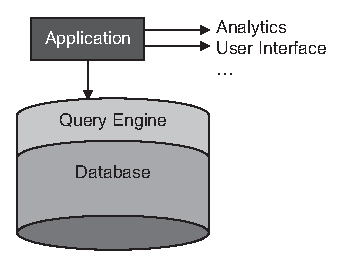
\includegraphics[width=5.0in]{media/ch4/f04-01-9780123859655.eps}
    \caption{Application architecture for a database application.}
    \label{fig:ch4.1}
\end{figure}


\begin{figure}
    \centering
    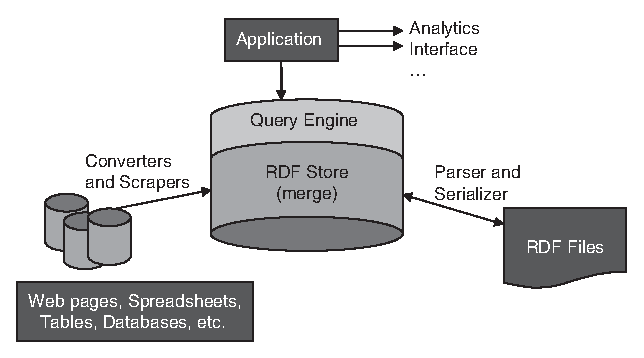
\includegraphics[width=5.0in]{media/ch4/f04-02-9780123859655.eps}
    \caption{Application architecture for an RDF application.}
    \label{fig:ch4.2}
\end{figure}

Regardless of the method by which the RDF store makes these
functionalities available to the application, it is still the
responsibility of the application to use them. Here are some examples of
typical RDF applications:

\begin{itemize}
    \item Calendar integration---shows appointments from different people and
teams on a single calendar view
    \item Map integration---shows locations of points of interest gathered from
different web sites, spreadsheets, and databases all on a single map
    \item Annotation---allows a community of users to apply keywords (with URIs)
to information (tagging) for others to consult
    \item Content management---makes a single index of information resources
(documents, web pages, databases, etc.) that are available in several
content stores.
\end{itemize}

The application will decide what information sources need to be scraped
or converted (e.g., diary entries in XML, lists of addresses from a web
page, directory listings of content servers).

Depending on the volatility of the data, some of this process may even
happen offline (e.g., locations of subway stations in New York, entries
in the Sears catalog, analyses of common chemical structures, etc.,
don't change very rapidly; these sorts of data could be imported into
RDF entirely outside of an application context), whereas other data
(like calendar data of team members, transactional sales data,
experimental results) will have to be updated on a regular basis. Some
data can remain in the RDF store itself (private information about this
team, order information, patented chemical formulas); other data could
be published in RDF form for other applications to use (train
timetables, catalog specials, FDA findings about certain chemicals).

Once all the required data sources have been converted, fetched, or
parsed, the application uses the merge functionality of the RDF store to
produce a single, federated graph of all the merged data. It is this
federated graph that the application will use for all further queries.
There is no need for the queries themselves to be aware of the
federation strategy or schedule; the federation has already taken place
when the RDF merge was performed.

From this point onward, the application behaves very like any other
database application. A web page to display the appointments of any
member of a team will include a query for that information. Even if the
appointments came from different sources and the information about team
membership from still another source, the query is made against the
federated information graph.

\subsection{RDF-backed web portals}

When the front end of an application is a web server, the architecture
(shown in Figure\ref{fig:ch4.1}) is well known for a database-backed web portal.
The pages are generated using any of a number of technologies (e.g.,
CGI, ASP, JSP, React, Angular) that allow web pages to be constructed
from the results of queries against a database. In the earliest days of
the web, web pages were typically stored statically as files in a file
system. The move to database-backed portals was made to allow web sites
to reflect the complex interrelated structure of data as it appears in a
relational database.

The system architecture outlined in Figure~\ref{fig:ch4.2} can be used the same way
to implement a Semantic Web portal. The RDF store plays the same role
that the database plays in database-backed portals. It is important to
note that because of the separation between the presentation layer in
both Figures \ref{fig:ch4.1} and \ref{fig:ch4.2}, it is possible to use all the same 
technologies for the actual web
page construction for a Semantic Web portal as those used in a
database-backed portal. But, in contrast to conventional data-backed web
portals, and because of the distributed nature of the RDF store that
backs a Semantic Web portal, information on a single RDF-backed web page
typically comes from multiple sources. The merge capability of an RDF
store supports this sort of information distribution as part of the
infrastructure of the web portal. When the portal is backed by RDF,
there is no difference between building a distributed web portal and one
in which all the information is local. Using RDF, federated web portals
are as easy as siloed portals.

\section{Data Federation}

The RDF data model was designed from the beginning with data federation
in mind. Information from any source is converted into a set of triples
so that data federation of any kind---spreadsheets and XML, database
tables and web pages---is accomplished with a single mechanism. As shown
in Figure~\ref{fig:ch4.2},

this strategy of federation converts information from multiple sources
into a single format and then combines all the information into a single
store. This is in contrast to a federation strategy in which the
application queries each source using a method corresponding to that
format. RDF does not refer to a file format or a particular language for
encoding data but rather to the data model of representing information
in triples. It is this feature of RDF that allows data to be federated
in this way. The mechanism for merging this information, and the details
of the RDF data model, can be encapsulated into a piece of
software---the RDF store---to be used as a building block for
applications.

The strategy of federating information first and then querying the
federated information store separates the concerns of data federation
from the operational concerns of the application. Queries written in the
application need not know where a particular triple came from. This
allows a single query to seamlessly operate over multiple data sources
without elaborate planning on the part of the query author. This also
means that changes to the application to federate further data sources
will not impact the queries in the application itself.

This feature of RDF applications forms the key to much of the discussion
that follows. In our discussion of RDFS and OWL, we will assume that any
federation necessary for the application has already taken place; that
is, all queries and inferences will take place on the federated graph.
The federated graph is simply the graph that includes information from
all the federated data sources over which application queries will be
run.

\section{Summary}

The components described in this chapter---RDF parsers, serializers,
stores, and query engines---are not semantic models in themselves but
the components of a system that will include semantic models. Even the
information represented in RDF is not necessarily a semantic model.
These are the building blocks that go into making and using a semantic
model. The model will be represented in RDF, to be sure. As we shall
see, the semantic modeling languages of the W3C, RDFS, and OWL are built
entirely in RDF, and they can be federated just like any other RDF data.

Where do semantic models fit into the application architecture of Figure~\ref{fig:ch4.2}? 
As data expressed in
RDF, they will be housed in the RDF store, along with all other data.
But semantic models go beyond just including data that will be used to
answer a query, like the list of plays that Shakespeare wrote or the
places where paper machines are kept. Semantic models also include
meta-data; data that help to organize other data. When we federate
information from multiple sources, the RDF data model allows us to
represent all the data in a single, uniform way. But it does nothing to
resolve any conflicts of meaning between the sources. Do two states have
the same definitions of ``marriage''? Is the notion of ``writing'' a
play the same as the notion of ``writing'' a song? It is the semantic
models that give answers to questions like these. A semantic model acts
as a sort of glue between disparate, federated data sources so we can
describe how they fit together.

Just as Anyone can say Anything about Any topic, so also can anyone say
anything about a model; that is, anyone can contribute to the definition
and mapping between information sources. In this way, not only can a
federated, RDF-based, semantic application get its information from
multiple sources, but it can even get the instructions on how to combine
information from multiple sources. In this way, the Semantic Web really
is a web of meaning, with multiple sources describing what the
information on the Web means.

\subsection{Fundamental concepts}

The following fundamental concepts were introduced in this chapter:

\emph{\textbf{RDF parser/serializer}}---A system component for reading and writing RDF
in one of several file formats.

\emph{\textbf{RDF store}}---A database that works in RDF. One of its main operations is
to merge RDF graphs. RDF query engine---This provides access to an RDF
store, much as an SQL engine provides access to a relational store.

\emph{\textbf{SPARQL}}---The W3C standard query language for RDF.

\emph{\textbf{SPARQL endpoint}}---An application that can answer a SPARQL query,
including one where the native encoding of information is not in RDF.

\emph{\textbf{Application interface}}---The part of the application that uses the
content of an RDF store in an interaction with some user.

\emph{\textbf{Converter}}---A tool that converts data from some form (e.g., tables) into
RDF.

\emph{\textbf{RDFa}}---Standard for encoding and retrieving RDF metadata from HTML
pages.

\chapter{Linked Data}
\label{ch5}
\usepackage{arabtex}
\usepackage{utf8}
\usepackage{CJKutf8}
\section{Weaving a Web of Data}



The architects  of the World Wide Web made some very specific choices in its design 
to allow it to grow to global scale.   The  Web relies on open standards to specify the components of its
architecture, allowing them to span different software and hardware, making it both implementation-independent and domain-independent. To
support a Web of data, we want to take advantage of this infrastructure as much as possible. 
By
reusing  the World Wide Web architecture, the Web of data
becomes a backward-compatible extension and evolution of the hypertext
Web and remains compatible and combinable with all the other facets of
it. The Web of data applies the Web architecture to structured data
sharing on a World Wide scale. Meanwhile, it retains its architectural
support for decentralization, extensibility and openness.


What changes do we have to make to the hypertext Web to allow the Web of data
to be able to describe  resources and publish data? As
shown in Figure~\ref{fig:ch5.1}, this requires two steps:  expanding the set of exchange formats from     HTML (and other document formats) to include  RDF and its serializations (Section~\ref{serialization}) for exchanging data, and generalizing 
URLs (Uniform Resource Locators) to URIs (Uniform Resource Identifiers) 
or IRIs (Internationalized resource identifiers), to identify and then describe virtually anything. ,

\begin{figure}
    \centering
    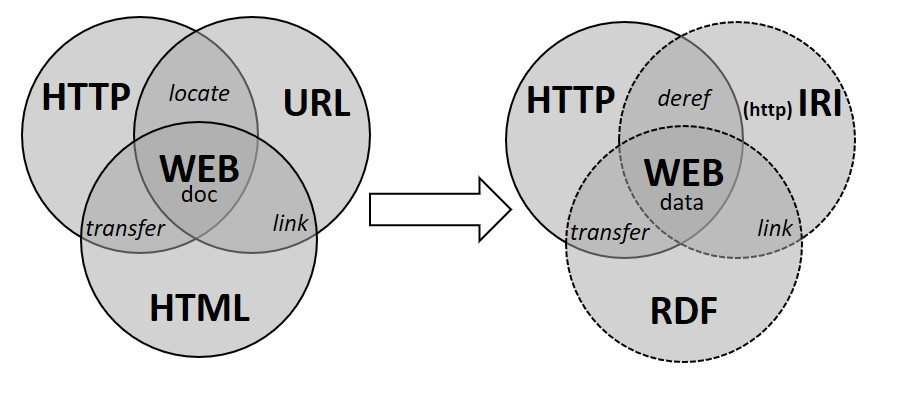
\includegraphics[width=5.0in]{media/ch5/figure-05-01.jpg}
    \caption{Relying on the Web architecture to publish linked data}
    \label{fig:ch5.1}
\end{figure}


Publishing data on the Web is not only about dumping data somewhere on
the Web, it also means linking data so that it can be found, browsed,
crawled, integrated, etc. So in a Web of data, the core idea is the one
of \emph{linked data}, i.e. datasets (and data elements in them)  linked across the
World Wide Web in the same way Web pages, Web sites and anchored texts
are linked across the World on the Web. Instead of just
using HTML to write Web pages that inlcude links to other pages, the Web of
data uses RDF to write data descriptions that include links to other data
descriptions.

Tim Berners-Lee introduced best practices for linked data in his
personal notes on Linked Data Design Issues in 2006\footnote{Linked
  Data, Tim Berners-Lee, 2006-07-27,
  https://www.w3.org/DesignIssues/LinkedData.html}, stating the
architectural principles and explaining the thinking behind the linked data
specifications.   In this chapter, we will explain in detail his three rules 
for data publication that will allow us to weave a web of data:



\begin{enumerate}
\def\labelenumi{\arabic{enumi}.}
\item
\label{ruleURI}
  Use HTTP URIs to name everything: Just as URLs were introduced to
  address and locate resources on the Web, the Web of data uses URIs to
  name the things it describes. But by using HTTP URIs we can also
  provide a default mechanism to obtain descriptions: HTTP URIs are
  names (URIs) supporting lookup (HTTP access). This allow us to
  look up the name of the things they identify.
\item
\label{ruleFYN}
  When an agent accesses an HTTP URI, the server must provide descriptive
  information about the resource identified by that URI using the Web
  standard languages, in particular RDF and its syntaxes.
\item
\label{ruleLink}
  In the descriptive data it provides, a server must include links to
  HTTP URIs of other things so that Web clients can discover more things
  by looking up these new HTTP URIs recursively at will.
\end{enumerate}

These simple rules are a natural extension of how thy hypertext Web works. When we put a hypertext page 
on the web, use an HTTP URI (URL) to reference it.  When an agent accesses that HTTP URI, the server provides 
the page itself.  A hypertext page refers to other pages by including links to their HTTP URIs. 
For the hypertext web, this makes the pages interconnected; from any page an 
information consumer can access others.

By applying these  rules to the Web of data, we make it interconnected in the same way.  
when we use an HTTP URI   for our data elements (rule \ref{ruleURI}), 
we make it possible for anyone on the web to reference them. Once someone
(re-)uses one of our HTTP URIs , their dataset and ours
are interconnected.  When we include links in our data to 
other data sets (rule \ref{ruleLink}) and  describe our own 
datasets (rule \ref{ruleFYN}), we make 
the interconnected data \emph{discoverable}, that is, 
someone coming to one data set can discover another
without having to search for it. 


\hypertarget{calling-a-cat-an-httpcat}{%
\subsection{Calling a cat an
http://cat}\label{calling-a-cat-an-httpcat}}

When we expand the hypertext web into a full Web of data, instead of just using URLs to 
identify what exists on the web (\url{http://my-site.fr}), we also start using
URIs to identify, on the web, what exists in general
(e.g., \url{http://animals.org/cat\#mytsie}, for Fabien's cat, Mytsie).  As we include IRIs in the Web of data, we identify,
on the web, what exists, in any language
(e.g., http://\<الحيوانات.tn/ >.tn/\begin{CJK*}{UTF8}{gbsn}猫
\end{CJK*}\#mytsie).



The distinction between identifying what is on the Web vs. identifying
on the Web anything that exists, is much more than a play on words.
Instead of just using the Web to exchange data about its own content, we
can use it to exchange data about anything around us: a page, a person,
a car, a cat, an idea, a country, a product, a service, a policy, a
relation, etc.

In the acronyms URL, URI and IRI the `R' stands for ``Resource''. In the
Web architecture a resource is anything that can be identified. And in
practice, URIs are now used to name a lot of very different things. Here
are some examples:

\begin{itemize}
\item
  URI for Paris in DBpedia: \url{http://dbpedia.org/resource/Paris}
\item
  URI for the protein MUC18 in UniProt:
  \url{http://www.uniprot.org/uniprot/P43121}
\item
  URI for the name of Victor Hugo in the Library of Congress:
  \url{http://id.loc.gov/authorities/names/n79091479}
\item
  URI for Xavier Dolan in Wikidata:
  \url{http://www.wikidata.org/entity/Q551861}
\item
  URI for Fabien Gandon at Inria:
  \url{http://ns.inria.fr/fabien.gandon\#me}
\item
  URI for the "31st of December 2016 at 23:00 in New York":
  \url{http://www.timeanddate.com/worldclock/meetingdetails.html?year=2017\&month=1\&day=1\&hour=4\&min=0\&sec=0\&p1=179}
\end{itemize}

The reliance on URIs is key to distributed data, to the Web\-based
architecture and to the integration of datasets coming from different
sources and produced by different means.

URIs  allow us to make  vocabulary and  resource
identification unambiguous by providing a global identification
mechanism for the terms and subjects of our descriptions. URIs also have a 
\emph{deferencing} mechanism, that is, a method that uses the URI to find a location 
on the web from which further information can be loaded. 
Applications use this universal
identification mechanism to ensure they are processing the right data,
in the right way and they use the dereferencing mechanism to obtain more
data on demand.

When URIs are used and reused across RDF graphs and datasets, they
provide junction points that allow us to merge the datasets regardless
of their provenance, potentially forming a  giant global graph. This
extensible nature of RDF graphs provides a way to weave a World-Wide Web
of data.

\subsection{Things, Representations and Identifiers}
\label{usehttp}
When we use URLs for Web resources alongside URIs for things, we can
leave our datasets open to some confusion. For example, if we use the
same URI for a cat and for a document about that cat, as soon as we
start attaching descriptions to that URI we need to know precisely what
we are talking about. For instance, if we attach a property to that URI
to provide a ``size'' it is important to know if it refers to the size of the
cat or the size of the document about the cat. For this reason, the best
practice is to use different URIs to identify different resources, and
to realize that a cat and a document about that cat (or a picture of
that cat) are not the same thing. Then, relying on the standard
mechanisms of the Web architecture we can learn more about these
different URIs and their link and for instance, as we will see in the
next section, how to obtain the URL of a document about a cat from the
URI identifying that cat (see Figure~\ref{fig:ch5.cats})

\begin{figure}
    \centering
    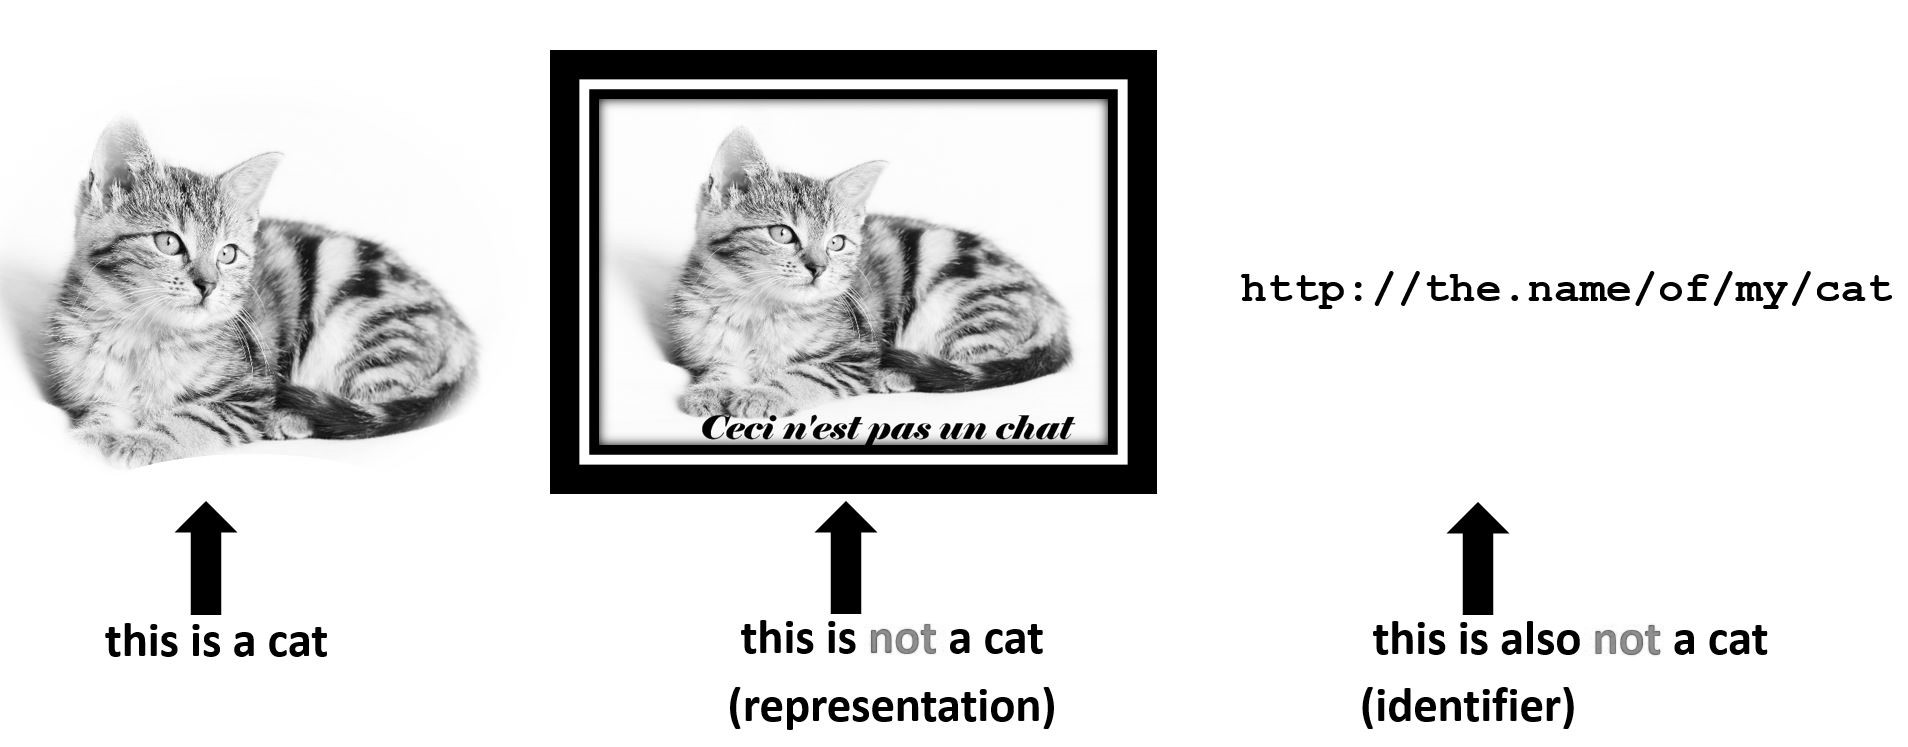
\includegraphics[width=5in]{media/ch5/WebAndCats.jpg}
    \caption{The difference between a cat, a picture of a cat, and an identifier for that cat.  Good linked data practice suggests using an identifer that can be used to look up the picture. }
    % free for commercial use, see https://pixabay.com/en/cat-pet-striped-kitten-young-1192026/
    \label{fig:ch5.cats}
\end{figure}

\hypertarget{dereferencing-http-uri}{%
\subsection{Dereferencing HTTP URI }\label{dereferencing-http-uri}}

An HTTP URI is a URI created to name anything we want to talk about 
that  uses  HTTP   as its dereferencing mechanism. When a person or a
software agent (e.g. a Web crawler) comes across that URI, they can easily learn more
about the resource it represents,  by simply making an HTTP call
to the address it provides.   Dereferencing of HTTP URIs is a cornerstone of the hypertext web, and has
functioned well since the beginning of the Web. HTTP URIs come with an
obvious way to get a description about the resource they identify: the
HTTP protocol that can be used to looked them up. Other URI schemes
(e.g. URN, DOI, etc.) require additional services or practices to be
dereferenced.  

We don't use the term URL (Uniform Resource \textbf{Locator}) for these identifiers, to emphasize the 
point that the thing  being
represented may not itself be on the Web at this address, or even at on the Web at all. For example, I
may want to specify an HTTP URI for my cat Mytsie. No matter how hard I
try, Mytsie herself will never be located on the Web, so I cannot give
her a URL \emph{per se}. But this adorable cat can be identified on the
Web by an HTTP URI and if you ever go to that address you will be
provided with a description (maybe even a photo or two) on the Web about the resource represented by
that URI, i.e. my cat Mytsie.

This approach to linked data, in which we use an HTTP URI as an identifier, and 
rely on HTTP-based dereferencing of that URI to provide more information about the resource, 
is summarized in a web design pattern called \emph{Follow Your Nose} \footnote{Linked Data Patterns, by Leigh Dodds and Ian Davis,
http://patterns.dataincubator.org/book/follow-your-nose.html}.
According to the  Follow Your Nose pattern,  it is the responsibility of the data publisher
to make sure that the HTTP URIs indeed resolve to web resources that provide
appropriate information. Just as Ariadne provided Theseus a thread to let him
find his way back out of the labyrinth, the web publisher provides HTTP URIs
that allow data consumers to find their way back to the data source, to
learn more about it.  It is up to the data consumer and the details of their application (including issues around performance, trust, scalability,
quality, etc.)
whether they want to follow these links at any particular time. 


Since HTTP URIs rely on the domain names to create the first part of the
URI scheme, they support the decentralized creation of globally unique
identifiers. Any owner of a web domain can create and control the access to
any HTTP URIs in that domain. In choosing and using HTTP URIs, there are
three important standard mechanisms of the Web and Internet to be aware
of: the Domain Name Service (DNS) and its implication on the choice of
domain part of the URIs; content negotiation in HTTP, which allows a
server to serve different contents for the same HTTP URI to different
clients; and HTTP redirection, which allows a server to redirect a call
to another address. These three mechanisms and their impacts are
illustrated in figure~\ref{fig:ch5.2} and detailed in the next sections.



\begin{figure}
    \centering
        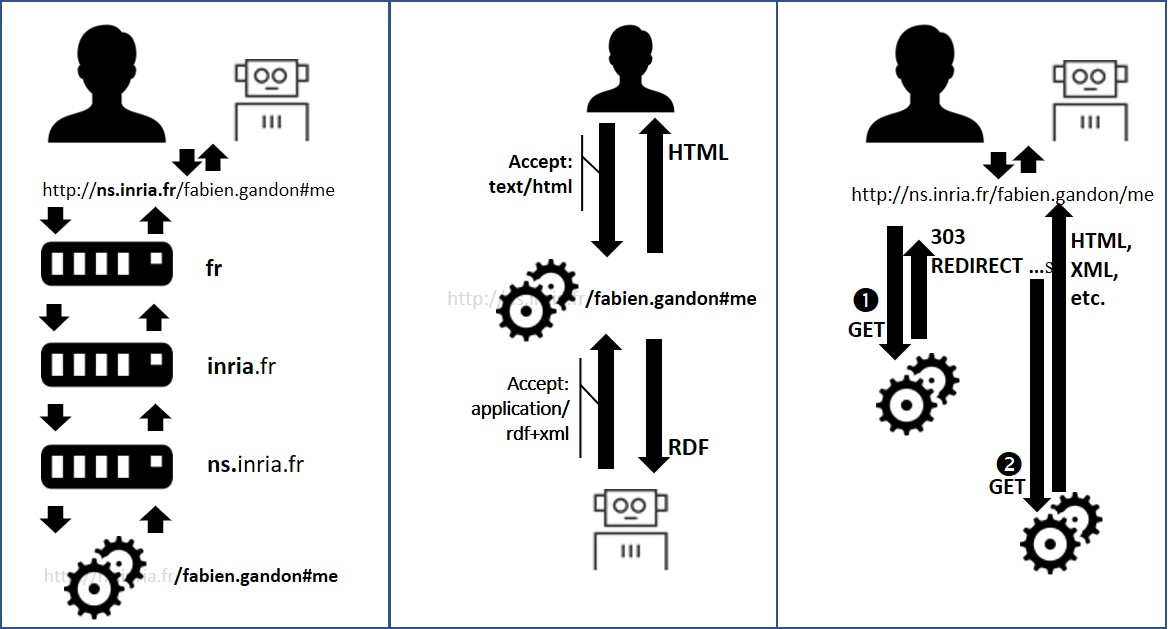
\includegraphics[width=5.0in]{media/ch5/figure-05-02.jpg}
    \caption{Three standard mechanisms used in Web Data publishing and
accessing}
    \label{fig:ch5.2}
\end{figure}


\hypertarget{minting-http-uris}{%
\subsection{Minting HTTP URIs}\label{minting-http-uris}}

How do we choose the URIs we are going to use to talk about the things
we want to describe? What should be their structure or naming schema?
Are there criteria and pitfalls in choosing a method to create URIs for
our collections and applications? These questions are legitimate since
as soon as we start publishing URIs they are reused and referenced and
therefore introduce dependencies and create legacy systems.

The generic form of a URI is describe in their standard
document\footnote{URIs are standardized in RFCs from IETF : RFC 3986
  https://tools.ietf.org/html/rfc3986} like this where values between
square brackets are optional parts one can use in minting a URI (eg.
Indicating a port on a server).

\begin{lstlisting}
scheme:[//[user:password@]host[:port]][/]path[?query][#fragment]
\end{lstlisting}

For instance, a valid URI according to this pattern is for instance:

\begin{lstlisting}
urn:animals.org\#mycat
\end{lstlisting}

As we saw in Section~\ref{usehttp}, using HTTP URIs is preferring for the web 
of data, in contrast to other protocols.  An HTTP URI has the form: 



\begin{lstlisting}
http://host[:port]][/]path[?query][#fragment]
\end{lstlisting}


For instance, the following are valid HTTP URIs:

\begin{lstlisting}
http://animals.org#mycat
http://animals.org/cats/mine
http://animals.org/cats/?owner=fabien
...
\end{lstlisting}


Within a single domain (which corresponds to the \emph{host} in the HTTP protocol, 
the \emph{path} part of the HTTP URI can be arbitrarily long, therefore. 
no practical limit on the number of possible URI patterns we have at our disposal to name the things we
want to describe on the Web. 

\subsetcion{How to build a URI}

Since we are using HTTP URIs for all our data elements, we need to have some 
method for how we will generate enough distinct URIs for everything we want to describe in our data. 
The problem of coming up with appropriate identifiers in a large data set is not 
specific to the Semantic Web, and there is no perfect answer. In the context of HTTP URIs for the Semantic Web,
Pros
and Cons have been discussed in several places\footnote{Cool URIS:
  \url{http://www.w3.org/TR/cooluris/} and Issue 57:
  \url{http://www.w3.org/2001/tag/awwsw/issue57/latest/}}.  We will
summarize here some of the things to consider when minting your HTTP
URIs. 


Inspired by the title of an article by Tim Berners-Lee, \emph{Cool URIs don't change}, \footnote{Cool URIs don't change, Tim Berners-Lee, 1998.  http://www.w3.org/Provider/Style/URI.}, a popular proposal for 
minting URIs for the semantic Web is called \emph{Cool URIs}

As suggested by the eponymous article, a key aspect of cool URIs is that they don't change: you want to ensure
that your URIs will be as stable as possible by choosing a stable URI pattern. 
Why is it important to have stable URIs?  
While the ``404 page not found'' error is disappointing on the hypertext web, it can be catastrophic in the Web of Data, wherethe URIs are the
linkage points between data sets.  A broken link can mean loss of access to an entire data set.

The Cool URI proposal has some advice for how to make URIs stable:

\begin{itemize}
    \item Desing URIs with reference to as few implementation details as possible. In particular, avoid language dependent extensions (.PHP, .json, .rdf), specific server names "desktop8.inria.fr", specific software (\ldots{}/wordpress/\ldots{}), server port number, etc.  
    \item Web servers are able to negotiate content based on information from web clients. Use this feature to avoid implementation details in URIs.
    \item Leave out version information from stable URIs.  The semantic web standards provide ways to specify the version of a data or metadata set, other than changing URIs. 
    \item in many cases, the original data source has some kind of identifier already (a primary key, or an account number, etc.).  You can make use of these to ensure that your URIs correspond to the right data elements. 
\end{itemize}



For example, imagine  we have a table of animals (e.g. a CSV file) with columns
providing information about the vaccination records for our pets, as shown in Table~\ref{tab:ch5.pets}

\begin{table}
    \centering
    \begin{tabular}{|l l l l|}
    \hline
    ID&Species&Name&Expiration Date \\
    \hline\hline
366863&dog&Fido&2020 \\
851903&dog&Bastian&2021 \\
775304&cat&Mytsie&2019 \\
898202&cat&Corvus&2021 \\
847823&cat&Fenris&2019 \\
399378&dog&Maddie&2022 \\
911236&cat&Twinkie&2016 \\
897991&dog&Champ&2019 \\
032579&dog&Zeke&2020 \\
31450&cat&Nix&2019 \\
87580&dog&Fido&2021 \\
\hline
    \end{tabular}
    \caption{Sample data about the vaccine records for our pets. }
    \label{tab:ch5.pets}
\end{table}


The data about the Pet's name and the expiration date of the vaccine cannot be counted on to be  unique
(in this short sample, we have two dogs named Fido).  One option for minting URIs for this would be to include all the data in each URI, as in Table~\ref{tab:ch5.all}.

This method is guaranteed to ensure uniqueness in the data, but makes for very long URIs, and can be misleading if any of the data changes.  Should we coin new URIs?  Or re-use the old ones, which will then reflect out-of-date data?

\begin{table}
    \centering
    \begin{tabular}{|l|}
    \hline
    URI \\
    \hline\hline
http://www.example.com/vac/366863/dog/Fido/2020 \\
http://www.example.com/vac/851903/dog/Bastian/2021 \\
http://www.example.com/vac/775304/cat/Mytsie/2019 \\
http://www.example.com/vac/898202/cat/Corvus/2021 \\
http://www.example.com/vac/847823/cat/Fenris/2019 \\
http://www.example.com/vac/399378/dog/Maddie/2022 \\
http://www.example.com/vac/911236/cat/Twinkie/2016 \\
http://www.example.com/vac/897991/dog/Champ/2019 \\
http://www.example.com/vac/032579/dog/Zeke/2020 \\
http://www.example.com/vac/31450/cat/Nix/2019 \\
http://www.example.com/vac/87580/dog/Fido/2021 \\
\hline
    \end{tabular}
    \caption{Coining URIs by repeating all the data }
    \label{tab:ch5.all}
\end{table}

Since the original data includes an \textbf{ID} field, we can rest assured that this 
will uniquely identify a vaccination, so we can use it for the URI, as in Table~\ref{ch5.id}

\begin{table}
    \centering
    \begin{tabular}{|l |}
    \hline
    URI \\
    \hline\hline
http://www.example.com/vac/366863 \\
http://www.example.com/vac/851903 \\
http://www.example.com/vac/775304 \\
http://www.example.com/vac/898202 \\
http://www.example.com/vac/847823 \\
http://www.example.com/vac/399378 \\
http://www.example.com/vac/911236 \\
http://www.example.com/vac/897991 \\
http://www.example.com/vac/032579 \\
http://www.example.com/vac/31450 \\
http://www.example.com/vac/87580 \\
\hline
    \end{tabular}
    \caption{Coining URIs using the ID field }
    \label{tab:ch5.id}
\end{table}


In order for this method to work, we have to make sure that the column we use really is a unique  identifier. 
For example, we might be tempted to use the column \texttt{name} to coin our URIs.  
This will cause two problems: 

\begin{itemize}
    \item we will end up coining 
\texttt{http://www.example.com/vac/Fido} twice, which will not correctly reflect the data. 
\item Even if there is no  name duplication in our data, one of the animals (say, Mytsie) might be adopted and given a new name (``Missy'').  If this happens, do we have to create a new URI?   Or do we say that the URI at \texttt{<http://example.com/vac/Mytsie>} now has name ``Missy''?
\end{itemize}

In Chapter~\ref{ch3}, we saw how URIs can be abbreviated using namespaces and QNames (Qualified names). 
If we define the prefix \texttt{vac} to be the namespace
\textt{http://www.example.org/vac/}, then the QName for Mytsie's vaccination would evidenty be
\texttt{vac:775304}.   However, there is a constraint on QNames \footnote{Extensible Markup Language
  (XML) 1.0 (Fifth Edition) https://www.w3.org/TR/xml/} that says that the name after the prefix cannot start with a digit (1, 2,
3\ldots{}) or with basic combining characters (e.g. a comma).  So the proposed QName \texttt{vac:775304} is not valid.  Since QNames are useful in many contexts, it is good practice to append an alphabetic character at the beginning of the identifier.  So instead of using the URIs in Table~\ref{tab:ch5.id}, we use URIs like those in Table~\ref{tab:ch5.vid}

\begin{table}
    \centering
    \begin{tabular}{|l l|}
    \hline
    URI&QName \\
    \hline\hline
http://www.example.com/vac/V366863&vac:V366863 \\
http://www.example.com/vac/V851903&vac:V851903 \\
http://www.example.com/vac/V775304&vac:V775304 \\
http://www.example.com/vac/V898202&vac:V898202 \\
http://www.example.com/vac/V847823&vac:V847823 \\
http://www.example.com/vac/V399378&vac:V399378 \\
http://www.example.com/vac/V911236&vac:V911236 \\
http://www.example.com/vac/V897991&vac:V897991 \\
http://www.example.com/vac/V032579&vac:V032579 \\
http://www.example.com/vac/V31450&vac:V31450 \\
http://www.example.com/vac/V87580&vac:V87580 \\
\hline
    \end{tabular}
    \caption{Coining URIs using the ID field, with an alphabetic character ("V") pre-pended to satisfy  }
    \label{tab:ch5.id}
\end{table}

\subsection{Minting URIs in the Wild}
Let us examine two real examples of minting URIs. The first one comes
from the Internet Engineering Task Force (IETF), which is an open
standards organization in charge of developing and promoting the
Internet standards. We already know one of these standards: the URI itself.
An official publication of the IETF is   called a \emph{Request
for Comments} (RFC). For instance, the latest RFC standardizing URIs is
RFC 3986 entitled \emph{Uniform Resource Identifier (URI): Generic Syntax}.
In order to publish the RFCs and support stable references to these
standards, IETF has adopted several URI minting schemes. For instance,
the default URL for an HTML version of RFC 3986 is obtained by concatenating the
domain address \texttt{https://tools.ietf.org/html/rfc} and the RFC number:

\begin{lstlisting}
https://tools.ietf.org/html/rfc3986
\end{lstlisting}


You can access other versions in plain text and PDF by applying
similar  minting schemes.

For the text version of RFC 3986:
\begin{lstlisting}
https://tools.ietf.org/rfc/rfc3986
\end{lstlisting}

For the PDF version of RFC 3986:
\begin{lstlisting}
https://tools.ietf.org/pdf/rfc3986
\end{lstlisting}

As a second example, we can consider a family of identifiers
standardized by the International Organization for Standardization (ISO
26324) to uniquely identify objects including books, articles, datasets,
videos, etc. This family of identifiers is called \emph{digital object
identifier} (DOI) and is used a lot to identify and reference digital
resources in a sustainable manner. For instance, the article entitled
``Distributed Artificial Intelligence for Distributed Corporate
Knowledge Management'' published by Springer was given by them the DOI

\begin{lstlisting}
doi:10.1007/3-540-45741-0_18
\end{lstlisting}


The nice thing about DOI is that there is a way to lookup any DOI
on the Web through a service implementing a mapping from DOIs to HTTP
URIs. If you take for instance the previous DOI, you can transform it
into the following HTTP URI following the URI minting scheme implemented
by the site \href{https://www.doi.org/}{doi.org}:

\begin{lstlisting}
http://doi.org/10.1007/3-540-45741-0_18
\end{lstlisting}


This HTTP URI will then redirect you to a description of the object
identified by the DOI. In other words, this known URI minting scheme
allows you to transform any DOI found in any database into a
dereferenceable HTTP URI, which in turn indicates where to get more data bout the identified
object.

Once the pattern for your URIs is established, we will see in the next
sections that HTTP content negotiation (also called \textit{conneg}) and,
possibly, \textit{redirections} have to be configured on the server to provide
content in XML, RDF, HTML, JSON, etc. to whomever looks up these URIs.
But before we move to these next steps, let us look at the implications
of the choice of a domain name for your URIs.

\hypertarget{king-of-my-domain}{%
\subsection{King of My Domain}\label{king-of-my-domain}}

Let us now come back to figure~\ref{fig:ch5.2} and zoom on the first standard
mechanisms used in Web Data publishing and accessing: the Domain Name
Resolution.

HTTP URIs heavily use the Domain Name System (DNS) to identify the host
machine to query to get data about the resource identified by the URI.
The DNS is a decentralized hierarchical naming system to identify
devices and services connected to networks and in particular to the
Internet. We use the DNS every days because it provides the service that
transforms a domain name (e.g. \href{http://www.inria.fr}{ns.inria.fr})
into the internet address (IP address e.g. 128.93.162.87) of the machine
or service in charge of answering for that domain. Although the host
machine could be identified in the HTTP URIs by its IP address directly
(e.g. http:// 128.93.162.87/ is a valid HTTP URI), we human prefer
domain names that are easier to read and memorize (e.g.
http://ns.inria.fr). Using domain names is also important in our case to
provide stable URIs and, for instance, be able to change the servers'
addresses without changing the URIs. This mechanism allows us to agree
on the way we name things but it does not prevent peoples to mint
different names for the same purpose or to disagree on the descriptions
of the things they identify. We will not all agree on what the thing
means, but we can agree on which thing we are disagreeing about.

More importantly, in the context of dereferenceable HTTP URIs, the DNS
makes sure that if anyone in the world uses a name for a domain, they
will get to the same place. This ensures that whoever tries to look-up
an HTTP URI minted with a specific domain name will end up the same and
unique service. In other words, because any look up on a URI will start
by the domain name resolution, he who controls the DNS results for a
domain name controls the access to the HTTP URIs minted with that domain
name. So if you lose control over a domain name you lose control of the
linked data using that domain in there URIs in the sense that you no
longer control the answer provided when the HTTP URIs are dereferenced
and accessed.

Therefore, one must be careful in choosing the domain name for the host
part of a URI pattern one uses as identifiers in publishing linked data
because it is key to ensure persistence and control of dereferenceable
URIs. In the next chapters of this book, we will introduce W3C standards
to represent linked data (RDF) and linked vocabularies (RDFS, OWL,
SKOS). In order to maintain control over the definition of these
standards, W3C minted URIs for them using its own domain name:

\begin{itemize}
\item
  The namespace for RDF is
  \href{http://www.w3.org/1999/02/22-rdf-syntax-ns\#}{http://\textbf{www.w3.org}/1999/02/22-rdf-syntax-ns\#}
\item
  The namespace for RDFS is
  \href{http://www.w3.org/2000/01/rdf-schema\#}{http://\textbf{www.w3.org}/2000/01/rdf-schema\#}
\item
  The namespace for OWL is
  \href{http://www.w3.org/2002/07/owl\#}{http://\textbf{www.w3.org}/2002/07/owl\#}
\item
  The namespace for SKOS is
  \href{http://www.w3.org/2004/02/skos/core\#}{http://\textbf{www.w3.org}/2004/02/skos/core\#}
\end{itemize}

All of these namespaces have HTTP URIs using the W3C domain name and
this ensures that when anyone looks them up they get to the same service
at W3C and get the answer W3C chose to provide. What we will now see is
that each of the access to this service can negotiate a customized
answer.

\hypertarget{negotiating-your-web}{%
\subsection{Negotiating your Web}\label{negotiating-your-web}}

Considering Figure~\ref{fig:ch5.2}, we now move to the second standard mechanisms used
in Web Data publishing and accessing: the Content Negotiation.

Although we are talking about weaving a Web of data there is only one
Web with all its different facets interlinked (data, hypertext, schemas,
services, etc.). The Web is intended to be used at the same time by
machines and by humans as a shared common space for hybrid communities
of natural intelligence and computational intelligence. Therefore, a
human user or a software agent must both be capable of obtaining
descriptions of the resources described on the Web in the most suitable
format for them e.g. a Web page in HTML for a human and an RDF/XML
description for a Web robot. Even more, each human has preferences (e.g.
in terms of languages one may prefer a description in French) and
software may have too (e.g. in terms of format an application may prefer
data in JSON-LD).

Using the HTTP protocol\footnote{Hypertext Transfer Protocol -\/-
  HTTP/1.1, RFC 2616, https://tools.ietf.org/html/rfc2616} a Web client
can negotiate the content of a response to an HTTP URI look up: whether
you are interested in a Web of hypertext because your application is
displaying the results directly to humans or you are interested in a Web
of data because your application is building a database or consuming
data for some calculation, the content negotiation mechanism of HTTP
allows you state the type of content most suitable to you.

This mechanism, sometime called \emph{conneg} in short, is part of the
HTTP standard. The HTTP protocol allows Web clients to set headers in
the requests they send in order to specify their preferences in
particular in terms of format. These headers rely on several standards
to allow you to specify formats (media types or MIME types\footnote{Media
  Type Specifications and Registration Procedures, RFC 6838
  \url{https://tools.ietf.org/html/rfc6838}}), natural languages (ISO
language codes\footnote{Language codes - ISO 639,
  \url{https://www.iso.org/iso-639-language-codes.html}}), etc.

Using these preferences the server may decide to adapt its response or
re-route the request to best serve the client. It is the responsibility
of the server to match between the preferences of the client and the
options it has available, and to select the best response for the
client. As a result, as shown in Figure 2.B the same URI may be accessed
by two different clients: the client used by humans (e.g. a Web browser)
could retrieve an HTML description while another application could
negotiate an RDF description at the very same HTTP URI.

Going even further, the HTTP content negotiation can be used by linked
data applications to negotiate the RDF syntax they prefer (e.g. XML,
Turtle, JSON-LD) or alternate representations for their interfaces (e.g.
HTML, text, image, etc.).

Let us give an example, this time from the DBpedia site providing RDF
data extracted from Wikipedia. There, the thing ``Paris'' is identified
by

\begin{lstlisting}
http://dbpedia.org/resource/Paris
\end{lstlisting}

If you lookup that URI as a human in a Web browser (try it) the content
negotiation will redirect you to a Web page for humans:

\begin{lstlisting}
http://dbpedia.org/page/Paris
\end{lstlisting}

But if you are an application you can negotiate data and land at the
address:

\begin{lstlisting}
http://dbpedia.org/data/Paris
\end{lstlisting}

\hypertarget{rerouting-calls}{%
\subsection{Rerouting calls}\label{rerouting-calls}}

The last standard mechanisms shown in Figure 2 and used in Web Data
publishing and accessing is HTTP redirection.

We all know the error ``404 Not Found'' we sometime get in our browser
when accessing a link that is broken because the URL no longer exists
(e.g. the page was deleted) or never existed (e.g. we misspelled the
URL). The code 404 is one of the most well-known error code of HTTP
because it is the one we are the most likely to see. However there are
many other codes such as the ``200 OK'' that we get all the time but we
don't see because it means the HTTP request was successful and the
response provides the content or result we were asking. The mundane use
of the HTTP redirection mechanism is to avoid broken links: when a page
is moved, when a Web application is redesigned or when a Web site is
relocated, and HTTP redirection may be setup on the Web server to
redirect Web clients to the new address where a content or service has
moved. When you browse the Web this happens all the time and you won't
even notice it unless you pay attention at the changes in the address
bar of your Web browser. Redirection may use several codes all starting
with the digit 3 and characterizing the type of the redirection, for
instance the code 301 means the requested resource has been assigned a
new permanent URI given in the answer while 302 means it resides
temporarily under a different URI provided in the answer.

When using HTTP URIs to identify resources that are not on the Web
themselves (eg. a cat, a car, a law, a person, etc.) it would not be
appropriate to respond ``200 OK'' since the identified resource cannot
be accessed via the Web. Using ``404 Not Found'' would also be
misleading because it would mean the URI is not recognized.

One possibility is to use the HTTP code ``303 See Other'' which is a way
to reroute the request to another address where a response can be found.
The 303 response looks like this, with the location header specifying
the other address to lookup:

\begin{lstlisting}
HTTP/1.1 303 See Other

Location: http://animals.org/page/cat/1278
\end{lstlisting}


In our case responding 303 to an HTTP URI means that the URI is known
and while the requested resource is not on the Web itself, a description
can be found at another address on the Web. In other words by using 303
the server indicates that no representation of the target resource can
be transferred over HTTP and refers the requester to another resource
that is a description of the target resource and that description can be
transferred over HTTP. The 303 code provides us a Web-compatible way of
responding to a request for a URI that identifies a things that are not
on the Web.

The description to which the requester is redirected must contain
information about the target resource. If the negotiated content is a
Web page, at least some content of that page must be about the targeted
resources. If the negotiated content is RDF, at least some triples of
the answer must use the URI of the target resource.

\hypertarget{hash-or-slash}{%
\subsection{Hash or Slash}\label{hash-or-slash}}

Finally, even inside the last parts of the URIs (path, query and
fragment) there are minting choices that impact the performance in
dereferencing a URI. In particular, if you intend to support
dereferenceable HTTP URIs, there are two main design patterns that can
be considered every time you want to choose a naming scheme to identify
things that are not on the Web. These two families are referred to as
the ``hash URIs'' and the ``slash URIs''. These two options were the
subject of many discussions we will not detail here.

If the reader is familiar with the book ``Gulliver's Travels'' and its
influence on computer science, at first this distinction can sound like
a debate between little-endian and big-endian. However these are the two
main ways to support the provision of a description of the identified
things respecting the HTTP semantics and keeping different URIs for the
things and their descriptions. Both ways can be coupled with content
negotiation to serve the most appropriate format. Let us now see each
option in more details and their advantages and disadvantages.

In the option called ``hash URIs'' the URI contains the hash character
("\#") which is the technical mark of a fragment identifier inside the
URI ; the fragment identifier is the \# and the string that follows it.
In a URL it is traditionally used to denote a fragment of a Web page
e.g.

\begin{lstlisting}
http://fabien.info/publications.html\#navothers
\end{lstlisting}

This could indicate a section ``navothers'' in the page
``publications.html''

When a hash (\#) separates a fragment in a URI to be looked up, the
dereferencing consists in removing that fragment and accessing the
source by performing a look up on the URI before the fragment. Following
our example, a Web browser would only access:

\begin{lstlisting}
http://fabien.info/publications.html
\end{lstlisting}

Then, with the representation it retrieved, the Web browser can reuse
the provided fragment, for instance to automatically scroll down to the
section it identifies in the document.

Generalizing this example, whenever a URI contains a hash (\#), this
indicates a fragment in the URI:

\begin{lstlisting}
http://my.domain.name/my/path\#the-fragment
\end{lstlisting}


And because the HTTP standard requires the Web client to remove the
fragment before making a request if you make an HTTP call on this URI
your client will in fact perform it on the address:

\begin{lstlisting}
http://my.domain.name/my/path
\end{lstlisting}


Using fragments in HTTP URIS, the URI of the thing (with the fragment)
and the URI of the description (without the fragment) are two different
identifiers.

The use of a fragment has two advantages:

\begin{enumerate}
\def\labelenumi{\arabic{enumi}.}
\item
  To immediately differentiate the name of the descriptions and the
  names of the resources described without performing a redirection;
\item
  The grouping of several descriptions in one resource that can be
  cached to avoid several calls to discover different linked resources.
\end{enumerate}

For example, in one source at the address:

\begin{lstlisting}
http://fabien.gandon.me/my/objects/cars
\end{lstlisting}


I can describe several things:


\begin{lstlisting}
http://fabien.gandon.me/my/objects/cars\#bmw1
http://fabien.gandon.me/my/objects/cars\#smart1
http://fabien.gandon.me/my/objects/cars\#tesla1
\end{lstlisting}
\ldots{} 



This first option also has "the disadvantages of its advantages": one
cannot obtain the description of only one resource since the whole
description source is retrieved every time the address is accessed and
this could be costly in terms of network traffic, memory and processing
when the set of described resources is large.

The alternative is to use only the path with slashes (i.e. the symbol /
) to generate identifiers. For instance:

\begin{lstlisting}
http://fabien.gandon.me/my/objects/cars/bmw1
\end{lstlisting}


This is the second option called ``303 URIs'' or ``slash URIs'' or ``303
redirect'' that relies on the use of the "303 See Other" HTTP answer to
redirect accesses to the HTTP URI of a thing to some URL where to find a
description about that thing.

The dereferencing of an HTTP Slash URI identifying a thing will
therefore follow a process in four steps: (1) The client makes a first
attempt to connect (HTTP GET) to the HTTP Slash URI; (2) the server
respond with a ``303 See Other'' HTTP code and provides the URL to get a
description; (3) the client performs a second call (HTTP GET) to the
provided URL; (4) the server provides the requested description (200
OK). Again this process can be combined with content negotiation so that
the provided URL corresponds as closely as possible to the preferences
of the client.

This alternative, using slashes, allows us to be much more modular in
the storage and transfer of descriptions. Here, a Web client can
retrieve only the description it is interested in.

Disadvantages include the multiplication (by two) of HTTP calls (the
initial access and the second one after the redirection) and the
fragmentation of the data that requires multiple calls when one wants to
retrieve a collection of them.

To summarize, fragments can be used for small datasets where grouping
makes sense (unity of content, linked, same life cycle), a classical
example of that are vocabularies, schemas or ontologies. This option is
also the simplest one as it can be implemented, for instance, just by
hosting a file on a Web server. The redirection by HTTP 303 is more
technical but allows more control over the data served.

Finally, nothing prevents you from using and mixing these two options
even inside the same dataset. A classical way to do that is to add an
artificial fragment (e.g. \#me, \#this) to have the modularity of the
slash and the simple call of the hash. For instance, we can have a full
path with slashes to generate identifiers allowing us to be modular in
the storage and transfer of descriptions and add an artificial fragment
(\#this) to enforce that the URI of the thing (with the fragment) and
the URI of the description (without the fragment) are two different
identifiers and avoid to perform a redirection. In a way we have our
cake and eat it too:

\begin{lstlisting}
http://fabien.gandon.me/my/objects/cars/tesla1\#this
\end{lstlisting}

\hypertarget{see-it-for-yourself}{%
\subsection{See it for yourself\ldots{}}\label{see-it-for-yourself}}

Because this book is about linked data on the \emph{Web} and semantic
Web we are going to give you a number example directly from the Web. At
the moment of writing this book most these examples are online and
accessible but, with the Web, things change fast and some of our
examples may no longer work. For this reason, and in order to show the
diversity of usages, we will include several such examples.

Our first example is from an unfortunately discontinued version of the
BBC Web Site. In order to experience by yourself the existence of the
same content as documents and as structured data in that previous
version you could use a trick of the BBC Web site that has been
pioneering the deployment of linked data standards and practices for
many years. On some of the URIs of their site you could add the
extension ``.rdf'' at the end to access the RDF version of the
information you are browsing.

For instance, the Wildlife documentary catalog on the Web site of BBC
was structured and augmented by both internal and public linked data. In
particular the categories, links, descriptions and additional pointers
of the animals to organize the Wildlife portal of their site relied
directly on linked data. If you consider the ``great white shark'' it
was identified by the following URI:

\begin{lstlisting}
http://www.bbc.co.uk/nature/life/Great_white_shark
\end{lstlisting}

\begin{figure}
    \centering
     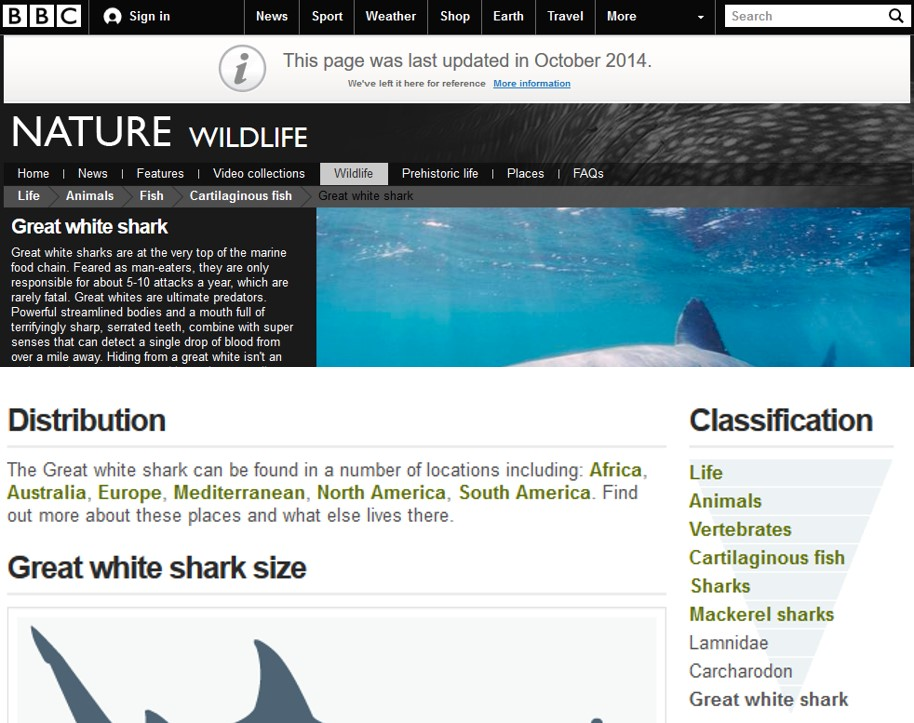
\includegraphics[width=5.0in]{media/ch5/figure-05-03.jpg}
    \caption{Great white shark at BBC: extract of the HTML rendering for
humans}
    \label{fig:ch5.3}
\end{figure}


When accessed by a Web browser for a human the response contains an HTML
page to be displayed (Figure~\ref{fig:ch5.3}) but when accessed by a machine the
response was a redirection to the RDF version of that description
(Figure~\ref{fig:ch5.4}) that could be found here:


\begin{lstlisting}
http://www.bbc.co.uk/nature/life/Great_white_shark.rdf
\end{lstlisting}

\begin{figure}
\begin{lstlisting}
<?xml version="1.0" encoding="utf-8"?><rdf:RDF
    xmlns:rdfs="http://www.w3.org/2000/01/rdf-schema#" 
    xmlns:rdf="http://www.w3.org/1999/02/22-rdf-syntax-ns#" 
    xmlns:owl="http://www.w3.org/2002/07/owl#" 
    xmlns:foaf="http://xmlns.com/foaf/0.1/" 
    xmlns:dc="http://purl.org/dc/terms/" 
    xmlns:dctypes="http://purl.org/dc/dcmitype/" 
    xmlns:skos="http://www.w3.org/2004/02/skos/core#"
    xmlns:xsd="http://www.w3.org/2001/XMLSchema#" 
    xmlns:po="http://purl.org/ontology/po/" 
    xmlns:wo="http://purl.org/ontology/wo/">
    		<rdf:Description rdf:about="/nature/species/Great_white_shark">
		<foaf:primaryTopic rdf:resource="/nature/species/Great_white_shark#species"/>
		<rdfs:seeAlso rdf:resource="/nature/species"/>
	</rdf:Description>
		<wo:Species rdf:about="/nature/life/Great_white_shark#species">
				<rdfs:label>Great white shark</rdfs:label>
				<wo:name rdf:resource="http://www.bbc.co.uk/nature/species/Great_white_shark#name"/>
	<foaf:depiction rdf:resource="http://ichef.bbci.co.uk/naturelibrary/images/ic/640x360/g/gr/great_white_shark/great_white_shark_1.jpg"/>
	<dc:description>Great white sharks are at the very top of the marine food chain. Feared as man-eaters, they are only responsible for about 5-10 attacks
\end{lstlisting}
    \caption{Great white shark at BBC: extract of the RDF/XML version for
machines}
    \label{fig:ch5.4}
\end{figure}

Moving to a completely different domain and data source, let us now
consider UniProt that provides RDF descriptions of protein sequence and
function. Again, if you are a biologist interested in the ``Cell surface
glycoprotein MUC18'', there is a URI for that:

\begin{lstlisting}
http://purl.uniprot.org/uniprot/P43121
\end{lstlisting}


\begin{figure}
    \centering
    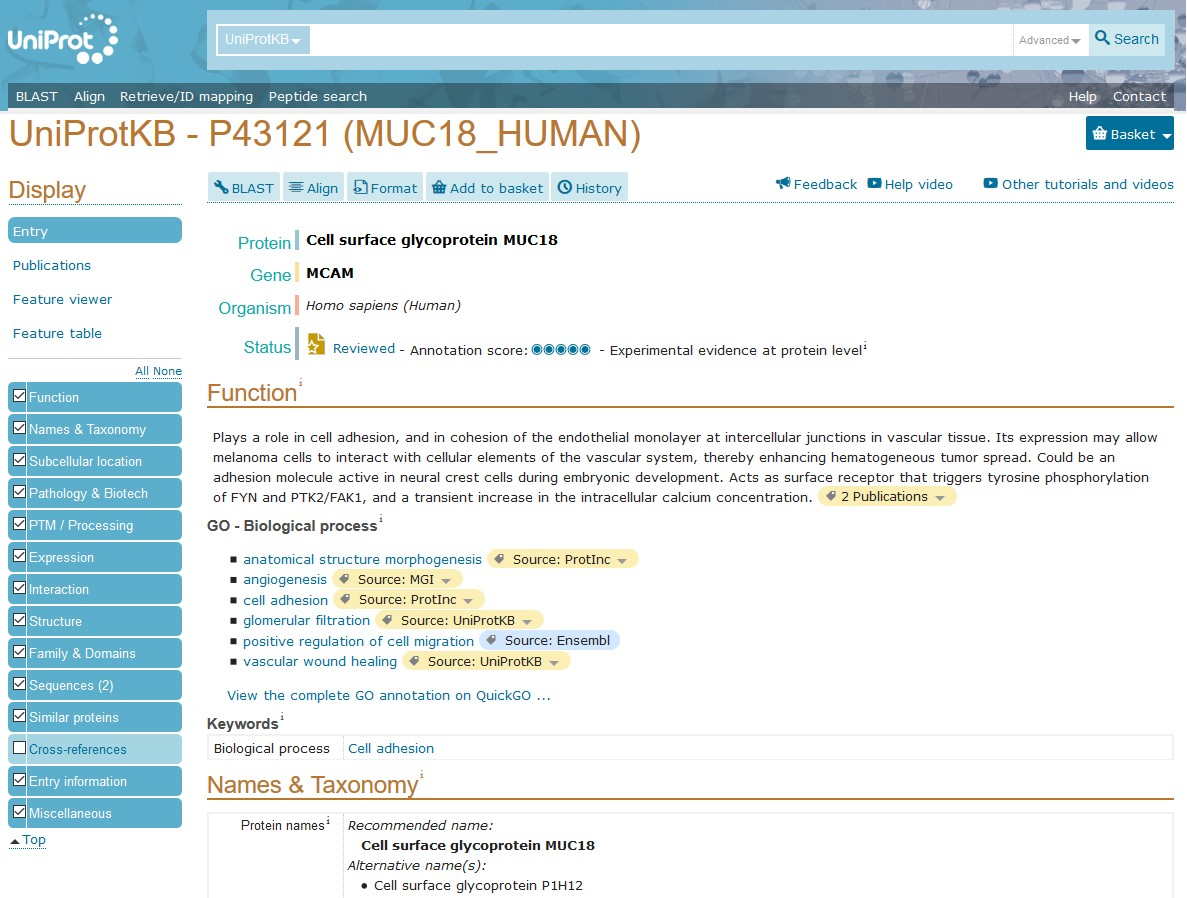
\includegraphics[width=5.0in]{media/ch5/figure-05-05.jpg}
    \caption{Cell surface glycoprotein MUC18 in UnitProt: extract of the HTML
rendering for humans}
    \label{fig:ch5.5}
\end{figure}

When accessed by a Web browser for a human the response contains an HTML
page to be displayed (Figure~\ref{fig:ch5.5}) but when accessed by a machine the
response is a redirection to the RDF version of that description (Figure~\ref{fig:ch5.6} that can be found here:

\begin{lstlisting}
https://www.uniprot.org/uniprot/P43121.rdf
\end{lstlisting}



\begin{figure}
\begin{lstlisting}
<rdf:RDF  (…)>
  <rdf:Description rdf:about="http://purl.uniprot.org/uniprot/P43121">
    <rdf:type rdf:resource="http://purl.uniprot.org/core/Protein"/>
    <reviewed rdf:datatype="http://www.w3.org/2001/XMLSchema#boolean">true</reviewed>
    <created rdf:datatype="http://www.w3.org/2001/XMLSchema#date">1995-11-01</created>
    <modified rdf:datatype="http://www.w3.org/2001/XMLSchema#date">2018-06-20</modified>
    <version rdf:datatype="http://www.w3.org/2001/XMLSchema#int">165</version>
    <mnemonic>MUC18_HUMAN</mnemonic>
    <oldMnemonic>MU18_HUMAN</oldMnemonic>
    <replaces rdf:resource="http://purl.uniprot.org/uniprot/O95812"/>
    <replaces rdf:resource="http://purl.uniprot.org/uniprot/Q59E86"/>
    <replaces rdf:resource="http://purl.uniprot.org/uniprot/Q6PHR3"/>
    <replaces rdf:resource="http://purl.uniprot.org/uniprot/Q6ZTR2"/>
    <citation rdf:resource="http://purl.uniprot.org/citations/2602381" rdf:ID="_P43121-citation-2602381"/>
    <citation rdf:resource="http://purl.uniprot.org/citations/8378324" rdf:ID="_P43121-citation-8378324"/>
    <citation rdf:resource="http://purl.uniprot.org/citations/11709656" rdf:ID="_P43121-citation-11709656"/>
\end{lstlisting}
    \caption{Cell surface glycoprotein MUC18 in UnitProt: extract of the
RDF/XML version for machines}
    \label{fig:ch5.6}
\end{figure}

As a third example let us consider DBpedia, which is according to their
own site, ``a crowd-sourced community effort to extract structured
content from the information created in various Wikimedia projects''
including the famous Wikipedia encyclopaedia. This initiatives extracts
and publicly makes available structured data from the pages of Wikipedia
and other Wikimedia projects, therefore covering a wide variety of
domains and topics. Again they use RDF and linked data principles
therefore every topic has a URI for which you can negotiate HRTML of
RDF. Consider for instance the topic ``Eiffel Tower'' identified by the
following identifier:

\begin{lstlisting}
{http://dbpedia.org/\textbf{resource}/Eiffel\_Tower
\end{lstlisting}

If you access that HTTP URI with a browser, you are redirected to the
following URL

\begin{lstlisting}
http://dbpedia.org/\textbf{page}/Eiffel\_Tower
\end{lstlisting}

This URL displays an HTML page rendering all the data extracted about
that topic and available publicly on the Web as linked data (Figure 7).

\begin{figure}
    \centering
    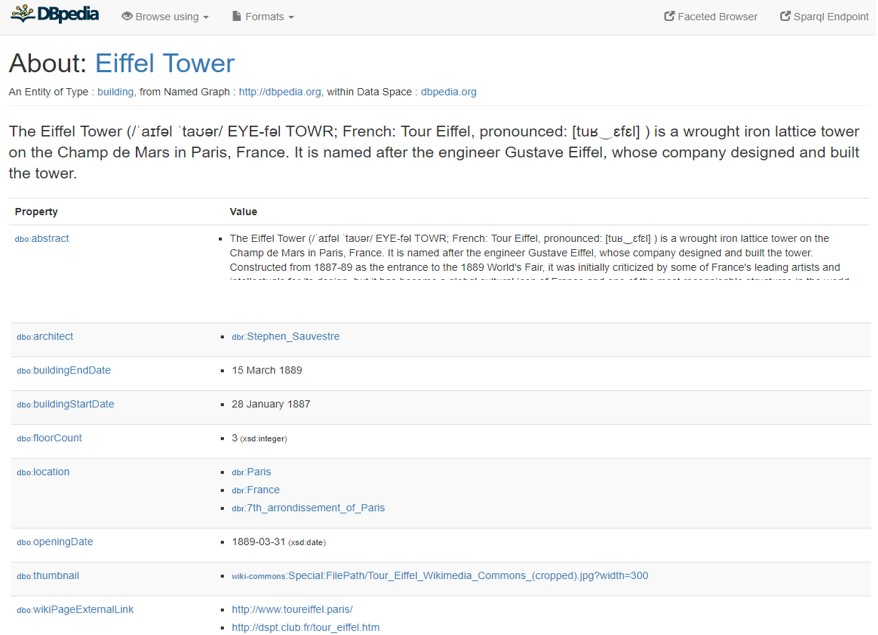
\includegraphics[width=5in]{media/ch5/figure-05-07.jpg}

    \caption{Eiffel Tower at DBpedia: extract of the HTML rendering for humans}
    \label{fig:ch5.7}
\end{figure}

At the same HTTP URI you can negotiate many other formats including, for
instance RDF using Turtle /N3 syntax. You would then be redirected
(Figure 8) to another URL for instance:

\url{http://dbpedia.org/data/Eiffel_Tower.n3}


\begin{figure}
 \begin{lstlisting}
1.	@prefix dbo:	<http://dbpedia.org/ontology/> .
2.	@prefix dbr:	<http://dbpedia.org/resource/> .
3.	@prefix rdf:	<http://www.w3.org/1999/02/22-rdf-syntax-ns#> .
4.	@prefix umbel-rc:	<http://umbel.org/umbel/rc/> .
5.	@prefix dbp:	<http://dbpedia.org/property/>
6.	@prefix wikidata:	<http://www.wikidata.org/entity/> .
7.	dbr:Eiffel_Tower
8.	rdf:type	umbel-rc:Skyscraper, wikidata:Q41176, umbel-rc:Building,
                    dbo:Location, dbo:Place, dbo:Building ;
9.	dbo:buildingStartDate	"28 January 1887" ;
10.	dbp:years	1889 ;
11.	dbo:floorCount	"3"^^xsd:positiveInteger ;
12.	dbp:mainContractor	dbr:Gustave_Eiffel ;
13.	dbo:location	dbr:Paris ,
14.	<http://dbpedia.org/resource/7th_arrondissement_of_Paris> ,
15.	dbr:France ;
16.	dbp:latd	48 ;
17.	dbp:latm	51 ;
18.	dbp:longd	2 ;
19.	dbp:longew	"E"^^rdf:langString ;
20.	dbp:longm	17 ;
21.	dbp:elevatorCount	8 ;
22.	dbp:height	300 .
 \end{lstlisting}
    \caption{Eiffel Tower at DBpedia: extract of the RDF/Turtle version for
machines}
    \label{fig:ch5.8}
\end{figure}

Now let us fully play the game of linked data. In (Figure 8) you can
find a piece of code (line 8) saying that the Eiffel Tower is of type
wikidata:Q41176 which is a qualified name using the prefix ``wikidata''
attached to a namespace (line 6). At this stage we don't know what this
means but we can follow our nose and expand the qualify name by
replacing the prefix with the namespace to obtain an HTTP URI that we
can access

\begin{lstlisting}
http://www.wikidata.org/\textbf{entity}/Q41176
\end{lstlisting}

If you access that HTTP URI with a browser, you are redirected to the
following URL

\begin{lstlisting}
https://www.wikidata.org/\textbf{wiki}/Q41176
\end{lstlisting}


This URL displays an HTML page rendering all the data about that
resource in another important data source of the Web of data: Wikidata
(Figure 9). This is another initiative of Wikimedia that provides as
central storage for the structured data used in other projects of the
foundation projects including Wikipedia, Wikivoyage, etc. This knowledge
base is open on the Web and can be read and edited by both humans and
machines.

\begin{figure}
    \centering
    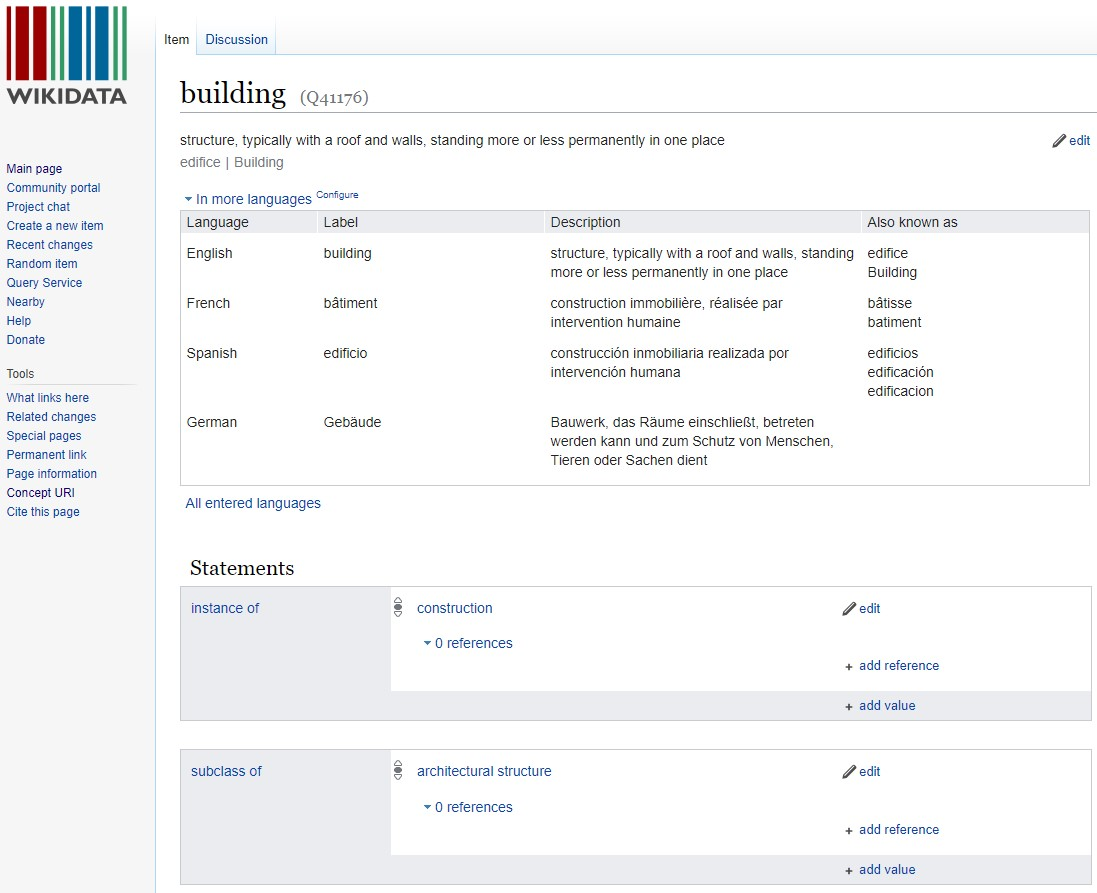
\includegraphics[width=5.0in]{media/ch5/figure-05-09.jpg}
    \caption{``Building'' at Wikidata: extract of the HTML rendering for humans}
    \label{fig:ch5.9}
\end{figure}

Again you can force the access to another format for the same data for
instance in RDF N-Triple (Figure 10). But if we now put all the pieces
together we can see that this mysterious resource called wikidata:Q41176
and found among the types of the Eiffel Tower in DBpedia represents the
category of the buildings in the data of Wikidata. So we see that these
linked data explain that the dataset of DBpedia the Eiffel Tower is
declared to be a Building in the sense of the dataset of Wikidata. We
witness a link across two data sources on the Web of data.

\begin{figure}
 \begin{lstlisting}
<http://www.wikidata.org/entity/Q41176> <http://www.w3.org/2000/01/rdf-schema#label> "building"@en .
<http://www.wikidata.org/entity/Q41176> <http://www.w3.org/2004/02/skos/core#prefLabel> "building"@en .
<http://www.wikidata.org/entity/Q41176> <http://schema.org/name> "building"@en .
<http://www.wikidata.org/entity/Q41176> <http://www.w3.org/2000/01/rdf-schema#label> "Bilding"@pih .
<http://www.wikidata.org/entity/Q41176> <http://www.w3.org/2004/02/skos/core#prefLabel> "Bilding"@pih .
<http://www.wikidata.org/entity/Q41176> <http://schema.org/name> "Bilding"@pih .
<http://www.wikidata.org/entity/Q41176> <http://www.w3.org/2000/01/rdf-schema#label> "budova"@sk .
<http://www.wikidata.org/entity/Q41176> <http://www.w3.org/2004/02/skos/core#prefLabel> "budova"@sk .
\end{lstlisting}
    \caption{Building at Wikidata: extract of the RDF N-Triple version for
machines}
    \label{fig:ch5.10}
\end{figure}

Until now we have used different tricks (different URLs) to see the
different formats available for each description avoiding to perform the
content negotiation ourselves. Let us now mention one way to perform
manually the dereferenciation of an HTTP URI and the content
negotiation. For this, you may use different tools or command and even
do it from a programming language if you want. Here we use the CURL
command line tool and library to transfer data using HTTP URIs. The
command may already be available on your machine or you may have to
install it from the Web site of the software\footnote{\url{https://curl.haxx.se/}}.
As show in Figure 11, this tool allow us to perform calls as command
lines and we performed two executions of CURL here on the same URL from
Wikidata we just saw. The first execution uses CURL with the options
``-o'' to save the output in a file named ``PageBuildings.html''. It
also uses the option ``-L'' to follow redirections and ``-H'' to specify
in the HTTP headers of our call that we want a response in HTML. The
last parameter is the URI of the category Buildings in Wikidata as seen
before. The result shows that CURL makes a first call, as a result it is
redirected to another address and makes a second call from which it
obtains and saves an HTML file of 230 kilobytes. The second execution is
almost the same except we specify in the HTTP headers of our call that
we want a response in RDF/XML and we save this second result in another
file named ``DataBuildings.rdf''. The result shows that again CURL makes
a first call, as a result it is redirected to another address and makes
a second call from which it obtains an RDF/XML file of 1620 kilo bytes

\begin{figure}
    \centering
    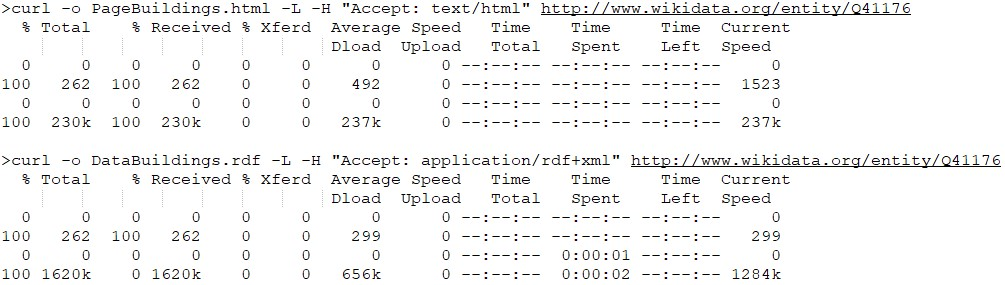
\includegraphics[width=5.0in]{media/ch5/figure-05-11.jpg}
    \caption{Performing CURL calls on Wikidata HTTP URIs to demonstrate
dereferencing and content negotiation}
    \label{fig:ch5.11}
\end{figure}

\hypertarget{linking-rdf-data}{%
\subsection{Linking RDF data}\label{linking-rdf-data}}

The recommended format to publish linked data on the Web is RDF and we
now know it has different serialization formats (XML, Turtle/N3,
JSON-LD, RDFa, etc.) that can be part of the content negotiation when
dereferencing an HTTP URI. The very fact RDF relies on URIs to identify
everything makes it an excellent data model to allow anyone to publish,
exchange and extend descriptions on the Web. The use of HTTP URIs
provide a standard way to obtain and augment data about any encountered
identifier. In fact, an RDF triple contains up to three HTTP URIs
(subject, predicate and object) and each can be used to ``follow our
noses'' and discover new data. Any HTTP URI used in an RDF description
can be looked-up for more information.

While it is true that any piece of RDF already contains links - since
RDF triples are links between a resource and (another) resource or a
literal -- this must be turned into a more specific best practice: to
weave a Web of linked data we need links across datasets which means the
subjects or objects of the triples of the dataset should reuse or link
URIs from other datasets as much as possible in order to generate that
global giant graph of data we want.

If each source was only using its own URIs within its own domain, then
each source would be an isolated island by default and there would be no
Web of data. As soon as external links are established either when the
data are created (e.g. reusing URIs) or after they were generated (e.g.
alignment) this supports the discovery, crawling, integration, browsing,
aggregation, etc. of multiple data sources in a Web of data.

The external links can be established in many different ways. First the
subject or object of the descriptions can reuse URIs from other
datasources. If the things described are already described somewhere
else in a different way, a new source may decide to reuse the URIs to
extend these descriptions; however the dereferenciation here would be
handled by the other site and this would lead to centralization of URIs.

More classically if the descriptions of a source (e.g. a catalog of
products) provide relations (e.g. ``Made In'') to other things (e.g.
geographical places) they may reuse URIs for descriptions about these
others things from other sources (e.g. a geographical linked dataset).
Related to the idea of alignment, the dataset can also provide
equivalence or identity links between URIs to assert for instance that
two different URIs are in fact identifying the same thing and provide
two different addresses to lookup for information about that same thing.

Finally every class or property used in an RDF description is also an
HTTP URI that, when looked up, can provide additional semantics and
support additional inferences. In addition, by reusing existing schemata
a description can be integrated to other datasets using the same
schemata and can be consumed by software that use same schemata. The
reuse of schemata fosters interoperability.

To find the schema of your dreams, like for anything on the Web, there
are Web applications providing directories and search engine
functionality. One of them is called LOV for Linked Open
Vocabularies\footnote{\url{http://lov.okfn.org/}} where you can find the
most well-known vocabularies and their links (Figure)

\begin{figure}
    \centering
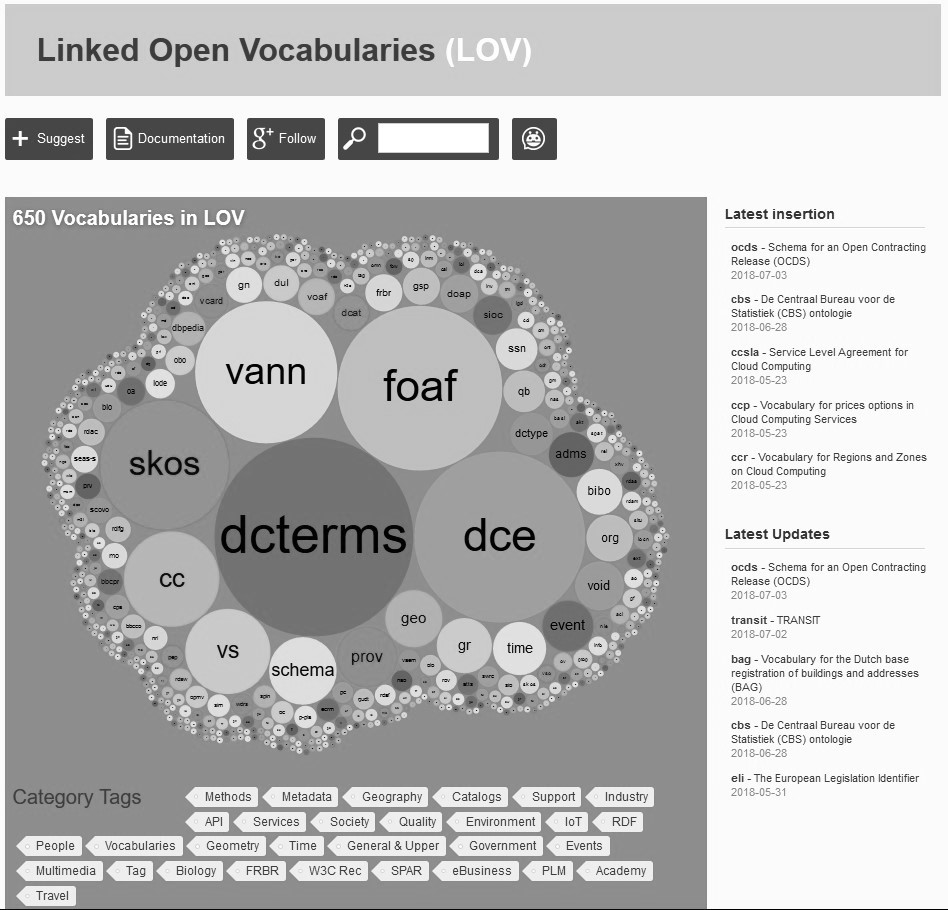
\includegraphics[width=5.0in]{media/ch5/figure-05-12.jpg}
    \caption{Linked Open Vocabularies (LOV) at OKFN}
    \label{fig:ch5.12}
\end{figure}

\hypertarget{cooking-a-web-of-linked-data-the-datatouille-metaphor}{%
\subsection{\texorpdfstring{Cooking a Web of linked data: the
\emph{Datatouille}
metaphor}{Cooking a Web of linked data: the Datatouille metaphor}}\label{cooking-a-web-of-linked-data-the-datatouille-metaphor}}

The overall process for producing and consuming linked data on the Web
may also be explained using a secret of ratatouille recipe. To obtain a
perfect ratatouille dish as cooked in the south of France one of the
tricks is to cook each vegetable separately (stage 1). Once each one is
properly cooked, the chef mixes them and cooks the ratatouille as one
dish (stage 2). Ratatouille is such a versatile dish, that it can be
used as an ingredient for other dishes such as (stage 3).

Preparing, publishing and (re)using linked data has a lot in common with
this process. Each data source is massaged and prepared separately by
its owner and with adequate applications. Each data provider has his own
constraints in terms of data selection (sensitivity, anonymity, etc.),
dataset features (velocity, volume, etc.) and data infrastructure
(legacy software, maintenance cost, etc.). Each source will therefore
cook its linked data separately (stage 1). Then anyone can use and link
to these published data and process them to produce new data: aggregated
data, statistics/mining/inference results, etc. (stage 2). In turn,
these new data become sources that their owners may publish as linked
data on the Web (stage 3).

\begin{figure}

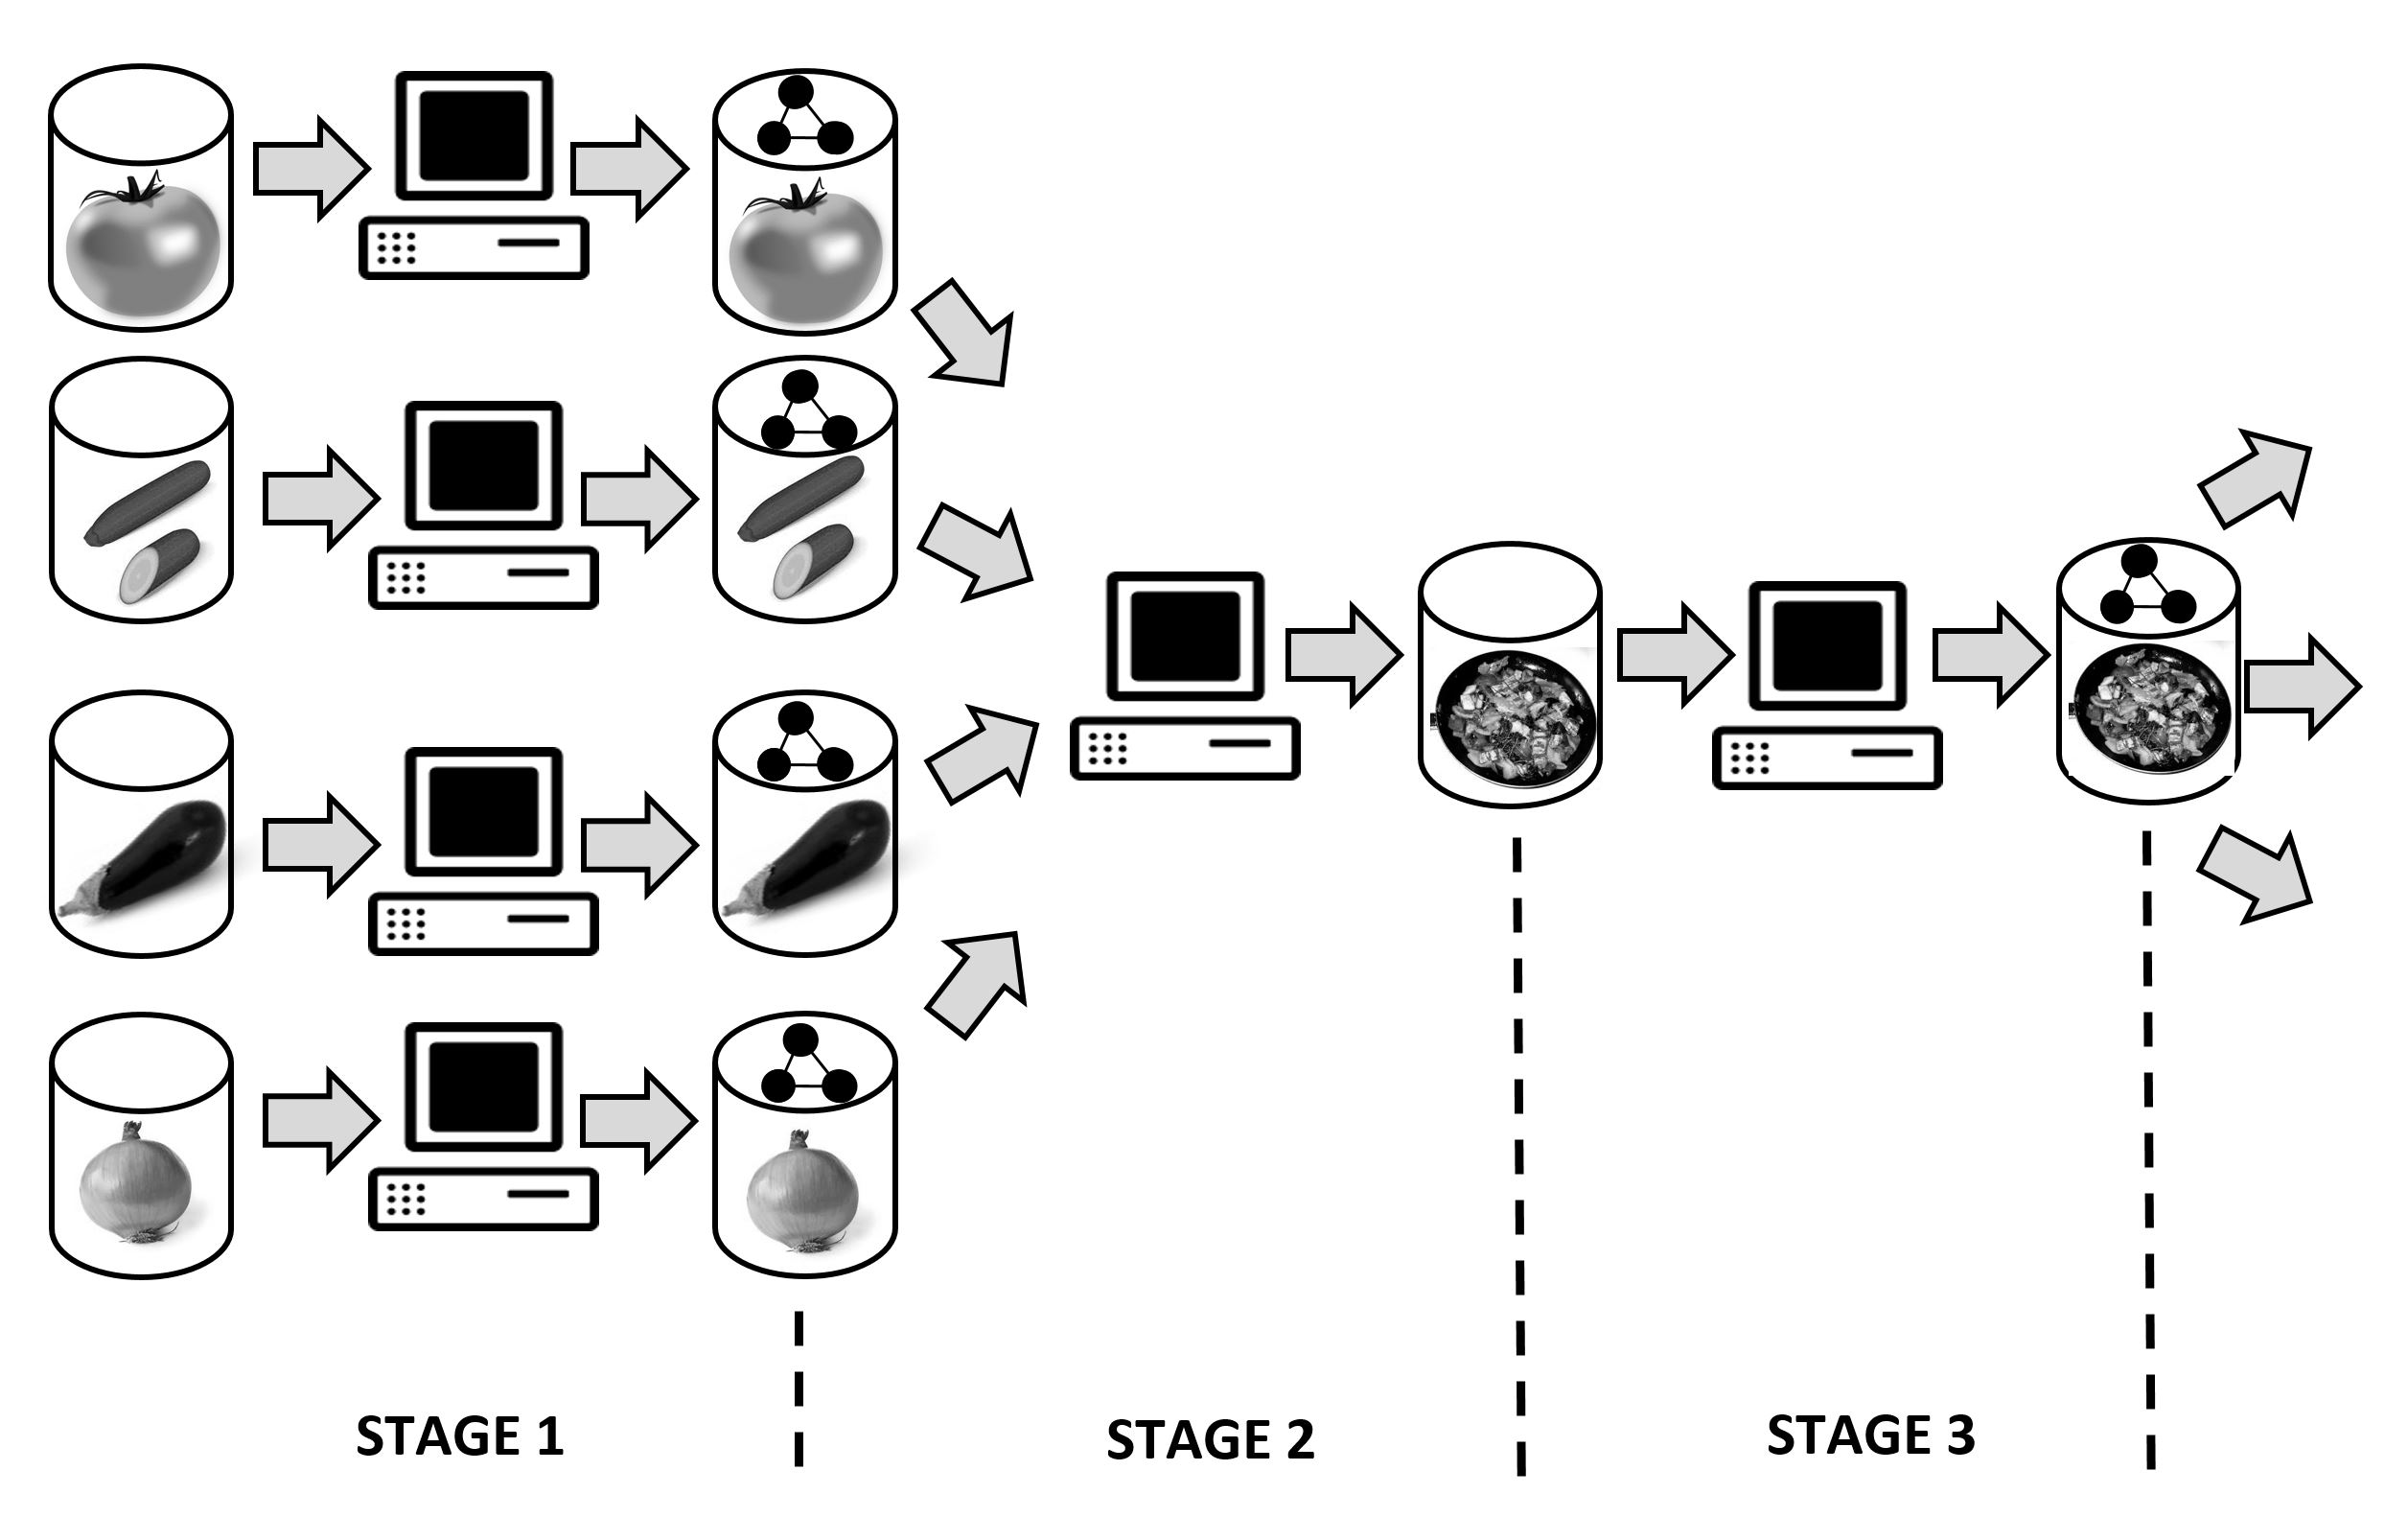
\includegraphics[width=5in]{media/ch5/figure-05-13x}
\label{fig:ch5.13x}
\caption{Three stages in producing linked data.}
\end{figure}

\hypertarget{linked-data-principles-in-a-mug}{%
\subsection{Linked data principles in a
mug}\label{linked-data-principles-in-a-mug}}

The W3C also found a way to summarize the linked data principles and had
it printed on mugs as what is called the 5-star deployment scheme for
Linked Data proposed by Tim Berners-Lee. The scheme is a cumulative list
of rules to lift Web data from one star to five stars. Each additional
rule to gain a star presumes the data meets the all of the previous
rules. The rules are given below and they cumulate to recommend that
data be available on the Web, in a non-proprietary structured format
using open W3C standards and linked to other data:

\begin{figure}
\begin{quote}
$\star{}$ Data is available on the Web, in whatever format.

$\star{}\star{}$ Available as machine-readable structured data, (i.e., not a scanned
image).

$\star\star\star$ Available in a non-proprietary format, (i.e, CSV, not Microsoft
Excel).

$\star\star\star\star$ Published using open standards from the W3C (RDF and SPARQL).

$\star\star\star\star\star$ All of the above and links to other Linked Open Data.
\end{quote}
\caption{Linked data principles from W3C}
\label{fig:ch5.13}
\end{figure}


\hypertarget{yet-another-cloud-for-the-web}{%
\subsection{Yet Another Cloud For the
Web}\label{yet-another-cloud-for-the-web}}

The term ``linked open data cloud'' or ``LOD Cloud'' does not refer to
the cloud paradigm of computer science but to of linked datasets
obtained by applying the linked data principles. This cloud is a graph
formed by nodes representing open datasets and edges indicating that the
data of two datasets are linked i.e. if one of the dataset reuses the
identifiers of the other dataset to identify the same resources (e.g.
persons, places, etc.). This cloud comprises only a small part the Web
of Data, made up of datasets that have declared at the Linked Open Data
Hub Web site, which collects and curates their descriptions before
compiling them into the Linking Open Data cloud diagram as shown in
figure 14.

\begin{figure}
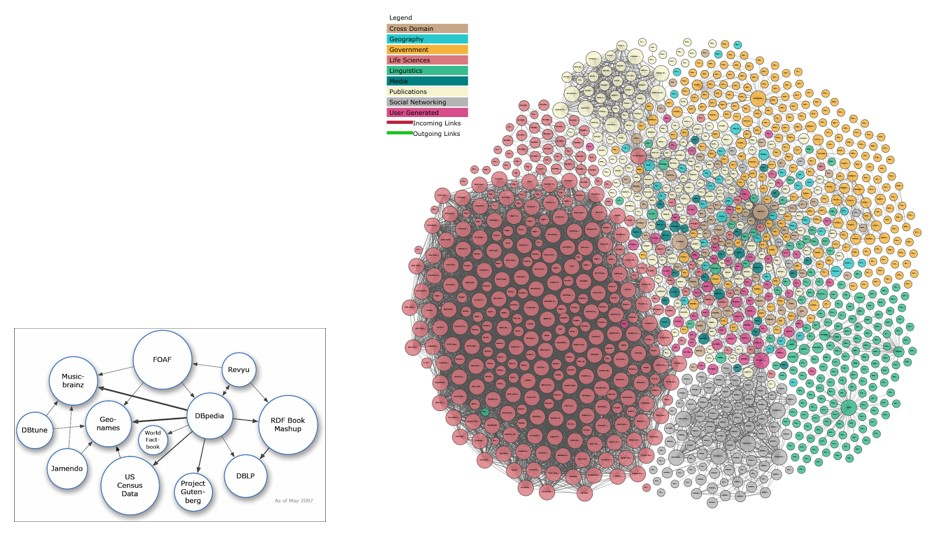
\includegraphics[width=5.0in]{media/ch5/figure-05-14.jpg}
\label{fig:ch5.14}
\caption{Linking Open Data cloud diagrams\protect\footnotemark\ ten years apart from 2007 (left) and 2017 (right)}
\end{figure}
\footnotetext{Andrejs Abele, John
  P. McCrae, Paul Buitelaar, Anja Jentzsch and Richard Cyganiak.
  http://lod-cloud.net/}

The 2017 edition of the diagram shown above shows a LOD cloud
aggregating 150 billion triples from nearly 3000 datasets. Every node
(circle) corresponds to a dataset, some of them very large in their own
right. The different colors show different domains of application (e.g.
life sciences, publication, governmental, geography).

Some of the sources included in this cloud are well-known for being
central, historic or atypical. Let us mention some of them:

\begin{itemize}
\item
  DBPedia is a central and historical source of data and identifiers in
  the linked open data cloud. It is one of the pioneering sources and
  its encyclopedic nature makes it well-suited as a source of reference
  for other datasets. Its name comes from the fact it publishes linked
  structured data extracted from Wikipedia and, in particular, from its
  \emph{infoboxes} (structured tables summarizing facts about a topic in
  a Wikipedia page). DBPedia includes all kinds of data, including birth
  dates of famous people, names of capital cities in different
  languages, geographical coordinates of landmarks, names and
  identifiers of drugs, etc. All of these data are available as linked
  open data.
\item
  Wikidata is an initiative of the Wikimedia foundation to crowdsource
  the contribution and maintenance of a central storage for the
  structured data to be used in other foundation projects including
  Wikipedia, Wikivoyage, etc. Here the approach is not to extract data
  from other sources but to directly edit and curate structured data in
  a Wiki manner. Then this structured data sources can be queried to
  generate content such a as tables or infoboxes in other sites. Again,
  all of these data are available as linked open data.
\item
  Geonames is a free geographical database that covers all countries
  and, at the time of this writing, contains over eleven million place
  descriptions (countries, cities, regions, etc.) with their names and
  information including currency, population, language, area,
  geographical coordinates, etc.
\item
  UniProt stands for Universal Protein Resource and is an international
  initiative to build and publish a comprehensive dataset of protein
  sequences and annotations.
\end{itemize}

In this book we included a number of examples from the Web such as the
data sources we just mentioned. At the time of writing these sources ae
available but anything can change on the Web at any moment and we
included several of them not only to show the variety but also to
account for the fact that some of them may change, move or even
disappear by the time you read these lines.

\hypertarget{validating-data}{%
\subsection{Validating data}\label{validating-data}}

Applications that publish and consume data from the Web of data are
written and hosted by very different organizations. Validation is a way
to ensure interoperability between open and heterogeneous as the ones
the Web architecture now links. Moreover, one of the strengths of RDF is
the simplicity and genericity of its standard graph data model but, as a
result, it is used to represent a huge variety of data and that variety
is one of the issues when processing big data. This means that the
quality of the data you will get may vary a lot from one source to
another. When discovering and exchanging data over the Web we therefore
need to check whether the data we obtain match what we expect in terms
of content and structure. This is also true when obtaining data from
users. In designing interactions with a user it is important to know
what information is mandatory and the constraints that must be met for
the input to be valid. If the user is entering their personal data, you
may want to check that the family name and first name have been provided
properly. If they are taking orders, you may want to ensure the product
ID and the quantity have been appropriately filled in, etc. All these
are examples of use cases for an RDF validation mechanism that allows us
to validate the data before adding them to our databases.

SHACL (Shapes Constraint Language) addresses the issue of data quality
at the structural level by providing a language to describe the
``shapes'' of the data you are expecting. This takes the form of an RDF
description of the constraints you want to enforce on the data,
including the required properties and the types of values you expect.
Once you have defined your constraints on the RDF data you are
interested in, you can check any piece of data from any source using a
validation software.

Imagine you design an application for collecting user profiles from the
Web. \emph{FOAF} (which stands for \emph{Friend of a Friend}) is a
popular vocabulary for representing user profile data on the Web of
data. Suppose that every time your application finds such a FOAF profile
on the Web, it wants to check its completeness with respect to some
requirements. As shown in Figure~\ref{fig:ch5.15}, the conditions are themselves
expressed in RDF and the core notion is the ``shape'' providing a
description that the data graphs need to satisfy. In our example, we
declare a shape (line 5) that targets resources of type foaf:Person
(line 7) and specified three constraints we would like to enforce. The
first constraint (lines 8-15) makes it compulsory to have exactly one
family name that must be a string of characters. The second constraint
(lines 16-24) makes it compulsory to have a gender and this must have
for value either ``male'' or ``female''. The third constraint (lines
25-28) just ensures that if the homepage is provided it is a valid IRI.

\begin{figure}
\begin{lstlisting}
1.	@prefix foaf: <http://xmlns.com/foaf/0.1/> .
2.	@prefix sh: <http://www.w3.org/ns/shacl#> .
3.	@prefix xsd: <http://www.w3.org/2001/XMLSchema#> .
4.	
5.	:PersonShape
6.	    a sh:NodeShape ;
7.	    sh:targetClass foaf:Person ;
8.	    sh:property [
9.	        sh:path foaf:familyName ;
10.	        sh:name "family name" ;
11.	        sh:description "the family name of a 
                                          person." ;
12.	        sh:datatype xsd:string ;
13.	        sh:maxCount 1 ;
14.	        sh:minCount 1 ;
15.	    ] ;
16.	    sh:property [
17.	        sh:path foaf:gender ;
18.	        sh:name "gender" ;
19.	        sh:description "the gender of a person 
                                 ('male' or 'female')." ;
20.	        sh:datatype xsd:string ;
21.	        sh:maxCount 1 ;
22.	        sh:minCount 1 ;
23.		sh:pattern "^(male|female)$" ;
24.	    ] ;
25.		sh:property [                
26.			sh:path foaf:homepage ;
27.			sh:nodeKind sh:IRI ;
28.		] .
\end{lstlisting}
\label{fig:5.15}
\caption{A SHACL shape to validate FOAF data: the shape is represented
itself in RDF.}
\end{figure}


If you provide such a SHACL shape to a SHACL validator, you can then
check if some data is valid with respect to these constraints. Consider
the data in Figure 16 containing two small FOAF profiles for Bob (lines
3-5) and Alice (lines 7-11). If you run a validator on these data the
report indicates that Alice is a valid foaf:Person according to your
constraints but that Bob is missing the gender property.

\begin{figure}
\begin{lstlisting}
1.	@prefix foaf: <http://xmlns.com/foaf/0.1/> .
2.	
3.	:Bob a foaf:Person ;
4.	    foaf:firstName "Robert" ;
5.	    foaf:familyName "Doe" .
6.	
7.	:Alice a foaf:Person ;
8.	    foaf:firstName "Alice" ;
9.	    foaf:familyName "Doe" ;
10.	    foaf:gender "female" ;
11.	    foaf:homepage <http://alice.homepage.com/> .
\end{lstlisting}
\label{fig:5.16}
\caption{Two FOAF profiles to be validated with the SHACL shape of Figure~\ref{fig:ch5.15}}
\end{figure}



SHACL provides a standard to specify structural patterns to be checked
upon the data by expressing rules about how actual RDF graphs or
subgraphs should look like in your data. This validation happens at the
structural level of the RDF graphs before considering any kind of
semantics or inference as we will see in the chapters about RDFS and
OWL. These structural constraints are already very useful to validate
and integrate data, to document data models, to generate user interfaces
or even code.

\hypertarget{the-linked-data-platform-architecture}{%
\subsection{The Linked Data Platform
architecture}\label{the-linked-data-platform-architecture}}

\emph{Representational State Transfer} (\emph{REST}) is a popular
software architecture style for creating and publishing services on the
Web. REST defines a set of constraints to ensure service
interoperability over the Web, based on accessing and manipulating
representations of resources through a uniform and predefined set of
operations (in particular, the standard HTTP methods \emph{GET},
\emph{PUT}, \emph{PATCH}, \emph{POST}, and \emph{DELETE}). A service
that complies with the REST principles is said to be \emph{RESTful}.

In a similar way, the W3C has defined the Linked Data Platform (LDP)
that specifies how web applications can publish, edit and delete
resources using the HTTP protocol. It can be seen as a standardized REST
access to linked data, describing how to build clients and servers that
create, read, and write linked data Resources.

Because in real applications you have to manage a variety of files and
data formats, LDP distinguishes two kinds of resources: resources with
an RDF representation (RDF descriptions) and resources using other
formats (e.g. HTML files, images, binary files).

In order to be able to add or remove resources from the Web, you need to
have some kind of data space in which to read and write these resources.
For this reason, LDP also introduces the notion of \emph{containers} to
group and manage resources. A container is collections of resources,
often homogeneous ones (e.g. a collection of user profiles, a catalog of
book descriptions, an inventory of cars). LDP supports three kinds of
containers with more or less support to automate the creation of
membership relations between the resources and their containers. A
\emph{Basic Container} provides a simple containment vocabulary and
access mechanism. A \emph{Direct Container} supports the use of a
domain-specific membership assertions (e.g. assert a relation called
``author'' between all the resources of a collection of books and a
resource representing their author). An \emph{Indirect Container} allows
you to control more precisely the URI of the domain-specific member
resources you create.

LDP specifies the effect that each HTTP verb has on resources and
containers. Figure 17 summarizes each case and shows how these standard
methods allow you to use only HTTP to remotely manage resources and
containers in any LDP-compliant platform.


\begin{figure}
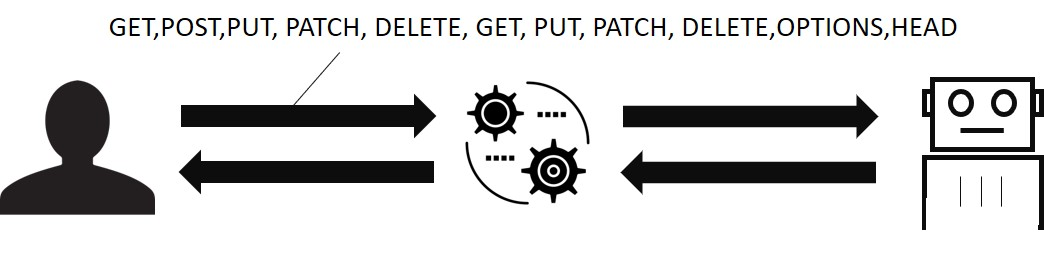
\includegraphics[width=5.0in]{media/ch5/figure-05-17.jpg}
\begin{tabular}{|lll|}
\hline
\textbf{Resource type} & \textbf{Method} & \textbf{Result}\tabularnewline
\hline\hline
Container & GET & Lists all the members of the container\tabularnewline
& POST & Create a new member of the container\tabularnewline
& PUT & Update the description of the container\tabularnewline
& PATCH & Partial update of the description of the
container\tabularnewline
& DELETE & Delete the container\tabularnewline
\hline
Any other resource type & GET & Retrieve a representation of the
resource\tabularnewline
& PUT & Update the resource description\tabularnewline
& PATCH & Partial update of the resource description\tabularnewline
& DELETE & Delete the resource description\tabularnewline
\hline\hline
Container or resource & OPTIONS & Discover the allowed operations over a
resource\tabularnewline
& HEAD & Only retrieve meta-information about a resource\tabularnewline
\hline
\end{tabular}
 \label{fig:ch5.17}
 \caption{The effects of HTTP verbs as specified in LDP}
\end{figure}


Figure~\ref{fig:ch5.18} shows the transcript of an HTTP request (lines 1-13) sent to a
container (/fabien/, line 1) on an LDP platform on a Web server
(inria.fr). The request uses the verb POST (line 1). As we saw in Figure
17, POST to a container creates a new member of that container. The
request provides the description of the RDF resource in Turtle
(serialization specified in line 4) and directly includes the data for
the new resource in the request itself (lines 7-13). The result (lines
15-18) shows that the request was accepted by the server (line 16), the
resource was created (also line 16), and it provides the URI of the
newly created description is returned (line 17).

\begin{figure}
  
    \label{fig:ch5.18}
\begin{lstlisting}
1.	POST /fabien/ HTTP/1.1
2.	Host: inria.fr
3.	Link: <http://www.w3.org/ns/ldp#Resource>; rel="type"
4.	Content-Type: text/turtle
5.	Slug: foaf
6.	
7.	@prefix foaf: <http://xmlns.com/foaf/0.1/> .
8.	@prefix dc: <http://purl.org/dc/terms/> .
9.	<> a foaf:PersonalProfileDocument;
10.	   foaf:primaryTopic <#me> ;
11.	   dc:title 'Fabien’s FOAF profile' .
12.	<#me> a foaf:Person;
13.	   foaf:name 'Fabien Gandon' .
14.	 
15.	 
16.	HTTP/1.1 201 Created
17.	Location: http://inria.fr/fabien/foaf
18.	Link: <http://www.w3.org/ns/ldp#Resource>; rel="type"
19.	Content-Length: 0

\end{lstlisting}
  \caption{Example of a POST request on an LDP container and its result}
  \end{figure}

\hypertarget{summary}{%
\subsection{Summary}\label{summary}}

To weave a Web of linked data you must follow three rules: (1) use HTTP
URIs to name everything (2) provide descriptive information in
appropriate formats about the resources identified by these URIs every
time they are accessed, and (3) include, in these descriptions, links to
HTTP URIs of other things. We have seen how to mint the URIs and how
HTTP can be used to negotiate the best answer when dereferencing a URI.
Web agents may need to validate data that comes from the Web or its
users. For this purpose, the Semantic Web stack provides SHACL, a
language for specifying ``shapes'' for data, which specify structural
constraints to be met by a piece of RDF to be valid. Finally, we saw how
the Linked Data Platform (LDP) provides a standardized service
architecture and set of operations based on HTTP verbs to read and write
resources and resource descriptions on the Web of data.

\hypertarget{fundamental-concepts}{%
\subsection{Fundamental concepts}\label{fundamental-concepts}}

The following fundamental concepts were introduced in this chapter:

\begin{itemize}
\item
  HTTP URIs and dereferencing: a URIs created to name anything but that
  uses the HTTP in order to be dereferenceable by just making and HTTP
  call to the address it provides.
\item
  the content negotiation in HTTP allowing a server to serve for the
  same HTTP URI different contents to Web clients.
\item
  SHACL shapes to validate RDF data at the structural level by providing
  the constraint you expect them to meet.
\item
  Linked Data Platform (LDP) that specifies how web applications can
  publish, edit and delete resources using the HTTP protocol.
\end{itemize}


\chapter{Querying the Semantic Web -- SPARQL}
\label{ch6}

RDF provides a simple way to represent distributed data. The triple is
the simplest way to represent a named connection between two things. But
a representation of data is useless without some means of accessing that
data. The standard way to access RDF data uses a query language called
SPARQL. SPARQL stands for SPARQL Protocol And RDF Query Language (yes,
the ``S'' in ``SPARQL'' stands for ``SPARQL,'' sigh). The SPARQL query
language works closely with the structure of RDF itself. SPARQL query
patterns are represented in a variant of Turtle (the same language that
we use to express RDF throughout this book). The queried RDF graph can be created from one
kind of data or merged from many; in either case, SPARQL is the way to
query it.

This chapter gives examples of the SPARQL query language. Most of the
examples are based on version 1.0 of the standard, released in 2008. More advanced features 
are now available in the more recent SPARQL 1.1 release.  SPARQL 1.1 is backward compatible with
SPARQL 1.0, so the basic features are available for both releases. 

SPARQL is a query language and shares many features with other query
languages like XQUERY and SQL. But it differs from each of these query
languages in important ways (as they differ from one another). Since we
don't want to assume that a reader has a background in any specific
query language (or even query languages at all), we begin with a gentle
introduction to querying data. We start with the most basic information
retrieval system, which we call a Tell-and- Ask system.

\section{Tell-And-Ask Systems}

A Tell-and-Ask system is a simple system -- you tell it some facts, and
then it can answer questions you ask based on what you told it. Consider the following simple example:

\textbf{Tell:} James Dean played in the movie \emph{Giant}. Then you could ask
questions like:

\textbf{Ask:} Who played in \emph{Giant}?

\textbf{Answer:} James Dean

\textbf{Ask:} James Dean played in what?

\textbf{Answer:} ``\emph{Giant}

You might tell it some more things, too, like:

\textbf{Tell:} James Dean played in \emph{East of Eden}. 
\textbf{Tell:} James Dean played in \emph{Rebel without a Cause}.

Then if you ask:

\textbf{Ask:} James Dean played in what?

\textbf{Answer:} \emph{Giant}, \emph{East of Eden}, \emph{Rebel without a Cause}.

One could imagine a sophisticated Tell-and-Ask system that understands
natural language and can cope with questions like

\textbf{Ask:} What movies did James Dean star in?

\textbf{Answer:} \emph{Giant}, \emph{East of Eden}, \emph{Rebel without a Cause}.

Instead of using the simplified language in these examples. As we shall
see, most real Tell-and-Ask systems don't do anything with natural
language processing at all. In more complex Tell-and-Ask 
systems, it can be quite difficult to be very specific about just what
you really want to ask, so they usually use languages that are quite
precise and technical.

On the face of it, it might seem that Tell-and-Ask systems aren't very
interesting. They don't figure out anything you didn't tell them
yourself. They don't do any calculations, they don't do any analysis.
But this judgment is premature; even very simple Tell-and-Ask systems
are quite useful. Let's have a look at one -- a simple address book.

You have probably used an address book at some point in your life. Even
a paper-and-pencil 
address book is a Tell-and-Ask system, though the process of telling it
something (i.e., writing down an address) and the process of asking it
something (looking up an address) take a lot of human effort. Let's
think instead of a computer program that does the job of an address
book. How does it work?

Like a paper address book, you tell it names and addresses (and probably
phone numbers and email addresses and other information). Unlike the
sample Tell-and-Ask system that we used to talk about James Dean and
movies, you probably don't talk to your address book in anything that
remotely resembles English; you probably fill out a form, with a field
for a name, and another for the parts of the address, and so on. You
``tell'' it an address by filling in a form.

How do you ask a question? If you want to know the address of someone,
you type in their name, perhaps into another form, very similar to the
one you filled in to tell it the information in the first place. Once
you have entered the name, you get the address.

The address book only gives you back what you told it. It does no
calculations and draws no conclusions. How could this be an interesting
system? Even without any ability to do computations, address books are
useful systems. They help us organize certain kinds of information that
is useful to us and to find it when we need it. It is a simple
Tell-and-Ask system -- you tell it things, then you ask questions.

Even the address book is a bit more advanced than the simplest
Tell-and-Ask system. When you look up an address in an address book, you
usually get a lot more information than just the address. It is as if
you asked a whole set of questions:

\textbf{Ask:} What is the address of Maggie Smith?

\textbf{Ask:} What is the phone number of Maggie Smith? 

\textbf{Ask:} What is the email address of Maggie Smith? And so on.

How can we make our address book system a bit more useful? There are a
number of ways to enhance its behavior (and many of these are available
in real address book applications). One way to make the address book
``smarter'' is to require less of the user who is asking questions. For
instance, instead of typing in ``Maggie Smith'' when looking for an
address, the system could let you just type in ``Maggie,'' and look for
any address where the name of the addressee contains the word
``Maggie.'' Now it is as if you have asked

\textbf{Ask:} What is the address of everyone whose name includes ``Maggie''?

You might get more answers if you do this -- if, for instance, you also
have an address for Maggie
King, you'll get both addresses in response to your question.

You can go even further -- you can ask your question based on some other
information. You could ask about the address instead of the name, by
filling in information in the address field:

\textbf{Ask:} Who lives at an address that contains ``Downing''?

\subsection{Common tell-and-ask infrastructure -- spreadsheets}

The address book was an example of a special-purpose tell-and-ask
system; it is aimed at a single task and has a fixed structure to the
information you can tell it and ask it about. A spreadsheet is an
example of a tell-and-ask system that is highly configurable and can be
applied to a large number of situations. Spreadsheets are often cited as
the most successful ``killer application'' ever; putting data management
into the hands of intelligent people without the need to learn any
heavy-duty technical skills. Spreadsheets apply the notion of WYSIWYG
(What You See Is What You Get) to data management; a visual
representation of data.

The ``language'' for telling information to a spreadsheet and asking
information of a spreadsheet is visual; information is entered into a
particular row and column and is retrieved by visually inspecting the
table.

Since spreadsheets are primarily a visual presentation of data, you
don't communicate with them in any particular language -- much less
natural language. You don't write ``where does Maggie live?'' to a
spreadsheet; instead you search for Maggie in the ``Name'' column and
look into the ``address'' column to answer your question.

Spreadsheets become more cumbersome when the data aren't conveniently
represented in a single table. Probably the simplest example of data
that don't fit into a table is multiple values. Suppose we have more
than one email address for Maggie Smith. How do we deal with this? We
could have multiple email columns, like this:

\begin{tabular}{|l l l|}
\hline
Name&Email1&Email2\\
\hline
Maggie Smith&MSmith@acme.com&maggie@gmail.com \\
\hline
\end{tabular}

This solution works as long as nobody has three email addresses, etc.
Another solution is to have a new row for Maggie, for each email address

\begin{tabular}{|l l|}
\hline
Name&Email \\
\hline
Maggie Smith&MSmith@acme.com\\
Maggie Smith&maggie@gmail.com\\
\hline
\end{tabular}

This is a bit confusing, in that it is unclear whether we have one
contact named ``Maggie Smith'' with two emails, or two contacts who
happen to have the same name, one with each email address.

Spreadsheets also start to break down when an application requires
highly interconnected data. Consider a contacts list that maintains
names of people and the companies they work for. Then they maintain
separate information for the companies -- billing information, contract
officer, etc. If this information is put into a single table, the
relationship between the company and its information will be duplicated
for each contact that works at that company, as illustrated in the table
below:

\begin{tabular}{|l l l l l|}
\hline
Name&Email&Company&Contract Officer&Headquarters\\
\hline
Maggie Smith&MSmith@acme.com&ACME Product Inc.&Cynthia Wiley&Pittsburgh\\
Maggie Smith&MKing@acme.com&ACME Product Inc.&Cynthia Wiley&Pittsburgh\\
\hline
\end{tabular}

Both Maggies work for ACME, where the Contract Officer is Cynthia and
the headquarters is in Pittsburgh. Duplicating information in this
manner is error-prone as well as wasteful; for instance, if ACME gets a
new contract officer, all the contact records for people who work for
ACME need to be changed.

A common solution to this problem is to separate out the company
information from the contact information into two tables, e.g.:

\begin{tabular}{|lll|}
\hline
Name&Email&Company\\
\hline
Maggie Smith&MSmith@acme.com&ACME Product Inc. \\
Maggie Smith&MKing@acme.com&ACME Product Inc. \\
\hline
\end{tabular}

\phantom{I}

\begin{tabular}{|lll|}
\hline
Company&Contract Officer&Headquarters\\
\hline
Acme Product Inc.&Cynthia Wiley&Pittsburgh\\
\hline
\end{tabular}



This sort of solution is workable in modern spreadsheet software but
begins to degrade the main advantages of spreadsheets; we can no longer
use visualization to answer questions. Its structure relies on
cross-references that are not readily visible by examining the
spreadsheet. In fact, this sort of solution moves the tell-and-ask
system from spreadsheets into a more structured form of tell-and-ask
system, a relational database.

\subsection{Advanced tell-and-ask infrastructure -- relational database}

Relational databases form the basis for most large-scale tell-and-ask
systems. They share with spreadsheets a tabular presentation of data but
include a strong formal system (based on a mathematical formalism called
the ``relational algebra'') that provides a systematic way to link
tables together. This facility, along with some well-defined
methodological support, allows relational data- bases to represent
highly structured data, and respond to very detailed, structured
questions.

\textbf{Tell:} Maggie King works for Acme Product Inc.

\textbf{Tell:} The contract officer for Acme Product Inc. is Cynthia Wiley

\textbf{Tell:} Cynthia Wiley's email address is
\href{mailto:CJWiley@acme.com}{CJW}\href{mailto:iley@acme.com}{\nolinkurl{iley@acme.com}}

\textbf{Ask:} What is the email address for the contract officer at the company
where Maggie King works?

\textbf{Answer:}
\href{mailto:CJWiley@acme.com}{CJW}\href{mailto:iley@acme.com}{\nolinkurl{iley@acme.com}}

This sort of detailed structure comes at a price -- asking a question
becomes a very detailed process, requiring a specialized language. Such
a language is called a query language.

In the query language for relational databases, links from one table to
another are done by cross-referencing.  A closer rendering of the
question above, in a query language for a relational database, would be:

\textbf{Ask:} What is the email address for the person matched by the ``contract
officer'' reference for the company matched by the ``works for''
reference for the person whose name is ``Maggie King''? Answer:
\href{mailto:CJWiley@acme.com}{CJW}\href{mailto:iley@acme.com}{\nolinkurl{iley@acme.com}}

This might seem like a needlessly wordy way to ask the question, but
this is how you pose questions precisely enough to recover information
from a complex database structure.

\section{RDF as a Tell-And-Ask System}

RDF is also a tell-and-ask system. Like a relational database, RDF can
represent complex structured data. Also like a relational database, RDF
requires a precise query language to specify questions. Unlike a
relational database, the cross-references are not visible to the end
user, and there is no need to explicitly represent them in the query
language.

As discussed in previous chapters, in RDF, relationships are represented
as triples. Asserting a triple amounts to TELLing the triple store a
fact.

\textbf{Tell:} James Dean played in the movie \emph{Giant}.

How do we ASK questions of this? Even with a single triple, there are
already some questions we could ask:

\textbf{Ask:} What did James Dean play in?

\textbf{Ask:} Who played in \emph{Giant}?

\textbf{Ask:} What did James Dean do in \emph{Giant}?

All of these questions can be asked in SPARQL in a simple way, by
replacing part of the triple with a question word, like Who, What,
Where, etc. SPARQL doesn't actually distinguish between question words,
so we can choose words that make sense in English. In SPARQL, question
words are written with a question mark at the start, e.g., \texttt{?who}, \texttt{?where},
\texttt{?when}, etc.

\textbf{Ask:} James Dean played in ?what

\textbf{Answer:} \emph{Giant}

\textbf{Ask:} ?who played in \emph{Giant}

\textbf{Answer:} James Dean

\textbf{Ask:} James Dean ?what \emph{Giant}

\textbf{Answer:} played in

This is the basic idea behind SPARQL -- that you can write a question
that looks a lot like the data, with a question word standing in for the
thing you want to know. Like query languages for relational databases
and spreadsheets, SPARQL makes no attempt to mimic the syntax of natural
language, but it does use the idea that a question can look just like a
statement, but with a question word to indicate what we want to know.

\section{SPARQL -- QUERY LANGUAGE FOR RDF}

The syntax of SPARQL actually looks like Turtle. So these examples
really look more like this:

\textbf{\textbf{Tell:}} :JamesDean :playedIn :Giant . 

\textbf{\textbf{Ask:}} :JamesDean :playedIn ?what .

\textbf{\textbf{Answer:}} :Giant

\textbf{\textbf{Ask:}} ?who :playedIn :Giant .

\textbf{\textbf{Answer:}} :JamesDean

\textbf{\textbf{Ask:}} :JamesDean ?what :Giant .

\textbf{\textbf{Answer:}} :playedIn

Before we go further, let's talk a bit about the syntax of a SPARQL
query. We'll start with a simple form, the SELECT query. Readers
familiar with SQL will notice a lot of overlap with SPARQL syntax (e.g.,
keywords like SELECT and WHERE). This is not coincidental; SPARQL was
designed to be easily learned by SQL users.

A SPARQL SELECT query has two parts; a set of question words, and a
question pattern. The keyword WHERE indicates the selection pattern,
written in braces. We have already seen some question patterns, e.g.,

\begin{lstlisting}
WHERE :JamesDean :playedIn ?what .
WHERE ?who :playedIn :Giant .
WHERE :JamesDean ?what :Giant .
\end{lstlisting}

The query begins with the word SELECT followed by a list of the question
words. So the queries for the questions above are

\begin{lstlisting}
SELECT ?what WHERE :JamesDean ?playedIn ?what .
SELECT ?who WHERE ?who :playedIn :Giant .
SELECT ?what WHERE :JamesDean ?what :Giant .
\end{lstlisting}

It might seem that listing the question words in the SELECT part is
redundant -- after all, they appear in the patterns already. Not all the
question words need to be in the SELECT and only those mentioned in the
SELECT will actually be given in the results. and we'll see later how
modifying this list can be useful.

RDF (and SPARQL) deals well with multiple values. If we TELL the system
that James Dean played
in multiple movies, we can do this without having to make any
considerations in the representation:

\textbf{Tell:}
\begin{lstlisting}
   :JamesDean :playedIn :Giant .
   :JamesDean :playedIn :EastOfEden .
   :JamesDean :playedIn :RebelWithoutaCause .
\end{lstlisting}

Now if we ASK a question with SPARQL

\textbf{\textbf{Ask:}} 
\begin{lstlisting}
SELECT ?what WHERE {:JamesDean :playedIn ?what}
\end{lstlisting}
\textbf{\textbf{Answer:}} :Giant, :EastOfEden, :RebelWithoutaCause.

The WHERE clause of a SPARQL query can be seen as a graph pattern, that
is, a pattern that is matched against the data graph. In this case, the
pattern has just one triple, \texttt{:JamesDean} as the subject, \texttt{:playedIn} as the
predicate, and a question word as the object. The action of the query
engine is to find all matches for the pattern in the data, and to return
all the values that the question word matched.

We can see this as a graph -- Figure~\ref{fig:ch06.1} shows the James Dean data in
the form of a graph, and the WHERE clause as a graph pattern. There are
three matches for this pattern in the graph, where a match has to match
resources in the pattern exactly, but anything can match the question
word.

Suppose we follow the data along further. Each of these movies is
directed by someone. Some of them might be directed by more than one
person, as shown in Figure 5.2. Who were the directors that

\begin{figure}
\centering
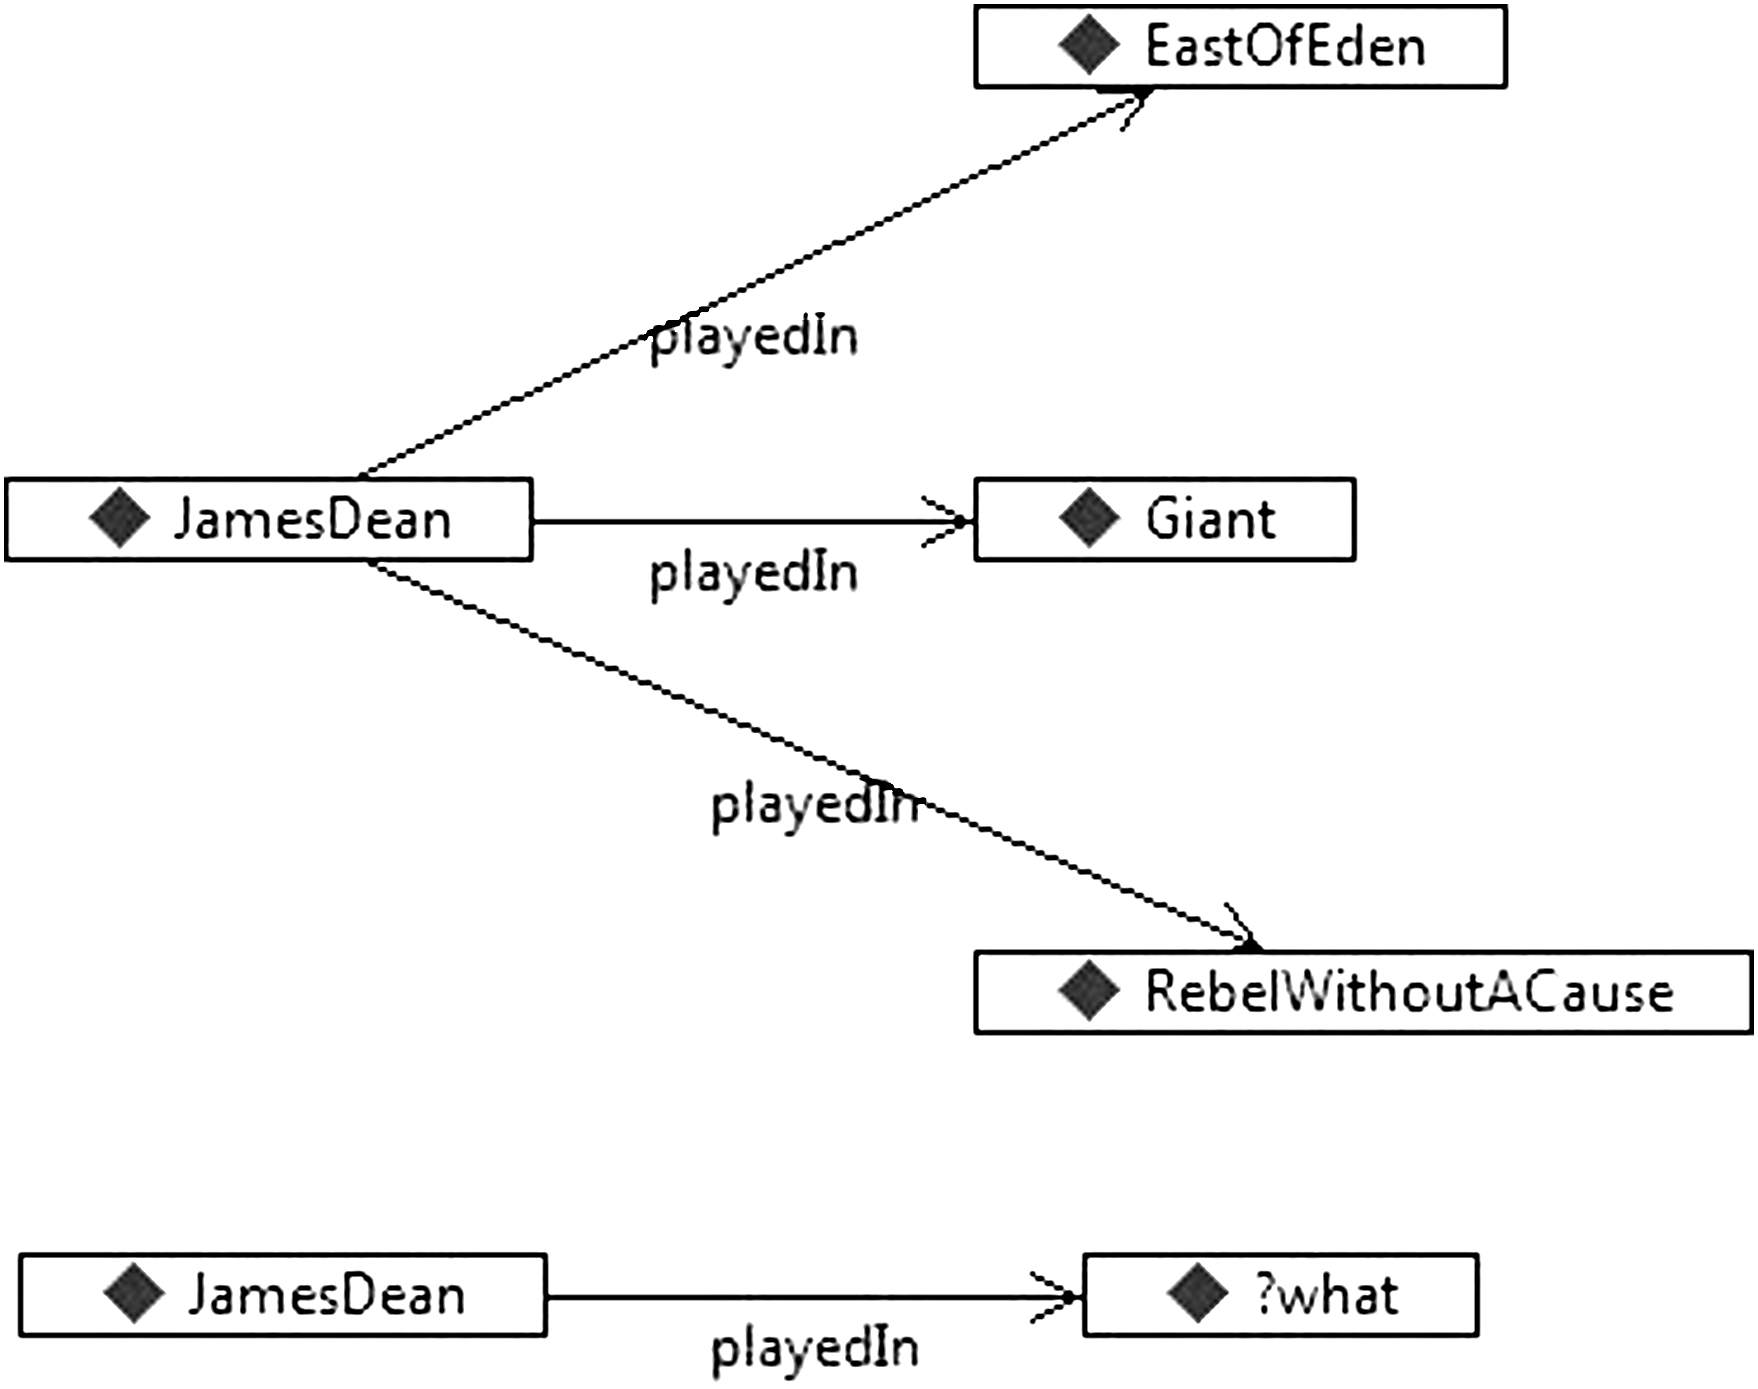
\includegraphics[width=5in]{media/f06-01.png}
\label{fig:ch06.1}
\caption{James Dean data in a graph, and a query to fetch it.}
\end{figure}

\begin{figure}
\centering
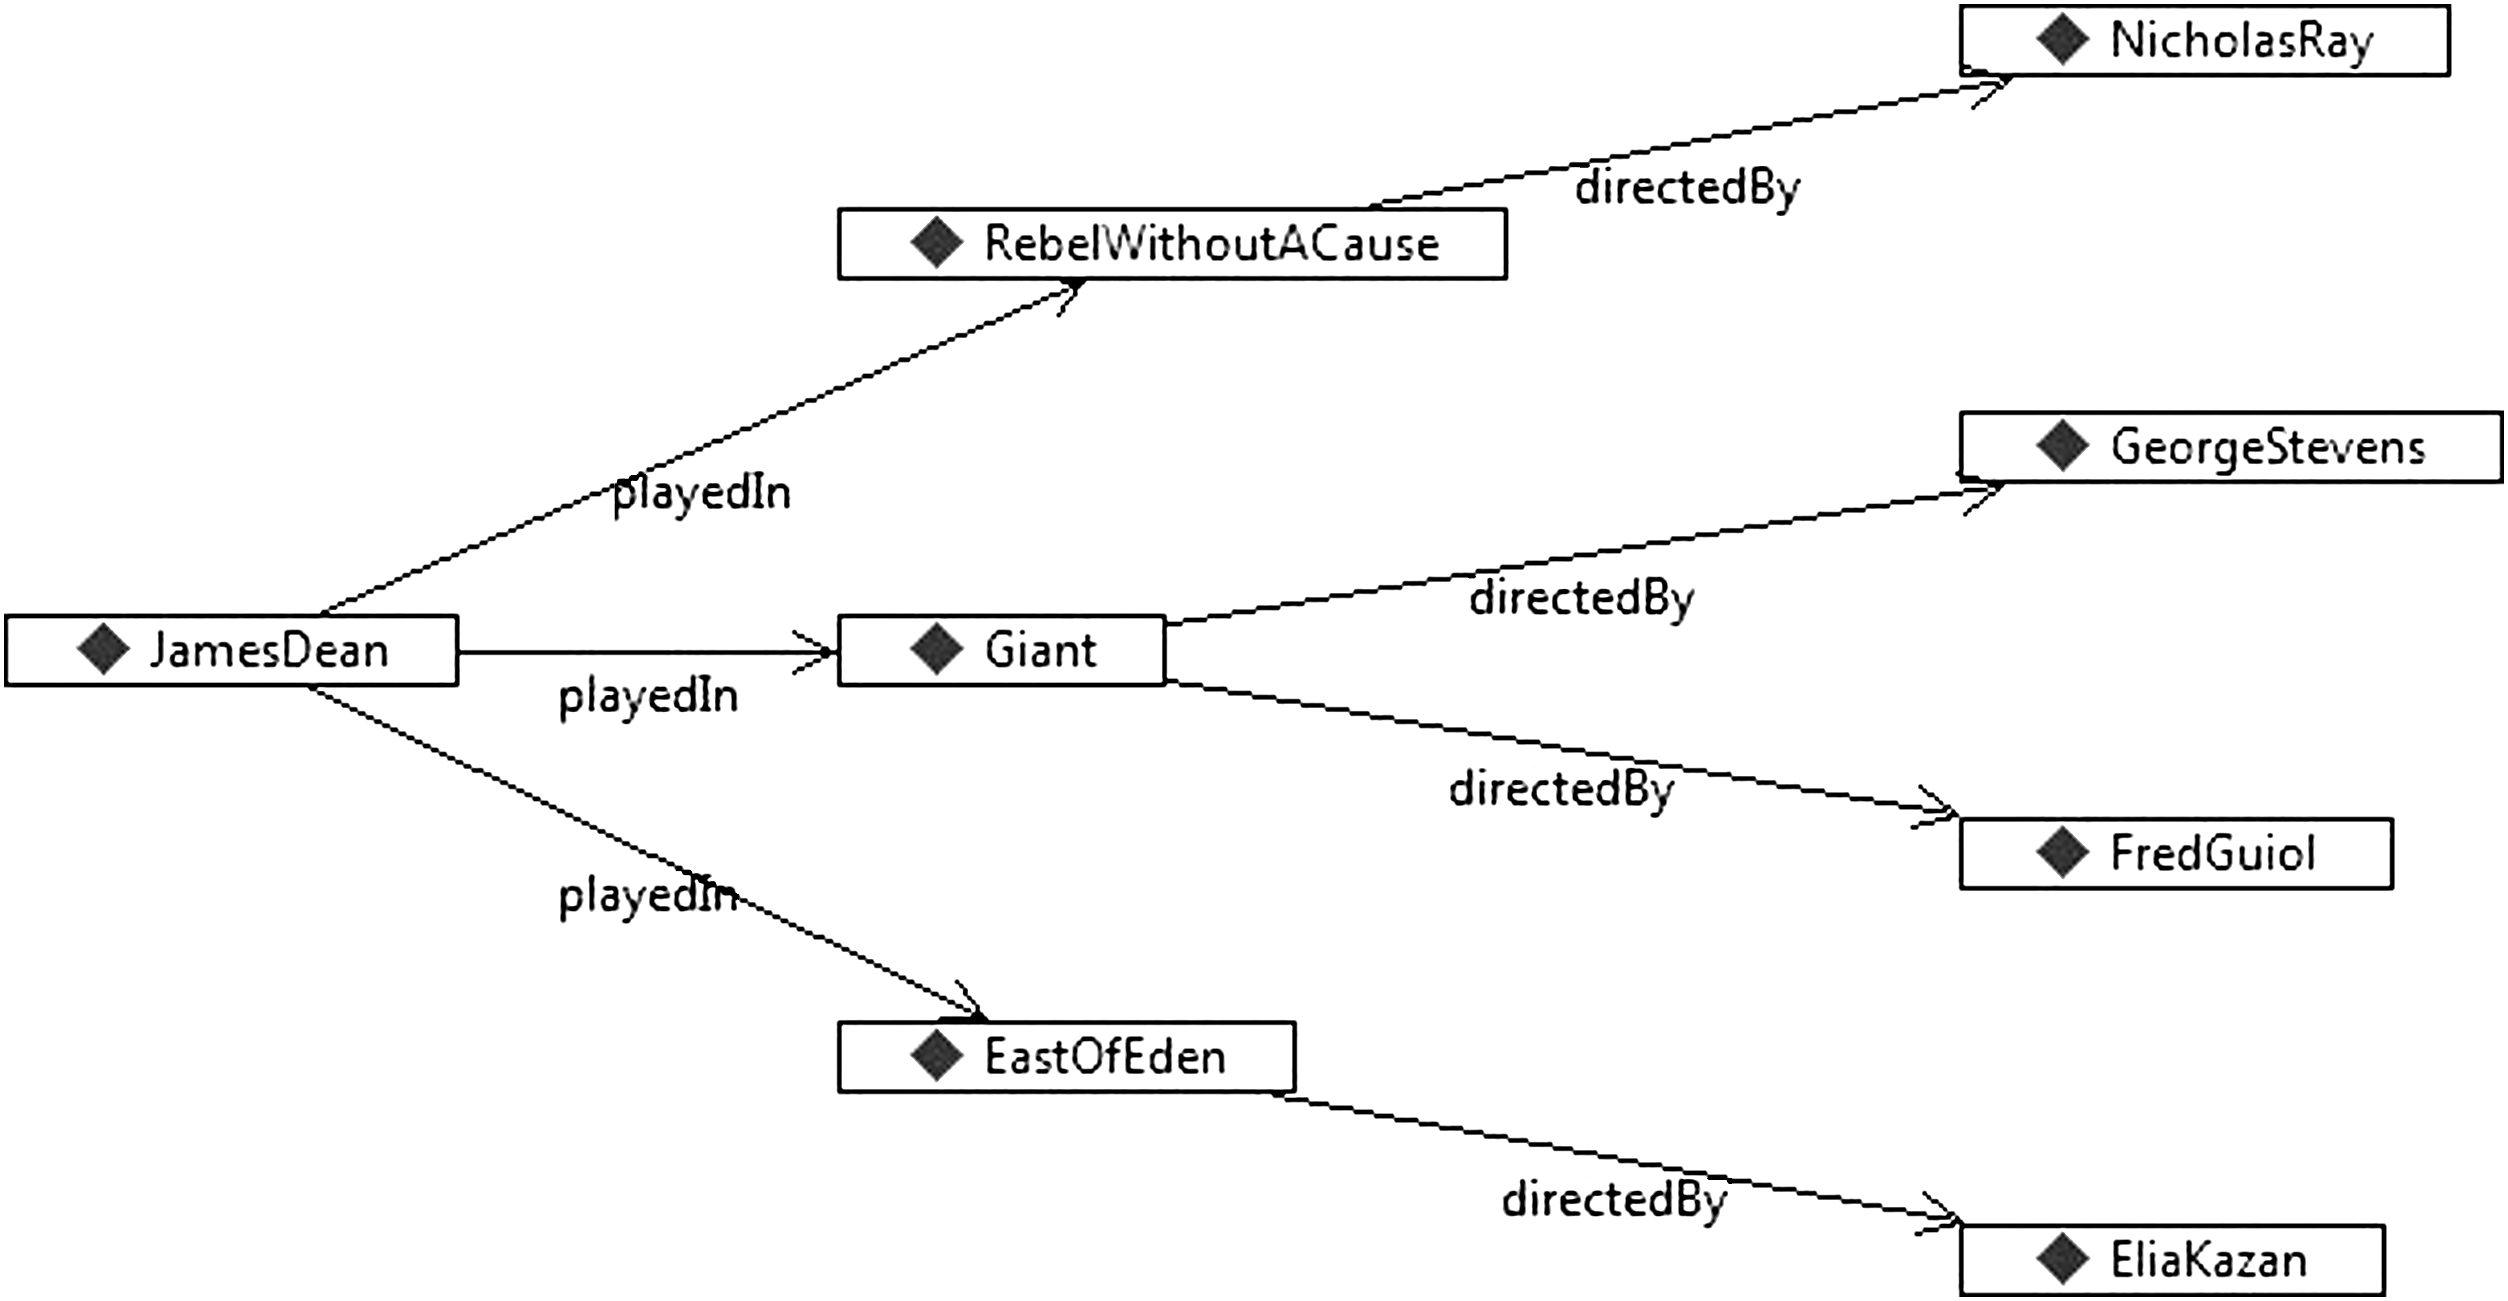
\includegraphics[width=5in]{media/f06-02.png}
\label{fig:ch6.2}
\caption{James Dean's movies and their directors.}
\end{figure}

\begin{figure}
\centering
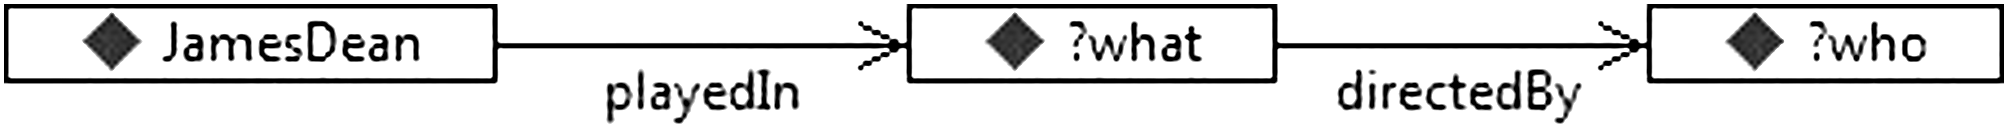
\includegraphics[width=5in]{media/f06-03.png}
\label{fig:ch6.3}
\caption{Graphic version of a query to find James Dean's directors.}
\end{figure}

James Dean worked with? We can query this by asking who directed the
movies that James Dean played in. The graph pattern for this query has
two triples:

\begin{lstlisting}
:JamesDean :playedIn ?what .
?what :directedBy ?who .
\end{lstlisting}

Since the variable \texttt{?what} appears in both triples, the graph pattern is
joined at that point. We can draw a graph pattern the same way we draw a
graph. Figure 5.3 shows this graph pattern. There are two triples in the
pattern and two triples in the diagram.

This graph pattern has two question words, so the query engine will find
all matches for the pattern, with both question words being free to
match any resource. This results in several matches:

\begin{tabular}{ l l }
?what=:Giant&?who=:GeorgeStevens\\
?what=:Giant&?who=:FredGuiol \\
?what=:EastOfEden&?who=:EliaKazan \\
?what=:RebelWithoutaCause&?who=:NicholasRay \\
\end{tabular}

When we have more than one question word, we might actually only be
interested in one of them. In this case, we asked what directors James
Dean had worked with; the movies he played in were just a means to that
end. This is where the details of the SELECT clause come in -- we can
specify which question words we are interested in. So the complete query
to find James Dean's directors looks like this:

\textbf{\textbf{Ask:}}

\begin{lstlisting}
SELECT ?who
WHERE {:JamesDean :playedIn ?what .
       ?what :directedBy ?who . }
\end{lstlisting}

\textbf{\textbf{Answer:}}

\begin{lstlisting}
:GeorgeStevens, :EliaKazan, :NicholasRay, :FredGuiol
\end{lstlisting}

Since a query in SPARQL can have several question words and several
answers, it is convenient to display the answers in a table with one
column for each question word and one row for each answer.

\begin{tabular}{|l|}
\hline
?who\\
\hline
:GeorgeStevens\\
:EliaKazan\\
:NicholasRay\\
:FredGuiol\\
\hline
\end{tabular}

If we decide to keep both question words in the SELECT, we will have
more columns in the table

\textbf{\textbf{Ask:}}

\begin{lstlisting}
SELECT ?what ?who
WHERE {:JamesDean :playedIn ?what .
       ?what :directedBy ?who .}
\end{lstlisting}

\begin{tabular}{| l l | }
\hline
?what&?who\\
\hline
:Giant&:GeorgeStevens\\
:Giant&:FredGuiol\\
:EastOfEden&:EliaKazan\\
:RebelWithoutaCause&:NicholasRay\\
\hline
\end{tabular}

\subsection{Naming question words in SPARQL}

In English, we have a handful of question words -- who, what, where,
etc. A question doesn't make sense if we use some other word. But in
SPARQL, a question word is just signaled by the ? at the start -- any
word would do just as well. If we look at the output table above, the
question words \texttt{?who} and \texttt{?what} are not very helpful in describing what is
going on in the table. If we remember the question, we know what they
mean (\texttt{?what} is a movie, and \texttt{?who} is its director). But we can make the
table more understandable, even out of the context of the question, by
selecting descriptive question words. It is customary in SPARQL to do
this, to communicate the intention of a question word to someone who
might want to read the query. For example, we might write this query as

\textbf{\textbf{Ask:}}

\begin{lstlisting}
SELECT ?movie ?director
WHERE {:JamesDean :playedIn ?movie .
       ?movie :directedBy ?director .}
\end{lstlisting}

\textbf{\textbf{Answer:}}

\begin{tabular}{|ll|}
\hline
?movie&?director\\
\hline
:Giant&:GeorgeStevens\\
:Giant&:FredGuiol\\
:EastOfEden&:EliaKazan\\
:RebelWithoutaCause&:NicholasRay\\
\hline
\end{tabular}

The graph pattern we just saw was a simple chain -- James Dean played in
some movie that was directed by someone. Graph patterns in SPARQL can be
as elaborate as the graphs they match against. For instance, given a
more complete set of information about James Dean movies we could find
the actresses who worked with him with a graph pattern:

\textbf{\textbf{Ask:}}

\begin{lstlisting}
SELECT ?actress ?movie
WHERE {:JamesDean :playedIn ?movie .
       ?actress :playedIn ?movie .
       ?actress rdf:type :Woman }
\end{lstlisting}

\textbf{\textbf{Answer:}}

\begin{tabular}{|l|}
\hline
?actress\\
\hline
:AnnDoran\\
:ElizabethTaylor\\
:CarrollBaker\\
:JoVanFleet\\
:JulieHarris\\
:MercedesMcCambridge\\
:NatalieWood\\
\hline
\end{tabular}

Figure~\ref{ch5.4} shows a fragment of the data graph, and the graph pattern,
with the result for the question word \texttt{?actress} indicated in the third
`column' of the figure. Notice that Rock Hudson is not a match; while he
indeed played in \emph{Giant}, there is no match for the third triple,

\begin{lstlisting}
:RockHudson rdf:type :Woman.
\end{lstlisting}

\begin{figure}
\centering
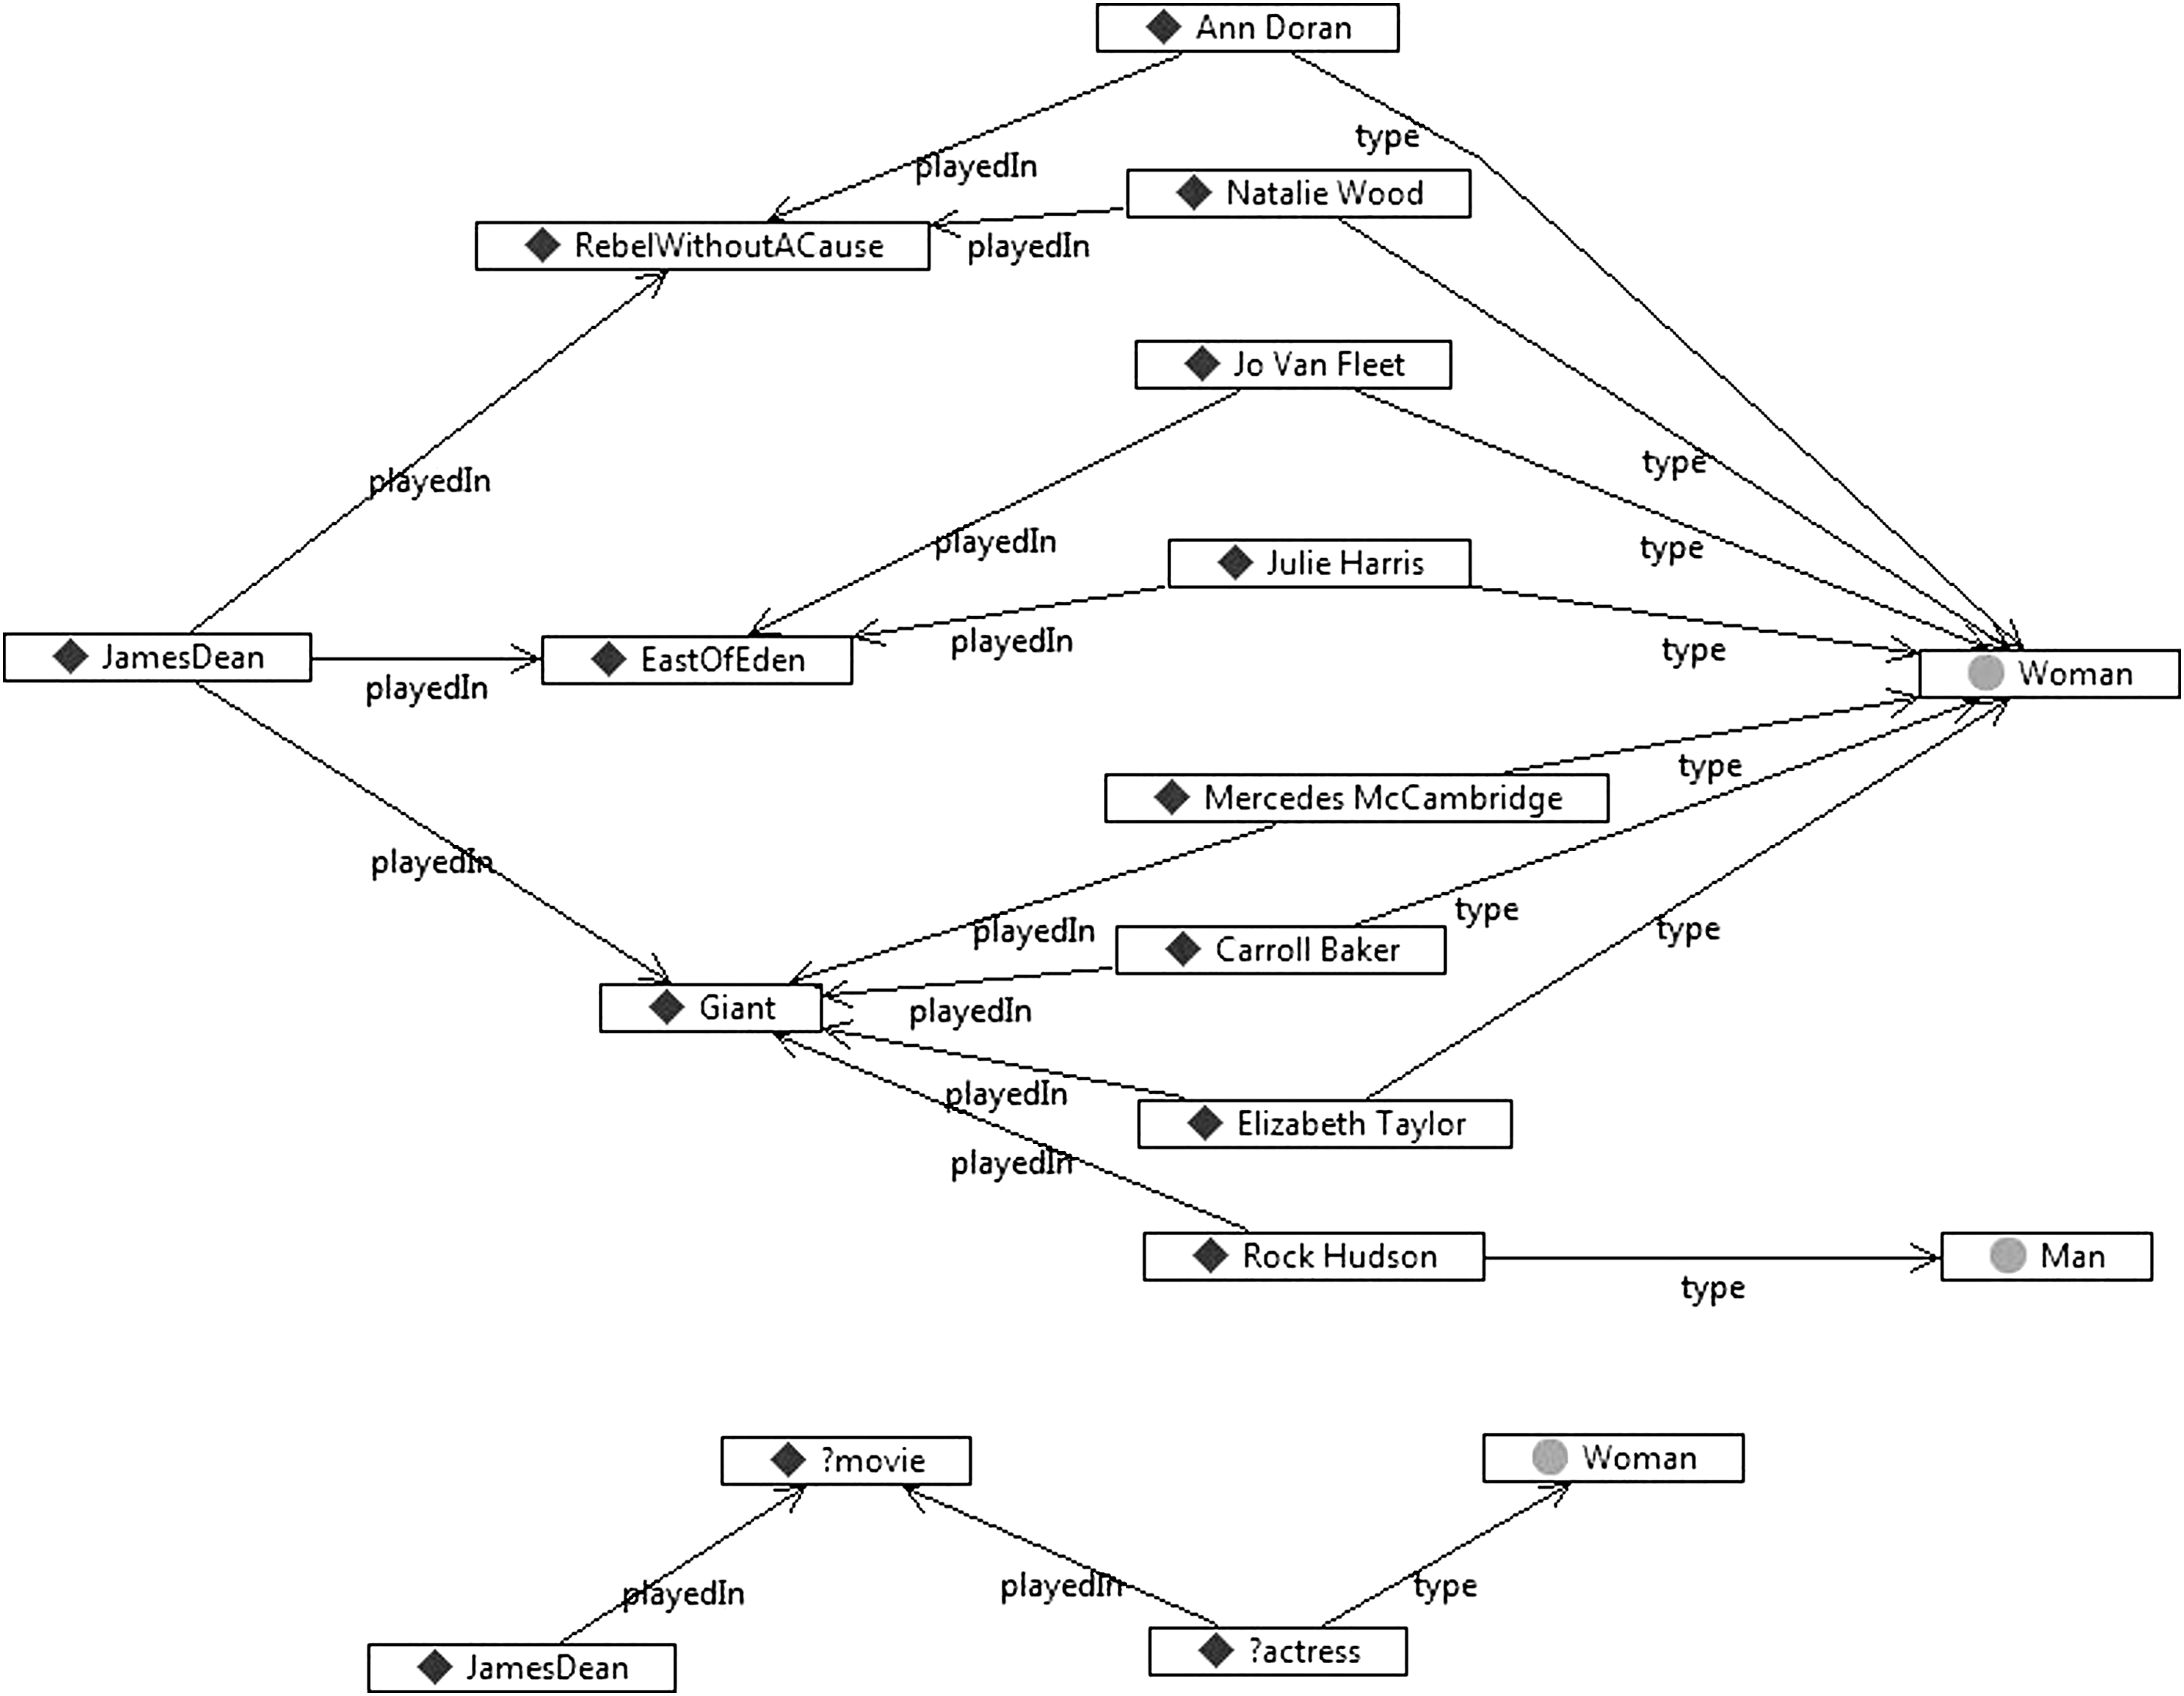
\includegraphics[width=5in]{media/f06-04.png}
\label{fig:ch6.4}
\caption{Information about James Dean's co-stars, and a query to fetch some of it.}
\end{figure}

Remember that \texttt{?actress} is just a question word like \texttt{?who}, renamed to be
more readable; the only reason \texttt{?actress} doesn't match \texttt{:RockHudson} is
because the data do not support the match. That is, the meaning of
\texttt{?actress} is not given by its name, but instead by the structure of the
graph pattern.

With this observation, one might wonder how we know that \texttt{?movie} is sure
to come up with movies? And indeed, this is a consideration; in this
example, the only things that James Dean played in were movies, so it
really isn't an issue. But on the Semantic Web, we could have more
information about things that James Dean played in. So we really should
restrict the value of the question word \texttt{?movie} to be a member of the
class movie. We can do this by adding one more triple to the pattern:

\textbf{\textbf{Ask:}}

\begin{lstlisting}
SELECT ?actress
WHERE {:JamesDean :playedIn ?movie .
       ?movie rdf:type :Movie .
       ?actress :playedIn ?movie .
       ?actress rdf:type :Woman  }
\end{lstlisting}

This query pattern is shown graphically in Figure\ref{fig:ch6.5}. Triples like

\begin{lstlisting}
?movie rdf:type :Movie .
\end{lstlisting}

can seem a bit confusing at first -- with two uses of the word movie,
what does this mean? But now that we know that \texttt{?movie} is just a generic
question word with a name that prints well in a table, we can see that
this triple is how we tell SPARQL what we really mean by \texttt{?movie}. The
meaning isn't in the name, so we have to put it in a triple.

You might come upon a model that gives properties the same name as the
class of entity they are intended to point to -- so that instead of a
property called \texttt{:directedBy} in this example, a model might call it
simply \texttt{:director}. In such a case, the query to find the people who
directed James Dean movies would look like this:

\begin{lstlisting}
SELECT ?director
WHERE {:JamesDean :playedIn ?movie .
       ?movie :director ?director .}
\end{lstlisting}

\begin{figure}
\centering
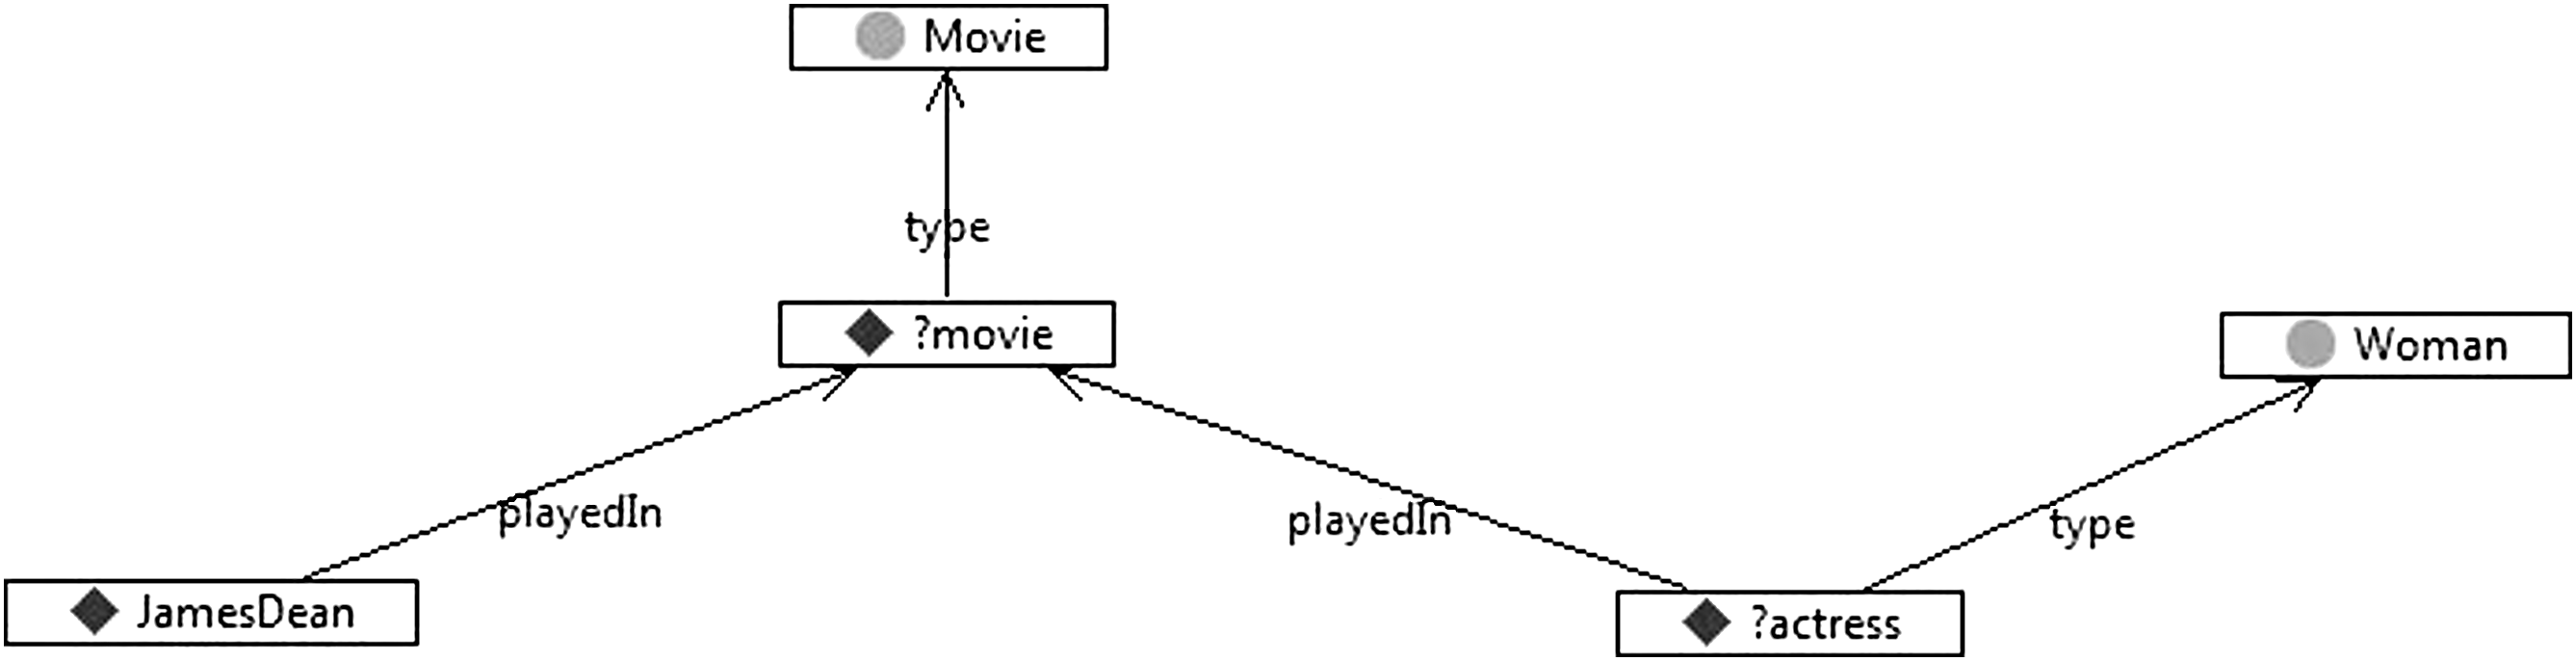
\includegraphics[width=5in]{media/f06-05.png}
\label{fig:ch6.5}
\caption{Extended query pattern that includes the fact that ?movie has type Movie.
}
\end{figure}

This can look a bit daunting -- what is the difference between \texttt{?director}
and \texttt{:director}? As we've already seen, \texttt{:director} refers to a particular
resource (using the default namespace -- that's what the ``:'' means) On
the other hand, \texttt{?director} is a question word -- it could have been \texttt{?foo}
or \texttt{?bar} just as easily, but we chose \texttt{?director} to remind us of its
connection with a movie director, when we see it out of the context of
the query. If you have to write (or read!) a query written for a model
that names its properties in this way, don't panic! Just remember that
the ? marks a question word -- the name \texttt{?director} is just there to let
you (and whoever else reads the query) know what \texttt{?director} is expected
to mean. If you are creating your own model, we recommend that you use
property names like \texttt{:directedBy} instead of \texttt{:director} so that you don't
invite this confusion in the people who want to query data using your
model.

\subsection{Query structure vs. data structure}

In Figure\ref{fig:ch6.4}, we saw how the graph pattern in a query looks a lot like
the data graph it matches against. This is true of graph patterns in
general. The complexity of a question that can be specified with SPARQL
is limited only by the complexity of the data. We could, for instance,
ask about actresses who played in a movie with James Dean who themselves
were in a movie directed by John Ford:

\textbf{\textbf{Ask:}}
\begin{lstlisting}
SELECT ?actress ?movie
WHERE {:JamesDean :playedIn ?movie .
       ?actress :playedIn ?movie .
       ?actress a :Woman .
       ?actress :playedIn ?anotherMovie .
       ?anotherMovie :directedBy :JohnFord .}
\end{lstlisting}

\textbf{\textbf{Answer:}}

\begin{tabular}{|l|}
\hline
?actress\\
\hline
NatalieWood\\
CarrollBaker\\
\hline
\end{tabular}

Figure\ref{fig:ch6.6} shows this query as a graph. In the text version of the
query, we often see the same question word appear in multiple triples,
and some of them even refer to the same kind of thing (\texttt{?movie},
\texttt{?anotherMovie}). In the graph version, we see that these are the points
where two triples must refer to the same thing. For instance, we know
that James Dean and \texttt{?actress} played in the same movie, because both
triples use the same question word (\texttt{?movie}) for that movie. Similarly,
that \texttt{?actress} is the same one who played in \texttt{?anotherMovie}, because there
the same question word \texttt{?actress} appears in those two triples. All these
relationships are visibly apparent in Figure\ref{fig:ch6.6}, where we see that
\texttt{?movie} is the connection between James Dean and \texttt{?actress}, \texttt{?actress} is
the connection between \texttt{?movie} and \texttt{?anotherMovie}, and \texttt{?anotherMovie} is
the connection between \texttt{?actress} and John Ford.

If we look at the information supporting the answer ``Natalie Wood,'' we
see that the data graph looks just like the graph pattern -- this should
come as no surprise, since that is how the pattern works. But we can use
this feature to our advantage when writing queries. One way to write a
complex query like the one in Figure\ref{fig:ch6.6} is to walk through the question
we want to answer, writing down triples as we go until we have the full query. But another way is to start with the
data. Suppose we have an example of what we want to search for, for
example, we know that Natalie Wood played in The Searchers, which was
directed by John Ford. Next, we show how we can use the close match
between graphs and patterns to construct the pattern from the example.


\begin{figure}
\centering
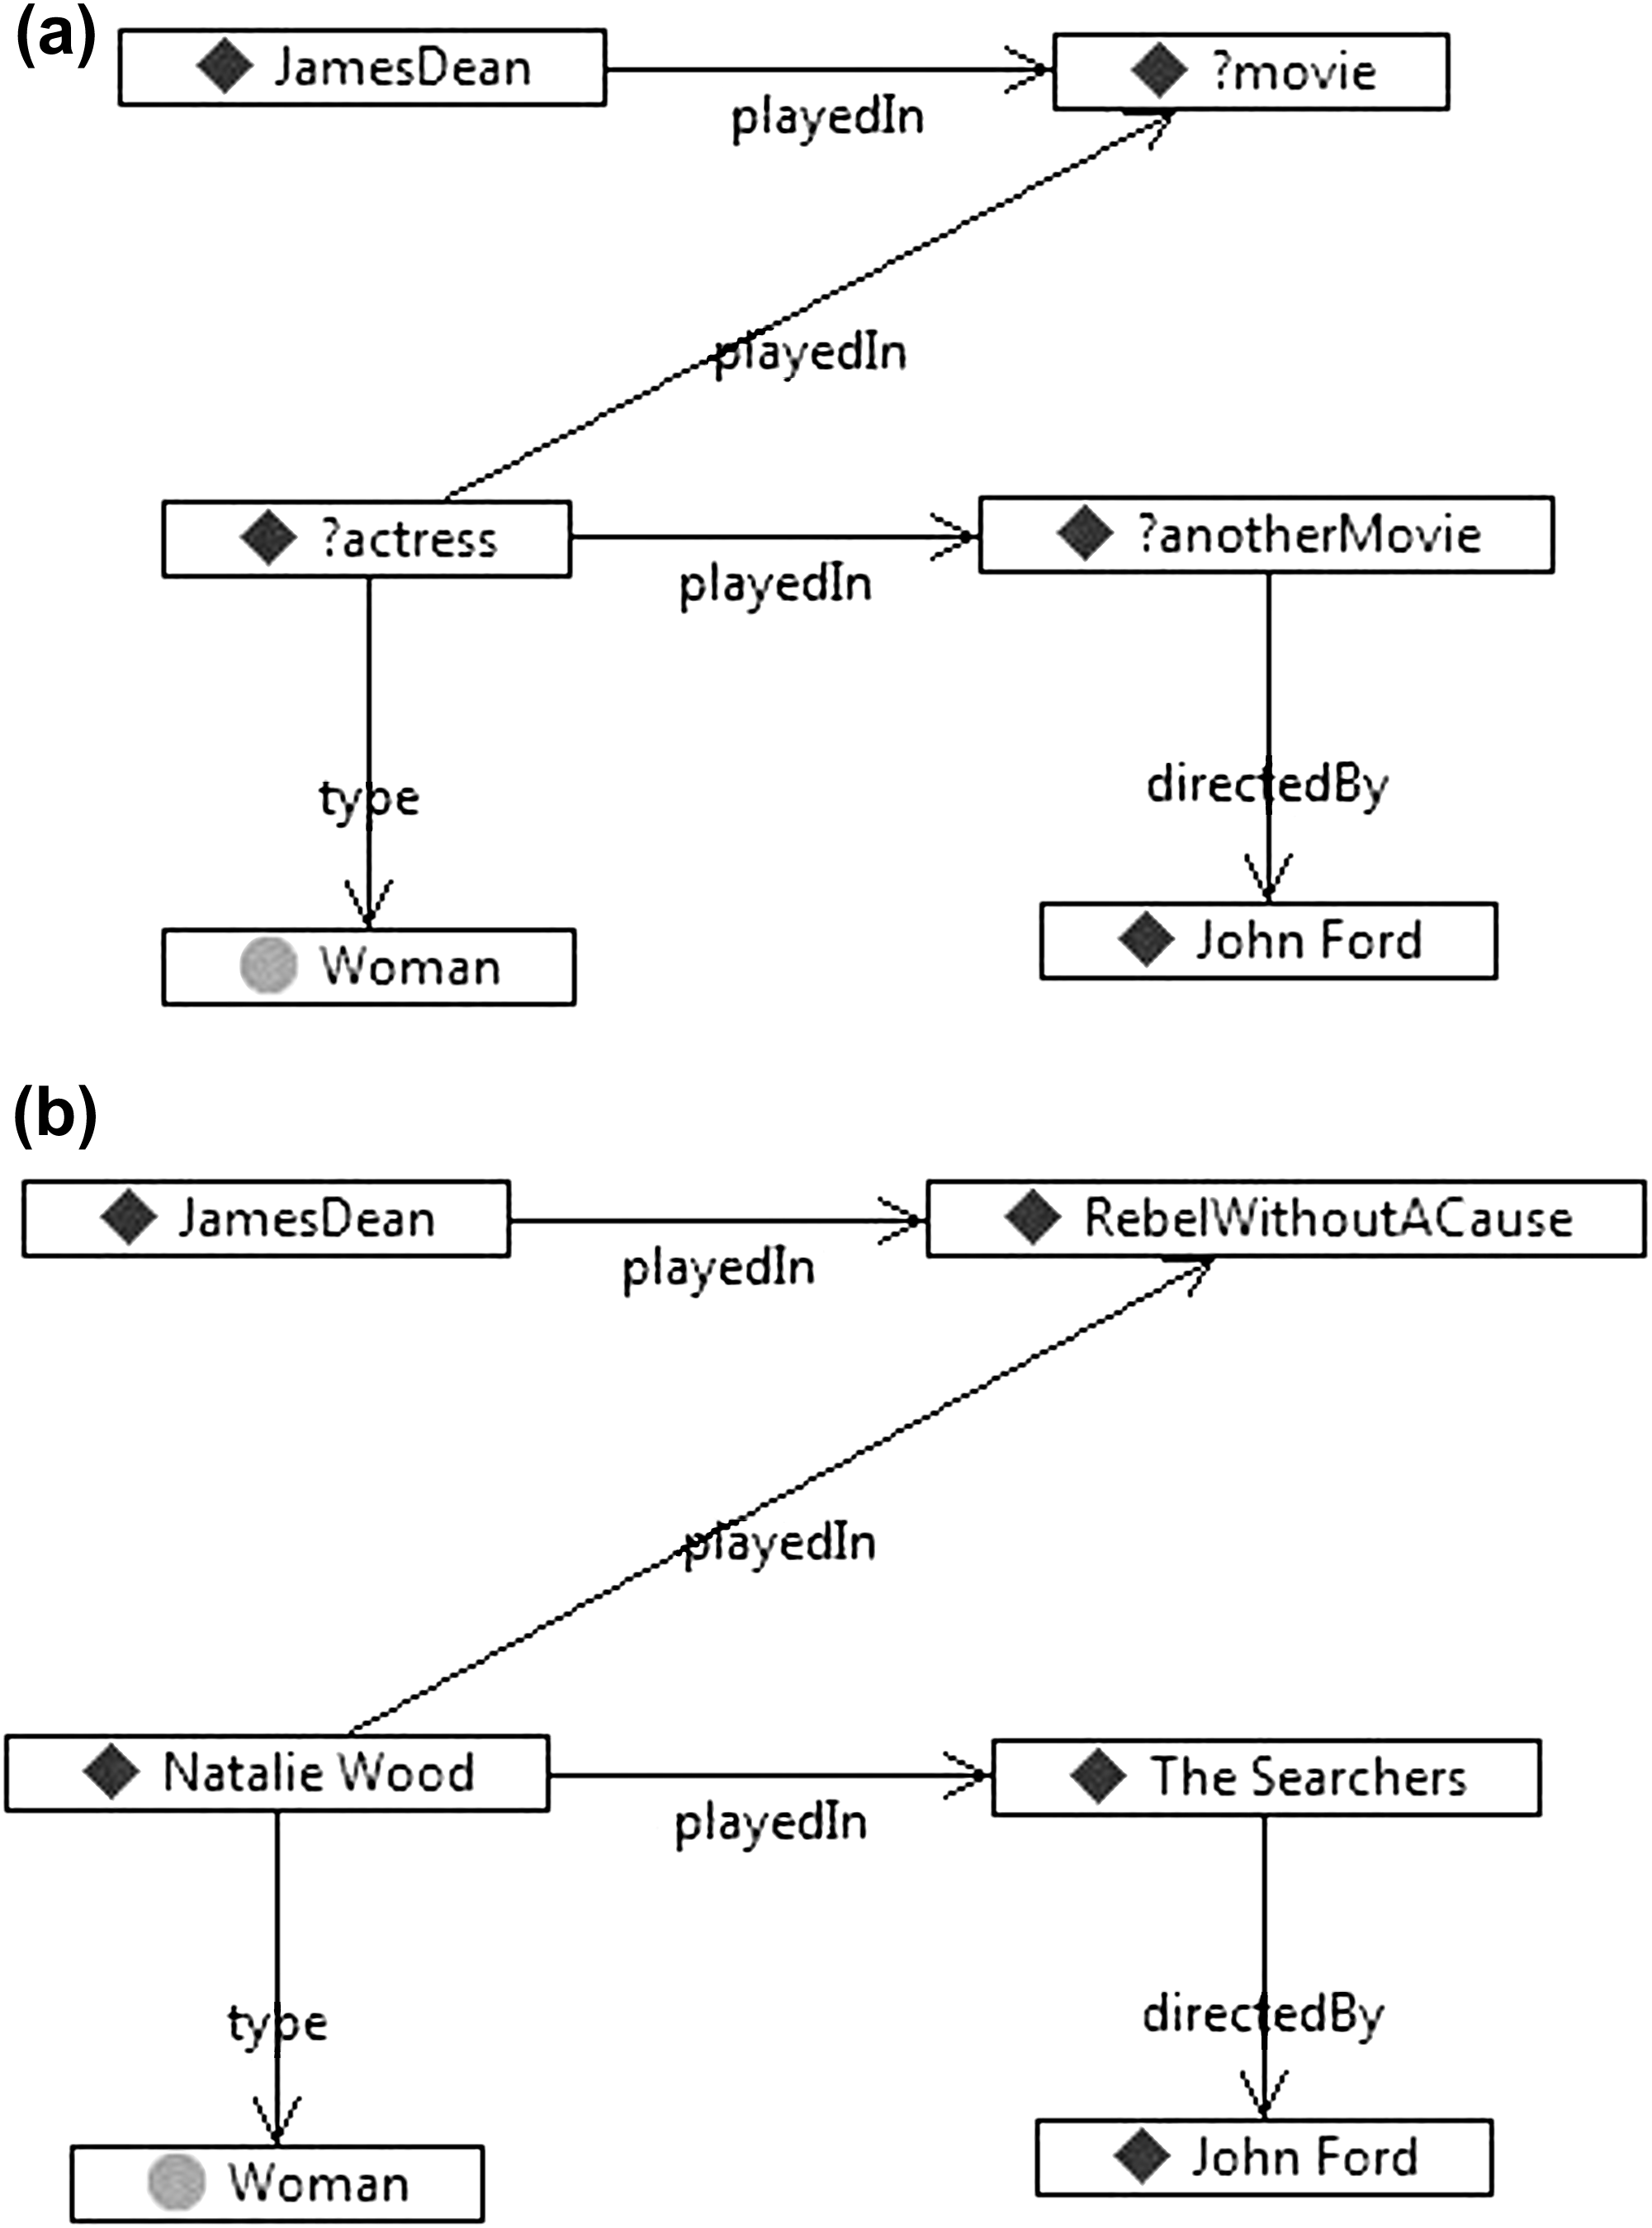
\includegraphics[width=5in]{media/f06-06.png}
\label{fig:ch6.6}
\caption{Data about James Dean and Natalie Wood, and a query to fetch that data.}
\end{figure}


Since the example from the data graph matches the graph pattern triple
for triple, we already know a lot about the graph pattern we want to
create. The only thing we need to specify is which values from the
example we want to keep as literal values in the pattern, and which ones
we want to replace with
question words. In Figure\ref{fig:ch6.7}(a) the boxed x on certain resources (James
Dean, John Ford, and Woman) indicates those that will stay as they are;
all other resources (Natalie Wood, The Searchers, \emph{Rebel without a
Cause}) will be replaced with question words. We have to decide what
question words to use; there could be a lot of them. Remember that as
far as the SPARQL query engine is concerned, the names of the question
words aren't important, so we can call them whatever we like as long as
we make sure to use the same question word when we need the same value
to be used in the answer. For this example, we'll call them \texttt{?q1}, \texttt{?q2},
etc. Figure\ref{fig:ch6.7}(b) shows the query pattern graphically.

\begin{figure}
\centering
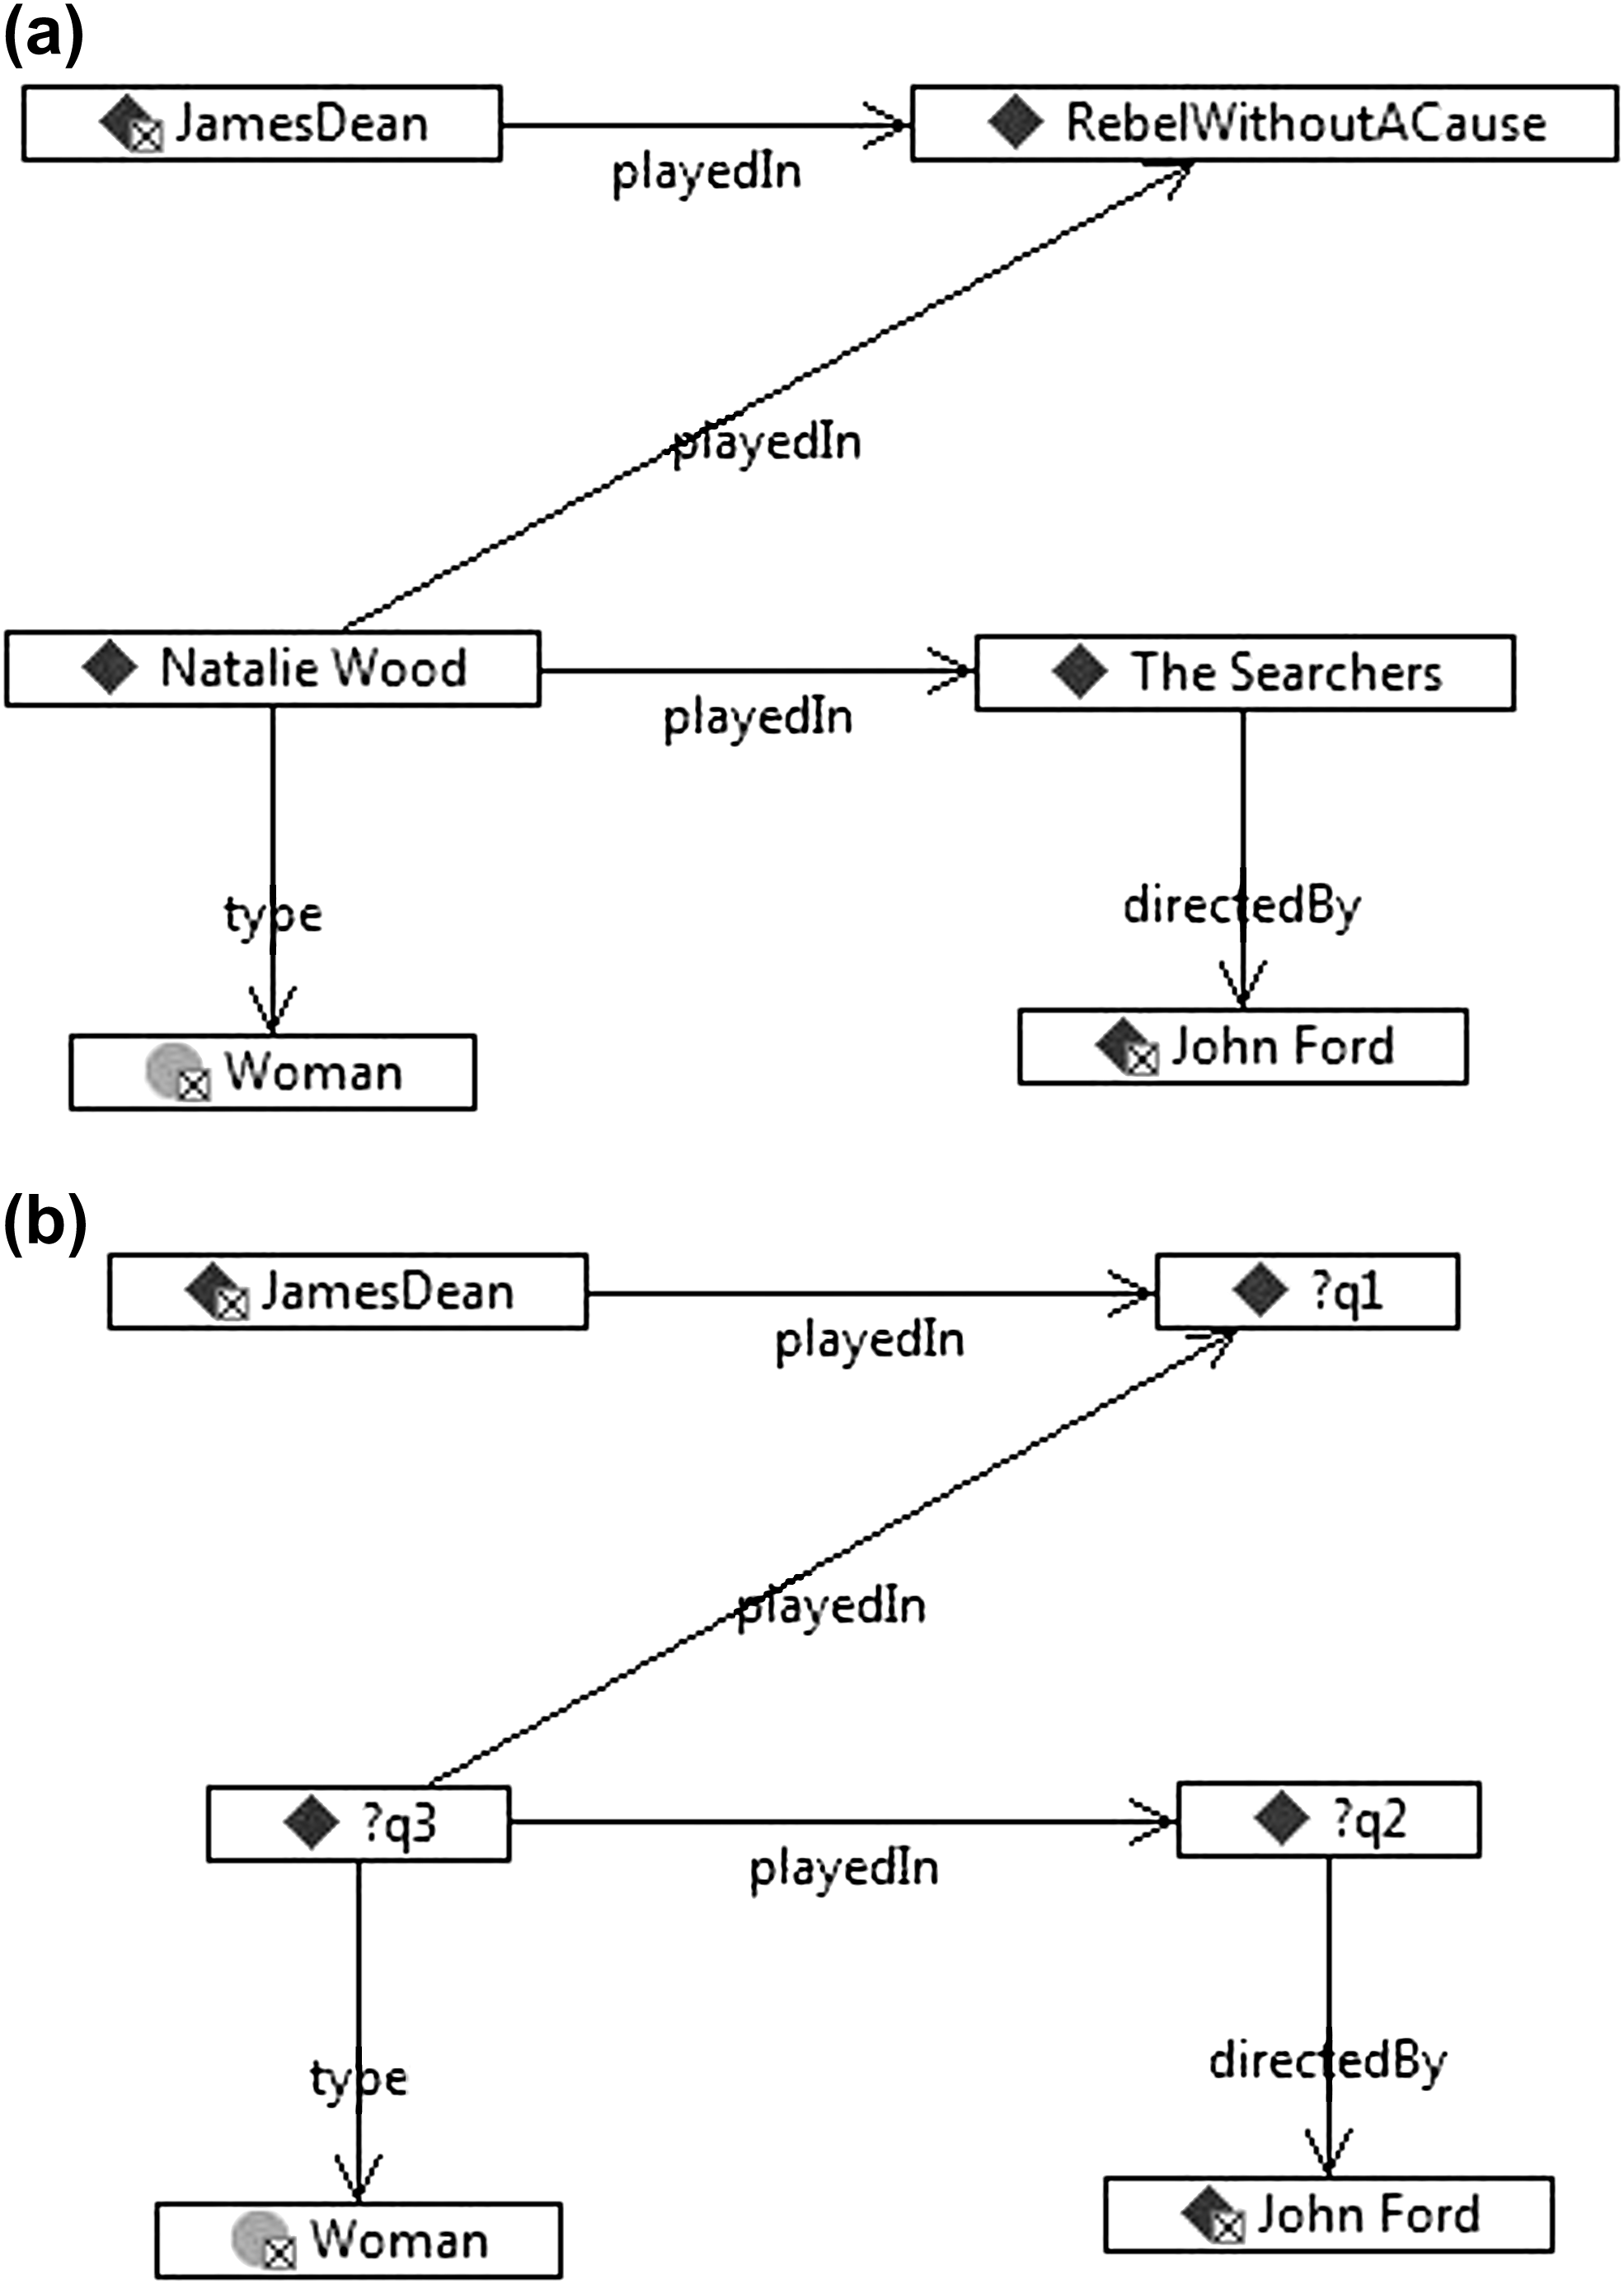
\includegraphics[width=5in]{media/f06-07.png}
\label{fig:ch6.7}
\caption{Creating a graph pattern from a data graph. Resources marked with X appear as themselves in the query.}
\end{figure}


Now we can create our SPARQL query by simply copying down the graph
pattern in Turtle. Each arrow in the graph becomes a triple. If a
particular entity (either a literal resource or a question word)
participates in more than one triple in the graph, then it will appear
more than one time in the Turtle rendering of the pattern. The graph
diagram in Figure\ref{fig:ch6.7}(b) has five connecting arrows; the corresponding
query will have the same number of triples:

\begin{lstlisting}
{ :JamesDean :playedIn ?q1 .
   ?q3 :playedIn ?q1 .
   ?q3 rdf:type :Woman .
   ?q3 :playedIn ?q2 .
   ?q2 :directedBy :JohnFord .}
\end{lstlisting}

To complete the query, simply SELECT the question word(s) you want to
report on, and perhaps give it a meaningful name. This brings us back to
a query very like the original query (differing only in the names of the
unselected question words) -- but this time, it was generated from a
pattern in the data.

\begin{lstlisting}
SELECT ?actress
WHERE {:JamesDean :playedIn ?q1 .
       ?actress :playedIn ?q1 .
       ?actress rdf:type :Woman .
       ?actress :playedIn ?q2 .
       ?q2 :directedBy :JohnFord . }
\end{lstlisting}


As we saw above, there are two matches for this query in the sample
data, Natalie Wood (no surprise there -- after all, it was her
performance that we used as a model for this query) and Carroll Baker.
Carroll Baker is similar to Natalie Wood, in that she is also a woman,
she also played alongside James Dean in a movie, and she was also
directed by John Ford. She is similar to Natalie Wood in exactly the
features specified in the query.

This method for creating queries can be seen as a sort of ``more like
this'' capability; once you have one example of something you are
interested in, you can ask for ``more like this,'' where the notion of
``like this'' is made specific by including particular triples in the
example, and hence in the graph pattern.

For example, we just wrote a query that found actresses who played in
James Dean movies and also played in movies directed by John Ford. How
do we know that the results are limited to actresses? In the example,
Natalie Wood is an actress. But she is one of the resources that we
replaced by a question word -- how do we know that all the things that
the pattern matches will also be actresses? We know this because we
included the triple

\begin{lstlisting}
?q3 rdf:type :Woman .
\end{lstlisting}

in the example, and hence in the pattern.

What would happen if we left that triple out? Natalie Wood is, of
course, still a Woman in the data graph, but we haven't included that
fact in our example. So that fact does not get copied into the query.
Our new query looks like this:

\begin{lstlisting}
SELECT ?q3
WHERE { :JamesDean :playedIn ?q1 .
        ?q3 :playedIn ?q1 .
        ?q3 :playedIn ?q2 .
        ?q2 :directedBy :JohnFord . }
\end{lstlisting}

It has one fewer triple than the previous query. What is the difference
if we run this query against the data? Now we get another answer --
Raymond Massey (who also played in \emph{East of Eden}). It would be
misleading (but perfectly fine from the point of view of the SPARQL
query language) to name this question word \texttt{?actress} in this situation --
we might want to call it \texttt{?actor} instead (with the convention that women
can also be actors; if we don't like that convention, we might just keep
the meaningless name \texttt{?q3}).

So when we say we want to match ``more like this'' from the example of
Natalie Wood, in the first case, we meant ``Women who played with James
Dean in some movie, and who played in a movie directed by John Ford.''
In the second case, we just asked for ``Anyone (even anything) who
played with James Dean in some movie, and who played in a movie directed
by John Ford.'' How did we specify the difference? By including (or
excluding) the triple that asserts that Natalie Wood is a woman. When we
include it, ``more like this'' includes the fact that the result must be
a Woman. When we exclude it, ``more like this'' does not include this
stipulation.

\subsection{Ordering of triples in SPARQL queries}

In the previous section, we copied down a graph pattern that was
expressed in graphical form into Turtle. The process was straightforward
-- for each triple in the graph (i.e., each arrowhead), write down one
triple in Turtle. But this process left out one variation -- in what
order do you write down the triples?

One of the beauties of the RDF data model is that its semantics are
specified by the graph -- the order in which triples are written down
makes no difference to an RDF data graph. This is
also true for a graph pattern. To be specific, a graph pattern written
in one order will produce the same results (when matched against the
same data graph) as another graph pattern, with all the same triples,
written in a different order. This means that, as far as the pattern
matches are concerned, it makes no difference what order the triples are
written in; the graph pattern is the same either way.

\subsection{Querying for properties and schema}

In all of our examples so far, we have written out each triple in the pattern, one triple per line.  
But SPARQL is based on the same syntax as Turtle (chapter~\ref{ch3}, where we can use semicolons and commas as shortcuts
in writing triples; we'll start using those shortcuts from now on.  Not only do they make the queries shorter, they
tend to be more readable as well. 

In our examples so far, 
we have also used question words only for the
subjects and objects of triples. But the SPARQL pattern matching
paradigm allows predicates to be matched as well.

A simple exploitation of this is to answer the question, ``What do you
know about James Dean?'' This can be done with a graph pattern of a
single triple:

\textbf{\textbf{Ask:}}

\begin{lstlisting}
SELECT ?property ?value
WHERE { :JamesDean ?property ?value }
\end{lstlisting}

\textbf{\textbf{Answer:}}

\begin{tabular}{|ll|}
\hline
?property&?value\\
\hline
bornOn&1931-02-\\
diedOn&1955-09-30\\
playedIn&RebelWithoutaCause\\
layedIn&EastOfEden\\
playedIn&\emph{Giant}\\
rdf:type&Man\\
rdfs:label&James Dean\\
\hline
\end{tabular}


This is a powerful feature for exploring data sets that you aren't very
familiar with. And since we are on the Semantic Web, that is likely to
happen frequently. You might not know what properties are defined for
James Dean, but this query will find them for you, and show you the
values.

You don't have to ask for the values -- you can just ask for the
properties. This will tell you what sort of information is available,
without reporting all of the details:

\textbf{\textbf{Ask:}}

\begin{lstlisting}
SELECT ?property
WHERE { :JamesDean ?property ?value }
\end{lstlisting}

\textbf{\textbf{Answer:}}

\begin{tabular}{|l|}
\hline
?property\\
\hline
bornOn\\
diedOn\\
playedIn\\
playedIn\\
playedIn\\
rdf:type\\
rdfs:label\\
\hline
\end{tabular}

This query effectively asks for metadata about James Dean -- it is
asking, ``what are the sorts of things this dataset knows about James
Dean?''

Notice that the result \texttt{:playedIn} appears three times in the answers.
This is because there are actually three different matches for the graph
pattern in the data graph. SPARQL includes the keyword DISTINCT to
filter out the duplicate results.

\textbf{\textbf{Ask:} }

\begin{lstlisting}
SELECT DISTINCT ?property
WHERE {  :JamesDean ?property ?value  }
\end{lstlisting}

\textbf{\textbf{Answer:} }

\begin{tabular}{|l|}
\hline
?property\\
\hline
bornOn\\
diedOn\\
playedIn\\
rdf:type\\
rdfs:label\\
\hline
\end{tabular}

This ability to query for properties used in the data distinguishes
SPARQL from many other query languages. Among other things, this makes
it possible to reverse-engineer schema information from the data itself.
For example, we can change the query about properties used to describe
James Dean to find all properties used to describe any actor.

\textbf{\textbf{Ask:}}

\begin{lstlisting}
SELECT DISTINCT ?property
WHERE {?q0 a :Actor .
       ?q0 ?property ?object .}
\end{lstlisting}

\textbf{\textbf{Answer:}}

\begin{tabular}{|l|}
\hline
?property\\
\hline
bornOn\\
diedOn\\
playedIn\\
rdf:type\\
rdfs:label\\
produced\\
sang\\
wrote\\
\hline
\end{tabular}

What if we don't know about the class \texttt{:Actor}? We can ask about that as
well:

\textbf{\textbf{Ask:}}

\begin{lstlisting}
SELECT DISTINCT ?class
WHERE { ?class rdfs:subClassOf :Person }
\end{lstlisting}

\textbf{\textbf{Answer:}}

\begin{tabular}{|l|}
\hline
?class\\
\hline
:Actor\\
:Actress\\
:Man\\
:Woman\\
:Politician\\
:Producer\\
\hline
\end{tabular}

If we don't know anything about the data at all, we can find the classes
used in the data

\begin{lstlisting}
SELECT DISTINCT ?class
WHERE { ?q0 a ?class }
\end{lstlisting}

Or find all the properties used anywhere in the data

\begin{lstlisting}
SELECT DISTINCT ?property
WHERE { ?q0 ?property ?q1 }
\end{lstlisting}

Queries of this sort take advantage of a number of distinctive features
of RDF; first, that it is possible to match any part of the data
(subjects, predicates, objects) with a question word, and that RDFS, the
schema language of RDF (Chapter 8), is also expressed in RDF. These two
features of RDF/SPARQL make RDF ``self-describing'' in a way that goes
beyond most representation languages.

\subsection{Variables, bindings, and filters}

In the last example, we showed how we can use DISTINCT to remove some
rows from the result set. We can use this idea to pose more detailed
questions using SPARQL.

James Dean and many of his co-stars died very young, while others
enjoyed long lives and careers. We might want to find out which of the
actors who played in \emph{Giant} lived for more than five years after
the movie was made. We'll start by finding the date of death of every
actor in \emph{Giant} with the query:

\textbf{\textbf{Ask:}}

\begin{lstlisting}
SELECT ?actor ?deathdate
WHERE { ?actor :playedIn :Giant ;
               :diedOn ?deathdate .}
\end{lstlisting}

\textbf{\textbf{Answer:}}

\begin{tabular}{|ll|}
\hline
Actor&deathdate\\
\hline
RockHudson&1985-10-02\\
JamesDean&1955-10-30\\

\hline
\end{tabular}


This is useful information, and the answer lies in the table, but the
query hasn't really answered our question -- who lived on past November
24, 1961 (five years after the production date of \emph{Giant})?

You can define your own conditions under which rows will be excluded
from the results, using the keyword FILTER. The idea of FILTER is that
you can define a Boolean test that determines whether that row will be
included in the results or not. We can filter out the names of the
actors who lived on by adding a FILTER to the query, as follows:

\textbf{\textbf{Ask:}}

\begin{lstlisting}
SELECT ?actor
WHERE { ?actor :playedIn :Giant ;
               :diedOn ?deathdate . 
        FILTER (?deathdate  "1961-11-24"^{^{xsd:date) }
\end{lstlisting}

\textbf{\textbf{Answer:}}

\begin{tabular}{|l|}
\hline
Actor\\
\hline
RockHudson\\
\ldots\\
\hline
\end{tabular}


So far, we have referred to things like \texttt{?property}, \texttt{?q0}, \texttt{?deathdate}, etc.
as ``question words,'' paralleling the use of words like who, what,
where, etc. in English. But in SPARQL these things are normally referred
to as \emph{variables} -- that's what we'll call them from now on. A
FILTER defines a Boolean condition on one or more of the variables in
the query that determines which rows in the result will be kept and
which will be discarded. In this example, the test compares the variable
\texttt{?deathdate} to the particular date November 24, 1961. Rows for which this
condition is true (like Rock Hudson) are kept; others (like James Dean)
are discarded.

A note about syntax; the FILTER is a Boolean test, not a graph pattern,
so it isn't written like a graph pattern in braces; instead, it is
written in parentheses. The tests that are available in the FILTER
clause are taken from similar tests available in XQuery, and are
outlined in detail in the SPARQL standard. \footnote{http://www.w3.org/TR/sparql11-query/} In general, arithmetic and
comparisons on all XML data types (integers, floats, strings, dates,
etc.) are allowed, as well as the functions from the XPATH standard,  like REGEX (regular
expression matching for strings), and Boolean functions for AND, OR, and
NOT (which is indicated by an exclamation point ``!'').

Earlier, we pointed out that a variable does not get its meaning from
its name, but from triples in the graph pattern. Just because we call a
variable \texttt{?actress} doesn't mean that it will only match women -- we need
to include a triple relating it to \texttt{:Woman}. A common error among
beginning SPARQL users is to use a variable with a meaningful name in a
FILTER, assuming that it has been bound to something. For example, to
find actors who played in \emph{East of Eden}, who were born in 1930 or
later, one might write:

\textbf{\textbf{Ask:}}

\begin{lstlisting}
SELECT ?actor
WHERE { ?actor :playedIn :EastOfEden .
        FILTER (?birthday > "1930-01-01"^^xsd:date) }
\end{lstlisting}

\textbf{\textbf{Answer:} (none)}

Why are there no answers? Because the variable \texttt{?birthday} is not
mentioned anywhere in the graph pattern and has no value at all.
Remembering that variables are just meaningless question words, this
query is equivalent to

\begin{lstlisting}
SELECT ?actor
WHERE { ?actor :playedIn :EastOfEden .
        FILTER (?q0 > "1930-01-01"^^xsd:date) }
\end{lstlisting}

where the meaningful variable \texttt{?birthdate} has been replaced by the
meaningless (but equivalent) variable \texttt{?q0}. There is nothing in this
graph pattern to indicate what \texttt{?q0} is supposed to mean; there is nothing
in the original query to indicate what \texttt{?birthdate} is supposed to mean.
The correct way to write this query is:

\begin{lstlisting}
SELECT ?actor
WHERE { ?actor :playedIn :EastOfEden ;
               :bornOn ?birthday .
        FILTER (?birthday > "1930-01-01"^^xsd:date) }
\end{lstlisting}

There is now a triple in the pattern that provides meaning for the
variable \texttt{?birthday}, and the variable has a value that can be compared to
the date Jan 1, 1930. This query will find the actors in \emph{East of
Eden} who were born after 1930. The syntax of FILTER does not prohibit
this sort of incorrect use of variables. A rule of thumb is that you
cannot reference a variable in a FILTER that hasn't already been
referenced in the graph pattern.

A query can have more than one FILTER clause -- to find the people born
during the 1960s, we can say

\begin{lstlisting}
SELECT ?person
WHERE { ?person a :Person ;
                :bornOn ?birthday .
        FILTER (?birthday  "Jan 1, 1960"^^xsd:date)
        FILTER (?birthday < "Dec 31, 1969"^^xsd:date) }
\end{lstlisting}


The meaning of multiple filters is that all tests must hold true, for
the binding to make it into the result set. Alternatively, you can use
Boolean operators to combine several constraints in a filter:

\begin{lstlisting}
SELECT ?person
WHERE { ?person a :Person ;
                :bornOn ?birthday .
        FILTER (?birthday < "Jan 1, 1960"^^xsd:date &&
                ?birthday > "Dec 31, 1969"^^xsd:date  )
      }
\end{lstlisting}

Notice again that the fact that \texttt{?person} is a \texttt{:Person} is not enforced by
the variable name \texttt{?person}, but by the first triple,

\begin{lstlisting}
?person a :Person.
\end{lstlisting}

\subsection{Optional matches}

So far, we have talked about single graph patterns. Every triple in the
graph pattern must match in the data set in order for the match to
succeed; if any triple fails to match, then no row appears in the result
set at all.

For example, consider a query we looked at earlier about dates of death:

\textbf{\textbf{Ask:}}

\begin{lstlisting}
SELECT ?actor ?deathdate
WHERE { ?actor :playedIn :Giant ;
               :diedOn ?deathdate . }
\end{lstlisting}

\textbf{\textbf{Answer:}}

\begin{tabular}{|ll|}
\hline
actor&deathdate\\
\hline
RockHudson&1985-10-02\\
JamesDean&1955-10-30\\
\ldots\\
\hline
\end{tabular}


Carroll Baker does not appear in this list, because she has not died,
and thus has no entry for \texttt{:diedOn}. It isn't that there is some reserved
null value for unassigned values; there simply is no triple in the data
set of the form

\begin{lstlisting}
:CarrolBaker :diedOn ?x .
\end{lstlisting}

Since the whole graph pattern does not match, no match is found for any
variable in the pattern; the row for Carroll Baker simply doesn't show
up in the result set.

A row in a result set (like this one) includes a value for each selected
variable (here, \texttt{?actor} and \texttt{?deathdate}); this value is called the
\emph{binding} of the variable in that row, and we say that in a
particular row, the variable is \emph{bound} to that value. So in the
first row of this result set, \texttt{?actor} is bound to RockHudson and
\texttt{?deathdate} is bound to 1985-10-02. In the case of Carroll Baker, we say
that there is no binding of the variable \texttt{?actor} to CarrolBaker (since
one of the triples in the pattern fails to match in her case).

But it is a reasonable question to ask -- ``who played in \emph{East of
Eden}, and when did they die (if applicable)?'' SPARQL provides a
capability for this with the keyword OPTIONAL, which specifies another
graph pattern, which is not required to match for the overall match to
succeed. The OPTIONAL (sub) pattern can bind variables when it does
match but will not invalidate the match if it does not.

\textbf{\textbf{Ask:}}

\begin{lstlisting}
SELECT ?actor ?deathdate
WHERE { ?actor :playedIn :Giant .
        OPTIONAL { ?actor :diedOn ?deathdate . } }
\end{lstlisting}

\textbf{\textbf{Answer:}}

\begin{tabular}{|ll|}
\hline
Actor&deathdate\\
\hline
RockHudson&1985-10-02\\
JamesDean&1955-10-30\\
Carroll Baker&(no binding)\\
\ldots\\
\hline
\end{tabular}


It is difficult to write the results of such a query in tabular form,
since in a table, we have to put something in the table next to Carrol
Baker's name (even if that something is just a blank!). The actual
SPARQL result set does not have any particular value for the variable

\texttt{?deathdate} for this match -- it simply has no binding at all. We have
chosen to display that in the answer with ``(no binding).''

\subsection{Negation (SPARQL 1.1)}

We have already seen how graph patterns provide a flexible way to
describe desired results from a data graph. But sometimes it is
convenient to specify that there are certain triples that aren't in the
data set.

In our previous example, we found the death dates of actors who played
in Giant. Examination of that table can tell us which actors are living,
by looking for the ``(no binding)'' in the \texttt{?deathdate} column. But it is
reasonable to want to ask the question -- which actors from \emph{Giant}
are still living?

SPARQL provides two ways to do this -- the first using a new keyword
MINUS, and the second using the FILTER construct we have already
examined. There is a subtle difference in how they work, that is the
beyond the scope of this discussion. We will use the FILTER construction
in these examples.

SPARQL includes a keyword EXISTS, which takes a graph pattern (enclosed
between ``\{`` and ``\}''), and allows it to be used as a Boolean; that
is, the value of EXISTS is either True or False, based on whether a
match for the graph pattern exists or not (respectively). This means we
can use them as part of a FILTER expression; we could say

\begin{lstlisting}
FILTER EXISTS {:JamesDean a :Man} 
\end{lstlisting}

and the match will only succeed if that triple is
in the data. This isn't very interesting, since that is exactly the
behavior of SPARQL if we don't use the keyword EXISTS: the match
succeeds exactly if a triple pattern is matched.

We can see the utility of the EXISTS keyword when we use it in a Boolean
expression, in particular, when we negate it using the Boolean operator
NOT. The result is a query that will match exactly if a specified
sub-pattern does \emph{not} match. We can see this at work in the
following query:

\begin{lstlisting}
SELECT ?actor
WHERE { ?actor :playedIn :Giant .
        FILTER NOT EXISTS { ?actor :diedOn ?deathdate .  } }
\end{lstlisting}

This finds all of the living actors who played in \emph{East of Eden},
that is, all of the actors for which there is no death date recorded in
the data.

FILTER NOT EXISTS can be used to query about set differences. For
instance, some actors are also producers; we might be interested in just
those actors who are not members of the class \texttt{:Producer}. This can be
done easily with FILTER NOT EXISTS:

\begin{lstlisting}
SELECT ?actor
WHERE { ?actor a :Actor .
        FILTER NOT EXISTS { ?actor a :Producer  } }
\end{lstlisting}

Notice that interpreting FILTER NOT EXISTS as negation makes a
closed-world assumption; we haven't actually found the actors who are
not also producers; we have found the actors for which there are no data
in this data set to say that they are producers. Since this is the
Semantic Web, and anyone can say anything about any topic, we might come
to learn that someone is a producer, but we didn't know it before. For
this reason, it is important to remember that when we say ``NOT
EXISTS'', it only refers to the data that the query is currently working
on, and not the whole web. The NOT EXISTS keywords are available only in
SPARQL 1.1.

\subsection{Yes/No queries}

SELECT queries in SPARQL select bindings for variables (hence the word
``select''). It is also possible to ask Yes/No questions of a graph --
for instance, one could ask if Elizabeth Taylor is still alive? (Sadly,
no). Or if any actor who played in \emph{Giant} was born after 1950?
(No). Questions of this sort can be used by reporting software to decide
whether to include a particular section in a report, or by decision
support software to make recommendations.

SPARQL includes a keyword ASK for questions of this sort. The keyword
appears at the very beginning of the query -- instead of the word
SELECT. For example:

\begin{lstlisting}
ASK WHERE { :ElizabethTaylor :diedOn ?any }
\end{lstlisting}

This query will produce a true answer if any match is found for the
graph pattern (that is, if we have any date on which Elizabeth Taylor
died); in this data set, the result is True. We can combine FILTER NOT
EXISTS with ASK, and create the query for ``Is Elizabeth Taylor alive?''
as

\begin{lstlisting}
ASK WHERE {FILTER NOT EXISTS {:ElizabethTaylor :diedOn ?any } }
\end{lstlisting}

The answer to this, sadly, is False.

We can ASK about more complex graph patterns just as easily -- was any
actor in \emph{Giant} born after  1950?

\begin{lstlisting}
ASK WHERE {?any :playedIn :Giant ;
                :bornOn ?birthday .
           FILTER (?birthday > ``1950-01-01''^^xsd:date ) }
\end{lstlisting}

Given \emph{Giant}'s 1956 production date, we shouldn't be surprised at
the false response to this query.

\section{CONSTRUCT Queries in SPARQL}

So far, we have seen that the answers to questions in SPARQL can take
the form of a table, or of a single bit (true/false for Yes/No
questions). But in the RDF world, answers to queries can take a more
flexible form -- an answer could take the form of an RDF graph. This is
the idea behind CONSTRUCT -- we use the expressive power of RDF in the
answer to a query, as well as in the match pattern of the query.

Suppose we wanted to find out all the movie directors in our dataset.
One way to find this out would be to write a query that finds out all
the people that movies were directed by:

\textbf{\textbf{Ask:}}

\begin{lstlisting}
SELECT ?director
WHERE { ?m :directedBy ?director }
\end{lstlisting}

\textbf{\textbf{Answer:}}

\begin{tabular}{|l|}
\hline
?director\\
\hline
:EliaKazan\\
:FredGuiol\\
:GeorgeCukor\\
:GeorgeStevens\\
:NicholasRay\\
etc.\\
\hline
\end{tabular}

This returns the answer as a table. We know that the answer refers to a
``director'' because we chose that name for a variable. This information
is amenable for pasting into a spreadsheet, or even a relational
database. But suppose we wanted to convey the answer to this question in
a more complete way--we want to convey the fact that these people are
directors, and that by ``Director'' we have a very specific meaning in
mind -- a particular URI for ``Director.'' And we might want to convey
some further information about them -- perhaps a string representation
of their names (instead of the qnames we have been using so far -- that
is, ``Elia Kazan'' instead of \texttt{:EliaKazan}). How can we convey all of this
information in a concise, standard way?

RDF provides a way to do this -- we can say that each of these resources
is a Director by using triples of the form

\begin{lstlisting}
:EliaKazan rdf:type :Director .
\end{lstlisting}

We can provide a print name for this resource with a triple of the form

\begin{lstlisting}
:EliaKazan rdfs:label "Elia Kazan" .
\end{lstlisting}

We can specify these triples in a SPARQL query by using the CONSTRUCT
keyword. The WHERE clause behaves exactly as before, matching triple
patterns against the data. But instead of SELECTing some variables, the
CONSTRUCT keyword introduces a graph pattern to be used as a template in
constructing a new graph, based on results from the old data graph. For
our Directors example, we have

\begin{lstlisting}
CONSTRUCT {?d rdf:type :Director .
           ?d rdfs:label ?name . }
WHERE {?any :director ?d .
       ?d rdfs:label ?name . }
\end{lstlisting}

Figure\ref{fig:ch6.8} (a) shows some data triples, while Figure\ref{fig:ch6.8} (b) the triples
that will be constructed by this query. The data include several people
and movies directed by them. The query matches for each of these, as
well as an \texttt{rdfs:label} (not shown). For each director, the CONSTRUCT
specifies two triples; one is a \texttt{rdf:type} triple, the other a \texttt{rdfs:label}
triple. For five directors, ten triples were produced. These ten triples
are shown in Figure\ref{fig:ch6.8} (b).

\section{USING RESULTS OF CONSTRUCT QUERIES}

A query language provides a way to ask a question. The question is posed
to a system that processes the query and replies with an answer. That
answer can come in many forms -- a Yes or No (ASK), a table (SELECT),
or, as we just saw, a set of triples (CONSTRUCT). It is reasonable to
wonder, where does this information go? For a Yes/No answer or a table,
one can easily imagine a user interface like a web page that displays
that information in some form. But one could also imagine integrating
the information into another application -- putting a table into Excel
or injecting it into a database.

In some sense, it isn't the job of the query language to specify this.
The query language just provides a formalism to describe the meaning of
a query, i.e., it specifies what answers a particular query will return,
given the data. Most query languages are accompanied with (often
proprietary) scripting languages that provide ways to specify what
happens to the results of the queries. Sophisticated RDF query systems
provide workbenches where users are afforded a variety of options for
what to do with constructed triples:

\begin {itemize}
\item Insert the constructed triples back into the original data source that
the query was run against,

\item Store the constructed triples as a separate graph, for processing
further triples,

\item Store the constructed triples into a new dataset (in another database)
for publication,

\item Serialize the results in some standard form and save them to a file.
\end{itemize}

Any of these options could be appropriate, depending on a user's future
plans for the data. These options are similar to information storage
options available in other query systems.

In a web service context, there is another option for what to do with
the constructed triples. The ``P'' in SPARQL stands for ``protocol.''
Since SPARQL was designed as a query language for the Web, it includes a
protocol for publishing the results of a query to the web. The protocol
can deal with binary results (from Yes/No ASK queries), tabular results
(from SELECT queries), and, of course, triples (from CONSTRUCT queries).
This means that the output of a SPARQL query could be used on the Web as
input for another query (since a SPARQL query retrieves information from
a set of triples, and CONSTRUCT provides a set of triples). A server for
the SPARQL protocol is called a SPARQL Endpoint -- it is a service that
accepts SPARQL queries, and returns results, according to the details of
the protocol. Many SPARQL Endpoints are available today, providing
information about a variety of subjects. 


A SPARQL endpoint is the most web-friendly way to provide access to RDF
data. The endpoint is identified with a URL and provides flexible access
to its data set. It is common to speak of ``wrapping''

\begin{figure}
\centering
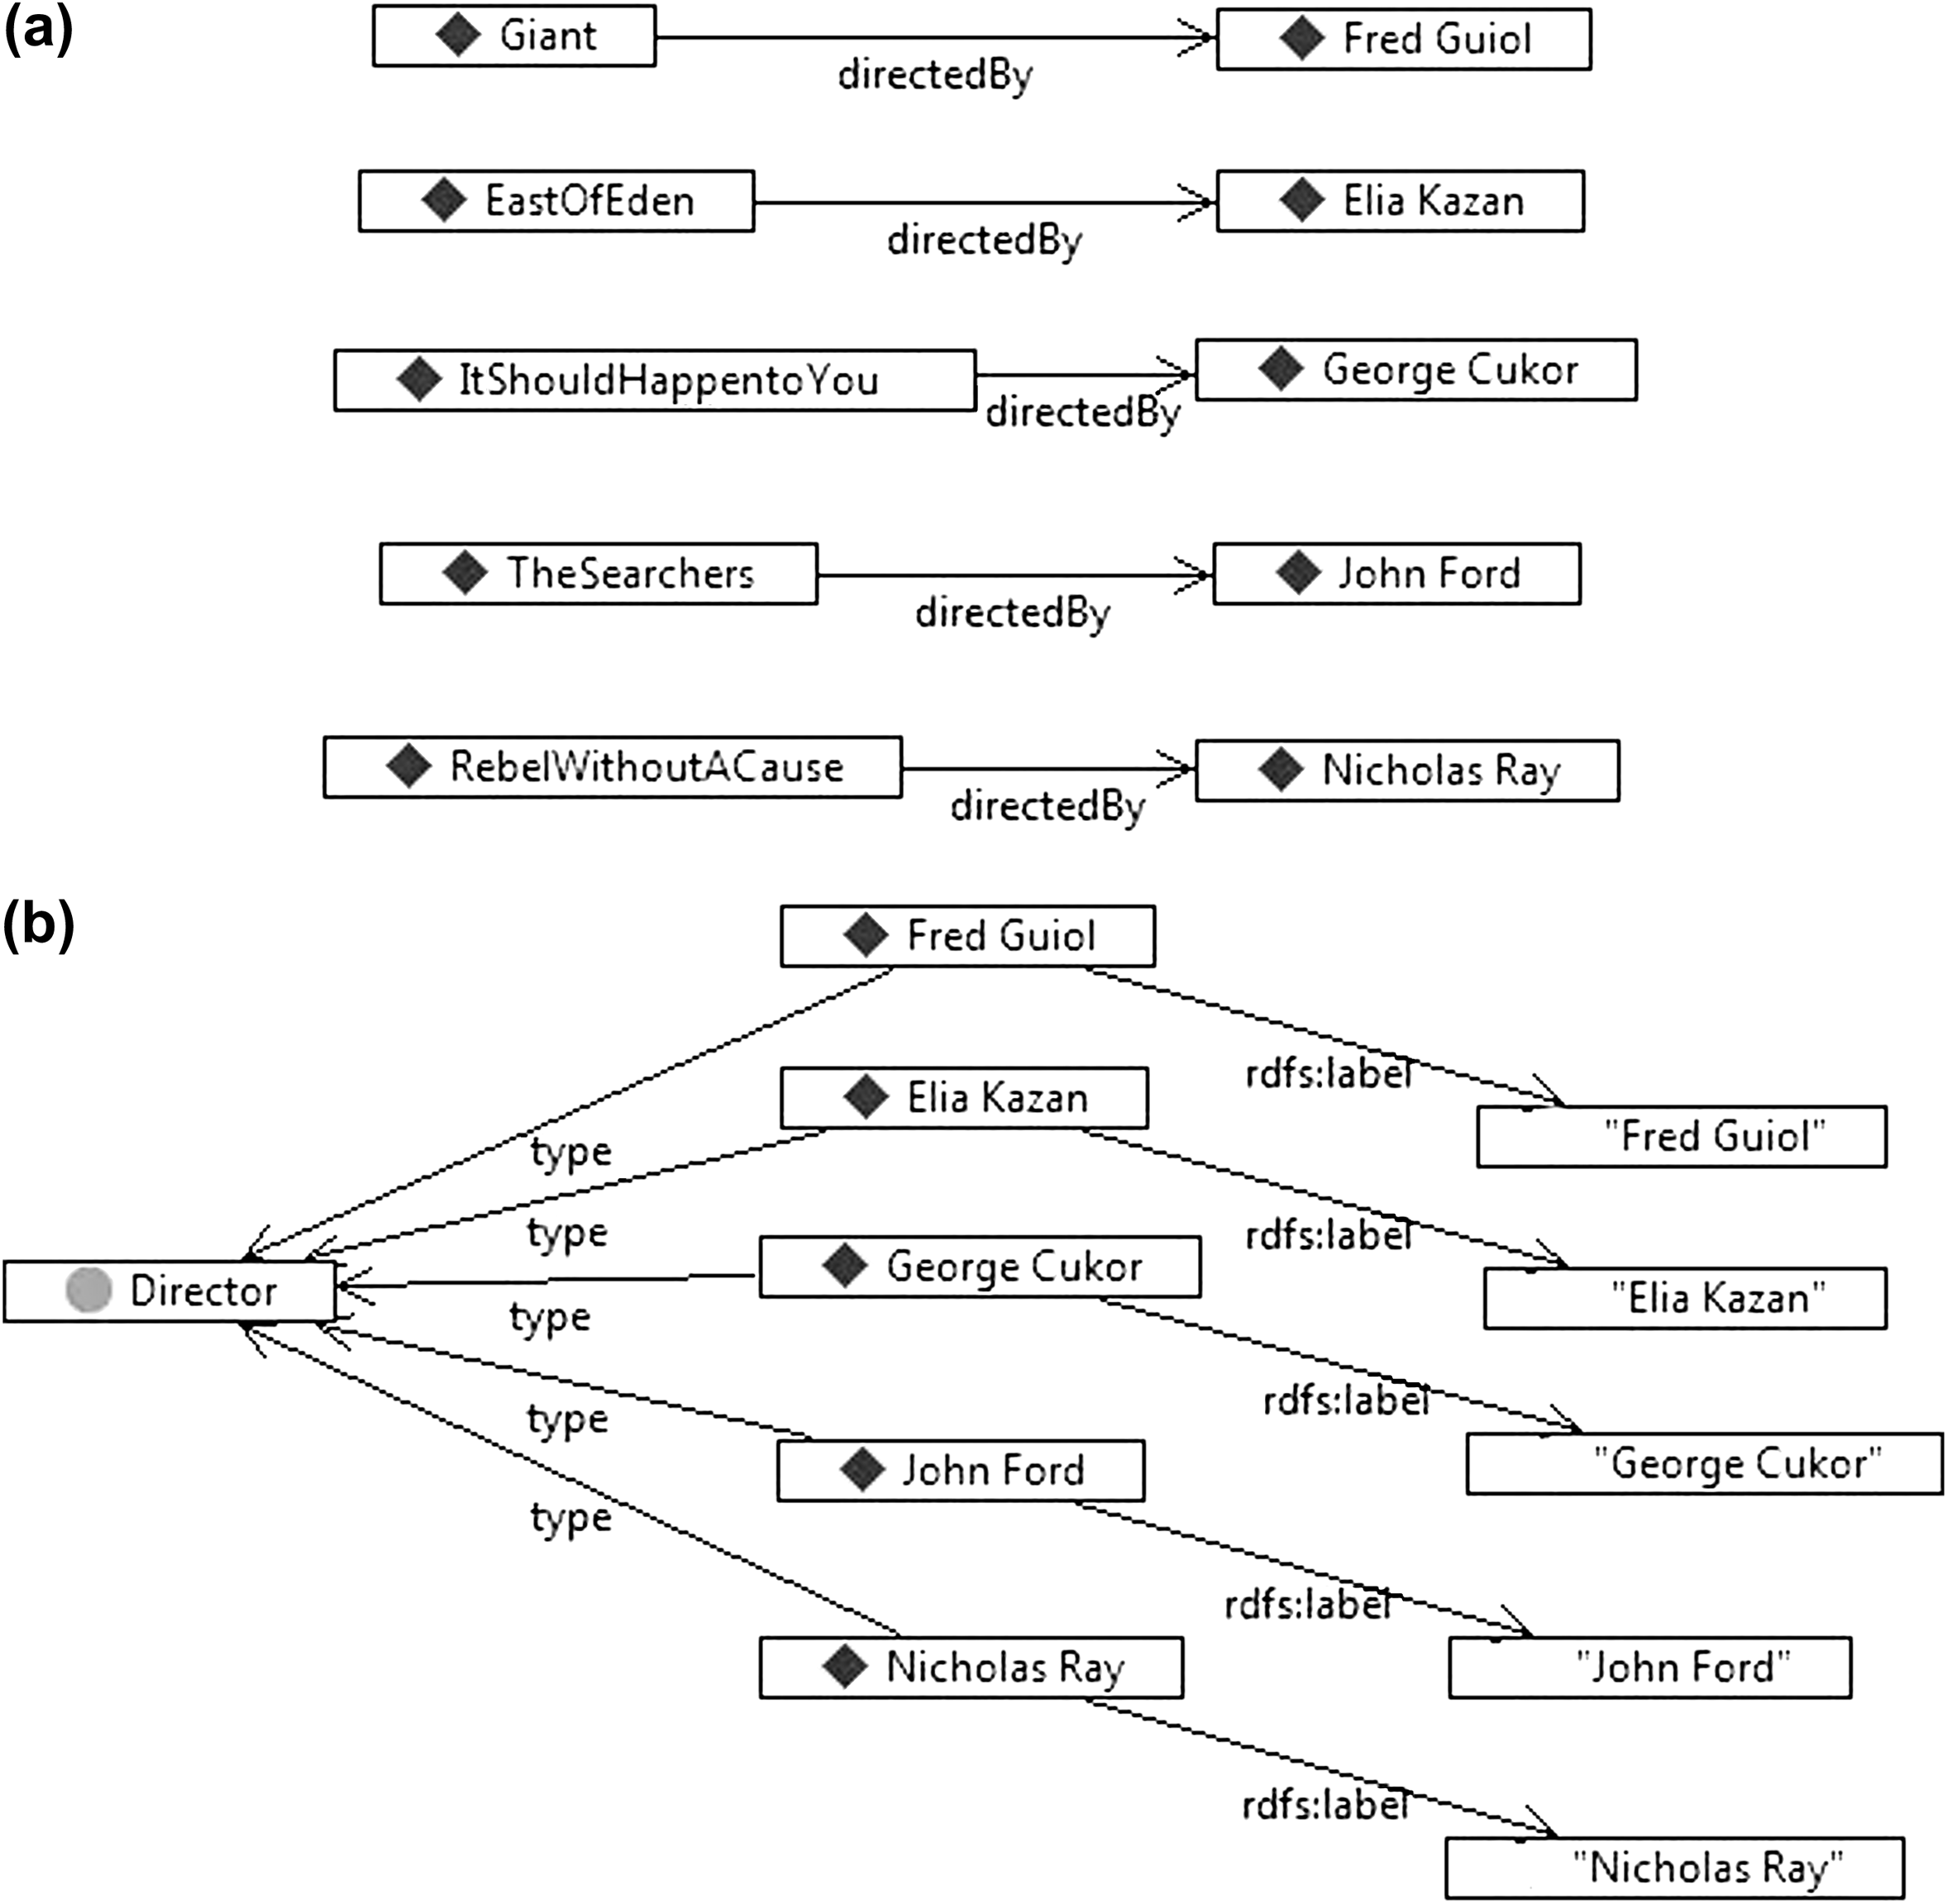
\includegraphics[width=5in]{media/f06-08.png}
\label{fig:ch6.8}
\caption{Constructing a model about directors from a query about movies.}
\end{figure}

some data set with a SPARQL endpoint -- that is, providing a service
that responds to the SPARQL 
protocol, providing access to that data set.

\section{SPARQL Rules -- Using SPARQL as a Rule Language}

SPARQL CONSTRUCT allows us to specify templates of new information based
on patterns found in old information. A specification of this sort is
sometimes called a Rule, since it provides a way to specify things like
``Whenever you see this, conclude that.'' Examples of rules include data
completeness rules (``If John's father is Joe, then Joe's son is
John''), logical rules (``If Socrates is a man, and all men are mortal,
then Socrates is mortal''), definitions (``If Ted's sister is Maria's
mother, then Ted is Maria's uncle''), as well as business rules
(``Customers who have done more than \$5000
worth of business with us are preferred customers''). Useful rules can
often be expressed simply in 
SPARQL -- though there are some subtleties.

Consider the following data:

\begin{lstlisting}
:John a :Man.
:Joe a :Man.
:Eunice a :Woman .
:Maria a :Woman .
:Caroline a :Woman .
:Ted a :Man .
:Socrates a :Man .
:Caroline :hasFather :John .
:Ted :hasBrother :John .
:John :hasFather :Joe .
:Maria :hasMother :Eunice .
:Maria :hasFather :Sargent .
:Ted :hasSister :Eunice .
\end{lstlisting}

We could write a rule relating father to son as

\begin{lstlisting}
CONSTRUCT { ?q1 :hasSon :q2 . }
WHERE { ?q2 :hasFather ?q1 }
\end{lstlisting}

But this wouldn't quite work the way we want; while we do construct

\begin{lstlisting}
:Joe :hasSon :John .
\end{lstlisting}

as desired, we also conclude

\begin{lstlisting}
:Sargent :hasSon :Maria .
\end{lstlisting}

which is not the usual interpretation of ``son''.

So, we need to restrict the rule a bit, so that it only applies to men:

\begin{lstlisting}
CONSTRUCT ?q1 :hasSon :q2 .
WHERE { ?q2 a :Man .
        ?q2 :hasFather ?q1 }
\end{lstlisting} 


SPARQL allows us to be as specific as we want when writing a rule. The
rule about Socrates is already restricted just to men:

\begin{lstlisting}
CONSTRUCT { ?q1 a :Mortal }
WHERE { ?q1 a :Man }
\end{lstlisting}

So we will conclude that Socrates (as well as Ted, John, Joe, and
Sargent) are mortal. But Maria and 
Eunice are off the hook -- we'll draw no conclusion about them.

The definition of ``uncle'' is easy to do in SPARQL

\begin{lstlisting}
CONSTRUCT { ?q1 :hasUncle ?q2 }
WHERE { ?q2 :hasSister ?s .
        ?q1 :hasMother ?s . }
\end{lstlisting}

This works fine to conclude that

\begin{lstlisting}
:Maria :hasUncle :Ted 
\end{lstlisting}

Since

\begin{lstlisting}
:Ted :hasSister :Eunice .
:Maria :hasMother :Eunice .
\end{lstlisting}

are both in the dataset. 

But this is both too permissive and too restrictive; for example, we
won't conclude that

\begin{lstlisting}
:Caroline :hasUncle :Ted .
\end{lstlisting}

despite the fact that this is true, and follows from the data and the usual understanding of family relationships.


One way to deal with this would be to write a system of rules -- some
dealing with completeness of concepts like mother, father, sister, and
brother, and another for uncle:

\begin{lstlisting}
CONSTRUCT {?q1 :hasSibling ?q2 } WHERE {?q1 :hasBrother ?q2 }
CONSTRUCT {?q1 :hasSibling ?q2 } WHERE {?q1 :hasSister ?q2 }
CONSTRUCT {?q1 :hasParent ?q2 } WHERE {?q1 :hasFather ?q2 }
CONSTRUCT {?q1 :hasParent ?q2 WHERE {?q1 :hasMother ?q2 }
\end{lstlisting}

Now we can define uncle in terms of siblings and parents:

\begin{lstlisting}
CONSTRUCT { ?q1 :hasUncle ?q2 }
WHERE { ?q2 :hasSibling ?parent .
        ?q2 a :Man .
        ?q1 :hasParent ?parent }
\end{lstlisting}


and can conclude both relationships:

\begin{lstlisting}
:Caroline :hasUncle :Ted .
:Maria :hasUncle :Ted .
\end{lstlisting}

(A complete model of family relationships will include quite a few data
completeness rules about siblings and parents. In Chapter~\ref{ch8}, we'll see a
more systematic way to organize a set of rules about these things.)

If we know how much business a customer has done with us, we can write a
business rule in 
SPARQL to sort out our preferred customers.

\begin{lstlisting}
:ACME :totalBusiness 5253.00 .
:PRIME :totalBusiness 12453.00 .
:ABC :totalbusiness 1545.00 .
\end{lstlisting}

The query

\begin{lstlisting}
CONSTRUCT { ?c a :PreferredCustomer }
WHERE {?c :totalBusiness ?tb .
       FILTER (?tb > 5000)  }
\end{lstlisting}

will assert all the preferred customers:

\begin{lstlisting}
:ACME a :PreferredCustomer .
:PRIME a :PreferredCustomer .
\end{lstlisting}

Later in this section, we'll see how to use aggregators and subqueries
to compute things like total business from information about various
business transactions.

For many of these queries, it was important to restrict the application
of the query to particular sets of individuals -- e.g., Uncles and Sons
can only be Men. This is a typical sort of restriction -- a rule only
applies to a particular class of things. In Chapter 7, we'll revisit
SPARQL rules, and see how an RDFS class structure can be used to
organize a set of interacting SPARQL rules.


\begin{challenge}
\textbf{USING SPARL TO TRANSFORM HIERARCHICAL DATA}
\label{chal:2}


In the data wilderness, information comes in many forms. Some of the
variety stems from all the systems and syntaxes that we use to represent
data -- spreadsheets, XML, relational databases, and even text
documents. RDF, as a general way to represent data, resolves many of the
more superficial issues with different data formats. But even within a
single system, there are a variety of ways to represent the same
information. If we want to deal with data from the wilderness, we often
have to transform data to make it easier to use.

We'll start with a simple example. Taking some of the family tree data
from the previous example (plus a few more):

\begin{lstlisting}
:Caroline :hasFather :John .
:John :hasFather :Joe .
:Eunice :hasFather :Joe .
:Maria :hasMother :Eunice .
:Maria :hasFather :Sargent .
:Joe :hasSon :Robert .
:Joe :hasSon :Ted .
:Ted :hasSon :Patrick .
\end{lstlisting}

We could speculate about how a dataset could get to be in such an
inconsistent state -- with some family relationships relating children
to their parents, while others relate parents to their children. The
data might originally come from multiple sources or have been entered
using multiple systems or by people following different methodologies.
But regardless of how it happened, this is a typical state of affairs in
the data wilderness; the data you find are organized in an inconsistent
way.

Now suppose we are interested in building a family tree that looks
something like Figure\ref{fig:ch6.9}, in which we see children and grandchildren,
regardless of gender, all in a single display. The tree is defined in a
uniform way -- Eunice has parent Joe, Maria has parent Eunice (and
Sargent), Caroline has parent John, etc.

\begin{figure}
\centering
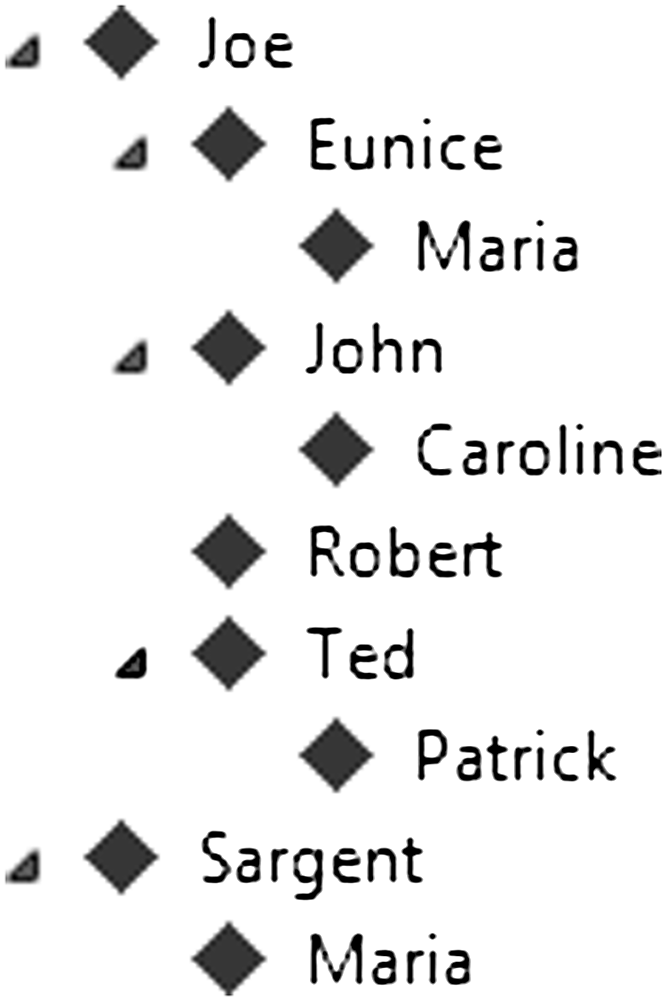
\includegraphics[width=5in]{media/f06-09.png}
\label{fig:ch6.9}
\caption{Family tree shown in a uniform manner.}
\end{figure}

All this information is available in the data set, if you abstract away
from gender words (like Son, Daughter, Mother, and Father) and re-order
some triples (turning hasSon around to be hasParent). How can we do this
using SPARQL?

We can do this by specifying a few rules as SPARQL constructs to map
these things into the form we want.

\begin{lstlisting}
CONSTRUCT {?s :hasParent ?o} WHERE {?s :hasMother ?o} 
CONSTRUCT {?s :hasParent ?o} WHERE {?s :hasFather ?o} 
CONSTRUCT {?s :hasParent ?o} WHERE {?o :hasSon ?s} 
CONSTRUCT {?s :hasParent ?o} WHERE {?o :hasDaughter ?s}
\end{lstlisting}

These queries match all the various forms of hasSon, hasDaughter,
hasMother, and hasFather and map them all into appropriate triples using
hasParent. The resulting triples are

\begin{lstlisting}
:Caroline :hasParent :John .
:Eunice :hasParent :Joe .
:John :hasParent :Joe .
:Maria :hasParent :Sargent .
:Maria :hasParent :Eunice .
:Patrick :hasParent :Ted .
:Robert :hasParent :Joe .
:Ted :hasParent :Joe .
\end{lstlisting}

These provide a uniform representation of the family tree and are
amenable for producing a display like that in 
Figure\ref{fig:ch6.9}.

We can extend this example to compute the gender of the family members,
by adding another triple to each query:

\begin{lstlisting}
CONSTRUCT {?s :hasParent ?o .
           ?o a :Woman .}
WHERE {?s :hasMother ?o} 
CONSTRUCT {?s :hasParent ?o.
           ?o a :Man .} 
WHERE {?s :hasFather ?o} 
CONSTRUCT {?s :hasParent ?o .
           ?s a :Man .} 
WHERE {?o :hasSon ?s} 
CONSTRUCT {?s :hasParent ?o .
           ?s a :Woman .}
WHERE {?o :hasDaughter ?s}
\end{lstlisting}
\end{challenge}

\section{Transitive queries (SPARQL 1.1)}

Hierarchical data can pose very particular problems when it comes to
querying. We can see this using the example of the family tree in Figure
5.9. Suppose we want to query for all members of Joe's family. We can
query for his children with a simple graph pattern:

\textbf{\textbf{Ask:}}

\begin{lstlisting}
SELECT ?member
WHERE { ?member :hasParent :Joe }
\end{lstlisting}

\textbf{\textbf{Answer:}}

\begin{tabular}{|l|}
\hline
?member\\
\hline
Eunice\\
John\\
Robert\\
Ted\\
\hline
\end{tabular}

If we want his grandchildren, we can build a slightly more complicated
query:

\textbf{\textbf{Ask:}}

\begin{lstlisting}
SELECT ?member
WHERE {?int :hasParent :Joe .
       ?member :hasParent ?int . }
\end{lstlisting}

\textbf{\textbf{Answer:}}

\begin{tabular}{|l|}
\hline
?member\\
\hline
Maria\\
Caroline\\
Patrick\\
\hline
\end{tabular}

If we wanted Joe's great-grandchildren, we could make another query, and
so on. But what if we want all of his family, regardless of how many
generations intervene? SPARQL 1.1 includes a transitivity operator for
just this purpose. If we include a ``*'' after a property name, then the
triple matches any number of chained occurrences of the same property.

\textbf{\textbf{Ask:}}

\begin{lstlisting}
SELECT ?member
WHERE {?member :hasParent* :Joe . }
\end{lstlisting}

\textbf{\textbf{Answer:}}

\begin{tabular}{|l|}
\hline
?member\\
\hline
Joe\\
Eunice\\
Maria\\
John\\
Caroline\\
Robert\\
Ted\\
\\
Patrick\\
\hline
\end{tabular}


Notice that Joe himself is matched -- even chains of zero triples will
match. If we want to insist that there is at least one triple in the
chain (Joe's progeny, not including himself), we can use a + instead:

\textbf{\textbf{Ask:}}

\begin{lstlisting}
SELECT ?member
WHERE {?member :hasParent+ :Joe . }
\end{lstlisting}

\textbf{\textbf{Answer:}}

\begin{tabular}{|l|}
\hline
?member\\
\hline
Eunice\\
Maria\\
John\\
Caroline\\
Robert\\
Ted\\
\\
Patrick\\
\hline
\end{tabular}

(SPARQL 1.1 includes a number of variations on this theme, beyond what
we cover here. Details can be found in the SPARQL 1.1 standard.)

\begin{challenge} 
\textbf{USING SPARQL TO RECORD SAMENESS IN THE LINKED MDB}
\label{chal:3}

When merging information from multiple sources, it is typical for the
same entity to appear in each data source with a different identifier.
Even in the case of a single data source, it is not unusual for the same
item to appear multiple times, with a different identifier each time.
This is especially common when the data source is implemented as a
relational database, where common practice involves separating out
information based on the role an entity plays in an application.

The Linked Movie DataBase\footnote{http://linkedmdb.org/} (LinkedMDB) is an open data source containing
data about movies. The LinkedMDB is based on a relational database
containing information about movies, actors, directors, etc. The
underlying database includes information about what movies directors
made as well as what movies actors played in. This information is
represented in two separate tables -- a director table and an actor
table. When converted to triples, this database structure results in two
classes in the published SPARQL endpoint with corresponding names --
director and actor.

Members of the classes in the linkedMDB are given numeric URIs -- here
is a very small excerpt of data from that endpoint:

\begin{lstlisting}
actor:29753
     rdf:type linkedmdb:actor ;
     linkedmdb:actor_name "Clint Eastwood" .

film:38599
     rdf:type linkedmdb:film ; 
     dc:title "Unforgiven" ; 
     linkedmdb:actor actor:29753 ; 
     linkedmdb:director director:8533 .

director:8533
     rdf:type linkedmdb:director ;
     linkedmdb:director_name "Clint Eastwood" .
\end{lstlisting}

In this fragment, there is a movie whose \texttt{dc:title} is ``Unforgiven'' (the
namespace dc stands for ``Dublin Core,'' a metadata standard used by
many libraries worldwide that includes standard terms for titles,
authors, publication dates, etc.), stars an actor (number 29753) whose
name is ``Clint Eastwood,'' and was directed by a director (number 8533)
whose name is ``Clint Eastwood.'' Is the fact that both of these people
are named ``Clint Eastwood'' enough for us to conclude that they are the
same person?

Fortunately, there is another triple for each of these resources in the
LinkedMBD dataset:

\begin{lstlisting}
actor:29753 foaf:page freebase:9202a8c04000641f8000000000056de6 .
director:8533 foaf:page freebase:9202a8c04000641f8000000000056de6 .
\end{lstlisting}

Freebase was a linked data resource that (among other things) provided an
identity service for resources on the Web. Even though no new items are being added to Freebase
(it has been absorbed into a larger Google knowledge graph), Freebase references still provide unique
identifiers for many resources on the web. 
Any data source on the Web
can refer to a freebase URI, to unambiguously identify its own
resources. Freebase is not the only such service -- in the life
sciences, there are several such identification services for proteins,
genes, and other biological entities, and others exist for a number of
areas.  For more general use, dbpedia is a de-facto source of unique identifiers for anything that
is mentioned in wikipedia. 

In this case, we can use this information to determine that these two
people named ``Clint Eastwood'' are in fact the same person; since
linkedMDB links both of them to the same Freebase resource, they must be
the same. But what can we do with that information?

We can use SPARQL to detect identities of this sort and record it as a
new triple.

\begin{lstlisting}
CONSTRUCT {?a skos:exactMatch ?b }
WHERE {?a foaf:page ?page .
       ?b foaf:page ?page . }
\end{lstlisting}

You can understand this query, even without knowing anything else about
the resources in it -- \texttt{foaf:page} and \texttt{skos:exactMatch} (though these will
be discussed in Chapters~\ref{ch9} and \ref{ch10}). This query simply says that any two
resources with the same \texttt{foaf:page} are \texttt{skos:exactMatch} to one another. On
this data set, we get the following triples:

\begin{lstlisting}
actor:29753 skos:exactMatch director:8533 . 
director:8533 skos:exactMatch actor:29753 . 
director:8533 skos:exactMatch director:8533 . 
actor:29753 skos:exactMatch actor:29753 .
\end{lstlisting}

These triples indeed encode the identity match that we observed -- that
the director of \emph{Unforgiven} also played in it. But it brings along
some extra baggage -- the exactMatch appears twice, once relating the
actor to the director, and another time relating the director to the
actor. Furthermore, we have two rather trivial results, that every actor
is an exact match to itself (and the same for directors). These extra
results appear because SPARQL finds every match for the graph pattern in
the data; and all four assignments of \texttt{?a} and \texttt{?b} to director:8533 and
actor:29753 satisfy the pattern (they have the same values for \texttt{:page}).
These extra triples don't really cause any harm -- after all, it seems
correct to say that something is an exact match to itself -- but at the
same time, they are somewhat superfluous. In an earlier example, we were
able to drop duplicates by using the DISTINCT keyword in SPARQL. In this
case, we need something else, because  all four of these triples are
already distinct (i.e., no two have the same value for all three
positions; subject, predicate and object).

We can use a FILTER clause to eliminate many of these spurious values --
since we aren't interested in statements that say that an actor is an
exact match for himself, we can eliminate these with a filter for
matching the same values:

\begin{lstlisting}
CONSTRUCT { ?a skos:exactMatch ?b }
WHERE { ?a foaf:page ?page . 
        ?b foaf:page ?page .
        FILTER (?a != ?b) }
\end{lstlisting}

The comparison != in a filter stands for ``not equal'' -- it evaluates
to `true' just if \texttt{?a} and \texttt{?b} are not the same. This results in the
following triples:

\begin{lstlisting}
actor:29753 skos:exactMatch director:8533 . 
director:8533 skos:exactMatch actor:29753 .
\end{lstlisting}

This is an improvement. And if we didn't know that \texttt{skos:exactMatch} is a
symmetric property (see Chapter~\ref{ch11}), we would be satisfied at this point that we had filtered out all
the spurious triples.

If we want to go one step further, we can sort these triples so that
only the first one in each pair is kept. The FILTER clause in SPARQL
includes capabilities for managing data types borrowed from XML, so
there are many ways to compare values. We can convert a URI to an XML,
then compare the strings. We can use this trick to reduce our results to
a single triple:

\begin{lstlisting}
CONSTRUCT {?a skos:exactMatch ?b }
WHERE {?a foaf:page ?page .
       ?b foaf:page ?page .
       FILTER (xsd:string (?a) >  xsd:string (?b)) }
\end{lstlisting}


This query will keep a triple only when the subject comes after the
object in alphabetical order; this means that of the two triples in the
previous result, only the second one is kept:

\begin{lstlisting}
director:8533 skos:exactMatch actor:29753 .
\end{lstlisting}

In general, there could be many ways to determine that two resources are
actually referring to the same thing; having a reference system like
Freebase or dbpedia is the easiest way. The need for such reference systems of this
kind did not begin with the Semantic Web -- it has been around for
centuries. The Semantic Web simply provides a means for publishing these
systems, and referring to them, on the Web. When there isn't a reference
system like Freebase around, more complex means of identifying
individuals can be used. The same strategy using SPARQL CONSTRUCT can be
used to determine these matches and to record them using
\texttt{skos:exactMatch}. For example, suppose that the data set included
information about date and place of birth. If it is reasonable to assume
in the dataset that two people who share the same name, place, and date
of birth are indeed the same persons, then the query

\begin{lstlisting}
CONSTRUCT {?a skos:exactMatch ?b }
WHERE {?a :name ?name ;
          :birthplace ?bplace ;
          :birthdate ?date .
       ?b :name ?name ;
          :birthplace ?bplace ;
          :birthdate ?date .
       FILTER (xsd:string (?a) >  xsd:string (?b)) }
\end{lstlisting}

will construct triples asserting the matches between these resources.

The Semantic Web doesn't provide any particular mechanism for
determining that one resource refers to the same individual as another;
it provides a means for writing down such a conclusion and publishing it
on the Web.

Now that we know that both people named Clint Eastwood are really the
same person, we are in a position to answer the question, ``Which
directors played in movies they directed?'' We can answer it with the
following query:

\textbf{\textbf{Ask:}}
\begin{lstlisting}
SELECT ?director
WHERE { ?dir foaf:made ?m ;
             linkedmdb:director_name ?director ;
             skos:exactMatch ?player . 
        ?m linkedmdb:actor ?player .
       }
\end{lstlisting}

\textbf{\textbf{Answer:}}

\begin{tabular}{|l|}
\hline
?director\\
\hline
``Clint Eastwood''\\
\hline
\end{tabular}
\end{challenge}

\begin{challenge}
\textbf{USING SPARQL TO COPY AN EXCERPT OF A DATABASE}
\label{chal:4}

An RDF data set is often made up of a very large number of triples.
There are a number of reasons why one might want to create a smaller
excerpt of such a data set:

\begin{enumerate}
\item  The data set might be available only as a network resource, with
inconsistent connectivity. You might want to keep a more robust copy of
the information that is used the most.

\item  The data set might be very large, resulting in slow query time for
complex queries. You might want to keep a cache of a small, relevant
part of the database for fast queries.

\item  The data set might contain sensitive information that should not be
disclosed to certain audiences. You might want to make a copy of the less sensitive information for public access.
\end{enumerate}


In any case, it can be useful to be able to select a part of a data set
for separate storage. This can be done with
SPARQL CONSTRUCT queries.

Following on the previous example, suppose we wanted to create a data
set that contains information about the film \emph{Unforgiven}. We want
to include the actors who played in it, its director, producer, and any
other information about it.

In the LinkedMDB, Unforgiven is given the resource name film:38599. How
can we select all the information in the LinkedMDB about Unforgiven?

Depending on just what we mean by ``all'' the information, we can start
with a simple query:

\begin{lstlisting}
CONSTRUCT {film:38599 ?p ?o . } WHERE {film:38599 ?p ?o . }
\end{lstlisting}

This apparently trivial query selects all the triples from the data set
with film:38599 as the subject. From the full LinkedMDB, it returns a
few dozen results, including the triples:

\begin{lstlisting}
film:38599 rdf:type linkedmdb:film . 
film:38599 dc:title "Unforgiven" .
film:38599 linkedmdb:actor actor:29753 . 
film:38599 linkedmdb:actor actor:30285 .
film:38599 linkedmdb:director director:8533 . 
film:38599 linkedmdb:editor editor:2920 .
\end{lstlisting}

This is a good start for getting ``all'' the information about
Unforgiven. It includes the information about actors and directors we
need to figure out that it is one of the movies that Clint Eastwood both
directed and starred in. But there could be more information in the data
set that is relevant to this movie -- for instance, there is the triple

\begin{lstlisting}
director:8522 foaf:made film:38599 .
\end{lstlisting}

This triple doesn't appear in the results of the query, since in this
case, film:38599 is the object of the triple, not the subject. We can
use a very similar query to fetch these triples:

\begin{lstlisting}
CONSTRUCT {?s ?p film:38599. } WHERE {?s ?p film:38599 . }
\end{lstlisting}

This will fetch all the triples in which \emph{Unforgiven} appears as
the object, including the \texttt{foaf:made} triple above. This is a more
comprehensive notion of what it could mean to fetch ``all'' the
information about a particular resource.

But even these triples might not seem like quite enough to tell us all
about \emph{Unforgiven}; for example, who is actor:30285? In addition to
the information about the movie itself, we might want to also identify
information about related entities. A more elaborate graph pattern can
do this as well:

\begin{lstlisting}
CONSTRUCT { ?s ?p ?o }
WHERE { film:38599 ?p1 ?s . }
        ?s ?p ?o . }
\end{lstlisting}

The pattern

\begin{lstlisting}
?s ?p ?o
\end{lstlisting}

matches every triple in the data set, subject to the bindings so far. In
this case, \texttt{?s} is already bound from the first triple pattern to anything
that is related (in any way) to Unforgiven. So, in this case, this
pattern copies all triples whose subjects are related to Unforgiven.

For example, since

\begin{lstlisting}
film:38599 linkedmdb:actor actor:30285 .
\end{lstlisting}

is in the data set, this query will find all the triples starting with
actor:30285, including

\begin{lstlisting}
actor:30285 linkedmdb:actor_name "Richard Harris" .
\end{lstlisting}

If we merge together the results of all of these queries, we can create
a comprehensive cache of all information regarding Unforgiven. This
method was used to create most of the sample files for the examples in
this chapter.
\end{challenge}

\section{Advanced Features of SPARQL}

\subsection{Limits and ordering}

Suppose we want to know the movies that James Dean played in, and the
dates they were released:

\textbf{\textbf{Ask:}}

\begin{lstlisting}
SELECT ?movie ?date
WHERE { :JamesDean :playedIn ?m.
        ?m rdfs:label ?movie .
        ?m dc:date ?date . }
\end{lstlisting}


\textbf{\textbf{Answer:}}

\begin{tabular}{|ll|}
\hline
?movie&?date\\
\hline
Giant&1956\\
EastOfEden&1955\\
RebelWithoutaCause&1955\\
\hline
\end{tabular}

These answers come back in no particular order; different SPARQL
implementations (and even the same implementation, at different times)
are free to produce the results in any order they like.

We can specify an ordering in the query for the results using the
directive ORDER BY. The ORDER BY directive comes after the graph pattern
and specifies one or more variables to use to determine the order in
which the results are returned. The following two examples show how this
works, ordering by 
?date and \texttt{?movie} (title), respectively:

\textbf{\textbf{Ask:}}

\begin{lstlisting}
SELECT ?title ?date
WHERE { :JamesDean :playedIn ?movie.
        ?movie rdfs:label ?title .
        ?movie dc:date ?date . }
ORDER BY ?date
\end{lstlisting}

\textbf{\textbf{Answer:}}

\begin{tabular}{|ll|}
\hline
?title&?date\\
\hline
EastOfEden&1955\\
RebelWithoutaCause&1955\\
Giant&1956\\
\hline
\end{tabular}

\textbf{\textbf{Ask:}}

\begin{lstlisting}
SELECT ?title ?date
WHERE { :JamesDean :playedIn ?movie.
        ?movie rdfs:label ?title .
        ?movie dc:date ?date . }
ORDER BY ?title
\end{lstlisting}

\textbf{\textbf{Answer:}}

\begin{tabular}{|ll|}
\hline
?title&?date\\
\hline
EastOfEden&1955\\
Giant&1956\\
RebelWithoutaCause&1955\\
\hline
\end{tabular}

(Note that SPARQL uses simple notions of ordering for each type of
value: numbers in numerical order, strings in alphabetic order, etc.)

Sometimes we don't want all the possible matches to a query -- for a
user interface, we might want to limit the number of items we display at
a time. Or we might want to provide a report of just the highest values
-- the ``top ten'' results. To accommodate these sorts of requests,
SPARQL includes a LIMIT directive, with which the query can specify the
maximum number of results to be fetched. LIMIT works together with ORDER
BY to determine which items to return; when LIMIT is used without ORDER
BY, the SPARQL implementation is free to fetch any matching results, up
to the specified limit.

So to find the earliest James Dean movie, we can ORDER BY ?date and
specify a LIMIT of 1:

\textbf{\textbf{Ask:}}

\begin{lstlisting}
SELECT ?title
WHERE { :JamesDean :playedIn ?m.
        ?m rdfs:label ?title .
        ?m dc:date ?date . 
ORDER BY ?date
LIMIT 1
\end{lstlisting}

\textbf{\textbf{Answer:}}

\begin{tabular}{|l|}
\hline
?title\\
\hline
East Of Eden\\
\hline
\end{tabular}

All three stars (James Dean, Natalie Wood, and Sal Mineo) of \emph{Rebel
without a Cause} died young under tragic circumstances. Which one died
first?

\textbf{\textbf{Ask:}}

\begin{lstlisting}
SELECT ?first
WHERE { ?who :playedIn :RebelWithoutaCause .
        ?who rdfs:label ?first .
        ?who :diedOn ?date
ORDER BY ?date
LIMIT 1
\end{lstlisting}


\textbf{\textbf{Answer:}}

\begin{tabular}{|l|}
\hline
?first\\
\hline
James Dean\\
\hline
\end{tabular}

By default, SPARQL orders results in ascending order. We can reverse the
ordering, and find the star who lived the longest with the keyword DESC
(for ``descending'')

\textbf{\textbf{Ask:}}

\begin{lstlisting}
SELECT ?last
WHERE { ?who :playedIn :RebelWithoutaCause ;
             rdfs:label ?last ;
             :diedOn ?date .
ORDER BY DESC (?date)
LIMIT 1
\end{lstlisting}

\textbf{\textbf{Answer:}}

\begin{tabular}{|l|}
\hline
?last\\
\hline
Sal Mineo\\
\hline
\end{tabular}

\subsection{AGGREGATES AND GROUPING (SPARQL 1.1)}

SPARQL 1.1 includes a facility for specifying aggregate functions of
data. Specifically, it provides aggregate functions COUNT, MIN, MAX,
AVG, and SUM. These aggregates can be used alongside any graph pattern,
computing a result for all matches for the pattern.

For example, we could find out how many movies James Dean has played in:

\begin{lstlisting}
SELECT (COUNT (?movie) AS ?howmany)
WHERE { :JamesDean ?playedIn ?movie . }
\end{lstlisting}


The syntax of SPARQL aggregates appears in the SELECT clause -- the
aggregate expression appears in parentheses, starting with the aggregate
word, followed by the variable to be aggregated (also in parentheses),
then the keyword AS followed by a new variable, which will be bound to
the aggregated value. In this case, the query result is a single binding
for \texttt{?howmany}

\begin{tabular}{|l|}
\hline
?howmany\\
\hline
3\\
\hline
\end{tabular}

Sums work in much the same way -- suppose we want to add up the amount
of business we have done each year with various customers, and we have
data about our sales -- which company made the purchase, the amount of
the purchase, and the year in which the purchase was made. The data are
shown in tabular form here:


\begin{tabular}{|lll|}
\hline
Company&Amount&Year\\
\hline
ACME&\$1250&2010\\
PRIME&\$3000&2009\\
ABC&\$2500&2009\\
ABC&\$2800&2010\\
PRIME&\$1950&2010\\
ACME&\$2500&2009\\
ACME&\$3100&2010\\
ABC&\$1500&2009\\
ACME&\$1250&2009\\
PRIME&\$2350&2009\\
PRIME&\$1850&2010\\
\hline
\end{tabular}


As triples, each row is represented as four triples, with an arbitrary
URI for the row. Each row is a member of a single class, \texttt{:Sale}. So the
first row looks like the triples:

\begin{lstlisting}
:row1 a :Sale ;
      :company :ACME ;
      :amount 1250 ;
      :year 2010 .
\end{lstlisting}

Using this representation in triples, we can find our total sales using
a SUM aggregator:

\textbf{\textbf{Ask:}}

\begin{lstlisting}
SELECT (SUM (?val) AS ?total)
WHERE {?s a :Sale ;
          :amount ?val  }
\end{lstlisting}

\textbf{\textbf{Answer:}}

\begin{tabular}{|l|}
\hline
?total\\
\hline
24050.00\\
\hline
\end{tabular}

With this sort of data, we are interested in breaking this answer down
in various ways; how much business did we do with each customer? How
much business did we do in a given year? SPARQL allows us to organize
the query in these ways, using the notion of GROUP BY. For instance, we
can find the amount of business for each year by grouping by years:

\textbf{\textbf{Ask:}}

\begin{lstlisting}
SELECT ?year (SUM (?val) AS ?total)
WHERE { ?s a :Sale ;
           :amount ?val ;
           :year ?year  }
GROUP BY ?year
\end{lstlisting}

\textbf{\textbf{Answer:}}

\begin{tabular}{|ll|}
\hline
?year&?total\\
\hline
2009&13100.00\\
2010&10950.00\\
\hline
\end{tabular}

The GROUP BY keyword comes after the graph pattern and informs the
aggregate how to group the sums; instead of summing all the results, it
sums results grouped by the specified variable. In this case, the sum is
grouped by \texttt{?year}. The GROUP BY variable must already have been bound in
the graph pattern; these values are used to sort the results for
aggregation. Since a variable mentioned in the GROUP BY clause will have
the same value for every summand for a particular sum, it is sensible to
include it in the SELECT clause (if desired). Other variables (like \texttt{?s}
and \texttt{?val}) will have different values for each summand, and hence won't
have a single defined value for a sum; these variables are not available
for inclusion in the SELECT clause.

We can sort by more than one variable at a time:

\textbf{\textbf{Ask:}}

\begin{lstlisting}
SELECT ?year ?company (SUM (?val) AS ?total)
WHERE { ?s a :Sale ;
           :amount ?val ;
           :year ?year ;
           :company ?company . }
GROUP BY ?year ?company
\end{lstlisting}

\textbf{\textbf{Answer:}}

\begin{tabular}{|lll|}
\hline
?year&?company&?total\\
\hline
2009&ACME&3750.00\\
2009&ABC&4000.00\\
2009&PRIME&5350.00\\
2010&ACME&4350.00\\
2010&PRIME&3800.00\\
2010&ABC&2800.00\\
\hline
\end{tabular}

This tells us how much business we did with each customer in a
particular year. If we'd like to find out customers that did more than
\$5000 of business in some year, we can show only some of these results,
using the keyword HAVING to choose particular results:

\textbf{\textbf{Ask:}}

\begin{lstlisting}
SELECT ?year ?company (SUM (?val) AS ?total)
WHERE { ?s a :Sale ;
           :amount ?val ;
           :year ?year ;
           :company ?company . }
GROUP BY ?year ?company
HAVING (?total  5000)
\end{lstlisting}

\textbf{\textbf{Answer:}}

\begin{tabular}{|lll|}
\hline
?year&?company&?total\\
\hline
2009&PRIME&5350.00\\
\hline
\end{tabular}

PRIME was the only customer who satisfied this criterion, which they did
in 2009. The keywords HAVING and FILTER are very similar; both of them
introduce a condition that is to be met by the results. FILTER refers to
variables bound within a particular graph pattern, hence the FILTER
keyword always appears in the pattern (between ``\{`` and ''\}''), while
HAVING refers to variables defined by aggregations in the SELECT clause,
and hence always appears outside a graph pattern.

\subsection{Subqueries (SPARQL 1.1)}

A subquery is a query within a query. Since a SPARQL graph pattern can
include arbitrary connections between variables and resource
identifiers, there isn't as much need to have subquery as there is in
other query languages. In fact, for basic SPARQL (i.e., without limit or
aggregate functions), there is no need for subquery at all.

But subqueries can be useful when combining limits and aggregates with
other graph patterns. A question has to be pretty complex to require a
subquery in SPARQL. A subquery limits the scope of things like
aggregators, orderings, and limits to just part of the query. Following
along the example using customer sales above, we notice that some
companies increased their sales from 2009 to 2010, while others
decreased. We can use subqueries to find out which ones increased their
sales during that time:

\textbf{\textbf{Ask:}}

\begin{lstlisting}
SELECT ?company
WHERE {
    {SELECT ?company ((SUM(?val)) AS ?total09)
     WHERE {
            ?s a :Sale ;
               :amount ?val ;
               :company ?company ;
               :year 2009 .  }
     GROUP BY ?company  . }
    {SELECT ?company ((SUM(?val)) AS ?total10)
     WHERE {
            ?s a :Sale ;
               :amount ?val ;
               :company ?company ;
               :year 2010 . }
     GROUP BY ?company  . }
    FILTER (?total10  ?total09) .
}
\end{lstlisting}
\textbf{\textbf{Answer:}}

\begin{tabular}{|l|}
\hline
?company\\
\hline
ACME\\
\hline
\end{tabular}

The two subqueries in this example compute the total sales for years
2009 and 2010, respectively. The FILTER retains only the matches in
which the 2010 total exceeds the 2009 totals -- customers who did more
business in 2010 than in 2009. Each subquery (including GROUP BY etc. at
the end) is enclosed in braces. Within the subqueries, variables have
their own scope; that is, the variable \texttt{?val} in each of these subqueries
matches completely different values (in one subquery, it matches the
2009 values; in the other, it matches the 2010 values). This sort of
computation requires subqueries, since it involves independent subsets
of the data to be compared.

Another application of subqueries is to bring the power of aggregates
(available only in SELECT queries) to other SPARQL query constructs
(like ASK and CONSTRUCT). Earlier, we saw a query that selected the
companies who had done more than \$5000 worth of business in a single
year.

Suppose we wanted to use this result as part of a CONSTRUCT query --
where would we put the aggregation specification? This can be handled
uniformly with a subquery, as in the following example:

\begin{lstlisting}
CONSTRUCT { ?company a :PreferredCustomer.
            ?company :totalSales ?total . }
WHERE {SELECT ?year ?company (SUM (?val) as ?total)
       WHERE { ?s a :Sale ;
                  :amount ?val ;
                  :year ?year ;
                  :company ?company . }
       GROUP BY ?year ?company 
       HAVING (?total  5000)
      }
\end{lstlisting}


This results in two triples:

\begin{lstlisting}
:PRIME a :PreferredCustomer . 
:PRIME :totalSales 5350.00 .
\end{lstlisting}


The subquery is the same query we saw before, determining which
companies did more than \$5000 of business in a single year. The
CONSTRUCT query creates a graph with just the information about
preferred customers -- their preferred status as membership in the class
\texttt{:PreferredCustomer}, and the total sales as a numeric value.

\subsection{UNION}

A graph pattern is made up of several triples -- all of which have to
match in order for the pattern to match. In logical terms, this means
that there is an implicit ``and'' operation between the triples. One
could correctly read a graph pattern as saying ``the first triple
matches AND the second triple matches AND the third triple matches .''
But there are times when we might want to say that this triple matches
OR that triple matches. For those times, SPARQL provides UNION.

UNION combines two graph patterns, resulting in the set union of all
bindings made by each pattern. Variables in each pattern take values
independently (just as they do in subqueries), but the results are
combined together.

A simple example would be to find out all the actors who played either
in \emph{Rebel without a Cause} or

\emph{Giant}. Each of these is a simple query; we can get all the
answers by making a UNION of the two queries:

\textbf{\textbf{Ask:}}

\begin{lstlisting}
SELECT ?actor
WHERE {
        {?actor :playedIn :Giant .}
        UNION
        {?actor :playedIn :RebelWithoutaCause . }
      }
\end{lstlisting}


\textbf{\textbf{Answer:}}

\begin{tabular}{|l|}
\hline
actor\\
\hline
Ann Doran\\
Carroll Baker\\
Elizabeth Taylor\\
James Dean\\
James Dean\\
Jim Backus\\
Mercedes McCambridge\\
Natalie Wood\\
Rock Hudson\\
Sal Mineo\\
Sal Mineo\\
\hline
\end{tabular}

Some names appear twice, if the actor appeared in both movies. This
repetition can be removed by using the DISTINCT keyword.

UNION can be used in the context of CONSTRUCT as well. In a challenge
earlier in this chapter, we used SPARQL to transform hierarchical
information, by mapping several related relationships (mother, father,
son, daughter) onto a single hierarchy (parent); the resulting triples
were shown in Figure\ref{fig:ch6.9}. This involved four CONSTRUCT queries, with an
implicit understanding that all the triples resulting from each query
would be merged. This is a perfectly fine assumption, if the queries are
run in the context of a program that indeed combines all the results
(e.g., by adding all the triples to the same triple store). But with
UNION, we can specify explicitly that the triples are to be combined. We
can take the graph pattern for each of the triples, and combine them all
with the UNION operator, thus:

\begin{lstlisting}
CONSTRUCT {?s :hasParent ?o}
WHERE{ {?s :hasMother ?o}
       UNION
       {?s :hasFather ?o}
       UNION
       {?o :hasSon ?s}
       UNION
       {?o :hasDaughter ?s}
     }
\end{lstlisting}

The result of this query is the same as the combined results of the
queries in the Challenge, i.e., the set of hasParent relationships shown
in Figure~\ref{fig:ch6.9}.

\subsection{ASSIGNMENTS (SPARQL 1.1)}

Suppose we want to query the full names of the authors of the book
``Semantic Web for the Working Ontologist.'' We can easily find first
names and last names, but how do we get the full names? It is a simple
enough computation -- concatenate the first and last names together,
with an embedded space. But the string ``James Hendler'' is nowhere to
be found in the data set. How do we create it?

Tell-and-ask systems typically answer questions based on information
that was told to them -- this is true for spreadsheets, notebooks,
databases, and RDF stores. But many tell-and-ask systems go
beyond this, and provide ways for you to specify information that you
didn't (directly) tell the system. We have already seen how this can be
done with aggregators in SPARQL -- the sums, averages, counts, etc., are
information that was not directly told to the system, but was computed
from information that was already there.

But sometimes we would like to specify a special purpose computation as
part of the ask process. Spreadsheets excel at this functionality, with
the ability for the user to specify arbitrary formulas that will be
calculated and updated whenever data are changed or entered. Databases
have stored procedures that execute arbitrary code based on information
in the database. SPARQL provides a similar capability through query-time
assignments. An assignment lets the query write specifically the value
of a variable through some computation -- ``assigning'' a value to that
variable, rather than matching some value in the data.

Assignments are not supported in the SPARQL 1.0 standard but are
supported in the 1.1 standard. Assignments are expressed with the
keyword BIND,  as follows:

\begin{lstlisting}
BIND ( expression (...) AS ?var)
\end{lstlisting}

The expression can include arithmetic formulas (using the usual
operators +. -. *, /, etc.) or a series of function calls, and references to other variables
that have already been matched or bound. Like stored
procedures in relational databases, the function calls can include
arbitrary programs in a variety of programming languages. For the
examples in this book, we will restrict ourselves to some standard
functions, those from the XPATH spec for XML.

Suppose we have some data about books and their authors, including the
following data:

\begin{lstlisting}
:DeanAllemang rdf:type :Person ;
              :firstName "Dean" ;
              :lastName "Allemang" .

:JimHendler rdf:type :Person ;
            :firstName "James" ;
            :lastName "Hendler" .

:FabienGandon rdf:type :Person ;
              :firstName "Fabien" ;
              :lastName "Gandon" .

:WorkingOntologist rdf:type :Book ;

rdfs:label "Semantic Web for the Working Ontologist" ;

dc:creator :DeanAllemang , :JimHendler, :FabienGandon .
\end{lstlisting}


This is where assignments come in. We can match for the first and last
names, but we need to do a computation to get the full name. There is a
function for concatenate in SPARQL - it is called CONCAT. We
can use this to compute the full names:

\textbf{\textbf{Ask:}}

\begin{lstlisting}
SELECT ?fullname
WHERE { :WorkingOntologist dc:creator ?author .
        ?author :firstName ?first .
        ?author :lastName ?last . 
        BIND (CONCAT (?first, " ", ?last) AS ?fullname)}
\end{lstlisting}


\textbf{\textbf{Answer:}}

\begin{tabular}{|l|}
\hline
?fullname\\
\hline
James Hendler\\
Dean Allemang\\
Fabien Gandon\\
\hline
\end{tabular}

Assignments are a convenient way to compute information based on other
things you are already asking for. But they really show their power when
they are used for intermediate computations, so that the results of an
assignment can be used to specify parameters for the ongoing search.

As an example, let's consider merging the information about this book
with our movie database. One might wonder if there are any actors with
names that are like the authors of this book -- perhaps one whose name
is made up of the first names of the book's authors. We can fetch those
first names easily enough:

\textbf{\textbf{Ask:}}

\begin{lstlisting}
SELECT ?n1 ?n2
WHERE { authors:WorkingOntologist dc:creator ?a1 .
        authors:WorkingOntologist dc:creator ?a2 .
        ?a1 authors:firstName ?n1 .
        ?a2 authors:firstName ?n2 . }
\end{lstlisting}

\textbf{\textbf{Answer:}}

\begin{tabular} {|ll|}
\hline
?n1&?n2\\
\hline
Dean&Dean\\
Dean&James\\
Dean&Fabien\\
James&Dean\\
James&Fabien\\
James&James\\
Fabien&Dean\\
Fabien&James\\
Fabien&Fabien\\
\hline
\end{tabular}

Now, let's make a full name out of the two first names, by concatenating
them together, using the same function from XPATH as in the previous
example. At the same time, we'll get rid of the situations where both
variables match the same name by filtering them out. This leaves us
with:

\textbf{\textbf{Ask:}}

\begin{lstlisting}
SELECT ?probe
WHERE { authors:WorkingOntologist dc:creator ?a1 .
        authors:WorkingOntologist dc:creator?a2 .
        ?a1 authors:firstName ?n1 .
        ?a2 authors:firstName ?n2 .
        FILTER (?a1 != ?a2)
        BIND (CONCAT (?n1, " ", ?n2) AS ?probe)
      }

\end{lstlisting}


\textbf{\textbf{Answer:}}

\begin{tabular} {|l|}
\hline
?probe\\
\hline
``Dean James''\\
``Dean Fabien''\\
``James Dean''\\
``James Fabien''\\
``Fabien Dean''\\
``Fabien James''\\
\hline
\end{tabular}

Now, let's use this computed result as a way to query the movie
database. We want to find an actor who has one of these as his name. If
we consider an actor to be someone who acts in a movie, we can find such
an actor by matching a triple for the predicate \texttt{:playsIn}.

\textbf{\textbf{Ask:}}

\begin{lstlisting}
SELECT DISTINCT ?who
WHERE {
       authors:WorkingOntologist dc:creator ?a1 . 
       authors:WorkingOntologist dc:creator ?a2 .
       ?a1 authors:firstName ?n1 .
       ?a2 authors:firstName ?n2 .
       FILTER (?a1 != ?a2)
       BIND (CONCAT (?n1, " ", ?n2)) AS ?probe)
       ?who movies:playedIn ?any .
       ?who rdfs:label ?probe .
      }
\end{lstlisting}


\textbf{\textbf{Answer:}}

\begin{tabular}{|l|}
\hline
?who\\
\hline
movies:JamesDean\\
\hline
\end{tabular}

Indeed, there is an actor in the database whose full name is made up of
the concatenation of the first names of authors of this book.

\subsection{FEDERATING SPARQL QUERIES}

In the previous example, we assumed that all the triples about books and
authors, and the triples about movies were available in a single graph.
This isn't such a far-fetched assumption, since it is a conceptually
simple matter to merge multiple graphs into a single one for the purpose
of running queries. But it is certainly not guaranteed that this will be
the case; when data sets are very large, it can be impractical to merge
them together before querying them. The data sets may be available only
on the Web, and access to them could be limited.

For this reason, it is desirable to be able to federate a query across
more than one data source. ``Federate'' in this sense means to virtually
combine the data sources in the query, while leaving each component with
its own identity. Multiple data sources can be made available in a
variety of ways. Data sources on the Web can be published for remote
access as SPARQL endpoints. But even within a single data source, sets
of triples can be given names as named graphs. Both endpoints and named
graphs can participate in federated SPARQL queries.

When each data set is published via a SPARQL endpoint, SPARQL allows
subqueries to be dispatched to different endpoints. The endpoint for the subquery is
specified by putting the keyword SERVICE followed by a URL for the
SPARQL endpoint before a graph pattern. A similar syntax is used for
named graphs, but using the keyword GRAPH, followed by the URL that
denotes the named graph. For instance, we could find out what the SPARQL
endpoint dbpedia
\href{http://dbpedia.org/sparql)}{(http://dbpedia.org/sparql)} knows
about the movies that James Dean played in. As a simple query, we could
find out whether there are any entries in dbpedia that have labels
matching the names of actors who played in the movie \emph{Giant}:

\textbf{\textbf{Ask:}}

\begin{lstlisting}
SELECT ?entry
WHERE {?actor :playedIn :Giant .
       ?actor rdfs:label ?name . 
       SERVICE <http://dbpedia.org/sparql>
           {?entry rdfs:label ?name . }
      }
\end{lstlisting}


\textbf{\textbf{Answer:}}

\begin{tabular}{|l|}
\hline
?entry\\
\hline
http://dbpedia.org/resource/Carroll\_Baker\\
http://dbpedia.org/resource/Elizabeth\_Taylor\\
http://dbpedia.org/resource/James\_Dean\\
http://dbpedia.org/resource/Mercedes\_McCambridge\\
http://dbpedia.org/resource/Rock\_Hudson\\
http://dbpedia.org/resource/Sal\_Mineo\\
\hline
\end{tabular}

The variable \texttt{?name}, which was defined in the second triple, is used
again in the subquery; in effect, a value from the local data set has
been given to the remote data set (dbpedia) as a pre- defined binding of
a variable. From the point of view of the dbpedia endpoint, \texttt{?name} isn't
a variable anymore; it is already bound to some value(s) from outside
the query (``\emph{Giant},'' ``\emph{Rebel without a Cause},'' and
``\emph{East of Eden}''). The value(s) found for \texttt{?entry} in the subquery
is available as a result for the full query.

The query we made to the dbpedia service in this example wasn't very
interesting -- it just found the dbpedia reference for something
(someone) we already know about. It would be more interesting

if we would ask dbpedia to tell us something we don't already know --
for instance, the birth name of these actors:

\textbf{\textbf{Ask:}}

\begin{lstlisting}
SELECT DISTINCT ?name ?realname
WHERE {?actor :playedIn :Giant .
       ?actor rdfs:label ?name .
       SERVICE
           <http://dbpedia.org/sparql{http://dbpedia.org/sparql>
           { ?entry rdfs:label ?name .
             ?entry dbpedia:birthname ?realname  }
      }
\end{lstlisting}


\textbf{\textbf{Answer:}}

\begin{tabular}{|ll|}
\hline
?name&?realname\\
\hline
Elizabeth Taylor&Elizabeth Rosemond Taylor\\
Rock Hudson&Roy Harold Scherer, Jr.\\
Sal Mineo&Salvatore Mineo, Jr.\\
\hline
\end{tabular}

A drawback of this query is that it assumes that \texttt{rdfs:label} is an
appropriate property for identifying a resource in dbpedia. But dbpedia
has information about millions of things -- people, movies, places,
countries, etc. It includes pretty much anything that has a Wikipedia
entry; it is likely that two things could have the same \texttt{rdfs:label}. A
better way to identify a resource in dbpedia would be to refer to the
dbpedia URL directly. This isn't something we can just do in the query
-- the data source would have to include a link between its resources
and dbpedia. For example, if the data source were to include the
following triples:

\begin{lstlisting}
:ElizabethTaylor skos:exactMatch dbpedia:Elizabeth_Taylor .
:RockHudson skos:exactMatch dbpedia:Rock_Hudson .
:SalMineo skos:exactMatch dbpedia:Sal_Mineo .
\end{lstlisting}

then we could change the query to be 

\begin{lstlisting}
Then we could change the query to be
SELECT DISTINCT ?name ?realname
WHERE {?actor :playedIn :Giant .
       ?actor skos:exactMatch ?db .
       SERVICE <http://dbpedia.org/sparql>
           { ?db dbpedia:birthname ?realname }
      }
\end{lstlisting}

Not only is this a shorter query, but it also has less chance of going
awry; even if there are other people with names like ``Sal Mineo'' or
``Elizabeth Taylor,'' the inclusion of the exact match in the data set
ensures that the correct resource will be used in the dbpedia query.
This use of exactMatch is an example of the practice we recommended in
chapter\ref{ch5}, to link data across data set to weave a Web of linked data.
It has become quite common for published data sets to include this sort
of linkage to data source like dbpedia to resolve ambiguity -- dbpedia
has become a \emph{de facto} registry of names for celebrities, places,
works of art, etc., that is, for anything that is mentioned in
Wikipedia.

Any number of federated SERVICE specifications are allowed in a SPARQL
query, making it possible to write queries that are federated over
several data sources.

\section{SUMMARY}

The SPARQL query language provides a means for querying information from
an RDF data graph. The workhorse of the query is the graph pattern -- a
smaller graph including both resources and variables, that is matched
against a data graph. The graph pattern specifies what information is to
be fetched from the graph, and how the entities that match the variables
are related to one another.

SPARQL queries can be used to fetch information (like SQL queries) or to
transform a graph into a new form (like rules). Both forms use the same
notion of graph pattern to specify the desired information.

\subsection{Fundamental concepts}

The following fundamental concepts were introduced in this chapter.

Graph pattern -- a graph with wildcards, used to match against a data
graph to specify desired results.

Variables (question words) -- wildcards in a graph pattern. They can
match any resource.

\textbf{SELECT} query -- a query form that fetches binding for variables from a
graph.

CONSTRUCT query -- a query form that builds a new graph based on matches
in a data graph, along with a graph template.

Queries as rules -- using a CONSTRUCT query to specify rules.

Federated query -- querying multiple data sources in a single query.


\chapter{Extending RDF}
\label{ch7}

RDF allows us to represent data as a graph, and as we have seen in Chapter~\ref{ch5}, when we use HTTP URIs as 
identifiers in RDF, we can weave a world-wide Web of data.  This Web of data already exists and has billions of triples. The Semantic Web standards build on top of RDF to provide more modeling capabilities for the Web of data.  There are two basic ideas at play in these extensions:

\begin{itemize}
    \item \emph{Inference}, where we draw conclusions based on data we have already seen.  Inference is
    a way to create new data from existing data. 
    \item \emph{Expectation} where we form some prediction about data we haven't yet seen.  Expectation is useful when 
    eliciting data from a user or for validating data from a new data source. 
\end{itemize}

\section{Inference in RDF}



Suppose you hit the web page of an online clothing retailer, and you
search for ``chamois'' in the category of ``Shirts.'' Your search comes
up empty. You are surprised, because you were quite certain that you saw
a chamois Henley in the paper catalog that landed in your mailbox. So
you look up the unit number in the catalog and do another search, using
that. Sure enough, there is the chamois Henley. Furthermore, you find
that ``Henleys'' is shown in the catalog as a kind of ``Shirts.'' You might
mutter to yourself. ``If it comes up under `Henleys,' it should come up
under `Shirts.' What's the matter with this thing?''

What do we expect from a search like this? We want any search, query, or
other access to the data that reference ``Shirts'' to also look at
``Henleys.'' What is so special about the relationship between
``Shirts'' and ``Henleys'' to make us expect this? That is what we mean
when we say, ```Henleys' is a kind of `Shirts.' '' How can we express
this meaning in a way that is consistent and maintainable?

One solution to this problem is to leverage the power of the query;
after all, in conventional database applications, it is in the query
where relationships among data elements are elaborated. In this case, we
could use the transitive query facility in SPARQL (Chapter\ref{ch5}) to write a
query to search all of the shirts. If we represent relationships between
categories with :subClassOf, we could write:

\begin{lstlisting}
SELECT ?item
WHERE {?class :subClassOf :Shirts .
       ?item a ?class . }
\end{lstlisting}


In addition to this approach, the Semantic Web also provides a model of
data expression that allows for explicit representation of the
relationship between various data items. In this sense, it genuinely
allows a data modeler to create data that are more connected, better
integrated, and in which the consistency constraints on the data can be
expressed in the data itself. The data can describe something about the
way they should be used.

As an alternative to this approach, the Semantic Web stack includes a
series of layers on top of the RDF layer to describe consistency
constraints in the data. The key to these levels is the notion of
\emph{inferencing}. In the context of the Semantic Web, inferencing
simply means that given some stated information, we can determine other,
related information that we can also consider as if it had been stated.
In the Henleys/Shirts example, we would infer that any members of the
class ``Henleys'' is also a member of the class ``Shirts.'' Inferencing
is a powerful mechanism for dealing with information, and it can cover a
wide range of elaborate processing. For the purposes of making our data
more integrated and consistent, very simple inferences are often more
useful than elaborate ones. As a simple example, in Chapter\ref{ch6}, we saw
how to write a set of queries to maintain relationship information in a
family tree, whether the information was originally expressed about
children, brothers, sisters, mothers, sons, etc. It is this sort of
mundane consistency completion of data that can be done with inferencing
in the Semantic Web. Although inferencing of this sort seems trivial
from the point of view of the natural world (after all, doesn't everyone
just know that this is the way families work?), it is the lack of just
this sort of correlation that keeps data inconsistent and is vital to
scenarios such as the search engine we mentioned.

\subsection{Inference in the Semantic Web}

To make our data seem more connected and consistently integrated, we
must be able to add relationships into the data that will constrain how
the data are viewed. We want to be able to express the relationship
between ``Henleys'' and ``Shirts'' that will tell us that any item in
the ``Henleys'' category should also be in the ``Shirts'' category. We
want to express the fact about locations that says that if a hotel chain
has a hotel at a particular location, then that location is served by a
hotel in that chain. We want to express the list of planets in terms of
the classifications of the various bodies in the solar system.

Many of these relationships are familiar to information modelers in many
paradigms. Let's take the relationship between ``Henleys'' and
``Shirts'' as an example. Thesaurus writers are familiar with the notion
of \emph{broader term}. ``Shirts'' is a broader term than ``Henleys.''
Object-oriented programmers are accustomed to the notion of subclasses
or class extensions. ``Henleys'' is a subclass of, or extends, the class
``Shirts.'' In the RDF Schema language, to be described in Chapter~\ref{ch8}, we say, ``Henleys'' \texttt{subClassOf} ``Shirts.''  
In the Simple Knowledge Organization System (SKOS) which we describe in Chapter~\ref{ch11}, we say ``Shirts'' broader term ``Henleys''. 
It is all well and
good to say these things, but what do they mean?

Thesauri take an informal stance on what these things mean in a number
of contexts. If you use
a broader term in a search, you will also find all the entries that were
tagged with the narrower term. If you classify something according to a
broad term, you may be offered a list of the narrower terms to choose
from to focus your classification.

\begin{sidebar}{}
Many readers may be familiar with terms like \emph{class} and
\emph{subclass} from Object-Oriented Programming (OOP). There is a close
historical and technical relationship between the use of these and other
terms in OOP and their use in the Semantic Web, but there are also
important and subtle differences. OOP systems take a more formal, if
programmatic, view of class relationships than that taken by thesauri
and taxonomies. An object whose type is ``Henleys'' will respond to all
messages defined for object of type ``Shirts.'' Furthermore, the action
associated with this call will be the same for all ``Shirts,'' unless a
more specific behavior has been defined for ``Henley,'' and so on. The
Semantic Web also takes a formal view of these relationships, but in
contrast to the programmatic definition found in OOP, the Semantic Web
defines the meaning of these things in terms of inference.
\end{sidebar}


The Semantic Web infrastructure provides a formal and elegant
specification of the meaning of the various terms like subClassOf. For
example, the meaning of ``B is a SubClassOf C'' is ``Every member of
class B is also a member of class C.'' This specification is expressed
in the form of an inference. From the information ``x is a member of
B,'' one can derive the new information, ``x is a member of C.''

For the next several chapters, we will introduce terms that can be used
in an RDF model, along with a statement of what each term means. This
statement of meaning will be given in the form of an inference pattern:
``Given some initial information, the following new information can be
derived.'' This is how the RDF Schema language (RDFS, Chapter\ref{ch8}) and the
Web Ontology Language (OWL, Chapter\ref{ch12}) work.

Our first example is one that we can use with the Henleys and Shirts
example. The meaning for
\texttt{rdfs:subClassOf} is given by the following inference:

\begin{lstlisting}
IF
?A rdfs:subClassOf ?B. AND
?x rdf:type ?A. THEN
?x rdf:type ?B.
\end{lstlisting}

In plain English, this says that if one class A is a subclass of another
class B, anything of type A is also of type B. This simple statement is
the entire definition of the meaning of \texttt{subClassOf} in the RDF Schema
language. We will refer to this rule as the \emph{type propagation
rule}. This very simple interpretation of the subclass relationship
makes it a workhorse for RDFS modeling (and also for OWL modeling, as
described in subsequent chapters). It closely corresponds to the IF/THEN
construct of programming languages: IF something is a member of the
subclass, THEN it is a member of the superclass.

\begin{sidebar}{}
The Semantic Web definition of \texttt{subClassOf} is similar to the definition
of subclass or extension in OOP. In OOP, an instance of some class
responds to the same methods in the same way that instances of its
superclass do. In Semantic Web terms, this is because that instance is
also a member of the superclass, and thus must behave like any such
member. For example, the reason why an instance of class ``Henleys''
responds to methods defined in ``Shirts'' is because the instance
actually is also a member of class ``Shirts.''

This similarity only goes so far. For example, it breaks down when, in
the OOP system, the subclass defines an override for a method defined in
the superclass. In Semantic Web terms, the instances of ``Henleys'' are
still instance of ``Shirts'' and should respond accordingly. But in most
OOP semantics, this is not the case; the definitions at ``Henleys'' take
precedence over those at ``Shirts,'' and thus ``Henleys'' need not
actually behave like ``Shirts'' at all. In the logic of the Semantic
Web, this is not allowed.
\end{sidebar}

\subsection{SPARQL and inference}
\label{shacl-rules}
Often, we can express the inference rules of RDFS (and OWL) by using
SPARQL CONSTRUCT. For example, since a CONSTRUCT query specifies new
triples based on a graph pattern of triples found in
the data, in the case of the type propagation rule, we can specify the
type propagation rule with the following SPARQL CONSTRUCT query:

\begin{lstlisting}
CONSTRUCT {?r rdf:type ?B}
WHERE { ?A rdfs:subClassOf ?B .
        ?r rdf:type ?A }
\end{lstlisting}

SPARQL provides a precise and compact way to express inference rules of
this sort. We will use this SPARQL notation throughout the rest of the
book to describe much of the inferencing in RDFS and OWL. It is a clean,
concise way to specify inferences, provide ample examples of SPARQL
queries, and show the relationship between SPARQL and these other
Semantic Web languages.

Using SPARQL to define inference isn't just a convenience for writing a
book---SPARQL can be used as the basis for an inference language itself.
One proposal for such an inference language is called 
\emph{SHACL-Rules} \footnote{https://www.w3.org/TR/shacl-af/\#rules}. 
SHACL-Rules includes a number of constructs for managing
inferences with SPARQL, but for the purposes of this book, it is
simply a way to specify that a particular CONSTRUCT query is to be used
as a definition for inferences for a particular model. For example, if
we want to say that the type propagation rule holds for all members of
the class \texttt{Shirt}, we can specify this in SHACL-Rules as

\begin{lstlisting}
:Shirt sh:rule "CONSTRUCT {$this rdf:type ?B}
                WHERE {?A rdfs:subClassOf ?B .
                       $this rdf:type ?A}" .
\end{lstlisting}

The variable \texttt{\$this} has special meaning in SHACL-Rules; 
it refers to a member of
the class that the query is attached to by sh:rule. In this example,
\texttt{\$this} refers to any member of the class \texttt{:Shirt}. 
We will use SHACL-Rules from
time to time to elaborate how inferences in RDFS and OWL are related to
constructions that can be specified in SPARQL.

\subsection{Virtues of inference-based semantics}

Inference patterns constitute an elegant way to define the meaning of a
data construct. But is this approach really useful? Why is it a
particularly effective way to define the meaning of constructs in the
Semantic Web?

Since our data are living in the Web, a major concern for making our
data more useful is to have them behave in a consistent way when
combined with data from multiple sources. The strategy of basing the
meaning of our terms on inferencing provides a robust solution to
understanding the meaning of novel combinations of terms. Taking
\texttt{subClassOf} as an example. It is not out of the question for a single
class to be specified as \texttt{subClassOf} two other classes. What does this
mean?

In an informal thesaurus setting, the meaning of such a construct is
decided informally: What do we
want such an expression to mean? Since we have a clear but informal
notion of what broader term means, we can use that intuition to argue
for a number of positions, including but not limited to, deciding that
such a situation should not be allowed, to defining search behavior for
all terms involved. When the meaning of a construct like broader term is
defined informally, the interpretation of novel combinations must be
resolved by consensus or authoritative proclamation.


\begin{sidebar}{}
OOP also faces the issue of deciding an appropriate interpretation for a
single subclass of two distinct classes. The issue is known as multiple
inheritance, and it is much discussed in OOP circles. Indeed, each OOP
modeling system has a response to this issue, ranging from a refusal to
allow it (C\#), a distinction between different types of inheritance
(interface vs. implementation inheritance, e.g., Java), to complex
systems for defining such things (e.g., the Meta-Object Protocol of the
Common Lisp Object System). Each of these provides an answer to the
multiple inheritance question, and each is responsive to particular
design considerations that are important for the respective programming
language.
\end{sidebar}

In an inference-based system like the Semantic Web, the answer to this
question (for better or worse) is defined by the interaction of the
basic inference patterns. How does multiple inheritance work in the RDF
Schema Language? Just apply the rule twice. If A is \texttt{subClassOf} B and A
is also \texttt{subClassOf} C, then any individual x that is a member of A will
also be a member of B and of C. No discussion is needed, no design
decisions. The meaning of \texttt{subClassOf}, in any context, is given elegant
expression in a single simple rule: the type propagation rule. This
feature of inference systems is particularly suited to a Semantic Web
context, in which novel combinations of relationships are bound to occur
as data from multiple sources are merged.

\section{Where are the Smarts?}

An inference-based system for describing the meaning of Semantic Web
constructs is elegant and useful in a distributed setting, but how does
it help us make our data more useful? For our application to behave
differently, we will need a new capability in our deployment
architecture, something that will respond to queries based not only on
the triples that have been asserted but also on the triples that can be
inferred based on the rules of inference. This architecture is shown in
Figure~\ref{fig:ch7.1}, and it is very similar to the RDF query architecture shown
in Figure~\ref{fig:ch4.4}.

\begin{figure}
\centering
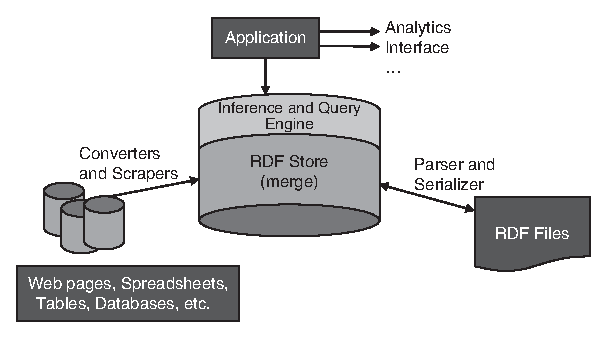
\includegraphics[width=5in]{media/ch7/f07-01.eps}
\caption{Semantic Web architecture with inferencing.}
\label{fig:ch7.1}
\end{figure}

The novelty of this architecture is an inferencing capability that
stands with the query component between the application and the RDF data
store. The power of a query engine with inferencing capability is
determined by the set of inferences that it supports. An RDFS inference
query engine supports a small set of inferences defined in the RDFS
standard; an OWL inference query engine supports the larger set of OWL
inferences. (Note that there are alternative formulations where the data
are pre-processed by an inferencing engine and then queried directly. We
discuss this later in this chapter.)

\begin{example}{Simple RDFS Query}
\label{ex:7.1}

Suppose we have an inference engine that includes support for the type
propagation rule working over an RDF
store that contains only these two triples:

\begin{lstlisting}
shop:Henleys rdfs:subClassOf shop:Shirts. 
shop:ChamoisHenley rdf:type shop:Henleys.
\end{lstlisting}

Suppose we have a SPARQL triple pattern that we use to examine these
triples, thus:

\textbf{Ask:}

\begin{lstlisting}
SELECT ?item
WHERE {?item rdf:type shop:Shirts . }
\end{lstlisting}

In a plain RDF query situation, this pattern will match no triples
because there is no triple with predicate rdf:type and object
shop:Shirts. However, since the RDFS inference standard includes the
type propagation rule just listed, with an RDFS inferencing query
engine, the following single result will be returned:

\textbf{Answer:}

\begin{tabular}{|l|}
\hline
?item\\
\hline
Shop:ChamoisHenley\\
\hline
\end{tabular}

\subsection{Asserted triples versus inferred triples}

It is often convenient to think about inferencing and queries as
separate processes, in which an inference engine produces all the
possible inferred triples, based on a particular set of inference rules.
Then, in a separate pass, an ordinary SPARQL query engine runs over the
resulting augmented triple store. It then becomes meaningful to speak of
\emph{asserted triples} versus \emph{inferred triples}.

Asserted triples, as the name suggests, are the triples that were
asserted in the original RDF store. In the case where the store was
populated by merging triples from many sources, all the triples are
asserted. Inferred triples are the additional triples that are inferred
by one of the inference rules that govern a particular inference engine.
It is, of course, possible for the inference engine to infer a triple
that has already been asserted. In this case, we still consider the
triple to have been asserted. It is important to note that there is no
logical distinction between inferred and asserted triples, the inference
engine will draw exactly the same conclusions from an inferred triple as
it would have done, had that same triple been asserted.
\end{example}

\begin{example}{Asserted versus Inferred Triples}

Even with a single inference rule like the type propagation rule, we can
show the distinction of asserted vs. inferred triples. Suppose we have
the following triples in a triple store:

\begin{lstlisting}
shop:Henleys rdfs:subClassOf shop:Shirts. 
shop:Shirts rdfs:subClassOf shop:MensWear. 
shop:Blouses rdfs:subClassOf shop:WomensWear.
shop:Oxfords rdfs:subClassOf shop:Shirts. 
shop:Tshirts rdfs:subClassOf shop:Shirts. 
shop:ChamoisHenley rdf:type shop:Henleys.
shop:ClassicOxford rdf:type shop:Oxfords. 
shop:BikerT rdf:type shop:Tshirts.
\end{lstlisting}

These triples are shown graphically in Figure~\ref{fig:ch7.2}.

\begin{figure}
\centering
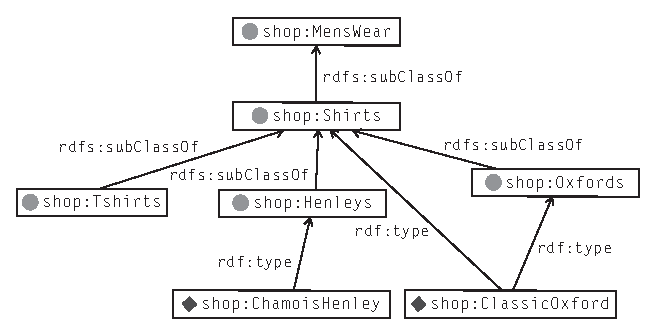
\includegraphics[width=5in]{media/ch7/f07-02.eps}
\caption{Asserted triples in the catalog model.}
\label{fig:ch7.2}
\end{figure}

An inferencing query engine that enforces just the type propagation rule
will draw the following inferences (for the purpose of these examples, an asterisk denotes an inferred triple):

\begin{lstlisting}
*shop:ChamoisHenley rdf:type shop:Shirts .
*shop:ChamoisHenley rdf:type shop:MensWear .
*shop:ClassicOxford rdf:type shop:Shirts .
*shop:ClassicOxford rdf:type shop:MensWear .
*shop:BikerT rdf:type shop:Shirts .
*shop:BikerT rdf:type shop:MensWear .
\end{lstlisting}

\begin{figure}
\centering
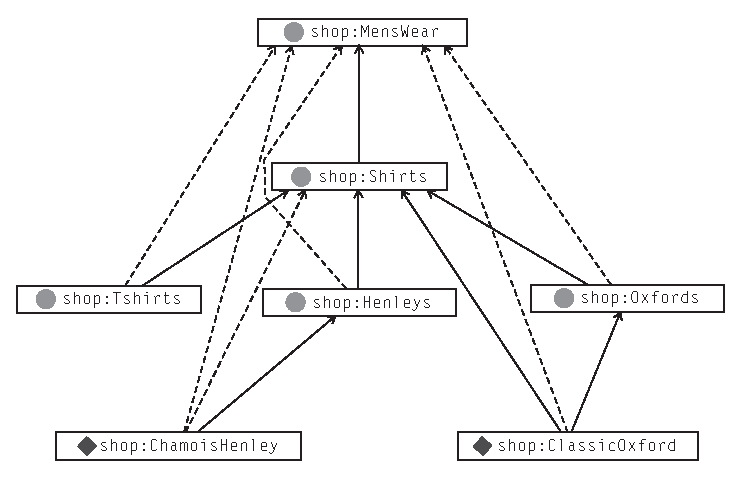
\includegraphics[width=5in]{media/ch7/f07-03.eps}
\caption{All triples in the catalog model. Inferred triples are shown as dashed
lines.}
\label{fig:ch7.3}
\end{figure}



Some of these triples were also asserted; the complete set of triples
over which queries will take place is as follows, with inferred triples
in italics:

\begin{lstlisting}
shop:Henleys rdfs:subClassOf shop:Shirts.
shop:Shirts rdfs:subClassOf shop:MensWear.
shop:Blouses rdfs:subClassOf shop:WomensWear.
shop:Oxfords rdfs:subClassOf shop:Shirts.
shop:TShirts rdfs:subClassOf shop:Shirts.
shop:ChamoisHenley rdf:type shop:Henleys.
*shop:ChamoisHenley rdf:type shop:Shirts.
*shop:ChamoisHenley rdf:type shop:MensWear.
shop:ClassicOxford rdf:type shop:Oxfords.
shop:ClassicOxford rdf:type shop:Shirts.
*shop:ClassicOxford rdf:type shop:MensWear.
shop:BikerT rdf:type shop:Tshirts.
*shop:BikerT rdf:type shop:Shirts.
shop:BikerT rdf:type shop:MensWear.
\end{lstlisting}

All triples in the model, both asserted and inferred, are shown in
Figure\ref{fig:ch7.3}. We use the convention that asserted triples are printed with
unbroken lines, and inferred triples are printed with dashed lines. This
convention is used throughout the book.
\end{example}

The situation can become a bit more subtle when we begin to merge
information from multiple sources in which each source itself is a
system that includes an inference engine. Most RDF implementations
provide a capability by which new triples can be asserted directly in
the triple store. This makes it quite straightforward for an application
to assert any or all inferred triples. If those triples are then
serialized (say, in RDF/XML) and shared on the Web, another application
could merge them with other sources and draw further inferences. In
complex situations like this, the simple distinction of asserted versus
inferred might be too coarse to be a useful description of what is
happening in the system.

\section{When Does Inferencing Happen?}

The RDFS and OWL standards define what inferences are valid, given
certain patterns of triples. But when does inferencing happen? Is
inferencing done at all? Where and how are inferred triples stored, if
at all? How many of them are there?

These questions are properly outside the range of the definitions of
RDFS and OWL, but they are clearly important for any implementation that
conforms to these standards. It should, therefore, come as no surprise
that the answers to these questions can differ from one implementation
to another. The simplest approach is to store all triples in a single
store, regardless of whether they are asserted or inferred. As soon as a
pattern is identified, any inferred triples are inserted into the store.
We will call this \emph{cached inferencing}, since all inferences are
stored (``cached'') with the data. This approach is quite simple to
describe and implement but risks an explosion of triples in the triple
store. At the other extreme, an implementation could instead never
actually store any inferred triples in any persistent store at all.
Inferencing is done in response to queries only. We will call this
\emph{just in time inferencing}, since the inferences are computed at
the latest possible moment. The query responses are produced in such a
way as to respect all the appropriate inferences, but no inferred triple
is retained. This method risks duplicating inference work, but it is
parsimonious in terms of persistent storage. These different approaches
have an important impact in terms of change management. What happens if
a data source changes---that is, a new triple is added to some data
store or a triple is removed? A strategy that persistently saves
inferences will have to decide which inferred triples must also be
removed. This presents a difficult problem, since it is possible that
there could be many ways for a triple to be inferred. Just because one
inference has been undermined by the removal of a triple, does that mean
that it is appropriate to remove that triple? An approach that
recomputes all inferences whenever a query is made need not face this
issue.

An important variant of just in time inferencing is where no explicit
inferencing is done at all. We already saw, in our example about
subclasses of Shirts, how a query could explicitly express what data it
wanted, without relying on the inference semantics of the model at all.
As we see in the next section, even in this case, where there is no
explicit inferencing, the inference interpretation of a model is still
important in organizing and understanding a semantic application.

\subsection{Inferencing as specification}

At the beginning of this chapter, we looked at a query to find all the
Shirts in a catalog, explicitly tracing down the all \texttt{rdfs:subClassOf}
links:

\begin{lstlisting}
SELECT ?item
WHERE {?class rdfs:subClassOf* :Shirts .
?item a ?class . }
\end{lstlisting}

This selection was done to support a search operation---``find me all
the Shirts.'' This query operates without any explicit reference to
inference at all; it returns its answers without reference to inferred
triples vs. asserted triples; it just processes the asserted data. But
how do we know that the items returned by this query are Shirts?

This same question could be asked of a program in Java or C++ or even
SQL---if we write a program to collect up the members of all the
subclasses of Shirts (and their subclasses, and so on), do we know that
all the things we have collected are Shirts? If we return one of these
things as the result of a user search, can we be justified in thinking
that it is itself a shirt? This suggests a role that a semantic model
can play in the interpretation of data---it can tell us whether the
queries we have written are correct. In this example, our model tells us
that every Henley is a shirt, because the class Henleys is a subclass of
the class Shirts. The same goes for Oxfords, and for any subclasses of
Oxfords. The model, along with its formal semantics, guarantees that all
the results of this query will indeed be shirts.

In this sense, the model is a specification. Any discussion about the
appropriateness of a particular query can appeal to the model for
arbitration---is this query consistent with the model? In this example,
the model tells us that any result from this query will be a Shirt, so
it is appropriate to treat them as such. When the model is written in a
language for which there is a capability to do automated inferences
(like RDFS, RDFS-Plus, or OWL), it becomes particularly useful---the
specification is said to be executable. This means that we can run a
program that will tell us exactly what the model means. In the example
above where we showed asserted and inferred triples, we showed the
results of just such a capability, resulting in a list of all the Shirts
(of any type).

When building an application, we might decide to use a general-purpose
inference capability, or we might decide to use an extended query (like
the one shown here), or we might write a program in some other language.
A specification (even an executable one) tells us what our program or
query ought to do; it doesn't tell us how we should do it. Regardless of
this implementation choice, the model plays a central role of justifying
the query or program. If many people develop different systems (even
using different technological approaches), the results they provide will
be consistent, if they justify them all against the same model.


\section{Expectation in RDF}


In Chapter~\ref{ch1}, we examined some of the assumptions around managing information on the web, 
whether it is to be consumed directly by humans or first by machines.  One of the basic assumptions is
that we cannot know, in advance, what we will find on the web, therefore, we must proceed with the \emph{Open World} assumption (Section~\ref{openworld}).  We only draw conclusions from data that will not be undermined or countermanded by the discovery of new data.  This assumption makes sense when we are interpreting data we find in the wild.

But there are some situations in which we are not interpreting data, we instead are acting on some expectations about the
data in the wild.  Our expectations about data might come from regulatory control (an application for a loan must
include certain information about the borrower), or our own business policies (we require certain information about a
prospective borrower before we will consider a loan), or just plain common sense (a borrow's date of birth cannot be in
the future).

Expectations in the Semantic Web can take three broad forms:

\begin{itemize}
    \item \emph{Data Validation} \label{datav} Data found in the wild purports to describe a particular kind of thing, and we have
    expectations about that type.  We want to validate that the data matches our expectations.

  \item \emph{Soliciting user input} \label{form}
      We might not find our data published on the web as a linked data resource, but
      rather, we want to request input from a user.  In this case, we want to be able to communicate to that user what
      our expectations are for the data they will provide.  This is typically done with a form or a wizard that a user
      fills out with the data they are providing.

    \item \emph{Validating user input} \label{userv} Even when we have communicated our expectations to a user,
      they might not provide 
      data in the form we expect.  In this case, just as in the first case, we will want to validate our data against our
      expectations.
\end{itemize}

We can think of our expectations for a data description as a specification of the \emph{shape} that the data should take.  This metaphor is quite literal in case \ref{form} above, where the expected shape of the data is presented in a form that a user will fill out.  

Beyond the shape of a data description, our expectations can also place constraints on values.  The age of an adult must be greater than 18 (or 21, depending on the intent of the data shape in question);  a social security number must be of the form XXX-XX-XXXX.

These intuitions are the motivation behing the name of the expectation modeling language of the Semantic Web, \emph{SHACL}, Shapes Constraint Language.  SHACL provides a mechanism for specifying the expected shape of a data description and constraints on its validity.

We'll illustrate all three uses of SHACL with a single example, shown in Figure~\ref{fig:ch7.account}.

\begin{figure}
  \begin{lstlisting}
 1. @prefix sh: <http://www.w3.org/ns/shacl#> .
 2. account:Account
 3.   rdf:type sh:NodeShape ;
 4.   rdfs:label "Account" ;
 5.   sh:property [
 6.       rdf:type sh:PropertyShape ;
 7.       sh:path account:lastName ;
 8.       sh:datatype xsd:string ;
 9.       sh:name "family name" ;
10.       sh:description "the name shared by all members of a family" ;
11.       sh:maxCount 1 ] ;
12.   sh:property [
13.       rdf:type sh:PropertyShape ;
14.       sh:path account:ssn ;
15.       sh:datatype xsd:string ;
16.       sh:description
17.            "US Social Security Number - format XXX-XX-XXXX" ;
18.       sh:maxCount 1 ;
19.       sh:minCount 1 ;
20.       sh:name "SSN" ;
21.       sh:pattern
22.          "[0-9][0-9][0-9]-[0-9][0-9]-[0-9][0-9][0-9][0-9]" ] ;
23.   sh:property [
24.       sh:path account:gender ;
25.       sh:datatype xsd:string ;
26.       sh:in (
27.           "female"
28.           "male"
29.         ) ;
30.       sh:maxCount 1 ;
31.       sh:name "gender" ] .
  \end{lstlisting}
  \caption{Listing of a SHACL model for an Account}
  \label{fig:ch7.account}
\end{figure}

The first thing to notice about Figure~\ref{fig:ch7.account} is that it is expressed in RDF.  This is typical of the langauges of the Semantic Web; every language is expressed in RDF, so that the models in that language can be distirbuted across the web as linked data sets in their own right (see Chapter~\ref{ch5}. 

The second thing to notice is the large number of resources whose names
begin with \texttt{sh:}.  As we see in line 1, this is a prefix abbreviation for
\texttt{http://www.w3.org/ns/shacl\#}, which is a domain prefix controlled by the
W3C (as we saw in Section~\ref{minting-http-uris}).  This is also typical of how a
new language is built on top of RDF; the language publisher (in this case, the W3C)
defines a number of resources in a single domain that they control.  If you dereference
one of these HTTP URIs, the result (which is maintained by the same publisher, the W3C) is a 
description of that resource.  If you paste the HTTP URI 
\texttt{http://www.w3.org/ns/shacl\#} into a web browser, you will see the W3C 
Recommendation document that describes SHACL.


Now let's dive into the details of the shapes.  
In the data, we have three entities that claim to be \texttt{Accounts}.  For
each of them, certain data is provided; first names, last names, SSN, gender.
The shapes in Figure~\ref{fig:ch7.account} specifies our expectations about these
things.

There are three constraints on properties defined in Figure~\ref{fig:ch7.account}, beginning on lines 5, 12 and 23.  The property that they place a constraint on is given by \texttt{sh:path}, so they constrain \texttt{account:lastName} (line 7), \texttt{account:ssn} (ine 14)  and \texttt{account:gender} (line 24) respectively.

Each of these constraints say something different about the property.  
In the case of \texttt{account:lastName} (lines 5-11), the constraint says 
that the value must be a string,  and that there can be at most one value.

In the case of \texttt{account:ssn} (lines 12-22), there must be exactly one value 
(both min and max of 1 are specified), it must be a string, but it also must match
a pattern given by a regular expression.  Regular expressions are beyond the scope
of this book, but this one says that the string must have the form ``XXX-XX-XXXX''
where each X is a digit from 0 to 9.

Finally, the third contraint, on \texttt{account:gender} (lines 23-31) specifies that
there can be at most one value, and that value must be in the list given, that is, one
of ``male'' or ``female''.

\hypertarget{validating-data}{%
\subsection{Validating data}\label{validating-data}}


Let's see how this works, first in the context
of data validation.  Suppose we have data about the active accounts as shown in
Figure~\ref{fig:ch7.data}.


\begin{figure}
  \begin{lstlisting}
active:Account_1
  rdf:type account:Account ;
  rdfs:label "Account 1" ;
  account:firstName "Aaron" ;
  account:gender "male" ;
  account:lastName "Beatte" ;
  account:ssn "123-45-6789" .

active:Account_2
  rdf:type account:Account ;
  rdfs:label "Account 2" ;
  account:firstName "George" ;
  account:gender "unknown" ;
  account:lastName "Deller" ;
  account:ssn "12-345678" .

active:Account_3
  rdf:type account:Account ;
  rdfs:label "Account 3" ;
  account:firstName "Edelyn" ;
  account:lastName "Zetta" .
  \end{lstlisting}
\label{fig:ch7.data}
\caption{Data to be vaidated by Figure~\protect\ref{fig:ch7.account}.}
\end{figure}

First off, each descriptions in Figure~\ref{fig:ch7.data} has a single string value for
\texttt{account:lastName}, as expected.  So there is no violation in this data set for \texttt{lastName}.

Now let's look at \texttt{account:gender}.  \texttt{Account\_1} has the
value ``male'', which is one of the expected values, so there is no
violation.  \texttt{Account\_2} has the value ``unknown'' for \texttt{account:gender}.  This is not one 
of the expected values, so this is a violation.  SHACL can be quite specific about
the violation - the given value, ``unknown'', is not in the list of allowed
values (``female'', ``male'').  \texttt{Account\_3}, on the other hand, has 
no value at all for \texttt{account:gender}.  The constraint says that the
maximum number of values we can have for this property is 1, but says nothing about the
minimum number of values.  So, according to this shape, the correct way to specify
an unknown gender (or an unwillingness to provide one from the list ``male''
and ``female'') is to leave it out. 

The constraint on \texttt{account:ssn} specifies a pattern that a SSN should take.
In our data, \texttt{active:Account\_1} specifies a SSN of the appropriate format.
\texttt{active:Account\_2} specifies an SSN, but the format does not match.  SHACL can
be very specific about the violation, that the value for \texttt{account:ssn}
does not match the pattern given in the shape.  Finally, \texttt{active:Account\_3}  provides no value for SSN at all.  In this case, the shape specifies (line 18, Figure~\ref{fig:ch7.account}) \texttt{sh:minCount 1}, so, unlike the case of the missing
gender, this is a violation, namely, property needs at least 1 value, found 0.

The process we just outlined is called \emph{SHACL validation}; given a set of
shape defintions in SHACL, and data that purports to conform to those shapes,
we can automatically determine whether and how the data violates the constraints
given in the shape.

Validation is important in the web of data, since the applications
that publish and consume data from the Web of data are  written and
hosted by different organizations.  if we want to ensure
interoperability between open and heterogeneous systems, we need a way
to specify our expectations about the data they will provide and
consume.  SHACL provides a way to specify those expectations, and
SHACL validation provides a way to enforce them.



\subsection{Soliciting User Input}\label{soliciting}

The same constraints that allow us to validate data can be used to
control the solicitation of data from a user.  Take the shape given in
Figure~\ref{fig:ch7.account}.  Just intuitively, if we wanted to make
a form for a user to fill out, we would expect the form to have three
fields, one each for \texttt{account:lastName}, \texttt{account:ssn}
and \texttt{account:gender}.  But we of course don't expect a form to
use the QName of a property to elicit input.  Fortunatlely,
Figure~\ref{fig:ch7.account} also provides names for each of the
constraints, and these names are more suitable for human consumption;
``family name'', ``SSN'' and ``gender''.  If further information is
needed about any of these things (e.g., what does SSN stand for?),
there is the \texttt{sh:description}, which describes it in more
detail.  In the case of \texttt{account:gender}, the constraint even
provides a suggestion for how the form should operate; it should only
provide two options for the answer, corresponding to the two
accpetable answers, ``male'' and ``female''.

There are any number of technologies avaiable for producing forms for
people to fill in; SHACL simply provides the content, in terms of
field names, types, and allowable values that the forms should have.
Figure~\ref{fig.ch7.form} shows an example form created from the shape
in Figure~\ref{fig.ch7.account}, using basic HTML.



\subsection{Validating User Input}\label{vuser}

One of the advantages of using a machine-readable shapes language like
SHACL (remember, SHACL is in RDF, so we can query over it using
SPARQL, as we saw in Chapter~\ref{ch6}) is that we can use the same
model (Figure~\ref{fig.ch7.account}) to drive data validation
(Section~\ref{validating-data}) as we use to solicit data from human
users (Section~\ref{soliciting}).  We can combine these processes, and
use the same model to validate user input.

We've already seen that the model can be used to prevent certain data
errors by users.  By buiding a form that only accepts values ``male''
and ``female'', we prevent a user from submitting a form with a value
like ``unknown''.  But, depending on the technology we are using for
the forms, we might not be able to enforce all of the constraints
expressed in a shape with a form.

For example, the constraint on SSN is somewhat elaborate; it requires
something that can check a regular expression against the human
input.  Simple HTML forms don't have a facility for regular
expressions, so we just have to leave it to the human to fill in the
form, and hope that they follow the format suggestion given in the
\texttt{sh:description} field of the shape.

Once we have the results from the form, we can process it using the
same tool that we used for data on the web, namely, a SHACL
validator. This allows us to make sure that the data entered by a
human user will conform to the same high standard as data we find on
the web.

In this way, SHACL helps us to retain the value of the data wilderness
while, to some extent, taming its wild nature.  We still accept data
from across the web, we still allow anyone to say anything about any
topic, but we protect our data applications from runaway behavior by
enforcing shapes and constraints on the data.


\section{SUMMARY}

RDF provides a way to represent data so that information from multiple
sources can be brought together and treated as if they came from a
single source. But when we want to use that data, the differences in
those sources comes out. For instance, we'd like to be able to write a
single query that can fetch related data from all the integrated data
sources.

The Semantic Web provides an approach to this problem in the form of
modeling languages in which the relationship between data sources can be
described. A modeling construct's meaning is given by the pattern of
inferences that can be drawn from it. Information integration can be
achieved by invoking inferencing before or during the query process; a
query returns not only the asserted data but also inferred information.
This inferred information can draw on more than one data source.

We have seen how even very simple inferencing can provide value for data
integration. But just exactly what kind of inferencing is needed? There
isn't a single universal answer to this question. The

Semantic Web standards identify a number of different levels of
expressivity, each supporting different inferences, and intended for
different levels of sophistication of data integration over the Semantic
Web.

In the following chapters, we will explore three particular inferencing
levels. They differ only in terms of the inferences that each of the
languages allow. RDFS (Chapter 6) is a recommendation defined and
maintained by the W3C. It operates on a small number of inference rules
that deal mostly with relating classes to subclasses and properties to
classes. RDFS-PLUS (Chapter 7) is a mode that we have defined for this
book. We have found a particular set of inference patterns to be helpful
both pedagogically (as a gentle introduction to the more complex
inference patterns of OWL) and practically (as a useful integration tool
in its own right). RDFS-PLUS builds on top of RDFS to include
constraints on properties and notions of equality. OWL (Chapters 9 and
10) is a recommendation defined and maintained by the W3C, which builds
further to include rules for describing classes based on allowed values
for properties. All of these standards use the notion of inferencing to
describe the meaning of a model; they differ in the inferencing that
they support.

\subsection{Fundamental concepts}

The following fundamental concepts were introduced in this chapter.

\begin{itemize}
\item Inferencing---The process by which new triples are systematically added
to a graph based on patterns in existing triples.

\item Asserted triples---The triples in a graph that were provided by some
data source.

\item Inferred triples---Triples that were added to a model based on
systematic inference patterns.

\item Inference rules---Systematic patterns defining which of the triples
should be inferred.

\item Inference engine---A program that performs inferences according to some
inference rules. It is often integrated with a query engine.

\item
  SHACL shapes to validate RDF data at the structural level by providing
  the constraint you expect them to meet.
  \end{itemize}
  

\chapter{RDF Schema}
\label{ch8}

Just as Semantic Web modeling in RDF is about graphs, Semantic Web
modeling in the RDF Schema Language (RDFS) is about sets. Some aspects
of set membership can be modeled in RDF alone, as we have seen with the
\texttt{rdf:type} built-in property. But RDF itself simply creates a graph
structure to represent data. RDFS provides some guidelines about how to
use this graph structure in a disciplined and standardized way. It
provides a way to talk about the vocabulary that will be used in an RDF
graph. Which individuals are related to one another, and how? How are
the properties we use to define our individuals related to other sets of
individuals and, indeed, to one another? RDFS provides a way for an
information modeler to express the answers to these sorts of questions
as they pertain to particular data modeling and integration needs.

As such, RDFS is like other schema languages: It provides information
about the ways in which we describe our data. But RDFS differs from
other schema languages in important ways.

\section{Schema Languages and their Functions}

RDFS is the schema language for RDF. But what is a schema language in
the first place? There are a number of successful schema languages for
familiar technologies, but the role that each of these languages play in
the management of information is closely tied to the particular language
or system.

Let's consider document modeling systems as an example. For such a
system, a schema language allows one to express the set of allowed
formats for a document. For a given schema, it is possible to determine
(often automatically) whether a particular document conforms to that
schema. This is the major capability provided by XML Schema definitions.
XML parsers can automatically determine whether a particular XML
document conforms to a given schema.

Other schema languages help us to interpret particular data. For
example, a database schema
provides header and key information for tables in a relational database.
There is neither anything in the table itself to indicate the meaning of
the information in a particular column nor anything to indicate which
column is to be used as an index for the table. This information is
appropriately included in the database schema, since it does not change
from one data record to the next.

For Object-Oriented Programming systems, the class structure plays an
organizing role for information as well. But in object-oriented
programming, the class diagram does more than describe data. It
determines, according to the inheritance policy of the particular
language, what methods are available for a particular instance and how
they are implemented. This stands in stark contrast to relational
databases and XML, in that it does not interpret information but instead
provides a systematic way for someone to describe information and
available transformations for that information.

Given this variety of understandings of how schema information can be
used in different modeling paradigms, one might wonder whether calling
something a schema language actually tells us anything at all! But there
is something in common among all these notions of a schema. In all
cases, the schema tells us something about the information that is
expressed in the system. The schema is information about the data.

How then can we understand the notion of schema in RDF? What might we
want to say about RDF data? And how might we want to say it? The key
idea of the schema in RDF is that it should help provide some sense of
meaning to the data. It accomplishes this by specifying semantics using
inference patterns.

\subsection{Relationship between schema and data}

In most modeling systems, there is a clear division between the data and
its schema. The schema for a relational database is not typically
expressed in a table in the database; the object model of an
object-oriented system is not expressed as objects, and an XML DTD \footnote{DTD was the original 
document type definition format for XML} is
not a valid XML document.

But in many cases, modern versions of such systems do model the schema
in the same form as the data; the meta-object protocol of Common Lisp
and the introspection API of Java represent the object models as objects
themselves. The XML Stylesheet Definition (XSD) \footnote {XSD is the modern way to define XML schemas} 
defines XML Styles in an XML
language.

In the case of RDF, the schema language was defined in RDF from the very
beginning. That is, all schema information in RDFS is defined with RDF
triples. The relationship between ``plain'' resources in RDF and schema
resources is made with triples, just like relationships between any
other resources. This elegance of design makes it particularly easy to
provide a formal description of the semantics of RDFS, simply by
providing inference rules that work over patterns of triples. While this
is good engineering practice (in some sense, the RDF standards committee
learned a lesson from the issues that the XML standards had with DTDs),
its significance goes well beyond its value as good engineering. In RDF,
everything is expressed as triples. The meaning of asserted triples is
expressed in new (inferred) triples. The structures that drive these
inferences, that describe the meaning of our data, are also in triples.
This means that this process can continue as far as it needs to; the
schema information that provides context for information on the Semantic
Web can itself be distributed on the Semantic Web. This also means that
every tool and technique available for RDF data is available for RDFS
schemas: you can query a schema in SPARQL, validate it in SHACL, edit
it in an RDF editor, publish it with Linked Data practices and tools,
visualize it with an RDF visualizer, etc.

We can see this in action by showing how a set is defined in RDFS. The
basic construct for specifying a set in RDFS is called an \texttt{rdfs:Class}.
Since RDFS is expressed in RDF, the way we express that something is a
class is with a triple---in particular, a triple in which the predicate
is \texttt{rdf:type}, and the object is \texttt{rdfs:Class}. Here are some examples that
we will use in the following discussion:

\begin{lstlisting}
:AllStarPlayer rdf:type rdfs:Class .
:MajorLeaguePlayer rdf:type rdfs:Class .
:Surgeon rdf:type rdfs:Class .
:Staff rdf:type rdfs:Class .
:Physician rdf:type rdfs:Class .
\end{lstlisting}

These are triples in RDF just like any other; the only way we know that
they refer to the schema rather than the data is because of the use of
the term in the \texttt{rdfs:} namespace, \texttt{rdfs:Class}. But what is new here? In
Chapter~\ref{ch3}, we already discussed the notion of \texttt{rdf:type}, which we used to
specify that something was a member of a set. What do we gain by
specifying explicitly that something is a set? We gain a description of
the meaning of membership in a set. In RDF, the only ``meaning'' we had
for set membership was given by the results of some query; \texttt{rdf:type}
actually didn't behave any differently from any other (even
user-defined) property. How can we specify what we mean by set
membership? In RDFS, we express meaning through the mechanism of
inference.

\section{The RDF Schema Language}

RDFS ``extends'' RDF by introducing a set of distinguished resources
into the language. This is similar to the way in which a traditional
programming language can be extended by defining new language- defined
keywords. But there is an important difference: In RDF, we already had
the capability to use
any resource in any triple (Anyone can say Anything about Any topic). So
by identifying certain specific resources as ``new keywords,'' we
haven't actually extended the language at all! We have simply identified
certain triples as having a special meaning, as defined by a standard.

How can we define the ``meaning'' of a distinguished resource? As we saw
in Chapter~\ref{ch7}, in RDFS, meaning is expressed by specifying inferences
that can be drawn when the resource is used in a certain way. Throughout
the rest of this section, whenever we introduce a new RDFS resource, we
will answer the question ``What does it mean?'' with an answer of the
form ``In these circumstances (defined by some pattern of triples), you
can add (infer) the following new triples.'' We already saw how to do
this with the type propagation rule for \texttt{rdfs:subClassOf}; now we will
demonstrate this principle using another of the most fundamental terms
in RDFS: \texttt{rdfs:subPropertyOf}.

\subsection{Relationship propagation through rdfs:subPropertyOf}

The basic intuition behind the use of \texttt{rdfs:subPropertyOf} is that
terminology includes verbs as well as nouns, and many of the same
requirements for mapping nouns from one source to another will apply to
relationships. Simple examples abound in ordinary parlance. The
relationship brother is more specific than the relationship sibling; if
someone is my brother, then he is also my sibling. This is formalized in
RDFS for \texttt{rdfs:subPropertyOf} using an inference rule that is almost as
simple as the one for \texttt{rdfs:subClassOf}.

\begin{lstlisting}
CONSTRUCT {?x ?r ?y .}
WHERE {?x ?q ?y .
       ?q rdfs:subPropertyOf ?r }
\end{lstlisting}

That is, in any triple, we can replace the predicate with any property
it is a \texttt{subPropertyOf}.

\begin{example}{Employment}

A large firm engages a number of people in various capacities and has a
variety of ways to administer these relationships. Some people are
directly employed by the firm, whereas others are contractors. Among
these contractors, some of them are directly contracted to the company
on a freelance basis, others on a long-term retainer, and still others
contract through an intermediate firm. All of these people could be said
to work for the firm.

How can we model this situation in RDFS? First, we need to consider the
inferences we wish to be able to
draw and under what circumstances. There are a number of relationships
that can hold between a person and the firm; we can call them
\texttt{contractsTo}, \texttt{freeLancesTo}, \texttt{indirectlyContractsTo}, \texttt{isEmployedBy}, and
\texttt{worksFor}.

If we assert any of these statements about some person, then we would
like to infer that that person
\texttt{worksFor} the firm. Furthermore, there are intermediate conclusions we
can draw---for instance, both a freelancer and an indirect contractor
contract to the firm and indeed work for the firm.

All these relationships can be expressed in RDFS using the
\texttt{rdfs:subPropertyOf} relation:

\begin{lstlisting}
:freeLancesTo rdfs:subPropertyOf contractsTo .
:indirectlyContractsTo rdfs:subPropertyOf contractsTo .
:isEmployedBy rdfs:subPropertyOf worksFor .
:contractsTo rdfs:subPropertyOf worksFor .
\end{lstlisting}

\begin{figure}
\centering
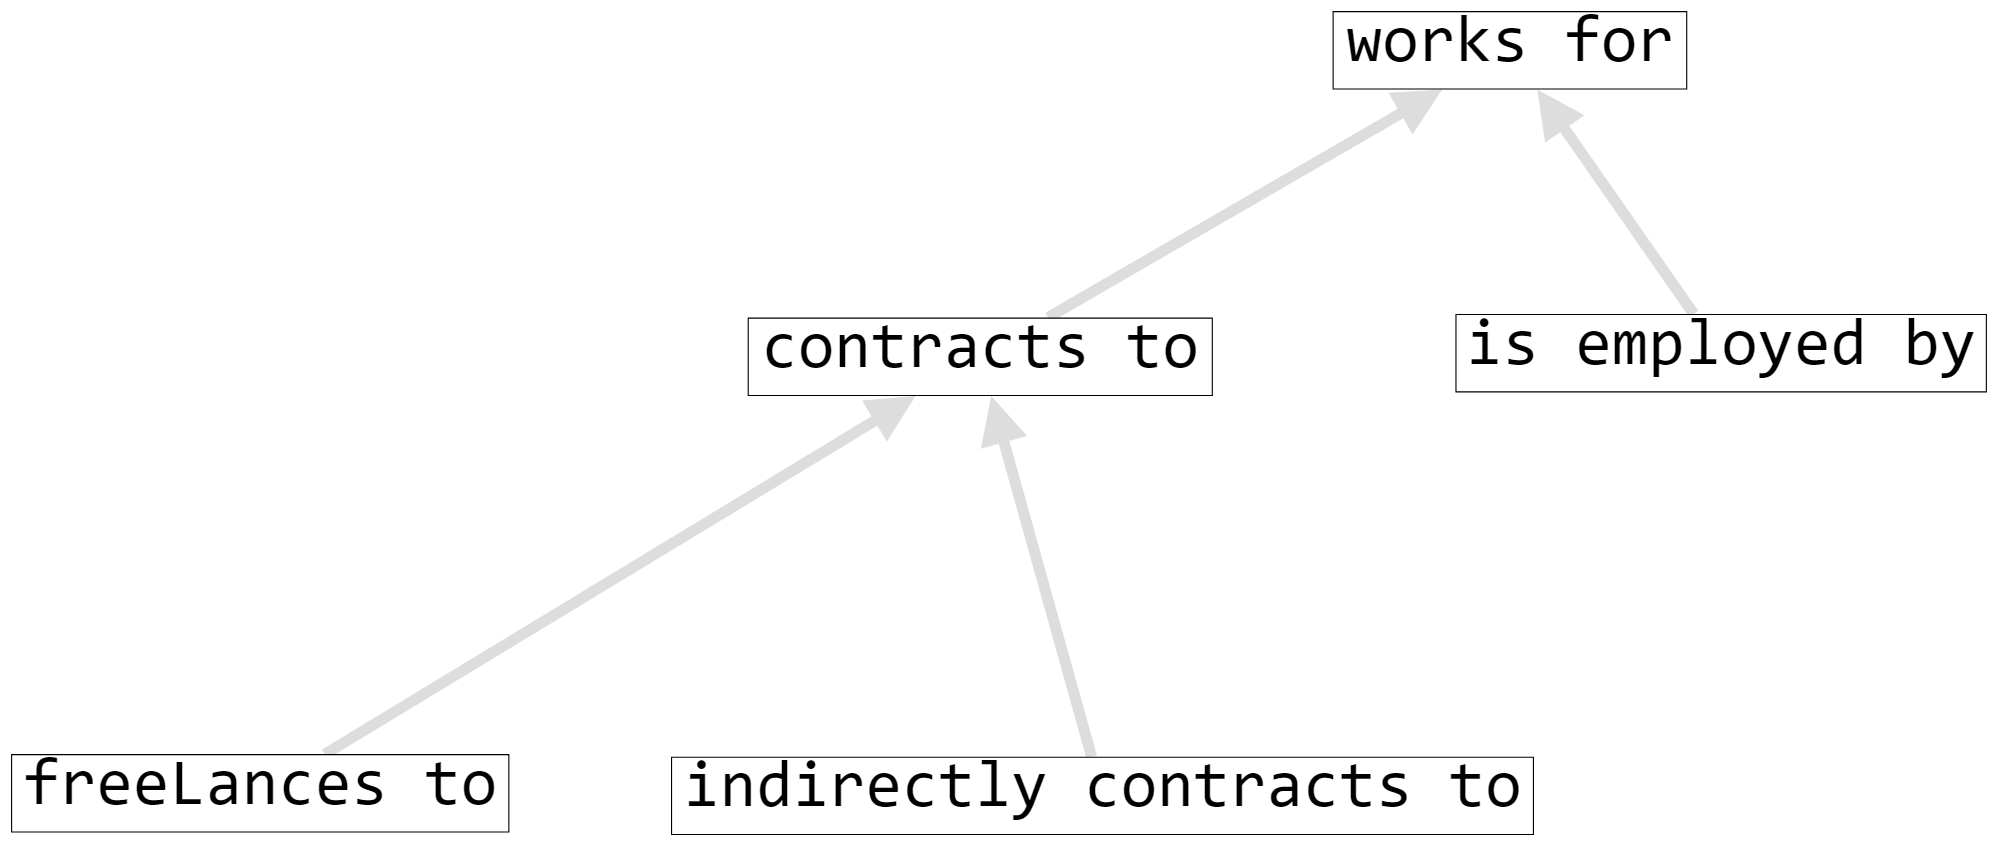
\includegraphics[width=5in]{SWWOv3/media/ch8/figure8-1.png}
\caption{rdfs:subPropertyOf relations for workers in the firm.}
\label{fig:ch8.1}
\end{figure}


The discussion will be easier to follow if we represent this as a
diagram, where the arrows denote
\texttt{rdfs:subPropertyOf} (see Figure~\ref{fig:ch8.1}).

To see what inferences can be drawn, we will need some instance data:

\begin{lstlisting}
:Goldman :isEmployedBy :TheFirm .
:Spence :freeLancesTo :TheFirm .
:Long :indirectlyContractsTo :TheFirm .
\end{lstlisting}

The rule that defines the meaning of \texttt{rdfs:subPropertyOf} implies a new
triple, replacing any sub- property with its superproperty. So, since

\begin{lstlisting}
:isEmployedBy :rdfs:subPropertyOf :worksFor.
\end{lstlisting}

we can infer that

\begin{lstlisting}
* :Goldman :worksFor :TheFirm.
\end{lstlisting}

And because of the assertions about freelancing and indirect contracts,
we can infer that

\begin{lstlisting}
* :Spence :contractsTo :TheFirm .
* :Long contractsTo :TheFirm .
\end{lstlisting}

And finally, since, like asserted triples, inferred triples can be used
to make further inferences, we can further infer that

\begin{lstlisting}
* :Spence :worksFor :TheFirm .
* :Long :worksFor :TheFirm .
\end{lstlisting}

In general, \texttt{rdfs:subPropertyOf} allows a modeler to describe a hierarchy
of related properties. Just as in class hierarchies, specific properties
are at the bottom of the tree, and more general properties are higher up
in the tree. Whenever any property in the tree holds between two
entities, so does every property above it.
\end{example}

\begin{sidebar}{OO Comparison}
The construct \texttt{rdfs:subPropertyOf} has no direct analog in object-oriented
programming, where properties are not first-class entities (i.e., they
cannot be related to one another, independent of the class in which they
are defined). For this reason, unlike the case of \texttt{rdfs:subClassOf},
object-oriented programmers have no conflict with a similar known
concept. The only source of confusion is that subproperty diagrams like
the preceding one are sometimes mistaken for class diagrams.
\end{sidebar}

\subsection{Typing data by usage---rdfs:domain and rdfs:range}
\label{section:domainrange}

We have seen how inferences around \texttt{rdfs:subPropertyOf} can be used to
describe how two properties relate to each other. But when we describe
the usage of terms in our data, we would also like to represent how a
property is used relative to the defined classes. In particular, we
might want to say that when a property is used, the triple subject comes
from (i.e., has \texttt{rdf:type}) a certain class and that the object comes from
some other type. These two stipulations are expressed in RDFS with the
resources (keywords) \texttt{rdfs:domain} and \texttt{rdfs:range}, respectively.

In mathematics, the words \emph{domain} and \emph{range} (or \emph{co-domain}) are used to
refer to how a function (or more generally, a relation) can be used. The
domain of a function is the set of values for which it is defined, and
the range is the set of values it can take. In Real Analysis, for
instance, the relation \emph{squareroot} has the positive numbers as the domain
(since negative numbers don't have square roots in the reals), and all
reals as the range (since there are both positive and negative square
roots).

In RDFS, the properties \texttt{rdfs:domain} and \texttt{rdfs:range} have meanings
inspired by the mathematical uses of these words. A property p can have
an \texttt{rdfs:domain} and/or an \texttt{rdfs:range}. These are specified, as is
everything in RDF, via triples:

\begin{lstlisting}
:p rdfs:domain :D.
:p rdfs:range :R.
\end{lstlisting}

The informal interpretation of this is that the relation \texttt{p} relates
values from the class \texttt{D} to values from the class \texttt{R}. \texttt{D} and \texttt{R} need not be
disjoint, or even distinct.

The meaning of these terms is defined by the inferences that can be
drawn from them. RDFS
inferencing interprets domain with the inference rule:

\begin{lstlisting}
CONSTRUCT {?x rdf:type ?D .}
WHERE {?P rdfs:domain ?D .
       ?x ?P ?y .}
\end{lstlisting}

Similarly, range is defined with the rule

\begin{lstlisting}
CONSTRUCT {?y rdf:type ?D .}
WHERE {?P rdfs:range ?D .
       ?x ?P ?y .}
\end{lstlisting}

In RDFS, domain and range give some information about how the property P
is to be used; domain refers to the subject of any triple that uses P as
its predicate, and range refers to the object of any such triple. When
we assert that property P has domain D (respectively, range R), we are
saying that whenever we use the property P, we can infer that the
subject (respectively object) of that triple is
a member of the class D (respectively R). In short, domain and range
tell us how P is to be used. Rather than signaling an error if P is used
in a way that is apparently inconsistent with this declaration, RDFS
will infer the necessary type information to bring P into compliance
with its domain and range declarations.

In RDFS, there is no way to assert that a particular individual is not a
member of a particular class (contrast with OWL, Chapter~\ref{ch13}). In fact,
in RDFS, there is no notion of an incorrect or inconsistent inference.
This means that, unlike the case of XML Schema or SHACL shape, an RDF
Schema will never proclaim an input as invalid; it will simply infer
appropriate type information. In this way, RDFS behaves much more like a
database schema, which declares what joins are possible but makes no
statement about the validity of the joined data.

\subsection{Combination of domain and range with rdfs:subClassOf}

So far, we have seen inference patterns for some resources in the rdfs
namespace: \texttt{rdfs:domain}, \texttt{rdfs:range}, \texttt{rdfs:subPropertyOf}, and
\texttt{rdfs:subClassOf}. We have seen how the inference patterns work on sample
triples. But the inference patterns can also interact with one another
in interesting ways. We can already see this happening with the three
patterns we have seen so far. We will show the interaction between
\texttt{rdfs:subClassOf} and \texttt{rdfs:domain} by starting with an example.

Suppose we have a very simple class tree that includes just two classes,
\texttt{Woman} and \texttt{MarriedWoman}, in the usual subclass relation:

\begin{lstlisting}
:MarriedWoman rdfs:subClassOf :Woman.
\end{lstlisting}

Suppose we have a property called \texttt{hasMaidenName}, whose domain is
\texttt{MarriedWoman}:

\begin{lstlisting}
:hasMaidenName rdfs:domain :MarriedWoman.
\end{lstlisting}

Figure\ref{fig:ch8.2} shows how this looks in diagram form.

\begin{figure}
\centering
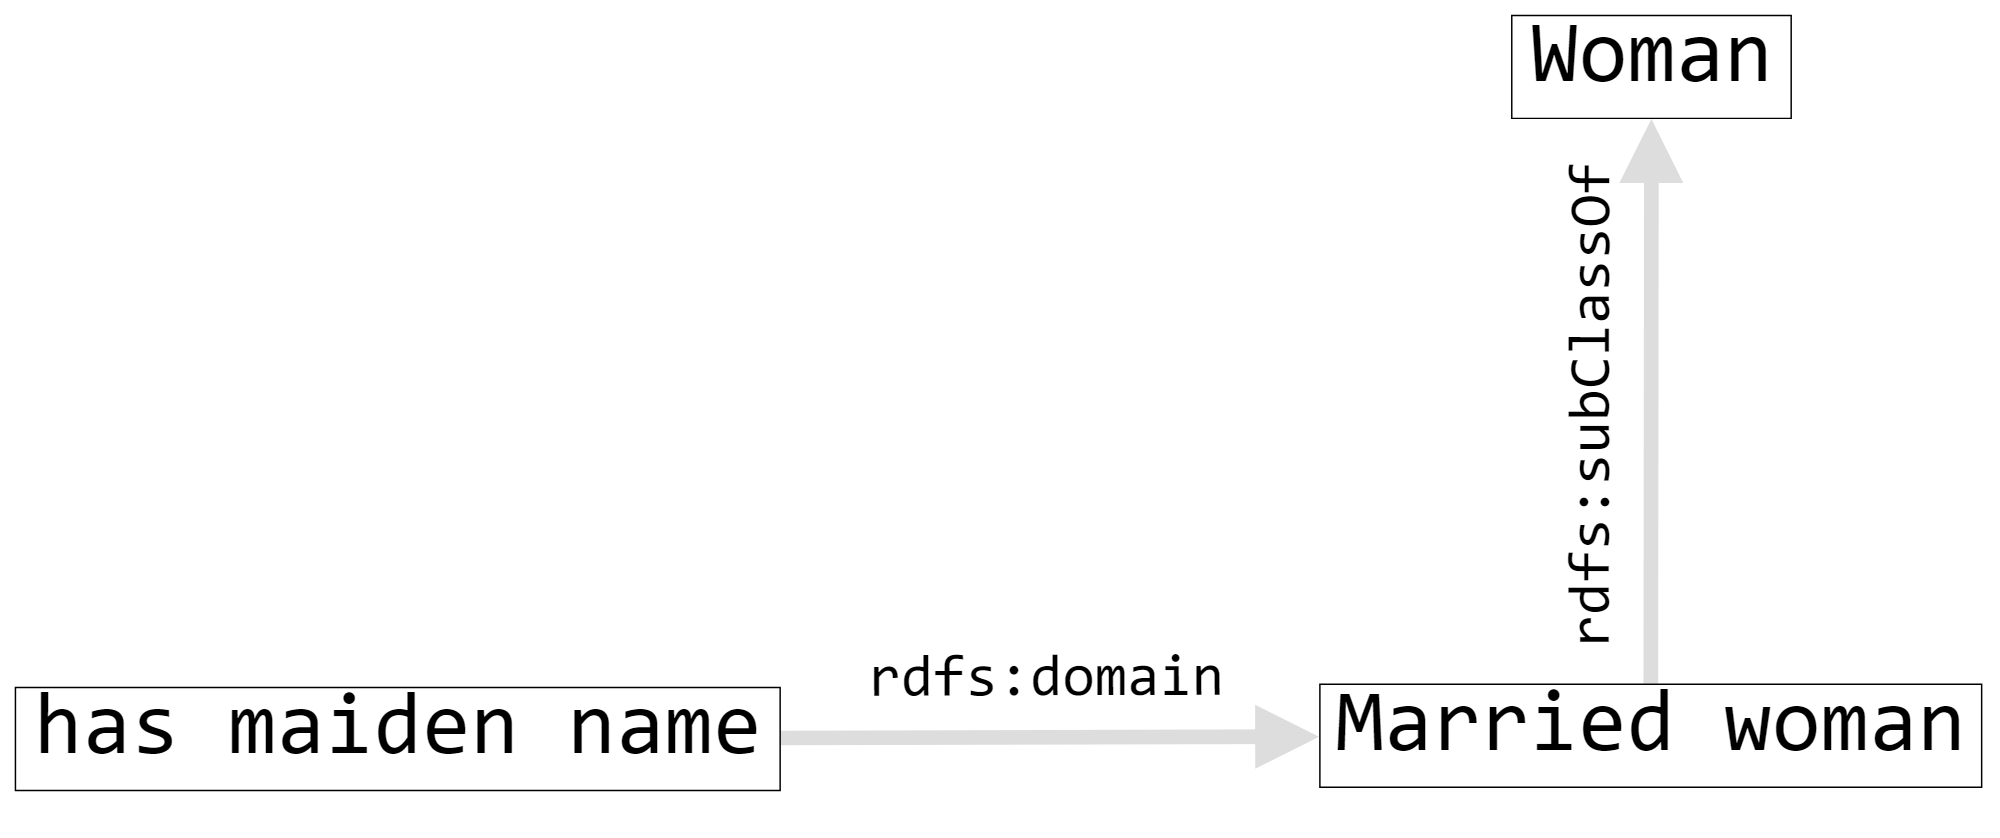
\includegraphics[width=5in]{SWWOv3/media/ch8/figure8-2.png}
\caption{Domain and subClassOf triples for hasMaidenName.}
\label{fig:ch8.2}
\end{figure}


This unsurprising model holds some subtlety; let's examine closely what
it says. If we assert the \texttt{hasMaidenName} of anything (even if we don't
know that it is a \texttt{Woman}!), the rule for \texttt{rdfs:domain} allows us to infer
that it is a \texttt{MarriedWoman}. So, for instance, if someone asserts

\begin{lstlisting}
:Karen :hasMaidenName "Smith" .
\end{lstlisting}

We can infer

\begin{lstlisting}
* :Karen rdf:type :MarriedWoman.
\end{lstlisting}

But we can make further inferences based on the \texttt{rdfs:subClassOf}
relationship between the classes---namely, that

\begin{lstlisting}
* :Karen rdf:type :Woman.
\end{lstlisting}

There was nothing in this example that was particular to Karen; in fact,
if we learn of any resource at all that it has a \texttt{hasMaidenName}, then we
will infer that it is a \texttt{Woman}. That is, we know that for any resource X,
if we have a triple of the form

\begin{lstlisting}
?X :hasMaidenName ?Y .
\end{lstlisting}

we can infer

\begin{lstlisting}
* ?X rdf:type :Woman.
\end{lstlisting}

But this is exactly the definition of \texttt{rdfs:domain}; that is, we have just
seen that

\begin{lstlisting}
:hasMaidenName rdfs:domain :Woman.
\end{lstlisting}

This is a different way to use the definition of \texttt{rdfs:domain} from what
we have encountered so far. Until now, we applied the inference pattern
whenever a triple using \texttt{rdfs:domain} was asserted or inferred. Now we are
inferring an \texttt{rdfs:domain} triple whenever we can prove that the inference
pattern holds. That is, we view the inference pattern as the definition
of what it means for \texttt{rdfs:domain} to hold.

We can generalize this result to form a new inference pattern as
follows:

\begin{lstlisting}
CONSTRUCT {?P rdfs:domain ?C .}
WHERE {?P rdfs:domain ?D .
       ?D rdfs:subClassof ?C .}
\end{lstlisting}

That is, whenever we specify the \texttt{rdfs:domain} of a property to be some
class, we can also infer that the property also has any superclass as
\texttt{rdfs:domain}. The same conclusion holds for \texttt{rdfs:range}, using the same
argument.

These simple definitions of domain and range are actually quite
aggressive; we can draw conclusions about the type of any element based
simply on its use in a single triple whenever we have domain or range
information about the predicate. As we shall see in later examples, this
can result in some surprising inferences. The definitions of domain and
range in RDFS are the most common problem areas for modelers with
experience in another data modeling paradigm. It is unusual to have such
a strong interpretation for very common concepts.

\begin{sidebar}{}
The interaction between \texttt{rdfs:domain} and \texttt{rdfs:subClassOf} can seem
particularly counterintuitive when viewed in comparison to
Object-Oriented Programming (OOP). One of the basic mechanisms for
organizing code in OOP is called inheritance. There are a number of
different schemes for defining inheritance, but they typically work by
propagating information down the class tree; that is, something (e.g., a
method or a variable) that is defined at one class is also available at
its subclasses.

When they first begin working with RDFS, there is a tendency for OO
programmers to expect inheritance to work the same way. This tendency
results from an ``obvious'' mapping from RDFS to OOP in which an
\texttt{rdfs:Class} corresponds to a Class in OOP, a property in RDFS corresponds
to a variable in OOP, and in which the assertion

\begin{lstlisting}
P rdfs:domain C.
\end{lstlisting}

corresponds to the definition of the variable corresponding to P being
defined at class C. From this ``obvious'' mapping comes an expectation
that these definitions should inherit in the same way that variable
definitions inherit in OOP.

But in RDFS, there is no notion of inheritance per se; the only
mechanism at work in RDFS is inference. The inference rule in RDFS that
most closely corresponds to the OO notion of inheritance is the subclass
propagation rule: that the members of a subclass are also members of a
class. The ramifications of this rule for instance correspond to what
one would expect from inheritance. Since an instance of a subclass is
also an instance of the parent class, then anything we say about members
of the parent class will necessarily hold for all instances of the
subclass; this is consistent with usual notions of inheritance.

The interaction between \texttt{rdfs:domain} and \texttt{rdfs:subClassOf}, on the other
hand, is more problematic. Using the ``obvious'' interpretation, we
asserted that the variable \texttt{hasMaidenName} was defined at \texttt{MarriedWoman} and
then inferred that it was defined at a class higher in the
tree---namely, \texttt{Woman}. Seen from an OO point of view, this interaction
seems like inheritance up the tree---in other words, just the opposite
of what is normally expected of inheritance in OOP.

The fallacy in this conclusion comes from the ``obvious'' mapping of
\texttt{rdfs:domain} as defining a variable relative to a class. In the Semantic
Web, because of the AAA slogan, a property can be used anywhere, and it
must be independent of any class. The property \texttt{hasMaidenName} was, by
design, always available for any resource in the universe (including
members of the class \texttt{Woman}); the assertion or inference of \texttt{rdfs:domain}
made no change in that respect. That is, it is never accurate in the
Semantic Web to say that a property is ``defined for a class.'' A
property is defined independently of any class, and the RDFS relations
specify which inferences can be correctly made about it in particular
contexts.

\end{sidebar}

\section{RDFS Modeling Combinations and Patterns}

The inference rules for RDFS are few in number and quite simple.
Nevertheless, their effect can be quite subtle in the context of shared
information in the Semantic Web. In this section, we outline a number of
patterns of use of the basic RDFS features, illustrating each one with a
simple example.

\subsection{Set intersection}
\label{sintersection}

It is not uncommon for someone modeling in RDFS to ask whether some
familiar notions from logic are available. ``Can I model set
intersection in RDFS?'' is a common question. The technically correct
answer to this question is simply ``no.'' There is no explicit modeling
construct in RDFS for set intersection (or for set union). However, when
someone wants to model intersections (or unions), they don't always need
to model them explicitly. They often only need certain particular
inferences that are
supported by these logical relations. Sometimes these inferences are
indeed available in RDFS through particular design patterns that combine
the familiar RDFS primitives in specific ways.

In the case of intersection in particular, one of the inferences someone
might like to draw is that if a resource x is in C, then it is also in
both A and B. Expressed formally, the relationship they are expressing
is that $C \subseteq A \cap B$. This inference can be supported by making C a common
subclass of both A and B, as follows:

\begin{lstlisting}
:C rdfs:subClassOf :A.
:C rdfs:subClassOf :B.
\end{lstlisting}

How does this support an intersection-like conclusion? From the
inference rule governing
\texttt{rdfs:subClassOf}, it is evident that from the triple

\begin{lstlisting}
?x rdf:type :C.
\end{lstlisting}


We can infer

\begin{lstlisting}
?x rdf:type :B .
?x rdf:type :A .
\end{lstlisting}

as desired. Notice that we can only draw the inferences in one
direction; from membership in C, we can infer membership in A and B. But
from membership in A and B, we cannot infer membership in C. That is, we
cannot express $A \cap B \subseteq C$. This is the sense in which RDFS cannot
actually express set intersection; it can only approximate it by
supporting the inferencing in one direction.

\begin{example}{Hospital Skills}

Suppose we are describing the staff at a hospital. There are a number of
different jobs and people who fill them, including nurses, doctors,
surgeons, administrators, orderlies, volunteers, and so on. A very
specialized role in the hospital is the surgeon. Among the things we
know about surgeons is that they are members of the hospital staff. They
are also qualified physicians. Logically, we would say that $ \texttt{Surgeon}  \subseteq
\texttt{Staff} \cap \texttt{Physician}$ --- that is, Surgeon is a subset of those people who are
both staff members and physicians.

Notice that we don't want to say that every staff physician is a
surgeon, so the set inclusion goes only one
way. From this statement, we want to be able to infer that if Kildare is
a Surgeon, then he is also a member of the staff, and he is a physician.
If we say

\begin{lstlisting}
:Surgeon rdfs:subClassOf :Staff .
:Surgeon rdfs:subClassOf :Physician .
:Kildare rdf:type :Surgeon .
\end{lstlisting}

then we can infer that

\begin{lstlisting}
* :Kildare rdf:type :Staff .
* :Kildare rdf:type :Physician .
\end{lstlisting}

We cannot make the inference the other way; that is, if we were to
assert that Kildare is a Physician and
member of the Staff, no RDFS rules are applicable, and no inferences are
drawn. This is appropriate; consider the case in which Kildare is a
psychiatrist. As such, he is both a member of the Staff and a Physician,
but it is inappropriate to conclude that he must be a Surgeon. (OWL,
Chapter~\ref{ch13}, provides a way to state axioms so that this  conclusion could
hold, but RDFS does not.)
\end{example}

\subsection{Property intersection}
\label{pintersection}
In RDFS, properties are treated in a way analogous to the treatment of
classes, and all the same operations and limitations apply. Even though
it might seem unfamiliar to think of a property as a set, we can still
use the set combination terms (intersection, union) to describe the
functionality supported for properties. As was the case for Class
intersections and unions, RDFS cannot express these things exactly, but
it is possible to approximate these notions with judicious use of
\texttt{subPropertyOf}.

One of the inferences we can express using \texttt{subPropertyOf} is that one
property is an intersection
of two others, $P \subseteq R \cap S$. That is, if we know that two resources x and y
are related by property P,

\begin{lstlisting}
?x :P ?y .
\end{lstlisting}

we want to be able to infer both

\begin{lstlisting}
?x :R ?y .
?x :S ?y.
\end{lstlisting}

\begin{example}{Patients in Hospital Rooms}

Suppose we are describing patients in a hospital. When a patient is
assigned to a particular room, we can infer a number of things about the
patient: We know that they are on the duty roster for that room and that
their insurance will be billed for that room. How do we express that
both of these inferences come from the single assignment of a patient to
a room?

\begin{lstlisting}
:lodgedIn rdfs:subPropertyOf :billedFor.
:logdedIn rdfs:subPropertyOf :assignedTo.
\end{lstlisting}

Now if patient Marcus is lodged in Room 101,

\begin{lstlisting}
:Marcus :lodgedIn :Room101 .
\end{lstlisting}

we can infer the billing and duty roster properties as well:

\begin{lstlisting}
* :Marcus :billedFor :Room101 .
* :Marcus :assignedTo :Room101 .
\end{lstlisting}

Notice that we cannot make the inference in the other direction; that
is, if we were to assert that Marcus is billedFor Room101 and assignedTo
Room101, no RDFS rules are applicable, and no inferences can be drawn.
\end{example}


\subsection{Set Union}
\label{sunion}
Using a pattern similar to the one we used for set intersection, we can
also express certain things about set unions in RDFS. In particular, we
can express that $A \cup B \subseteq C$. We do this by making C a common superclass
of A and B, thus:

\begin{lstlisting}
:A rdfs:subClassOf :C.
:B rdfs:subClassOf :C.
\end{lstlisting}

Any instance ?x that is a member of either A or B is inferred to be also
a member of C; that is,

\begin{lstlisting}
?x rdf:type :A.
\end{lstlisting}

or

\begin{lstlisting}
?x rdf:type :B.
\end{lstlisting}

implies

\begin{lstlisting}
* ?x rdf:type :C.
\end{lstlisting}

\begin{example}{All Stars}

In determining the candidates for a season's All Stars, a league's rules
could state that they will select among all the players who have been
named Most Valuable Player (\texttt{MVP}), as well as among those who have been
top scorers (\texttt{TopScorer}) in their league. We can model this in RDFS by
making \texttt{AllStarCandidate} a common superclass of \texttt{MVP} and \texttt{TopScorer} as
follows:

\begin{lstlisting}
:MVP rdfs:subClassOf :AllStarCandidate.
:TopScorer rdfs:subClassOf :AllStarCandidate.
\end{lstlisting}

Now, if we know that Reilly was named MVP and Kaneda was a TopScorer:

\begin{lstlisting}
:Reilly rdf:type :MVP .
:Kaneda rdf:type :TopScorer .
\end{lstlisting}

then we can infer that both of them are AllStarCandidates

\begin{lstlisting}
* :Reilly rdf:type :AllStarCandidate .
* :Kaneda rdf:type :AllStarCandidate .
\end{lstlisting}

as desired. Notice that as in the case of intersection, we can only draw
the inference in one direction---that is, we can infer that
$\texttt{AllStarCandidate} \supseteq \texttt{MVP} \cup \texttt{TopScorer}$, but not the other way around.

In summary, we can use \texttt{rdfs:subClassOf} to represent statements about
intersection and union as
follows:

\begin{itemize}
\item $C \subseteq A \cap B$ (by making C rdfs:subClassOf both A and B)

\item $C \supseteq  A \cup B$ (by making both A and B rdfs:subClassOf C).
\end{itemize}
\end{example}

\subsection{Property union}
\label{punion}
One can use \texttt{rdfs:subPropertyOf} to combine properties from different
sources in a way that is analogous to the way in which \texttt{rdfs:subClassOf}
can be used to combine classes as a (pseudo-)union. If two different sources use
properties P and Q in similar ways, then a single amalgamated property R
can be defined with \texttt{rdfs:subPropertyOf} as follows:

\begin{lstlisting}
:P rdfs:subPropertyOf :R .
:Q rdfs:subPropertyOf :R .
\end{lstlisting}

For any pair of resources x and y related by P or by Q

\begin{lstlisting}
?x :P ?y .
\end{lstlisting}

or

\begin{lstlisting}
?x :Q ?y .
\end{lstlisting}

we can infer that

\begin{lstlisting}
* ?x :R ?y .
\end{lstlisting}

\begin{example}{Merging Library Records}
\label{ex:ch8.1}

Suppose one library has a table in which it keeps lists of patrons and
the books they have borrowed, it uses a property called \texttt{borrows} to
indicate that a patron has borrowed a book. Another library uses
\texttt{checkedOut} to indicate the same relationship.

Just as in the case of classes, there are a number of ways to handle
this situation. If we are sure that the two
properties have exactly the same meaning, we can make one property
equivalent to another with a creative use of \texttt{rdfs:subPropertyOf} as
follows:

\begin{lstlisting}
Library1:borrows rdfs:subPropertyOf Library2:checkedOut .
Library2:checkedOut rdfs:subPropertyOf Library1:borrows .
\end{lstlisting}

Then any relationship that is expressed by one library will be inferred
to hold for the other. In such a case, both properties are essentially
equivalent.

If we aren't sure that the two properties are used in exactly the same
way, but we have an application that
we do know wants to treat them as the same, then we use the approximate union
pattern (section \ref{punion}) to create a common superproperty of both, as follows:

\begin{lstlisting}
Library1:borrows rdfs:subPropertyOf :hasPossession .
Library2:checkedOut rdfs:subPropertyOf :hasPossession .
\end{lstlisting}

Using these triples, all patrons and books from both libraries will be
related by the property \texttt{hasPossession}, thus merging information from the
two sources.
\end{example}

\subsection{Property transfer}

When modeling the relationship between information that comes from
multiple sources, a common requirement is to state that if two entities
are related by some relationship in one source, the same entities should
be related by a corresponding relationship in the other source. This can
be accomplished quite easily in RDFS with a single triple. That is, if
we have a property P in one source and property Q in another source, and
we wish to state that all uses of P should be considered as uses of Q,
we can simply assert that

\begin{lstlisting}
:P rdfs:subPropertyOf :Q.
\end{lstlisting}

Now, if we have any triple of the form

\begin{lstlisting}
?x :P ?y .
\end{lstlisting}

then we can infer that

\begin{lstlisting}
* ?x :Q ?y .
\end{lstlisting}

It may seem strange to have a design pattern that consists of a single
triple, but this use of \texttt{rdfs:subPropertyOf} is so pervasive that it
really merits being called out as a pattern in its own right.

\begin{example}{Terminology Reconciliation}

There are a growing number of standard information representation
schemes being published in RDFS form. Information that has been
developed in advance of these standards (or in a silo away from them)
needs to be retargeted to be compliant with the standard. This process
can involve a costly and error-prone search-and-replace process through
all the data sources. When the data are represented in RDF, there is
often an easier option available, using the Property Transfer pattern.

As a particular example, the Dublin Core is a set of standard attributes
used to describe bibliographic
information for library systems. One of the most frequently used Dublin
Core terms is \texttt{dc:creator}, which indicates an individual (person or
organization) that is responsible for having created a published
artifact.

Suppose that a particular legacy bibliography system uses the term
author to denote the person who
created a book. This has worked fine for this system because it was not
intended to classify books that were created without an author, such as
compilations (which instead have an editor).

How can we make this data conformant to the Dublin Core without
performing a costly and error-prone
process to copy-and-replace author with \texttt{dc:creator}? This can be achieved
in RDFS with the single triple.

\begin{lstlisting}
:author rdfs:subPropertyOf dc:creator.
\end{lstlisting}

Now any individual for which the author property has been defined will
now have the same value defined for the (standard) \texttt{dc:creator} property.
The work is done by the RDFS inference engine instead of by an off-line
editing process. In particular, this means that legacy applications that
are using the author property can continue to operate without
modification, while newer, Dublin Core--compliant applications can use
the inferred data to operate in a standard fashion.
\end{example}

\section{CHALLENGES}

Each of the preceding patterns demonstrates the utility of combining one
or more RDFS constructs to achieve a particular modeling goal. In this
section, we outline a number of modeling scenarios that can be addressed
with these patterns and show how they can be applied to address these
challenges.

\subsection{Term reconciliation}

One of the most common challenges in terminology management is the
resolution of terms used by different agents who want to use their
descriptions together in a single federated application. For example,
suppose that one agent uses the word \emph{analyst}, and another uses the word
\emph{researcher}. There are a number of relationships that can hold between
these two usages; we will examine a number of common relations as a
series of challenges.

\begin{challenge}{Mapping subsets}
\label{chal:5}
How do we then enforce the assertion that any member of the one class
will automatically be treated as a member of the other? There are a
number of approaches to this, depending on the details of the
situation. All of them can be implemented using the patterns we have
identified so far.

\solution

Let's first take the case in which we determine that a particular term
in one vocabulary is fully subsumed by a term in another. For example,
we determine that a researcher is actually a special case of an analyst.
How can we represent this fact in RDFS?

First, we examine the inferences we want RDFS to draw, given this
information. If a researcher is a special case of an analyst, then all
researchers are also analysts. We can express this sort of ``IF/THEN''
relationship with
a single \texttt{rdfs:subClassOf} relationship, thus:

\begin{lstlisting}
:Researcher rdfs:subClassOf :Analyst .
\end{lstlisting}

Now any resource that is a Researcher, such as

\begin{lstlisting}
:Wenger rdf:type :Researcher .
\end{lstlisting}

will be inferred to be an Analyst as well:

\begin{lstlisting}
* :Wenger rdf:type :Analyst .
\end{lstlisting}

If the relationship happens to go the other way around (that is, all
analysts are researchers), the
\texttt{rdfs:subClassOf} triple can be reversed accordingly.
\end{challenge}

\begin{challenge}{mapping overlapping sets}
\label{chal:6}

What if the relationship is more subtle? Suppose there is considerable
semantic overlap between the two concepts analyst and researcher, but
neither concept is defined in a sharp, formal way. It seems that there
could be some analysts who are not researchers, and vice versa.
Nevertheless, for the purposes of the federated application, we want to
treat these two entities as the same. What can we do?

\solution

In such a case, we can use the union pattern outlined previously. We can
define a new term (for the federated domain) that is not defined in
either of the sources, such as investigator. Then we effectively define
investigator as the approximate union of researcher and analyst (Section \ref{sunion}), using the common
superproperty idiom:

\begin{lstlisting}
:Analyst rdfs:subClassOf :Investigator.
:Researcher rdfs:subClassOf :Investigator.
\end{lstlisting}

Described this way, we have made no commitment to a direct relationship
between analyst and researcher, but we have provided a federated handle
for speaking of the general class of these entities.
\end{challenge}

\begin{challenge}{Mapping equivalent sets}
\label{chal:7}

At the other extreme, suppose that we determine that the two classes
really are identical in every way---that these two terms really are just
two words for the same thing. In terms of inference, we would like any
member of one class to be a member of the other, and vice versa.

\solution

RDFS does not provide a primitive statement of class equivalence, but
the same result can be achieved with creative use of \texttt{rdfs:subClassOf}:

\begin{lstlisting}
:Analyst rdfs:subClassOf :Researcher.
:Researcher rdfs:subClassOf :Analyst.
\end{lstlisting}

This may seem a bit paradoxical, especially to someone who is accustomed
to object-oriented programming, but the conclusions based on RDFS
inferencing are clear. For example, if we know that

\begin{lstlisting}
:Reilly rdf:type :Researcher .
:Kaneda rdf:type :Analyst .
\end{lstlisting}

then we can infer the other statements:

\begin{lstlisting}
* :Reilly rdf:type :Analyst .
* :Kaneda rdf:type :Researcher .
\end{lstlisting}

In effect, the two \texttt{rdfs:subClassOf} triples together (or, indeed, any
cycle of \texttt{rdfs:subClassOf} triples) assert the equivalence of the two
classes.
\end{challenge}

\subsection{Instance-level data integration}

Suppose you have contributions to a single question coming from multiple
sources. In the case where the question determines which instances are
of interest, there is a simple way to integrate them using
\texttt{rdfs:subClassOf}. We will give an example from a simplified military
domain.

A Command-and-Control Mission Planner wants to determine where ordnance
can be targeted or, more specifically, where it cannot be targeted.
There are a number of different sources of information that contribute
to this decision. One source provides a list of targets and their types,
some of which must never be targeted (civilian facilities like churches,
schools, and hospitals). Another source provides descriptions of
airspaces, some of which are off-limits (e.g., politically defined
no-fly zones). A target is determined to be off-limits if it is excluded
on the grounds of either of these data sources.

\begin{challenge}{Simple Data federation}
\label{chal:8}
Define a single class whose contents will include all the individuals
from all of these data sources (and any new ones that are subsequently
discovered).

\solution

The solution is to use the union construction to join together the two
information sources into a single, federated class.

\begin{lstlisting}
fc:CivilianFacility rdfs:subClassOf cc:OffLimitsTarget .
space:NoFlyZone rdfs:subClassOf cc:OffLimitsTarget .
\end{lstlisting}

Now any instance from either the facility descriptions or the airspace
descriptions that have been identified as restricted will be inferred to
have \texttt{cc:OffLimitsTarget}.
\end{challenge}

\subsection{Readable labels with rdfs:label}

Resources on the Semantic Web are specified by URIs, which provide a
globally scoped unique identifier for the resource. But URIs are not
particularly attractive or meaningful to people. RDFS provides a
built-in property, \texttt{rdfs:label}, whose intended use is to provide a
printable name for any resource. This provides a standard way for
presentation engines (e.g., web pages or desktop applications) to
display the print name of a resource.

Depending on the source of the RDF data that are being displayed, there
might be another source for human-readable names for any resource. One
solution would be to change the display agent to use a particular
display property for each resource. A simpler solution can be done
entirely using the semantics of RDFS, through a combination of the
property union and property transfer patterns.

Suppose we have imported RDF information from an external form, such as
a database or spreadsheet, there are two classes of individuals defined
by the import: \texttt{Person} and \texttt{Movie}. For \texttt{Person}, a property called
\texttt{personName} is defined that gives the name by which that person is
professionally known. For \texttt{Movie}, the property called \texttt{movieTitle} gives
the title under which the movie was released. Some sample data from this
import might be as follows:

\begin{lstlisting}
:Person1 :personName "James Dean".
:Person2 :personName "Elizabeth Taylor".
:Person3 :personName "Rock Hudson".
:Movie1 :movieTitle "Rebel Without a Cause".
:Movie2 :movieTitle "Giant".
:Movie3 :movieTitle "East of Eden".
\end{lstlisting}

\begin{challenge}{Mapping readable names}
\label{chal:9}
We would like to use a generic display mechanism, which uses the
standard property \texttt{rdfs:label} to display information about these people
and movies. How can we use RDFS to achieve this?

\solution

The answer is to define each of these properties as subproperties of
\texttt{rdfs:label} as follows:

\begin{lstlisting}
:personName rdfs:subPropertyOf rdfs:label.
:movieTitle rdfs:subPropertyOf rdfs:label.
\end{lstlisting}

When the presentation engine queries for \texttt{rdfs:label} of any resource, by
the rules of RDFS inferencing, it will find the value of \texttt{personName} or
\texttt{movieTitle}, depending on which one is defined for a particular
individual. There is no need for the presentation engine to include any
code that understands the (domain-specific) distinction between \texttt{Person}
and \texttt{Movie}.
\end{challenge}

\subsection{Data typing based on use}

Suppose a shipping company has a fleet of vessels that it manages. The
fleet includes new vessels that are under construction, vessels that are
being repaired, vessels that are currently in service, and vessels that
have been retired from service. The information that the company keeps
about its ships might include the information in Table~\ref{tab:ch8.1}.

The information in the table can be expressed in RDF triples in the
manner outlined in Chapter~\ref{ch3}. Each row corresponds to a resource of type
\texttt{ship:Vessel}; triples express the information that appears in the body of
the table, such as the following:

\begin{lstlisting}
ship:Berengaria ship:maidenVoyage "June 16, 1913" .
ship:QEII ship:nextDeparture "Mar 4, 2010" .
\end{lstlisting}

In addition to the class \texttt{ship:Vessel}, we can have subclasses that
correspond to the status of the ships, such as the following:

\begin{lstlisting}
ship:DeployedVessel rdfs:subClassOf ship:Vessel .
ship:InServiceVessel rdfs:subClassOf ship:Vessel .
ship:OutOfServiceVessel rdfs:subClassOf ship:Vessel .
\end{lstlisting}

A \texttt{DeployedVessel} is one that has been deployed sometime in its lifetime;
an \texttt{InServiceVessel} is one that is currently in service; and an
\texttt{OutOfServiceVessel} is one that is currently out of service (for any
reason, including retired ships and ships that have not been deployed).

\begin{table}

\begin{tabular}{|llllll|}
\hline
Name&Maiden Voyage&Next Departure&Decommission Date&Destruction Date&Commander\\
\hline
Berengaria&June 16, 1913&--&1938&--&Johnson\\
QEII&May 2, 1969&March 4, 2010&--&--&Warwick\\
Titanic&April 10, 1912&--&--&April 14, 1912&Smith\\
Constitution&July 22, 1798&January 12, 2009&--&--&Preble\\
\hline
\end{tabular}
\caption{Ships\label{tab:ch8.1}}
\end{table}

\begin{challenge}{Automatic Classification}
\label{chal:10}

How can we automatically classify each vessel into more specific
subclasses, depending on the information we have about it in Table 7.1?
For instance, if a vessel has had a maiden voyage, then it is a
\texttt{ship:DeployedVessel}. If its next departure is set, then it is an
\texttt{ship:InServiceVessel}. If it has a decommission date or a destruction
date, then it is an \texttt{ship:OutOfServiceVessel}.

\solution

We can enforce these inferences using \texttt{rdfs:domain} as follows:

\begin{lstlisting}
ship:maidenVoyage rdfs:domain ship:DeployedVessel .
ship:nextDeparture rdfs:domain ship:InServiceVessel .
ship:decommissionedDate rdfs:domain ship:OutOfServiceVessel .
ship:destructionDate rdfs:domain ship:OutOfServiceVessel .
\end{lstlisting}

The whole structure is shown in Figure~\ref{fig:ch8.3}. Each of the three subclasses of \texttt{:Vesesel}, 
\texttt{DeployedVessel}, \texttt{InServiceVessel}, and \texttt{OutOfServiceVessel},
is in the domain of one or more of the properties \texttt{maidenVoyage},
\texttt{nextDeparture}, \texttt{decommissionedDate}, and \texttt{destructionDate}, as shown in the
preceding triples and in Figure~\ref{fig:ch8.3}. Four instances are shown;
\texttt{maidenVoyage} is specified for all four of them, so all of them have been
classified as \texttt{DeployedVessel}. QEII and Constitution have \texttt{nextDeparture}
dates specified, so these two are classified as \texttt{InServiceVessel}. The
remaining two vessels, Titanic and Berengaria, have specified
\texttt{destructionDate} and \texttt{decommissionedDate}, respectively, and thus are
classified as \texttt{OutOfServiceVessel}.
\end{challenge}

\begin{challenge}{Automatic Classification II - by reference }

All of these inferences concern the subject of the rows, that is, the
vessels themselves. It is also possible to draw inferences about the
entities in the other table cells.
How can we express the fact that the commander of a ship has the rank of
Captain?

\solution

We express ranks as classes, as follows:

\begin{lstlisting}
ship:Captain rdfs:subClassOf ship:Officer .
ship:Commander rdfs:subClassOf ship:Officer .
ship:LieutenantCommander rdfs:subClassOf ship:Officer .
ship:Lieutenant rdfs:subClassOf ship:Officer .
ship:Ensign rdfs:subClassOf ship:Officer .
\end{lstlisting}

Now we can express the fact that a ship's commander has rank Captain
with \texttt{rdfs:range}, as follows:

\begin{lstlisting}
ship:hasCommander rdfs:range ship:Captain.
\end{lstlisting}

\begin{figure}
\centering
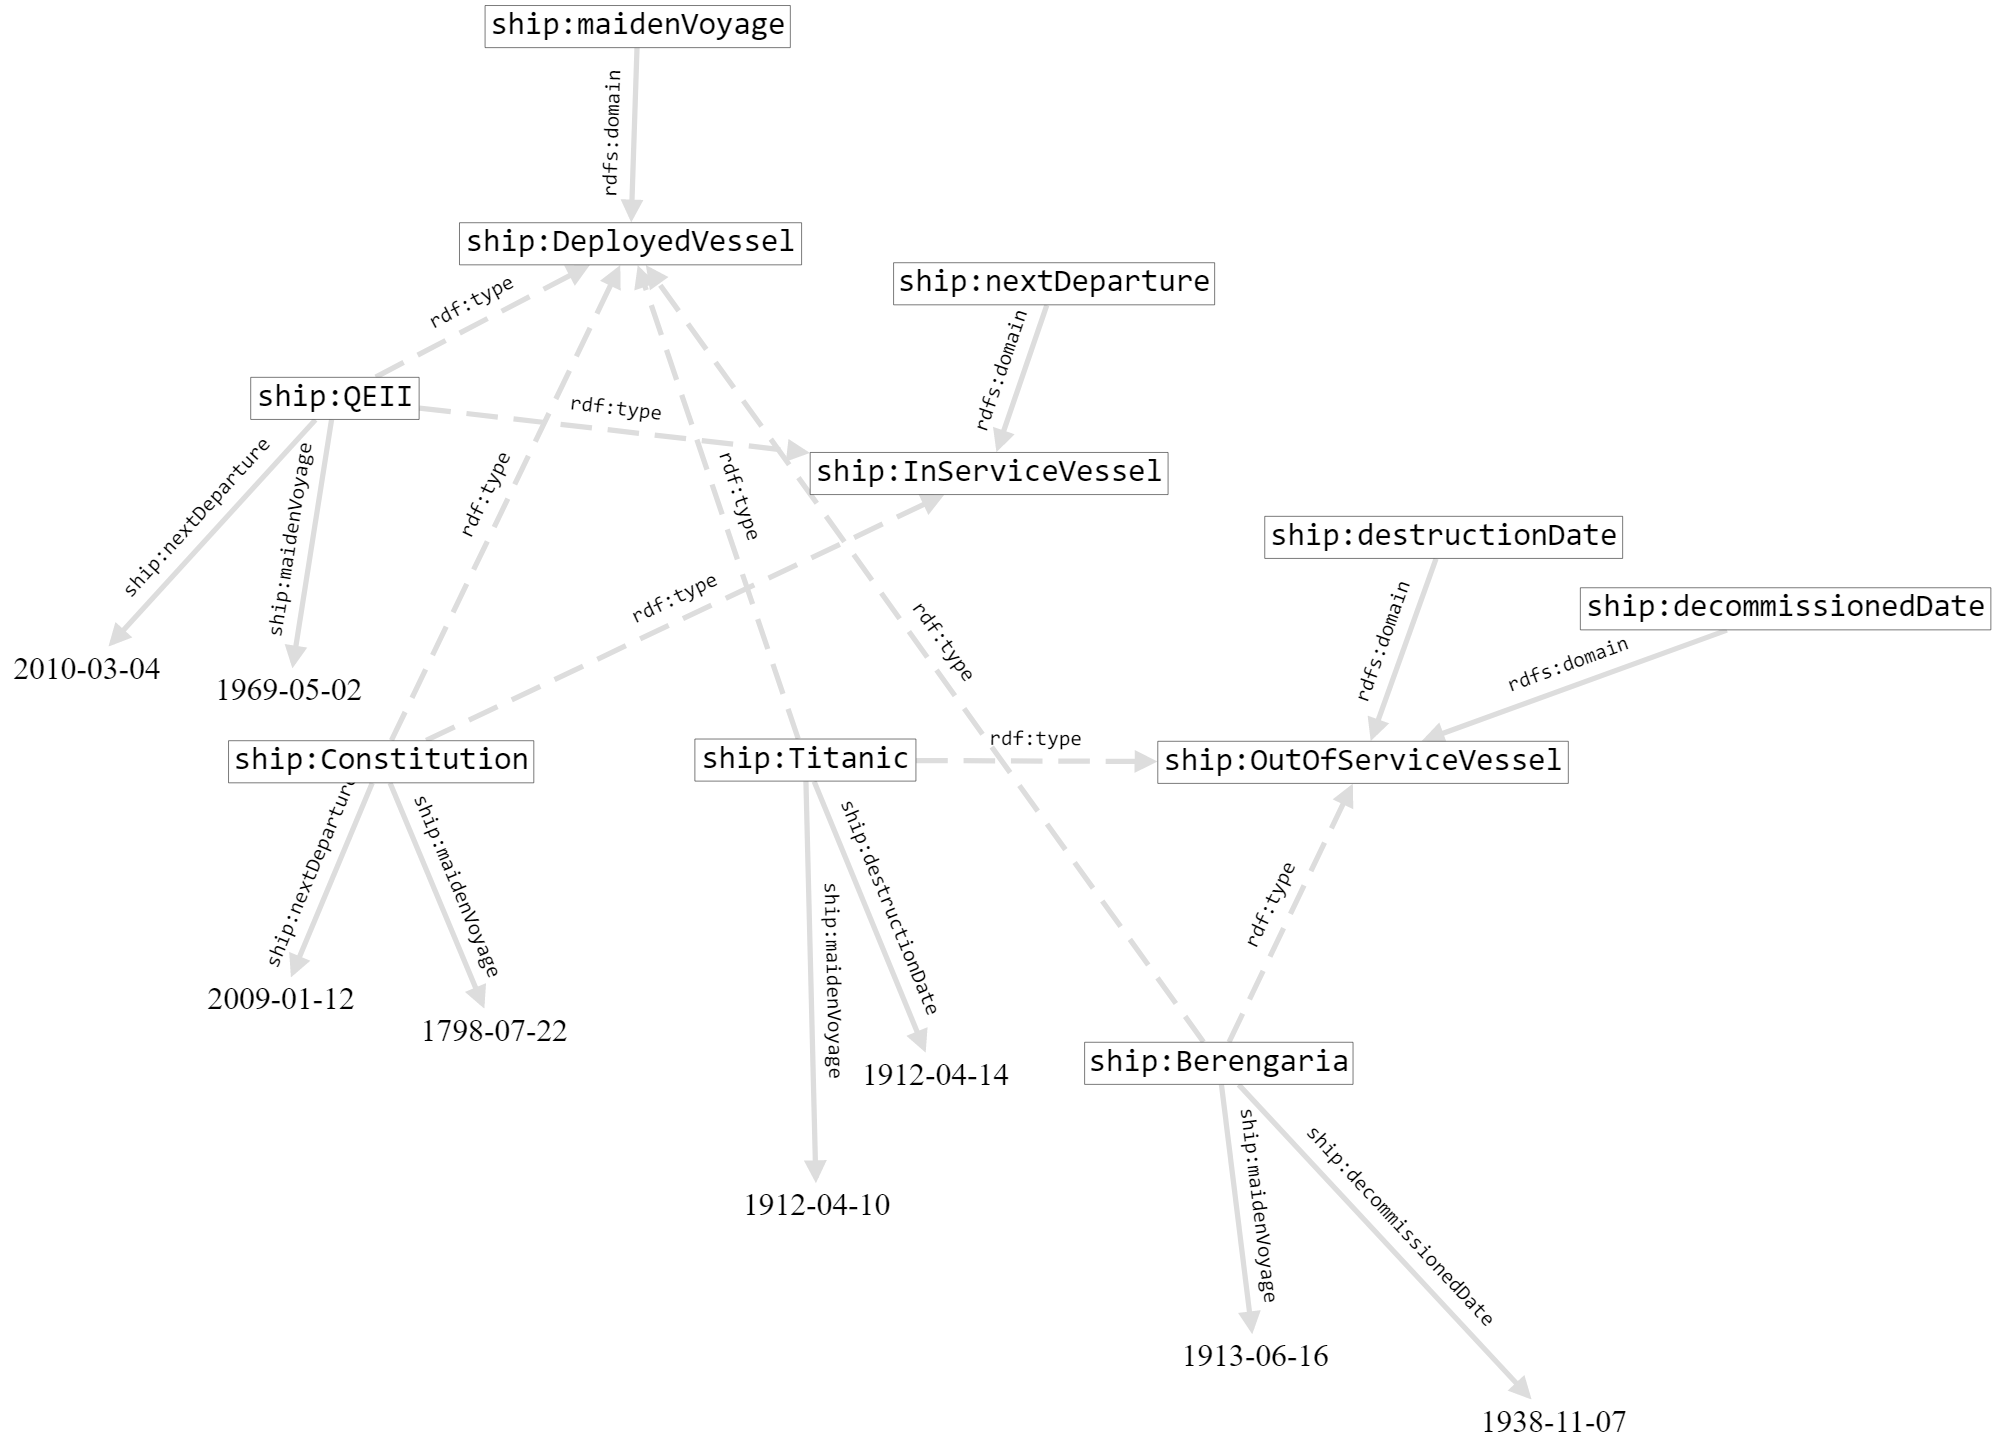
\includegraphics[width=5in]{SWWOv3/media/ch8/figure8-3.png}
\caption{Inferring classes of vessels from the information known about them.}
\label{fig:ch8.3}
\end{figure}


From the information in Table~\ref{tab:ch8.1}, we can infer that all of Johnson,
Warwick, Smith, and Preble are members of the class \texttt{ship:Captain}. These
inferences, as well as the triples that led to them, can be seen in
Figure~\ref{fig:ch8.4}.

\begin{figure}
\centering
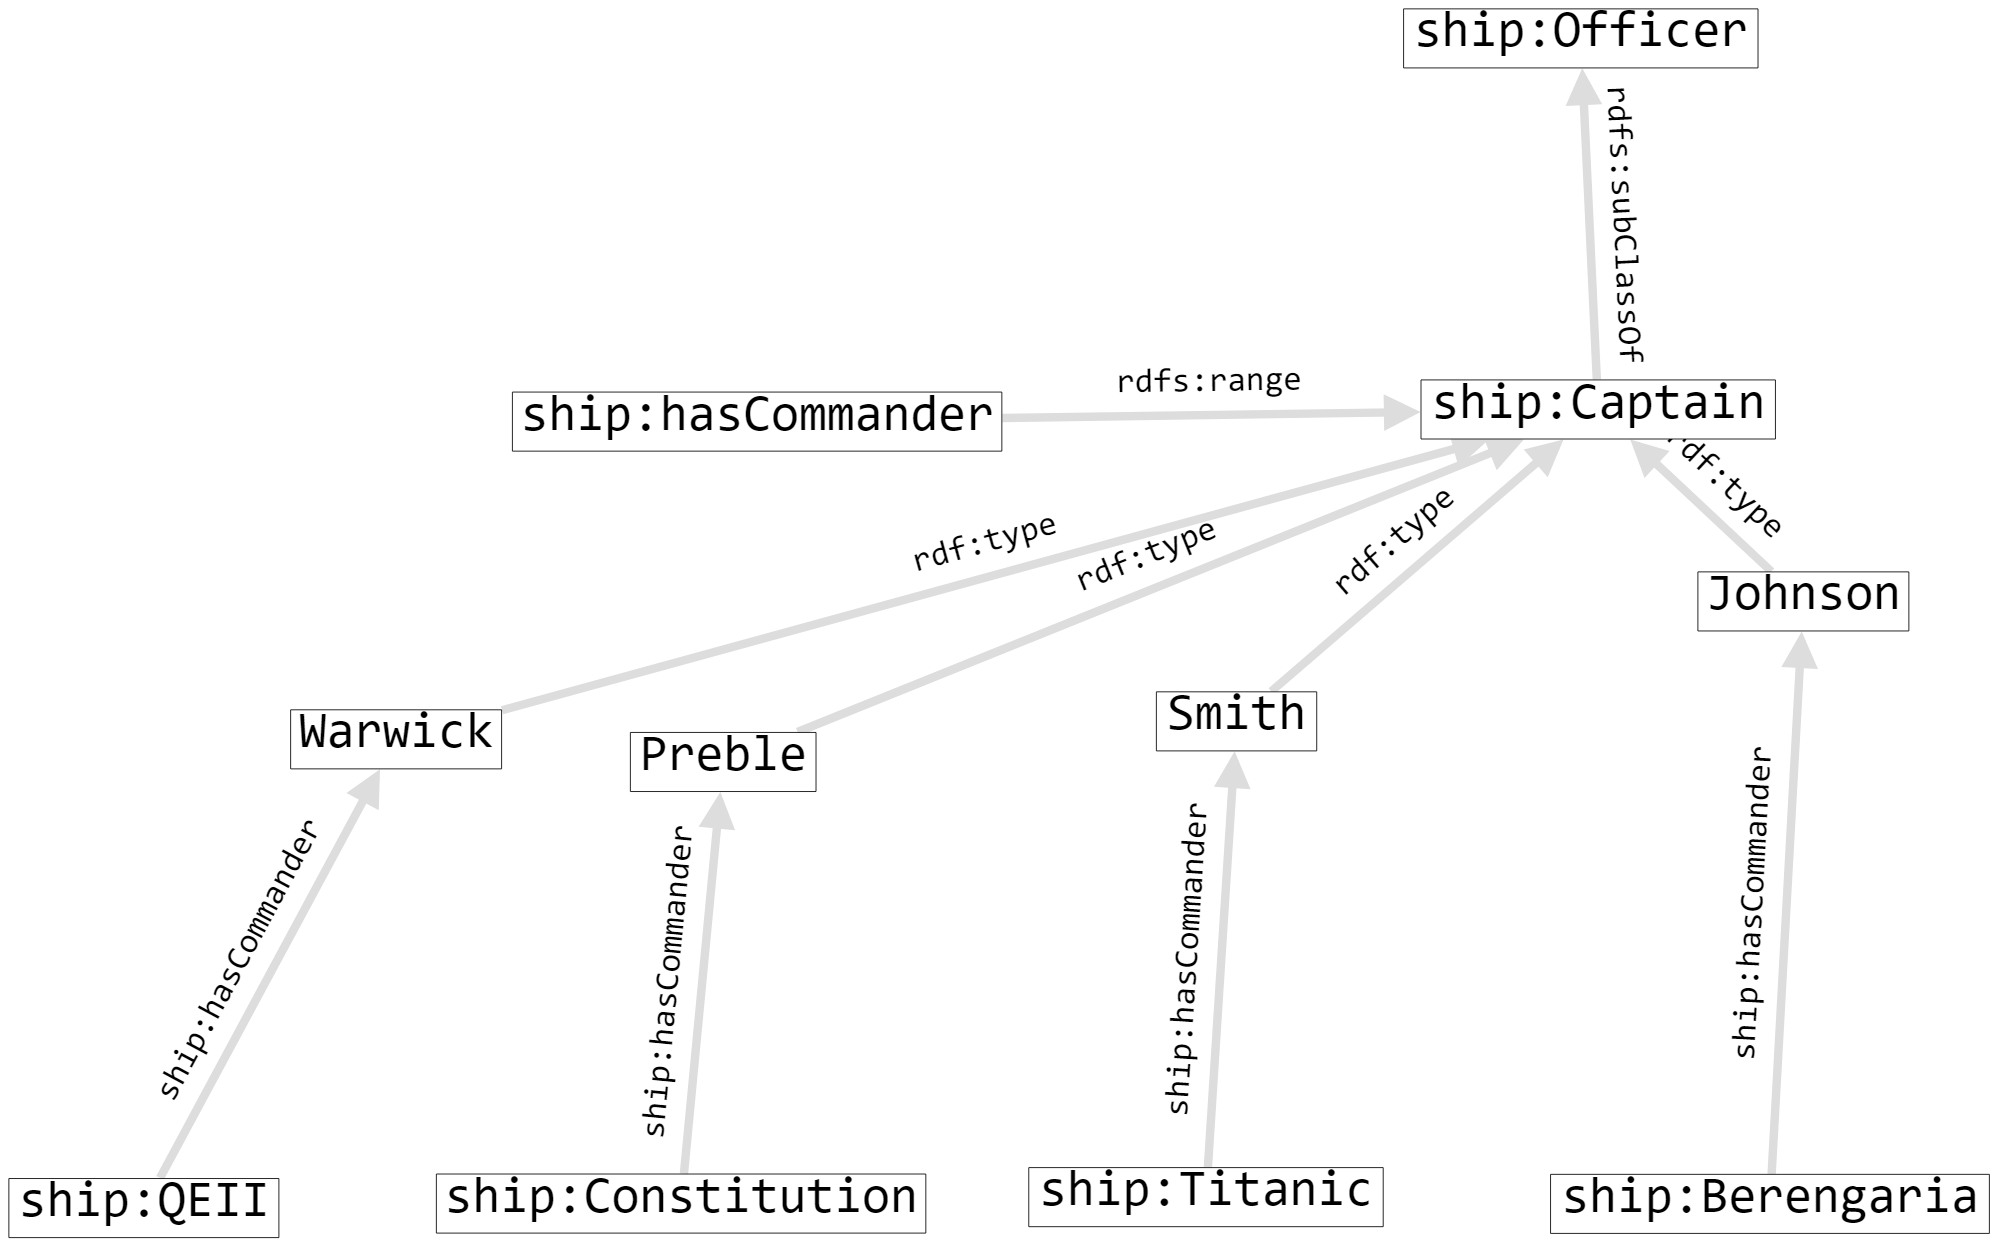
\includegraphics[width=5in]{SWWOv3/media/ch8/figure8-4.png}
\caption{Inferring that the commanders of the ships have rank "Captain"}
\label{fig:ch8.4}
\end{figure}


\end{challenge}

\subsection{Filtering undefined data}

A related challenge is to sort out individuals based on the information
that is defined for them. The set of individuals for which a particular
value is defined should be made available for future processing; those
for which it is undefined should not be processed.

\begin{challenge}{Filtering on undefined data}
\label{chal:12}

In the preceding example, the set of vessels for which \texttt{nextDeparture} is
defined could be used as input to a scheduling system that plans group
tours. Ships for which no \texttt{nextDeparture} is known should not be
considered.

\solution

It is easy to define the set of vessels that have \texttt{nextDeparture}
specified by using \texttt{rdfs:domain}. First, define a class of
\texttt{DepartingVessels} that will have these vessels as its members. Then
define this to be the domain of \texttt{nextDeparture}:

\begin{lstlisting}
ship:DepartingVessel rdf:type rdfs:Class .
ship:nextDeparture rdfs:domain ship:DepartingVessel .
\end{lstlisting}

From Table~\ref{tab:ch8.1}, only the Constitution and the QEII are members of the
class 
\texttt{ship:DepartingVessels} and can be used by a scheduling program (see
Figure~\ref{fig:ch8.5}).
\end{challenge}

\subsection{RDFS and knowledge discovery}

The use of \texttt{rdfs:domain} and \texttt{rdfs:range} differs dramatically from similar
notions in other modeling paradigms. Because of the inference-based
semantics of RDFS (and OWL), domains and ranges are not used to validate
information (as is the case, for example, in OO modeling and XML) but
instead are used to determine new information based on old information.
We have just seen how this unique aspect of \texttt{rdfs:domain} and \texttt{rdfs:range}
supports particular uses of filtering and classifying information.

These definitions are among the most difficult for beginning Semantic
Web modelers to come to terms with. It is common for beginning modelers
to find these tools clumsy and difficult to use. This difficulty can be
ameliorated to some extent by understanding that RDFS in general, and
domain and range in particular, are best understood as tools for
knowledge discovery rather than knowledge description. On the Semantic
Web, we don't know in advance how information from somewhere else
on the Web should be interpreted in a new context. The RDFS definitions
of domain and range
allow us to discover new things about our data based on its use.


\begin{figure}
\centering
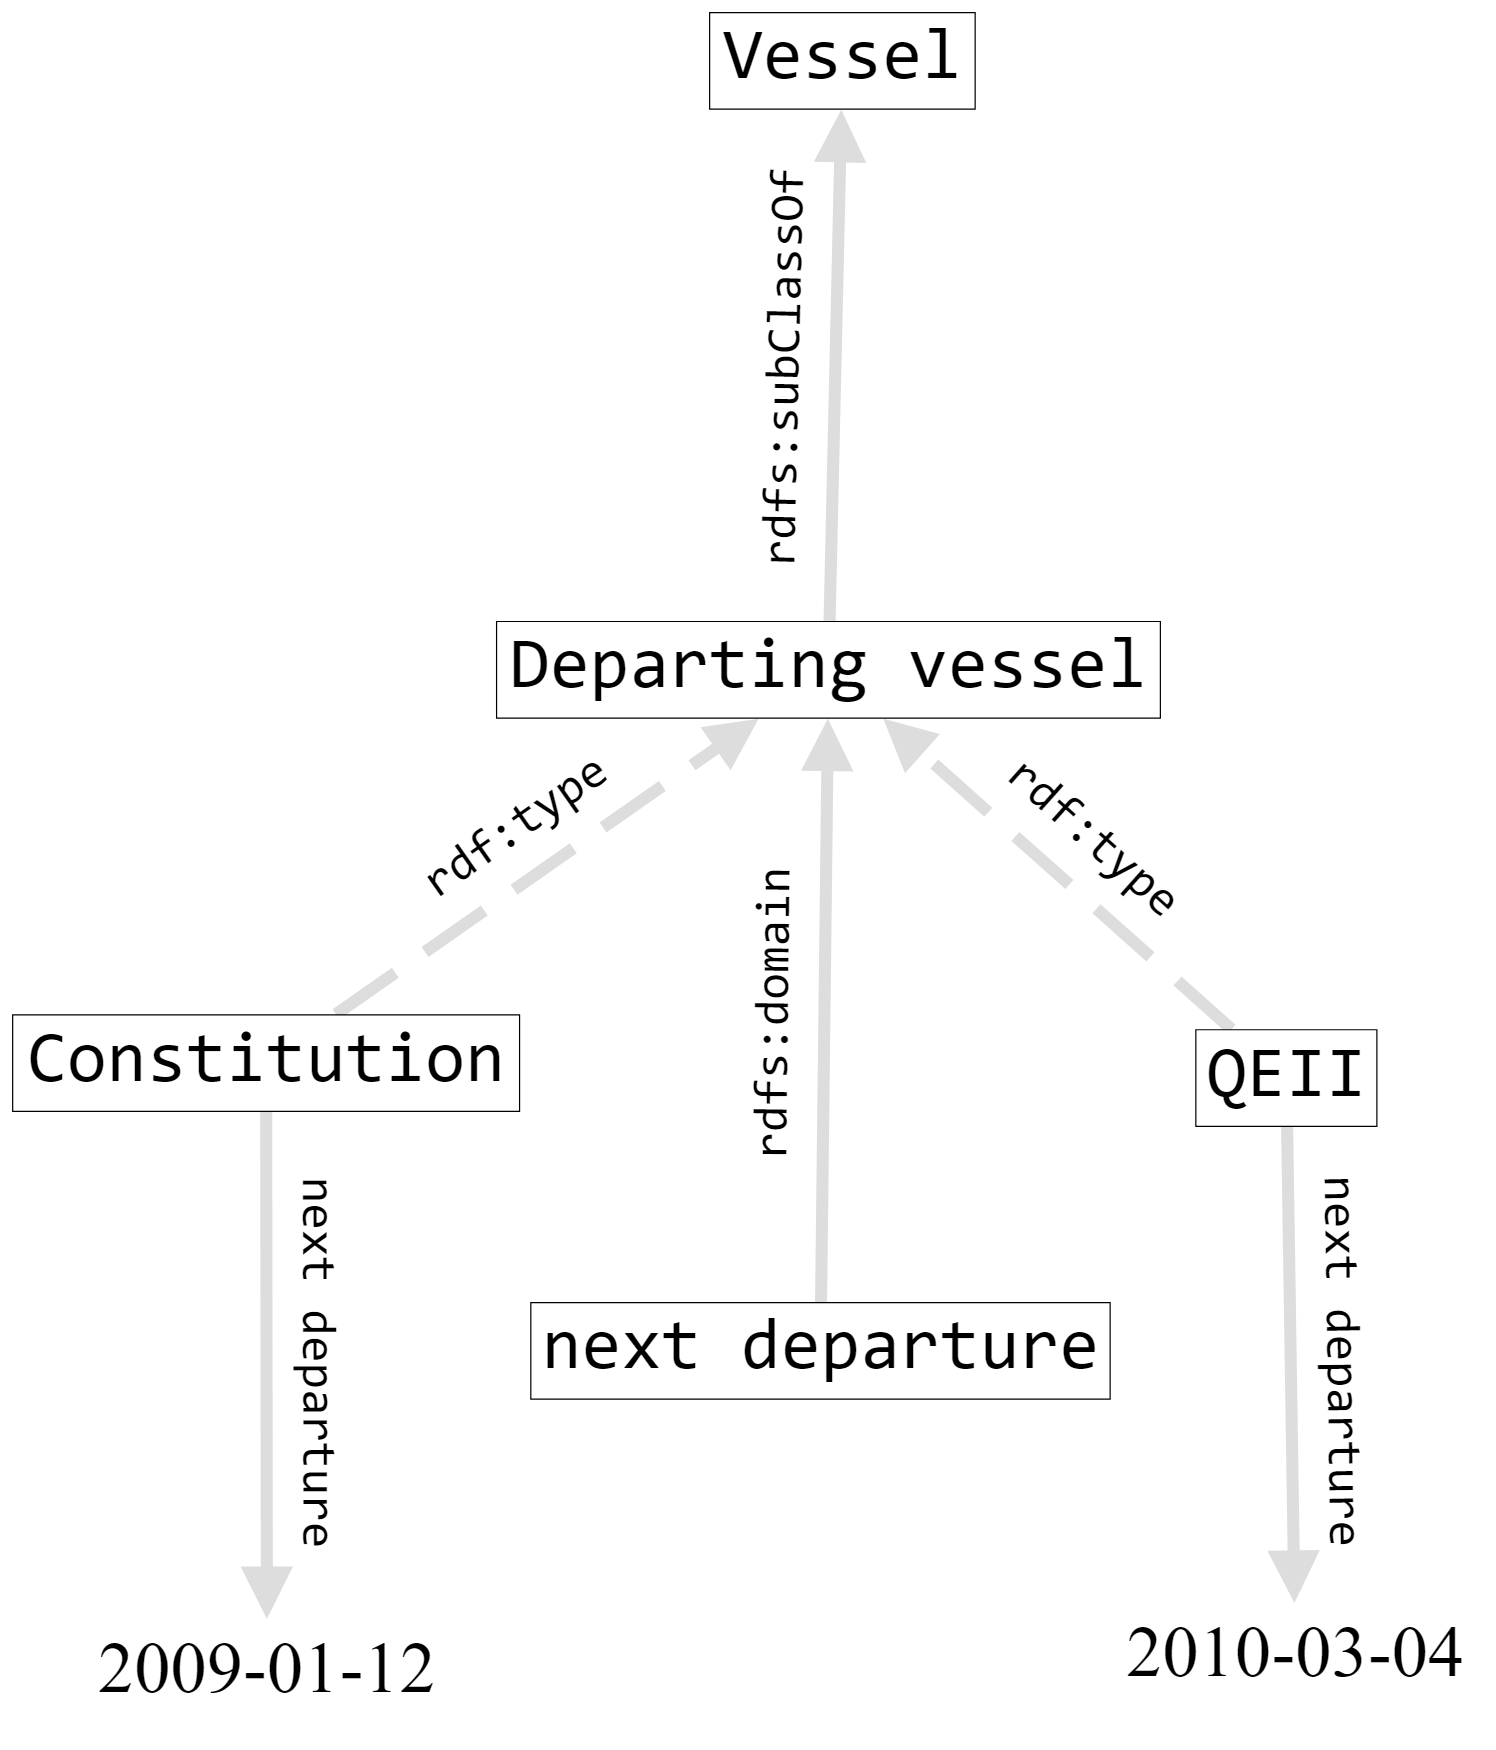
\includegraphics[width=5in]{SWWOv3/media/ch8/figure8-5.png}
\caption{\label{fig:ch8.5}Ships with a nextDeparture specified are DepartingVessels.}
\end{figure}





What does this mean for the skillful use of domain and range in RDFS?
They are not to be used lightly---that is, merely as a way to bundle
together several properties around a class. Filtering results such as
those shown in these challenge problems are the result of the use of
domain and range. Proper use of domain and range must take these results
into account. Recommended use of domain and range goes one step further;
its use is in one of these patterns, where some particular knowledge
filtering or discovery pattern is intended. When used in this way (e.g.,
using domain to describe which of the ships are departing), it is
guaranteed that the meaning of domain and range will be appropriate even
in a web setting.

\section{Modeling with Domains and Ranges}

Although RDFS has considerable applicability in data amalgamation and
the simplicity of its small number of axioms makes it compact and easy
to implement, there are some confusions that arise even in very simple
modeling situations when using RDFS.

\subsection{Multiple domains/ranges}
\label{multidomain}
In our shipping example, we had two definitions for the \texttt{nextDeparture}
domain:

\begin{lstlisting}
ship:nextDeparture rdfs:domain DepartingVessel .
ship:nextDeparture rdfs:domain InServiceVessel .
\end{lstlisting}

What is the interpretation of these two statements? Is the \texttt{nextDeparture}
domain \texttt{DepartingVessel}, \texttt{InServiceVessel}, or both? What does this sort of
construction mean?

The right way to understand what a statement or set of statements means
in RDFS is to understand what inferences can be drawn from them. Let's
consider the case of the QEII, for which we have the following asserted
triples:

\begin{lstlisting}
ship:QEII ship:maidenVoyage "May 2, 1969" .
ship:QEII ship:nextDeparture "Mar 4, 2010" .
ship:QEII ship:hasCommander Warwick .
\end{lstlisting}

The rules of inference for \texttt{rdfs:domain} allow us to draw the following
conclusions:

\begin{lstlisting}
ship:QEII rdf:type ship:DepartingVessel.
ship:QEII rdf:type ship:InServiceVessel.
\end{lstlisting}

Each of these conclusions is drawn from the definition of \texttt{rdfs:domain},
as applied, respectively, to each of the domain declarations just given.
This behavior is not a result of a discussion of ``what will happen when
there are multiple domain statements?'' but rather a simple logical
conclusion based on the definition of \texttt{rdfs:domain}.

How can we interpret these results? Any vessel for which a \texttt{nextDeparture}
is specified will be
inferred to be a member (i.e., \texttt{rdf:type}) of both \texttt{DepartingVessel} and
\texttt{InServiceVessel} classes. Effectively, any such vessel will be inferred
to be in the intersection of the two classes specified in the domain
statements. This is something that many people find counterintuitive,
even though it is ``correct'' in RDFS.

In object-oriented modeling, when one asserts that a property (or field,
or variable, or slot) is associated with a class (as is done by
\texttt{rdfs:domain}), the intuition is that ``it is now permissible to use this
property to describe members of this class.'' If there are two such
statements, then the intuitive interpretation is that ``it is now
permissible to use this property with members of either of these
classes.'' Effectively, multiple domain declarations are interpreted in
the sense of set union: You may now use this property to describe any
item in the union of the two specified domains. For someone coming in
with this sort of expectation, the intersection behavior of RDFS can be
something of a surprise.

This interaction makes it necessary to exercise some care when modeling
information with the expectation that it will be merged with other
information. Let's suppose we have another modeling context in which a
company is managing a team of traveling salespeople. Each salesperson
has a schedule of business trips. Some of the triples that define this
model are as follows:

\begin{lstlisting}
sales:SalesPerson rdfs:subClassOf foaf:Person.
sales:sells rdfs:domain sales:SalesPerson.
sales:sells rdfs:range sales:ProductLine.
sales:nextDeparture rdfs:domain sales:SalesPerson.
\end{lstlisting}

That is, we have a sales force that covers certain \texttt{ProductLines}; each
member travels on a regular basis, and it is useful for us to track the
date of the next departure of any particular \texttt{SalesPerson}.

Suppose we were to merge the information for our sales force management
with the schedules of
the ocean liners. This merge becomes interesting if we map some of the
items in one model to items
in another. An obvious candidate for such a mapping is between
\texttt{sales:nextDeparture} and \texttt{ship:nextDeparture}. Both refer to dates, and the
intuition is that they specify the next departure date of something or
someone. So a simple connection to make between the two models would be
to link these two properties, such as the following:

\begin{lstlisting}
sales:nextDeparture rdfs:subPropertyOf ship:nextDeparture.
ship:nextDeparture rdfs:subPropertyOf sales:nextDeparture.
\end{lstlisting}

using the mutual \texttt{subPropertyOf} pattern. The intuition here is that the
two uses of
\texttt{nextDeparture}, one for ships and the other for sales, are in fact the
same.

But wait! Let's see what inferences are drawn from this merger. Suppose
we have a triple that describes a member of the sales force:

\begin{lstlisting}
sales:Johannes sales:nextDeparture "May 31, 2008".
\end{lstlisting}

and we already have the triple about the QEII:

\begin{lstlisting}
ship:QEII ship:nextDeparture "Mar 4, 2010".
\end{lstlisting}

What inferences can we draw from these two triples? Using
\texttt{rdfs:subPropertyOf} inferences first, then \texttt{rdfs:domain} inferences, and
finally using the \texttt{rdfs:subClassO}f triple with \texttt{foaf:Person}, we get the
following inferred triples:

\begin{lstlisting}
* sales:Johannes ship:nextDeparture "May 31, 2008".
* ship:QEII sales:nextDeparture "Mar 4, 2010".
* sales:Johannes rdf:type ship:DepartingVessel.
* ship:QEII rdf:type sales:SalesPerson.
* ship:QEII rdf:type foaf:Person.
\end{lstlisting}


These inferences start off innocently enough, but they become more and
more counterintuitive as they go on, and eventually (when the QEII is
classified as a \texttt{foaf:Person}) become completely outrageous (or perhaps
dangerously misleading, especially given that the Monarch herself might
actually be a \texttt{foaf:Person}, causing the inferences to confuse the Monarch
with the ship named after her). The asserted triples, and the inferences
that can be drawn from them, are shown in Figure~\ref{fig:ch8.6}.

It is easy to lay blame for this unfortunate behavior at the feet of the
definition of \texttt{rdfs:domain}, but to do so would throw out the baby with
the bathwater. The real issue in this example is that we have made a
modeling error. The error resulted from the overzealous urge to jump to
the conclusion that two properties should be mapped so closely to each
other. The ramifications of using \texttt{subPropertyOf} (or any other RDFS
construct) can be subtle and far-reaching.

In particular, when each of these models stated its respective domain
and range statements about \texttt{sales:nextDeparture} and \texttt{ship:nextDeparture},
respectively, it was saying, ``Whenever you see any individual described
by \texttt{sales:nextDeparture} (resp. \texttt{ship:nextDeparture}), that individual is
known to be of type \texttt{sales:SalesPerson} (resp. \texttt{ship:DepartingVessel}).''
This is quite a strong statement, and it should be treated as such. In
particular, it would be surprising if two properties defined so
specifically would not have extreme ramifications when merged.

\begin{figure}
\centering
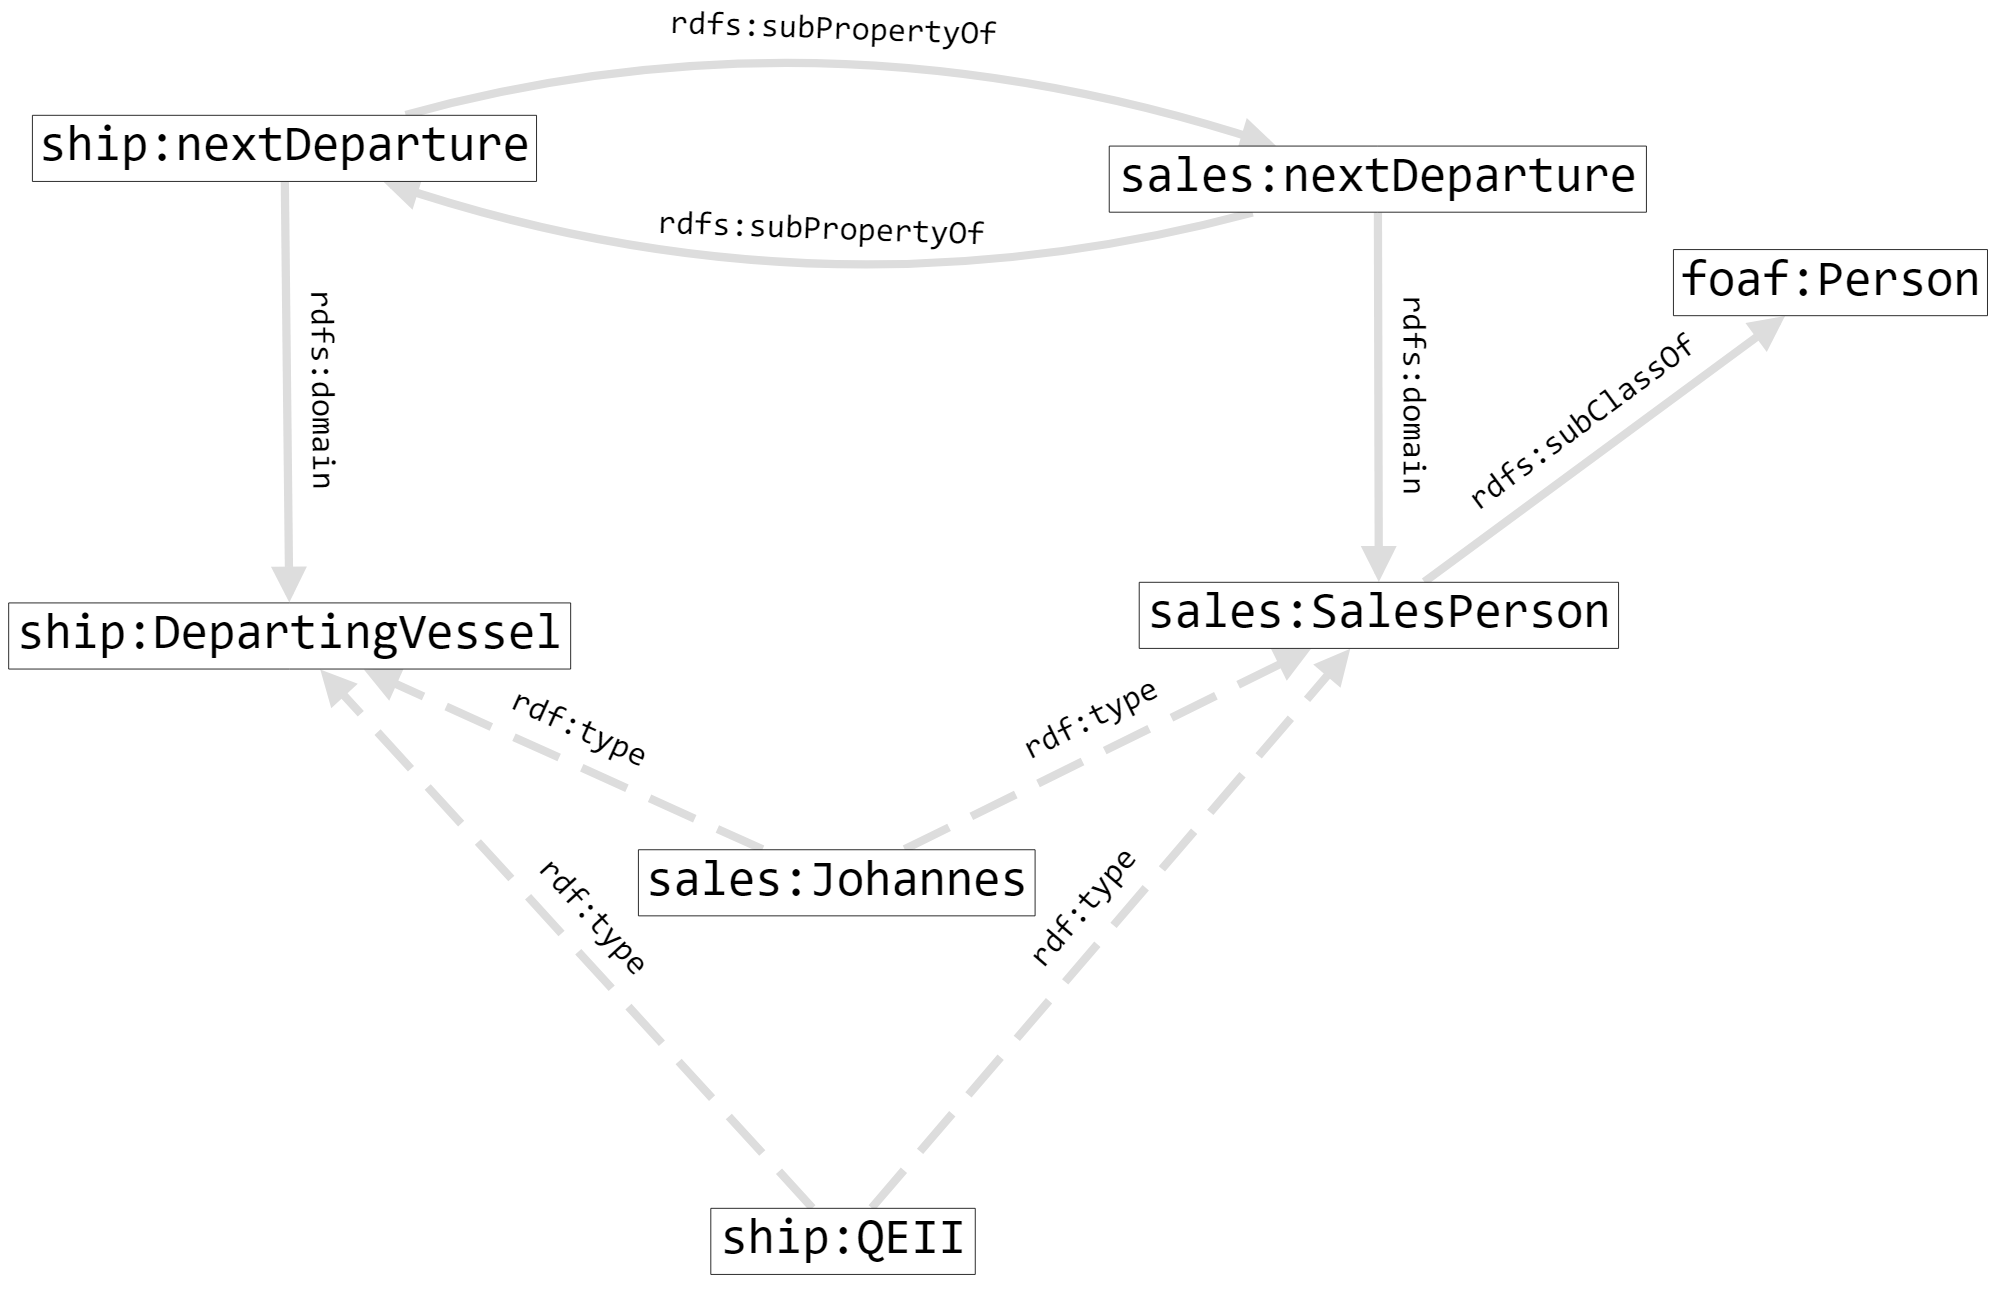
\includegraphics[width=5in]{SWWOv3/media/ch8/figure8-6.png}
\caption{Inferences resulting from merging two notions of nextDeparture.}
\label{fig:ch8.6}
\end{figure}



So what is the solution? Should we refrain from merging properties? This
is hardly a solution in the spirit of the Semantic Web. Should we avoid
making strong statements about properties? This will not help us to make
useful models. Should we change the RDFS standard so we can't make these
statements? This is a bit extreme, but as we shall see, OWL does provide
some more subtle constructs for property definitions that allow for
finer-grained modeling. Rather, the solution lies in understanding the
source of the modeling error that is at the heart of this example: We
should refrain from merging things, like the two notions of
\texttt{nextDeparture}, whose meanings have important differences.

Using the idioms and patterns of RDFS shown in this chapter, there are
more things we can do, depending on our motivation for the merger. In
particular, we can still merge these two properties but without making
such a strong statement about their equivalence.

If, for instance, we just want to merge the two notions of \texttt{nextDeparture}
to drive a calendar application that shows all the departure dates for
the sales force and the ocean liner fleet, then what we really want is a
single property that will provide us the information we need (as we did
in the property union pattern). Rather than mapping the properties from
one domain to another, instead we map both properties to a third,
domain-neutral property, thus:

\begin{lstlisting}
ship:nextDeparture rdfs:subPropertyOf cal:nextDeparture .
sales:nextDeparture rdfs:subPropertyOf cal:nextDeparture .
\end{lstlisting}

Notice that the amalgamating property \texttt{cal:nextDeparture} doesn't need any
domain information at all. After all, we don't need to make any
(further) inferences about the types of the entities that it is used to
describe. Now we can infer that

\begin{lstlisting}
* sales:Johannes cal:nextDeparture "May 31, 2008" .
* ship:QEII cal:nextDeparture "Mar 4, 2010" .
\end{lstlisting}

A single calendar display, sorted by the property \texttt{cal:nextDeparture},
will show these two dates, but no further inference can be made. In
particular, no inferences will be made about considering the QEII as a
member of the sales force or Johannes as a sailing vessel.

This behavior of RDFS is not an idiosyncrasy of how it was defined, it is
a direct result of the fact that on the Semantic Web, we are representing distributed
data, and that includes distributed metadata.  Each stakeholder is telling us 
something about one of their properties (in this example, \texttt{ship:nextDeparture} and
\texttt{sales:nextDeparture}).  We need to be able to draw conclusions from 
each of these things in their own context.  But when we combine them (as 
we did, when we asserted that they were sub properties of one another), now we 
have to accept both definitions together.  This isn't an arbitrary decision on 
the part of the RDF design; it is simply a ramification of treating the statements
from each contributor equally.  If we believe what the Sales domain says, and we believe
what the Ship domain says, and if we believe our mapping, then the domain must 
be the intersection of the stated domains.   When we resolve this situation (e.g., by
making a new property, \texttt{cal:nextDeparture} that encompasses both of these properties
we are being specific about the relationship between them.  This is what we have to
do, to be able to use both data sources together. 

This is the art of modeling in the Semantic Web; to state specifically and in sufficient 
detail how two or more data sets (or metadata sets) are related.  The inference model
behind languages like RDFS and OWL provide the precision we need to build this kind of model. 



\section{Nonmodeling Properties in RDFS}

In addition to the properties described so far, RDFS also provides a
handful of properties that have no defined inference semantics---that
is, there are no inferences that derive from them. We already saw one
example of such a property, \texttt{rdfs:label}. No inferences are drawn from
\texttt{rdfs:label}, so in that sense it has no semantics. Nevertheless, it does
by convention have an operational semantics in that it describes the
ways in which display agents interact with the model.

\subsection{Cross-referencing files: rdfs:seeAlso}

Every resource in a Semantic Web model is specified by a URI that can
also be dereferenced and used as a URL. In the case where this URL
resolves to a real document, this provides a place where defining
information about a resource can be stored.

In some contexts, it is useful to include some supplementary information
about a resource for its use in a certain context. This is usually meant
to be other documents that might help explain the entity---for example,
we might include a pointer to a Wikipedia entry, or a pointer to related
data (e.g., if the resource corresponds to a table from a database, the
supplementary information could be the other tables from the same
database) or even to another RDF or RDFS file that contains linked
information. For such cases, \texttt{rdfs:seeAlso} provides a way to specify the
web location of this supplementary information (i.e. it should be a URI,
not a human-readable property). \texttt{rdfs:seeAlso} has no formal semantics, so
the precise behavior of any processor when it encounters \texttt{rdfs:seeAlso} is
not specified. A common behavior of tools that encounter \texttt{rdfs:seeAlso}
links is to expose those links in a browser or application interface
through which the RDFS document is being used.

\subsection{Organizing vocabularies: rdfs:isDefinedBy}

Just as \texttt{rdfs:seeAlso} can provide supplementary information about a
resource, \texttt{rdfs:isDefinedBy} provides a link to the primary source of
information about a resource. This allows modelers to specify where the
definitional description of a resource can be found. \texttt{rdfs:isDefinedBy} is
defined in RDF to be a \texttt{rdfs:subPropertyOf} of \texttt{rdfs:seeAlso}.

\subsection{Model documentation: rdfs:comment}

Just as in any computer language (modeling languages, markup languages,
or programming languages), sometimes it is helpful if a document author
can leave natural language comments about a model for future readers to
see. Since RDFS is implemented entirely in RDF, the comment feature is
also implemented in RDF. To make a comment on some part of a model,
simply assert a triple using the property \texttt{rdfs:comment} as a predicate.
A good practice is also to indicate the natural language used to support 
internationalization of data, applications and interfaces, as follows:

\begin{lstlisting}
sales:nextDeparture rdfs:comment
   "This indicates the next planned departure date for a salesperson."@en ,
   "Ceci indique la prochaine date de d(*@\'e@*)part pr(*@\'e@*)vue pour un vendeur."@fr .
\end{lstlisting}

\section{SUMMARY}

RDFS is the schema language for RDF; it describes constructs for types
of objects (Classes), relating types to one another (subClasses),
properties that describe objects (Properties), and relationships between
them (subProperty). The Class system in RDFS includes a simple and
elegant notion of inheritance, based on set inclusion; one class is a
subclass of another means that instances of the one are also instances
of the other.

The RDFS language benefits from the distributed nature of RDF and all
its tools by being expressed in RDF itself. All schema information
(classes, subclasses, subproperties, domain, range, etc.) is expressed
in RDF triples. In particular, this makes schema information, as well as
data, subject to the AAA slogan: Anyone can say Anything about Any
topic---even about the schema.

The semantics of RDFS is expressed through the mechanism of inferencing;
that is, the meaning of any construct in RDFS is given by the inferences
that can be inferred from it. For example, it is this simple but
powerful mechanism for specifying semantics that allows for the short
and elegant definition of subclass and subproperty.

RDFS also includes the constructs \texttt{rdfs:domain} and \texttt{rdfs:range} to describe
the relationship between properties and classes. The meanings of these
constructs are given by very simple rules, but these rules have subtle
and far-reaching impact. The rules may be simple, but the statements are
powerful.

Even with its small set of constructs and simple rules, RDFS allows for
the resolution of a wide variety of integration issues. Whenever you
might think of doing a global find-and-replace in a set of structured
data, consider using \texttt{rdfs:subPropertyOf} or \texttt{rdfs:subClassOf} instead. It
may seem trivial to say that one should merge only entities from
multiple sources that don't have important differences. Using the
inference mechanism of RDFS, we can determine just what happens when we
do merge things and judge whether the results are desirable or
dangerous. Although RDFS does not provide logical primitives like union
and intersection, it is often possible to achieve desired inferences by
using specific patterns of \texttt{subClassOf} and \texttt{subPropertyOf}. RDFS provides a
framework through which information can flow; we can think of \texttt{subClassOf}
and \texttt{subPropertyOf} as the IF/ THEN facility of semantic modeling. This
utility persists even when we move on to modeling in OWL. In fact, using
\texttt{subClassOf} in this way provides a cornerstone of OWL modeling.

When used in careful combination, the constructs of RDFS are
particularly effective at defining

how differently structured information can be used together in a uniform
way.

\subsection{Fundamental concepts}

The following fundamental concepts were introduced in this chapter.

rdfs:subClassOf---Relation between classes, that the members of one
class are included in the members of the other.

rdfs:subPropertyOf---Relation between properties, that the pairs related
by one property are included in the other.

rdfs:domain and rdfs:range---Description of a property that determines
class membership
of individuals related by that property.

Logical operations (Union, Intersection, etc.) in RDFS---RDFS constructs
can be used to simulate certain logical combinations of sets and
properties.

\chapter{RDFS-Plus}
\label{ch9}

RDFS provides a very limited set of inference capabilities that, as we
have seen, have considerable utility in a Semantic Web setting for
merging information from multiple sources. In this chapter, we take the
first step toward the Web Ontology Language, OWL, in which more
elaborate constraints on how information is to be merged can be
specified. We have selected a particular set of OWL constructs to
present at this stage. This set was selected to satisfy a number of
goals:

\begin{itemize}
\item Pedagogically, these constructs constitute a gentle addition to the
constructs that are already familiar from RDFS, increasing the power of
the language without making a large conceptual leap from RDFS.

\item Practically, we have found that this set of OWL constructs has
considerable utility in the
information integration projects we have done. In fact, it is much
easier to find and describe case studies using RDFS plus this set of OWL
constructs than it is to find case studies that use RDFS by itself.

\item Computationally, this subset of OWL can be implemented using a wide
variety of inferencing technologies, lessening the dependency between
the Semantic Web and any particular technology.
\end{itemize}

For these reasons, we feel that this particular subset will have value
beyond the pedagogical value in this book. We call this subset of OWL
\emph{RDFS-Plus}, because we have seen a trend among vendors of Semantic Web tools
and Web applications designers for determining a subset of OWL that is
at the same time useful and can be implemented quickly. We have
identified this particular subset via an informal poll of cutting-edge
vendors, and from our own experience with early adopters of Semantic Web
technology.

Just as was the case for RDFS, RDFS-Plus is expressed entirely in RDF.
The only distinction is
that there are a number of resources, all in the namespace \texttt{owl:}. The
meaning of these resources is specified, as before, by the rules that
govern the inferences that can be made from them. As we did for RDFS, we
will specify the rules that govern the inferences using SPARQL CONSTRUCT
queries.

In the case of RDFS, we saw how the actions of an inference engine could
be used to combine various features of the schema language in novel
ways. This trend will continue for RDFS-Plus, but as you might expect,
the more constructs we have to begin with, the more opportunity we have
for useful and novel combinations.

\section{Inverse}

The names of many of the OWL constructs come from corresponding names in
mathematics. Despite their mathematical names, they also have a more
common, everyday interpretation. The idea \texttt{owl:inverseOf} is a prime
example; if a relationship---say, \texttt{hasParent}---is interesting enough to
mention in a model, then it's a good bet that another
relationship---say, \texttt{hasChild}---is also interesting. Because of the
evocative names \texttt{hasParent} and \texttt{hasChild}, you can guess the relationship
between them, but of course the computer can't. The OWL construct
\texttt{owl:inverseOf} makes the relationship between \texttt{hasParent} and \texttt{hasChild}
explicit, and describes precisely what it means.

In mathematics, the inverse of a function $f$ (usually written as $f^{-1}$) is
the function that satisfies the
property that if $f(x) = y$, then $f^-1(y) = x$. Similarly in OWL, the
inverse of a property is another property that reverses its direction.  This should not be confused with 
a semantic \textit{opposite};  you could imagine a model that describes two 
properties - \texttt{hasFriend} and \texttt{hasEnemy}.  These might be considered 'opposites', since 
by definition, a friend can't be an enemy and vice versa, but they are not mathematical inverses, in fact, far from it;
if I am your friend, it does not imply that you are my enemy.  OWL does not have a way to formally indicate this sort of 
relationship between properties. 

To be specific, we look at the meaning of \texttt{owl:inverseOf}. In OWL, as in
RDFS, the meaning of any construct is given by the inferences that can
be drawn from it. We can express the rule for owl:inverseOf in SPARQL as
follows:

\begin{lstlisting}
CONSTRUCT {?y ?q ?x}
WHERE {?p owl:inverseOf ?q .
       ?x ?p ?y . }
\end{lstlisting}

In the examples in the book, we have already seen a number of
possibilities for inverses, though we haven't used them so far. In our
Shakespeare examples, we have the triples

\begin{lstlisting}
lit:Shakespeare lit:wrote lit:Macbeth .
lit:Macbeth lit:setIn geo:Scotland .
\end{lstlisting}

If, in addition to these triples, we also state some inverses, such as:

\begin{lstlisting}
lit:wrote owl:inverseOf lit:writtenBy .
lit:settingFor owl:inverseOf lit:setIn .
\end{lstlisting}

then we can infer that

\begin{lstlisting}
lit:Macbeth lit:writtenBy lit:Shakespeare .
geo:Scotland lit:settingFor lit:Macbeth .
\end{lstlisting}

Although the meaning of \texttt{owl:inverseOf} is not difficult to describe, what
is the utility of such a construct in a modeling language? After all,
the effect of inverseOf can be achieved just as easily by writing the
query differently. For instance, if we want to know all the plays that
are \texttt{setIn} Scotland, we can use the inverse property \texttt{settingFor} in our
query pattern, such as

\begin{lstlisting}
{ geo:Scotland lit:settingfor ?play . }
\end{lstlisting}

Because of the semantics of the inverse property, this will give us all
plays that were setIn
Scotland.

But we could have avoided the use of the inverse property and simply
written the query as

\begin{lstlisting}
{ ?play lit:setIn geo:Scotland . }
\end{lstlisting}

We get the same answers, and we don't need an extra construct in the
modeling language.

While this is true, \texttt{owl:inverseOf} nevertheless does have considerable
utility in modeling, based on how it can interact with other modeling
constructs. In the next two challenges, we'll see how some earlier
challenges can be extended using inverses.

\begin{challenge}{continued from \protect\ref{chal:2}: Using SPARQL to Transform Hierarchical Data}

In Chapter\ref{ch6} we saw a Challenge problem to use SPARQL to transform
hierarchical data. The original data was expressed using a variety of
properties like \texttt{hasSon}, \texttt{hasMother}, \texttt{hasDaughter}, and \texttt{hasFather}. The
response to the challenge involved a series of SPARQL queries to
transform e.g., \texttt{hasMother} into \texttt{hasParent}. The queries that accomplished
the transformations all had a very similar form, e.g.,

\begin{lstlisting}
CONSTRUCT {?s :hasParent ?o}
WHERE {?s :hasMother ?o}
\end{lstlisting}


The transformation that this query accomplishes can also be represented
in RDFS. This query says ``whenever a triple uses hasMother, infer a
similar triple with hasParent.'' This can be expressed in RDFS by
relating the two properties together with \texttt{subPropertyOf}, thus:

\begin{lstlisting}
:hasMother rdfs:subPropertyOf :hasParent .
\end{lstlisting}

When we combine this statement with the definition of \texttt{subPropertyOf}, we
see that we come to the same conclusions---from every triple that uses
hasMother we can infer a similar triple using hasParent.

Some of the queries included a bit of a twist on this pattern---for
example, one query rectified uses of
\texttt{hasSon} as follows:

\begin{lstlisting}
CONSTRUCT {?s :hasParent ?o}
WHERE {?o :hasSon ?s}
\end{lstlisting}



\begin{figure}
\centering
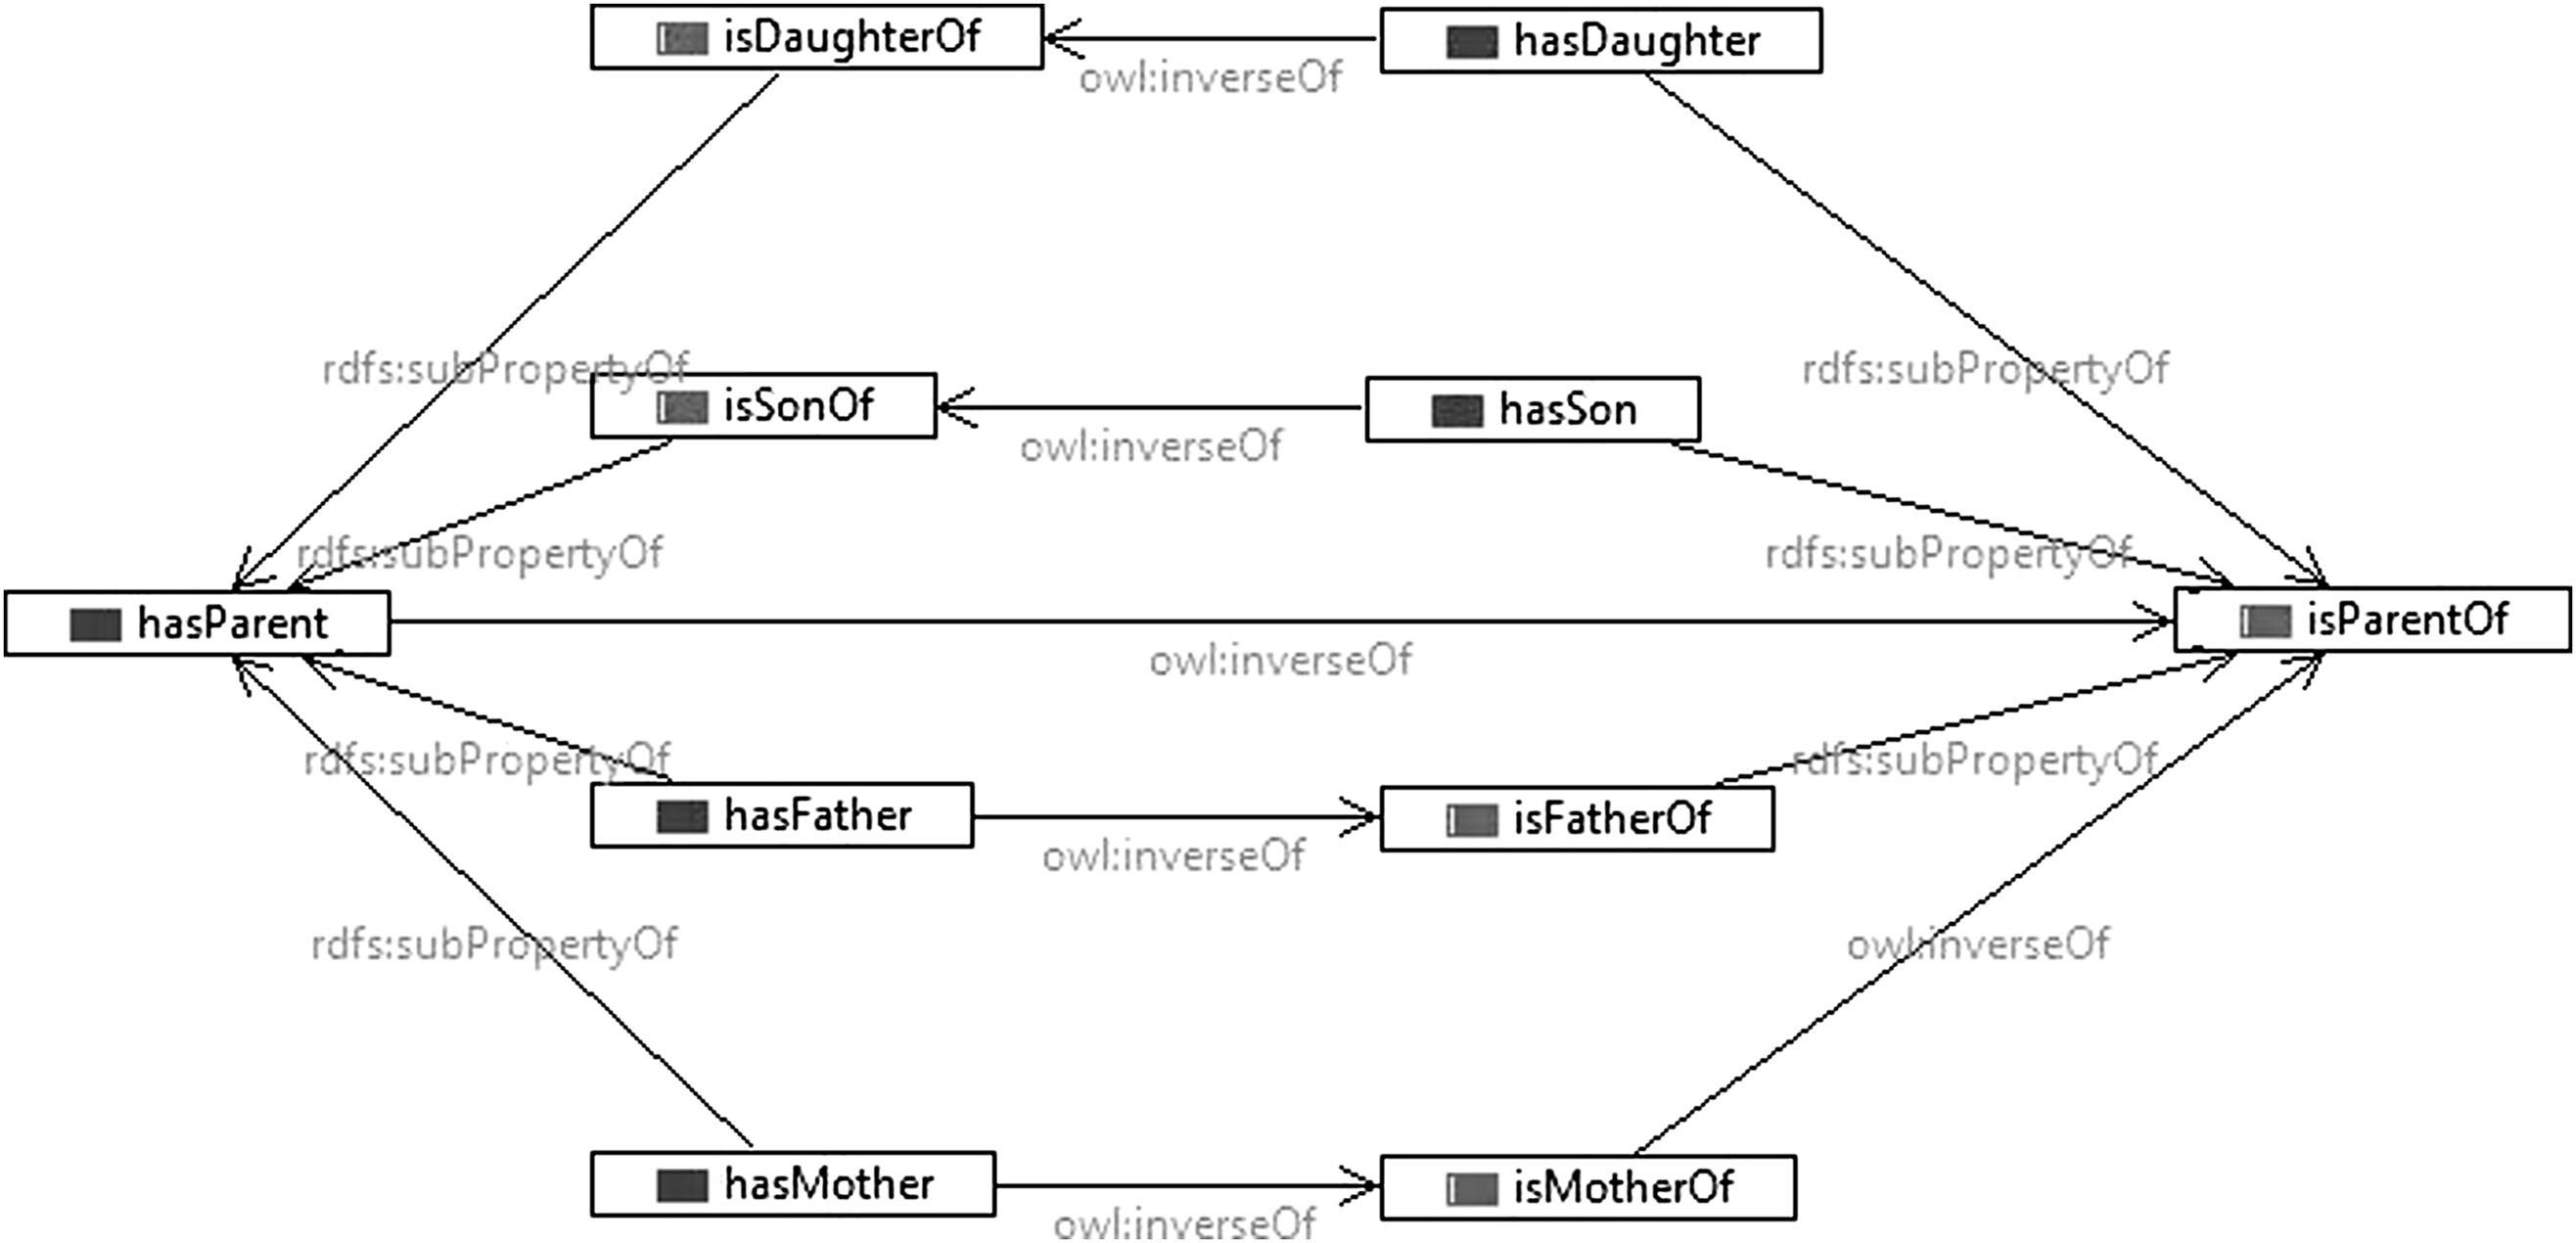
\includegraphics[width=5in]{media/ch9/f09-001.png}
\caption{Display of family relationships, and how they are connected. The figure shows only the
subPropertyOf relationships, not the inverseOf relationships.}
\label{fig:ch9.1}
\end{figure}




A simple \texttt{subPropertyOf} relationship can't capture the meaning of this
query, because the order of the subject and object are reversed. We
can't model this relationship in RDFS alone. But with the addition of
\texttt{inverseOf}, we can do it. We will need to introduce a new property that
is the inverse of \texttt{hasSon}. We'll call it \texttt{isSonOf}.

\begin{lstlisting}
:isSonOf owl:inverseOf :hasSon .
:isSonOf rdfs:subPropertyOf :hasParent .
\end{lstlisting}

Using the definition of \texttt{subPropertyOf} from RDFS, and the definition of
\texttt{inverseOf} from OWL, we get the same result as we did from the SPARQL
query---from each triple that use \texttt{hasSon}, we can infer a new triple
using \texttt{hasParent}, with the appropriate subject and object.

One advantage to representing these relationships in RDFS-Plus is that
all the relationships among these properties are represented in a single
model, and can even be displayed visually. If we define all the
variations of sons, daughters, parents, etc., we can see them in a
single display as shown in Figure~/ref{fig:ch9.1}.

This is a fairly common modeling pattern in RDFS-Plus, in which a
hierarchy of properties is specified, along with a corresponding
hierarchy of inverses.
\end{challenge}

\subsection{integrating data that do not want to be integrated}

In  Example~\ref{ex:ch8.1}, we had two properties, \texttt{borrows} and
\texttt{checkedOut}. We were able to combine them under a single property by
making them both \texttt{rdfs:subPropertyOf} the same parent property,
\texttt{hasPosession}. We were fortunate that the two sources of data happened to
link a \texttt{Patron} as the subject to a \texttt{Book} as the object (i.e., they had the
same domain and range). Suppose instead that the second source was an
index of books, and for each book there was a field specifying the
patron the book was \texttt{signedTo} (i.e., the domain and range are reversed).

\begin{challenge}{Merging inverse properties}

How can we merge signedTo and borrows in a way analogous to how we
merged borrows and
checkedOut, given that signedTo and borrows don't share good domains and
ranges?

\solution

The solution involves a simple use of \texttt{owl:inverseOf} to specify two
properties for which the domain and range do match, as required for the
merge. We define a new property---say, \texttt{signedOut}---as the inverse of
\texttt{signedTo}, as follows:

\begin{lstlisting}
:signedTo owl:inverseOf :signedOut.
\end{lstlisting}

Now we can use the original Property Union pattern to merge signedOut
and borrows into the single
hasPossession property:

\begin{lstlisting}
:signedOut rdfs:subPropertyOf :hasPossession .
:borrows rdfs:subPropertyOf :hasPossession .
\end{lstlisting}

So if we have some data expressed using signedTo, along with data
expressed with borrows, as follows:

\begin{lstlisting}
:Amit :borrows :MobyDick .
:Marie :borrows :Orlando .
:LeavesOfGrass :signedTo :Jim .
:WutheringHeights :signedTo :Yoshi .
\end{lstlisting}

then with the rule for \texttt{inverseOf}, we have the additional triples

\begin{lstlisting}
:Jim :signedOut :LeavesOfGrass.
:Yoshi :signedOut :WutheringHeights.
\end{lstlisting}

and with subPropertyOf, we have

\begin{lstlisting}
:Amit :hasPossession :MobyDick.
:Marie :hasPossession :Orlando.
:Jim :hasPossession :LeavesOfGrass.
:Yoshi :hasPossession :WutheringHeights.
\end{lstlisting}

as desired.

\solution (alternative)

There is a certain asymmetry in this solution; the choice to specify an
inverse for \texttt{signedTo} rather than for \texttt{hasPossession} was somewhat
arbitrary. Another solution that also uses \texttt{owl:inverseOf} and
\texttt{rdfs:subPropertyOf} and is just as viable as the first is the following:

\begin{lstlisting}
:signedTo :rdfs:subPropertyOf :possessedBy .
:borrows rdfs:subPropertyOf :hasPossession .
:possessedBy owl:inverseOf :hasPossession .
\end{lstlisting}

These statements use the same rules for \texttt{owl:inverseOf} and
\texttt{rdfs:subPropertyOf} but in a different order, resulting in the same
hasPossession triples. Which solution is better in what situations? How
can we tell which to use?



\begin{figure}
\centering
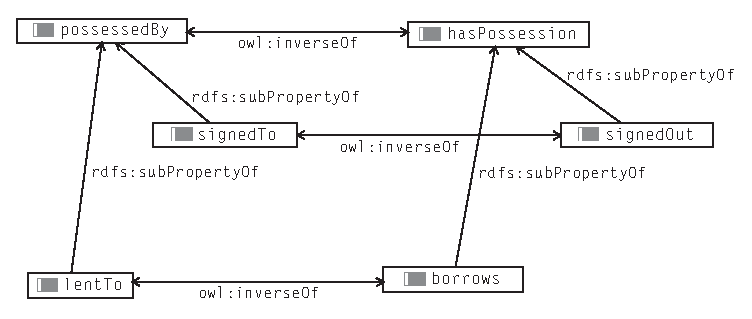
\includegraphics[width=5in]{media/ch9/f09-002.eps}
\caption{Systematic combination of inverseOf and subPropertyOf.}
\label{fig:ch9.2}
\end{figure}


If all we were concerned with was making sure that the inferences about
hasPossession will be supported, then there would be no reason to prefer
one solution over the other. But modeling in the Semantic Web is not
just about supporting desired inferences but also about supporting
reuse. What if someone else
wants to use this model in a slightly different way? A future query is
just as likely to be interested in hasPossession as possessedBy.
Furthermore, we might in the future wish to combine has Possession (or
possessedBy) with another property. For this reason, one might choose to
use both solutions together by using both inverseOf and subPropertyOf in
a systematic way---that is, by specifying inverses for every property,
regardless of the subPropertyOf level. In this case, this results in

\begin{lstlisting}
:signedTo owl:inverseOf :signedOut.
:signedTo rdfs:subPropertyOf :possessedBy.
:signedOut rdfs:subPropertyOf :hasPossession.
:lentTo owl:inverseOf :borrows.
:lentTo rdfs:subPropertyOf :possessedBy.
:borrows rdfs:subPropertyOf :hasPossession.
:possessedBy owl:inverseOf :hasPossession.
\end{lstlisting}

The systematicity of this structure can be more readily seen in Figure
8.2. The attentive reader might have one more concern about the
systematicity of Figure 8.2---in particular, the selection of which
properties are the subject of \texttt{owl:inverseOf} and which are the object (in
the diagram, which ones go on the left or on the right of the diagram)
is arbitrary. Shouldn't there be three more \texttt{owl:inverseOf} triples,
pointing from right to left? Indeed, there should be, but there is no
need to assert these triples, as we shall see in the next challenge.
\end{challenge}


\subsection{Using the modeling language to extend the modeling language}

It is not unusual for beginning modelers to look at the list of
constructs defined in OWL and say, ``There is a feature of the OWL
language I would like to use that is very similar to the ones that are
included. Why did they leave it out? I would prefer to build my model
using a different set of primitives.'' In many cases, the extra language
feature that they desire is actually already supported by OWL as a
combination of other features. It is a simple matter of using these
features in combination.

\begin{challenge}{Superclasses}

For example, RDFS allows you to specify that one class is a subClassOf
another, but you might like to think of it the other way around (perhaps
because of the structure of some legacy data you want to work with) and
specify that something is superClassOf something else. That is, you want
the parent class to be the subject of all the definitional triples.
Using your own namespace myowl: for this desired relation, you would
like to have the triples look like this:

\begin{lstlisting}
:Food myowl:superClassOf :BakedGood; 
      myowl:superClassOf :Confectionary;
      myowl:superClassOf :PackagedFood;
      myowl:superClassOf :PreparedFood;
      myowl:superClassOf :ProcessedFood.
\end{lstlisting}

If we instead use \texttt{rdfs:subClassOf}, all the triples go the other way
around; Food will be the object of each triple, and all the types of
Food will be the subjects.

Since OWL does not provide a superClassOf resource (or to speak more
correctly, OWL does not define any inference rules that will provide any
semantics for a superClassOf resource), what can we do?

\solution

What do we want \texttt{myowl:superClassOf} to mean? For every triple of the form

\begin{lstlisting}
?P myowl:superClassOf ?Q.
\end{lstlisting}

we want to be able to infer that

\begin{lstlisting}
* ?Q rdfs:subClassOf ?P.
\end{lstlisting}

This can be accomplished simply by declaring an inverse

\begin{lstlisting}
myowl:superClassOf owl:inverseOf rdfs:subClassOf.
\end{lstlisting}

It is a simple application of the rule for \texttt{owl:inverseOf} to see that
this accomplishes the desired effect. Nevertheless, this is not a
solution that many beginning modelers think of. It seems to them that
they have no right to modify or extend the meaning of the OWL language
or to make statements about the OWL and RDFS resources (like
\texttt{rdfs:subClassOf}). But remember the AAA slogan of RDF: Anyone can say
Anything about Any topic. In particular, a modeler can say things about
the resources defined in the standard.

In fact, we can take this slogan so far as to allow a modeler to say

\begin{lstlisting}
rdfs:subClassOf owl:inverseOf rdfs:superClassOf.
\end{lstlisting}

This differs from the previous triple in that the subject is a resource
in the (standard) RDFS namespace. The AAA slogan allows a modeler to say
this,  and indeed, there is nothing in the standards that will prevent
it. But this practice is problematic; as we saw in Chapter~\ref{ch5}, it is normally possible to de-reference 
an HTTP URI to learn more about a resource.  Since only the W3C can add new content to the 
web servers at the RDFS namespace, any attempt to de-reference rdfs:superClassOf will fail to return any information. 
Another problem with this practice is that  a reference to a resource in the RDFS namespace 
suggests to human readers of the model that this resource is part of
the RDFS standard (which it is not). Since one purpose of a model is to communicate to
other human beings, it is generally not a good idea to make statements
that are likely to be misleading.   The AAA slogan is like free speech; just because you are 
allowed to say something, doesn't mean that you should. 
\end{challenge}

\subsection{Symmetric  properties in queries}

Consider a simple model about the marriage of Shakespeare---a model with
only one triple.

\begin{lstlisting}
bio:AnneHathaway bio:married lit:Shakespeare.
\end{lstlisting}

If we were to query this with the SPARQL query

\begin{lstlisting}
SELECT ?who
WHERE {?lit:Shakespeare bio:married ?who}
\end{lstlisting}

We would get no answer---Shakespeare married no one, despite our
intuition that marriage is a two-way street. We would like to express
this part of our understanding of how marriage works in a model.

\begin{challenge}{The marriage of Shakespeare}

How can we infer marriages in the reverse direction from which they are
asserted?

\solution

We could do this by simply declaring \texttt{bio:married} to be its own inverse,
thus:

\begin{lstlisting}
bio:married owl:inverseOf bio:married.
\end{lstlisting}

Now any triple that used \texttt{bio:married} would automatically be inferred to
hold in the other direction. In particular, if we asserted

\begin{lstlisting}
bio:AnneHathaway bio:married lit:Shakespeare.
\end{lstlisting}

we could infer that

\begin{lstlisting}
* lit:Shakespeare bio:married bio:AnneHathaway.
\end{lstlisting}

This pattern of self-inverses is so common that it has been built into
OWL using a special construct called
\texttt{owl:SymmetricProperty}.

\subsection{Symmetric Properties}

\texttt{owl:inverseOf} relates one property to another. The special case in which
these two properties are the same (as was the case for \texttt{bio:married} for
the Shakespeare example) is common enough that the OWL language provides
a special name for it: \texttt{owl:SymmetricProperty}. Unlike \texttt{owl:inverseOf},
which is a property that relates two other properties,
\texttt{owl:SymmetricProperty} is just an aspect of a single property and is
expressed in OWL as a Class. We express that a property is symmetric in
the same way as we express membership in any class---in other words:

\begin{lstlisting}
:P a owl:SymmetricProperty.
\end{lstlisting}

As usual, we express the meaning of this statement in SPARQL:

\begin{lstlisting}
CONSTRUCT {?p owl:inverseOf ?p. }
WHERE {?p a owl:SymmetricProperty . }
\end{lstlisting}

So in the case of the marriage of Shakespeare, we can simply assert that

\begin{lstlisting}
bio:married a owl:SymmetricProperty.
\end{lstlisting}
\end{challenge}


\begin{figure}
\centering
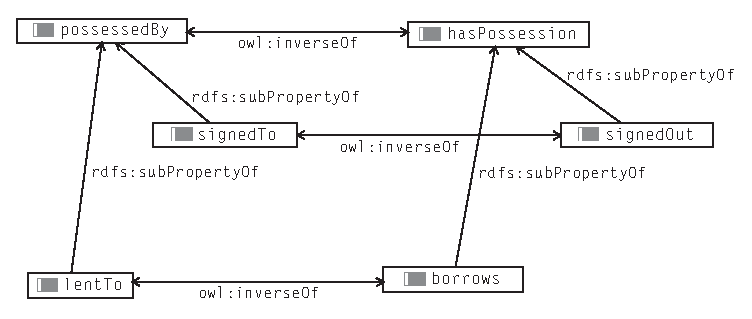
\includegraphics[width=5in]{media/ch9/f09-003.eps}
\caption{Systematic combination of inverseOf and subPropertyOf. Contrast this
with Figure~\ref{fig:ch9.2}, with one- directional inverses.
}
\label{fig:ch9.3}
\end{figure}



\subsection{Using OWL to extend OWL}

As we describe more and more of the power of the OWL modeling language,
there will be more and more opportunities to define at least some
aspects of a new construct in terms of previously defined constructs. We
can use this method to streamline our presentation of the OWL language.
We have seen a need for this already in figure Figure~\ref{fig:ch9.2}, in which all
of our inverses are expressed in one direction but we really need to
have them go both ways, as shown in Figure~\ref{fig:ch9.3}.

We asserted the triples from left to right---namely:

\begin{lstlisting}
:possessedBy owl:inverseOf :hasPossession.
:signedTo owl:inverseOf :signedOut.
:lentTo owl:inverseOf :borrows.
\end{lstlisting}

But we would like to be able to infer the triples from right to
left---namely:

\begin{lstlisting}
:hasPossession owl:inverseOf :possessedBy.
:signedOut owl:inverseOf :signedTo.
:borrows owl:inverseOf :lentTo.
\end{lstlisting}

\begin{challenge}{Modeling self-inverses}

How can we infer all of these triples without having to assert them?

\solution

Since we want \texttt{owl:inverseOf} to work in both directions, this can be done
easily by asserting that
\texttt{owl:inverseOf} is its own inverse, thus:

\begin{lstlisting}
owl:inverseOf owl:inverseOf owl:inverseOf .
\end{lstlisting}



You might have done a double take when you read that \texttt{owl:inverseOf} is
its own inverse. Fortunately, we now have a more readable and somewhat
more understandable way to say this---namely that it is symmetric:

\begin{lstlisting}
owl:inverseOf a owl:SymmetricProperty.
\end{lstlisting}

In either case, we get the inferences we desire for Figure\ref{fig:ch9.3}, in which
the inverses point both ways. This also means that all the inferences in
both directions will always be found.

\subsection{TRANSITIVITY}

In mathematics, a relation R is said to be transitive if $R(a,b)$ and
$R(b,c)$ implies $R(a,c)$. The same idea is used for the OWL construct
\texttt{owl:TransitiveProperty}. Just like \texttt{owl:SymmetricProperty},
\texttt{owl:TransitiveProperty} is a class of properties, so a model can assert
that a property is a member of the class

\begin{lstlisting}
:P a owl:TransitiveProperty.
\end{lstlisting}

The meaning of this is given by a somewhat more elaborate rule than we
have seen so far in this chapter.

\begin{lstlisting}
CONSTRUCT {?x ?p ?z .}
WHERE {?x ?p ?y .
       ?y ?p ?z .
       ?p a owl:TransitiveProperty . }
\end{lstlisting}

Notice that there is no need for even more elaborate rules like

\begin{lstlisting}
CONSTRUCT {?a ?p ?d .}
WHERE {?a ?p ?b .
       ?b ?p ?c .
       ?c ?p ?d . }
\end{lstlisting}

since this conclusion can be reached by applying the simple rule over
and over again.

Some typical examples of transitive properties include
ancestor/descendant (if Victoria is an ancestor of Edward, and Edward is
an ancestor of Elizabeth, then Victoria is an ancestor of Elizabeth) and
geographical containment (if Osaka is in Japan, and Japan is in Asia,
then Osaka is in Asia).

\subsection{Relating parents to ancestors}

A model of genealogy will typically include notions of parents as well
as ancestors, and we'd like them to fit together. But parents are not
transitive (my parents' parents are not my parents), whereas ancestors
are.

\begin{challenge}{Transitive superproperties}
\label{chal:17}
How can we allow a model to maintain consistent ancestry information,
given parentage information?

\solution

Start by defining the parent property to be a subPropertyOf the ancestor
property, thus:

\begin{lstlisting}
:hasParent rdfs:subPropertyOf :hasAncestor.
\end{lstlisting}

Then declare ancestor (only) to be a transitive property:

\begin{lstlisting}
:hasAncestor a owl:TransitiveProperty.
\end{lstlisting}

Let's see how this works on some examples.

\begin{lstlisting}
:Alexia :hasParent :WillemAlexander.
:WillemAlexander :hasParent :Beatrix.
:Beatrix :hasParent :Wilhelmina.
\end{lstlisting}

Because of the \texttt{subPropertyOf} relation between \texttt{hasParent} and \texttt{hasAncestor}
and the fact that
\texttt{hasAncestor} is a \texttt{TransitiveProperty}, we can infer that

\begin{lstlisting}
:Alexia :hasAncestor :WillemAlexander.
:WillemAlexander :hasAncestor :Beatrix.
:Alexia :hasAncestor :Beatrix.
:WillemAlexander :hasAncestor :Wilhelmina.
:Alexia :hasAncestor :Wilhelmina.
\end{lstlisting}

Information about the heritage is integrated, regardless of whether it
originated with \texttt{hasParent} or \texttt{hasAncestor}. Information about hasParent,
on the other hand, is only available as it was directly asserted because
it was not declared to be transitive. The results of this inference are
shown in Figure 8.4.
\end{challenge}

\begin{figure}
\centering
\includegraphics[width=5in]{media/ch9/f09-004.eps}
\caption{Inferences from transitive properties.}
\label{fig:ch9.4}
\end{figure}



\subsection{Layers of relationships}

Sometimes it can be somewhat controversial whether a property is
transitive or not. For instance, the relationship that is often
expressed by the words ``part of'' in English is sometimes transitive (a
piston is part of the engine, and the engine is part of the car; is the
piston part of the car?) and sometimes not (Mick Jagger's thumb is part
of Mick Jagger, and Mick Jagger is part of the Rolling Stones; is Mick
Jagger's thumb part of the Rolling Stones?). In the spirit of
anticipating possible uses of a model, it is worthwhile to support both
points of view whenever there is any chance that controversy might
arise.

\begin{challenge}{Managing transitive relations alongside non-transitive ones}
\label{chal:18}
How can we simultaneously maintain transitive and nontransitive versions
of the \texttt{partOf} information?

\solution

We can define two versions of the \texttt{partOf} property in different
namespaces (or with different names) with one a \texttt{subPropertyOf} the other,
and with the superproperty declared as transitive:

\begin{lstlisting}
dm:partOf rdfs:subPropertyOf gm:partOf.
gm:partOf a owl:TransitiveProperty.
\end{lstlisting}


\begin{figure}
\centering
\includegraphics[width=5in]{media/ch9/f09-005.eps}
\caption{Different interpretations of partOf.}
\label{fig:ch8.5}
\end{figure}



Depending on which interpretation of \texttt{partOf} any particular application
needs, it can query the appropriate property. For those who prefer to
think that Mick Jagger's thumb is not part of the Rolling Stones, the
original \texttt{dm:partOf} property is useful. For those who instead consider
that Mick Jagger's thumb is part of the Rolling Stones, the transitive
superproperty \texttt{gm:partOf} is appropriate (see Figure\label{fig:ch8.5})
\end{challenge}

\section{Managing networks of dependencies}

The same modeling patterns we have been using to manage relationships
(like ancestry) or set containment (like part of) can be used just as
well in a very different setting---namely, to manage networks of
dependencies. In the series of challenges that follow, we will see how
the familiar constructs of \texttt{rdfs:subPropertyOf}, \texttt{owl:inverseOf}, and
\texttt{owl:TransitiveProperty} can be combined in novel ways to model important
aspects of such networks.

A common application of this idea is in workflow management. In a
complex working situation, a variety of tasks must be repeatedly
performed in a set sequence. The idea of workflow management is that the
sequence can be represented explicitly and the progress of each task
tracked in that sequence. Why would someone want to model workflow in a
Semantic Web? The answer is for the same reason one wants to put
anything on the Web: so that parts of the workflow can be shared with
others, encouraging reuse, review, and publication of work fragments.

Real workflow specifications are far too detailed to serve as examples
in a book, so we will use a simple example to show how it works. Let's
make some ice cream, using the following recipe:


\begin{quote}
Slice a vanilla bean lengthwise, and scrape the contents into 1 cup of
heavy cream. Bring the mixture to a simmer, but do not boil. While the
cream is heating, separate three eggs. Add 1/2 cup white sugar to the
eggs and beat until fluffy. Gradually add the warm cream, beating
constantly. Return the custard mixture to medium heat, and cook until
mixture leaves a heavy coat on the back of a spatula. Chill well. Combine custard with 1 cup whole milk, and turn in ice cream freezer according to manufacturer's instructions.
\end{quote}



\begin{figure}
\centering
\includegraphics[width=5in]{media/ch9/f09-006.eps}
\caption{Dependencies for homemade ice cream.}
\label{fig:ch9.6}
\end{figure}


First, let's use a property \texttt{dependsOn} to represent the dependencies
between the steps and define its inverse enables, since each step
enables the next in the correct execution of the workflow:

\begin{lstlisting}
:dependsOn owl:inverseOf :enables.
\end{lstlisting}

Now we can define the dependency structure of the recipe steps:

\begin{lstlisting}
:SliceBean :enables :HeatCream.
:SeparateEggs :enables :AddSugar.
:AddSugar :enables :BeatEggs
:BeatEggs :enables :GraduallyMix.
:HeatCream :enables :GraduallyMix.
:GraduallyMix :enables :CookCustard.
:CookCustard :enables :Chill.
:Chill :enables :AddMilk.
:AddMilk :enables :TurnInFreezer.
\end{lstlisting}

Because of the \texttt{inverseOf}, we can view these steps either in enabling
order as asserted or in dependency order, as shown in Figure\ref{fig:ch9.6}.

\begin{challenge}{Managing an ice-cream recipe}

For any particular step in the process, we might want to know all the
steps it depends on or all the steps that depend on it. How can we do
this, using the patterns we already know?

\solution

We can use the \texttt{subPropertyOf}/\texttt{TransitiveProperty} pattern for each of
dependsOn and
enables as follows:

\begin{figure}
\centering
\includegraphics[width=5in]{media/ch9/f09-007.eps}
\caption{Transitive properties hasPrerequisite and prerequisiteFor defined in
terms of dependsOn and enables.
}
\label{fig:ch9.7}
\end{figure}



These relationships can be seen graphically in Figure\ref{fig:ch9.7}

From these triples, for instance, we can infer that GraduallyMix has
five prerequisites---
namely:

\begin{lstlisting}
* :GraduallyMix :hasPrerequisite :AddSugar ;
*               :hasPrerequisite :SeparateEggs ;
*               :hasPrerequisite :SliceBean ;
*               :hasPrerequisite :HeatCream ;
*               :hasPrerequisite :BeatEggs .
\end{lstlisting}
\end{challenge}


\begin{challenge}{Managing workflow}

In a more realistic workflow management setting, we wouldn't just be
managing a single process (corresponding to a single recipe). We would
be managing several processes that interact in complex ways. We could
even lose track of which steps are in the same procedure. Is there a way
to find out, given a particular step, what the other steps in the same
process are? In our recipe example, can we model the relationship
between steps so that we can connect steps in the same recipe together?

\solution

First, we combine together both of our fundamental relationships
(\texttt{enables} and \texttt{dependsOn}) as common \texttt{subPropertyOf} a single unifying
property (\texttt{neighborStep}). We then, in turn, make that a \texttt{subPropertyOf} of
a transitive property (\texttt{inSameRecipe}), shown here in Turtle and in Figure~\ref{fig:ch9.8}(a).

\begin{lstlisting}
:dependsOn rdfs:subPropertyOf :neighborStep.
:enables rdfs:subPropertyOf :neighborStep.
:neighborStep rdfs:subPropertyOf :inSameRecipe.
:inSameRecipe a owl:TransitiveProperty.
\end{lstlisting}

What inferences can we draw from these triples for the instance
\texttt{GraduallyMix}? Any directly related step (related by either \texttt{dependsOn} or
\texttt{enables}) becomes a \texttt{neighborStep}, and any combination of neighbors is
rolled up with \texttt{inSameRecipe}. A few selected inferences are shown here:

\begin{lstlisting}
:GraduallyMix :neighborStep :BeatEggs ;
              :neighborStep :HeatCream ;
              :neighborStep :CookCustard .
:CookCustard  :neighborStep :Chill ;
              :neighborStep :GraduallyMix .
:GraduallyMix :inSameRecipe :BeatEggs ;
              :inSameRecipe :HeatCream ;
              :inSameRecipe :CookCustard .
:CookCustard  :inSameRecipe :Chill ;
              :inSameRecipe :GraduallyMix .
        ...
:GraduallyMix :inSameRecipe :AddMilk ;
              :inSameRecipe :CookCustard ;
              :inSameRecipe :TurnInFreezer ;
              :inSameRecipe :AddSugar ;
              :inSameRecipe :SeparateEggs ;
              :inSameRecipe :SliceBean ;
              :inSameRecipe :HeatCream ;
              :inSameRecipe :GraduallyMix ;
              :inSameRecipe :Chill ;
              :inSameRecipe :BeatEggs .
\end{lstlisting}



\begin{figure}
\centering
\includegraphics[width=5in]{media/ch9/f09-008.eps}
\caption{Contrast patterns for inSameRecipe (includes self) and otherStep
(excludes self). Both patterns work from the same input properties
dependsOn and enables but yield different results.}
\label{fig:ch9.8}
\end{figure}



All the steps in this recipe have been gathered up with \texttt{inSameRecipe}, as
desired. In fact, any two steps in this recipe will be related to one
another by \texttt{inSameRecipe}, including relating each step to itself. In
particular, the triple

\begin{lstlisting}
:GraduallyMix :inSameRecipe :GraduallyMix.
\end{lstlisting}

has been inferred. Although this is, strictly speaking, correct (after
all, indeed \texttt{GraduallyMix} is in the same recipe as \texttt{GraduallyMix}), it
might not be what we actually wanted to know.
\end{challenge}


\begin{challenge}{Finding other steps}

How can we define a property that will relate a recipe step only to the
other steps in the same recipe?

\solution

Earlier we defined two properties, \texttt{hasPrerequisite} and \texttt{prerequisiteFor},
one looking ``downstream'' along the dependencies and one looking
``upstream.''

\begin{lstlisting}
:dependsOn rdfs:subPropertyOf :hasPrerequisite.
:hasPrerequisite a owl:TransitiveProperty.
:enables rdfs:subPropertyOf :prerequisiteFor.
:prerequisiteFor a owl:TransitiveProperty.
\end{lstlisting}

If we join these two together under a common superproperty that is not
transitive, we get the following:

\begin{lstlisting}
:hasPrerequisite rdfs:subPropertyOf :otherStep .
:prerequisiteFor rdfs:subPropertyOf :otherStep .
\end{lstlisting}

These relationships are shown diagrammatically in Figure\ref{fig:ch9.8}(b).

We track the inferences separately for each property. For
\texttt{hasPrerequisite}, we have already seen that we can infer the following:

\begin{lstlisting}
:GraduallyMix :hasPrerequisite :AddSugar ;
              :hasPrerequisite :SeparateEggs ;
              :hasPrerequisite :SliceBean ;
              :hasPrerequisite :HeatCream ;
              :hasPrerequisite :BeatEggs .
\end{lstlisting}

For \texttt{prerequisiteFor}, we get the following inferences:

\begin{lstlisting}
:GraduallyMix :prerequisiteFor :AddMilk ;
              :prerequisiteFor :CookCustard ;
              :prerequisiteFor :TurnInFreezer ;
              :prerequisiteFor :Chill .
\end{lstlisting}

Now, for otherStep, we get the combination of these two. Notice that
neither list includes Gradually
Mix itself, so it does not appear in this list either.

\begin{lstlisting}
:GraduallyMix :otherStep :AddMilk ;
              :otherStep :CookCustard ;
              :otherStep :TurnInFreezer ;
              :otherStep :AddSugar ;
              :otherStep :SeparateEggs ;
              :otherStep :SliceBean ;
              :otherStep :HeatCream ;
              :otherStep :Chill ;
              :otherStep :BeatEggs .
\end{lstlisting}

Figure\ref{fig:ch9.8} shows the two patterns. For \texttt{inSameRecipe}, we have a single
transitive property at the top of a subPropertyOf tree; both primitive
properties (\texttt{enables} and \texttt{dependsOn}) are brought together, and any
combinations of the resulting property (\texttt{neighborStep}) are chained
together as a TransitiveProperty (\texttt{inSameRecipe}). For otherStep, the
top-level property itself is not transitive but is a simple combination
(via two subPropertyOf links) of two transitive properties
(\texttt{hasPrerequisite} and \texttt{prerequisiteFor}). Inference for each of these
transitive properties is done separately from the other, and the results
combined (without any more transitive interaction). Hence, for
\texttt{inSameRecipe}, the reflexive triples like

\begin{lstlisting}
:GraduallyMix :inSameRecipe :GraduallyMix
\end{lstlisting}

are included, whereas for \texttt{otherStep}, they are not.

Another ramification of the difference between these two models has to
do with whether or not they can ``turn the corner'' in Figure~\ref{fig:ch9.6} and
determine a relationship between, e.g., \texttt{BeatEggs} and \texttt{HeatCream}. The
transitive structure of \texttt{inSameRecipe} allows this to happen, whereas for
\texttt{otherStep} it does not; that is, we can infer

\begin{lstlisting}
\begin{lstlisting}
:BeatEggs :inSameRecipe :HeatCream
end{lstlisting}
but not
:BeatEggs :otherStep :HeatCream .
\end{lstlisting}
\end{challenge}

\section{Equivalence}
\label{section:Equivalence}
RDF provides a global notion of identity that has validity across data
sources; that global identity is the URI. This makes it possible to
refer to a single entity in a distributed way. But when we want to merge
information from multiple sources controlled by multiple stakeholders,
it is not necessarily the case that any two stakeholders will use the
same URI to refer to the same entity. Thus, in a federated information
setting, it is useful to be able to stipulate that two URIs actually
refer to the same entity. But there are different ways in which two
entities can be the same. Some are more equal than others. RDFS-Plus
provides a variety of notions of equivalence. As with other constructs
in OWL, these different constructs are defined by the inferences they
entail.

\subsection{Equivalent classes}

We previously used a simple idiom to express that one class had the same
elements as another; in particular, we asserted two triples

\begin{lstlisting}
:Analyst rdf:subClassOf :Researcher.
:Researcher rdf:subClassOf :Analyst.
\end{lstlisting}

to indicate that every Analyst is a Researcher and every Researcher is
an Analyst. As we saw, the rule for \texttt{rdf:subClassOf} can be applied in
each direction to support the necessary inferences to make every Analyst
a Researcher and vice versa. When two classes are known to always have
the same members, we say that the classes are equivalent. The preceding
pattern allows us to express class equivalence in RDFS, if in a somewhat
unintuitive way.

RDFS-Plus provides a more intuitive expression of class equivalence,
using the construct

\texttt{owl:equivalentClass}. A single triple expresses class equivalence in the
obvious way:

\begin{lstlisting}
:Analyst owl:equivalentClass :Researcher.
\end{lstlisting}

As with any other construct in RDFS or OWL, the precise meaning of
\texttt{owl:equivalentClass} is given by the inferences that can be drawn, which
we express in SPARQL:

\begin{lstlisting}
CONSTRUCT {?r a ?b .}
WHERE {?a owl:equivalentClass ?b .
       ?r a ?a . }
\end{lstlisting}

So far, this is just the type propagation rule that we used to define
the meaning of \texttt{rdf:subClassOf} in Chapter\ref{ch7}. But \texttt{owl:equivalentClass} has another rule as
well:

\begin{lstlisting}
CONSTRUCT {?r a ?a .}
WHERE {?a owl:equivalentClass ?b .
       ?r a ?b . }
\end{lstlisting}

That is, the two classes \texttt{?a} and \texttt{?b} have exactly the same members.

It seems a bit of a shame that something as simple as equivalence
requires two rules to express, especially when the rules are so similar.
In fact, this isn't necessary; if we observe that

\begin{lstlisting}
owl:equivalentClass a owl:SymmetricProperty.
\end{lstlisting}

then there is no need for the second rule; we can infer it from the
first rule and the symmetry of
equivalentClass.

In fact, we don't actually need any rules at all; if we also assert that

\begin{lstlisting}
owl:equivalentClass rdfs:subPropertyOf rdfs:subClassOf.
\end{lstlisting}

we can use the rules for subPropertyOf and subClassOf to infer
everything about equivalentClass! Let's see how the rules for OWL, which
we have already learned work for \texttt{owl:equivalentClass}, in the case of the
Analyst and the Researcher.

From the rule about \texttt{rdfs:subClassOf} and the statement of equivalence of
Analyst and
Researcher, we can infer that

\begin{lstlisting}
:Analyst rdfs:subClassOf :Researcher.
\end{lstlisting}

But since \texttt{owl:equivalentClass} is symmetric, we can also infer that

\begin{lstlisting}
* :Researcher owl:equivalentClass :Analyst.
\end{lstlisting}

and by applying the rule for \texttt{rdfs:subClassOf} once again, we get

\begin{lstlisting}
* :Researcher rdfs:subClassOf :Analyst.
\end{lstlisting}

That is, simply by applying what we already know about \texttt{rdfs:subClassOf}
and \texttt{owl:SymmetricProperty}, we can infer both \texttt{rdfs:subClassOf} triples
from the single \texttt{owl:equivalentClass} triple.

Notice that when two classes are equivalent, it only means that the two
classes have the same members. Other properties of the classes are not
shared; for example, each class keeps its own
\texttt{rdfs:label}. This means that if these classes have been merged from two
different applications, each of these applications will still display
the class by the original print name; only the members of the class will
change.

\subsection{Equivalent properties}

We have seen how to use \texttt{rdfs:subPropertyOf} to make two properties behave
in the same way; the trick we used there was very similar to the double
subClassOf trick. We use \texttt{rdfs:subPropertyOf} twice to indicate that two
properties are equivalent.

\begin{lstlisting}
:borrows rdfs:subPropertyOf :checkedOut.
:checkedOut rdfs:subPropertyOf :borrows.
\end{lstlisting}

RDFS-Plus also provides a more intuitive way to express property
equivalence, using
owl:equivalentProperty, as follows:

\begin{lstlisting}
:borrows owl:equivalentProperty :checkedOut.
\end{lstlisting}

When two properties are equivalent, we expect that in any triple that
uses one as a predicate, the other can be substituted---this is, we can
define it in SPARQL with

\begin{lstlisting}
CONSTRUCT {?a :checkedOut ?b . }
WHERE {?a :borrows ?b . }
\end{lstlisting}

and vice versa. We can accomplish this in a manner analogous to the
method used for \texttt{owl:equivalentClass}. We define \texttt{owl:equivalentProperty} in
terms of other RDFS-Plus constructs.

\begin{lstlisting}
owl:equivalentProperty rdfs:subPropertyOf rdfs:subPropertyOf.
owl:equivalentProperty a owl:SymmetricProperty.
\end{lstlisting}

Starting with the asserted equivalence of \texttt{borrows} and \texttt{checkedOut}, using
these triples, and the rules for \texttt{rdfs:subPropertyOf} and
\texttt{owl:SymmetricProperty}, we can infer that

\begin{lstlisting}
:borrows rdfs:subPropertyOf checkedOut.
:checkedOut owl:equivalentProperty borrows.
:checkedOut rdfs:subPropertyOf borrows.
\end{lstlisting}

Once we have inferred that \texttt{borrows} and \texttt{checkedOut} are \texttt{rdfs:subPropertyOf}
one another, we can make all the appropriate inferences.

When we express new constructs (like \texttt{owl:equivalentProperty} in this
section) to constructs we already know (\texttt{rdfs:subPropertyOf} and
\texttt{owl:SymmetricProperty}), we explicitly describe how the various parts of
the language fit together. That is, rather than just noticing that the
rule governing \texttt{owl:equivalent} Property is the same rule as the one that
governs \texttt{rdfs:subPropertyOf} (except that it works both ways!), we can
actually model these facts. By making \texttt{owl:equivalentProperty} a
subproperty of \texttt{rdfs:subPropertyOf}, we explicitly assert that they are
governed by the same rule. By making \texttt{owl:equivalentProperty} an
\texttt{owl:SymmetricProperty}, we assert the fact that this rule
works in both directions. This makes the relationship between the parts
of the OWL language explicit and, in fact, models them in OWL.

\subsection{Same individuals}

Class equivalence---that is, \texttt{owl:equivalentClass}---and property
equivalence (\texttt{own:equivalentProperty}) provide intuitive ways to express
relationships that were already expressible in RDFS. In this sense,
neither of these constructs has increased the expressive power of
RDFS-Plus beyond what was already available in RDFS. They have just made
it easier to express and clearer to read. These constructs refer
respectively to classes of things and the properties that relate them.

But when we are describing things in the world, we aren't only
describing classes and properties; we are describing the things
themselves. These are the members of the classes. We refer to these as
\emph{individuals}. We have encountered a number of individuals in our examples
so far---Wenger the Analyst, Kildare the Surgeon, Kaneda the All-Star
Player---and any number of things whose class membership has not been
specified---Wales, The Firm, and Moby Dick. But remember the nonunique
naming assumption: Often, our information comes from multiple sources
that might not have done any coordination in their reference to
individuals. How do we handle the situation in which we determine that
two individuals that we originally thought of separately are in fact the
same individual?

In RDFS-Plus, this is done with the single construct \texttt{owl:sameAs}. Our old
friend William Shakespeare will provide us with an example of how
\texttt{owl:sameAs} works. From Chapter\ref{ch3}, we have the following triples about
the literary career of William Shakespeare:

\begin{lstlisting}
lit:Shakespeare lit:wrote lit:AsYouLikeIt ;
                lit:wrote lit:HenryV ;
                lit:wrote lit:LovesLaboursLost ;
                lit:wrote lit:MeasureForMeasure ; 
                lit:wrote lit:TwelfthNight ;
		lit:wrote lit:WintersTale ; 
                lit:wrote lit:Hamlet ;
                lit:wrote lit:Othello .
\end{lstlisting}

Suppose we have at our disposal information from the Stratford Parish
Register, which lists the following information from some baptisms that
occurred there. We will use \texttt{spr:} as the namespace identifier for URIs
from the Stratford Parish Register.

\begin{lstlisting}
spr:Gulielmus spr:hasFather spr:JohannesShakspere .
spr:Susanna spr:hasFather spr:WilliamShakspere .
spr:Hamnet spr:hasFather spr:WilliamShakspere .
spr:Judeth spr:hasFather spr:WilliamShakspere .
\end{lstlisting}

Suppose that our research determines that, indeed, the resources
mentioned here as \texttt{spr:Gulielmus}, \texttt{spr:WilliamShakspere}, and
\texttt{lit:Shakespeare} all refer to the same individual, so the answer to the
question ``Did Hamnet's father write Hamlet ?'' would be ``yes.'' If we
had known that all of these things refer to the same person in advance
of having represented the Stratford Parish Register in RDF, we could
have used the same URI (e.g., \texttt{lit:Shakespeare}) for
each occurrence of the Bard. But we are living in the data wilderness,
and now it is too late; the URIs from each data source have already been
chosen. What is to be done?

First, let's think about how to pose the question ``Did Hamnet's father
write Hamlet ?'' We can write this as a graph pattern in SPARQL as
follows:

\begin{lstlisting}
{spr:Hamnet spr:hasFather ?d .
 ?d lit:wrote lit:Hamlet . }
\end{lstlisting}

that is, we are looking for a single resource that links Hamnet to
Hamlet via the two links
\texttt{spr:hasFather} and \texttt{lit:wrote}.


In RDFS-Plus, we have the option of asserting the sameness of two
resources. Let's start with just one:

\begin{lstlisting}
spr:WilliamShakspere owl:sameAs lit:Shakespeare .
\end{lstlisting}

The meaning of this triple, as always in RDFS-Plus, is expressed by the
inferences that can be drawn. The rule for \texttt{owl:sameAs} is quite
intuitive; it says that if A \texttt{owl:sameAs} B, then in any triple where we
see A, we can infer the same triple, with A replaced by B. So for our
Shakespeare example, the inference is defined as

\begin{lstlisting}
CONSTRUCT {lit:Shakespeare ?p ?o . }
WHERE {spr:WilliamShakespeare ?p ?o . }
\end{lstlisting}

Similarly,

\begin{lstlisting}
CONSTRUCT {?s ?p lit:Shakespeare . }
WHERE {?s ?p spr:WilliamShakespeare . }
\end{lstlisting}

More generally, \texttt{owl:sameAs} is defined by three rules that can be
expressed in SPARQL as

\begin{lstlisting}
CONSTRUCT {?s ?p ?x . }
WHERE {?s ?p ?y .
       ?x owl:sameAs ?y .}
\end{lstlisting}

\begin{lstlisting}
CONSTRUCT {?x ?p ?o . }
WHERE {?y ?p ?o .
       ?x owl:sameAs ?y .} 
\end{lstlisting}

\begin{lstlisting}
CONSTRUCT {?s ?x ?o . }
WHERE {?s ?y ?o .
       ?x owl:sameAs ?y .}
\end{lstlisting}

Also, as we did for \texttt{owl:equivalentClass} and \texttt{owl:equivalentProperty}, we
assert that \texttt{owl:sameAs} is an \texttt{owl:SymmetricProperty}:

\begin{lstlisting}
owl:sameAs a owl:SymmetricProperty .
\end{lstlisting}

Otherwise, we would need three more rules, with the \texttt{owl:sameAs} triples
reversed. This allows us to infer that

\begin{lstlisting}
lit:Shakespeare owl:sameAs spr:WilliamShakspere .
\end{lstlisting}

so that we can replace any occurrence of \texttt{lit:Shakespeare} with
\texttt{spr:WilliamShakspere}
as well.

Let's see how this works with the triples we know from literary history
and the Register. We list all triples, with asserted triples in Roman
and inferred triples in italics. Among the inferred triples, we
begin by replacing \texttt{lit:Shakespeare} with \texttt{spr:WilliamShakspere}, then
continue by replacing \texttt{spr:WilliamShakspere} with \texttt{lit:Shakespeare}:

\begin{lstlisting}
lit:Shakespeare lit:wrote lit:AsYouLikeIt ;
                lit:wrote lit:HenryV ;
		lit:wrote lit:LovesLaboursLost ;
		lit:wrote lit:MeasureForMeasure ;
		lit:wrote lit:TwelfthNight ;
		lit:wrote lit:WintersTale ;
		lit:wrote lit:Hamlet ;
		lit:wrote lit:Othello .
spr:Gulielmus spr:hasFather spr:JohannesShakspere .
spr:Susanna spr:hasFather spr:WilliamShakspere .
spr:Hamnet spr:hasFather spr:WilliamShakspere .
spr:Judeth spr:hasFather spr:WilliamShakspere .
spr:WilliamShakspere lit:wrote lit:AsYouLikeIt ;  
                     lit:wrote lit:HenryV ;
		     lit:wrote lit:LovesLaboursLost ;
		     lit:wrote lit:MeasureForMeasure ;
		     lit:wrote lit:TwelfthNight ;
		     lit:wrote lit:WintersTale ;
		     lit:wrote lit:Hamlet ;
		     lit:wrote lit:Othello .
spr:Susanna spr:hasFather lit:Shakespeare .
spr:Hamnet spr:hasFather lit:Shakespeare .
spr:Judeth spr:hasFather lit:Shakespeare .
\end{lstlisting}

Now the answer to the query ``Did Hamnet's father write Hamlet ?'' is
``yes,'' since there is a binding for the variable \texttt{?d} in the preceding
SPARQL graph pattern. In fact, there are two possible bindings:

\texttt{?d} = \texttt{lit:Shakespeare} and \texttt{?d} = \texttt{spr:Shakspere}.
\end{challenge}


\section{Merging data from different databases}

We have seen how to interpret information in a table as RDF triples.
Each row in the table became a single individual, and each cell in the
table became a triple. The subject of the triple is the individual
corresponding to the row that the cell is in; the predicate is made up
from the table name and the field name; and the object is the cell
contents. Table 8.1 (from Table 3.10) shows
63 triples for the 7 fields and 9 rows. Let's look at just the triples
having to do with the
Manufacture\_Location.

\begin{lstlisting}
mfg:Product1 mfg:Product_Manufacture_Location Sacramento.
mfg:Product2 mfg:Product_Manufacture_Location Sacramento.
mfg:Product3 mfg:Product_Manufacture_Location Sacramento.
mfg:Product4 mfg:Product_Manufacture_Location Elizabeth.
mfg:Product5 mfg:Product_Manufacture_Location Elizabeth.
mfg:Product6 mfg:Product_Manufacture_Location Seoul.
mfg:Product7 mfg:Product_Manufacture_Location Hong Kong.
mfg:Product8 mfg:Product_Manufacture_Location Cleveland.
mfg:Product9 mfg:Product_Manufacture_Location Cleveland.
\end{lstlisting}


\begin{table}
\label{tab:ch9.1}
\caption{Sample tabular data for triples}
\begin{tabular}{|l l l l l l l|}
\hline
ID&Model Number&Division&Product Line&Manufacture Location&SKU&Available\\
\hline
1&ZX-3&Manufacturing Support&Paper Machine&Sacramento&FB3524&23\\
2&ZX-3P&Manufacturing Support&Paper Machine&Sacramento&KD5243&4\\
3&ZX-3S&Manufacturing Support&Paper Machine&Sacramento&IL4028&34\\
4&B-1430&Control Engineering&Feedback Line&Elizabeth&KS4520&23\\
5&B-1430X&Control Engineering&Feedback Line&Elizabeth&CL5934&14\\
6&B-1431&Control Engineering&Active Sensor&Seoul&KK3945&0\\
7&DBB-12&Accessories&Monitor&Hong Kong&ND5520&100\\
8&SP-1234&Safety&Safety Valve&Cleveland&HI4554&4\\
9&SPX-1234&Safety&Safety Valve&Cleveland&OP5333&14\\
\hline
\end{tabular}
\end{table}

\begin{table}
\label{tab:ch9.2}
\caption{Sample Data: Parts and the Facilities Required to Produce Them}
\begin{tabular}{|l l l|}
\hline
ID&Model Number&Facility\\
\hline
1&B-1430&Assembly Center\\
2&B-1431&Assembly Center\\
3&M13-P&Assembly Center\\
4&ZX-3S&Assembly enter\\
5&ZX-3&Factory\\
6&TC-43&Factory\\
7&B-1430X&Machine Shop\\
8&SP-1234&Machine Shop\\
9&1180-M&Machine Shop\\
\hline
\end{tabular}
\end{table}

Suppose that another division in the company keeps its own table of the
products with information that is useful for that division's business
activities---namely, it describes the sort of facility that is required
to produce the part. Table~\ref{tab:ch9.2} shows some products and the facilities
they require. Some of the products in Table~\ref{tab:ch9.2} also appeared in Table~\ref{tab:ch9.1}, and some did not. It is not uncommon for different databases to
overlap in such an inexact way.

\begin{challenge}{Merging tables}

Using the products that appear in both tables, how can we write a
federated query that will cross-reference cities with the facilities
that are required for the production that takes place there?

\solution

If these two tables had been in a single database, then there could have
been a foreign-key reference from one table to the other, and we could
have joined the two tables together. Since the tables come from two
different databases,
there is no such common reference. This is typical of data found in the
wilderness; no effort has been made to align data from different
sources.

When we turn both tables into triples, the individuals corresponding to
each row are assigned global identifiers.

Suppose that we use the namespace \texttt{p:} for the second database; when we
turn  Table~\ref{tab:ch9.2} into triples, we get 27 triples, for the 9 rows and 3
fields. The triples corresponding to the required facilities are as
follows:

\begin{lstlisting}
p:Product1 p:Product_Facility "Assembly Center" .
p:Product2 p:Product_Facility "Assembly Center" .
p:Product3 p:Product_Facility "Assembly Center" .
p:Product4 p:Product_Facility "Assembly Center" .
p:Product5 p:Product_Facility "Factory" .
p:Product6 p:Product_Facility "Factory" .
p:Product7 p:Product_Facility "Machine Shop" .
p:Product8 p:Product_Facility "Machine Shop" .
p:Product9 p:Product_Facility "Machine Shop" .
\end{lstlisting}

Although we have global identifiers for individuals in these tables,
those identifiers are not the same. For instance, p:Product1 is the same
as mfg:Product4 (both correspond to model number B-1430). How can we
cross-reference from one table to the other? The answer is to use a
series of \texttt{owl:sameAs} triples, as follows:

\begin{lstlisting}
p:Product1 owl:sameAs mfg:Product4 .
p:Product2 owl:sameAs mfg:Product6 .
p:Product4 owl:sameAs mfg:Product3 .
p:Product5 owl:sameAs mfg:Product1 .
p:Product7 owl:sameAs mfg:Product5 .
p:Product8 owl:sameAs mfg:Product8 .
\end{lstlisting}

Now if we match the following SPARQL graph pattern:

\begin{lstlisting}
{?p p:Product_Facility ?facility.
 ?p mfg:Product_Manufacture_Location ?location.}
\end{lstlisting}

and display \texttt{?facility} and \texttt{?location}, we get the results in Table\ref{tab:ch9.3}.
\end{challenge}

This solution has addressed the challenge for the particular data in the
example, but the solution relied on the fact that we knew which product
from one table matched with which product from another table. But
\texttt{owl:sameAs} only solves part of the problem. In real data situations, in
which the data in the tables change

\begin{table}
\label{tab:ch9.3}
\caption{Locations Cross-Referenced with Facilities, Computed via
Products}
\begin{tabular}{|ll|}
\hline
?location&?facility\\
\hline
Elizabeth&Assembly Center\\
Seoul&Assembly Center\\
Sacramento&Assembly Center\\
Sacramento&Factory\\
Elizabeth&Machine Shop\\
Cleveland&Machine Shop \\
\hline
\end{tabular}
\end{table}

frequently, it is not practical to assert all the \texttt{owl:sameAs} triples by
hand. In the next section, we will see how
RDFS-Plus provides a solution to the rest of the challenge.

\section{Computing Sameness: Functional Properties}

Functional Properties in OWL get their name from a concept in
mathematics, but like most of the OWL constructs, they have a natural
interpretation in everyday life. A functional property is one for which
there can be just one value. Examples of such properties are quite
common: \texttt{hasMother} (since a person has just one biological mother),
\texttt{hasBirthplace} (someone was born in just one place), and \texttt{birthdate} (just
one) are a few simple examples.

In mathematics, a function is a mapping that gives one value for any
particular input, so $x^2$ is
a function, since for any value of $x$, there is exactly one value for $x^2$.
Another way to say this is that if
$x = y$, then $x^2 = y^2$. To solve the previous challenge problem, we have to
have constructs in RDFS-Plus that have this same sort of behavior; that
is, we want to describe something as being able to refer to only a
single value.

The next two constructs, \texttt{FunctionalProperty} and
\texttt{InverseFunctionalProperty}, use this idea to determine when two resources
refer to the same individual, thereby providing the OWL modeler with a
means for describing how information from multiple sources are to be
considered as a distributed web of information. These constructs provide
an important semantic framework for using RDFS-Plus in the Semantic Web
setting.

\subsection{Functional properties}

RDFS-Plus borrows the name \emph{functional} to describe a property that, like
a mathematical function, can only take one value for any particular
individual. The precise details of the meaning of \texttt{owl:FunctionalProperty}
is given, as usual, as an inference pattern expressed in SPARQL:

\begin{lstlisting}
CONSTRUCT {?a owl:sameAs ?b . }
WHERE {?p a owl:FunctionalProperty .
       ?x ?p ?a .
       ?x ?p ?b . }
\end{lstlisting}

This definition of \texttt{owl:FunctionalProperty} is analogous to the
mathematical situation in which we know that $x^2$ has a single unambiguous
value. More precisely, if we know that $x^2 = a$ and $x^2 = b$, then we may
conclude that $a = b$. In RDFS-Plus, this looks as follows, in which the
first three triples are asserted and the fourth is inferred:

\begin{lstlisting}
math:hasSquare a owl:FunctionalProperty.
:x math:hasSquare :A.
:x math:hasSquare :B.
:A owl:sameAs :B.
\end{lstlisting}

Functional properties are important in RDFS-Plus because they allow
sameness to be inferred. For instance, suppose that in the Stratford
Parish Registry we have an entry that tells us

\begin{lstlisting}
lit:Shakespeare fam:hasFather bio:JohannesShakspere .
\end{lstlisting}

and that from Shakespeare's grave we learn that

\begin{lstlisting}
lit:Shakespeare fam:hasFather bio:JohnShakespeare .
\end{lstlisting}

We would like to conclude that John and Johannes are in fact the same
person. If we know from a background model of family relationships that

\begin{lstlisting}
fam:hasFather a owl:FunctionalProperty .
\end{lstlisting}

then we can conclude, from the definition of \texttt{owl:FunctionalProperty},
that

\begin{lstlisting}
* bio:JohannesShakspere owl:sameAs bio:JohnShakespeare .
\end{lstlisting}

as desired.

Although \texttt{owl:FunctionalProperty} provides us with a means of concluding
that two resources are the same, this is not the usual pattern for
determining that two entities are the same in most real data. Much more
common is the closely related notion of \texttt{owl:InverseFunctionalProperty},
which we treat next.

\subsection{Inverse functional properties}

Some people consider \texttt{owl:InverseFunctionalProperty} to be the most
important modeling construct in RDFS-Plus, especially in situations in
which a model is being used to manage data from multiple sources.
Whether or not this is true, it is certainly true that it has the most
difficult name with respect to its utility of any construct.

The name \texttt{owl:InverseFunctionalProperty} was chosen to be consistent with
the closely related \texttt{owl:FunctionalProperty}, and in fact one can think of
an \texttt{owl:InverseFunctionalProperty} simply as the inverse of an
\texttt{owl:FunctionalProperty}. So if \texttt{math:hasSquare} is a functional property,
then its inverse, \texttt{math:hasSquareRoot}, is an inverse functional
property.

What exactly does this mean in terms of inferences that can be drawn?
The rule looks very similar to the rule for \texttt{owl:FunctionalProperty},

\begin{lstlisting}
CONSTRUCT {?a owl:sameAs ?b . }
WHERE {?p a owl:InverseFunctionalProperty .
       ?a ?p ?x .
       ?b ?p ?x . }
\end{lstlisting}

For example, if we define a property buriedAt to be sufficiently
specific that we cannot have two people buried at the same location,
then we can declare it to be an \texttt{owl:InverseFunctionalProperty}. If we
were then to have two triples that assert

\begin{lstlisting}
spr:Shakespere buriedAt:TrinityChancel .
lit:Shakespeare buriedAt:TrinityChancel .
\end{lstlisting}

then we could infer that

\begin{lstlisting}
* spr:Shakespere owl:sameAs lit:Shakespeare .
\end{lstlisting}

an \texttt{owl:InverseFunctionalProperty} plays a similar role as a key field in
a relational database. A single value of the property cannot be shared
by two entities, just as a key field may not be
duplicated in more than one row. Unlike the case of a relational
database, RDFS-Plus does not signal an error if two entities are found
to share a value for an inverse functional property. Instead, RDFS-Plus
infers that the two entities must be the same. Because of the nonunique
naming assumption, we cannot tell that two entities are distinct just by
looking at their URIs.

Examples of inverse functional properties are fairly commonplace; any
identifying number (Social Security number, employee number, driver's
license number, serial number, etc.) is an inverse functional property.
In some cases, full names are inverse functional properties, though in
most applications, duplicate names (is it the same John Smith?) are
common enough that full names are not inverse functional properties. In
an application at the Boston Children's Hospital, it was necessary to
find an inverse functional property that would uniquely identify a baby
(since newborns don't always have their Social Security numbers assigned
yet). The added catch was that it had to be a property that the mother
was certain, or at least extremely likely, to remember. Although babies
are born at any time of day in a busy hospital, it is sufficiently
unusual for two babies to be born at exactly the same minute that time
of birth could be used as an inverse functional property. And every
mother was able to remember when her baby was born.

Now that we have inverse functional properties, we are able to continue
the solution to the challenge. Previously, we merged information from
two databases by matching the global URIs of individuals from two
databases with the following series of \texttt{owl:sameAs} triples:

\begin{lstlisting}
p:Product1 owl:sameAs mfg:Product4 .
p:Product2 owl:sameAs mfg:Product6 .
p:Product4 owl:sameAs mfg:Product3 .
p:Product5 owl:sameAs mfg:Product1 .
p:Product7 owl:sameAs mfg:Product5 .
p:Product8 owl:sameAs mfg:Product8 .
\end{lstlisting}

Once we had these triples, we were able to cross-reference cities with
facilities, using products as an intermediary. But we had to create
these triples by hand.

\begin{challenge}{Matching data from different sets}

How can we infer the appropriate \texttt{owl:sameAs} triples from the data that
have already been asserted?

\solution

The approach we will take to this challenge is to find an inverse
functional property that is present in both data sets that we can use to
bridge between them. When we examine Tables~\ref{tab:ch9.1} and \ref{tab:ch9.2}, we see that
they both have a field called \texttt{ModelNo}, which refers to the identifying
model number of the product. As is typical for such identifying numbers,
if two products have the same model number, they are the same product.
So we want to declare \texttt{ModelNo} to be an inverse functional property,
thus:

\begin{lstlisting}
mfg:Product_ModelNo a owl:InverseFunctionalProperty .
\end{lstlisting}

This almost works, but there is still a catch: Each database has its own
\texttt{ModelNo} property. The one in this triple came from the database in
Chapter\ref{ch3}; in this chapter, there is another property,
\texttt{p:Product\_ModelNo}. So it seems that we still have more integration to
do. Fortunately, we already have the tool we need to do this; we simply
have to assert that these two properties are equivalent, thus:

\begin{lstlisting}
p:Product_ModelNo owl:equivalentProperty mfg:Product_ModelNo .
\end{lstlisting}

It really doesn't matter in which order we do any of these things. Since
\texttt{owl:equivalentProperty} is symmetric, we can write this triple with the
subject and object reversed, and it will make no difference to the
inferences.

Let's see how these inferences roll out. We begin with the asserted
triples from both data sources and proceed with inferred triples:

\begin{lstlisting}
p:Product1 p:Product_ModelNo "B--1430" .
p:Product2 p:Product_ModelNo "B--1431" .
p:Product3 p:Product_ModelNo "M13--P" .
p:Product4 p:Product_ModelNo "ZX--3S" .
p:Product5 p:Product_ModelNo "ZX--3" .
p:Product6 p:Product_ModelNo "TC--43" .
p:Product7 p:Product_ModelNo "B--1430X" .
p:Product8 p:Product_ModelNo "SP--1234" .
p:Product9 p:Product_ModelNo "1180--M" .
mfg:Product1 mfg:Product_ModelNo "ZX--3" .
mfg:Product2 mfg:Product_ModelNo "ZX--3P" .
mfg:Product3 mfg:Product_ModelNo "ZX--3S" .
mfg:Product4 mfg:Product_ModelNo "B--1430" .
mfg:Product5 mfg:Product_ModelNo "B--1430X" .
mfg:Product6 mfg:Product_ModelNo "B--1431" .
mfg:Product7 mfg:Product_ModelNo "DBB--12" .
mfg:Product8 mfg:Product_ModelNo "SP--1234" .
mfg:Product9 mfg:Product_ModelNo "SPX--1234" .
p:Product1 mfg:Product_ModelNo "B--1430" .
p:Product2 mfg:Product_ModelNo "B--1431" .
p:Product3 mfg:Product_ModelNo "M13--P " .
p:Product4 mfg:Product_ModelNo "ZX--3S " .
p:Product5 mfg:Product_ModelNo "ZX--3" .
p:Product6 mfg:Product_ModelNo "TC--43 " .
p:Product7 mfg:Product_ModelNo "B--1430X " .
p:Product8 mfg:Product_ModelNo "SP--1234 " .
p:Product9 mfg:Product_ModelNo "1180--M" .
p:Product1 owl:sameAs mfg:Product4 .
p:Product2 owl:sameAs mfg:Product6 .
p:Product4 owl:sameAs mfg:Product3 .
p:Product5 owl:sameAs mfg:Product1 .
p:Product7 owl:sameAs mfg:Product5 .
p:Product8 owl:sameAs mfg:Product8 .
\end{lstlisting}  

The last six triples are exactly the \texttt{owl:sameAs} triples that we needed
to complete our challenge.

\end{challenge}

Although this use of \texttt{owl:InverseFunctionalProperty} works fine for an
example like this, most real data integration situations rely on more
elaborate notions of identity that include multiple properties as well
as uncertainty (what about that one freak day when two babies were born
the same minute and the same second at the same hospital?). This problem
can often be solved by using combinations of OWL properties that we will
explore in Section~\ref{mIVP}, although a fully general solution remains a
topic of research.

\subsection{Combining functional and inverse functional properties}

It is possible and often very useful for a single property to be both an
\texttt{owl:FunctionalProperty} and an \texttt{owl:InverseFunctionalProperty}. When a
property is in both of these classes, then it is effectively a
one-to-one property; that is, for any one individual, there is exactly
one value for the property, and vice versa. In the case of
identification numbers, it is usually desirable that the property be
one-to-one, as the following challenge illustrates.

\begin{challenge}{Identification numbers}

Suppose we want to assign identification numbers to students at a
university.

These numbers will be used to assign results of classes (grades), as
well as billing information for the students. Clearly no two students
should share an identification number, and neither should one student be
allowed to have more than one identification number. How do we model
this situation in RDFS-Plus?

\solution

Define a property \texttt{hasIdentityNo} that associates a number with each
student so that its domain and range are defined by

\begin{lstlisting}
:hasIdentityNo rdfs:domain :Student .
:hasIdentityNo rdfs:range xsd:Integer .
\end{lstlisting}

Furthermore, we can enforce the uniqueness properties by asserting that

\begin{lstlisting}
:hasIdentityNo a owl:FunctionalProperty .
:hasIdentityNo a owl:InverseFunctionalProperty .
\end{lstlisting}

Now any two students who share an identity number must be the same
(since it is InverseFunctional);
furthermore, each student can have at most one identity number (since it
is Functional).
\end{challenge}

To summarize, there are several ways we can use these properties:

\begin{itemize}
\item Functional Only---hasMother is a functional property only. Someone has
exactly one mother, but many people can share the same mother.

\item Inverse Functional Only---hasDiary is an inverse functional property
only. A person may have many diaries, but it is the nature of a diary
that it is not a collaborative effort; it is authored by one person
only.

\item Both Functional and Inverse Functional---taxID is both inverse
functional and functional, since we want there to be exactly one taxID
for each person and exactly one person per taxID.
\end{itemize}



\section{A Few More Constructs}

RDFS-Plus provides a small extension to the vocabulary beyond RDFS, but
these extensions greatly increase the scope of applicability of the
language. In the preceding examples, we have seen how these new features
interact with the features of RDFS to provide a richer modeling
environment. The inclusion of \texttt{owl:inverseOf} combines with
\texttt{rdfs:subClassOf} by allowing us to align
properties that might not have been expressed in compatible ways in
existing data schemas. The inclusion of \texttt{owl:TransitiveProperty} combines
with \texttt{rdfs:subPropertyOf} in a number of novel combinations, as seen here,
allowing us to model a variety of relationships among chains of
individuals.

The most applicable extensions, from a Semantic Web perspective, are
those that deal with sameness of different individuals. sameAs,
FunctionalProperty, and InverseFunctional Property in particular provide
the OWL modeler with a means for describing how information from
multiple sources is to be merged in a distributed web of information.

OWL provides a few more distinctions that, although they do not provide
any semantics to a model, provide some useful discipline and provide
information that many editing tools can take advantage of when
displaying models. For example, when displaying what value some property
takes for some subject, should the GUI display be a link to another
object or a widget for a particular data type? Tools that get this right
seem intuitive and easy to use; tools that don't seem awkward. So OWL
provides a way to describe properties that can help a tool sort this
out. This is done in OWL by distinguishing between \texttt{owl:DatatypeProperty}
and \texttt{owl:ObjectProperty}.

In RDF, a triple always has a resource as its subject and predicate, but
it can have either another
resource as object or it can have a data item of some XML data type. We
have seen plentiful examples of both of these:

\begin{lstlisting}
ship:QEII ship:maidenVoyage "May 2, 1969" .
mfg:Product1 mfg:Product_SKU "FB3524" .
:AnneHathaway bio:married lit:Shakespeare .
:GraduallyMix :inSameRecipe :BeatEggs .
spr:Susanna spr:hasFather spr:WilliamShakspere .
\end{lstlisting}

Most tools that deal with OWL at this time prefer to make the
distinction. In this case, \texttt{ship:maidenVoyage} and \texttt{mfg:Product\_SKU} are
data type properties, while \texttt{bio:married}, \texttt{inSameRecipe}, and \texttt{spr:hasFather}
are object properties. In triples, we say:

\begin{lstlisting}
ship:maidenVoyage a owl:DatatypeProperty .
mfg:Product_SKU a owl:DatatypeProperty .
bio:married a owl:ObjectProperty .
inSameRecipe a owl:ObjectProperty .
spr:hasFather a owl:ObjectProperty .
\end{lstlisting}

Another distinction that is made in OWL is the difference between
\texttt{rdfs:Class} and \texttt{owl:Class}.

In Chapter\ref{ch8} we introduced the notion of \texttt{rdfs:Class} as the means by
which schema information could be represented in RDF. Since that time,
we have introduced a wide array of ``schema-like'' constructs like
inverse, subproperty, transitivity, and so on. OWL also provides a
special case of \texttt{rdfs:Class} called \texttt{owl:Class}. Since OWL is based on RDFS,
it was an easy matter to make \texttt{owl:Class} backward compatible with
\texttt{rdfs:Class} by saying that every member of \texttt{owl:Class} is also a member of
\texttt{rdfs:Class}. This statement needn't be made in prose, since we can say it
in RDFS. In particular, the OWL specification stipulates that

\begin{lstlisting}
owl:Class rdfs:subClassOf rdfs:Class.
\end{lstlisting}

Most tools today insist that classes used in OWL models be declared as
members of \texttt{owl:Class}. In this chapter, we have left these class
declarations out, since this level of detail was not needed for the
modeling examples we provided. Implicit in the examples in this chapter,
are statements such as

\begin{lstlisting}
:Food a owl:Class .
:BakedGood a owl:Class .
:Confectionary a owl:Class .
:PackagedFood a owl:Class .
:PreparedFood a owl:Class .
:ProcessedFood a owl:Class .
mfg:Product a owl:Class .
p:Product a owl:Class .
\end{lstlisting}

\section{SUMMARY}

The constructs in RDFS-Plus are a subset of the constructs in OWL. This
subset provides considerable flexibility for modeling in the Semantic
Web. In the next chapter, we will see some examples of how RDFS-Plus is
used in some large-scale Semantic Web projects. A summary of the
constructs in this set follow.

\subsection{Fundamental concepts}

The following fundamental concepts were elaborated on in this chapter.

rdfs:subClassOf---Members of subclass are also member of superclass.

rdfs:subPropertyOf---Relations described by subproperty also hold for

superproperty. rdfs:domain---The subject of a triple is classified into
the domain of the predicate. 

rdfs:range---The object of a triple is
classified into the range of the predicate.

Annotation properties

rdfs:label---No inferential semantics, printable name.

rdfs:comment---No inferential semantics, information for readers of the
model.

The following fundamental concepts were introduced in this chapter.


OWL features: equality

equivalentClass---Members of each class are also members of the other.

equivalentProperty---Relations that hold for each property also hold for
the other. 

sameAs---All statements about one instance hold for the
other.

OWL features: property characteristics

inverseOf---Exchange subject and object.

TransitiveProperty---Chains of relationships collapse into a single
relationship.

SymmetricProperty---A property that is its own inverse.

FunctionalProperty---Only one value allowed (as object).

InverseFunctionalProperty---Only one value allowed (as subject).

ObjectProperty---Property can have resource as object.

DatatypeProperty---Property can have data value as object.


\chapter{Using RDFS-Plus in the wild}
\label{ch10}

We have seen a number of examples of the use of RDFS-Plus modeling for
merging information from multiple sources in a dynamic and flexible way.
In this chapter, we describe three  example uses of the RDFS-Plus
constructs. All of these applications of RDFS-Plus have attracted
considerable user communities in their respective fields. They
also make essential use of the constructs in RDFS-Plus, though often in
quite different ways. These are real modeling applications built by
groups who originally had no technology commitment to RDF, RDFS or OWL
(though all were conceived as RDF applications).

In all three of these examples, a model, expressed in RDFS, is used to describe
data that is distributed on the web.  In each case, one or more applications
make use of this data to provide valuable services to some user communities.  




We already met the first application back in Section~\ref{webembed}; it is 
called \emph{Schema.org} and is used by Google, Microsoft, Yahoo and Yandex 
to describe data embedded in Web pages.  This data is used to optimize search
engine results, to provide rich snippets, and can be used for more elaborate 
applications. 

The second application is part of a major US government effort called
Data.gov (\url{http://data.gov}). Data.gov is an effort made by the US
government to publish public information. There are hundreds of
thousands of data sets in Data.gov, of which hundreds are made available
in RDF, with many more being converted all the time. Data.gov is a great
example of the data wilderness; the published data sets
come from a wide variety of source formats and collection methodologies,
resulting in idiosyncratic data representations. Data.gov shows how
technologies like RDFS and SPARQL can be useful in dealing with this
sort of data wilderness.

The third application is called \texttt{FOAF}, for ``Friend of a Friend.'' FOAF
is a project dedicated to creating and using machine-readable homepages
that describe people, the links between them, and the things they create
and do. It is based on RDF, but it originally made no commitment to RDFS
or OWL.
FOAF was originally based on RDF because of the inherently distributed
and web-like nature of the 
project requirements. As the project evolved, there was a need to
describe the relationships between various resources in a formal way;
this led it to RDFS and then on to RDFS-Plus.



In this chapter, we describe each of these efforts and show the use they
make of the RDFS-Plus constructs we introduced in previous chapters.

\section{Schema.org}
\label{schema.org}
While the content of Web pages, their topics, authors, context, etc. are usually easily 
understandable by humans, the data they contain are hard to extract unless they include a 
known markup. Schema.org is a joint initiative started by Google, Microsoft, Yahoo and 
Yandex to provide shared ontologies supporting the embedding of structured data in web 
pages. We saw in Section~\ref{webembed} how formats like RDFa, Microdata and JSON-LD can 
be used to embed RDF in web pages, and how such data is used to provide
advanced data application like rich snippets and enhanced search engine optimization. 
But these applications can't do their job without some sort of shared vocabulary 
for that data.  Schema.org provides a central location for this shared vocabulary. 

Millions of sites use the ontologies of Schema.org to markup their pages and improve search and user experience 
in general across applications. Although the mark up of Web pages may have been motivated by the impact it 
has on the major search engines, it also makes the embedded data available to anyone and to any Web application. 
The fact that standard syntaxes like RDFa, Microdata or JSON-LD and schemas are supported by major search 
engines has made the mark up of Web pages with structured data  widespread.  Since the W3C has standardized these
syntaxes, anyone can parse them, making this data reusable by anyone in their own application. 


The class hierarchy of Schema.org includes things that you can describe in 
your web pages. 
Commonly used classes include: Persons, Events, Organizations, Places, Creative works, non-text objects 
embedded in pages (Image, Video, Audio), Products and offers, Reviews and ratings, Actions (search trade, update, ...), etc.

Back in Chapter~\ref{ch4} we saw how "rich snippets" appear in search engines; we repeat that example here in 
Figure~\ref{fig:ch4.RSReprise}. We'll start with this example.  How we would mark up a product page about 
a Men's tie so that we can support the rich snippet shown in Figure~\ref{fig:ch4.RSReprise}(a)?

\begin{figure}
    \centering
    \includegraphics{SWWOv3/media/ch4/WithRichSnippet.png}
    (a)
    \includegraphics{SWWOv3/media/ch4/WithoutRichSnippet.png}
    (b)
    \caption{Two search results, one with rich snippets (a) and one without (b). }
    \label{fig:ch4.RSReprise}
\end{figure}


The namespace for Schema.org is just \texttt{https://schema.org/}. Here, we will 
use the prefix \texttt{schema:} for that. To get started, Schema.org defines a class called 
a \texttt{schema:Product}.  For any class in Schema.org, you can see the 
documentation for that class through follow-your-nose; if you type 
\texttt{http://schema.org/Product} into your web browser, you will get a page outlining
the properties that can be used with a Product and some example markup that uses them. 
For the purpose of this example, lets call this tie \texttt{bnb:Buffalo}.  Then 
the simplest triples we can have for this product say that it is a product and its 
name:

\begin{lstlisting}
bnb:Buffalo  a schema:Product ;
             schema:name "Buffalo Plaid Tie - Blade and Blue" .
\end{lstlisting}

So far, we haven't provided any information beyond the title of the page.  How do we get
to the price of the item or whether it is in stock? 

These things are represented in Schema.org as an \texttt{schema:Offer}, which describes, 
for a product or service, an offer to sell it.  Hence, it is the \texttt{Offer} that has
a price, availability, etc.  Recall (from Section~\ref{blanknodes}) that we can express a blank node as a subject for multiple
triples with  square-bracket ("\[" and "\]"); the Offer is expressed here as a blank node. 
The \texttt{Offer} is linked to the \texttt{Product} with a 
property called \texttt{schema:offers}:

\begin{lstlisting}
bnb:Buffalo a schema:Product ;
    schema:name "Buffalo Plaid Tie - Blade and Blue"@en ;
    schema:offers [ a schema:Offer ;
            schema:availability schema:InStock ;
            schema:price "49" ;
            schema:priceCurrency "USD"@en ] .
\end{lstlisting}


The \texttt{Offer} has all the price and availability details.  It is up to the 
application (in this case, the google search engine) to do something appropriate
with this information.  In the case of the rich snippet in Figure~\ref{fig:ch4.RS}, that
means displaying it right under the name in the search results.  The reviews and ratings 
managed in a similar way. 

The ontology of Schema.org is always growing.  In 2012, the Good Relations ontology
was integrated into Schema.org.  This integration provides more detailed descriptions of 
products, services and offerings.  We'll show an example of how Schema.org 
(using to a large extent the vocabulary from Good Relations).

\begin{example}{Plush Beauty Bar}
\label{Plushex}
Let's take an example of a day spa, which we'll call the 
\emph{Plush Beauty Bar} \footnote{This example is based on a real example from 
a day spa in West Hollywood which is no longer in operation}.   Let's see how
Plush can use Schema.org to make its customers more aware of its
offerings. 
The particular information in this example is
for educational purposes only, and does not correspond to any real
offerings by the Plush Beauty Bar. In this exposition, we will use the
namespace prefix \texttt{plush:} for all resources defined by Plush Beauty Bar.

The Plush description begins with the business entity itself, the
Plush Beauty Bar. It offers several services,
including a massage:

\begin{lstlisting}
plush:BeautyBar a schema:DaySpa ;
                schema:makesOffer plush:Offer1 ;
                schema:makesOffer plush:Offer2 ;
                schema:makesOffer plush:Offer3 ;
plush:Offer1 rdfs:label "Hour and a half massage" .
  ...
\end{lstlisting}


Plush's services come at a price, of course, and Schema.org allows Plush to
describe these.   This poses a modeling problem---if we were to
define a property called, say, \texttt{:cost}, that related an offering to a
number, we could specify the amount of the price, but in business we
need to know more about the cost than just the number, we need to know
currency as well. This means that we have to put some more information
on the cost relationship between the offering and its price. This is an
example of reification from Chapter~\ref{ch3}, and Schema.org
solves it by defining a
class called a \texttt{UnitPriceSpecification} for the full description of a
price. We'll see how Plush uses this to describe the price of their
massage, building on the example above:

\begin{lstlisting}
plush:Offer1 a schema:Offer ;
  schema:priceSpecification plush:PriceSpec1 ;
  rdfs:label "Hour and a half massage" .
plush:PriceSpec1 a schema:UnitPriceSpecification ;
  schema:price "80.0" ;
  schema:priceCurrency "USD" .
\end{lstlisting}

This says that the massage offering has a price, which is \$80 (US).

This offering is for a particular service; we have seen the price and 
a label for the offering, 
but we haven't yet talked about the service itself.  An
offering can include several services, but in this case, the offering
includes just one--- a massage that lasts for an hour an a half.  

We'll start by describing the type of service that we'll be offering, a massage:


\begin{lstlisting}
plush:Massage a schema:Service ;
  rdfs:label "Relaxing Massage" .
\end{lstlisting}

Now, we can build that up to talk about a massage that lasts for an hour
and a half.  This is called a \texttt{schema:TypeAndQuantityNode}, and as its 
name suggests, it refers to a type and a quantity as a single node.  
So an hour and a half long  massage looks like this:

\begin{lstlisting}
plush:Massage1_5 a schema:TypeAndQuantityNode ;
    schema:amountOfThisGood "1.5" ;
    schema:unitCode unit:HR ;  
    schema:typeOfGood plush:Massage .
\end{lstlisting}

The idea of "an hour and a half" is done by specifying units (unsing \texttt{schema:unitCode} and the amount in those units (using \texttt{schema:amountOfThisGood}.  The units are specified by referring 
to another CURIE, \texttt{units:HR}.  The \texttt{units:} namespace
is short for \texttt{http://qudt.org/vocab/unit/}, referring the the Quantities, Units, Dimensions and Types ontology, which we will explore in more detail in 
Section~\ref{QUDT}. 

Finally, we can bring it all together as an offering, which includes a massage
that lasts for an hour and a half, with a price of \$80.  The data is shown in 
Turtle in Figure~\ref{fig:ch10.plushdata}, and as a graph in Figure~\ref{fig:ch10.02}.

\begin{figure}
\begin{lstlisting}
plush:BeautyBar a schema:DaySpa ;
  schema:makesOffer plush:Offer1 .
plush:Offer1 a schema:Offer ;
  schema:priceSpecification plush:PriceSpec1 ;
  schema:includesObject plush:Massage1_5 ;
  rdfs:label "Hour and a half massage" .
plush:PriceSpec1 a schema:UnitPriceSpecification ;
  schema:price "80.0" ;
  schema:priceCurrency "USD" .
plush:Massage1_5 a schema:TypeAndQuantityNode ;
  schema:amountOfThisGood "1.5" ;
  schema:unitCode unit:HR ;  
  schema:typeOfGood plush:Massage .
plush:Massage a schema:Service ;
  rdfs:label "Relaxing Massage" .
\end{lstlisting}
    \caption{full example of an offer for an hour and a half massage at the Plush Beauty Bar for \$80}
    \label{fig:ch10.plushdata}
\end{figure}

\begin{figure}
\centering
\includegraphics[width=5in]{SWWOv3/figure10-plushdata.png}
\caption{Information about Plush's massage offering, shown in graph form.}
\label{fig:ch10.02}
\end{figure}



We can query this structure of this sort to answer questions like,
``Show me the names of services that
cost less than \$100'' with SPARQL as follows:

\begin{query}Services under \$100\end{query}
\begin{lstlisting}
SELECT ?service 
WHERE {
    plush:BeautyBar schema:makesOffer ?offer . 
    ?offer schema:priceSpecification ?amount .
    ?amount schema:priceCurrency "USD" ;
            schema:price ?price .
    ?offer schema:includesObject ?node .
    ?node schema:typeOfGood ?type .
    ?type rdfs:label ?service .
    FILTER (xsd:decimal(?price) < 100)
}
\end{lstlisting}


The results will list all the services in that price range.  The data to 
support queries of this sort is normally published on a web page in a human-readable form,  
but annotation with terms from Schema.org makes it possible to use it to do this sort of filtering automatically. 
\end{example}





\subsection{Modeling in Schema.org}


At the time of this writing, Schema.org contains roughly 600 classes and nearly 
900 properties.  These numbers continue to grow, because Schema.org is being
maintained through an open community collaboration process. 

The class definitions in Schema.org are represented as \texttt{rdfs:Class}.  
For the 
example above, a few class definitions are needed, as shown in Figure~\ref{fig:ch10.s.o.def}.  These class definitions use simple concepts from RDFS, in particular, 
\texttt{rdfs:subClassOf}.  They don't give any indication about what
properties can or should be used to describe members of these classes. 


\begin{figure}
\begin{lstlisting}
schema:DaySpa
  rdf:type rdfs:Class ;
  rdfs:label "DaySpa" ;
  rdfs:subClassOf schema:HealthAndBeautyBusiness .

schema:Offer
  rdf:type rdfs:Class ;
  rdfs:label "Offer" .
  
schema:Service
  rdf:type rdfs:Class ;
  rdfs:label "Service" .
  
schema:TypeAndQuantityNode
  rdf:type rdfs:Class ;
  rdfs:label "TypeAndQuantityNode" ;
  rdfs:subClassOf schema:StructuredValue .

schema:UnitPriceSpecification
  rdf:type rdfs:Class ;
  rdfs:label "UnitPriceSpecification" ;
  rdfs:subClassOf schema:PriceSpecification .
\end{lstlisting} 

    \caption{Simple class definitions used in the Plush example. }
    \label{fig:ch10.s.o.def}
\end{figure}

In RDFS, we normally indicate the relationship between a class and the properties
we expect to use for it using \texttt{rdfs:domain}, and the expected 
type of the value for that property using \texttt{rdfs:range}.  However, as we 
saw in Section~\ref{multidomain}, the interpretation of having multiple 
\texttt{domain} (respectively \texttt{range}) declarations in RDFS is that 
we effectively express the \texttt{intersection} of the domains.  But for 
Schema.org, the desired effect is that it should be possible to express the 
\texttt{union} of multiple domains.  We saw in Section~\ref{sunion} that it is 
possible to represent something like a union in RDFS, but this involves
creating a special class for each desired union.  In the case of Schema.org, 
the requirement is simply to be able to specify a class as a domain (respectively 
range), and to have the actual domain (respectively range) be the union of all 
the classes so specified.  For this reason, Schema.org defines its own 
properties, \texttt{schema:domainIncludes} and \texttt{schema:rangeIncludes}. 
These are used just like \text{rdfs:domain} and \texttt{rdfs:range}, but 
their semantics (as suggested by the name) is that the actual domain of 
the property includes the specified class. 

As an example, in Figure~\ref{fig:ch10.plushdata} we see the use of a property 
called \texttt{schema:unitCode}.  This is how Schema.org refers to the units
for some compound value.  In our example, we specified the units for a measurement
(1.5 hours), but it is also possible to specify units for other kinds of things, 
for example, for a \texttt{schema:UnitPriceSpecification}.  This is 
handled in Schema.org with two triples about the domain, as follows:

\begin{lstlisting}
schema:unitCode
  rdf:type rdf:Property ;
  schema:domainIncludes schema:TypeAndQuantityNode ;
  schema:domainIncludes schema:UnitPriceSpecification .
\end{lstlisting}

In Schema.org, this means that the property \texttt{unitCode} can be used for any 
\texttt{TypeAndQuantityNode} and also for any \texttt{UnitPriceSpecification}.

A full analysis of the semantics of Schema.org is beyond this discussion.  The topic has been treated in 
great detail in the literature. \cite{patel2014analyzing}

\subsection{Schema.org semantics}

Schema.org made the decision to create its own modeling language, using \texttt{schema:domainIncludes} and 
\texttt{schema:rangeIncludes} instead of using the closely related constructs from RDFS of \texttt{rdfs:domain} 
and \texttt{rdfs:range}.  What are the ramifications of this decision? 

RDFS was designed with distribution of metadata in mind.  We'll illustrate this with an example.  In Finance, the 
word "principal" has two very different meanings; one refers to a debt, and is the amount of money owed.  
So when you take out a mortgage or a loan, the amount you borrow is called the "principal".  But more
generally, in a contract setting, there are some parties to the contract that are known as the "principals";
these are the main parties in the contract (while there may be many other non-principals named in the contract
as well).  There is some possibility for confusion between these terms.  

In the Semantic Web, we use URIs to denote our properties as well as anything else; suppose we have two data sets 
that use a property called \texttt{hasPrincipal}, and we want to know how each one is used.  Let's call them
\texttt{s1:hasPrincipal} and \texttt{s2:hasPrincipal}, for the usage from source 1 and 2 respectively.   Of course, 
we could have documentation in English that gives some indication of how to use each one, but that is notoriously
ambiguous and not readable by machine.  

But suppose that the data sources were to provide some machine readable modeling information about these properties, 
like this:

\begin{lstlisting}
s1:hasPrincipal rdfs:range fibo:MonetaryAmount .
s2:hasPrincipal rdfs:range fibo:ContractParty .
\end{lstlisting}

The namespace \texttt{fibo:} refers to a standard ontology about Finance, which we will describe in more detail
in Section~\ref{section:fibo}. For now, all we need to know is that FIBO provides a reference for terminology
for finance.   

Evidently, from these statements, we would like to conclude that \texttt{s1:hasPrincipal} refers to the amount of money 
in a debt, since we know that whenever that property is used in a data set from \texttt{s1}, it will refer to a value that 
is a monetary amount.  This conclusion, that the value will \emph{always} be a member of the class \texttt{fibo:MonetaryAmount}, 
is the definition of \texttt{rdfs:range}, as given in Section~\ref{section:domainrange}.  Similar comments apply
to \texttt{s2:hasPrincipal}, by asserting these metadata statements, along with the semantics of RDFS, sources \texttt{s1}
and \texttt{s2} have communicated to people who will want to re-use their data (that is, us) how they use the 
data.  They have communicated this clearly and unambiguously.  These statements still hold in face of the Open World Assumption;
even if we learn more about \texttt{s1:hasPrincipal}, we still know that any value of this property will be a \texttt{fibo:MonetaryAmount}. 

Now suppose that \texttt{s1} and \texttt{s2} had modeled these properties using  \texttt{schema:rangeIncludes} thus:

\begin{lstlisting}
s1:hasPrincipal schema:rangeIncludes fibo:MonetaryAmount .
s2:hasPrincipal schema:rangeIncludes fibo:ContractParty .
\end{lstlisting}

Now what can we conclude?  As before, we'd like to conclude that \texttt{s1:hasPrincipal} refers to the amount of money 
in a debt (as opposed to the principal participant in a contract).  Can we infer this?  \texttt{schema:domainIncludes} tells 
us that in this data set, any time we use the property \texttt{s1:hasPrincipal}, the value for that property is either
a \texttt{fibo:MonetaryAmount} or something else, which might be specified somewhere else in their model, 
or even elsewhere on the web, if their model is also distributed.  We can't actually
conclude anything from this statement; it might be a \texttt{fibo:MonetaryAmount}, it might be a \texttt{fibo:ContractParty}, it 
might be something we haven't talked about at all, like a \texttt{schema:Offer}.  There is no conclusion we can draw at this
point. 

From a distributed metadata point of view, which is how RDFS was defined, it is clear that \texttt{rdfs:range} is more informative.
But from a master data modeling point of view, where we expect all of our metadata to be accessible in one place, \texttt{schema:rangeIncludes} 
is much more practical.  It does not require that the modelers make an unambiguous statement that will remain true even 
in the face of the open world assumption.   As a modeler, I can just gather up all the valid uses I know for a property,
and add each one as using \texttt{schema:rangeIncludes}.  As a user of metadata from \texttt{s1}, if I can know that I have seen everything 
there is to know about \texttt{s1:hasPrincipal}, then I can draw conclusions from \texttt{schema:rangeIncludes}.  In this example,
knowing that there are no more defining triples for \texttt{s1:hasPrincipal},  I can conclude that the principal 
in question is a \texttt{fibo:MonetaryAmount}

\subsection{Schema.org Summary}

Schema.org provides a way in which Web content
providers can mark up their web pages to describe business offerings.
Schema.org is based loosely on the modeling structures of RDFS, and participates
in the Semantic Web by allowing its users to make references beyond Schema.org 
(as in our examples, we referred to resources defined by QUDT and FIBO). 

Schema.org's main use to date has been for Search Engine Optimization and 
rich snippets, but any application, like chatbots and personal assistants, that 
wants to make reference to data on the web, is enabled by Schema.org markup. 

Schema.org was designed with web developers in mind, so if you are maintaining 
a web site, it is straightforward to mark it up using Schema.org. 
Once you have modeled your data in Schema.org (following the examples
in this chapter), you can embed them into web pages
using any of the formats RDFa, Microdata, (Section~\ref{webembed}) or 
JSON-LD (Section~\ref{ch3.JSON}), then you can check what it means to Schema.org
by using the Google Structured Data Testing Tool at ://search.google.com/structured-data/testing-tool or the W3C RDFa distiller at https://www.w3.org/2012/pyRdfa/ .


\section{Open Government Data}

In 2009, the US Government formalized a commitment to making public
government data open and accessible, Prior to this time, it was typical
for information to be published in the form of reports with
``infographics,'' visualizations like pie charts and times lines, which
could be printed and read by human beings, but were very difficult to
process by computer. Data.gov makes hundreds of thousands of data sets
available in a variety of machine-readable formats. The metadata for all
of these data sets, and the content for more than 500 of them, were
released as RDF in May 2010, and many more were converted later as RDF became one of the approved data formats. 

In the United Kingdom, a similar site called Data.gov.uk
(http://data.gov.uk) also releases many government data sets directly as
RDF. The United Kingdom has done significant work in linking these data
sets to by creating standard URIs for things such as schools and
roadways, as well as for many government agencies and functions. Many
other government organizations are also releasing data including not
just that from nations, but also from cities, states, provinces,
counties, tribal entities, etc. A number of NGOs, particularly the World
Bank and several UN units, are also releasing such data. As of the end
of 2010, the United States and the United Kingdom were the only ones
directly releasing data as RDF.  Countries around the 
world began publishing data in RDF.  In fact, as of 2013 more than a million datasets from over 40 governments 
had been catalogued in RDF, and throughout the world open government data is being shared in many formats, including RDF

These open government data resources are good examples of what Tim
Berners-Lee calls ``raw'' data---machine-readable files from the
wilderness released without any specific effort to make them applicable
to a particular application. The advantage of ``raw'' data of this sort
is that it can be reused in multiple applications created by multiple
communities; but this requires some means of processing it. We will show
an example of utilizing raw open government data by examining a
particular US data set from Data.gov. This data set contains a listing
of cases filed with the FHEO (Office of Fair Housing/ Equal Opportunity)
about alleged violations of Title VIII of the Fair Housing Act. The act
protects various minorities against certain kinds of discrimination in
housing.

The FHEO data (https://catalog.data.gov/data set/fheo-filed-cases) are available 
as a zipped Excel spreadsheet. This can be converted (as described in Challenge~\ref{chal:1}) to RDF data. 
There are over
100,000 entries that look like this:

\begin{lstlisting}
:FHEO_filed_case-0
        rdf:type  :FHEO_filed_case ;
        :case_number  "06-06-0310-8" ;
        :filing_date  "2006-01-01"^^xsd:date ;
        :number_of_filed_cases  1 ;
        :number_of_filed_cases_with_a_black_or_african_american_race_basis  1 ;
        :number_of_filed_cases_with_a_disability_basis  1 ;
        :number_of_filed_cases_with_a_familial_status_basis  1 ;
        :number_of_filed_cases_with_a_race_basis  1 ;
        :violation_county  "Lafayette" ;
        :violation_state  "Louisiana" .
\end{lstlisting}

Note that
there are several triples all with the same subject (in this case,
\texttt{:FHEO\_filed\_case-0}), and with  predicates about the basis, filing date, and
location of the discrimination complaint. The filing basis (e.g., race,
religion, color, etc.) is expressed with the value ``1'' to indicate a
factor that is a basis for the complaint; for factors that were not implicated
as a basis for the complaint, no value is recorded. This somewhat idiosyncratic
way to express the basis for the complaint is not uncommon in the data
wilderness; for example, it may have resulted from a data entry process
in which a user could put a check mark next to the basis for a report.

\begin{challenge}{How can RDFS help us organize and process FHEO data?}

\solution

A more flexible way to represent information of this sort is to define a
class of complaints based on each factor, along with a class for
complaints in general, like this:

\begin{lstlisting}
FHEO:Asian rdfs:subClassOf FHEO:Complaint .
FHEO:AsianAndWhite rdfs:subClassOf FHEO:Complaint .
FHEO:Black rdfs:subClassOf FHEO:Complaint .
FHEO:BlackAndWhite rdfs:subClassOf FHEO:Complaint .
FHEO:Color rdfs:subClassOf FHEO:Complaint .
FHEO:Disability rdfs:subClassOf FHEO:Complaint .
FHEO:FamilialStatus rdfs:subClassOf FHEO:Complaint .
FHEO:NationalOrigin rdfs:subClassOf FHEO:Complaint .
FHEO:Hispanic rdfs:subClassOf FHEO:Complaint .
FHEO:HPI rdfs:subClassOf FHEO:Complaint .
FHEO:NA rdfs:subClassOf FHEO:Complaint .
FHEO:NABlack rdfs:subClassOf FHEO:Complaint .
FHEO:NAWhite rdfs:subClassOf FHEO:Complaint .
FHEO:Other rdfs:subClassOf FHEO:Complaint .
FHEO:Race rdfs:subClassOf FHEO:Complaint .
FHEO:Religion rdfs:subClassOf FHEO:Complaint .
FHEO:Retaliation rdfs:subClassOf FHEO:Complaint .
FHEO:Sex rdfs:subClassOf FHEO:Complaint .
FHEO:White rdfs:subClassOf FHEO:Complaint .
\end{lstlisting}

We can now express the status of \texttt{:FHEO\_filed\_case-0} as a case of disability
discrimination with the single triple.

\begin{lstlisting}
:FHEO_filed_case-0 a FHEO:Disability .
\end{lstlisting}

Since \texttt{FHEO:Disability} is a subclass of \texttt{FHEO:Complaint}, we can infer from
the type propagation rule that :entry1 is also a \texttt{FHEO:Complaint}.

Building a model of this sort lets us describe our complaints in a
concise form, but it doesn't change our data---the data are still in the
form of ``1'' and ``0.'' How can we transform our data, so that all the
entries with a ``1'' for the \texttt{property:disability} become members of the
class \texttt{:Disability}, and those with a ``1'' entry for the property \texttt{:race}
become members of the class \texttt{:Race}, etc.? Each of these is easy to
accomplish with a SPARQL CONSTRUCT of the form.

\begin{query}Classify cases by tags\end{query}
\begin{lstlisting}
CONSTRUCT {?e a :Disability}
WHERE {?e a :FHEO_filed_case ;
          :number_of_filed_cases_with_a_disability_basis "1" . }
\end{lstlisting}

We can define nineteen of these queries, one per legally identified
discrimination factor. This will construct the triple

\begin{lstlisting}
:FHEO_filed_case-0 a FHEO:Disability .
\end{lstlisting}

and others for the other classes, as desired.
\end{challenge}

SPARQL used in this way constitutes an inference method, just as RDFS
and RDFS-Plus are inference methods. In contrast to RDFS and RDFS-Plus,
SPARQL CONSTRUCT can be used to express highly customized rules about
data. In this case, we used a SPARQL CONSTRUCT to define a rule relating
the form in which we found the data, to the form we'd like it to be in.

\subsection{Describing relationships in data}

Now that we have a description of our data in classes, we can start to
describe relationships in the data in RDFS. Let's take a look at some
relationships in this data that we could express this way.

Consider the properties from the original data---things like \texttt{:race},
\texttt{:national\_origin},
\texttt{:religion}, etc. But we also have properties like \texttt{:race\_asian},
\texttt{:race\_white},
\texttt{:national\_origin\_hispanic}. One might wonder if there is some
relationship between these
values---for instance, is it true that all cases listed under
\texttt{:race\_asian} are (or should be) listed under
\texttt{:race} as well? If so, how should we represent this?

First, we can check the data to see if this is the case. Let's find out
if there is any case that lists Asian as a basis that does not also list
Race as a basis. In terms of classes, we want to find members of the
class \texttt{FHEO:Asian} that are not also members of the class \texttt{FHEO:Race}. We
can do this with an ASK query in SPARQL:

\begin{lstlisting}
ASK
{?a a FHEO:Asian .
    FILTER NOT EXISTS {?a a FHEO:Race}}
\end{lstlisting}

When we evaluate this query over the RDF version of this data set, we
get the answer \textit{false}; that is, every case of Asian bias is also a case
of racial bias. We can express a relationship like this in RDFS (thereby
expressing our opinion that this holds not just for the data we have
observed, but for all data yet to come) with a single triple in RDFS:

\begin{lstlisting}
FHEO:Asian rdfs:subClassOf FHEO:Race .
\end{lstlisting}

Similar comments apply to many of the relationships in this data. We can
express them all in RDFS, as summarized in Figure~\ref{fig:ch10.1}.

\begin{figure}
\centering
\includegraphics[width=5in]{SWWOv3/media/ch10/figure10-4.png}
\caption{Relationships between types of FHEO complaint, sorted by discrimination basis.}
\label{fig:ch10.1}
\end{figure}



We can verify this model against the current data, by using a SPARQL
query that tests every- subclass of \texttt{FHEO:Complaint}, to see whether it
has any members that are not also members of its own parent. This query
uses many of the different SPARQL constructs discussed in Chapter~\ref{ch6}:

\begin{lstlisting}
SELECT (COUNT (?suball) AS ?total) 
       (COUNT (?subonly) AS ?mismatch) ?class ?parent
WHERE {
     ?class rdfs:subClassOf+ FHEO:Complaint .
     ?class rdfs:subClassOf ?parent .
     FILTER (?parent != FHEO:Complaint)
     {
      {?suball a ?class}
     UNION
      {?subonly a ?class .
       FILTER NOT EXISTS {?subonly a ?parent}
      }
    }
}
GROUP BY ?class ?parent
\end{lstlisting}

This query finds the subclasses of \texttt{FHEO:Complaint} (leaving out the
direct subclasses), and compares each one to its own parent. The
comparison is done by finding all the complaints that are members of the
subclass, regardless of what else they might be members of (\texttt{?suball}),
and also all complaints that are members of the subclass but not members
of the parent class (\texttt{?subonly}). Finally, it counts up the number of
matches, sorted by \texttt{?class} and \texttt{?parent}. The result is given in Table~\ref{tab:ch10.1}
The results show that all the subclass relationships indeed hold in the
current data.

\subsection{Merging data with RDF and SPARQL}



\begin{table}
\caption{Results of SPARQL query, checking subClassOf relationships in
the FHEO model against current data}
\begin{tabular}{|llll|}
\hline
Total&Mismatch&Class&Parent\\
\hline
56&0&FHEO:AsianAndWhite&FHEO:Race\\
7932&0&FHEO:Hispanic&FHEO:NationalOrigin\\
483&0&FHEO:Other&FHEO:Race\\
59&0&FHEO:HPI&FHEO:Race\\
148&0&FHEO:NABlack&FHEO:Race\\
698&0&FHEO:Asian&FHEO:Race\\
2674&0&FHEO:White&FHEO:Race\\
472&0&FHEO:NA&FHEO:Race\\
89&0&FHEO:NAWhite&FHEO:Race\\
26842&0&FHEO:Black&FHEO:Race\\
1273&0&FHEO:BlackAndWhite&FHEO:Race\\

\hline
\end{tabular}
\label{tab:ch10.1}
\end{table}

This data set includes more data about each complaint than just its
type; it also includes information about the location of the complaint.
The data aren't very precise---they only show it down to the level
of one of the many hundreds of counties found in US states. But we can
take advantage of linking this information to other data to find out
where the events took place. The incident location data are in the form

\begin{lstlisting}
FHEO:filed_ca-100006
        rdf:type  FHEO:Disability ;
        FHEO:violation_county  "Franklin" ;
        FHEO:violation_state  "Ohio" .
\end{lstlisting}

Now suppose we have another data source that cross-references county names
with their location (given by latitude and longitude, by street address,
etc.). This sort of data is available from various address services
(several of which will provide it in forms that can be displayed on
Google map). To demonstrate how this works, we will use a data set
that  includes information in the form

\begin{lstlisting}
cc:Franklin_County__Ohio	
    rdfs:label "Franklin" ;
    cc:inState "Ohio" ;
	geo:lat "39.970001220703125"^^xsd:float ;
	geo:long "-83.01000213623046875"^^xsd:float .
\end{lstlisting}

We would like to be able to cross-reference our FHEO data with these
data, to find out where the alleged incidents occurred. Once again, we
can do this with SPARQL CONSTRUCT.

We can cross-refernce the violation record with the county record by 
making sure that the county names and states match for these two sources, with the following
query:

\begin{query}Matching counties with reports\end{query}
\begin{lstlisting}
SELECT *
WHERE {
    ?complaint a ?type ;
               FHEO:violation_county ?county_name ;
               FHEO:violation_state ?state .
    ?county  rdfs:label  ?county_name ;
             cc:inState ?state .
    }
\end{lstlisting}

We can get extra information from each record.  From the county record, 
we can get the geo coordinates of the county.  From the incident record, we can get 
its type, as above:

\begin{query}Incidents at location\end{query}
\begin{lstlisting}
SELECT ?typel ?county_name ?lat ?long 
WHERE {    
    ?type rdfs:subClassOf+ FHEO:Complaint ;
        rdfs:label ?typel .
    ?complaint a ?type ;
               col:violation_county ?county_name ;
               col:violation_state ?state .
    ?county  rdfs:label  ?county_name ;
             cc:inState ?state ;
             wgs:lat ?lat ; wgs:long ?long .
}
\end{lstlisting}

This query determines the type of the record, but only among the subtypes
of \texttt{FHEO:Complaint}, as shown in Figure~\ref{fig:ch10.1}.

This query gives us a cross-reference between complaints and the
counties they occurred in. But the reason we did this cross-reference
was so that we could get some geographical data from the second
data source, that wasn't in the first one; we get that information from
the last two triples in the graph pattern.

We can take this further, by counting the complaints per type per location, 
and filtering for only the most egregious situations, in which we had 
over 300 reports for the same location.  

\begin{query}Counting complaint types by location\end{query}
\begin{lstlisting}
SELECT ?typel (COUNT (?complaint) AS ?severity) ?county_name ?lat ?long
WHERE {    
    ?type rdfs:subClassOf+ FHEO:Complaint ;
        rdfs:label ?typel .
    ?complaint a ?type ;
               col:violation_county ?county_name ;
               col:violation_state ?state .
    ?county  rdfs:label  ?county_name ;
             cc:inState ?state ;
             wgs:lat ?lat ; wgs:long ?long .
}
GROUP BY ?type ?typel ?county_name ?lat ?long
HAVING (?severity > 300)
\end{lstlisting}

This query combines many of the features of SPARQL from Chapter~\ref{ch6}.
Starting with the match of a complaint to a county, we also find the
type of the complaint (limited only to types that are subclasses of
\texttt{FHEO:Complaint}). Then, grouping by each type/county name/location, we count the
number of distinct complaints (as \texttt{?severity}). Finally, we sort by
severity, keeping those results having more than 300 complaints. The
results are shown in Table~\ref{tab:ch10.2}.

These results include enough information to drive an API for displaying
things on the map. If we choose an icon with a different size and
intensity for each basis and severity, then we can put these data on a
map as shown in Figure~\ref{fig:ch10.2}.

\begin{table}
\caption{First 10 Results of query counting number of complaints per type and county}
\label{tab:ch10.2}
\begin{tabular}{|lllll|}
\hline
Type&Severity&Countyname&Lat&Long\\
\hline
pRace&376&Cuyahoga&41.54000091552734375&-81.660003662109375\\
Black&340&Cuyahoga&41.54000091552734375&-81.660003662109375\\
Disability&468&Palm Beach&26.70999908447265625&-80.0500030517578125\\
Race&379&Jackson&39.009998321533203125&-94.339996337890625\\
NationalOrigin&353&Dallas&32.770000457763671875&-96.779998779296875\\
Black&342&Jackson&39.009998321533203125&-94.339996337890625\\
Disability&501&Bexar&29.450000762939453125&-98.51999664306640625\\
Disability&332&Jackson&39.009998321533203125&-94.339996337890625\\
Disability&358&Cuyahoga&41.54000091552734375&-81.660003662109375\\
Black&451&Harris&29.8600006103515625&-95.3899993896484375\\
\hline
\end{tabular}
\end{table}


This same method can be generalized to mash up more data sets. For
example, any data set that uses county names is amenable to this same
query. Mashing up multiple data sets is as easy as loading the new
classes for the new data sets, and letting SPARQL do the rest. This
approach is being used on US government data sets every day, providing
insight into the otherwise unmanageable data.

\subsection{data.gov Summary}

The example mashup using data.gov shown here really represents only the
tip of the iceberg of what has been done, and continues to be done, with
open government data sets. A development community has generated a large
number of applications using the RDF data from the United Kingdom, and
in the United States researchers at Rensselaer Polytechnic Institute
(RPI), have used this approach to produce a wide variety of applications
using government data, several of which are highlighted on the official
US data.gov page (See \url{http://data.gov/semantic}). The provisioning
of government data as RDF makes it easy to mix and match data sets,
producing visualizations, applications and reports that mashup
information from multiple data sets or combine government data with
other web data (Wikipedia, news articles, Google results, etc.), which
would have been significantly harder and more expensive to do with
pre-Semantic Web technologies.

\begin{figure}
\centering
\includegraphics[width=5in]{SWWOv3/media/ch10/figure10-5.png}
\caption{Map display of the data in Table~\ref{tab:ch10.2}}
\label{fig:ch10.2}
\end{figure}


SPARQL plays a key technological role in all of these mashups. SPARQL
provides the analyst with a pattern matching tool for extracting just
the necessary information to drive a report or a display. Many of the
more advanced features of SPARQL (aggregates, filters, subqueries,
UNIONS, etc.) are put to good use in these mashup applications. (The web
site \url{http://logd.tw.rpi.edu} contains a number of demo mashups,
each linked to a page which shows the specific SPARQL queries used in
producing them.)

\section{FOAF}
\label{foaf}
FOAF (Friend of a Friend) is a format for supporting distributed
descriptions of people and their relationships. The name Friend of a
Friend is intended to evoke the fundamental relationship that holds in
social networks; you have direct knowledge of your own friends, but only
through your network can you access the friends of your friends. Though
the FOAF project dates back to early in the year 2000, and thus predated
many of the most popular social networking web sites like Instagram,
LinkedIn, and Facebook, many of the issues that FOAF was designed to
deal with were at the center of the discussion of the social network
industry ten years later and still are: privacy, ownership, and
distribution of data. FOAF began with a simple observation: If we are to
support social networks on the Web, individuals must be able to take
control of their own data, host it as they please, manage it using
whatever tools they please, but still interact with other users,
regardless of the choices these other users make. The most successful
social networking sites did not take these things into account at first;
now issues of privacy and data ownership are hot topics for any social
network. FOAF is also the basis of a number of growing ``open social''
efforts that aim to allow users to integrate their own information
across the many social- networking sites and applications available on
the Web.

FOAF works in the spirit of the AAA principle: Anyone can say Anything
about Any topic. In the case of FOAF, the topics that anyone is usually
saying things about are people. Other things that are commonly related
to what we might want to say about people, such as Organizations (that
people belong to), Projects (that people work on), Documents (that
people have created or that describe them), and Images (that depict
people), are also included in the core FOAF description. Information
about a single person is likely to be distributed across the Web and
represented in different forms. On their own web page, a person is
likely to list basic information about interests, current projects, and
some images. Further information will be available only on other pages;
a photoset taken at a party or conference could include a picture that
depicts a person who has not listed that photoset in her own web page. A
conference organizer could include information about a paper that lists
its authors, even if the authors themselves might not have listed the
paper on their own web site. A laboratory or office might have a page
that lists all of its members. FOAF leverages the distributed nature of
RDF to provide a distributed representation of this information. Social
networking sites have begun to make information available in FOAF for
web-scale distribution.

Given that there are a number of social networking web sites available
and that each one of them has a way to represent its members,
information about them, and ways in which they are connected to one
another, one could well ask why there is a need for yet another way to
describe people and their social networks. The idea of FOAF is not to
replace any of these systems but to provide a framework whereby this
information can be distributed. Furthermore, using RDF, FOAF provides a
framework that is extensible. Because Anyone can say Anything about Any
topic, FOAF allows anyone to make novel statements about people,
projects, and so on and to relate these statements to other statements
already made.

FOAF leverages the AAA principle as well as the distributed and
extensible nature of RDF in an essential way. At any point in time, FOAF
is a work in progress. There are vocabulary terms in FOAF whose
semantics are defined only by natural language descriptions in the FOAF
``standard.'' Other terms have definitions defined in RDFS-Plus that
relate them in a formal way to the rest of the description. FOAF is
designed to grow in an organic fashion, starting with a few intuitive
terms and focusing their semantics as they are used. There is no need to
commit early on to a set vocabulary, since we can use RDFS-Plus to
connect new vocabulary and old vocabulary, once we determine the desired
relationship between them.

FOAF provides a small number of classes and properties as its starting
point; these uses some of the basic constructs of RDFS-Plus to maintain
consistency and to implement FOAF policies for information merging. FOAF
is a fairly simple system for describing people, the things they create,
and the projects they participate in. It is primarily organized around
three classes: \texttt{foaf:Person}, \texttt{foaf:Group}, and \texttt{foaf:Document}.

\subsection{People and agents}

Although FOAF is primarily about people, some of the things we want to
say about people are true of other things as well: groups, companies,
and so forth. So a \texttt{foaf:Person} is defined as part of a compact hierarchy
under the general grouping of \texttt{foaf:Agent}:

\begin{lstlisting}
foaf:Person rdfs:subClassOf foaf:Agent.
foaf:Group rdfs:subClassOf foaf:Agent.
foaf:Organization rdfs:subClassOf foaf:Agent.
\end{lstlisting}

Many things we might say about a \texttt{foaf:Person} can hold for any
\texttt{foaf:Agent}. In fact, FOAF is quite liberal in this regard; most of the
properties we describe here for people hold for agents in general.
Details of exactly which properties are used for which classes are
available in the FOAF Vocabulary Specification at
\url{http://xmlns.com/foaf/0.1/}.

\subsection{Names in FOAF}

Probably the most essential thing we know about a person is that
person's name. FOAF provides a number of vocabulary terms to describe
the name of a person. Even something as simple as a person's name can be
quite complex. FOAF begins with a simple notion of name, which it
sensibly calls \texttt{foaf:name}.

\begin{lstlisting}
foaf:name rdfs:domain owl:Thing.
foaf:name rdfs:subPropertyOf rdfs:label.
\end{lstlisting}

That is, anything in the world can have a name (including a
\texttt{foaf:Person}), and that name is also used as the printable label for that
thing. For a \texttt{foaf:Person}, the name is typically the full name of the
person, like ``William Shakespeare'' or ``Anne Hathaway.''

Although the full name of a person is quite useful, parts of a person's
name are needed in some circumstances. \texttt{foaf:firstName}, \texttt{foaf:givenname},
\texttt{foaf:family\_name}, and \texttt{foaf:surname} are four properties relating to
names of people that are defined in FOAF. Each of
them has an intuitive meaning, but there are no formal semantics; the
meaning is given only in prose descriptions and by evolving conventions
of use. As FOAF evolves, it will need to encompass different cultures
and their use of names. Does the given name always come first? Is a
family name always the surname? How do culture-specific names (for
example, the ``Christian name'' that is still used in some cultures)
relate to other names?

One of the advantages to basing FOAF on RDF is that it is not necessary
to resolve all of these issues to begin the project of marking up data
using the FOAF vocabulary. The strategy taken by FOAF is to begin by
annotating a person's name while providing other naming vocabulary such
as surname, firstname, givenname, and so on. Usage patterns will dictate
which of these will turn out to be useful. If it turns out that, say,
two properties are used in exactly the same way, then this observation
can be cast by describing the relationship in OWL. For example:

\begin{lstlisting}
foaf:surname owl:equivalentProperty foaf:family_name.
\end{lstlisting}

\subsection{Nicknames and online names}

Since FOAF is primarily used on the Web, it is expected that many of the
people FOAF will be used to describe will be active in various Internet
communities. For instance, it is likely that a FOAF Person will have a
screen name on some online chat service. FOAF identifies \texttt{foaf:aimChatID},
\texttt{foaf:icqChatID}, \texttt{foaf:msnChatID}, and \texttt{foaf:yahooChatID} currently. In the
spirit of extensibility of FOAF, new ID properties can be added on an
as-needed basis. Although some part of the semantics of these properties
is given by their natural language descriptions (which connect
\texttt{foaf:yahooChatID} to the chat service Yahoo!), FOAF also makes a formal
connection between these properties. In particular, all of them are
subproperties of a single property, \texttt{foaf:nick}:

\begin{lstlisting}
foaf:aimChatID rdfs:subPropertyOf foaf:nick.
foaf:icqChatID rdfs:subPropertyOf foaf:nick.
foaf:msnChatID rdfs:subPropertyOf foaf:nick.
foaf:yahooChatID rdfs:subPropertyOf foaf:nick.
foaf:jabberID rdfs:subPropertyOf foaf:nick.
\end{lstlisting}

Following the rules of \texttt{rdfs:subPropertyOf} from Chapter 6, this means
that any \texttt{foaf:Person} who is active in chat spaces is likely to have
multiple values for the property \texttt{foaf:nick}---that is, to have multiple
nicknames. They can, of course, have further nicknames as well. For
instance, when William Shakespeare became active in Internet chat rooms,
from a FOAF point of view, all those screen names are also nicknames:

\begin{lstlisting}
lit:Shakespeare foaf:aimChatID "Willie1564".
lit:Shakespeare foaf:msnChatID "TempestMan".
lit:Shakespeare foaf:nick "Willie1564".
lit:Shakespeare foaf:nick "TempestMan".
\end{lstlisting}

Of course, we can still assert a nickname for the poet and playwright,
even if he doesn't use it as a screen name anywhere:

\begin{lstlisting}
lit:Shakespeare foaf:nick "The Bard of Avon".
\end{lstlisting}

\subsection{Online persona}

The Internet provides a number of ways for a person to express himself,
and FOAF is under constant revision to provide properties to describe
these things. A person is likely to have an electronic mailbox, and FOAF
provides a property \texttt{foaf:mbox} for this purpose. Many people maintain a
number of web pages describing parts of their lives. Some have personal
homepages, some have homepages at their workplace or school, and some
may even have both. Even their workplaces can have homepages. FOAF uses
the same strategy for these properties as it does for names: It provides
a wide array of properties, defined informally (by natural language
descriptions).

\begin{itemize}
\item \texttt{foaf:homepage}---relates a person to their primary homepage. This
property applies to anything in
FOAF, not just to people.

\item \texttt{foaf:workplaceHomepage}---the homepage of the workplace of a person.
Anything can have a homepage (even an employer), but only a \texttt{foaf:Person}
can have a workplaceHomepage.

\item \texttt{foaf:workInfoHomepage}---the homepage of a person at their workplace.
Such a page is usually
hosted by a person's employer, but it is about the person's own work
there.

\item \texttt{foaf:schoolHomepage}---the homepage of the school that a \texttt{foaf:Person}
attended. As the Internet provides new means of expression, FOAF keeps
up:

\item \texttt{foaf:weblog}---the address of the weblog of a person.
\end{itemize}

All of these properties specify instances of the class
\texttt{foaf:Document}---that is, a web page is a \texttt{foaf:Document}, a weblog is a
\texttt{foaf:Document}, and so on.

\subsection{Groups of people}

One of the interesting things about people is the groups they belong to.
FOAF provides a class called \texttt{foaf:Group} to define these groups. A group
is connected to its members via a property called, appropriately enough,
\texttt{foaf:member}. A \texttt{foaf:Group} is defined quite loosely; any grouping of
people can be described this way. For instance, we could define a group
called English Monarchy as follows:

\begin{lstlisting}
:English_Monarchy
     a foaf:Group ;
     foaf:name "English Monarchy" ;
     foaf:homepage "http://www.monarchy.com/" ;
     foaf:member :William_I, :Henry_I, :Henry_II,
             :Elizabeth_I, :Elizabeth_II.
\end{lstlisting}

A group in FOAF is an individual of type \texttt{foaf:Group}. As such, there are
a number of properties that can describe it, like \texttt{foaf:name} (as we see
here). In fact, a \texttt{foaf:Group} has a lot in common with a \texttt{foaf:Person}; it
can have a chat ID, a nickname, an email box, a homepage, or even a
blog.

It is also useful to consider the members of a group as instances of a
class---that is, to relate the instance of \texttt{foaf:Group} to an \texttt{rdfs:Class}.
For this purpose, FOAF provides a link from a group to a class, called
\texttt{foaf:membershipClass}. Suppose that the membership class for
English\_Monarchy is called Monarch; this connection is expressed in
FOAF with the triple.

\begin{lstlisting}
:English_Monarchy foaf:membershipClass :Monarch.
\end{lstlisting}

The members of the group English\_Monarchy all have type \texttt{:Monarch}:

\begin{lstlisting}
:William_I a :Monarch.
:Henry_I a :Monarch.
:Henry_II a :Monarch.
:Elizabeth_I a :Monarch.
:Elizabeth_II a :Monarch.
\end{lstlisting}

Ideally, all of these triples should be maintained automatically; that
is, any individual of type \texttt{Monarch} should appear as a member of the
group \texttt{English\_Monarchy} and every member of the group \texttt{English\_Monarchy}
should have \texttt{Monarch} as a type. This stipulation is stated explicitly as
part of the FOAF description. We will see in Chapter~\ref{ch12} how to use the
capabilities of OWL to build a model from which we can infer these
triples. The distinction between the instance \texttt{English\_Monarchy} and the
class \texttt{Monarch} is a subtle one: The class \texttt{Monarch} is a type in RDFS, and
as such, it refers to schematic things about monarchs---property
domains, subclasses, and so on. \texttt{English\_Monarchy}, on the other hand,
refers to the institution of the monarchy itself, which refers to things
like this history of the monarchy, web pages and books about the
monarchy, and so on.

In our examples so far, we have kept the world of classes separate from
the world of instances. The only relationship between an instance and a
class has been the \texttt{rdf:type} property. The intuition behind
\texttt{foaf:membershipClass} is that it indicates a class, whose instances are
exactly the same as the members of the group. The expression of this
kind of relationship, in which we sometimes wish to view something as an
instance (e.g., \texttt{English\_Monarchy}, an instance of the class \texttt{foaf:Group})
and sometimes as a class (e.g., the class \texttt{Monarch}, representing all the
instances that are \texttt{foaf:member} of that group), is an example of a
practice called metamodeling. We will see more about metamodeling when
we learn about the rest of the OWL language, and we will see how we can
use metamodeling constructs in OWL to formalize the relationship between
a \texttt{foaf:Group} and its \texttt{foaf:membershipClass}.

\subsection{Things people make and do}

Interesting people create things. They write books, publish web pages,
create works of art, found companies, and start organizations. FOAF
provides two properties to relate people to their creations: \texttt{foaf:made}
and \texttt{foaf:maker}. They are inverses of one another, and they relate a
\texttt{foaf:Agent} to an \texttt{owl:Thing} as follows:

\begin{lstlisting}
foaf:made rdfs:domain foaf:Agent.
foaf:made rdfs:range owl:Thing.
foaf:maker rdfs:domain owl:Thing.
foaf:maker rdfs:range foaf:Agent.
foaf:made owl:inverseOf foaf:maker.
\end{lstlisting}

That is, anything in the describable universe is fair game for being
made by some agent. Even another agent could have a \texttt{foaf:maker}!

If a person is an author, then he is likely to have publications to his
credit. The property \texttt{foaf:publications} relates a \texttt{foaf:Person} to any
\texttt{foaf:Document} published. Interestingly, FOAF does not specify that a
person has \texttt{foaf:made} any of their \texttt{foaf:publications}. In the spirit of
the AAA principle, if we were to decide to make such a statement, we
could do so simply by saying

\begin{lstlisting}
foaf:publications rdfs:subPropertyOf foaf:made.
\end{lstlisting}

\subsection{Identity in FOAF}

The main goal of FOAF is to apply the AAA principle to describing
networks of people; anyone can contribute descriptions about anyone. But
this leads to a problem: It is easy enough for me to describe myself; I
can publish a document that says whatever I wish to make known. If
someone else wants to contribute information about me (say, for example,
that the publisher of this book wants to add the information that I am
an author), how will that person refer to me? Or if I have several
profiles on different sites that I would like to merge together, how can
I link them to describe the one thing that is ``me''? This is a key
issue in social networking today---systems like OpenID provide naming
services so that individuals can have a single identity that cuts across
various social networks.

The RDF approach to this question is quite simple; RDF uses URIs to
denote the things it describes; that means that I should have a URI that
denotes me, and anyone who wants to make a comment about me can make it
using that URI. This is a simple, elegant, and standard solution to this
problem. This is the solution that OpenID uses, and, to some extent,
every social network system uses; a user's screen name becomes a URI; no
two users on the same system are allowed to have the same name, so the
referent of a URI like
\textless{}http://www.facebook.com/\%23!/markzuckerberg\textgreater{}
is unambiguous.

But FOAF is a distributed social networking system---can we expect
people to just make up a URI to refer to themselves? As social
networking matures, this solution is becoming more and more viable; in
fact, for many applications, a Facebook identity counts as a shared
identity for many other social networks as well, making it into a sort
of naming authority for the Web (as is OpenID). But widespread as these
things are, they are still not ubiquitous---one can be a very active
Internet citizen without having a Facebook account. Certainly in the
days when FOAF was young, these naming authorities were not in
widespread use. FOAF needed a way for people to refer to one another
that would use some part of the Internet infrastructure that was already
ubiquitous and familiar. Is there any identifying marker that everyone
on the Internet already has and is already familiar with?

The clearest answer to this puzzle is email. Just about anyone who is
described on the Web in any way at all has an email address. (Even in
2010, efforts like Webfinger took the same approach---they aim to take
advantage of the ubiquity and familiarity of an email address to deal
with identity on the social web). Email works quite well as an
identification mechanism; it is quite rare that two people share the
same email address (or if they do, from the point of view of the email system that can be treated as the same user.). 
It is so rare that for the purposes of FOAF, email
can serve as a unique identifier for people on the Web. Notice that it
isn't a problem if someone has two or more email addresses or if some
email address is valid only for a limited period of time. All FOAF
requires of the email address is that another person doesn't share it
(either simultaneously or later on).

We can express this constraint in plain language by saying simply that
two people who share the same email address are in fact not two distinct
people at all but instead are the same person. As we have already seen,
RDFS-Plus has a way to formalize this relationship. When a property
uniquely identifies an individual, we say that the property is an
\texttt{owl:InverseFunctionalProperty}. So in FOAF, we can express the central
role that \texttt{foaf:mbox} plays in identifying individuals with the single
triple.

\begin{lstlisting}
foaf:mbox rdf:type owl:InverseFunctionalProperty.
\end{lstlisting}

Once we identify \texttt{foaf:mbox} as an \texttt{owl:InverseFunctionalProperty}, we
realize that a similar statement can be made about a number of the
properties we use to describe people; it is unusual for two people to
share a yahooChatID or an aimChatID. In fact, all of the following
properties in FOAF are \texttt{owl:InverseFunctionalProperties}:

\begin{lstlisting}
foaf:aimChatID rdf:type owl:InverseFunctionalProperty . 
foaf:homepage rdf:type owl:InverseFunctionalProperty . 
foaf:icqChatID rdf:type owl:InverseFunctionalProperty . 
foaf:jabberID rdf:type owl:InverseFunctionalProperty . 
foaf:mbox rdf:type owl:InverseFunctionalProperty . 
foaf:msnChatID rdf:type owl:InverseFunctionalProperty .
foaf:yahooChatID rdf:type owl:InverseFunctionalProperty .
\end{lstlisting}

Using the \texttt{foaf:mbox} (and similar properties) as identifiers of
individuals solves the technical problem of identifying individuals by
some preexisting identification, but it raises another problem:
Publishing someone's email address is considered a violation of privacy,
since email addresses (and chat IDs) can be used to pester or even
attack someone by sending unwanted, offensive, or just bulky mail. So if
we want to apply the AAA principle to William Shakespeare, and we know
that he uses the email address
Shakespeare@gmail.com, we can refer
to him as ``the person with email `Shakespeare@gmail.com''' (using a
blank node, as we did for Shakespeare's inspiration):

\begin{lstlisting}
[ foaf:mbox "Shakespeare@gmail.com " ]
\end{lstlisting}

When we do this, we publish his email address in plain text for
information vandals to steal and use. This isn't a very polite thing to
do to someone we know and respect. For this reason, FOAF also offers an
obfuscated version of \texttt{foaf:mbox}, called \texttt{foaf:mbox}\_sha1sum. It indicates
the result of applying a hashing function called SHA-1 to the email
address. The SHA-1 function is publicly available but very difficult to
reverse. To get the obfuscated string---f964f2dfd4784fe9d68ada960099e0b592e16a95---we apply the algorithm to Shakespeare's email
address. Now we can refer to him using this value:

\begin{lstlisting}
[ foaf:mbox_sha1sum
  "f964f2dfd4784fe9d68ada960099e0b592e16a95" ]
\end{lstlisting}

without compromising his privacy. Unfortunately, FOAF does not provide a
standard way to obfuscate the other identifying properties such as
\texttt{foaf:aimChatID}, \texttt{foaf:yahooChatID}, and so forth, although several
proposals to update FOAF include these.

\subsection{It's not what you know, it's who you know}

The key to FOAF as a social networking system is the ability to link one
person to another. FOAF provides a single, high-level property for this
relationship, called \texttt{foaf:knows}. The idea behind \texttt{foaf:knows} is simple:
One person knows another one, who knows more people, and so on, forming
a network of people who know people. There isn't a lot of inferencing
going on with \texttt{foaf:knows}; the only triples defined for it are

\begin{lstlisting}
foaf:knows rdfs:domain foaf:Person . 
foaf:knows rdfs:range foaf:Person .
\end{lstlisting}

that is, \texttt{foaf:knows} just links one \texttt{foaf:Person} to another.

The lack of inferencing over \texttt{foaf:knows} is by design; the \texttt{foaf:knows}
design is intentionally vague, to indicate some relationship between
people. Such a relationship could be concluded informally from other
information---for instance, co-authors can usually be assumed to know
one another. And while it is usual to think that if one person knows
another that the relationship is mutual, the FOAF designers
intentionally left out the assertion of \texttt{foaf:knows} as an
\texttt{owl:SymmetricProperty}, since there might even be some disagreement about
whether one person knows another. Despite its vague definition,
\texttt{foaf:knows} provides the infrastructure for using FOAF for social
networking, as it links one person to the next and then to the next and
so on.

\section{FACEBOOK'S OPEN GRAPH PROTOCOL}

FOAF may have been around the longest, but the largest social network to
date is Facebook. Facebook began life, as other social network sites
did, as a world unto itself---things were in Facebook, or they weren't.
Facebook didn't include Web pages that were outside its own network. One
of the ways Facebook has addressed this was the 2010 adoption of the
Open Graph Protocol (OGP), which allows it to integrate with other web
sites in new ways.

The first and most obvious manifestation of the OGP is an extension of a
Facebook facility called ``like.'' Every Facebook resource has a
distinctive button on it called ``like''; when a user clicks that
button, that page goes into their profile as something they like. Their
contacts can see that they like this, and they can opt to receive any
updates about the thing they ``like.'' Facebook ``like'' is a very
simple way for a user to customize their profile to reflect their own
personality.

The problem with ``like'' was that you could only ``like'' a page on
Facebook. If you read a news story at a major newspaper or saw a concert
listing that you wanted to ``like,'' there was no way to do it. The
Facebook OGP expanded the coverage of Facebook to include pages that
weren't already part of Facebook. The OGP in effect moved Facebook one
step toward being a global linked data network. The linkages aren't
profound---just people saying that they ``like'' something---but the OGP
is an innovative move toward a linked web of data.

To make this work, Facebook had to make it easy for someone to put
information on a web page--- any web page---that would allow Facebook to
treat this page as something someone could point to (``like'') in the
Facebook network. To make this happen, they had to overcome two
obstacles: First, they needed a language in which web page authors could
describe their pages to Facebook, and they needed a way for this
information to be embedded in the web page itself. (Facebook has
produced a number of different ways of putting ``like'' buttons on
pages, not just OGP.)

\subsection{The OGP model}

The Facebook Open Graph Protocol includes a very simple model that
allows web page authors to describe the multiple things their web pages
describe, in such a way that someone could ``like'' them in Facebook.
The sorts of things that someone might want to describe include Sports,
Businesses (bars, restaurants, etc.), People (actors, musicians,
authors, etc.), Places, Products, and Web sites. A non- normative
version of the OGP model in RDFS simply lists about two dozen of these
types of things one might want to describe in OGP.

OGP also defines a number of properties that one can use to describe the
things one might like. There are properties that describe location
(either with place names, like ``Palo Alto, California,'' or with
coordinates like latitude and longitude), properties for display
purposes (like an image that depicts the thing), contact information
(e.g., phone number, email, fax number), and identifiers (e.g., UPC,
ISBN or URL). The OGP model doesn't map these properties to the classes,
e.g., to say that it is a person or a business that has a phone number,
or a book that has an ISBN number, etc. It simply provides the types
(Classes) and properties.

OGP has been criticized for being insular and uncooperative because it
did not adopt existing
standards for all these things. FOAF already has properties for
contacting and identifying people; the W3C already has a standard for
geospatial models that includes properties for latitude and longitude.
Other existing or emerging standards refer to just about any of the
types or properties used by OGP. But OGP defined brand new ones. Doesn't
this contribute to the confusion of the Web, having just one more
standard?

It should be obvious to you by now that this criticism is based on a
misunderstanding of the Semantic Web. The Non-Unique Naming Assumption
admits that in a distributed system, this sort of thing will
happen---different people will come up with new names for the same old
things. We can't try to get everyone to agree to use the same
names---there are legitimate reasons why they want their own names. In
the case of Facebook, their user tests showed that content managers were
not happy with having to remember names from multiple sources---to
remember, for instance, that it was \texttt{foaf:mbox}, but \texttt{geo:lat} and \texttt{sioc:Site}
etc.; they wanted their vocabulary all in a single namespace, so that
they just had to remember a few dozen words, and they could describe
their content.

The Semantic Web solution to this is to allow all of these models to
coexist on the Web. We can have \texttt{og:email} (where ``og:'' is the namespace
prefix for the OGP) alongside \texttt{foaf:mbox}, and \texttt{og:latitude} as well as
\texttt{geo:lat}. The Semantic Web does not require that either of these systems
prevail over the other; the two can coexist. OGP can keep its single
namespace for content managers who don't want to be bothered with
multiple names, while FOAF, the W3C, and any other organization can
maintain their own models. Since everything is an RDF resource, we can
specify how they relate using RDFS-Plus.

The OGP RDFS model expresses these relationships as follows:

\begin{lstlisting}
og:latitude rdfs:seeAlso geo:lat . 
og:email rdfs:seeAlso foaf:mbox .
\end{lstlisting}

We could find fault in this model's lack of specificity, using
\texttt{rdfs:seeAlso} instead of something more expressive, like
\texttt{owl:equivalentProperty} from RDFS-Plus. Using \texttt{owl:equivalentProperty}
would make it clear that anything that FOAF calls an mbox is
something that OGP would call an email, and vice versa. Using
\texttt{rdfs:seeAlso} makes no such commitment---it simply indicates a resource
in FOAF that we should look at, if we are interested in knowing more
about \texttt{og:email}. But for the purposes of linking OGP with other
ontologies, \texttt{rdfs:seeAlso} does what is needed.

\subsection{Embedding OGP in a web page}

A web page author can describe what their page is about using the simple
OGP model, but they still have to publish that information somehow. The
easiest way to do this is to embed the description right in the web page
itself. This solution lets the web page author maintain a single page on
a particular subject, putting all the necessary information into that
page.

Facebook uses a simplified version of RDFa (Section~\ref{webembed}) to 
encode OGP data in a web
page. As with the vocabulary itself, user tests showed that embedding
information in the web page had to be very simple. In particular, the
web page author shouldn't have to face a lot of decisions about how to
do it.

The solution was to put all the OGP data into HTML tags in the page
header. For example, workingontologist.org, the web page for this book,
has the following information in its header:

\begin{lstlisting}
<meta property="og:type" content="book"/>
<meta property="og:url" content="http://www.workingontologist.com/"/>
<meta property="og:image" content="http://covers.elsevier.com/165_FW/9780123735560.jpg"/>
<meta property="og:site_name" content="Working Ontologist"/>
\end{lstlisting}


This tells Facebook that this site is about a book that it is called
Working Ontologist, that it is available at the URL
\href{http://workingontologist.org/}{http://workingontologist.org/,} and
provides a link to a picture of the cover. All the words that begin with
og: in this snippet are from the OGP model, as is the type ``book''.
This provides Facebook all it needs to put a ``like'' button on the
page, so that Facebook users can follow any updates that happen. We
suggest you go to the web page right now, click on this button, and see
what happens.

\section{SUMMARY}

OGP and FOAF demonstrate how fairly simple sets of modeling constructs
can be used to create extensible, distributed information networks. They
both take advantage of the distributed nature of RDF to allow extension
to a network of information to be distributed across the Web.

FOAF takes something of an evolutionary approach to information
extension. Many concepts have a broad number of terms (like the several
variants of ``name'' that we examined). FOAF can be extended as new
features are needed. For instance, \texttt{foaf:weblog} was not as important
before blogging became fashionable, but has now surpassed the more
classical \texttt{foaf:homepage} in importance.

OGP is arguably the most successful Semantic Web model ever; less than a
year after its introduction, its use on the Web is becoming
pervasive---as of late 2010 about 10--15\% of the like buttons on the
Web used the RDFa approach. With every Yahoo! shopping page, New York
Times article, CNN news story, etc., having a ``like'' button, with at
least four triples per button, it is difficult to estimate just how many
RDF triples are generated from OGP use. Its success is certainly due in
some degree to the enormous success of Facebook itself, but it is also
due to the commitment to simplicity that the

Facebook OGP made in its design. OGP includes only a couple dozen simple
types along with about the same number of properties.

OGP is also a clear example of the principles of the Semantic Web at
work. There are already any number of models about social networking
out there---FOAF being just one example. On the Web, we can't expect
everyone to agree on any one of these. Different applications have
differing needs. Facebook identified a strong need for simplicity, so it
re-invented several notions already available in other places. But that
doesn't mean that OGP creates just another impenetrable silo of
information; even at its inception, its connection to these other
systems was built-in to its model, in a machine- readable, queryable
way. OGP, from the outset, is part of a network of descriptive metadata
for entities in social networks.





\subsection{Fundamental concepts}

The following fundamental concepts were introduced in this chapter.

Data.gov---Project to make US government spending data available in RDF.

FOAF---Namespace for a system of representation of social network
information; short for ``friend of a friend.''

Metamodeling---Generally speaking, the craft of building a model that
describes another model. A specific example is the practice of
representing a class in a model as an individual member of another
class. FOAF does this explicitly with the \texttt{foaf:membershipClass} property
that links an individual of type \texttt{foaf:Group} to the class of all members
of the group.

RDFa---a system for embedding RDF data in a web page.

OGP---the Open Graph Protocol that lets Facebook users link to pages
outside of Facebook.

\chapter{SKOS---managing vocabularies with RDFS-Plus}
\label{ch11}



\section{Simple Knowledge Organization System (SKOS)}
\label{ch11.skos}
SKOS (the Simple Knowledge Organization System) is a W3C Recommendation
that provides a means for representing knowledge organization systems
(including controlled vocabularies, thesauri, taxonomies, and
folksonomies) in a distributed and linkable way. Knowledge Organization
Systems have been around for a long time, most formally as part of
Library Science, but means for representing and exchanging them in a
computer network have not.

Given the existence of several thesaurus standards, one could well
wonder why people found it necessary to create another one. The key
differentiator between SKOS and existing thesaurus standards is its
basis in the Semantic Web. Unlike existing standards, SKOS was designed
from the start to allow modelers to create modular knowledge
organizations that can be reused and referenced across the Web. SKOS was
not designed to replace any thesaurus standard but in fact to augment
them by bringing the distributed nature of the Semantic Web to thesauri
and controlled vocabularies. Toward this end, it was also a design goal
of SKOS that it be possible to map any thesaurus standards to SKOS in a
fairly straightforward way.

SKOS satisfies the goals of distributing and linking vocabularies by leveraging
all of the features of RDF, RDFS and linked data that we have seen so far in this book. 
By using RDF as its basis, SKOS allows vocabularies to link not only to other vocabularies, but 
indeed to any data set (or metadata set) represented in RDF, including 
models represented in RDFS, RDFS-Plus and OWL (Chapters~\ref{ch13} and \ref{ch14}). 

As an example of using SKOS, for many years, the United Nations Food and
Agriculture Organization has maintained a thesaurus called AGROVOC for
organizing documents about agriculture. Figure~\ref{fig:ch11.1} shows a sample from
the SKOS publication of AGROVOC. The diagram shows six concepts, which
are related to one another by various properties that are defined in the
SKOS Core. Data properties are shown within the boxes corresponding to
the concepts. As we shall see, each of these properties is defined in
relation to other properties, so certain useful inferences can be made.

\begin{figure}
\centering
\includegraphics[width=5in]{SWWOv3/media/ch11/figure11-1.png}
\caption{Sample concepts from AGROVOC.}
\label{fig:ch11.1}
\end{figure}


The same information from Figure~\ref{fig:ch11.1} is shown as triples in Turtle
here:

\begin{lstlisting}
agrovoc:c_4397
  a skos:Concept ;
  skos:prefLabel "B(*@\'e@*)tail"@fr , "Livestock"@en ;
  skos:altLabel "Animal stock"@en , "Farm animals"@en .
agrovoc:c_2746
  a skos:Concept ;
  skos:prefLabel "Brebis"@fr , "Ewes"@en ;
  skos:altLabel "Gimmers"@en , "Antenaise"@fr , "Ewe hoggs"@en .
agrovoc:c_4163
  a skos:Concept ;
  skos:prefLabel "Agneau"@fr , "Lambs"@en .
agrovoc:c_6443
  a skos:Concept ;
  skos:prefLabel "B(*@\'e@*)lier"@fr , "Rams"@en ;
  skos:altLabel "Tups"@en .
agrovoc:c_8369
  a skos:Concept ;
  skos:prefLabel "Wethers"@en , "Mouton"@fr ;
  skos:altLabel "Wether hoggs"@en , "Hoggets"@en ;
  skos:scopeNote "Ovin m(*@\^a@*)le castr(*@\'e@*)"@fr , "Castrated male sheep"@en .
agrovoc:c_7030
  a skos:Concept ;
  skos:prefLabel "Sheep"@en , "Ovin"@fr ;
  skos:altLabel "Ovis aries"@en , "Ovis aries"@fr ;
  skos:broader agrovoc:c_4397 ;
  skos:narrower agrovoc:c_2746, agrovoc:c_6443, agrovoc:c_8369,
                agrovoc:c_4163 .
\end{lstlisting}

First, let's look at the \textit{Concepts} in SKOS. This excerpt defines six of them, and specifies
names for them.  But what is a "Concept", and how does it relate to things we already know about, 
like Classes?  The main motivation for SKOS comes from Library Science, where we want to have ways to describe our 
published works.  A Concept in SKOS is one way to do that.  Unlike Classes in RDFS, Concepts in SKOS have no formal correspondence in mathematics. A Concept in SKOS is a simply a categorization for published works; as such, the terms defined in SKOS don't have as strict a formal definition as the terms defined in RDFS and OWL.  As we will see later in this chapter, SKOS makes use of the formal structures in RDFS-Plus to describe how Concepts work and how they can be related to one another. 

Second, let's look at internationalization. SKOS is maintained by the UN
in several languages, including English and French; each concept has
labels in multiple languages. None of these languages can take
precedence over any other---so the UN uses numbers instead of names as
the basis of the URI's for resources in AGROVOC. The human readable
names are given as strings associated with the concepts in a variety of
ways. Strings in Turtle optionally include a language tag (taken from
the XML standard) to indicate the language they are written in---in this
fragment, we have retained labels in English (``en'') and French
(``fr'').

Next, let's look more closely at those strings, and how labels are
managed in SKOS. As we have seen before, there is already a label
resource defined in RDFS: rdfs:label. Although rdfs:label has no formal
semantics defined (that is, there are no inferences that concern
rdfs:label), it does have the informal meaning that it is something that
can be used as the printable or human readable name of a resource. SKOS
provides a more detailed notion of a concept's label, in accordance with
usual thesaurus practice. In particular, it defines three different
kinds of labels: a preferred label, an alternative label, and a hidden
label. These are defined in SKOS with the following triples:

\begin{lstlisting}
skos:prefLabel
  a rdf:Property ;
  rdfs:label "preferred label"@en ;
  rdfs:subPropertyOf rdfs:label .
skos:altLabel
  a rdf:Property ;
  rdfs:label "alternative label"@en ;
  rdfs:subPropertyOf rdfs:label.
skos:hiddenLabel
  a rdf:Property ;
  rdfs:label "hidden label"@en ;
  rdfs:subPropertyOf rdfs:label .
\end{lstlisting}

The SKOS definition includes a number of other triples defining these
properties, but we will concentrate on these for this description.

Notice that each property has an \texttt{rdfs:label}, which provides a human
readable version of the name of each resource. Furthermore, each of
these properties is declared to be of type \texttt{rdf:Property}. Finally, each
of these is declared to be a subproperty of \texttt{rdfs:label}. What does this
mean in terms of RDFS-Plus?

As we have already seen, \texttt{rdfs:subPropertyOf} propagates triples from the
subproperty to the superproperty. In the first case, from any triple
using \texttt{skos:prefLabel} as a predicate, we can infer the same triple with
\texttt{rdfs:label} as a predicate instead. The same is true for \texttt{skos:altLabel}
and \texttt{skos:hiddenLabel}; in particular, in our AGROVOC example, we can
infer (among many others) the following triples:

\begin{lstlisting}
agrovoc:c_7030 rdfs:label "Sheep"@en  .
agrovoc:c_7030 rdfs:label "Ovin"@fr  .
\end{lstlisting}

That is, every SKOS label shows up as an \texttt{rdfs:label}. In AGROVOC, more
than one value for \texttt{rdfs:label} can be inferred. This is perfectly legal
in RDFS-Plus (after all, \texttt{rdfs:label} is not an \texttt{owl:FunctionalProperty}),
even though it is a challenge to know how to display such a resource, if
it has multiple print names.

SKOS uses this same pattern for many of the properties it defines; for
each of them, the sort of inference it supports is similar. So for the
seven documentation properties in SKOS, six of them are subproperties of
the seventh, thus:

\begin{lstlisting}
skos:definition rdfs:subPropertyOf skos:note .
skos:scopeNote rdfs:subPropertyOf skos:note .
skos:example rdfs:subPropertyOf skos:note .
skos:historyNote rdfs:subPropertyOf skos:note .
skos:editorialNote rdfs:subPropertyOf skos:note .
skos:changeNote rdfs:subPropertyOf skos:note .
\end{lstlisting}

\section{Semantic Relations in SKOS}

SKOS defines several ``semantic relations,'' properties that relate
concepts to one another, corresponding to familiar terms like broader,
narrower, and related from thesaurus standards. But SKOS includes subtle
variants of these properties, and models their relationships to one
another. Figure\ref{fig:ch11.2} shows the semantic relations in SKOS, and how they
are related.

The most familiar relations in this diagram are \texttt{skos:broader},
\texttt{skos:narrower}, and
\texttt{skos:related}, which correspond to familiar thesaurus relations BT, NT,
and RT, respectively. Two of them, \texttt{skos:broader} and \texttt{skos:narrower} (which
are mutual inverses), are subproperties of transitive properties,
\texttt{skos:broaderTransitive} and \texttt{skos:narrowerTransitive} (see Chapter\ref{ch9} for
Mutual Inverses), respectively. This is a familiar pattern we have seen
already in Challenges~\ref{chal:17} and \ref{chal:18} in Chapter~\ref{ch9}. In those challenges, we
maintained consistent versions of a relationship, one transitive and one
not transitive (or, more accurately speaking, not necessarily
transitive). These challenges defined a simple design pattern to solve
this problem, in which one property (not defined to be transitive) is a
subproperty of another that is defined to be transitive. We see two
occurrences of this pattern in the SKOS property tree, once each for
\texttt{broader} and \texttt{narrower}.

Let's see how these uses of the transitive superproperty pattern, along
with the inverses in the
SKOS property tree, work together in the AGROVOC thesaurus.

First, since \texttt{skos:narrower} is an inverse of \texttt{skos:broader}, we can make
the following inferences about AGROVOC concepts in Figure~\ref{fig:ch11.1}.

\begin{figure}
\centering
\includegraphics[width=5in]{SWWOv3/media/ch11/figure11-2.png}
\caption{SKOS structure of Semantic Relations. Single arrows in the diagram refer to \texttt{rdfs:subPropertyOf} relationships; double arrows are \texttt{owl:inverseOf} relationships.}
\label{fig:ch11.2}
\end{figure}





\begin{lstlisting}
agrovoc:c_4397 skos:narrower agrovoc:c_7030 .
agrovoc:c_2746 skos:broader agrovoc:c_7030 .
agrovoc:c_4163 skos:broader agrovoc:c_7030 .
agrovoc:c_6443 skos:broader agrovoc:c_7030 .
agrovoc:c_8369 skos:broader agrovoc:c_7030 .
\end{lstlisting}

Furthermore, since \texttt{skos:narrower} and \texttt{skos:broader} are subproperties of
\texttt{skos:narrowerTransitive} and \texttt{skos:broaderTransitivec}, respectively, we
can infer that these things are also related with the transitive
versions of broader and narrower:

\begin{lstlisting}
agrovoc:c_4397 skos:narrowerTransitive agrovoc:c_7030 .
agrovoc:c_2746 skos:broaderTransitive agrovoc:c_7030 .
agrovoc:c_4163 skos:broaderTransitive agrovoc:c_7030 .
agrovoc:c_6443 skos:broaderTransitive agrovoc:c_7030 .
agrovoc:c_8369 skos:broaderTransitive agrovoc:c_7030 .
agrovoc:c_7030 skos:narrowerTransitive agrovoc:c_4397.
agrovoc:c_7030 skos:broaderTransitive agrovoc:c_2746 .
agrovoc:c_7030 skos:broaderTransitive agrovoc:c_4163.
agrovoc:c_7030 skos:broaderTransitive agrovoc:c_6443.
agrovoc:c_7030 skos:broaderTransitive agrovoc:c_8369.
\end{lstlisting}

and that every concept in this sample is \texttt{narrowerTransitive} than the
item at the ``top'' of the tree, \texttt{agrovoc:c}\_4397 (``Livestock''):

\begin{lstlisting}
agrovoc:c_4397 skos:narrowerTransitive agrovoc:c_7030.
agrovoc:c_4397 skos:narrowerTransitive agrovoc:c_2746.
agrovoc:c_4397 skos:narrowerTransitive agrovoc:c_4163.
agrovoc:c_4397 skos:narrowerTransitive agrovoc:c_6443.
agrovoc:c_4397 skos:narrowerTransitive agrovoc:c_7030.
\end{lstlisting}

Similar triples can be inferred (swapping subject for object, as usual)
for the inverse property,
\texttt{skos:broaderTransitive}.

In the case of \texttt{skos:related}, it is not defined as
\texttt{owl:TransitiveProperty}, so we cannot make inferences about chains of
related items. Thus, in AGROVOC, Meat is related to Meat Animals is
related to Turtles is related to Aquatic Animals is related to Mollusca
is related to Mother of Pearl, but it isn't a surprise that Meat isn't
related to Mother of Pearl. However, \texttt{skos:related} is an
\texttt{owl:SymmetricProperty} which means that since ``Mother of Pearl''
(\texttt{c\_4951}) is related to ``Decorative uses'' (\texttt{c\_2149}), that \texttt{c\_2149} is
related to \texttt{c\_4951}.

\subsection{Meaning of semantic relations}
\label{ch11.semrel}
It is no accident that there is a considerable similarity between the
definitions in SKOS of \texttt{skos:narrower} and \texttt{skos:broader} and the definition
of \texttt{rdfs:subClassOf} and superClassOf (which is not defined in the RDFS
standard). These pairs of properties are intended for modeling
hierarchies. In both cases, it is desirable that the hierarchies could
be traversed either ``upward'' or ``downward.'' In both cases,
transitivity of the relationship is important. In the case of RDF, the
transitive nature of subClassof is represented directly. SKOS uses a
more sophisticated model, in which the user of the model can decide if
they want to use a transitive notion of broader or narrower, or not.

There is one definition for subClassOf that has no corresponding
condition in SKOS. In RDFS, the type propagation rule holds.

\begin{lstlisting}
CONSTRUCT {?x rdf:type ?C}
WHERE {?x rdf:type ?B.
       ?B rdfs:subClassOf ?C . }
\end{lstlisting}

Because of this rule, there is no confusion about the interpretation of
\texttt{rdfs:subClassOf}. This rule makes it clear that C has more members (or at
least, just as many) as B; that is, C is the more encompassing of the
two classes.

Since we have no such rule in SKOS, there is the possibility for
confusion; when we say

\begin{lstlisting}
agrovoc:c_7030 skos:broader agrovoc:c_4397.
\end{lstlisting}

should we read this (in English) as ``\texttt{c\_7030} (Sheep) has broader term
\texttt{c\_4397} (Livestock),'' or should we read it as ``\texttt{c\_4397} (Livestock) is
broader than \texttt{c\_7030} (Sheep)''? There is nothing in the formal SKOS
model to tell us which is which. The relationship is expressed
informally in the annotations on \texttt{skos:broader} and \texttt{skos:narrower}; that
is, the labels ``has broader'' and ``has narrower'' respectively
indicate that the former interpretation is the intended one---Sheep has
broader term Livestock. It is important to keep this in mind when
reading the SKOS examples that follow in this book, where we will see
triples like

\begin{lstlisting}
:Sheep skos:broader :Livestock.
\end{lstlisting}

For many people, this interpretation of broader is backward from what
they expect.

If there were an inference-based definition of the semantics of
\texttt{skos:broader} (as there is, for example, for \texttt{rdfs:subClassOf}), then the
intended direction of this statement would be explicit.
There would be no need to rely on the interpretation of examples (like
this one for Sheep and
Livestock) to communicate which way the terms are intended to be used.

\subsection{SKOS and linked vocabularies}

One of the main advantages of SKOS (which it inherits from RDF) is that it allows vocabularies to be
linked. Controlled vocabularies and thesauri predate the age of the
computer. Many vocabularies were developed before there was any idea of
representing them on a computing platform, not to mention in a networked
setting. Vocabularies with this sort of heritage have been developed to
be stand-alone vocabularies, providing their own viewpoint on what words
to use to describe some domain.

In a world of computer networks, it is now common for vocabularies to
interact. A collection of content organized using one vocabulary is
presented to the same audience as a collection using another vocabulary.
The vocabularies themselves become linked information resources.

SKOS is uniquely suited for this purpose. Since SKOS is represented in
RDF, every term has a unique identifier (its URI), which can be
referenced on the Web. This makes it possible to make statements about
how a term in one vocabulary relates to a term in another.

SKOS provides a handful of matching properties exactly for this purpose:

\begin{lstlisting}
skos:exactMatch
skos:narrowMatch 
skos:broadMatch 
skos:closeMatch
\end{lstlisting}

The relationship between these properties and other SKOS properties is
shown in Figure~\ref{fig:ch10.2}. The idea of these mapping relations is that we can
express relationships between terms in different
vocabularies. We have already seen the AGROVOC concept \texttt{c\_7030}
(``Sheep''). In the United States, the National Agriculture Library
(NAL) has its own vocabulary, that includes a term \texttt{NAL:38846}
(``sheep''). What is the relationship between these two concepts? On the
face of it, we might suspect them to be the same. We can express this as

\begin{lstlisting}
NAL:38846 skos:exactMatch AGROVOC:c_7030 .
\end{lstlisting}

The property \texttt{skos:exactMatch} doesn't have any inference-based semantics.
To be more precise, there are no triples that we can infer from an
\texttt{exactMatch} that will help us to understand what it means. It does,
however, have a conventional meaning, that the two terms can be used
interchangeably across a wide range of information retrieval
applications.

While we might believe that these two terms are interchangeable, someone
else might disagree, and believe that the USDA has a more specific
notion of sheep than the United Nations does. This situation can also be
expressed in SKOS, as

\begin{lstlisting}
NAL:38846 skos:broadMatch AGROVOC:c_7030 .
\end{lstlisting}

Someone else might not be willing to make such a commitment, and instead
only believes that the two variants of the word ``sheep'' can be used
interchangeably in a few information retrieval settings. They can
express this in SKOS by saying

\begin{lstlisting}
NAL:38846 skos:closeMatch AGROVOC:c_7030 .
\end{lstlisting}

Finally, someone might want to relate a term in one vocabulary to
another, but not want to imply that they are referring to the same
thing. For instance, someone might want to record the fact that the NAL
concept for ``mutton'' (\texttt{NAL:51747}) is related to the AGROVOC notion of
``Sheep.'' There is no implication that these are the same thing, but
there is some relationship. When searching for content about mutton, it
makes sense for an information retrieval system to notify the searcher
that there could be relevant content indexed under Sheep. This can be
said in SKOS as

\begin{lstlisting}
NAL:51747 skos:relatedMatch AGROVOC:c_7030 .
\end{lstlisting}

Unlike the meanings of words like \texttt{subClassOf}, \texttt{sameAs}, \texttt{inverseOf}, etc.,
in RDFS-Plus, the meanings of the words in SKOS have much less
inference-based semantics. Their meaning is largely conventional,
referring to how they should be treated by an information retrieval
system.

But the SKOS standard is not mute about how these terms relate to one
another, and in fact SKOS uses RDFS-Plus to define those relationships.
As we have seen in Figure~\ref{fig:ch11.2}, these properties participate in an
elaborate subProperty structure. We have already seen how this structure
relates \texttt{skos:broader} to \texttt{skos:broaderTransitive}. It also relates the
matching properties to one another, and to the other SKOS properties.

In particular, we might wonder when we should use \texttt{skos:broadMatch} and
when we should just use \texttt{skos:broader}. Informally, \texttt{broadMatch} is intended
when mapping one vocabulary to another; we are stating that two terms
that were defined separately are, nevertheless, related. But will we
miss out on something, if we don't also state that they are related by
\texttt{skos:broader}?

A quick look at Figure~\ref{fig:ch11.2} can put our worries to rest. We see from the
figure that

\begin{lstlisting}
skos:broadMatch rdfs:subPropertyOf skos:broader .
\end{lstlisting}

This makes the situation clear---when we assert that a term has a
broadMatch with another term, we have also implied that it is simply
broader. The SKOS model makes it clear that we may infer that all our
matches are also related by \texttt{skos:broader}. In short, we aren't missing
out on anything by simply using broadMatch.

Similar comments apply to closeMatch and exactMatch; if we were to
assert that the NAL
notion of Sheep is an exactMatch to the AGROVOC notion of Sheep, we
could also infer that they are also a closeMatch; this is because
(again, as shown in Figure 10.2),

\begin{lstlisting}
skos:exactMatch rdfs:subPropertyOf skos:closeMatch .
\end{lstlisting}

In particular, if an information retrieval system were to use
\texttt{skos:closeMatch} as a means by which it determined which terms to
cross-reference, it would catch all the exact matches as well.

\section{Concept Schemes}

SKOS includes the notion of a Concept Scheme. A concept scheme is a
largely informal collection of concepts, corresponding roughly to a
particular thesaurus or knowledge organization system. While concept
schemes have little formal definition, they are useful for conveying the
intention of the publisher of one or more thesauri. Common practice for
using concept schemes is mixed. Some authorities (e.g., AGROVOC) publish
their whole vocabulary as a single concept scheme. Others (e.g., the
Library of Congress) publish each of their vocabularies using a separate
concept scheme
corresponding in part to different licensing controls on the different
vocabularies. The National
Agriculture Library uses several concept schemes, one for each
highest-level heading.

A concept scheme can be seen as a set of concepts. There are no
conditions that membership in a concept scheme be related in any way to
the semantic relations, \texttt{skos:broader}, \texttt{skos:narrower}, or \texttt{skos:related}; a
concept can be in one concept scheme while its broader and narrower
concepts are in another. Concepts are related to a concept scheme by the
properties \texttt{skos:inScheme}, \texttt{skos:hasTopConcept}, and \texttt{skos:topConceptOf}.
Concepts in a concept scheme are related to the scheme using
\texttt{skos:inScheme}. So the two
concepts \texttt{NAL:38846} (``sheep'') and \texttt{AGROVOC:c\_7030} (``Sheep'') we used
in an earlier example are in a different concept scheme, as follows:

\begin{lstlisting}
AGROVOC:c_7030 skos:inScheme <http://www.fao.org/aos/agrovoc> .
NAL:38846 skos:inScheme NAL:S .
\end{lstlisting}

We, of course, knew that these concepts were maintained by different
authorities because of their differing URIs. The explicit statement of
inclusion in a concept scheme makes this relationship explicit and
queryable with SPARQL.

A concept scheme can also have one or more distinguished concepts called
\emph{Top Concepts}. The semantic relations \texttt{skos:broader} and \texttt{skos:narrower}
define a tree structure of concepts. It is possible to find the top of
such a tree structure with a SPARQL query, but it is convenient to
indicate it with a special property. This is the purpose of
\texttt{skos:hasTopConcept} and \texttt{skos:topConceptOf}. Two triples describe the
relationship between top concepts and other members of a concept scheme:

\begin{lstlisting}
skos:topConceptOf rdfs:subPropertyOf skos:inScheme .
skos:topConceptOf owl:inverseOf skos:hasTopConcept .
\end{lstlisting}

As a result of these two triples, the top concept of a scheme must also
be in that scheme, and the properties topConceptOf and hasTopConcept are
inverses.

\subsection{Managing SKOS concept schemes}

Common practice for using these properties is varied; some vocabularies
don't use them at all (leaving membership in the concept scheme
implicit). Others use inScheme but make no indication of top concepts.
Among those that indicate top concepts, some use \texttt{hasTopConcept} and
others use \texttt{topConceptOf}.

All of these practices are acceptable according to the SKOS standard,
but having so many
acceptable practices, while making the job of the thesaurus writer easy,
makes it more difficult for the consumer of a vocabulary to find his or
her way around. In a move toward normalizing thesaurus presentation in
SKOS, we will offer the following recommended practice for using concept
schemes:

\begin{enumerate}
\item Align concept schemes to your own governance practice. In particular,
use one concept scheme per vocabulary that is controlled by a single
work process.

\item Propagate membership in concept schemes across \texttt{skos:broader} and
\texttt{skos:narrower}. That
is, the inference given by the following SPARQL CONSTRUCT should be
valid:

\begin{lstlisting}
CONSTRUCT {?c skos:inScheme ?S }
WHERE {?a skos:inScheme ?S .
       ?a skos:broader ?c .}
\end{lstlisting}

A similar rule holds for \texttt{skos:narrower}.

\item Use \texttt{skos:broadMatch} (resp. \texttt{skos:narrowMatch}, \texttt{skos:exactMatch},
\texttt{skos:closeMatch}) only to map concepts that are in different concept
schemes.

\item Indicate the top of all \texttt{skos:broader} trees with \texttt{skos:hasTopConcept}.
Do not indicate any concepts internal to the tree as top concepts.

\item Keep the number of top concepts in any single concept scheme small
(i.e., fewer than a half dozen)

\end{enumerate}

These guidelines are intended to provide some coherence to SKOS
presentation, but are not normative in any way. They are motivated by
experiences made while reading vocabularies prepared by a variety of
authorities. While there may be good reasons to break any of these
rules, keeping to them ensures that thesaurus presentations are not
surprising (e.g., keeping concepts in a single scheme together in the
same broader/narrower tree), and that it is easy for someone searching a
vocabulary to know where to start (by indicating the top concept). Some
of them are just common sense (e.g., not indicating internal nodes as
``top'' concepts), while others are somewhat arbitrary (e.g., why
stipulate \texttt{hasTopConcept} instead of \texttt{topConceptOf}?).

The existence of concept schemes provides an example of the motivation
for having the property
\texttt{skos:exactMatch}, even in light of the extant and very similar property
\texttt{owl:sameAs}. The semantics of \texttt{owl:sameAs} state that any two resources
that are sameAs one another are interchangeable in every statement.
This means that if two concepts were \texttt{sameAs} one another, then they would
necessarily be in the same concept scheme. Since concept schemes reflect
authority and work process, this is clearly not appropriate. The
property exactMatch makes much less commitment to interchangeability of
concepts, indicating only that one concept act like the other in
information retrieval settings.

\section{SKOS Integrity}

While many things in SKOS are not formally defined by inferences it does
include a number of integrity conditions that can be applied to any SKOS
model to verify that it conforms to the standard. These conditions are
normative, in that a model that violates them cannot be said to be
conformant to the standard. There are 46 such conditions on the core
SKOS ontology. We will not cover all of them in this book, but by
examining a few of them, we hope to convey the basic idea of how SKOS is
intended to be used.

Many of the constraints can be (and are) expressed in RDFS. In fact, all
of the relationships shown in Figure~\ref{fig:ch11.2} are part of the SKOS
constraints, along with domain/range information such as:

\begin{lstlisting}
skos:inScheme rdfs:range skos:ConceptScheme .
skos:semanticRelation rdfs:domain skos:Concept .
skos:semanticRelation rdfs:range skos:Concept .
\end{lstlisting}

That is, if something is in a scheme, then the thing it is in a
\texttt{skos:ConceptScheme}. Any two things related by any semantic relation
(that includes broader, narrower, related, and all the matching
relations) are both members of the class \texttt{skos:Concept}.

Other constraints are most easily represented in SPARQL. We can use an
ASK query to specify Boolean conditions in SPARQL; thus we can specify a
condition that evaluates as true if there is a violation of the
constraint. For instance, one constraint says that a resource has no
more than one value of \texttt{skos:prefLabel} per language tag. This can be
expressed in SPARQL as

\begin{lstlisting}
ASK
WHERE {?c skos:prefLabel ?l1 .
       ?c skos:prefLabel ?l2 .
       FILTER (lang (?l1) = lang (?l2))
       FILTER (?l1 != ?l2)
}
\end{lstlisting}

This query uses the function lang(?x) that returns the language tag for
a string (``en'' for English, ``fr'' for French, and so on). If the
language tag matches for two different strings (i.e., they don't match),
then we have a violation of the constraint.

Certain properties are constrained to be disjoint, e.g., \texttt{skos:related}
and \texttt{skos:broaderTransitive}. That is, if two concepts are related, one
cannot have the other as a broader term. This can be expressed in SPARQL
as

\begin{lstlisting}
ASK
WHERE {?a skos:related ?b .
       ?a skos:broader* ?b }
\end{lstlisting}

That is, it is a violation if \texttt{?a} and \texttt{?b} are related, and one is broader
(transitive) than the other.

In general, the integrity constraints in SKOS guarantee that a
vocabulary is orderly, in a manner conducive to its use (and re-use) in
information retrieval settings. It wouldn't do for a single concept to
have two preferred labels in the same language, and once you know that
one concept is broader than another, there is no need to shortcut this
by making them related concepts as well.

\section{SKOS in Action}

SKOS is a great example of what we have in mind when we call something
``a model on the Semantic Web''; it models particular standards for how
to represent thesauri in a Web-oriented way that encourages linking and
reuse. We have seen what this model says about terms and concepts in a
thesaurus and how they can relate to one another. But how is SKOS itself
being used? What do we gain by representing a thesaurus in SKOS?

Utilization of the SKOS standard has grown dramatically since the W3C
made it a Recommendation (second version in 2008). In addition to
AGROVOC and the US National Agriculture library, many large-scale
thesauri have been published in SKOS, including the Library of Congress
Subject Headings, the West Key Numbering System, and EUROVOC, as well as
a multitude of smaller scale vocabularies.
What has driven the popularity of SKOS? There are a number of factors
involved.

First is its simplicity. The initial ``\textbf{S}'' in SKOS stands for
``Simple,'' and the committee succeeded in large part in making it
simple. This means that vocabularies represented in just about any other
vocabulary system can be translated to SKOS without a lot of effort. The
basic SKOS relationships
(broader, narrower, related) and classes (Concept, ConceptScheme) do a
good job of capturing what is essential in vocabularies.

Second is the ease with which a vocabulary can be transformed from other
systems into SKOS. For the most part, if it is possible to query an
existing vocabulary for broader, narrower, and related terms, then the
vocabulary can be converted directly into SKOS. Simply record the
outcome of that query as a triple:

\begin{lstlisting}
?narrow skos:broader ?broad .
\end{lstlisting}

The simplicity of this process has enabled a cottage industry of SKOS
conversions. It is not uncommon to see vocabularies that have been
traditionally presented in spreadsheets, XML, databases and other
storage formats published in SKOS.  In Chapter~\ref{ch14} we'll see how FIBO, the Financial Industry Business Ontology, is published in both OWL and SKOS using this method. 

A closely related factor is that until SKOS, there was no \emph{de jure}
standard way to represent a vocabulary in digital form. This is a
surprising state of affairs, brought about in part by the dominance of
many proprietary digital vocabulary forms, and the failure of
non-proprietary forms to gain the stamp of approval of a major standards
body. While there are many thesaurus standards supported by groups like
ISO and NISO, these standards did not include normative recommendations
for how to store a thesaurus in digital form.

The final factor is more subtle. Translation of a vocabulary into SKOS
involves selecting a globally
unique identifier for each concept. In practice, this is not a difficult
thing to do (most thesauri already have some locally unique identifier
anyway; e.g., the West Key Numbering System has its key numbers; the
Library of Congress Subject Headings have their own identifiers). But
translation into SKOS turns these locally unique identifiers into
globally unique identifiers. This provides a great advantage when
relating vocabularies to one another. As organizations merge and as
information is published on a worldwide scale, it becomes more and more
necessary to be able to link one vocabulary to another. This Web-enabled
aspect of vocabulary management is something that older thesaurus
standards (developed pre-Web) were not designed to support.

The case of AGROVOC and the NAL vocabulary illustrates this advantage.
Shortly after the introduction of SKOS, the United Nations pursued a
project to map these two thesauri together. The project needed a
representation that would allow for terms from the two sources to be
distinguished from one another. For example, the AGROVOC word for
``Groundwater'' and the NAL word for ``groundwater'' must be managed
separately, but it also must be possible to represent the relationship
between them. The point of the project was to compare and manage
proposed relationships between them---is the AGROVOC notion of
``Groundwater'' the same as the NAL notion of ``groundwater''? Or is it
broader? Or narrower? Or just closely related? Whatever conclusion one
proposes, it is necessary to be able to talk about the AGROVOC term and
the NAL term in the same statement. The translation of terms into URIs
makes it possible to relate these things with a single triple, e.g.,

\begin{lstlisting}
NAL:11571 skos:broadMatch AGROVOC:c_3391 .
\end{lstlisting}

\section{SUMMARY}

SKOS demonstrates how a fairly simple set of modeling constructs can be
used to create extensible, distributed information networks. SKOS takes
advantage of the distributed nature of RDF to allow

extension to a network of information to be distributed across the web.
It relies on the inferencing structure of RDFS-Plus to add completeness
to their information structure.

SKOS vocabularies provide a cornerstone for linking information on the
web. In order for two information sources to integrate, they have to
have some common ground. Controlled vocabularies are the best candidate
for such common ground. Publishing vocabularies in SKOS allows the
concepts they define to be referenced on a global scale.

Controlled vocabularies are everywhere---not just in high-profile places
like the United Nations or

the Library of Congress. Anything that has a standard, official name can
be used in a controlled vocabulary. Names of universities, stock symbols
of companies, place names, names of months, all of these things are
controlled vocabularies. Many of them have been published in SKOS, and
many more are under way.

\subsection{Fundamental concepts}

The following fundamental concepts were introduced in this chapter.

Controlled Vocabulary---A set of terms providing common reference for
linked information systems.

SKOS---Namespace for a system of representation for information
management. SKOS stands for

``Simple Knowledge Organization System.''

AGROVOC---The United Nations agriculture vocabulary, see
\url{http://aims.fao.org/website/} AGROVOC-Thesaurus.

NAL---the National Agriculture Library, see
\href{http://agclass.nal.usda.gov/}{http://agclass.nal.usda.gov/.}

\chapter{Basic OWL}
\label{ch12}

In previous chapters, we saw how RDFS-Plus as a modeling system provides
considerable support for distributed information and federation of
information. Simple constructs in RDFS-Plus can be combined in various
ways to match properties, classes, and individuals. In the previous
chapter, we saw this utility applied to knowledge organization (SKOS).
In this chapter, we present the modeling capabilities of OWL that go
beyond RDFS-Plus.

The OWL Recommendation is now in version 2.0, which extends the
capabilities of OWL 1.0 with a number of new modeling constructs, but
does not change the fundamental principles of how OWL works. Most of the
modeling patterns in this book are valid in both OWL 1.0 as well as OWL
2.0; when something is specifically only available in OWL 2.0, we will
indicate it explicitly.

We begin our presentation of OWL with a treatment of owl:Restriction.
This single

construct enhances the representational power of OWL by allowing us to
describe classes in terms of other things we have already modeled. As we
shall see, this opens up whole new vistas in modeling capabilities.

\section{Restrictions}

Suppose we have defined in RDFS a class we call \texttt{BaseballTeam}, with a
particular subclass called \texttt{MajorLeagueTeam}, and another class we call
\texttt{BaseballPlayer}. The roster for any particular season would be
represented as a property \texttt{playsFor} that relates a \texttt{BaseballPlayer} to a
\texttt{BaseballTeam}. Certain players are special in that they play for a
\texttt{MajorLeagueTeam}. We'd like to define that class and call it
\texttt{MajorLeaguePlayer} (or  "Major League Players"  when we're talking about them in the text). If we are interested in the fiscal side of baseball, we
could also be
interested in the class of Agents who represent Major League Players,
and then the bank accounts controlled by the Agents who represent Major
League Players and so on.

One of the great powers of the Semantic Web is that information that has
been specified by one person in one context can be reused either by that
person or by others in different contexts. There is no expectation that
the same source who defined the roster of players will be the one that
defines the role of the agents or of the bank accounts. If we want to
use information from multiple sources together, we need a way to express
concepts from one context in terms of concepts from the other. In OWL,
this is achieved by having a facility with which we can describe new
classes in terms of classes that have already been defined. This
facility can also be used to model more complex constructs than the ones
we've discussed so far.

We have already seen how to define simple classes and relationships
between them in RDFS and RDFS-Plus (which is a subset of OWL), but none of the constructs we have seen so
far can create descriptions of the sort we want in our Major League
Baseball Player example. This is done in OWL using a language construct
called a \texttt{Restriction}.

Consider the case of a \texttt{MajorLeaguePlayer}. We informally defined a \texttt{MajorLeaguePlayer} as someone who plays on a \texttt{MajorLeagueTeam}. The intuition
behind the name \texttt{Restriction} is that membership in the class
\texttt{MajorLeaguePlayer} is \emph{restricted} to those things that play for a
\texttt{MajorLeagueTeam}. Since a \texttt{Restriction} is a special case of a \texttt{Class}, we
will sometimes refer to a \texttt{Restriction} as a \emph{Restriction Class} just to
make that point clear.

More generally, a \texttt{Restriction} in OWL is a \texttt{Class} defined by describing
the individuals it contains. This simple idea forms the basis for
extension of models in OWL: If you can describe a set of individuals in
terms of known classes, then you can use that description to define a
new class. Since this new class is now also an existing class, it can be
used to describe individuals for inclusion in a new class, and so on. We
will return to the baseball player example later in this chapter, but
first we need to learn more about the use of restriction classes.

\begin{example}{Questions and Answers}
\label{ex:ch12.1}

To start with, we will use a running example of managing questions and
answers, as if we were modeling a quiz, examination, or questionnaire.
This is a fairly simple area that nevertheless illustrates a wide
variety of uses of restriction classes in OWL.

Informally, a questionnaire consists of a number of questions, each of
which has a number of possible
answers. A question includes string data for the text of the question,
whereas an answer includes string data for the text of the answer. In
contrast to a quiz or examination, there are typically no ``right''
answers in a questionnaire. In questionnaires, quizzes, and
examinations, the selection of certain answers may preclude the posing
of other questions.

This basic structure for questionnaires can be represented by classes
and properties in OWL. Any
particular questionnaire is then represented by a set of individual
questions, answers, and concepts and particular relationships between
them.

The basic schema for the questionnaire is as follows and is shown
diagrammatically in Figure~\ref{fig:ch12.01}.

Throughout the example, we will use the namespace \texttt{q:} to refer to
elements that relate to questionnaires in general, and the namespace \texttt{d:}
to refer to the elements of the particular example questionnaire.

\begin{figure}
\centering
\includegraphics[width=5in]{media/ch12/f12-01.eps}
\caption{Question, answer, and the properties that describe them.}
\label{fig:ch12.01}
\end{figure}



A particular questionnaire will have questions and answers. For now, we
will start with a simple questionnaire that might be part of the
screening for the helpdesk of a cable television and Internet provider:

\begin{itemize}
\item What system are you having trouble with?
\begin{itemize}
\item Possible answers (3): Cable TV, High-Speed Internet, Both
\end{itemize}

\item What television symptom(s) are you seeing?
\begin{itemize}
\item Possible answers (4): No Picture, No Sound, Tiling, Bad Reception.
\end{itemize}
\end{itemize}


This is shown as follows and graphically in Figure~\ref{fig:ch12.02}.

\begin{lstlisting}
d:WhatProblem a q:Question ;
              q:hasOption d:STV, d:SInternet, d:SBoth;  
	      q:questionText "What system are you having trouble with?" .
d:STV a q:Answer ;
              q:answerText "Cable TV" .
d:SInternet a q:Answer ;
              q:answerText "High-speed Internet" .
d:SBoth a q:Answer ;
              q:answerText "Both" .
d:TVsymptom a q:Question ;
              q:questionText "What television symptoms are you having?" ;
              q:hasOption d:TVSnothing, d:TVSnosound, d:TVStiling, d:TVSreception .
d:TVSnothing a q:Answer ;
              q:answerText "No Picture" .
d:TVSnosound a q:Answer ;
              q:answerText "No Sound".  
d:TVStiling a q:Answer ;
              q:answerText "Tiling" .
d:TVSreception a q:Answer ;
              q:answerText "Bad reception" .
\end{lstlisting}

\begin{figure}
\centering
\includegraphics[width=5in]{media/ch12/f12-02.eps}
\caption{Some particular questions and their answers.}
\label{fig:ch12.02}
\end{figure}



Consider an application for managing a questionnaire in a web portal.
This application performs a query against this combined data to
determine what question(s) to ask next. Then for each question, it
presents the text of the question itself and the text of each answer,
with a \emph{select} widget (e.g., radio button) next to it. We haven't yet
defined enough information for such an application to work, and we have
made no provisions to determine which questions to ask before any others
or how to record answers to the questions. We start with the latter.

We first define a new property \texttt{hasSelectedOption}, a subproperty of
\texttt{hasOption}:

\begin{lstlisting}
q:hasSelectedOption a owl:ObjectProperty;
rdfs:subPropertyOf q:hasOption.
\end{lstlisting}

When the user who is taking a questionnaire answers a question, a new
triple will be entered to indicate that a particular option for that
question has been selected. That is, if the user selects ``Cable TV''
from the options of the first question \texttt{d:WhatProblem}, then the
application will add the triple

\begin{lstlisting}
d:WhatProblem q:hasSelectedOption d:STV.
\end{lstlisting}

to the triple store. Notice that there is no need to remove any triples
from the triple store; the original \texttt{d:hasOption} relationship between
d:WhatProblem and d:STV still holds. As we develop the example, the
model will provide ever-increasing guidance for how the selection of
questions will be done.

\end{example}

\subsection{Adding ``restrictions''}

The language construct in OWL for creating new class descriptions based
on descriptions of the prospective members of a class is called the
\emph{restriction} (\texttt{owl:Restriction}). An \texttt{owl:Restriction} is a special kind of
\emph{class}, that is, 

\begin{lstlisting}
owl:Restriction  rdfs:subClassOf owl:Class .
\end{lstlisting}

A restriction is a class that is defined by a description of its members
in terms of existing properties and classes.

In OWL, as in RDF, the AAA slogan holds: Anyone can say Anything about
Any topic. Hence, the class of all things in owl (\texttt{owl:Thing}) is
unrestricted. A \texttt{Restriction} is defined by providing some description
that limits (or \emph{restricts}) the kinds of things that can be said about a
member of the class. So if we have a property \texttt{orbitsAround}, it is
perfectly legitimate to say that anything \texttt{orbitsAround} anything else. If
we restrict the value of \texttt{orbitsAround} by saying that its object must be
\texttt{TheSun}, then we have defined the class of all things that orbit around
the sun (i.e., our solar system).

\subsection{Kinds of restrictions}

OWL provides a number of kinds of restrictions, three of which are
\texttt{owl:allValuesFrom}, \texttt{owl:someValuesFrom}, and \texttt{owl:hasValue}. Each describes
how the new class is constrained by the possible asserted values of
properties.

Additionally, a restriction class in OWL is defined by the keyword
owl:onProperty. This specifies what property is to be used in the
definition of the restriction class. For example, the restriction
defining the objects that orbit around the sun will use owl:onProperty
orbitsAround, whereas the restriction defining major league players will
use owl:onProperty playsFor.

A restriction is a special kind of a class, so it has individual members
just like any class.
Membership in a restriction class must satisfy the conditions specified
by the kind of restriction (\texttt{owl:allValuesFrom}, \texttt{owl:someValuesFrom}, or
\texttt{owl:hasValue}), as well as the onProperty specification.

\subsubsection{owl:someValuesFrom}

\texttt{owl:someValuesFrom} is used to produce a restriction of the form ``All
individuals for which at least one value of the property P comes from
class C.'' In other words, one could define the class
\texttt{AllStarPlayer} as ``All individuals for which at least one value of the
property \texttt{playsFor} comes from the class \texttt{AllStarTeam}.'' This is what the
restriction looks like:

\begin{lstlisting}
[ a owl:Restriction;
  owl:onProperty :playsFor; 
  owl:someValuesFrom :AllStarTeam ]
\end{lstlisting}

Notice the use of the {[} \ldots{} {]} notation. As a reminder from
Chapter~\ref{ch3}, this refers to an anonymous node (a bnode) described by the
properties listed here; that is, this refers to a single bnode, which is
the subject of three triples, one per line (separated by semicolons).

The restriction class defined in this way refers to exactly the class of
individuals that satisfy these conditions on \texttt{playsFor} and \texttt{AllStarTeam}.
In particular, if an individual actually has some value from the class
\texttt{AllStarTeam} for the property \texttt{playsFor}, then it is a member of this
restriction class. Note that this restriction class, unlike those we've
learned about in earlier chapters, has no specific name associated with
it. It is defined by the properties of the restriction (i.e.,
restrictions on the members of the class) and thus it is sometimes
referred to in the literature as an ``unnamed class'' or an ``anonymous class''.

\begin{example}{Answered Questions}

In the questionnaire example, we addressed the issue of recording
answers to questions by defining a property \texttt{hasOption} that relates a
question to answer options and a subproperty \texttt{hasSelectedOption} to
indicate those answers that have been selected by the individual who is
taking the questionnaire. Now we want to address the problem of
selecting which question to ask.

There are a number of considerations that go into such a selection, but
one of them is that (under most
circumstances) we do not want to ask a question for which we already
have an answer. This suggests a class of questions that have already
been answered. We will define the set of AnsweredQuestions in terms of
the properties we have already defined. Informally, an answered question
is any question that has a selected option.

An answered question is one that has some value from the class \texttt{Answer}
for the property
\texttt{hasSelectedOption}. This can be defined as follows:

\begin{lstlisting}
q:AnsweredQuestion owl:equivalentClass
       [ a owl:Restriction ;
         owl:onProperty q:hasSelectedOption ;
         owl:someValuesFrom q:Answer ] .
\end{lstlisting}

Since

\begin{lstlisting}
d:WhatProblem q:hasSelectedOption d:STV.
\end{lstlisting}

and

\begin{lstlisting}
d:STV a q:Answer.
\end{lstlisting}

are asserted triples, the individual \texttt{d:WhatProblem} satisfies the
conditions defined by the restriction class. That is, there is at least
one value (someValue) for the property \texttt{hasSelectedOption} that is
in the class \texttt{Answer}. Individuals that satisfy the conditions specified
by a restriction class are inferred to be members of it. This inference
can be represented as follows:

\begin{lstlisting}
d:WhatProblem a [ a owl:Restriction ;
                  owl:onProperty q:hasSelectedOption ;
                  owl:someValuesFrom q:Answer ] .
\end{lstlisting}

and, thus, according to the semantics of equivalentClass,

\begin{lstlisting}
d:WhatProblem a q:AnsweredQuestion.
\end{lstlisting}
\end{example}

These definitions and inferences are shown in Figure\ref{fig:ch12.03}.

\subsubsection{owl:allValuesFrom}

\texttt{owl:allValuesFrom} is used to produce a restriction class of the form
``the individuals for which all values of the property P come from class
C.'' This restriction looks like the following:

\begin{lstlisting}
[ a owl:Restriction; 
  owl:onProperty P;
  owl:allValuesFrom C ]
\end{lstlisting}

The restriction class defined in this way refers to exactly the class of
individuals that satisfy these conditions on P and C. If an individual x
is a member of this allValuesFrom restriction, a number of conclusions
can follow, one for each triple describing x with property P. In
particular, every value of property P for individual x is inferred to be
in class C. So, if My Favorite All Star Team is restricted to all players being star players, then every player on my favorite all star team is a star player.  Furthermore, if Kaneda and Gonzales play on my favorite all star team, then both of them must be star players.  This intuition is shown in triples below (with the usual convention that inferred triples are marked with an asterisk (*):

\begin{lstlisting}
MyFavoriteAllStarTeam a BaseballTeam ;
                      a [ owl:Restriction ;
		          owl:onProperty :hasPlayer ;
			  owl:allValuesFrom :StarPlayer ] ;
                      :hasPlayer :Kaneda, :Gonzales .
* :Gonzales a :StarPlayer .
* :Kaneda a :StarPlayer .
\end{lstlisting}



\begin{figure}
\centering
\includegraphics[width=5in]{media/ch12/f12-03.eps}
\caption{Definition of \texttt{q:AnsweredQuestion} and the resulting inferences for
\texttt{d:WhatProblem}. Since \texttt{d:WhatProblem} has something (\texttt{d:STV}) of type
\texttt{q:Answer} on property \texttt{q:hasSelectedOption}, it is inferred (dotted line)
to be a member of \texttt{AnsweredQuestion}.
}
\label{fig:ch12.03}
\end{figure}





There is a subtle difference between someValuesFrom and \texttt{allValuesFrom}.
Since
\texttt{someValuesFrom} is defined as a restriction class such that there is at
least one member of a class with a particular property, then it implies
that there must be such a member. On the other hand, \texttt{allValuesFrom}
technically means ``if there are any members, then they all must have
this property.'' This latter does not imply that there are any members.
This will be more important in later chapters.

\begin{example}{Question Dependencies}

In our questionnaire example, we might want to ask certain questions
only after particular answers have been given. To accomplish this, we
begin by defining the class of all selected answers, based on the
property \texttt{hasSelectedOption} we have already defined. We can borrow a
technique from Chapter\ref{ch8} to do this. First, we define a class for the
selected answers:

\begin{lstlisting}
q:SelectedAnswer a owl:Class;
                 rdfs:subClassOf q:Answer.
\end{lstlisting}

We want to ensure that any option that has been selected will appear in
this class. This can be done easily by asserting that

\begin{lstlisting}
q:hasSelectedOption rdfs:range q:SelectedAnswer.
\end{lstlisting}

This ensures that any value V that appears as the object of a triple of
the form

\begin{lstlisting}
? q:hasSelectedOption V.
\end{lstlisting}

is a member of the class \texttt{SelectedAnswer}. In particular, since we have
asserted that

\begin{lstlisting}
d:WhatProblem q:hasSelectedOption d:STV.
\end{lstlisting}

we can infer that

\begin{lstlisting}
d:STV a q:SelectedAnswer.
\end{lstlisting}

\end{example}

Now that we have defined the class of selected answers, we describe the
questions that can be asked only after those answers have been given. We
introduce a new class called EnabledQuestion; only questions that also
have type EnabledQuestion are actually available to be asked:

\begin{lstlisting}
q:EnabledQuestion a owl:Class.
\end{lstlisting}

When an answer is selected, we want to infer that certain dependent
questions become members of
\texttt{EnabledQuestion}. This can be done with an \texttt{owl:allValuesFrom} restriction.

To begin, each answer potentially makes certain questions available for
asking. We define a property called \texttt{enablesCandidate} for this
relationship. In particular, we say that an answer enables a question if
selecting that answer causes the system to consider that question as a
candidate for the next question to ask:

\begin{lstlisting}
q:enablesCandidate a owl:ObjectProperty ;
                   rdfs:domain q:Answer ;
                   rdfs:range q:Question .
\end{lstlisting}

In our example, we only want to ask a question about television problems
if the answer to the first question indicates that there is a television
problem:

\begin{lstlisting}
d:STV q:enablesCandidate d:TVsymptom .
d:SBoth q:enablesCandidate d:TVsymptom .
\end{lstlisting}

That is, if the answer to the first question, ``What system are you
having trouble with?,'' is either ``Cable TV'' or ``Both,'' then we want
to be able to ask the question ``What television symptoms are you
having?''

The following \texttt{owl:allValuesFrom} restriction does just that: It defines
the class of things all of
whose values for \texttt{d:enablesCandidate} come from the class
\texttt{d:EnabledQuestion}:

\begin{lstlisting}
[ a owl:Restriction ;
  owl:onProperty q:enablesCandidate ;
  owl:allValuesFrom q:EnabledQuestion ]
\end{lstlisting}

Which answers should enforce this property? We only want this for the
answers that have been selected. How do we determine which answers have
been selected? So far, we only have the property \texttt{hasSelectedOption} to
indicate them. That is, for any member of \texttt{SelectedAnswer}, we want it to
also be a member of this restriction class. This is exactly what the
relation \texttt{rdfs:subClassOf} does for us:

\begin{lstlisting}
q:SelectedAnswer rdfs:subClassOf
        [ a owl:Restriction ;
          owl:onProperty q:enablesCandidate ;
          owl:allValuesFrom q:EnabledQuestion] .
\end{lstlisting}

That is, a selected answer is a subclass of the unnamed restriction
class.

Let's watch how this works, step by step. When the user selects the
answer ``Cable TV'' for the first question, the type of \texttt{d:STV} is
asserted to be SelectedAnswer, like the preceding.

\begin{lstlisting}
d:STV a q:SelectedAnswer .
\end{lstlisting}

However, because of the rdfs:subClassOf relation, \texttt{d:STV} is a member of
the restriction class, that is, it has the restriction as its type:

\begin{lstlisting}
d:STV a
       [ a owl:Restriction ;
         owl:onProperty q:enablesCandidate ;
         owl:allValuesFrom q:EnabledQuestion ] .
\end{lstlisting}

Any individual who is a member of this restriction necessarily satisfies
the \texttt{allValuesFrom} condition; that is, any individual that it is related
to by
\texttt{d:enablesCandidate} must be a member of \texttt{d:EnabledQuestion}. Since

\begin{lstlisting}
d:STV q:enablesCandidate d:TVsymptom .
\end{lstlisting}

we can infer that

\begin{lstlisting}
* d:TVsymptom a q:EnabledQuestion .
\end{lstlisting}

as desired. Finally, since we have also asserted the same information
for the answer \texttt{d:SBoth},

\begin{lstlisting}
d:SBoth q:enablesCandidate d:TVsymptom.
\end{lstlisting}

We can see this inference and the triples that led to it in Figure~\ref{fig:ch12.04}
Restrictions are shown in the figures using a shorthand called the
\emph{Manchester Syntax} (named after its development at the University of
Manchester). The shorthand summarizes a restriction using the keywords
all, some, and value to indicate the restriction types
\texttt{owl:allValuesFrom}, \texttt{owl:someValuesFrom}, and
\texttt{owl:hasValue}, respectively. The restriction property (indicated in
triples by \texttt{owl:onProperty}) is printed before the keyword, and the target
class (or individual, in the case of \texttt{owl:hasValue}) is printed after the
keyword. We see an example of an \texttt{owl:allValuesFrom} restriction in Figure~\ref{fig:ch12.04}. It is important to note that this is only a shorthand; all the
information needed for inferences is expressed in RDF triples.

\begin{figure}
\centering
\includegraphics[width=5in]{media/ch12/f12-04.eps}
\caption{\texttt{d:STV} \texttt{enablesCandidate} \texttt{TVSymptom}, but it is also a member of a
restriction on the property \texttt{enablesCandidate}, stipulating that all
values must come from the class \texttt{q:EnabledQuestion}. We can therefore
infer that \texttt{d:TVSymptom} has type \texttt{q:EnabledQuestion}. 
}
\label{fig:ch12.04}
\end{figure}



\begin{figure}
\centering
\includegraphics[width=5in]{media/ch12/f12-05.eps}
\caption{Questions and the answers that enable them.}
\label{fig:ch12.05}
\end{figure}



Since \texttt{SBoth} also enables the candidate \texttt{TVSymptom}, the same conclusion
will be drawn if the user answers ``Both'' to the first question. If we
were to extend the example with another question about Internet symptoms
\texttt{d:InternetSymptom}, then we could express all the dependencies in this
short questionnaire as follows:

\begin{lstlisting}
d:STV q:enablesCandidate d:TVsymptom .
d:SBoth q:enablesCandidate d:TVsymptom .
d:SBoth q:enablesCandidate d:InternetSymptom .
d:SInternet q:enablesCandidate d:InternetSymptom .
\end{lstlisting}

The dependency tree is shown graphically in Figure~\ref{fig:ch11.05}.

\begin{example}{Prerequisites}

In the previous example, we supposed that when we answered one question,
it made all of its dependent questions eligible for asking. Another way
questions are related to one another in a questionnaire is a
prerequisite. If a question has a number of prerequisites, all of them
must be answered appropriately for the question to be eligible.

Consider the following triples that define a section of a questionnaire:

\begin{lstlisting}
d:NeighborsToo a q:Question ;
               q:hasOption d:NTY, d:NTN, d:NTDK ;
               q:questionText "Are other customers in your 
                               building also experiencing
                               problems?" .
d:NTY a q:Answer ;
               q:answerText "Yes, my neighbors are 
                             experiencing the same problem."  .
d:NTN a q:Answer ;
               q:answerText "No, my neighbors are not 
                             experiencing the same problem." .
d:NTDK a q:Answer ;
               q:answerText "I don't know." .
\end{lstlisting}

This question makes sense only if the current customer lives in a
building with other customers and is experiencing a technical problem.
That is, this question depends on the answers to two more questions,
shown following. The answer to the first question (\texttt{d:othersinbuilding})
should be \texttt{d:OYes}, and the answer to the second question (\texttt{d:whatissue})
should be \texttt{d:PTech}:

\begin{lstlisting}
d:othersinbuilding
       a q:Question ;
       q:hasOption d:ONo, d:OYes ;
       q:questionText
           "Do you live in a multi-unit dwelling 
            with other customers?" .
d:OYes a q:Answer ;
       q:answerText "Yes." .
d:ONo a q:Answer ;
       q:answerText "No." .
d:whatIssue
       a q:Question ;
       q:hasOption d:PBilling, d:PNew, d:PCancel,
                   d:PTech;
       q:questionText
          "What can customer service help you with today?" .
d:PBilling a q:Answer ;
       q:answerText "Billing question." .
d:PNew a q:Answer ;
       q:answerText "New account" .
d:PCancel a q:Answer ;
       q:answerText "Cancel account".  
d:PTech a q:Answer ;
       q:answerText "Technical difficulty" .
\end{lstlisting}

A graphic version of these questions can be seen in Figure~\ref{fig:ch12.06}.
\end{example}
\begin{figure}
\centering
\includegraphics[width=5in]{media/ch12/f12-06.eps}
\caption{Questions about neighbors have two prerequisite questions.}
\label{fig:ch12.06}
\end{figure}

\begin{challenge}{Restricted selection}
\label{chal:26}

How can we model the relationship between \texttt{d:NeighborsToo}, \texttt{d:whatIssue},
and \texttt{d:othersinbuilding} so that we will only ask \texttt{d:NeighborsToo} when we
have appropriate answers to both d:whatIssue and d:othersinbuilding?

We introduce a new property \texttt{q:hasPrerequisite} that will relate a
question to its prerequisites:

\begin{lstlisting}
q:hasPrerequisite rdfs:domain q:Question; rdfs:range q:Answer.
\end{lstlisting}

We can indicate the relationship between the questions using this
property:

\begin{lstlisting}
d:NeighborsToo q:hasPrerequisite d:PTech, d:OYes.
\end{lstlisting}

This prerequisite structure is shown in graphical form in Figure~\ref{fig:ch12.07}.

Now we want to say that we will infer something is a \texttt{d:EnabledQuestion}
if all of its prerequisite answers are selected. We begin by asserting
that

\begin{figure}
\centering
\includegraphics[width=5in]{media/ch12/f12-07.eps}
\caption{Some questions and their prerequisites.}
\label{fig:ch12.07}
\end{figure}


\begin{lstlisting}
[ a owl:Restriction ;
  owl:onProperty q:hasPrerequisite ;
  owl:allValuesFrom q:SelectedAnswer ]
 rdfs:subClassOf q:EnabledQuestion .
\end{lstlisting}

Notice that we can use the restriction class just as we could any other
class in OWL, so in this case we have said that the restriction is a
subclass of another class. Any question that satisfies the restriction
will be inferred to be a member of d:EnabledQuestion by this subclass
relation. But how can we infer that something satisfies this
restriction?

For an individual \texttt{?x} to satisfy this restriction, we must know that
every time there is a triple of the form

\begin{lstlisting}
?x hasPrerequisite ?y.
\end{lstlisting}

\texttt{?y} must be a member of the class \texttt{d:SelectedAnswer}. But by the Open World
assumption, we don't know if there might be another triple of this form
for which \texttt{?y} is not a member of \texttt{d:SelectedAnswer}. Given the Open World
assumption, how can we ever know that all prerequisites have been met?
\end{challenge}

The rest of this challenge will have to wait until we discuss the
various methods by which we can (partially) close the world in OWL. The
basic idea is that if we can say how many prerequisites a question has,
then we can know when all of them have been selected. If we know that a
question has only one prerequisite, and we find one that it is
satisfied, then it must be the one. If we know that a question has no
prerequisites at all, then we can determine that it is an
\texttt{EnabledQuestion} without having to check for any \texttt{SelectedAnswers} at all.

\subsubsection{owl:hasValue}

The third kind of restriction in OWL is called \texttt{owl:hasValue}. As in the
other two restrictions, it acts on a particular property as specified by
\texttt{owl:onProperty}. It is used to produce a restriction whose description is
of the form ``All individuals that have the value A for the property P''
and looks as follows:

\begin{lstlisting}
[ a owl:Restriction ;
  owl:onProperty P ;
  owl:hasValue A ]
\end{lstlisting}

Formally, the \texttt{hasValue} restriction is just a special case of the
\texttt{someValuesFrom} restriction, in which the class C happens to be a
singleton set \{A\}.

Although it is ``just'' a special case, \texttt{owl:hasValue} has been identified
in the OWL standard in its own right because it is a very common and
useful modeling form. It effectively turns specific instance
descriptions into class descriptions. For example, ``The set of all
planets orbiting the sun'' and ``The set of all baseball teams in
Japan'' are defined using hasValue restrictions.

\begin{example}{Priority Questions}

Suppose that in our questionnaire, we assign priority levels to our
questions. First we define a class of priority levels and particular
individuals that define the priorities in the questionnaire:

\begin{lstlisting}
q:PriorityLevel a owl:Class .
q:High a q:PriorityLevel .
q:Medium a q:PriorityLevel .
q:Low a q:PriorityLevel .
\end{lstlisting}

Then we define a property that we will use to specify the priority level
of a question:

\begin{lstlisting}
q:hasPriority rdfs:range q:PriorityLevel.
\end{lstlisting}
\end{example}

We have defined the range of \texttt{q:hasPriority} but not its domain. After
all, we might want to set priorities for any number of different sorts
of things, not just questions. We can use \texttt{owl:hasValue} to define the
class of high-priority items:

\begin{lstlisting}
q:HighPriorityItem owl:equivalentClass
    [ a owl:Restriction;
      owl:onProperty q:hasPriority;
      owl:hasValue q:High ].
\end{lstlisting}

These triples are shown graphically in Figure~\ref{fig:ch12.08}. Note that where
before we defined subclasses and superclasses of a restriction class,
here we use \texttt{owl:equivalentClass} to specify that these classes are the
same. So we have created a named class (\texttt{q:HighPriorityItem}) that is the
same as the unnamed restriction class, and we can use this named class
if we want to make other assertions or to further restrict the class.

We can describe Medium and Low priority questions in the same manner:

\begin{lstlisting}
q:MediumPriorityItem owl:equivalentClass
    [ a owl:Restriction ;
      owl:onProperty q:hasPriority ;
      owl:hasValue q:Medium ] .
q:LowPriorityItem owl:equivalentClass 
    [ a owl:Restriction ;
      owl:onProperty q:hasPriority ;
      owl:hasValue q:Low ] .
\end{lstlisting}

If we assert the priority level of a question, such as the following:

\begin{lstlisting}
d:WhatProblem q:hasPriority q:High .
d:InternetSymptom q:hasPriority q:Low .
\end{lstlisting}

then we can infer the membership of these questions in their respective
classes:

\begin{lstlisting}
d:WhatProblem a q:HighPriorityItem .
d:InternetSymptom a q:LowPriorityItem .
\end{lstlisting}

We can also use \texttt{owl:hasValue} to work ``the other way around.'' Suppose
we assert that \texttt{d:TVsymptom} is in the class \texttt{HighPriorityItem}:


\begin{lstlisting}
d:TVsymptom a q:HighPriorityItem.
\end{lstlisting}

Then by the semantics of \texttt{owl:equivalentClass}, we can infer that
\texttt{d:TVsymptom} is a member of the restriction class and must be bound by
its stipulations. Thus, we can infer that

\begin{lstlisting}
d:TVsymptom q:hasPriority q:High.
\end{lstlisting}


\begin{figure}
\centering
\includegraphics[width=5in]{media/ch12/f12-08.eps}
\caption{Definition of a HighPriorityItem as anything that has value High for the
hasPriority property.
}
\label{fig:ch12.08}
\end{figure}



Notice that there is no stipulation in this definition to say that a
\texttt{HighPriorityItem} must be a question; after all, we might set priorities
for things other than questions. The only way we know that \texttt{d:TVsymptom}
is a \texttt{q:Question} is that we already asserted that fact. In the next
chapter, we will see how to use set operations to make definitions that
combine restrictions with other classes.

\section{Challenge Problems}

As we saw in the previous examples, the class constructors in OWL can be
combined in a wide variety of powerful ways. In this section, we present
a series of challenges that can be addressed using these OWL constructs.
Often the application of the construct is quite simple; however, we have
chosen these challenge problems because of their relevance to modeling
problems that we have seen in real modeling projects.

\subsection{Local restriction of ranges}

We have already seen how \texttt{rdfs:domain} and \texttt{rdfs:range} can be used to
classify data according to how it is used. But in more elaborate
modeling situations, a finer granularity of domain and range inferences
is needed. Consider the following example of describing a vegetarian
diet:

\begin{lstlisting}
:Person a owl:Class .
:Food a owl:Class .
:eats rdfs:domain :Person .
:eats rdfs:range :Food .
\end{lstlisting}

From these triples and the following instance data

\begin{lstlisting}
:Maverick :eats :Steak.
\end{lstlisting}

we can conclude two things:

\begin{lstlisting}
* :Maverick a:Person .
* :Steak a:Food .
\end{lstlisting}

The former is implied by the domain information, and the latter by the
range information.

Suppose we want to define a variety of diets in more detail. What would
this mean? First, let's suppose that we have a particular kind of
person, called a Vegetarian, and the kind of food that a Vegetarian
eats, which we will call simply \texttt{VegetarianFood}, as subclasses of \texttt{Person}
and \texttt{Food}, respectively:

\begin{lstlisting}
:Vegetarian a owl:Class ;
            rdfs:subClassOf :Person .
:VegetarianFood a owl:Class ;
            rdfs:subClassOf :Food .
\end{lstlisting}

Suppose further that we say

\begin{lstlisting}
:Jen a :Vegetarian ;
     :eats :Marzipan .
\end{lstlisting}

We would like to be able to infer that

\begin{lstlisting}
:Marzipan a :VegetarianFood .
\end{lstlisting}

but not make the corresponding inference for Maverick's steak until
someone asserts that he, too, is a vegetarian.

\begin{challenge}{Restricted range with owl:Restriction}

It is tempting to represent this with more domain and range
statements---thus:

\begin{lstlisting}
:eats rdfs:domain :Vegetarian .
:eats rdfs:range :VegetarianFood .
\end{lstlisting}

But given the meaning of rdfs:domain and rdfs:range, we can draw
inferences from these triples that we do not intend. In particular, we
can infer

\begin{lstlisting}
* :Maverick a :Vegetarian .
* :Steak a :VegetarianFood .
\end{lstlisting}

which would come as a surprise both to Maverick and the vegetarians of
the world.

How can the relationship between vegetarians and vegetarian food be
correctly modeled with the use of the
owl:Restriction?

\solution

We can define the set of things that only eat VegetarianFood using a
restriction, owl:allValuesFrom; we can then assert that any Vegetarian
satisfies this condition using rdfs:subClassOf. Together, it looks like
this:

\begin{lstlisting}
:Vegetarian rdfs:subClassOf
      [ a owl:Restriction;
        owl:onProperty :eats;
        owl:allValuesFrom :VegetarianFood ] .
\end{lstlisting}

Let's see how it works. Since

\begin{lstlisting}
:Jen a :Vegetarian .
\end{lstlisting}

we can conclude that

\begin{lstlisting}
:Jen a [ a owl:Restriction ;
         owl:onProperty :eats ;
         owl:allValuesFrom :VegetarianFood ] .
\end{lstlisting}

Combined with the fact that

\begin{lstlisting}
:Jen :eats :Marzipan .
\end{lstlisting}

we can conclude that

\begin{lstlisting}
:Marzipan a:VegetarianFood .
\end{lstlisting}

as desired. How does Maverick fare now? We won't say that he is a
Vegetarian but only, as we have stated already, that he is a Person.
That's where the inference ends; there is no stated relationship between
Maverick and Vegetarian, so there is nothing on which to base an
inference. Maverick's steak remains simply a \texttt{Food}, not a \texttt{VegetarianFood}.

The entire model and inferences are shown in Figure~\ref{fig:ch12.09}.
\end{challenge}

\begin{challenge}{Filtering data based on explicit type}
\label{chal:27x}

We have seen how tabular data can be used in RDF by considering each row
to be an individual, the column names as properties, and the values in
the table as values. We saw sample data in Table~\ref{tab:ch3.12}, which we repeat
on  as Table~\ref{tab:ch12.1}. Some sample triples from these data are shown
in Table~\ref{tab:ch12.2}.

Each row from the original table appears in Table~\ref{tab;ch12.1} as an individual
in the RDF version. Each of these individuals has the same
type---namely, \texttt{mfg:Product}---from the name of the table. These data
include only a limited number of possible values for the
``Product\_Line'' field, and they are known in advance (e.g., ``Paper
machine,'' ``Feedback line,'' ``Safety Valve,'' etc.).

A more elaborate way to import this information would be to still have
one individual per row in the original table but to have rows with
different types depending on the value of the Product Line column. For
example, the following triples (among others) would be imported:

\begin{lstlisting}
mfg:Product1 rdf:type ns:Paper_machine .
mfg:Product4 rdf:type ns:Feedback_line .
mfg:Product7 rdf:type ns:Monitor .
mfg:Product9 rdf:type ns:SafetyValve .
\end{lstlisting}


\begin{figure}
\centering
\includegraphics[width=5in]{media/ch12/f12-09.eps}
\caption{Definition of a vegetarian as a restriction on what the person eats.}
\label{fig:ch12.09}
\end{figure}


\begin{table}[h]
\centering
\begin{tabular}{||l l l l l l l ||} 
 \hline
 ID&Machine Number&Division&ProductLine&Manufacture Location&SKU&Available \\ 
 \hline\hline
1&ZX-3&Manufacturing support&Papermachine&Sacramento&FB3524&23\\
2&ZX-3P&Manufacturing support&Paper machine&Sacramento&KD5243&4\\
3&ZX-3S&Manufacturing support&Paper machine&Sacramento&IL4028&34\\
4&B-1430&Control Engineering&Feedback line&Elizabeth&KS4520&23\\
5&B-1430X&Control Engineering&Feedback line&Elizabeth&CL5934&14\\
6&B-1431&Control Engineering&Active sensor&Seoul&KK3945&0\\
7&DBB-12&Accessories&Monitor&Hong Kong&ND5520&100\\
8&SP-1234&Safety&Safety valve&Cleveland&HI4554&4\\
9&SPX-1234&Safety&Safety valve&Cleveland&OP5333&14\\
\hline
\end{tabular}
\caption{Sample Tabular Data for Triples}
\label{tab:ch12.1}
\end{table}


\begin{table}[h]
\centering
\begin{tabular}{||l l l ||} 
 \hline
 Subject&Predicate&Object \\ 
 \hline\hline
mfg:Product1&mfg:Product\_ID&1 \\
mfg:Product1&mfg:Product\_ModelNo&ZX-3 \\
mfg:Product1&mfg:Product\_Division&Manufacturing support \\
mfg:Product1&mfg:Product\_Product\_Line&Paper machine \\
mfg:Product1&mfg:Product\_Manufacture\_Location&Sacramento \\
mfg:Product1&mfg:Product\_SKU&FB3524 \\
mfg:Product1&mfg:Product\_Available&23 \\
mfg:Product2&mfg:Product\_ID&2\\
mfg:Product2&mfg:Product\_ModelNo&ZX-3P\\
mfg:Product2&mfg:Product\_Division&Manufacturing support \\
mfg:Product2&mfg:Product\_Product\_Line&Paper machine \\
mfg:Product2&mfg:Product\_Manufacture\_Location&Sacramento\\
mfg:Product2&mfg:Product\_SKU&KD5243\\
mfg:Product2&mfg:Product\_Available&4\\
\hline
\end{tabular}
\caption{Triples Representing Some of the Data in Table \protect\ref{tab:ch12.1}}
\label{tab:ch12.2}
\end{table}

\end{challenge}
This is a common situation when actually importing information from a
table. It is quite common for type information to appear as a particular
column in the table. If we use a single method for importing tables, all
the rows become individuals of the same type. A software-intensive
solution would be to write a more elaborate import mechanism that allows
a user to specify which column should specify the type. A model-based
solution would use a model in OWL and an inference engine to solve the
same problem.

\begin{challenge}{Autoclassification in OWL}

Build a model in OWL so we can infer the type information for each
individual, based on the value in the ``Product\ Line'' 
field but using just the simple imported triples described in
Chapter~\ref{ch3}.

\solution

Since the classes of which the rows will be members (i.e., the product
lines) are already known, we first define those classes:

\begin{lstlisting}
ns:Paper_Machine rdf:type owl:Class .
ns:Feedback_Line rdf:type owl:Class .
ns:Active_Sensor rdf:type owl:Class .
ns:Monitor rdf:type owl:Class .
ns:Safety_Valve rdf:type owl:Class .
\end{lstlisting}

Each of these classes must include just those individuals with the
appropriate value for the property \texttt{mfg:Product\_Product\_Line}. The class
constructor that achieves this uses an owl:hasValue restriction, as
follows:

\begin{lstlisting}
ns:Paper_Machine owl:equivalentClass
    [ a owl:Restriction ;
      owl:onProperty mfg:Product_Product_Line ;
      owl:hasValue "Paper machine" ] .
ns:Feedback_Line owl:equivalentClass
    [ a owl:Restriction ;
      owl:onProperty mfg:Product_Product_Line ;
      owl:hasValue "Feedback line" ] .
ns:Active_Sensor owl:equivalentClass
    [ a owl:Restriction ;
      owl:onProperty mfg:Product_Product_Line ;
      owl:hasValue "Active sensor" ] .
ns:Monitor owl:equivalentClass
    [ a owl:Restriction ;
      owl:onProperty mfg:Product_Product_Line  ;
      owl:hasValue "Monitor" ] .
ns:Safety_Valve owl:equivalentClass
    [ a owl:Restriction ;
      owl:onProperty mfg:Product_Product_Line ;
      owl:hasValue "Safety Valve" ] .
\end{lstlisting}

Each of these definitions draws inferences as desired. Consider
\texttt{mfg:Product1} (``ZX-3''), for which the triple

\begin{lstlisting}
mfg:Product1 mfg:Product_Product_Line "Paper machine".
\end{lstlisting}

has been imported from the table. The first triple ensures that
\texttt{mfg:Product1} satisfies the conditions of the restriction for
Paper\_Machine. Hence,

\begin{lstlisting}
mfg:Product1 rdf:type 
      [ a owl:Restriction; 
        owl:onProperty mfg:Product_Product_Line ;
        owl:hasValue "Paper machine" ].
\end{lstlisting}

can be inferred. Since this restriction is equivalent to the definition
for \texttt{mfg:Paper\_Machine}, we have

\begin{lstlisting}
mfg:Product1 rdf:type mfg:Paper_Machine.
\end{lstlisting}

as desired.

Furthermore, this definition maintains coherence of the data, even if it
came from a source other than the imported table. Suppose that a new
product is defined according to the following RDF:

\begin{lstlisting}
os:ProductA rdf:type mfg:Paper_Machine .
\end{lstlisting}

The semantics of \texttt{owl:equivalentClass} means that all members of
\texttt{mfg:Paper\_ Machine} are also members of the restriction. In particular,

\begin{lstlisting}
os:ProductA rdf:type [ a owl:Restriction;
                       owl:onProperty mfg:Product_Product_Line ;
                       owl:hasValue "Paper Machine" ] .
\end{lstlisting}

Finally, because of the semantics of the restriction, we can infer

\begin{lstlisting}
os:ProductA mfg:Product_Product_Line "Paper Machine".
\end{lstlisting}

The end result of this construct is that regardless of how product
information is brought into the system, it is represented both in terms
of \texttt{rdf:type} and \texttt{mfg:Product\_Product\_Line} consistently.
\end{challenge}

\begin{challenge}{Relating Classes and Individuals}
\label{chal:25}

OWL and RDFS provide considerable modeling power when talking about
classes. In RDFS, we can say that all the members of one class are
members of another. In OWL, we can say things about all the members of a
class---for example, that they all have the value ``Paper\_Machine'' on
the property \texttt{Product\_Product\_Line}. We can use these powerful ways to
relate classes to one another to describe individuals as well. When we
combine these together, we can express rules about how individuals
relate to one another.

We will consider an example from software system management. Suppose we
have a policy that says that all of our desktop applications must
conform to a particular piece of legislation, the Americans with
Disabilities Act of 
1990. How can we express this in RDFS and OWL?

Figure~\ref{fig:ch12.10} shows the model graphically. First we define the set of
desktop applications. A desktop application is something that runs on
the desktop---so we model this with a restriction on the property
runsOn, that it has the value Desktop. This is shown in the top of the
figure. This is a typical pattern for relating a set of things to an
individual; we defined the set of things that run on the desktop to the
individual desktop using a single hasValue restriction.

In the bottom of the figure, we use this pattern again, but this time we
relate the set of applications that comply
with the Americans with Disabilities Act of 1990 (ADA90) with the ADA90
itself, again using a \texttt{hasValue}
restriction.

By building these classes in this way, we can use the modeling power of
OWL and RDFS to express more complex relationships. How do we say that
all the desktop applications must conform to the ADA90? We see this in
the middle of the diagram---we make one restriction a subset of the
other. The figure shows a sample inference--- The desktop supports
MSExcel, which means that MSExcel runs on the desktop (since these two
properties are inverses). This, in turn, means that MSExcel is a desktop
application. But we have asserted that

\begin{lstlisting}
:DesktopApplication rdfs:subClassOf :ConformantApplication .
\end{lstlisting}

This means that MSExcel must also be a conformant application. But
conformant applications conform to the
ADA90; as a member of this class, MSExcel must conform to this as well.
This means that we can infer

\begin{lstlisting}
:MSExcel :conformsTo :ADA90 .
\end{lstlisting}
\end{challenge}

This usage of \texttt{owl:hasValue} is so important that we view it as a design
pattern, and give it a name---the \emph{Class-Individual Mirror} pattern. The
implementation of the pattern is simple---it is a single \texttt{hasValue}
restriction on some property. The interpretation of it is that we are
describing the relationship of an individual to a set---this is the set
of all things that relate to this individual in a certain way. We will
see the importance of this pattern for metamodeling in Chapter~\ref{ch15}.

\begin{figure}
\centering
\includegraphics[width=5in]{SWWOv3/media/ch12/f12-10.eps}
\caption{The Americans with Disabilities Act of 1990 as expressed in RDFS and OWL.}
\label{fig:ch12.10}
\end{figure}



\section{CHALLENGE Relationship transfer}

When mapping from one model to another, or even when specifying how one
part of a model relates to another, it is not uncommon to make a
statement of the form ``Everything related to A by property p should
also be related to B but by property q.'' Some examples are ``Everyone
who plays for the All Star team is governed by the league's contract''
and ``Every work in the Collected Works of Shakespeare was written by
Shakespeare.'' We refer to this kind of mapping as relationship
transfer, since it involves transferring individuals in a relationship
with one entity to another relationship with another entity. This
situation arises in FOAF with groups of people. Recall that FOAF
provides two ways to describe members of a group: the \texttt{foaf:member}
relation, which relates an individual member G of \texttt{foaf:Group} to the
individuals who are in that group, and that same group G, which is
related to an \texttt{owl:Class} by the \texttt{foaf:membershipClass} property. We take an
example from the life of Shakespeare to illustrate this.

Suppose we define a \texttt{foaf:Group} for \texttt{Shakespeares\_Children}, as follows:

\begin{lstlisting}
b:Shakespeares_Children a foaf:Group ;
              foaf:name "Shakespeare's Children" ;
              foaf:member b:Susanna, b:Judith, b:Hamnet ;
	      foaf:membershipClass b:ChildOfShakespeare .
b:ChildOfShakespeare a owl:Class .
\end{lstlisting}


\begin{figure}
\centering
\includegraphics[width=5in]{media/ch12/f12-11.eps}
\caption{Inferences based on membershipClass in FOAF. FOAF specifies that the
following rule should hold.}
\label{fig:ch12.11}
\end{figure}


FOAF specifies that the following rule should hold: 

\begin{lstlisting}
IF
   b:Shakespeares_Children foaf:member ?x
THEN
   ?x rdfs:type b:ChildOfShakespeare
\end{lstlisting}

Figure~\ref{fig:ch12.11} shows graphically the result of this rule in the case of
Shakespeare's family. The fine lines represent asserted triples, and the
three bold lines represent the triples that are to be inferred.


\begin{challenge} {Relationship Transfer in FOAF}
\label{chal:26}

How can we get the inferences shown in Figure\ref{fig:ch12.11} by using only the
constructs from OWL (i.e., without special- purpose rules)?

\solution

The solution parallels the solution for relationship transfer in SKOS,
but in this case, the relationship we are transferring to is \texttt{rdf:type}.
We begin as we did in that example---by defining an inverse of
\texttt{foaf:member}:

\begin{lstlisting}
b:memberOf owl:inverseOf foaf:member .
\end{lstlisting}

Now we can define \texttt{ChildOfShakespeare} to be (equivalent to) the class of
all individuals who are
\texttt{b:memberOf} \texttt{b:Shakespeares\_Children}, using an \texttt{owl:hasValue} restriction:

\begin{lstlisting}
b:ChildOfShakespeare a owl:Class ;
          rdfs:label "Child of Shakespeare" ;
          owl:equivalentClass
             [ a owl:Restriction ;
               owl:hasValue b:Shakespeares_Children ;
               owl:onProperty b:memberOf
             ] .
\end{lstlisting}

Let's follow the progression of Shakespeare's children through this
inference. From Figure~\ref{fig:ch12.11}, we begin with three triples:

\begin{lstlisting}
b:Shakespeares_Children foaf:member b:Hamnet.
b:Shakespeares_Children foaf:member b:Judith.
b:Shakespeares_Children foaf:member b:Susanna.
\end{lstlisting}

By the semantics of \texttt{owl:inverseOf}, we can infer

\begin{lstlisting}
b:Hamnet b:memberOf b:Shakespeares_Children .
b:Judith b:memberOf b:Shakespeares_Children .
b:Susanna b:memberOf b:Shakespeares_Children .
\end{lstlisting}

Therefore, all three are also members of the restriction defined
previously, so we can conclude that

\begin{lstlisting}
* b:Hamnet rdf:type b:ChildOfShakespeare.
* b:Judith rdf:type b:ChildOfShakespeare.
* b:Susanna rdf:type b:ChildOfShakespeare.
\end{lstlisting}

Following similar reasoning, we can also turn this inference around
backward; if we instead assert that

\begin{lstlisting}
b:Hamnet rdf:type b:ChildOfShakespeare .
b:Judith rdf:type b:ChildOfShakespeare .
b:Susanna rdf:type b:ChildOfShakespeare .
\end{lstlisting}

we can infer that

\begin{lstlisting}
* b:Shakespeares_Children foaf:member b:Hamnet .
* b:Shakespeares_Children foaf:member b:Judith .
* b:Shakespeares_Children foaf:member b:Susanna .
\end{lstlisting}
\end{challenge}

\section{Alternative Descriptions of Restrictions}

In this book, we describe OWL and its semantics with respect to the
interpretation of OWL as RDF triples as defined in the W3C OWL
documents. Other characterizations have been used during the history of
OWL and even appear in user interfaces of some tools. Each
characterization uses its own vocabulary to describe exactly the same
things. In this section we review some of the most common
languages you will encounter when discussing OWL restrictions and
classes, and we also provide a recommendation for best-practice
terminology.

The semantics of rdfs:subClassOf and owl:equivalentClass are quite easy
to characterize in terms of the inferences that hold

\begin{lstlisting}
X rdfs:subClassOf Y.
\end{lstlisting}

can be understood as a simple IF/THEN relation; if something is a member
of X, then it is also a member of Y.

\begin{lstlisting}
X owl:equivalentClass Y.
\end{lstlisting}

can be understood as an IF and only IF relation, that is two IF/THEN
relations, one going each way; if something is a member of X, then it is
also a member of Y, and vice versa.

These relations remain unchanged in the case where X and/or Y are
restrictions. We can see these relationships with examples taken from
the solar system. Consider two classes: one is a named class SolarBody,
which we'll call class A for purposes of this discussion. The other is
the unnamed class defined by a restriction onProperty orbits that it
hasValue TheSun, which we'll call class B. We can say that all solar
bodies orbit the sun by asserting

\begin{lstlisting}
A rdfs:subClassOf B.
\end{lstlisting}

In other words, if something is a solar body, then it orbits the sun.

Other terms are used in the literature for this situation. For example,
it is sometimes described by saying that ``orbiting the sun is a
necessary condition for Solar Body.'' The intuition behind this
description is that if you know that something is a \texttt{SolarBody}, then it
is necessarily the case that it orbits the sun. Since such a description
of the class \texttt{SolarBody} describes the class but does not provide a
complete characterization of it (that is, you cannot determine from this
description that something is a member of \texttt{SolarBody}), then this
situation is also sometimes denoted by saying that ``orbiting the sun is
a partial definition for the class \texttt{SolarBody}.''

If, on the other hand, we say that solar bodies are the same as the set
of things that orbit the sun, we
can express this in OWL compactly as

\begin{lstlisting}
A owl:equivalentClass B.
\end{lstlisting}

Now we can make inferences in both directions: If something orbits the
sun, then it is a \texttt{SolarBody}, and if it is a \texttt{SolarBody}, then it orbits
the sun. This situation is sometimes characterized by saying that
``orbiting the sun is a necessary and sufficient condition for
SolarBody.'' The intuition behind this description is that if you know
something is a \texttt{SolarBody}, then it is necessarily the case that it orbits
the sun. But furthermore, if you want to determine that something is a
\texttt{SolarBody}, it is sufficient to establish that it orbits the sun.
Furthermore, since such a description does fully characterize the class
\texttt{SolarBody}, this situation is also sometimes denoted by saying that
``orbiting the sun is a complete definition for the class SolarBody.''

Finally, if we say that all things that orbit the sun are solar bodies,
we can express this compactly in
OWL as

\begin{lstlisting}
B rdfs:subClassOf A.
\end{lstlisting}

That is, if something orbits the sun, then it is a SolarBody. Given the
usage of the words necessary and sufficient, one could be excused for
believing that in this situation one would say that ``orbiting the sun
is a sufficient condition for SolarBody.'' However, it is not common
practice to use the word sufficient in this way. Despite the obvious
utility of such a statement from a modeling perspective and its
simplicity in terms of OWL (it is no more complex than a partial or
complete definition), there is no term corresponding to partial or
complete for this situation.

Because of the incomplete and inconsistent way the words partial,
complete, sufficient, and necessary have been traditionally used to
describe OWL, we strongly discourage their use and recommend instead the
simpler and consistent use of the OWL terms \texttt{rdfs:subClassOf} and
\texttt{owl:equivalentClass}.

\section{SUMMARY}

A key functionality of OWL is the ability to define restriction classes.
The unnamed classes are defined based on restrictions on the values for
particular properties of the class. Using this mechanism, OWL can be
used to model situations in which the members of a particular class must
have certain properties. In RDFS, the domain and range restrictions can
allow us to make inferences about all the members of a class (such as
playsFor relating a baseball player to a team). In OWL, one can use
restriction statements to differentiate the case between something that
applies to all members of a class versus some members, and even to
insist on a particular value for a specific property of all members of a
class.

When restrictions are used in combination with the constructs of RDFS
(especially rdfs:subPropertyOf and rdfs:subClassOf), and when they are
cascaded with one another (restrictions referring to other
restrictions), they can be used to model complex relationships between
properties, classes, and individuals. The advantage of modeling
relationships in this way (over informal specification) is that
interactions of multiple specifications can be understood and even
processed automatically.

OWL also provides other kinds of restrictions that can be placed on the
members of a class using other kinds of onProperty restrictions. We
discuss these in the next chapter.

\subsection{Fundamental concepts}

The following fundamental concepts were introduced in this chapter.

owl:Restriction---The building block in OWL that describes classes by
restricting the values allowed for certain properties.

owl:hasValue---A type of restriction that refers to a single value for a
property. owl:someValuesFrom---A type of restriction that refers to a
set from which some value for a property must come.

owl:allValuesFrom---A type of restriction that refers to a set from
which all values for a property must come.

owl:onProperty---A link from a restriction to the property it restricts.

\chapter{Counting and sets in OWL}
\label{ch13}

Restrictions provide a concise way to describe a class of individuals in
terms of the properties we know that describe the individuals
themselves. As we saw in the previous chapter, we can use this construct
to define notions like Vegetarian (describing someone in terms of the
type of food that they eat), to sift information from a table
(describing something according to a value of one property), and to
manage groups of people or terms (describe something based on its
membership in a group). The restrictions defined in Chapter~\ref{ch12} are
powerful methods for defining classes of individuals.

In this chapter, we will see that OWL augments this capability with a full
set theory language, including intersections, unions, and complements.
These can be used to combine restrictions together (e.g., the set of
planets that go around the sun and have at least one moon) or to combine
the classes we use to define restrictions (a Vegetarian is someone who
eats food that is not Meat). This combination provides a potent system
for making very detailed descriptions of information.
OWL also includes restrictions that refer to cardinalities---that is,
referring to the number of distinct values for a particular property
some individual has. So we can describe ``the set of planets that have
at least three moons'' or ``the teams that contain more than one
all-star player.'' Reasoning with cardinalities in OWL is surprisingly
subtle. Perhaps we shouldn't be surprised that it is difficult to count
how many distinct things there are when one thing might have more than
one name (i.e., more than one URI), and we never know when someone might
tell us about a new thing we didn't know about before. These are the
main reasons why cardinality inferencing in OWL is quite conservative in
the conclusions it can draw.

\section{UNIONS AND INTERSECTIONS}
\label{unions}

We begin with the basic logical combinations, which are familiar from
set theory. OWL provides a facility for defining new classes as unions
and intersections of previously defined classes. All set operations can
be used on any class definition at all in OWL, including named classes
and restrictions. This allows OWL to express a wide variety of
combinations of classes and conditions. The semantics for the
constructors as one would expect, matching the set operations of the
same name.

Syntactically, they use the list constructs of RDF, as follows:

\begin{lstlisting}
U1 a owl:Class ;
   owl:unionOf (ns:A ns:B...) .
I1 a owl:Class ;
   owl:intersectionOf (ns:A ns:B...) .
\end{lstlisting}

The union of two or more classes includes the members of all those
classes combined; the intersection includes the members that belong to
every one of the classes.

The intersection of two (or more) classes is a new class; this can be
represented in OWL/RDF by either naming that class (as just shown) or by
defining an anonymous class (a resource of type \texttt{owl:Class}), which is
defined to be the intersection of other classes using the property
owl:intersectionOf (likewise owl:unionOf). An anonymous class of this
sort can be used again in a model by naming using owl:equivalentClass,
as follows:

\begin{lstlisting}
bb:MajorLeagueBaseballPlayer owl:equivalentClass
   [ a owl:Class;
     owl:intersectionOf
         (bb:MajorLeagueMember bb:Player bb:BaseballEmployee)
    ] .
\end{lstlisting}

Although the semantics of intersectionOf and unionOf are
straightforward, they have a particular application to Semantic Web
modeling when used in conjunction with restrictions.

Natural language descriptions of restrictions often have a notion of
intersection built in. ``All planets orbiting the sun'' is actually the
intersection of all things that orbit the sun (hasValue restriction) and
all planets. The set of major league baseball players is the
intersection of the things that play on a major league team
(someValuesFrom restriction) and baseball players. Intersections work
just as well on restrictions as they do on named classes; we can define
these things directly using intersections:

\begin{lstlisting}
:SolarPlanet a owl:Class;
       owl:intersectionOf (
                  :Planet
                  [ a owl:Restriction; 
		    owl:onProperty :orbits;
		    owl:hasValue :TheSun]
       ) .
:MajorLeagueBaseballPlayer a owl:Class;
       owl:intersectionOf (
                  :BaseballPlayer
                  [ a owl:Restriction;
                    owl:onProperty :playsFor; 
                    owl:someValuesFrom :MajorLeagueTeam] 
       ) .
\end{lstlisting}


\begin{example}{High-Priority Candidate Questions}

In the previous chapter, we defined a class of candidate questions based
on dependencies of selected answers, and we defined priorities for the
questions themselves. We will use the set constructors to combine these
two to form a class of candidate questions of a particular priority. An
application that asks questions and records answers using this construct
would only ask high-priority questions that have been enabled by answers
given so far.

First, let's revisit the description of \texttt{SelectedAnswer} that classifies
dependent questions as
\texttt{EnabledQuestion}:

\begin{lstlisting}
q:SelectedAnswer rdfs:subClassOf
     [ a owl:Restriction;
       owl:onProperty q:enablesCandidate;
       owl:allValuesFrom q:EnabledQuestion ] .
\end{lstlisting}

We now want to define a class of questions that we are ready to ask,
based on two criteria: First, if they have been enabled by the
description above and, second, if they are high priority. This is done
with an \texttt{intersectionOf} contstruction:

\begin{lstlisting}
q:CandidateQuestion owl:equivalentClass
    [ a owl:Class;
      owl:intersectionOf
          (q:EnabledQuestion q:HighPriorityQuestion)
    ] .
\end{lstlisting}

With this description of \texttt{q:CandidateQuestion}, only questions with value
\texttt{q:High} for the property
\texttt{q:hasPriority} can become candidates.

Alternately, we could make a more relaxed description for candidate
questions that include medium-priority questions:

\begin{lstlisting}
q:CandidateQuestion owl:equivalentClass
      [ a owl:intersectionOf
           (q:EnabledQuestion
            [ a owl:unionOf
              (q:HighPriorityQuestion q:MediumPriorityQuestion) 
            ]
           )
      ] .
\end{lstlisting}
\end{example}

\subsection{Closing the world}

A key to understanding how set operations and counting works in OWL is
the impact of the \emph{Open World Assumption}. Not only does it make counting
difficult, but even the notion of set complement is subtle when you
assume that a new fact can be discovered at any time. Who's to say that
something isn't a member of a class when the very next statement might
assert that it actually is? Fortunately, there are ways in OWL to assert
that certain parts of the world are closed; in such situations,
inferences having to do with complements or counting become much
clearer.

Consider, for example, the following bit of dialogue:

\begin{quote}
\textbf{RIMBAUD:} I saw a James Dean movie last night. \\
\textbf{ROCKY:} Was it \emph{Giant}?\\
\textbf{RIMBAUD:} No.\\
\textbf{ROCKY:} Was it \emph{East of Eden}?\\
\textbf{RIMBAUD}: No.\\
\textbf{ROCKY:} James Dean only made three movies; it must have been \emph{Rebel Without a Cause}.\\
\textbf{RIMBAUD}: Yes, it was.
\end{quote}

This sort of inference relies on the fact that James Dean made only
three movies. In light of the open world assumption, how can we make
such a claim? After all, in an open world, someone could come along at
any time and tell us about a fourth James Dean movie. We will use the
example of James Dean's movies to illustrate how OWL provides a
controlled means for modeling closed aspects of the world.

\subsection{Enumerating sets with \texttt{owl:oneOf}}

In the James Dean example, it wasn't necessary that we reject the open
world assumption completely. We simply needed to know that for a
particular class (James Dean movies), all of its members are known. When
one is in a position to enumerate the members of a class, a number of
inferences can follow.

OWL allows us to enumerate the members of a class using a construct
called \texttt{owl:oneOf}, as shown here:

\begin{lstlisting}
ss:SolarPlanet rdf:type owl:Class; 
       owl:oneOf (ss:Mercury
                  ss:Venus
                  ss:Earth
                  ss:Mars
                  ss:Jupiter
                  ss:Saturn
                  ss:Uranus
                  ss:Neptune).
\end{lstlisting}

The class \texttt{SolarPlanet} is related via the property \texttt{owl:oneOf} to a list of
the members of the class. Informally, the meaning of this is that the
class \texttt{SolarPlanet} contains these eight individuals and no others.
\texttt{owl:oneOf} places a limit on the AAA slogan. When we say that a class is
made up of exactly these items, nobody else can say that there is
another distinct item that is a member of that class. Thus, \texttt{owl:oneOf}
should be used with care and only in situations in which the definition
of the class is not likely to change---or at least not change very
often. In the case of the solar planets, this didn't change for 50
years. We can probably expect that it won't change again for quite a
while.  And even if it does, the AAA slogan still allows anyone who disagrees to publish a competing model 
that includes whatever celestial body they want. 

Although \texttt{owl:oneOf} places a limitation on the AAA slogan and Open World
Assumption, it places no limitation on the Nonunique Naming assumption.
That is, \texttt{owl:oneOf} makes no claim about whether, say, Mercury might be
the same as Venus.

When combined with \texttt{owl:someValuesFrom}, \texttt{owl:oneOf} provides a
generalization of \texttt{owl:hasValue}. Whereas \texttt{owl:hasValue} specifies a single
value that a property can take, \texttt{owl:someValuesFrom} combined with
\texttt{owl:oneOf} specifies a distinct set of values that a property can take.

\begin{challenge}{Limiting the discourse in OWL}

In the dialogue with Rimbaud, Rocky used the fact that James Dean made
only three movies to help determine what movie Rimbaud had seen. How do
we represent this in OWL?

\solution

Since James Dean has been dead for more than 50 years, it seems a sad
but safe bet that he won't be making any more movies. We can therefore
express the class of James Dean movies using \texttt{owl:oneOf} as follows:

\begin{lstlisting}
:JamesDeanMovie a owl:Class ;
           owl:oneOf (:Giant :EastOfEden :Rebel) .
\end{lstlisting}

Informally, this states that the class \texttt{JamesDeanMovie} is made up of only
\texttt{Giant}, \texttt{EastOfEden}, and \texttt{Rebel}. What is the formal meaning of \texttt{owl:oneOf}?
As usual, we define the meaning of a construct in terms of the
inferences that can be drawn from it. In the case of \texttt{owl:oneOf}, there
are a number of inferences that we can draw.

First, we can infer that each instance listed in \texttt{owl:oneOf} is indeed a
member of the class. From our assertion about \texttt{JamesDeanMovie}, we can
infer that each of these things is a James Dean movie:

\begin{lstlisting}
* :Giant rdf:type :JamesDeanMovie.
* :EastOfEden rdf:type :JamesDeanMovie.
* :Rebel rdf:type :JamesDeanMovie.
\end{lstlisting}

The meaning of \texttt{owl:oneOf} goes further than simply asserting the members
of a class; it also asserts that these are the only members of this
class. In terms of inferences, this means that if we assert that some
new thing is a member of the class, then it must be \texttt{owl:sameAs} one of
the members listed in the \texttt{owl:oneOf} list. In our James Dean example, if
someone were to introduce a new member of the class---say:

\begin{lstlisting}
:RimbaudsMovie rdf:type :JamesDeanMovie.
\end{lstlisting}

then we can infer that \texttt{RimbaudsMovie} must be \texttt{owl:sameAs} one of the other movies
already mentioned.
\end{challenge}

This inference differs from the inferences that we have seen so far. Up
to this point, we were able to express inferences in terms of new
triples that can be inferred. In this case, the inference tells us that
some triple from a small set holds, but we don't know which one. We
can't assert any new triples, and we can't respond to a query any
differently.

How do we turn this kind of inference into something from which we
assert a triple? If we compare where we are now with the conversation
between Rocky and Rimbaud, we are right at the point where Rocky has
heard from Rimbaud that he saw a James Dean movie. Rocky doesn't know
which movie he has seen, but because of his background knowledge, he
knows that it was one of three movies. How does Rocky proceed? He
eliminates candidates until he can conclude which one it is. To do this
in OWL, we must be able to say that some individual is not the same as
another.

\subsection{Differentiating individuals with \texttt{owl:differentFrom}}

There's an old joke about the three major influences on the price of a
piece of real estate: location, location, and location. The joke is, of
course, that when you promised to name three influences, any reasonable
listener expects you to give three \emph{different} influences. Because of the
non-unique naming assumption in the Semantic Web, we have to be explicit
about these things and name things that are, in fact, different from one
another. OWL provides \texttt{owl:differentFrom} for this. Its use is quite
simple: To assert that one resource is different from another requires a
single triple:

\begin{lstlisting}
ss:Earth owl:differentFrom ss:Mars .
\end{lstlisting}

Informally, this triple means that we can rely on the fact that \texttt{ss:Earth}
and \texttt{ss:Mars} refer to different resources when making arguments by
counting or by elimination. Formally, \texttt{owl:differentFrom} supports a
number of inferences when used in conjunction with other constructs like
\texttt{owl:cardinality} and \texttt{owl:oneOf}, as we shall see.

\begin{challenge}{Process of Elimination}

Use OWL to model the dialogue between Rocky and Rimbaud so that OWL can
draw the same inference that Rocky did---namely, that Rimbaud saw \emph{Rebel
Without a Cause}.

\solution

At the beginning of the dialogue, Rocky knows that the movie Rimbaud saw
was one of the three movies: \texttt{EastOfEden}, \texttt{Giant}, or \texttt{Rebel}. We have
already shown how to represent this using \texttt{owl:oneOf}. But he doesn't know
which one. He can make a guess: Perhaps it was \texttt{Giant}. If he is right, we
can simply assert that

\begin{lstlisting}
:RimbaudsMovie owl:sameAs :Giant .
\end{lstlisting}

But what if (as was the case in the dialogue) he was wrong, and Rimbaud
didn't see \emph{Giant}? We express this in OWL, using \texttt{owl:differentFrom}, as
follows:

\begin{lstlisting}
:RimbaudsMovie owl:differentFrom :Giant.
\end{lstlisting}

This narrows things down a bit, but we still don't know whether Rimbaud
saw \emph{East of Eden} or \emph{Rebel Without a Cause}. So Rocky tries again: Was the
movie \emph{East of Eden}? When the answer is negative, we have another
\texttt{owl:different} From triple:

\begin{lstlisting}
:RimbaudsMovie owl:differentFrom :EastOfEden.
\end{lstlisting}

Now we are in the position that Rocky was in at the end of the dialogue;
we know that there are just three James Dean movies, and we know that
Rimbaud did not see \emph{Giant} or \emph{East of Eden}. Just as Rocky was able to
conclude that Rimbaud saw \emph{Rebel Without a Cause}, the semantics of
\texttt{owl:oneOf} and \texttt{owl:differentFrom} allow us to infer that

\begin{lstlisting}
:RimbaudsMovie owl:sameAs :Rebel.
\end{lstlisting}

We can see these assertions and the inference in Figure~\ref{fig:ch13.01}.
\end{challenge}

\begin{figure}
\centering
\includegraphics[width=5in]{SWWOv3/media/ch13/figure13-1.png}
\caption{Rimbauld's movie is neither Giant nor East of Eden, so we infer that it
is Rebel Without a Cause.}
\label{fig:ch13.01}
\end{figure}



\section{Differentiating Multiple Individuals}

The nonunique naming assumption allowed us to use a new
resource---\texttt{RimbaudsMovie}---to stand in for an indeterminate movie. With
appropriate use of modeling constructs, we were able to get inferences
about which movie it actually was, using \texttt{owl:sameAs} to indicate the
answer. The nonunique naming assumption applies to all resources. For
instance, even though we intuitively know that \texttt{ss:Earth} and \texttt{ss:Mars} do
not refer to the same thing, we need to state that in our model. We did
this before using \texttt{owl:differentFrom}. We also want to say that \texttt{ss:Earth}
is different from \texttt{ss:Jupiter} and \texttt{ss:Venus}, \texttt{ss:Venus} is different from
\texttt{ss:Mars}, and so on.

To simplify the specification of lists of items, all of which are
different from one another, OWL provides \texttt{owl:AllDifferent} and
\texttt{owl:distinctMembers}---two constructs. Using these, we will specify that
a list of individuals is distinct from one another. The list of items is
specified as an RDF list. We specify that this list should be treated as
a set of mutually different individuals by referring to it in a triple
using \texttt{owl:distinctMembers} as a predicate. The domain of
\texttt{owl:distinctMembers} is \texttt{owl:AllDifferent}.

It is customary for the subject of an \texttt{owl:distinctMembers} triple to be a
bnode, so the
statement that all eight planets are mutually distinct would be
expressed in Turtle as

\begin{lstlisting}
[ a owl:AllDifferent;
  owl:distinctMembers (ss:Mercury
                       ss:Venus
                       ss:Earth
                       ss:Mars
                       ss:Jupiter
                       ss:Saturn
                       ss:Uranus
                       ss:Neptune)
] .
\end{lstlisting}

Formally, this is the same as asserting the 28 \texttt{owl:differentFrom}
triples, one for each pair of individuals in the list. In the case of
James Dean's movies, we can assert that the three movies are distinct in
the same way:

\begin{lstlisting}
[ a owl:AllDifferent;
  owl:distinctMembers (:EastOfEden
                       :Giant
                       :Rebel)
] .
\end{lstlisting}

The view of this bit of Turtle in terms of triples is shown in Figure~\ref{fig:ch13.02}.
The movies are referenced in an RDF list (using \texttt{rdf:first} and \texttt{rdf:rest}, as 
we saw in Section~\ref{ordered})
to chain the entities together). For longer lists (like the planets),
the chain continues for each entity in the list.

Earlier we saw that the class \texttt{JamesDeanMovie} was defined using \texttt{owl:oneOf}
to indicate that these are the only James Dean movies in existence. Now
we have gone on to say that additionally these three movies are
distinct. It is quite common to use \texttt{owl:oneOf} and \texttt{owl:AllDifferent}
together in this way to say that a class is made up of an enumerated
list of distinct elements.


\begin{figure}
\centering
\includegraphics[width=5in]{SWWOv3/media/ch13/figure13-2.png}
\caption{Using \texttt{owl:AllDifferent} and \texttt{owl:distinctMembers} to indicate that the
three James Dean movies are distinct. The movies are referred to in an
RDF list.
}
\label{fig:ch13.02}
\end{figure}


\section{Cardinality}

So far, we have seen restrictions that define classes based on the
presence of certain values for given properties. OWL allows a much
finer-grained way to define classes, based on the number of distinct
values a property takes. Such a restriction is called a cardinality
restriction. This seemingly simple idea turns out to have surprising
subtlety when modeling in OWL. Cardinality restrictions allow us to
express constraints on the number of individuals that can be related to
a member of the restriction class. For example, a baseball team has
exactly nine (distinct) players in the starting lineup. A person has two (biological) parents.
Cardinality restrictions can be used to define sets of particular
interest, like the set of one-act plays or the set of books that are
printed in more than one volume.

The syntax for a cardinality restriction is similar to that for the
other restrictions we have already
seen. Here is the restriction that defines the class of things that have
exactly nine players:

\begin{lstlisting}
[ a owl:Restriction;
  owl:onProperty :hasPlayer;
  owl:cardinality 9 ]
\end{lstlisting}

Of course, instead of 9, we could have any nonnegative integer. We can
also use cardinality restrictions to specify upper and lower bounds:

\begin{lstlisting}
[ a owl:Restriction;
  owl:onProperty :hasPlayer;
  owl:minCardinality 10 ]
\end{lstlisting}

and

\begin{lstlisting}
[ a owl:Restriction;
  owl:onProperty :hasPlayer;
  owl:maxCardinality 2 ]
\end{lstlisting}

These specify the set of things that have at least 10 players and at
most 2 players, respectively. Specifying that the \texttt{owl:cardinality} is
restricted to n is the same as saying that both the \texttt{owl:minCardinality}
and \texttt{owl:maxCardinality} are restricted to the same value n. Cardinality
refers to the number of distinct values a property has; it therefore
interacts closely with the nonunique naming assumption and
\texttt{owl:differentFrom}.

The semantics of cardinality restrictions are similar to those of other
restrictions. If we can prove that
an individual has exactly (respectively at least, at most) n distinct
values for the property P, then it is a member of the corresponding
\texttt{owl:cardinality} (respectively \texttt{owl:minCardinality}, \texttt{owl:maxCardinality})
restriction. So a rugby union team (with 15 players) and a soccer team
(with 11) are both members of the restriction class with minimum
cardinality 10; a bridge team (with two players) is not, though it is a
member of the restriction class with max cardinality 2.

Similarly, if we assert that something is a member of an \texttt{owl:cardinality}
restriction, then it must have exactly n distinct values for the
property P. So if we define a baseball team to be a subclass of the
restriction class with exact cardinality 9, we can conclude that a
baseball team has exactly nine (distinct) players. Similar conclusions
follow from restrictions on minimum and maximum cardinality. We will
demonstrate the use of cardinality restrictions through a series of
challenge problems based on the James Dean example.

\begin{challenge}{Counting to three in OWL}
\label{chal:count3}

Rocky and Rimbaud continue their conversation.

\begin{quote}
\textbf{RIMBAUD:} Do you own any James Dean movies? \\
\textbf{ROCKY:} They are the only ones I own. \\
\textbf{RIMBAUD:} Then I guess you don't own very many movies! No more than three.\\
\end{quote}

Model these facts in OWL so that Rimbaud's conclusion follows from the
OWL semantics.

\solution

First we model Rocky's statement that he owns only James Dean movies. We
will need a property called
\texttt{ownsMovie} to indicate that someone owns a movie:

\begin{lstlisting}
:ownsMovie a owl:ObjectProperty.
\end{lstlisting}

In OWL, we make general statements about an individual by asserting that
the individual is a member of a restriction class. So we can say that
Rocky owns only James Dean movies by using the \texttt{owl:allValuesFrom}
restriction from Chapter~\ref{ch12}:

\begin{lstlisting}
:JamesDeanExclusive owl:equivalentClass
   [ a owl:Restriction ;
     owl:onProperty :ownsMovie ;
     owl:allValuesFrom :JamesDeanMovie ] .
:Rocky a :JamesDeanExclusive .
\end{lstlisting}

Rocky is a member of the class \texttt{JamesDeanExclusive}, which is the class of
things for which all the values of \texttt{ownsMovie} come from the class
\texttt{JamesDeanMovie}.

How can we model Rimbaud's conclusion? We define the class of things
that don't own many movies (where by
``not many,'' we mean at most three) as follows:

\begin{lstlisting}
:FewMovieOwner owl:equivalentClass
[ a owl:Restriction; 
  owl:onProperty:ownsMovie;
  owl:maxCardinality 3 ] .
\end{lstlisting}

Now Rimbaud's conclusion can be formulated as a triple:

\begin{lstlisting}
* :Rocky a :FewMovieOwner .
\end{lstlisting}

This triple can be inferred from the model because all the values of the
property \texttt{ownsMovie} for Rocky come from the class \texttt{JamesDeanMovie}, and
there are only three of them, and they are all distinct, so Rocky can
own at most three movies. This inference is shown in Figure\ref{fig:ch13.03}.

\end{challenge}
\begin{figure}
\centering
\includegraphics[width=5in]{SWWOv3/media/ch13/figure13-3.png}
\caption{We asserted that Rocky is a \texttt{JamesDeanExclusive}; we infer that he owns
only a few movies.
}
\label{fig:ch13.03}
\end{figure}



\begin{challenge}{You can only watch three James Dean movies. } 
\label{chal:34}
Model this situation and conclusion in OWL.

\begin{quote}
\textbf{RIMBAUD:} How many movies do you own, then?  \\\
\textbf{ROCKY:} Three. \\
\textbf{RIMBAUD:} That's all of them; so you must own the one I saw last night, Rebel Without a Cause.\\
\end{quote}

\begin{figure}
\centering
\includegraphics[width=5in]{SWWOv3/media/ch13/figure13-4.png}
\caption{Rocky owns three movies, and he owns only James Dean movies, so he must
own each of them.}
\label{fig:ch13.04}
\end{figure}


\solution

We assert that Rocky owns exactly three movies by asserting that he is a
member of an \texttt{owl:cardinality}

restriction class for ``the set of things that own exactly three movies'':

\begin{lstlisting}
:ThreeMovieOwner owl:equivalentClass
   [ a owl:Restriction ;
     owl:onProperty :ownsMovie ;
     owl:cardinality 3 ] .
   :Rocky a :ThreeMovieOwner .
\end{lstlisting}

Since Rocky owns exactly three distinct movies, and all of his movies
are members of \texttt{JamesDeanMovie}, and there are just three different
\texttt{JamesDeanMovies}, he must own each of them. In particular, we can infer

\begin{lstlisting}
:Rocky :ownsMovie :Rebel .
\end{lstlisting}
\end{challenge}


These assertions and inferences can be seen in Figure~\ref{fig:ch13.04}.

\subsection{Qualified cardinality (OWL 2.0)}

Cardinality restrictions in OWL allow us to say how many distinct values
a property can have for any given subject. Other restrictions tell us
about the classes of which those values can or must be members. But
these restrictions work independently of one another; we cannot say how
many values from a particular class a particular subject can have. A
simple example of qualified cardinality is a model of a hand: A hand has
five fingers, one of which is a thumb.

Qualified cardinalities may seem like a needless modeling detail, and,
in fact, a large number of
models get by quite fine without them. But models that want to take
advantage of detailed cardinality information often find themselves in
need of this capability. This happens especially when modeling
the structure of complex objects.

For example, when modeling an automobile, it might be useful to say that
a properly equipped automobile includes five tires, four of which must
be regular road-worthy tires and a fifth that is a designated spare tire
which might not have all the properties of a regular tire. Structural
models of this sort often make extensive use of qualified cardinalities.
Models of financial instruments provide more examples; a loan is a contract
with two parties, one of which is a lender and one of which is a borrower. 


In our James Dean example, we can make use of qualified cardinality to
say that while a movie can have any number of stars, we are interested 
in the particular case of the movies that also star academy award winning
actors.  So suppose we have classes for Academy Award Winning actors:

\begin{lstlisting}
:BestActor a owl:Class .
:BestSupportingActor  a owl:Class .
:OscarWinningActor owl:unionOf (:BestActor :BestSupportingActor) .
\end{lstlisting}

We can define the sets of movies that star academy award
winners using qualified cardinality.  Suppose we say that to be a star-studded movie, 
we require that there are at least two Oscar winning actors in a movie:


\begin{lstlisting}
:StarStuddenMovie owl:intersectionOf (
    :Movie 
    [ a owl:Restriction ;
      owl:onClass :OscarWinningActor ;
      owl:onProperty :stars ;
      owl:minQualifiedCardinality 2 ] 
    )
\end{lstlisting}

A
qualified cardinality restriction looks just like a cardinality
restriction, but includes a reference (via \texttt{owl:onClass}) to
\texttt{OscarWinningActor}. The same conditions from non-unique naming and the open world
assumption hold for qualified cardinalities as for any others; in this
example, we could infer that

\begin{lstlisting}
:EastOfEden a :StarStuddedMovie .
\end{lstlisting}

because Burl Ives and Jo Van Fleet have won best supporting actor awards, and they 
co-starred in \emph{East of Eden}.  But because of the non-unique naming assumption,
we also need to know that

\begin{lstlisting}
:BurlIves owl:differentFrom :JoVanFleet . 
\end{lstlisting}

so that our qualified cardinality can count up to two. 

The qualified cardinality
restrictions include all of the variants of normal cardinality
restrictions, that is, \texttt{owl:maxQualifiedCardinality} and
\texttt{owl:minQualifiedCardinality}.

\subsection{Small cardinality limits}

OWL provides the facility to use any natural number as a cardinality. We
have seen how this provides an inference engine with the information
needed to determine membership in a class based on counting the number
of distinct individuals that satisfy some condition. The particular
restrictions of cardinalities to the small numbers 0 and 1 have
special modeling utility.

\begin{itemize}
\item \texttt{minCardinality 1}: The restriction of the \texttt{minCardinality} to 1 indicates
the set of individuals for which some value for the specified property
is required. The Restriction \texttt{onProperty ownsMovie minCardinality 1}
explicitly specifies the set of individuals who own at least one movie.

\item \texttt{maxCardinality 1}: The restriction of \texttt{maxCardinalilty} to 1 specifies that
a value is unique (but need not exist). The restriction \texttt{onProperty
ownsMovie maxCardinality 1} explicitly specifies the set of individuals
who own at most one movie---in other words, they have limited themselves
to a single movie.

\item \texttt{minCardinality 0}: The restriction of the \texttt{minCardinality} to 0 describes a
set of individuals for which the presence of a value for the onProperty
is optional. In the semantics of OWL, this is superfluous (since
properties are always optional anyway), but the explicit assertion that
something is optional can be useful for model readability. The
restriction \texttt{onProperty ownsMovie minCardinality 0} explicitly specifies
the set of individuals for which owning a movie is optional.

\item \texttt{maxCardinality 0}: The restriction of the \texttt{maxCardinality} to 0 indicates
the set of individuals for which no value for the specified property is
allowed. The restriction \texttt{onProperty ownsMovie maxCardinality 0}
explicitly specifies the set of individuals who own no movies.
\end{itemize}


These four special cases of cardinality are closely related.
\texttt{minCardinality 1} and \texttt{maxCardinality 0} form a partition of \texttt{minCardinality
0}; that is, \texttt{minCardinality 1} and \texttt{maxCardinality 0} are disjoint from one
another, they are both subclasses of \texttt{minCardinality 0}, and together
(\texttt{minCardinality 1 union maxCardinality 0}) they make up all of
\texttt{minCardinality 0} (which is equivalent to \texttt{owl:Thing}, the class of all
individuals).

\section{Set Complement}

The complement of a set is the set of all things not in that set. The
same definition applies to classes in OWL. The complement of a class is
another class whose members are all the things not in the complemented
class. Since a complement applies to a single class, we can define it
using a single triple:

\begin{lstlisting}
ex:ClassA owl:complementOf ex:ClassB .
\end{lstlisting}

Although set complements seem quite straightforward, they can easily be
misused, and OWL (like any formal system) can be quite unforgiving in
such situations.

For example, we might be tempted to say that minor league players are
the complement of major league players (asserting that there are just
these two types of players and that nobody can be both).

\texttt{bb:MinorLeaguePlayer owl:complementOf bb:MajorLeaguePlayer .
}

From this description, all of the players who are not
\texttt{bb:MajorLeaguePlayers} will be included in \texttt{bb:MinorLeaguePlayer}. However,
the complement class includes everything that is not in the referred
class, so in addition to hopeful rookies, the class \texttt{bb:MinorLeaguePlayer}
includes managers, fans, and indeed anything else in the universe, like
movies or planets.

To avoid such a situation, common practice is not to refer to
complementary classes directly. Instead, it is common practice to
combine complement with intersection:

\begin{lstlisting}
bb:MinorLeaguePlayer owl:intersectionOf
        ( [  a owl:Class;
             owl:complementOf bb:MajorLeaguePlayer ]
           bb:Player ) .
\end{lstlisting}

That is, a \texttt{MinorLeaguePlayer} is a Player who is not a \texttt{MajorLeaguePlayer}.

Thus, members of \texttt{bb:MinorLeaguePlayer} include only members of the class
\texttt{bb:Player} but does not include players that are included in
\texttt{bb:MajorLeaguePlayer}. This is much closer to the natural meaning
suggested by the name. This definition makes use of a blank node  to specify
an anonymous class. There is no need to name the class that is the
complement of \texttt{bb:MajorLeaguePlayer}, so it is specified anonymously using
the bnode notation \texttt{{[} a owl:Class \ldots{} {]}}.

\begin{challenge}{Counting beyond what we know so far}
\label{chal:35}

Rocky's friend Paul joins in the discussion.

\begin{quote}
\textbf{PAUL:} Are you talking about James Dean? I love him! I have all his
movies. \\
\textbf{RIMBAUD:} But you aren't obsessive, are you? I mean, you have other
movies, too, don't you?  \\
\textbf{ROCKY:} I'm not obsessive! \\
\textbf{PAUL:} Of course, I have some movies that aren't James Dean movies. \\
\textbf{ROCKY:} You must have at least four movies then! 
\end{quote}

Model this situation and conclusion in OWL.

\solution

For this challenge, we need to have an inverse for \texttt{ownsMovie}:

\begin{lstlisting}
:ownedBy owl:inverseOf :ownsMovie .
\end{lstlisting}

We can define the class of all the movies that Paul owns as follows:

\begin{lstlisting}
:PaulsMovie a owl:Class ;
            owl:intersectionOf
              ( [ a owl:Restriction ;
	          owl:onProperty :ownedBy ;
		  owl:hasValue :Paul ]
                :Movie ) .
\end{lstlisting}

Paul says that he owns every James Dean movie---that is, every
\texttt{JamesDeanMovie} is a \texttt{PaulsMovie}
(but possibly not vice versa), so we assert

\begin{lstlisting}
:JamesDeanMovie rdfs:subClassOf :PaulsMovie .
\end{lstlisting}

Paul claims to own other movies, too. We can express that by saying

\begin{lstlisting}
:Paul a [ a owl:Restriction ;
          owl:onProperty :ownsMovie ;
          owl:someValuesFrom [ owl:complementOf :JamesDeanMovie ] 
        ] .
\end{lstlisting}

Let's look at this one in some detail.

\begin{lstlisting}
[ owl:complementOf :JamesDeanMovie ]
\end{lstlisting}

is an anonymous class (bnode) that includes everything that is not a
James Dean movie.

\begin{lstlisting}
[ a owl:Restriction ;
  owl:onProperty :ownsMovie ;
  owl:someValuesFrom [ owl:complementOf :JamesDeanMovie ]
]
\end{lstlisting}

is an anonymous class (bnode) of all the things that have some value for
owns Movie that isn't a James Dean movie. We claim that Paul is such a
thing.

Finally, we define the class of people who own four or more movies,
using \texttt{owl:minCardinality}.

\begin{lstlisting}
:ManyMovieOwner owl:equivalentClass
      [ a owl:Restriction;
        owl:onProperty :ownsMovie ;
        owl:minCardinality 4 ] .
\end{lstlisting}

Now, Paul owns all of James Dean's movies (all three of them) and at
least one that isn't a James Dean movie. That makes (at least) four in
all; so we can infer that Paul qualifies as a member of \texttt{ManyMovieOwner}.

\begin{lstlisting}
:Paul rdf:type :ManyMovieOwner .
\end{lstlisting}

These assertions and conclusion can be seen in Figure\ref{fig:ch13.05}.

\begin{figure}
\centering
\includegraphics[width=5in]{SWWOv3/media/ch13/figure13-5.png}
\caption{Paul owns every James Dean movie, and he owns some others, so he owns at
least four movies.
}
\label{fig:ch13.05}
\end{figure}

\end{challenge}

\section{Disjoint Sets}

We have seen how we can use \texttt{owl:complementOf} to describe the class that
includes all the individuals that are not in some class. A related idea
is that two sets have no individual in common. When this happens, we say
that the sets are disjoint, and we represent this situation in OWL using
\texttt{owl:disjointWith}, as follows:

\begin{lstlisting}
:Reptile owl:disjointWith :Mammal .
:Meat owl:disjointWith :Fruit .
:Fish owl:disjointWith :Fowl .
\end{lstlisting}

For any members of disjoint classes, we can infer that they are
\texttt{owl:differentFrom} one another---for instance, we might assert that

\begin{lstlisting}
:Lassie a :Mammal .
:Godzilla a :Reptile .
\end{lstlisting}

we can infer that

\begin{lstlisting}
:Lassie owl:differentFrom :Godzilla .
\end{lstlisting}

This simple idea can have powerful ramifications when combined with
other constructs in OWL, as we can see in the following challenge
problems.

\begin{challenge}{Counting in disjoint sets}
\label{chal:36}

Our moviegoers continue their conversation:

\textbf{PAUL:} I am a big movie fan. Not only do I own all the James Dean
movies, but I also have movies with Judy Garland, Tom Cruise, Dame Judi
Dench, and Antonio Banderas! \\
\textbf{ROCKY:} You must own at least seven movies! 
\textbf{PAUL:} How do you know that? \\
\textbf{ROCKY:} Because none of those people played in movies together!

Model this situation and conclusion in OWL.

\solution

How do we express, in OWL, that Paul owns a Judy Garland movie? We
assert that Paul is a member of the class of things that own Judy
Garland movies. Thus, the statements that Paul has made about the movies
he owns can be modeled in OWL using an \texttt{owl:someValuesFrom} restriction
for each one:

\begin{lstlisting}
:Paul a [ a owl:Restriction;
          owl:onProperty :ownsMovie ;
          owl:someValuesFrom :JudyGarlandMovie ] .
:Paul a  [ a owl:Restriction;
           owl:onProperty :ownsMovie ;
           owl:someValuesFrom :JudiDenchMovie ].
:Paul a [ a owl:Restriction;
          owl:onProperty :ownsMovie ;
          owl:someValuesFrom :TomCruiseMovie ] .
:Paul a [ a owl:Restriction;
          owl:onProperty :ownsMovie ;
          owl:someValuesFrom :AntonioBanderasMovie ] .
\end{lstlisting}

We can define the set of people who own seven or more movies using
\texttt{owl:minCardinality}:

\begin{lstlisting}
:SevenMovieOwner a owl:Restriction ; 
                 owl:onProperty ownsMovie ;
		 owl:minCardinality 7 .
\end{lstlisting}

How do we know that Paul is a member of this class? As Rocky points out
in the dialogue, we don't know until we know that all the sets of movies
he mentioned are disjoint. We can express this with 10 pairs of disjoint classes. or with a
single member of \texttt{owl:AllDisjointClasses}, as follows:

\begin{lstlisting}
:DisjointMovies
  rdf:type owl:AllDisjointClasses ;
  rdfs:label "Disjoint movies" ;
  owl:members (
      :AntonioBanderasMovie
      :JamesDeanMovie
      :JudiDenchMovie
      :JudyGarlandMovie
      :TomCruiseMovie
    ) ;
.
\end{lstlisting}


Now we know that Paul has three James Dean movies and at least one movie
from each of the other actors named here. Furthermore, none of these
movies appears twice, since all of the sets are disjoint. An inference
engine can confirm that Rocky is justified in counting to seven movies,
and hence,

\begin{lstlisting}
:Paul a :SevenMovieOwner . 
\end{lstlisting}

\begin{figure}
\centering
\includegraphics[width=5in]{SWWOv3/media/ch13/figure13-6.png}
\caption{Paul owns three James Dean movies (Figure~\ref{fig:ch13.05}), plus one each from
other actors, making seven (or more) in total.  Not all of the disjoint axioms are shown in this figure, for simplicity, though they are logically required for the conclusion.}
\label{fig:ch13.06}
\end{figure}


These assertions and inferences can be seen in Figure~\ref{fig:ch13.06}.
\end{challenge}


Notice how \texttt{owl:someValuesFrom} interacts with cardinality; each
restriction of \texttt{someValuesFrom} guarantees the existence of one value for
the specified property. When these values are known to be distinct, we
can count (at least) one per \texttt{someValuesFrom} restriction.

Just as we had \texttt{owl:AllDifferent} as a way to specify that several
individuals are mutually distinct, we have \texttt{owl:AllDisjointClasses} to indicate that a set of classes is mutually 
disjoint.



\section{PREREQUISITES REVISITED}

We have already explored how prerequisites can be modeled in OWL using
\texttt{owl:allValuesFrom}. At that point, we had a problem with the Open World
Assumption---namely, how can we tell that all prerequisites have been
satisfied if we have to assume that someone can come along and set new
prerequisites at any time? We'll use prerequisites to demonstrate a
number of ways we can close the world.

As a reminder from Chapter\ref{ch12}, we modeled the fact that something that
has all its prerequisites satisfied (i.e., selected) is an
EnabledQuestion as follows:

\begin{lstlisting}
q:hasPrerequisite a owl:ObjectProperty .
[ a owl:Restriction ;
  owl:onProperty hasPrerequisite ;
  owl:allValuesFrom q:SelectedAnswer ] 
 rdfs:subClassOf q:EnabledQuestion .
\end{lstlisting}

Remember that in this case, the restriction is a subclass of the named class, \texttt{EnabledQuestion}.
If something satisfies the restriction (all its values are members of
\texttt{SelectedAnswer}), then it is also a member of \texttt{EnabledQuestion}.

\subsection{No prerequisites}

Let's start with the simple situation in which we know that there are no
prerequisites at all. If something has no prerequisites, then there are
no conditions to be checked, so it should be an \texttt{EnabledQuestion}. How can
we know that something has no prerequisites?

We can assert the number of distinct values that an individual has for
some property by using the
cardinality restrictions. In particular, if we say that

\begin{lstlisting}
c:WhatProblem a [ a owl:Restriction ;
                  owl:onProperty q:hasPrerequisite ;
                  owl:cardinality 0] .
\end{lstlisting}

Then we know that there are no triples of the form

\begin{lstlisting}
c:WhatProblem q:hasPrerequisite ? .
\end{lstlisting}

That is, \texttt{WhatProblem} has no prerequisites. Therefore it satisfies the
restriction

\begin{lstlisting}
c:WhatProblem a [ a owl:Restriction ;
                  owl:onProperty hasPrerequisite ;
		  owl:allValuesFrom q:SelectedAnswer ] .
\end{lstlisting}

hence

\begin{lstlisting}
c:WhatProblem a q:EnabledQuestion.
\end{lstlisting}

The interpretation of \texttt{owl:allValuesFrom} in such a situation---that is,
when we know that there are no values from the indicated class (or even
no values at all!) can be a bit confusing. If there are no values at
all, how can all of them be members of some class? The correct way to
think about \texttt{owl:allValuesFrom} is as something that sets prerequisites,
regardless of the name of the restricted property. Let's take a simple
example: If a person has no children, then all of his or her children
are boys.

First we define the set of people all of whose children are boys, with
an \texttt{allValuesFrom}
restriction:

\begin{lstlisting}
:ParentOfBoysOnly owl:equivalentClass
[ a owl:Restriction ;
  owl:onProperty :hasChild ;
  owl:allValuesFrom :Boy ] .
\end{lstlisting}

How do we decide about membership in this class? Each triple with
predicate \texttt{hasChild} places a prerequisite for its subject to be a member
of the class. So the triple

\begin{lstlisting}
:ElizabethII :hasChild :Charles .
\end{lstlisting}

places a prerequisite for ElizabethII to be a member of
\texttt{ParentOfBoysOnly}---namely, that
Charles must be a Boy. In this case, the prerequisite is satisfied, since

\begin{lstlisting}
:Charles a :Boy .
\end{lstlisting}


But even though this prerequisite is satisfied, we still can't infer
that ElizabethII is a member of \texttt{ParentOfBoysOnly}. In order to make such
an inference, all prerequisites must be satisfied. Because of the Open
World Assumption, there might be more facts about Elizabeth that we
weren't
aware of, that is, there might be more prerequisites we have to satisfy.
In particular, if we come to learn that

\begin{lstlisting}
:ElizabethII :hasChild :Anne .
\end{lstlisting}

we will have a prerequisite that isn't satisfied, so we won't be able to
infer that ElizabethII is a member of ParentOfBoysOnly. The Open World
Assumption means that there might always be another prerequisite that we
didn't know about.

In general, it is difficult to infer that someone is a member of a class
like \texttt{ParentOfBoysOnly}, which is defined as an \texttt{allValuesFrom} restriction.
How can we ever know, in the face of the Open World Assumption, that all
prerequisites have been satisfied? One way is if we assert that there is
none. For instance, Elizabeth's ancestor, ElizabethI, was famous for
having died childless. We can assert this in OWL by asserting her
membership in a restriction class of cardinality 0, thus:

\begin{lstlisting}
:ElizabethI a [ a owl:Restriction ;
                owl:onProperty :hasChild ;
		owl:cardinality 0 ] .
\end{lstlisting}

Now we know that there are no prerequisites on ElizabethI, so we can
infer

\begin{lstlisting}
* :ElizabethI a :ParentOfBoysOnly .
\end{lstlisting}

We effectively used the cardinality restriction to close the world, at
least in the case of Elizabeth's children.

Many people find this result counterintuitive---that someone with no
children would have all of their children be boys. This conclusion is
much more intuitive if you think of \texttt{owl:allValuesFrom} as working with
prerequisites; it is intuitive to say that something that has no
prerequisites is satisfied. In the semantics of OWL, this is the
appropriate interpretation of \texttt{owl:allValuesFrom}.

\subsection{Counting prerequisites}

Another way to determine that something has satisfied all of its
prerequisites is to count how many of them there are. Just as we have
done with counting James Dean movies, we can count prerequisites.
Suppose we know that something has exactly one prerequisite:

\begin{lstlisting}
c:TvSymptom a [ a owl:Restriction ;
                owl:onProperty hasPrerequisite ;
                owl:cardinality 1 ] .
\end{lstlisting}

and that, furthermore, we actually know one prerequisite, and its type:

\begin{lstlisting}
c:TvSymptom q:hasPrerequisite d:STV .
d:STV a q:SelectedAnswer .
\end{lstlisting}

We know that one of the prerequisites is a member of the class
\texttt{q:SelectedAnswer}. We also know that there aren't any others (since the
cardinality says there is just one of them). So we know that all of the
prerequisites are members of the class \texttt{q:SelectedAnswer}:

\begin{lstlisting}
c:TVSymptom a [ a owl:Restriction ;
                owl:onProperty hasPrerequisite ;
                owl:allValuesFrom q:SelectedAnswer ] .
\end{lstlisting}

Just as in the James Dean examples, we can make inferences from larger
counts if we know that all the entities are different. If we know, for
example, that

\begin{lstlisting}
c:TVTurnedOn a [ a owl:Restriction ;
                 owl:onProperty hasPrerequisite ;
		 owl:cardinality 2 ] .
c:TVTurnedOn q:hasPrerequisite c:TVSnothing .
c:TVTurnedOn q:hasPrerequisite c:STVSnosound .
c:TVSnothing owl:differentFrom c:STVSnosound .
c:TVSnothing a q:SelectedAnswer .
c:STVSnosound a q:SelectedAnswer .
\end{lstlisting}

we can infer that

\begin{lstlisting}
c:TVTurnedOn a [ a owl:Restriction ;
                 owl:onProperty hasPrerequisite ;
		 owl:allValuesFrom q:SelectedAnswer ] .
\end{lstlisting}

since there are only two prerequisites, and we know which two they are.

\subsection{Guarantees of existence}

The issue of prerequisites revealed a subtlety in the interpretation of
\texttt{owl:allValuesFrom}---namely, that the membership of an individual A in an
\texttt{allValuesFrom} restriction on property P does not guarantee that any
triple of the form

\begin{lstlisting}
A P ?.
\end{lstlisting}

exists at all. What should be the corresponding situation in the case of
\texttt{someValuesFrom}? That is, if we say that an individual A is a member of a
restriction \texttt{onProperty} P \texttt{someValuesFrom} another class C, should we
insist that there is some triple of this form?

\begin{lstlisting}
A P ?.
\end{lstlisting}

The interpretation of \texttt{someValuesFrom} is that we do know that there is a
pair of triples of the form

\begin{lstlisting}
A P X .
X rdf:type C .
\end{lstlisting}

Evidently, if we have both of these triples, then we certainly have a
triple of the desired form. That is, in contrast to \texttt{allValuesFrom},
\texttt{someValuesFrom} does guarantee that some value is given for the specified
property.

The case for \texttt{hasValue} is even more evident than that for \texttt{someValuesFrom}.
Not only does \texttt{hasValue} guarantee that there is such a triple, but it
even specifies exactly what it is. That is, if A is a member of the
restriction \texttt{onProperty} P \texttt{hasValue} X, we can infer the triple

\begin{lstlisting}
A P X .
\end{lstlisting}

\section{Contradictions}

\begin{challenge}{Contractions from disjoint classes}
\label{chal:37}

Model this situation and conclusion in OWL.

\textbf{ROCKY:} You're a Judy Garland fan? I have a couple of her movies,too!  \\
\textbf{RIMBAUD:} Wait a minute! That can't be right! You said that you own
only James Dean movies, and now you say you have a Judy Garland movie.
They weren't in any movie together!

\solution

This solution requires us to introduce a new aspect of inferencing in
OWL. The simplest form of inferencing we have seen was where we inferred
new triples based on asserted ones. With the more advanced notions
beyond RDFS-Plus, we saw how some inferences could not themselves be
represented as triples but could result in new triples when combined
with other assertions. But in this example, there are no new triples to
be inferred at all.

Rimbaud does not make any new assertions about Rocky. Instead, he brings
into question the validity of something that Rocky has asserted. In OWL
terms, we say that Rimbaud has found a \emph{contradiction} in what Rocky has
said.

In this case, the contradiction arose because Rocky has made the
following statements:

\begin{lstlisting}
:JamesDeanExclusive owl:equivalentClass
    [ a owl:Restriction ;
      owl:onProperty :ownsMovie ;
      owl:allValuesFrom :JamesDeanMovie ] .
:Rocky a JamesDeanExclusive .
:Rocky a [ a owl:Restriction ;
           owl:onProperty :ownsMovie ;
	   owl:someValuesFrom :JudyGarlandMovie ] .
:JudyGarlandMovie owl:disjointWith :JamesDeanMovie .
\end{lstlisting}

The \texttt{owl:someValuesFrom} restriction guarantees that Rocky owns some Judy
Garland movie (though we don't know which one), and the
\texttt{owl:allValuesFrom} restriction tells us that this movie must also be a
James Dean movie. Although such a movie would have undoubtedly been very
popular, unfortunately we also know from the \texttt{owl:disjointWith} triple
that there is no such movie; somewhere in this model there is a
contradiction.

\end{challenge}

These assertions are shown in Figure~\ref{fig:ch13.07}; no inferences are shown,
since the model contains a contradiction.

\begin{figure}
\centering
\includegraphics[width=5in]{SWWOv3/media/ch13/figure13-7.png}
\caption{All of Rocky's films are James Dean films, but some of them are Judy
Garland films.
}
\label{fig:ch13.07}
\end{figure}



The OWL semantics can tell us that there is a contradiction in this
example, but it cannot tell us which assertion is wrong. The validity of
an assertion has nothing to do with the OWL standard or its semantics;
it has to do with the domain that is being modeled. Did Rocky lie about
owning only James Dean movies? Or is he lying now about owning Judy
Garland movies? Or, perhaps we are mistaken, and there is a Judy
Garland/James Dean collaboration out there that nobody knows about (that
is, we were mistaken when we said that these two classes were disjoint).
There is no way to know which of these statements is incorrect. But OWL
can tell us that their combination results in a contradiction.

The notion of contradiction gets to the heart of what we mean by
modeling. A model is a description of the world and can be mistaken;
that is, the model may not actually correspond to the actual state of
affairs. The tools that surround OWL models help us to determine the
nature of our models. If they are logically inconsistent, then we know
that either our model is defective or our understanding of how it
relates to the world is mistaken.

\section{Unsatisfiable Classes}

A contradiction arises when the assertions that have been made simply
cannot all be true. There is a fundamental disagreement in the asserted
statements. A similar situation can arise when we define a class in an
inconsistent way. A slight variation on the previous example shows how
this can happen. First, suppose we define the class of people who own
Judy Garland movies that Rocky claims to be a member of:

\begin{lstlisting}
:JudyGarlandMovieOwner owl:equivalentClass
   [ a owl:Restriction ;
     owl:onProperty :ownsMovie ;
     owl:someValuesFrom :JudyGarlandMovie
   ] .
\end{lstlisting}

Now, instead of claiming that Rocky is a member of both this class and
\texttt{JamesDeanExclusive}, let's define the class of such people:

\begin{lstlisting}
:JDJG owl:intersectionOf
       ( :JudyGarlandMovieOwner :JamesDeanExclusive ) .
\end{lstlisting}

Rocky has claimed to be a member of this class; this claim led to a
contradiction.

We can define this class without asserting that Rocky is a member of it.
Although this does not lead to a contradiction, the same argument that
showed that Rocky cannot (consistently) be a member of this class can be
used to show that nothing can be a member of this class, or that this
class is empty. When we can prove that a class is empty, we say that the
class itself is unsatisfiable. Although a contradiction indicates that
some statement in the model is in conflict with others, an unsatisfiable
class simply means that there can be no individuals who are members of
that class. Of course, if we go on to assert that some individual is a
member of an unsatisfiable class (as Rocky did, when he claimed to be a
member of JDJG), and then the model contains a contradiction.

Figure~\ref{fig:ch13.08} shows these assertions and the conclusions that follow. JDJG
is a subclass of both
\texttt{JudyGarlandMovieOwner} and \texttt{JamesDeanExclusive}, since it is defined as the
intersection of these two classes. But it is also inferred to be
subclass of \texttt{owl:Nothing}. This indicates in OWL that it can have no
members, since \texttt{owl:Nothing} is the class that corresponds to the empty
set.

\subsection{Propagation of unsatisfiable classes}

Once a model contains an unsatisfiable class, it is easy for other class
definitions to be unsatisfiable as well. Here are a few of the simpler
ways in which this can happen:

\begin{itemize}
\item \textbf{subclass:} A subclass of an unsatisfiable class is itself unsatisfiable.
If the subclass could (without contradiction) have an individual member,
then so could the superclass.

\item \textbf{someValuesFrom:} A restriction (on any property) with \texttt{owl:someValuesFrom}
an unsatisfiable
class is itself unsatisfiable, since \texttt{owl:someValuesFrom} requires that
there be some value that the property can indicate.

\item \textbf{domain and range:} If a property has an unsatisfiable domain or range,
then the property becomes basically unusable. Any \texttt{someValuesFrom}
restriction on that property is unsatisfiable. If any triple is asserted
using that property as predicate, then the model results in a
contradiction.

\item \textbf{intersection of disjoints}: The \texttt{owl:intersectionOf} two disjoint classes
is unsatisfiable. The intersection of any class with an unsatisfiable
class is unsatisfiable.
\end{itemize}


\begin{figure}
\centering
\includegraphics[width=5in]{SWWOv3/media/ch13/figure13-8.png}
\caption{JDJG is the intersection of people who only own James Dean movies and
people who own Judy Garland movies.}
\label{fig:ch13.08}
\end{figure}



Some operations do not propagate unsatisfiable classes; the union of an
unsatisfiable class and another class can be satisfiable. A restriction
\texttt{owl:allValuesFrom} an unsatisfiable class can still be satisfiable (but
none of its members can have any value for the property specified by
\texttt{owl:onProperty} in the restriction).

These rules seem intuitive enough in isolation; their usefulness in
modeling comes in during analysis of
the results of an inference engine. Many inference engines will report
on unsatisfiable classes, but in the face of several such classes, it
can be difficult to tell just what is going on. Although some engines
have tools to assist the modeler in tracking this, the use of these
tools requires some understanding of how unsatisfiable classes can
arise. This short list is not exhaustive, but it covers most of the
common cases.

\section{Inferring Class Relationships}

In the previous discussion, most of the inferences we drew were about
individuals: Wenger is an Analyst, Jupiter is a Solar Planet, Kaneda is
a Star Player, or Shakespeare married Anne Hathaway. In this chapter, we
have begun to draw conclusions about classes---for example, JDJG is
nunsatisfiable. OWL allows us to draw a wide range of conclusions about
classes. We can, in some circumstances, infer that one class is a
subclass of another or that a class is the domain (or range) of a
property. There are countless possibilities for how this can happen, but
there are a few common patterns that are worth calling out. We'll return
to our descriptions of baseball teams for examples:

\begin{itemize}
\item \textbf{Intersection and subclass:} The intersection of two (or more) classes is
a subclass of each intersected class. If \texttt{AllStarBaseballTeam} is the
intersection of \texttt{AllStarTeam} and \texttt{BaseballTeam}, then it is also
\texttt{rdfs:subClassOf} each of those classes.

\item \textbf{Union and subclass:} The union of two (or more) classes is a superclass
of each united class.
If \texttt{JBallTeam} is the union of \texttt{PacificLeagueTeam} and \texttt{CentralLeagueTeam},
then \texttt{PacificLeagueTeam} and \texttt{CentralLeagueTeam} are both \texttt{rdfs:subClassOf}
JBallTeam.

\item \textbf{Complement and subclass:} Complement reverses the order of subclass. For
example, if \texttt{AllStarBaseballTeam} is a subclass of \texttt{BaseballTeam}, then the
complement of \texttt{BasefballTeam} is a subclass of the complement of
\texttt{AllStarBaseballTeam}.

\item \textbf{Subclass propagation through restriction:} The subclass relationships
propagate through
restrictions. If \texttt{AllStarBaseballTeam} is a subclass of \texttt{BaseballTeam}, then
the restriction (on any property---say, \texttt{playsFor}) \texttt{owl:allValuesFrom}
\texttt{AllStarBaseballTeam} is a subclass of the restriction (on the same
property \texttt{playsFor}) \texttt{owl:allValuesFrom} BaseballTeam. If we call the first
restriction \texttt{AllStarBaseballPlayer} and the second restriction
\texttt{BaseballPlayer} (both are reasonable names for these restrictions), then
this pattern says that \texttt{AllStarBaseballPlayer} is a subclass of
\texttt{BaseballPlayer}. The same propagation principle holds for any property
and also for \texttt{owl:someValuesFrom}. If
\texttt{AllStarBaseballTeam} is a subclass of \texttt{BaseballTeam}, then the restriction
on property \texttt{playsFor} some values from \texttt{AllStarBaseballTeam} is a subclass
of the restriction on property \texttt{playsFor} some values from \texttt{BaseballTeam}.

\item \texttt{hasValue}, \texttt{someValuesFrom}, and \texttt{subClassOf}: Propagation for \texttt{owl:hasValue}
works a bit differently from the way it works for \texttt{owl:allValuesFrom} or
\texttt{owl:someValuesFrom}, since \texttt{owl:hasValue} refers to an individual, not a
class. Suppose that the individual \texttt{TokyoGiants} is a member of class
\texttt{BaseballTeam}; the restriction on property \texttt{playsFor} \texttt{owl:hasValue}
\texttt{TokyoGiants} is a subclass of the restriction on property \texttt{playsFor}
\texttt{owl:someValuesFrom} \texttt{BaseballTeam}.

\item \textbf{Relative cardinalities:} Subclass relations between cardinality
restrictions arise from the usual rules of arithmetic on whole numbers.
For example, if a \texttt{ViableBaseballTeam} must have at least nine players on
its roster (owl:minCardinality9), and a \texttt{FullBaseballTeam} has exactly 10
players on the roster (owl:cardinality10), then \texttt{FullfBaseballTeam} is a
subclass of \texttt{ViableBaseballTeam}.

\item \textbf{\texttt{owl:someValuesFrom} and \texttt{owl:minCardinality}:} If we say that something has
some value from a particular class, then we can infer that it has at least
one such value. So if \texttt{BaseballTeam} has some pitcher (i.e., \texttt{BaseballTeam}
is a subclass of the restriction \texttt{owl:onProperty} \texttt{hasPlayer}
\texttt{owl:someValuesFrom} \texttt{Pitcher}), we can infer that it has at least one
pitcher (i.e., \texttt{BaseballTeam} is a subclass of the restriction
\texttt{owl:onProperty} \texttt{hasPlayer} \texttt{owl:minCardinality} 1). Note that the same
conclusion does not hold for \texttt{owl:allValuesFrom}; in short, \texttt{someValuesFrom}
guarantees that there is some value; \texttt{allValuesFrom} makes no such
guarantee.
\end{itemize}

\begin{sidebar}{}
The ability in OWL to infer class relationships is a severe departure
from Object-Oriented modeling. In OO modeling, the class structure forms
the backbone of the model's organization. All instances are created as
members of some class, and their behavior is specified by the class
structure. Changes to the class structure have far-reaching impact on
the behavior of the system. In OWL, it is possible for the class
structure to change as more information is learned about classes or
individuals.


These aspects of OWL are not the result of whimsical decisions on the
part of the OWL designers; they are a direct
consequences of the basic assumptions about the Web---that is, the AAA
slogan, the Open World nature of the Web, and the fact that names on the
Web are not unique. A strict data model (like an object model) is useful
when there is top-down governance of the system (as is the case when
building a software system), but it doesn't work in an open, free system
like the Web. Our understanding of the structure of knowledge will
change as we discover more things--- we cannot escape that! OWL at least
provides a consistent and systematic way to understand those changes.
\end{sidebar}

The logic underlying OWL goes beyond these propagation rules and
encompasses inferences about subclasses regarding cardinalities. The
technical details of the logic are beyond the scope of this book. In
short, any class relationship that can be proven to hold, based on the
semantics of restrictions, unions, intersections, and so on, will be
inferred. The propagation patterns presented here don't cover all the
possible class relationship inferences, but they are the most common
patterns that appear in semantic models.

The ability in OWL to infer class relationships enables a style of
modeling in which subclass relationships are rarely asserted directly.
Instead, relationships between classes are described in terms
of unions, intersections, complements, and restrictions, and the
inference engine determines the class structure. If more information is
learned about a particular class or individual, then more class
structure can be inferred. Subclass relationships are asserted only in
that the members of one class are included in another.




\begin{table}
\caption{Overview of Entities in the Baseball Model}
\label{tab:ch13.1}
\begin{tabular}{|ll|}
AllStarBaseballPlayer&$\equiv$ playsFor some AllStarBaseballTeam \\
AllStarBaseballTeam&$\equiv$ BaseballTeam $\cap$ AllStarTeam \\
AllStarPlayer&$\equiv$ playsFor some AllStarTeam  \\
AllStarTeam&$\subseteq$ Employs only AllStarPlayer \\ 
BaseballPlayer&$\equiv$ playsFor some BaseballTeam  \\
BaseballTeam&$\subseteq$ Employs some BaseballPlayer \\
JBallTeam&$\equiv$ PacificLeagueTeam $\cup$ CentralLeagueTeam $\subseteq$ BaseballTeam \\
CarpPlayer &$\equiv$ playsFor hasValue Carp (the Carp is the name of the
baseball team from Hiroshima) \\
CentralLeagueTeam&$\equiv$ oneOf Carp, Giants, BayStars, Tigers, Dragons, Swallows \\
PacificLeagueTeam&$\equiv$ oneOf Lions, Hawks, Fighters, BlueWave, Buffaloes, Marines \\
Player&domain of playsFor  \\
Team&range of playsFor  \\
playsFor&inverse of Employs \\
\end{tabular}
\end{table}



The baseball model demonstrates this principle at work---we summarize
the statements about baseball players and their teams in Table~\ref{tab:ch13.1}.

In Table~\ref{tab:ch13.1}, we write $\equiv$ if the class in the left column is defined as
equivalent to the expression in the
right column, and $\subseteq$ if the class is a subclass of the expression in the
right column. Notice that the only direct subclass assertion (i.e., one
class is a subclass of another) is for \texttt{JBallTeam}, which is asserted to
be a subclass of \texttt{BaseballTeam}. All other assertions in the model either
refer to logical combinations (intersections or unions) or to
restrictions. Thus, the class tree as asserted is shown in Figure\ref{fig:ch13.09}.
We can infer a number of subclass relationships from the definitions of
the model in Table Table~\ref{tab:ch13.1} and the subclass inferencing patterns we have
seen.

\begin{enumerate}
\item Since \texttt{AllStarBaseballTeam} is the intersection of \texttt{BaseballTeam} and
\texttt{AllStarTeam}, then \texttt{AllStarBaseballTeam} is a subclass of \texttt{BaseballTeam} and
\texttt{AllStarTeam}.

\item  Both \texttt{AllStarBaseballPlayer} and \texttt{AllStarPlayer} are \texttt{someValuesFrom}
restrictions
on the same property, \texttt{playsFor}, referencing \texttt{AllStarBaseballTeam} and
\texttt{AllStarTeam}, respectively. The fact that \texttt{AllStarBaseballTeam} is a
subclass of \texttt{AllStarTeam} can be propagated, so we can infer that
\texttt{AllStarBaseballPlayer} is a subclass of \texttt{AllStarPlayer}. Similar reasoning
allows us to infer that \texttt{AllfStarBaseballPlayer} is a subclass of
\texttt{BaseballPlayer}. \label{tbox}

\item  Since \texttt{JBallTeam} is the union of \texttt{PafcificLeagueTeam} and
\texttt{CentralLeagueTeam}, we can
conclude that \texttt{PacificLeagueTeam} and \texttt{CentralLeagueTeam} are subclasses of
\texttt{JBallTeam}.

\item Since the Hiroshima Carp is a \texttt{CentralLeague} team, it is also a
\texttt{JBallTeam} and thus a \texttt{BaseballTeam}. A \texttt{CarpPlayer} is a member of the \texttt{hasValue}
restriction on the Carp; thus, we can infer that \texttt{CarpPlayer} is a
subclass of \texttt{BaseballPlayer}.

\item The domain of \texttt{plfaysFor} is also used to make class inferences. Since
\texttt{AllStarPlayer} is
equivalent to the \texttt{someValuesFrom} restriction \texttt{onProperty} \texttt{playsFor}, any
individual member of \texttt{AllStarPlayer} \texttt{playsFor} some team. But the domain of
\texttt{playsFor} is \texttt{Player}, so that individual must also be a \texttt{Player}. We have
just shown that any \texttt{AllStarPlayer} must be a \texttt{Player}; thus, \texttt{AllStarPlayer}
is a subclass of \texttt{Player}.

\item Even the range information gets into the act; since an \texttt{AllStarTeam}
\texttt{employs} some
\texttt{AllStarPlayer}, and since \texttt{employs} is the inverse of \texttt{playsFor}, that means
that some person \texttt{playsFor} each \texttt{AllStarTeam}. But the range of \texttt{playsFor} is
\texttt{Team}, so \texttt{AllStarTeam} must be a \texttt{Team}, as well.


\end{enumerate}

Bullet number~\ref{tbox} merits particular attention.  From the names, it seems obvious that any 
\texttt{AllStarBaseballPlayer} is also  an  \texttt{AllStarPlayer}; but can we prove this?  
Since any \texttt{AllStarBaseballPlayer} plays on an \texttt{AllStarBaseballTeam} which is 
therefore an \texttt{AllStarTeam}, then indeed they are an \texttt{AllStarPlayer}, since
that's what that means.  This conclusion seems simple enough; but notice; we come to this conclusion
without seeing the record of even a single player.  This is not a conclusion that has come from 
examining lots of data, it is a conclusion that came from examining no data at all, and only 
examining the precise, logical definitions of the terms.  This power is unique to OWL models, 
that we can draw elaborate conclusions from the descriptions of our classes. 




\begin{figure}
\centering
\includegraphics[width=5in]{SWWOv3/media/ch13/figure13-9.png}
\caption{Class tree for the baseball ontology, as asserted.}
\label{fig:ch13.09}
\end{figure}



We can see the inferred class structure in Figure~\ref{fig:ch13.09}. Notice that
every class is involved in some class inferencing pattern so that in
contrast to the asserted model, the inferred model has considerable
depth to its class tree.

\begin{figure}
\centering
\includegraphics[width=5in]{SWWOv3/media/ch13/figure13-10.png}
\caption{Inferred structure of the baseball model.}
\label{fig:ch13.10}
\end{figure}

\section{Reasoning with Individuals and with Classes}

From an RDF perspective, inferencing about individuals and inferencing
about classes is very similar. In both cases, new triples are added to
the model based on the triples that were asserted. From a modeling
perspective, the two kinds of reasoning are very different. One of them
draws specific conclusions about individuals in a data stream, while the
other draws general conclusions about classes of individuals. These two
kinds of reasoning are sometimes called \emph{A-box} reasoning (for individuals)
and \emph{T-box} reasoning (for classes). The curious names A-box, for
``assertion box'', and T-box, for terminology box'', are historical and
no longer have any relevance.

The utility of reasoning about individuals in a Semantic Web context is
clear, and we have seen a number of examples of it throughout this book.
We inferred things about the wife of Shakespeare, which movies belong to
which people, and what terms are broader than others. All of these
things are examples of reasoning about an individual. Information
specified in one information source is transformed according to a model
for use in another context. Mappings from one context to the next are
specified using constructs like \texttt{rdfs:subClassOf}, \texttt{rdfs:subPropertyOf}, and
various \texttt{owl:Restrictions}. Data can then be transformed and processed
according to these models and the inferences specified in the RDFS and
OWL standards for each of them.

The utility of reasoning about classes is more subtle. It can take place
in the absence of any data at all! Class reasoning determines the
relationships between classes of individuals. It determines how data are
related in general. In advance of seeing any data about the Pacific
League, we can determine that any team in that league is a baseball
team. There is no need to process all the particular teams, or indeed
any of them. We can guarantee that this is the case. Even if new teams
join the league, we know that this will still be true. In this sense,
class reasoning is similar to a compilation of the model. Whereas
individual reasoning processes particular data items as input, Class
reasoning determines general relationships among data and records those
relationships with \texttt{rdfs:subClassOf}, \texttt{rdfs:subPropertyOf}, \texttt{rdfs:domain}, or
\texttt{rdfs:range}. Once these general relationships have been inferred,
processing of individual data can be done much more easily.

When we use individual and class reasoning together in a single system,
we have a powerful system that smoothly integrates general reasoning
with specific data transformations. This allows us to smoothly manage
information based on whatever information we come across, generic or
specific.

\section{SUMMARY}

At each level of our exposition of the Semantic Web languages from RDF
to RDFS to the various levels of OWL, we have introduced new notions of
how to understand a model. For RDF, the fundamental aspect of the model
had to do with data sharing and federation. RDF answers the question
``How do I get all the information I know about a single thing in one
place?'' For RDFS, we introduced the notion of inference, answering the
question ``Given that I know certain things about my data, what else can
I figure out?'' RDFS-Plus and the basic use of OWL gave us more
comprehensive capabilities to infer new information from old. As we move
on to the advanced features OWL, we are still working within the
paradigm of inferencing as the source of meaning of our models, but we
expand the sort of inferencing we can make to include inferences not
just about our data but also about the model itself.

Up to this point, we could, for the most part, ignore the ramifications
of the Open World Assumption of the Semantic Web. With the advanced
constructs of OWL, where we can draw conclusions based on arguments of
enumeration and elimination (as well as arguments based on properties
and types, as we did with RDFS and RDFS-Plus), the impact of the open
world becomes more apparent.

Armed with the concepts and constructs OWL from this chapter, we are now
in a position to examine some more comprehensive OWL models. We can see
how a modeler can use the constructs of OWL to describe how data from
different sources will be federated on the Semantic Web. Just as we saw
for RDFS-Plus, a model can mediate information from sources that have
not yet been examined. Advanced OWL provides more powerful and complete
ways to make this happen.

\subsection{Fundamental concepts}

The following fundamental concepts were introduced in this chapter.

owl:unionOf, owl:intersectionOf, owl:complementOf---Basic set operations
applied to classes. Each of these is used to create a new class, based
on the specified set operation applied to one or more defined classes.

Open World Assumption---This idea was introduced in Chapter 1, but
strategies for closing the world for certain purposes were introduced
here.

owl:oneOf---Specifies that a class consists just of the listed members.

owl:differentFrom---Specifies that one individual is not owl:sameAs
another. This is particularly useful when making counting arguments.

owl:disjointWith---Specifies that two classes cannot share a member.
This is often used as a sort of wholesale version of owl:differentFrom.

owl:AllDisjointClasses---Specifies that each pair in a set of classes is disjoint. 

owl:cardinality, owl:minCardinality, owl:maxCardinality---Cardinality

specifies information about the number of distinct values for some
property. Combined with owl:oneOf, owl:differentFrom, owl:disjointWith,
and so on, it can be the basis of inferences based on counting the
number of values for a property.

Contradiction---With the advanced constructs of OWL, it is possible for
a model to express a contradiction---that is, for a model to be
logically inconsistent.

Satisfiability (unsatisfiability)---With the advanced constructs of OWL,
it is possible to infer that a class can have no members, so such a
class is unsatisfiable.

\chapter{Ontologies on the Web---putting it all together}
\label{ch14}

A comprehensive listing of ontologies in the wild is impossible, just as
a complete listing of all web pages is impossible. New ontologies and
open data sets on the Semantic Web are showing up every day. In Chapter~\ref{ch10}, we got a glimpse of the data sets that make up the data.gov project,
and we saw how data based on FOAF, Schema.org and OGP are scattered all over the
Web. In selecting ontologies for this chapter, we had to leave some
favorite projects behind.

We ended up with three examples. These examples were chosen for this
chapter because of their advanced use of modeling features beyond
RDFS-Plus, and how widespread their impact has been.


The first is called \emph{Quantities/Units/Dimensions/Types}, or QUDT for
short. It addresses an obvious problem that must be solved in any
attempt to align quantitative data, that is, measurement data from
multiple sources will be expressed in different units. In order to
integrate data, it is necessary to be able to determine whether two
quantities are commensurate (that's where the dimensions come in), and
if so, how to convert from one system to another (that's where the units
come in).

The second ontology is actually a whole collection of ontologies that are
collectively known as the \emph{Open Biological and Biomedical Ontologies}
(OBO). As the name implies, this is a set of ontologies about biological
and biomedical information.  OBO includes
massive amounts of data about biomedicine and biology, including genome
information, catalogs of known cancer genes, and biochemistry data.


The third is the \emph{Financial Industry Business Ontology} (\emph{FIBO} for short).
This is an ongoing effort by the Enterprise Data Management Council (EDMC) to 
build a reference ontology for the purpose of exchanging information about 
financial instruments.  It was inspired by
BCBS 239\cite{basel2013principles}, a white paper by the Based Commission 
on Banking Supervision, that outlined root causes for the financial crisis of
2008.  FIBO provides detailed logical definitions of financial instruments
for many purposes.  Its design is a good example of modeling for a very wide
audience of stakeholders. 


\section{Ontology Architecture}

Before we start talking about specific ontologies in OWL, we want to 
outline some of the facilities in OWL that help us manage ontologies and
the files we store them in.     Most software languages
have features for managing modularity of this sort, and OWL is no
exception.
These language features have no semantics for the model (i.e., they allow no
new triples to be inferred), but they help us, as humans, to organize a
model in a modular way.

There are many reasons why we might want to 
modularize our ontologies.  Some of them have to do with governance; if
I am responsible for changes to one part of an ontology, and you are 
responsible for changes to another, it might make sense to split them 
into two ontologies, so that each of us can change our own file without 
having to coordinate with the other.   Another reason has to do with 
the speed at which changes happen; if part of the ontology changes rapidly, 
and another part changes very slowly, we might want to split them out. 
As we'll see below, each of the examples in this chapter have made different
choices about how to modularize, but they all use the same features of OWL
to do it.  


\subsubsection{owl:Ontology}

OWL provides a built-in class whose members correspond to modular parts
of a semantic model. It is customary for the URI of an Ontology to
correspond to the URL of the file on the Web where the ontology is
stored. This makes use of a slightly different syntax in Turtle than we
have used so far. It is possible to spell out a URI by enclosing it in
angle brackets:

\begin{lstlisting}
<http://www.workingontologist.com/Examples/ch14/shakespeare.owl>
        a owl:Ontology.
\end{lstlisting}

Unlike the other constructs in OWL, the meaning of membership in
\texttt{owl:Ontology} is not given by inference. In fact, one could say that it
has no formal meaning at all. Informally, a member of \texttt{owl:Ontology}
corresponds to a set of RDF triples. The set of triples such a resource
corresponds to can be found by de-referencing its URI (as a URL), which
is expected (informally) to resolve to an RDF data set (e.g., an RDF
file). Formally, there is no connection in the model between an instance
of \texttt{owl:Ontology} and the triples to which it corresponds.

Although such an individual has no significance from the point of view
of model semantics, it can
be quite useful when specifying modularity of semantic models. The
primary way to specify modularity is with the property \texttt{owl:imports}.

\subsubsection{owl:imports}

This is a property that connects two instances of the class
\texttt{owl:Ontology}. Just as is the case with \texttt{owl:Ontology} itself, no
inferences are drawn based on \texttt{owl:imports}. But the meaning in terms of
modularity of models is clear: When any system loads triples from the
file corresponding to an instance of \texttt{owl:Ontology}, it can also find any
file corresponding to an imported ontology and load that as well. This
load can, in turn, trigger further imports, which trigger further loads,
and so on. There is no need to worry about the situation in which there
is a circuit of imports (e.g., if FIBO imports OGP imports FOAF imports FIBO).
A simple policy of taking no action when a file is imported for a second
time will guarantee that no vicious loops will occur. The resulting set
of triples is the union of all triples in all imported files.




\section{Quantities, Units, Dimensions and Types}
\label{QUDT}

As part of the Constellation Program, NASA developed an ontology 
(actually, several ontologies) to deal
with units of measure. The utility of controlling references to units in
science and engineering has been understood for centuries, and there are
several standard systems of units; there is the US Customary set of
units (with things like miles, feet, and degrees Fahrenheit), the
international system (``SI'') that includes meters, kilograms, and
Kelvins. NASA built an ontology of Quantities, Units, and Dimensions
(QUDT)\footnote{QUDT also includes information about Types, which is beyond the scope
of this treatment.}
to capture and manage this information.

What is the purpose of such an ontology? In contrast to OGP and Schema.org, 
which provide vocabularies that assist web page developers in
marking up their pages, QUDT cuts across many domains. It was designed
for science and engineering, but it has applicability in any setting
where information can be expressed in different units. We have already
seen an application for units in Schema.org (Example~\ref{Plushex}) 
---it is
important to know how a service is measured---by the hour, by the
minute, or by the job.

QUDT serves three major purposes in the Semantic Web. First, it provides
a global reference for units. If one information source says that some
product is measured in pounds, and another source
says that its service is provided in pounds, how do we know that they
are making reference to the same notion of pound (there is more than
one)? QUDT provides a URI for the notion of pound (with information to
distinguish it from other units with the same common name), so that such
references can be made unambiguously. QUDT is not alone in providing
this service; the United Nations maintains a standard called UN/CEFACT
which also  provides a canonical set of codes for unambiguously identifying
units. QUDT connects to the UN/CEFACT codes with the property
\texttt{qudt:uneceCommonCode}.

The second purpose that QUDT fills is to provide conversion services.
If two information sources
provide information in terms of pounds, and we use something like
UN/CEFACT or QUDT to determine that they are the same notion of pound,
then we can compare the offerings. But what if one of them offers a
product measured in pounds, and the other in kilograms? There are a few
things that have to happen before we can compare the offerings. First,
we have to understand whether it is even possible to compare pounds and
kilograms (are they ``commensurate'' values?). If they are, then we need
to convert values from one unit to the other. QUDT offers both of these
services. These services are useful in science and engineering settings,
but also in more common settings like the commercial applications of
Schema.org. 

The third purpose that QUDT serves is mostly focused on engineering
settings, where it is often important to verify the dimensions of
certain quantities. One way to check for errors in a formula is to check
the dimensions of the components of a formula; only quantities with the
same dimensions may be added to one another or compared to one another;
for example, it makes no sense to add kilograms to centimeters or to
compare seconds to feet. A simple check for correct dimensions can turn
up errors, even in quite complex formulas. QUDT includes a comprehensive
model of dimensions, cross-referenced with units, which enables
dimension-based calculations. The simplest application of this facility
is for units conversion---it makes no sense to convert from one unit to
another, if the units don't have the same dimension. The formula to
convert from meters to feet, 1m = 3.28 ft, can be checked for
dimensional correctness---do meters and feet have the same dimension?
Yes, they do; both are measures of \emph{length}.

We will explore just enough of the QUDT ontology to show how it supports
these three functions. The QUDT ontology supports this functionality
through a careful separation of Quantities, Units, and Dimensions. In
some sense, there is nothing new about this separation; treatment of
these things has been ongoing in science and engineering for centuries.
QUDT makes it referenceable on the Web and actionable. Further
information about QUDT can be found at its web site, QUDT.org.

A \emph{Quantity} is some measurable property. A \emph{Quantity Kind} is,
appropriately enough, the kind of thing one can measure---familiar
quantity kinds are length, time, mass, and force, etc. A \emph{Unit} is a
standard of measurement for a particular quantity kind. A foot is a unit
for measuring length; a second is a unit for measuring time. It is
common to have several units for a single kind; feet, inches,
kilometers, Angstroms, light-years, and furlongs are all measures for
length.

QUDT uses the \emph{Local Restriction of Range} pattern described in Section~\ref{lror}; that is, it uses
\texttt{owl:allValuesFrom} to restrict the possible values for a property. The
relationship between \texttt{qudt:Unit} and \texttt{qudt:QuantityKind} is called
\texttt{qudt:hasQuantityKind} (note the naming convention; \texttt{qudt:hasQuantityKind} begins
with a lower-case letter, and hence is a property; \texttt{qudt:QuantityKind}
begins with an upper-case letter and is a class). The restriction on
this relationship is defined as

\begin{lstlisting}
qudt:Unit a owl:Class ;
  rdfs:subClassOf [
      rdf:type owl:Restriction ;
      owl:allValuesFrom qudt:QuantityKind ;
      owl:onProperty qudt:hasQuantityKind ;
    ] ;
qudt:hasQuantityKind a owl:ObjectProperty .
qudt:QuantityKind a owl:Class .
\end{lstlisting}


As an example of units and quantity, let's have a look at feet and
length:

\begin{lstlisting}
unit:FT a qudt:Unit ;
      qudt:hasQuantityKind hasQuantitykind:Length .
\end{lstlisting}

Following along as in the example of this pattern from Section~\ref{lror}, from
these triples we can infer that

\begin{lstlisting}
quantitykind:Length a qudt:QuantityKind .
\end{lstlisting}

QUDT includes a comprehensive list of units and quantity kinds from many
fields of science, including mechanics, thermodynamics, chemistry,
informatics, and biology. It organizes its namespaces in a modular
way---as we saw in this example, resources that describe how units work
(like the resources \texttt{qudt:QuantityKind} and \texttt{qudt:Unit}) are in the \texttt{qudt:}
namespace, while particular quantities and units (like
\texttt{quantitykind:Length} and \texttt{unit:FT}) are in specific namespaces
for quantity kinds and units, respectively. 
These resources resolve the first function of the QUDT vocabulary, that
is, they provide unambiguous reference URIs for all the units and
quantity kinds in QUDT.

\subsection{Converting Units with QUDT}

QUDT includes information that can be used to convert measurements from
one unit to another. This is a workhorse for merging quantitative
information on the Semantic Web. Conversions can be within the same
system of units (meters to kilometers, seconds to hours, feet to miles)
or crossing between systems (miles to kilometers, degrees Fahrenheit to
degrees Centigrade). In order for such a conversion to make sense, the
units must be commensurate---that is, they measure the same kind of
thing. Miles and kilometers are both measurements of length, so it makes
sense to consider a conversion between the two. Seconds and degrees
Fahrenheit do not measure the same thing; it is not meaningful to
convert from one to another.

In QUDT, we can tell if two units are commensurate if they measure the same
kind of quantity.  This is represented in QUDT with a \texttt{QuantityKind}.  
This means that we can query for whether two units, say feet and meters,  are commensurate with
the following SPARQL
query:

\query{Finding commensurate units }
\begin{lstlisting}
ASK WHERE {
     unit:M qudt:hasQuantityKind ?kind .
     unit:FT qudt:hasQuantityKind ?kind .
}
\end{lstlisting}


%That is, \texttt{?arg1} and \texttt{?arg2} are commensurate, if their associated quantity
%kinds are related to a common ancestor in the \texttt{qudt:generalization} tree.
%Recall that \texttt{qudt:generalization}* will match zero or more repeated
%ccurrences of \texttt{qudt:generalization}, so that if there is a single value for  \texttt{?kind} 
%for both arguments (e.g,. Length), they will match; this means that the query
%will return true for \texttt{?arg1} bound to \texttt{unit:FT} (foot) and \texttt{?arg2} bound to
%\texttt{unit:M} (meter). It will also return true for
%\texttt{vocab-quantities:PotentialEnergy} and \texttt{vocab-quantities:ThermalEnergy},
%because they both have a common generalization,
%\texttt{vocab-quantities:EnergyAndWork}.

Once we have determined that two units are commensurate, we can set
about converting measurements in one unit to the other. Each unit
includes two properties---\texttt{qudt:conversionMultiplier} and
\texttt{qudt:conversionOffset}. As their names suggest, these provide conversion
multipliers and offsets for each unit. For each dimension, there is a
base unit for which the multiplier is 1 and the offset 0. It isn't
important to know what the base unit is, in order to convert from one
unit to the other. For example, to convert ten kilometers to miles, we
can use the query

\query{Converting 10 kilometers to miles}
\begin{lstlisting}
SELECT (((((?val * ?M1) + ?O1) - ?O2) / ?M2) AS ?converted)
WHERE {
    BIND (10.0 AS ?val)
    unit:KM qudt:conversionMultiplier ?M1 ;
              qudt:conversionOffset ?O1 .
    
    unit:MI qudt:conversionMultiplier ?M2 ;
            qudt:conversionOffset ?O2 .
}
\end{lstlisting}


Answer: \textbf{6.2137119223733395}

QUDT includes over five hundred conversion factors, enabling thousands
of such conversions.

\subsection{Using QUDT conversions}

We can express these conversions in a SPARQL query, but this isn't
available as an inference. That is, if we have some quantity specified
in miles, we can't always count on an inference engine to express that
value in kilometers. Calculations of this sort are the sort of things
that one usually puts into an application program. SHACL Rules
(Section~\ref{shacl-rules}) is an example of
how to make these conversions into inferences.  
We already saw how SHACL-Rules can  be used to
attach queries to an ontology. Here we see another application of SHACL-Rules.
The query we used to convert kilometers to miles required us to put the
information about the conversion into the query; the number to be
converted (10.0), the source unit (kilometer), and the target unit
(mile). If we want to do another conversion, we would need another
query, very similar in form, but with a different measurement and
different designations of units. Far more convenient would be to
parameterize the query, making it effectively into a function
definition. The generalized query, using variables ?arg1, ?arg2, etc.,
for the function arguments, looks like

\query{Parameterized conversions}
\begin{lstlisting}
SELECT (((((?arg1 * ?M1) + ?O1) - ?O2) / ?M2) AS ?value)
WHERE {
    ?arg2 qudt:conversionMultiplier ?M1 ;
    qudt:conversionOffset ?O1 .
    ?arg3 qudt:conversionMultiplier ?M2 ;
    qudt:conversionOffset ?O2 .
}
\end{lstlisting}


SHACL extensions \cite{Steyskal:17:SAF} allow such queries to be given names, 
which themselves are
resources in RDF.   When we do this, we refer to the named query 
as a \emph{function}.  If we give this query the 
name \texttt{qudtsh:convert}, then
we could write the 10 kilometer query simply as

\begin{query}
\begin{lstlisting}
SELECT (qudtsh:convert(10.0, unit:KM, unit:MI)
                   AS ?value)
WHERE {}
\end{lstlisting}
\end{query}

Answer: 6.21

The call to the function \texttt{qudtsh:convert} is doing all the work---there is
nothing in the
WHERE clause to match at all!

The conversion of 32 degrees Fahrenheit to Centigrade looks very
similar:

\query{Convert Fahrenheit to Celsius}
\begin{lstlisting}
SELECT (qudtsh:convert(32.0, unit:DEG_F,
unit:DEG_C)
AS ?value)
WHERE {}
\end{lstlisting}


Answer: 0.0

\begin{challenge}{Comparison Shopping with Good Relations}
\label{chal:38}

Now that we can use QUDT to convert values from one unit to another, we
can apply this to Schema.org data for purposes of comparison
shopping.

In Example~\ref{Plushex}, we have an example of a massage
service, priced at \$80.00 for an hour and a half session (see Figure~\ref{fig:ch10.plushdata})

Down the street from Plush, the Style Cafe, a competing day spa, has 
its own offer---a
fifteen-minute chair massage, for the busy person-on-the-go:

\begin{lstlisting}
style:StyleCafe
  a schema:DaySpa ;
  schema:makesOffer style:Offer10 .
style:Offer10
  rdf:type schema:Offer ;
  schema:priceSpecification style:PriceSpec10 ;
  schema:includesObject style:ChairMassage ;
  rdfs:label "Chair massage" .
style:PriceSpec10
  rdf:type schema:UnitPriceSpecification ;
  schema:price "15.0" ;
  schema:priceCurrency "USD" .
style:ChairMassage
  a schema:TypeAndQuantityNode ;
  schema:amountOfThisGood "15" ;
  schema:unitCode unit:MIN ;  
  schema:typeOfGood style:Massage .
\end{lstlisting}



Suppose we want to compare these two offerings in terms of their price
per minute of services. All the information is there---one of them costs
\$15 for 15 minutes, the other is \$80 for an hour and a half. But to
make the comparison, we have to convert the amounts into the same units.

We can do this by combining Schema.org with QUDT. First, we want to
query the Schema.org data to find out all the things we need to know
to make the comparison. We can do this simply by generalizing the common
data form into a query:

\query{Combining Services for Comparison}
\begin{lstlisting}
SELECT * 
WHERE {
?spa a schema:DaySpa ;
  schema:makesOffer ?offer .
?offer a schema:Offer ;
  schema:priceSpecification ?pricespec ;
  schema:includesObject ?tqn ;
  rdfs:label ?offering .
?pricespec a schema:UnitPriceSpecification ;
  schema:price ?price ;
  schema:priceCurrency ?currency .
?tqn a schema:TypeAndQuantityNode ;
  schema:amountOfThisGood ?duration ;
  schema:unitCode ?qunit ;  
  schema:typeOfGood plush:Massage .
}
\end{lstlisting}

The graph pattern (the part after the keyword WHERE) corresponds line
per line to the data, with all the values that the two examples don't
have in common turned into variables. We have chosen names for the
variables that indicate their role in the graph; for example, \texttt{?pricespec}
is a \texttt{UnitPriceSpecification}; \texttt{?qunit} refers to the QUDT units.

Now we can use QUDT to compute a comparable cost rate in price per
minute. The choice of ``minutes'' here is somewhat arbitrary---we could
have as easily chosen any other time unit, like seconds or hours. Now
that we know what units (?qudtunit) the amount (?amt) is in, we can
convert it to minutes using \texttt{qudtsh:convert}:

\begin{lstlisting}
qudtsh:convert (?amt, ?qudtunit, unit:MIN)
\end{lstlisting}

We can compute the cost per minute by dividing \texttt{?price} by this. The final
query is

\query{Price comparison of two services}
\begin{lstlisting}
SELECT ?offering ?currency ?cost_per_min
WHERE {
?spa a schema:DaySpa ;
  schema:makesOffer ?offer .
?offer a schema:Offer ;
  schema:priceSpecification ?pricespec ;
  schema:includesObject ?tqn ;
  rdfs:label ?offering .
?pricespec a schema:UnitPriceSpecification ;
  schema:price ?price ;
  schema:priceCurrency ?currency .
?tqn  a schema:TypeAndQuantityNode ;
  schema:amountOfThisGood ?duration ;
  schema:unitCode ?qunit ;  
  schema:typeOfGood plush:Massage .
BIND ((?price/qudtsh:convert(?duration, ?qunit,
                             unit:MIN)) AS ?cost_per_min )
    }
ORDER BY ( ?cost_per_min )
\end{lstlisting}

Answer:

\begin{tabular}{|lll|}
\hline
servicename&currency&cost\_per\_min\\
\hline
Relaxing Massage&USD&0.88\\
Chair Massage&USD&1.0\\
\hline
\end{tabular}

We have given the quotient of price per minute the name \texttt{?cost\_per\_min},
and sorted from lowest cost to highest. The result shows that the
Relaxing Massage is the better value per minute.
\end{challenge}

This example shows a number of features of the role that models play in
linking data sources. The structure of Schema.org gave
us a consistent way to represent offerings, prices, amounts, and units
of competing businesses. QUDT provides useful services (units
conversions) for computations over these data. Schema.org allows our 
descriptions to refer to external sources (in this case, QUDT) to define
its details, making it easy to connect the two offerings. 

\subsection{Dimension Checking in QUDT}

There are a lot of services that an engineer or scientist could ask of a
system of units; many of these go by the name \emph{dimensional analysis}.
Whole books have been written on the subject; we can barely scratch the
surface of this topic here (therefore, see the Further Reading section
at the conclusion of the book). We will illustrate enough of the QUDT
ontology to show how it can support certain basic operations in
dimensional analysis.

The basic idea of dimensional analysis is that a quantity kind has a
signature that tells how it relates to
basic dimensions like length, time, and mass. QUDT defines eight base
dimensions of this sort, but in this exposition, we will focus on these
three. A compound quantity kind has a signature in these basic dimensions.
For example, the compound quantity kind \emph{velocity} is defined as a ratio
between distance and time; this means that its signature in terms of
length, time, and mass is length/time. The signature can be written as a
vector, with one vector component for each base unit, and the magnitude
of the vector in that component being the exponent of the base quantity
in the formula for the compound quantity. If we write our vectors in the
order {[}length, mass, time{]} then the vector for velocity is {[}1, 0,
-1{]}. The vector for any base quantity will have magnitude 1 in exactly
one place; so the vector for mass is {[}0, 1, 0{]}. Acceleration is
given as a quotient of velocity by time; so its vector is {[}1, 0,
-2{]}.

This vector is called the \emph{dimensionality} of a compound unit. These
vectors can be used to check the validity of a scientific or engineering
formula. For example, one of the basic laws of motion is given by the
formula F = ma, or Force equals the product of mass times acceleration.
Only quantities with identical dimensionality can be meaningfully
compared, so this formula makes sense only if the dimensionality of
Force is the same as the dimensionality of the product of mass and
acceleration. The dimensionality of Force is given by the expression
$ml/{t^2}$ , that is, mass times length divided by time twice. The
dimensionality of acceleration is given as $l/{t^2}$, or length divided by
time twice, and mass is given simply by $m$. So we can check the
dimensionality of $F = ma$ by replacing each term with its dimensions,
i.e., ${ml}/{t^2} = m(l/{t^2})$. Since the dimensions on both sides are the
same, the formula has been verified to pass the test of dimensionality.
It is important to note that this kind of simple dimensional analysis
can uncover certain formulas that are incorrect; a correct dimensional
analysis does not guarantee that the formula doesn't have some other
problems with it.

In terms of dimension vectors, we can do the same calculation using
vectors. The dimension vector for force is $[1, 1, -2]$. The vector
for mass is $[0, 1, 0]$ and the vector for acceleration is $[1, 0,
-2]$. The formula is verified if the vectors add up; that is, if the
vector for mass plus the vector for acceleration
equals the vector for force. We add vectors element by element, and
verify that indeed $[0, 1, 0] + [1, 0, -2] = [1, 1, -2]$, verifying that the dimensions of the
formula are identical.


\begin{figure}
\centering
\includegraphics[width=5in]{SWWOv3/media/ch14/figure14-1.png}
\caption{Dimensional structure in QUDT to support analysis of $F=ma$ (time
dimension)}
\label{fig:ch14.04}
\end{figure}






QUDT supports dimensional analysis by representing over 200 dimension vectors,
cross-referenced with corresponding quantity kinds, each organized in a 
form analagous to what you see in Figure~\ref{fig:ch14.04}.

First, there is the \emph{System of Quantities}, or, more precisely, \emph{System of Quantity Kinds} . QUDT includes eight different
systems of quantity kinds, including the standard international (``metric'')
system (SI, shown in the figure) as well as several variants of the CGS
(centimeter-gram-second) and the US Customary system (with inches,
yards, miles, pounds, etc.). A system of quantity kinds defines the
dimensions that can be measured in that system. Each system typically
has dozens of dimension vectors associated with it. In the figure, we see three
dimension vectors associated with the SI system of quantities---one for mass
(\texttt{DIM\_SI-M}), one for length over time twice (\texttt{DIM\_SI-ms-2})
and one for length times mass over time twice (\texttt{DIM\_SI-mkgs-2}).
The naming convention for these dimension vectors includes the name of the
system (SI) followed by the dimensions in the order length, mass, time,
each followed by a number indicating the exponent for that dimension.
These names are not used by any query mechanism---they are only used for
humans to read the dimension names.

Since the names are only there for humans to read, if we want to query
for the dimension vector for any of these, we need to represent their
dimensional vectors in triples.  QUDT represents these in many ways for 
different use cases, but for this example, we'll just use the simplest 
one, as shown in Figure~\ref{fig:ch14.04}.  Each base dimension (Length, Mass and Time) has a particular
property associated with it, which indicates the coefficient.  The names for 
these properties are very specific and descriptive; for example, the property that indicates
the exponent for mass in a particular dimension is called \texttt{qudt:dimensionExponentForMass}. Similar properties 
are used to indicate exponents for other dimensions. 

From the information in Figure~\ref{fig:ch14.04}, 
we are in
a position to verify  that the formula $F = ma$ 
is correct from a dimensional point of view, by noticing that for each base 
dimension, Mass, Length and Time, 
the coefficient for the quantity vectors in the formula add up; the coefficent for mass (0) plus that for linear acceleration (-2)
equals the coefficient for force (-2); $0 + (-2) = -2$.

How can we write a SPARQL query to verify this calculation?  Let's start by 
looking at just one dimension, say Time.  We need to get the coefficient for each
term in the formula for the Time dimension:

\query{Time dimension for each term}
\begin{lstlisting}
SELECT ?term ?val
WHERE { 
     VALUES ?term {qudt:DIM_SI-M
                   qudt:DIM_SI-ms-2 
                   qudt:DIM_SI-mkgs-2 
                  }
        ?term qudt:dimensionExponentForTime ?val .
    } 
\end{lstlisting}

Notice that we used the \texttt{VALUES} construct from Section~\ref{sparqlvalues} to 
list the terms in the formula.  

So far, we have not indicated which side of the equal sign they
are, so we can't sensibly add them up.  We want to add up all the 
values on one side of the equation and subtract the values from the other;
so we need to do two things.  First, to indicate which side each term is on,
then multiply the values on one side by $-1$ before we add them up to 
compare to zero.   

We can use the more extended form of VALUES to indicate which side of the 
formula they are on, and use a BIND statement (with an IF function) to 
multiply just one set of them by $-1$.  Then we want to add them up to 
see what the total exponent is. 

\query{Balanced sum of Time exponents}
\begin{lstlisting}
SELECT (SUM(?val) AS ?formtotal)
WHERE { 
     VALUES (?term ?side) {(qudt:DIM_SI-M :left)
                           (qudt:DIM_SI-ms-2  :left)
                           (qudt:DIM_SI-mkgs-2 :right)
                  }
        ?term qudt:dimensionExponentForTime ?exp .
        BIND (IF (?side=:right, -1*?exp, ?exp) AS ?val)
    } 
\end{lstlisting}

Now, we want to do this for every dimension.  In the Semantic Web, properties
are just as important as classes; we can represent the dimensions in the 
analysis by the three properties that represent the exponents for the three 
dimensions we are working with.  

We can use VALUES again, separately from the first, so that we get all combinations 
of dimensions and terms.  We have to GROUP BY the dimension, so that we only add up
exponents in a single dimension. 

\query{Total exponents in each dimension}
\begin{lstlisting}
SELECT ?dim (SUM (?exp) AS ?formtotal)
WHERE {VALUES ?dim {qudt:dimensionExponentForLength 
                 qudt:dimensionExponentForTime 
                 qudt:dimensionExponentForMass}
     VALUES (?term1 ?side) {(qudt:DIM_SI-M :left)
                            (qudt:DIM_SI-ms-2 :left)
                            (qudt:DIM_SI-mkgs-2 :right)
                           }
        ?term1 ?dim ?val .
        BIND (IF (?side=:right, -1*?val, ?val) AS ?exp)
    } GROUP BY  ?dim 
\end{lstlisting}

The output here is zero for each dimension:

\begin{tabular}{|ll|}
\hline
dim&formtotal\\
\hline
qudt:dimensionExponentForMass&0\\
qudt:dimensionExponentForLength&0\\
qudt:dimensionExponentForTime&0\\
\hline
\end{tabular}

We'd really like to have an ASK query that returns TRUE if the 
formula balances, and FALSE otherwise.  How do we complete this query so that 
that happens? 

First, we can find all the 'correct' dimensions (for which the balanced sum of 
exponents is zero) by adding "HAVING" at the end of the query; if we say \texttt{HAVING (?formtotal=0)} we
select those that work.  But a good formula is one for which \emph{every} dimension
is balanced; a single unbalanced dimension spoils the formula.  So we look for \emph{unbalanced} 
dimensions, and change the SELECT to ASK, like so:

\query{Is there an unbalanced dimension?}
\begin{lstlisting}
ASK
WHERE { 
   SELECT ?dim (SUM (?exp) AS ?formtotal)
    WHERE 
    {VALUES ?dim {qudt:dimensionExponentForLength 
                 qudt:dimensionExponentForTime 
                 qudt:dimensionExponentForMass}
     VALUES (?term1 ?side) {(qudt:DIM_SI-M :left)
                            (qudt:DIM_SI-ms-2 :left)
                            (qudt:DIM_SI-mkgs-2 :right)
                           }
        ?term1 ?dim ?val .
        BIND (IF (?side=:right, -1*?val, ?val) AS ?exp)
    } GROUP BY  ?dim HAVING (?formtotal!=0)}
\end{lstlisting}

This returns FALSE if there is no unbalanced dimension, and TRUE if there is one. 
This is just the opposite of what we want; we can negate this by using
FILTER NOT EXISTS, as we saw in Section~\ref{negation}:



\query{Verifying a formual with Dimensional Analysis}
\begin{lstlisting}
ASK  
WHERE { FILTER NOT EXISTS {
   SELECT ?dim (SUM (?exp) AS ?formtotal)
    WHERE 
     ?dim rdfs:subPropertyOf qudt:dimensionExponent .
     VALUES (?term ?side) {(qudt:DIM_SI-M :left)
                            (qudt:DIM_SI-ms-2 :left)
                            (qudt:DIM_SI-mkgs-2 :right)
                           }
        ?term ?dim ?val .
        BIND (IF (?side=:right, -1*?val, ?val) AS ?exp)
    } GROUP BY  ?dim HAVING (?formtotal!=0)}}
\end{lstlisting}

The real test of a query like this is to try it on formulas that do not
check out. Indeed, if we replace DIM\_SI-ms-2 with DIM\_SI-ms-1 the result 
is FALSE, since those dimensions do not
add up.

This query can be generalized to other formulas by changing the terms on 
the left and right (the bindings for \texttt{?term} and \texttt{?side}), and can
be made to use more dimensions by adding them in to the values for \texttt{?dim}.




\subsection{Summary}

QUDT is an elaborate ontology, but not a very large one. It includes a
few dozen classes and several hundred units, quantities, kinds, and vectors.
But it expresses subtle distinctions that are important for providing
services with units. It accomplishes the three major goals we laid out
at
the beginning of this section; it provides a global reference (URI) for
comprehensive systems of units, it provides a means for converting from
any unit to any commensurate unit, and it provides enough information to
perform dimensional analysis on any of over 200 units and over 850 quantity kinds that it defines.
It accomplishes this with a careful separation of entities---quantity kinds,
units and dimensions, as well as a comprehensive catalog of information
about the conventional units used throughout history and around the
world.

\section{Biological Ontologies}
\label{section:Bio}

Ontologies in one form or another have been a mainstay of biological and
life sciences for decades (one could even say for centuries). In recent
years, there has been an explosion of biological information, along with
a corresponding interest in ontologies to help organize that
information. In this ``in the wild'' study, we make no attempt to
provide a comprehensive catalog of biological ontologies. We will
instead concentrate by example on the modeling aspects of biomedical
ontologies and their use in the Semantic Web.

Just as was the case with QUDT, the biological ontologies serve many
purposes on the Semantic Web. First, they provide unambiguous references
to biological concepts. This is particularly important when there are
tens of thousands of relevant concepts, including information about
genes, diseases, chemicals, and organisms, etc. Having unambiguous names
of this sort is essential for organizing information generated in
different laboratories. Unambiguous terms of this sort are essential for
locating publications---if a researcher suspects something interesting
about a particular gene, indexing the vast corpus of biological
publications for appropriate material is considerably enhanced by
unambiguous names.

A closely related function has to do with the observation that in any
global endeavor, many people will have already come up with naming
schemes for these things---there are already multiple naming schemes for
proteins, chemicals, and other biological entities. A key role of many
of the biological ontologies is to provide a sort of Rosetta Stone to
link these vocabularies together. The Semantic Web is a particularly
suitable infrastructure for this sort of interoperation of vocabularies.

A more involved use of a biological ontology is for solving elaborate
search problems, where the search relies on massive amounts of detailed
knowledge about a technical domain (like chemistry, genomics, and
proteomics). This places much more stringent requirements on an
ontology. Many of the ontologies published today have sufficient detail
to satisfy these requirements.

In this exposition, we will use an ontology called the Chemical Entities
of Biological Interest (CHEBI, for short). CHEBI is being developed and
maintained by the European Bioinformatics Institute, and contains
information about over 20,000 chemical compounds. It is published as
part of the Open Biological and Biomedical Ontologies Foundry (OBO
Foundry), a sort of wiki space for collecting science-based ontologies.
The OBO Foundry publishes ontologies in a number of forms including OWL.
OBO Foundry OWL ontologies use certain ontology design patterns that we
will examine in detail.

\subsection{CHEBI as Unambiguous Reference}

CHEBI provides a URI identifier for every chemical it defines, and hence
serves as a global reference for those chemicals. But CHEBI is not the
only resource that identifies chemicals---many other
resources do this as well. These other resources do not necessarily
share CHEBI's focus on chemicals of biological interest, but there is
still considerable overlap. For this reason, CHEBI includes several
cross-references for each chemical it defines. For example, an excerpt of the 
CHEMI representation of the
herbicide glyphosate (better known by its trade name, Roundup) looks like this: 

\begin{lstlisting}
obo:CHEBI_27744  
    rdfs:label          "glyphosate" .
    oboInOwl:hasDbXref  "KEGG:C01705" ;
    oboInOwl:hasDbXref  "CAS:1071-83-6" ;
    oboInOwl:hasDbXref  "Beilstein:2045054" ;
    oboInOwl:hasDbXref  "DrugBank:DB04539" ;
    oboInOwl:hasDbXref  "Gmelin:279222" ;
    chebi:formula       "C3H8NO5P" ;
    chebi:mass          "169.07310" ;
    chebi:smiles        "OC(=O)CNCP(O)(O)=O" .
\end{lstlisting}

Glyphosate has identifying number 27744 in CHEBI, which is actually
represented as the URI \texttt{Chebi:CHEBI\_27744}. Every entity in CHEBI is
assigned a number like this, which is used in its URI.  In Section~\ref{ch15Naming}, we
examine the pros and cons of this sort of naming policy. 
An important service that CHEBI provides is cross-referencing other identification
systems.  
In the example, we see references to several other
authorities, with names given in the references (CAS, DrugBank, Kegg,
etc.). This structure allows CHEBI to act as a sort of
translation service among these other resources, for the chemicals that
it describes.


\subsection{CHEBI for Complex Search}

A good deal of the complexity of the CHEBI ontology lies in the
connections between the chemicals. It is typical of OBO ontologies to
include complex interrelationships between the entities they define.
CHEBI makes a particularly good pedagogical example of OBO style because
of its relatively small size (just over 100,000 concepts) and the small number
of relationships between the chemicals it records.

Using our example chemical glyphosate, the fact that it is an herbicide
is represented in CHEBI as

\begin{lstlisting}
obo:CHEBI_24527
     a owl:Class ;
     rdfs:label "herbicide"@en .
obo:CHEBI_27744
     a owl:Class ;
     rdfs:label "glyphosate"@en ;
     rdfs:subClassOf
     [ a owl:Restriction ;
       owl:onProperty obo:has_role ;
       owl:someValuesFrom chebi:CHEBI_24527
     ] ;
\end{lstlisting}


The first thing to notice in this style of modeling is that every
concept is represented in OWL as an \texttt{owl:Class}; the chemical
``glyphosate'' (\texttt{Chebi:CHEBI\_27744}) as well as the role ``herbicide''
(\texttt{Chebi:CHEBI\_24527}) are both classes. These two classes are related to
one another as shown; glyphosate is a subclass of an \texttt{owl:Restriction} (as
defined in Chapter\ref{ch11}), where that restriction is on the property
\texttt{obo:has\_role}, and stipulates that this property takes at least one
value from (\texttt{owl:someValuesFrom}) the class herbicide. Notice that the
property \texttt{obo:has\_role} comes from OBO namespace; OBO Foundry defines
dozens of properties that are useful for describing biological
entities. CHEBI uses less than a dozen of them that have relevance to
its domain of biochemistry. In addition to \texttt{obo:has\_role} seen in this
example, CHEBI uses \texttt{obo:has\_part} (for constituent chemicals), and
several chemistry-specific properties like \texttt{obo:is\_conjugate\_acid\_of},
\texttt{obo:is\_conjugate\_base\_of}, and \texttt{obo:has\_parent\_hydride}. The pattern
we see here with \texttt{has\_ role} and \texttt{herbicide} is repeated in CHEBI
about 12,000 times, to relate various chemicals to their components,
conjugate acids and bases, parent hydrides, etc. This pattern is typical
of OBO ontologies and is used thousands of times in OBO Foundry.

Since this pattern is being used to reflect the fact that glyphosate has
the role of herbicide, one might well wonder why this wasn't represented
simply with a single triple

\begin{lstlisting}
chebi:CHEBI_27733 obo:has_role chebi:CHEBI_24527 .
\end{lstlisting}

As usual, the answer to a question like this lies in the inferencing.
What inferences can we draw from this pattern?

To see the answer to this, we need to view glyphosate in a larger
context. Figure~\ref{fig:ch14.06} shows some of the context of glyphosate in CHEBI.

CHEBI goes into considerable detail about classifications of chemicals.
We see in this figure the information about glyphosate's role as an
herbicide (center). It is a subclass of a restriction on the property
\textit{has role} that takes some value from the class \textit{herbicide}. But we have
further context about herbicide, in particular that it is a subclass of
\textit{pesticide}. We also see that \textit{glyphosate} is a subclass, through a long
chain of intermediaries, of two more restrictions, which stipulate that
for\textit{ has part} it takes some value from \textit{phosphorus}, and that for\textit{ has
parent hydride}, it takes some value from \textit{ammonia}.


\begin{figure}
\centering
\includegraphics[width=5in]{media/ch14/f14-06.png}
\caption{Excerpt from CHEBI, showing information about glyphosate. All concepts
are shown with labels (e.g., ``glyphosate'') instead of CHEBI URIs
(e.g., \texttt{Chebi:CHEBI\_27744}).
}
\label{fig:ch14.06}
\end{figure}

Given these facts, we can use the inference mechanism of OWL to answer
some useful questions. Suppose we are interested in pesticides
containing phosphorus that have ammonia as a parent hydride. Figure
13.6, along with an understanding of the meaning of the modeling words
\texttt{rdfs:subClassOf}, \texttt{owl:someValuesFrom}, and \texttt{owl:onProperty} tells us that
glyphosate is such a chemical. But how, specifically, can we find this
(or any other such chemical), based on this model?

First, we define (in OWL) the class of things we are seeking, that is,
the intersection of things that have \textit{role} pesticide, have \textit{part}
phosphorus, and have \textit{parent hydride} ammonia. This is done with an
intersection of three restrictions. (In RDF, we have to use the CHEBI
URIs to refer to concepts; for reference, we have included the
corresponding names of the concepts pesticide, ammonia and
phosphorus in comments indicate with a hash (\#) on each line where they
occur.) Here's how that looks:

\begin{lstlisting}
:MyChemical a owl:Class ;
    rdfs:label "My chemical" ;
    owl:intersectionOf
       (
         [ a owl:Restriction ;
           owl:onProperty obo:has_role ;
	   owl:someValuesFrom chebi:CHEBI_25944 ] # pesticide
         [ a owl:Restriction ;
	   owl:onProperty obo:has_parent_hydride ;
	   owl:someValuesFrom chebi:CHEBI_16134 ] # ammonia
         [ a owl:Restriction ;
	   owl:onProperty obo:has_part ;
	   owl:someValuesFrom chebi:CHEBI_28659 ] # phosphorus
) .
\end{lstlisting}

Now if we run OWL inferences, we infer that

\begin{lstlisting}
chebi:CHEBI_27733 rdfs:subclassOf :MyChemical .
\end{lstlisting}

That is, \textit{glyphosate} is a match for the given specifications. The OWL
semantics took care of all the complexity of Figure~\ref{fig:ch14.06}, including the
chain of named classes that \textit{glyphosate} is a subclass of, as well as the
subclass chain between its stated role \textit{herbicide} and the required role
\textit{pesticide}. The definition of the requirements didn't include any
reference to any of these things---that was included in the CHEBI model
and the OWL semantics.

It is also worth noting what inferences we \textbf{\textit{cannot}} draw from the CHEBI
model as shown in Figure~\ref{14.06}. If, for example, we have a sample
chemical in our lab, and our experiments show that it contains
phosphorus as a part, and has ammonia as a parent hydride, this allows
us to infer its membership in the two corresponding restrictions at the
top of Figure~\ref{14.06}. But this does not allow us to infer anything about
the relationship of our sample to \textit{glyphosate}. CHEBI is useful for
searching for chemicals among those classified within it, not for
identifying samples.

These examples provide some motivation for why the authors of CHEBI
chose to define the
herbicide role of glyophosate as a relationship between classes using
someValuesFrom, rather than simply stating it as an explicit fact in a
single triple.

\begin{lstlisting}
chebi:CHEBI_27733 obo:has_role chebi:CHEBI_24527 .
\end{lstlisting}

By modeling this relationship with classes and \texttt{someValuesFrom}, they
embedded the class \textit{glyphosate} in a more comprehensive model that
includes relevant facts, for example, facts about the relations between
pesticides and herbicides. This allows the model (along with the OWL
semantics) to do a lot of the work of question answering (for certain
questions) about the entities in the model. The model encodes
information in a way that a human questioner need not be aware of.

\begin{challenge}{Expressing CHEBI in SKOS}
\label{chal:39}

The power of a model like CHEBI to respond flexibly to queries like this
one comes at a price---the model itself is complex; for example, the
relationship between \textit{glyphosate} and \textit{herbicide} is given by a pattern
including a particular kind of restriction. Earlier, we asked why this
couldn't have been represented simply with a single triple

\begin{lstlisting}
chebi:CHEBI_27733 obo:has_role chebi:CHEBI_24527 .
\end{lstlisting}

In this challenge, we will examine how CHEBI could be represented in
SKOS, and how we could satisfy the same information extraction needs
outlined above, using that representation.

In the case of CHEBI, it is a simple matter to convert all the
information about subclasses and restrictions into SKOS following this
line of reasoning. Each class in CHEBI becomes a SKOS concept, each
\texttt{rdfs:subClassOf} relationship becomes \texttt{skos:broader}, and each
\texttt{owl:someValuesFrom} restriction becomes a direct reference. Figure\ref{fig:ch14.07}
shows the same information from Figure~\ref{14.06}, but transformed into SKOS
in this way.

In many ways, Figure~\ref{14.07} is simpler than Figure Figure~\ref{14.06}; the fact that
glyphosate has role herbicide is represented as a single triple, as is
the fact that an organic amino compound has parent hydride ammonia. The
inclusion relationships that were expressed as \texttt{subClasbsof} are now
expressed as \texttt{broader}. But how would we query this structure to find an
answer to the same question we asked earlier---``find the pesticides
containing phosphorus that have ammonia as a parent hydride''? We can
find these using SPARQL as follows:

\begin{lstlisting}
SELECT ?result
WHERE {
  ?result skos:broader* ?concept1 .
  ?concept1 obo:has_parent_hydride ?concept2 .
  ?concept2 skos:broader* chebi:CHEBI_16134 . # ammonia
  ?result skos:broader* ?concept3 .
  ?concept3 obo:has_part ?concept4 .
  ?concept4 skos:broader* chebi:CHEBI_28659 . # phosphorus
  ?result skos:broader* ?concept5 .
  ?concept5 obo:has_role ?concept6 .
  ?concept6 skos:broader* chebi:CHEBI_25944 . # pesticide
}
\end{lstlisting}

This gives the same result as the OWL inference, namely that \textit{glyphosate}
satisfies all of these criteria. The representation is simpler, but the
query is more complex. In particular, the query writer must take
responsibility for all of the transitive relationships, using
\texttt{skos:broader*} at each point, and making sure that it appears at every
point in the query. This is a common trade-off in representation---does
the model do more work, with a more involved representation, or does the
query do more work, matching the correct information? The contrast
between the OWL version of CHEBI and the SKOS version shows this; in
OWL, certain queries can be done very easily, allowing the structure of
the model to do all the work. But the structure is less suited to other
queries (``Identify this sample''). The model does more of the work for
the queries it was designed for, but its increased complexity can make
other applications more complex.

The transformation from OWL into SKOS shown here was straightforward,
because CHEBI uses a single pattern (using \texttt{owl:someValuesFrom}) to relate
one concept to another. Some models use more complex pattern in OWL to
relate concepts. For instance, one of the OBO Foundry ontologies is a
thesaurus of cancer entities maintained by the National Cancer Institute
(NCI). The NCI thesaurus includes disease descriptions (with far too
much technical detail to include here) in which a disease is
characterized by several syndromes---that is, a particular disease is
indicated by a certain set of symptoms or another set of symptoms or
another set of symptoms and so on. Complicated combinations of unions
and intersections can be done in OWL in a standard way; the translation
to SKOS of such things is not straightforward. An OWL inference engine
will treat all such definitions in a consistent and correct manner.



\begin{figure}
\centering
\includegraphics[width=5in]{SWWOv3/media/ch14/figure14-3.png}
\caption{CHEBI concepts from Figure \protect\ref{fig:ch14.06} shown in SKOS. The standard SKOS
property \texttt{skos:broader} is shown here as ``has broader.''
}
\label{fig:ch14.07}
\end{figure}
\end{challenge}

\section{FIBO - the Financial Industry Business Ontology}
\label{section:fibo}

FIBO is a massive undertaking to produce an ontology for describing financial instruments.  It is impossible to cover all aspects of FIBO 
in just a single chapter; more comprehensive details are available in the FIBO Primer,
\cite{fiboprimer}.   The industrial
motivation for FIBO is to make information about financial instruments more transparent at all levels. 
Specifically, 
FIBO assists in the following ways:

\begin{enumerate}
    \item Provide a means for financial institutions to report information in an interoperable way, so that regulators can 
    consume data from multiple providers and make sense of the aggregate, 
    \item Increase consistency in communication within and between financial institutions, 
    \item Encourage financial institutions to improve the quality of their own data management so that they have 
    more visibility into their own internal exposure, based on the instruments they participate in, and 
    \item Provide a starting point for institutions that want to manage all of the firm's information in an enterprise-wide knowledge graph. 
\end{enumerate}

\subsection{Modularity in FIBO}

Like Schema.org, FIBO is continually under development, responding to newly perceived needs by members of the 
finance industry.  At the time of this writing, FIBO includes over four thousand classes and nearly 2500 properties. As 
FIBO development continues, these numbers change. They don't always increase; it is possible for FIBO development to 
merge classes or properties so that the number will actually decrease as FIBO matures. 

These classes are organized into over 300 ontologies, taking the notion of ontology modularity to an extreme.  
For this reason, FIBO is organized into eleven \emph{domains} \footnote{FIBO Domains are not to be confused with \texttt{rdfs:domain}}
These domains are Foundations (FND), Business Entities (BE), Financial Business and Commerce (FBC), Loans (LOAN), Securities (SEC), 
Indices and Indicators (IND), and  Derivatives (DER).  Each of these domains has a short (2- to 4-letter) mnemonic.   With the exception of FND, which provides concepts that are useful across several industries, each domain covers a specific aspect of the
financial industry.

Naming so many ontologies can be a challenge.  FIBO meets this challenge by organizing each domain 
into \emph{sub-domains} and \emph{modules}. 
As we saw in Chapter~\ref{ch5}, HTTP URIs are expressive enough to represent arbitrary amounts of structure in names; 
FIBO takes advantage of this by reflecting the domains (and below domains, modules  and subdomains as needed) in the URI 
of each ontology.  For example, in the domain Business Entities, there is a module called \emph{Legal Entities}.  Inside that 
module, there are several ontologies, one of which is called \texttt{LegalPersons}.  The HTTP URI for this ontology
is made up of its complete heritage in FIBO, thus:

\begin{lstlisting}
https://spec.edmcouncil.org/fibo/ontology/BE/LegalEntities/LegalPersons/
\end{lstlisting}

FIBO implements the Follow-Your-Nose pattern (Section~\ref{dereferencing-http-uri}), so this HTTP URI resolves to 
a web resource that describes the ontology (try it in a web browser!). 

In FIBO, the definition of a resource can be distributed across a number of ontologies.  Each resource 
(i.e., Class, Property, Ontology or Individual) has a single ontology that is considered the ontology
that defines it.  The HTTP URI of the resource reflects the HTTP URI of its defining ontology.  For example,  the \texttt{LegalPersons}
ontology defines  a class called \texttt{BusinessEntity} whose HTTP URI is 

\begin{lstlisting}
https://spec.edmcouncil.org/fibo/ontology/BE/LegalEntities/LegalPersons/BusinessEntity
\end{lstlisting}

FIBO contains too many domains, subdomains, modules and ontologies to list all of them here. An index of all of them
is maintained by the EDM Council in a form called 
the \emph{fibopedia}\cite{fibopedia}.  

Since FIBO has hundreds of ontologies, it also has hundreds of namespace prefixes.  These are managed in a systematic way,
that corresponds to the systematic structure of the HTTP URIs themselves.  Not only does each FIBO domain have a short mnemonic, so 
does each subdomain and module.  These are concatenated together (with hyphens) to form namespace prefixes.  For example, the 
prefix for the LegalPersons ontology above is \texttt{fibo-be-le-lp:}.  Therefore, the CURIE for BusinessEntity 
is \texttt{fibo-be-le-lp:BusinessEntity}.  In the examples we'll show here, we will only use the official FIBO CURIEs, expanding
them out just once for each prefix. 

\subsection{FIBO and data mapping}

FIBO's main use case is data interoperability.  The financial institutions already manage structured data for their reference
data, instruments, positions, ratings, etc.  FIBO's job is to facilitate the exchange and comparison of this structured data. 
The challenge is that each data source is governed by a different organization, 
which will make different decisions about how to 
structure the data.  FIBO's approach to this challenge is to have a model 
to which each of these data sources can be mapped,  in advance of having seen the details 
of any of them.   At first blush, this might seem impossible; each of the 
data sources, not only from different parts of an organization, but 
from different organizations (e.g., banks, regulators, investors, credit card companies, 
tax agencies, etc.) is structured in a different way, 
and 
has been designed to emphasize a different use case, applications or
user group. 
How can one model 
possibly map to all of these things?

To see how FIBO meets this challenge, we need to understand the ways in 
which data sets from a variety of sources might differ.  
The first way is simply variation in naming.    
We saw several examples of this in Section~\ref{section:Equivalence}, where one
data set referred to an \emph{Analyst} whereas another 
data set referred to the same thing as a \emph{Researcher}, and in one 
library 
the patrons \emph{check out} the books whereas in another, 
they \emph{borrow} them.  

The second way that data sets from various sources might differ 
is more subtle, and we will call it \emph{factoring}.  
Even if we were to use the same names for all
the properties of the entities we describe, we could organize 
them differently.  For example, we could say that a credit card has
an address, or we could alternatively say that a credit card is 
held by a person (or company), and they have an address.  We could go further 
to say that a credit card has a billing zip code.  Or maybe the holder of 
the card has a billing address that has a zip code. 
An ontology like FIBO has to serve many masters, 
and be able to accommodate mapping to and from a wide variety of data sets. 

\begin{challenge}{Time periods}

Suppose we have a model that describes a period of time, 
with a start and an end.  We might model it like this: 

\begin{lstlisting}
:Period
  rdf:type owl:Class ;
:hasStart
  rdf:type owl:DatatypeProperty ;
  rdfs:domain :Period ;
  rdfs:range xsd:dateTime .
 
:hasEnd
  rdf:type owl:DatatypeProperty ;
  rdfs:domain :Period ;
  rdfs:range xsd:dateTime .
\end{lstlisting}

This provides a simple way to represent an interval of date/times. 

How can we map this to FIBO? 

\solution

FIBO defines a class called \texttt{fibo-fnd-dt-fd:DatePeriod}, defined as follows:

\begin{lstlisting}
fibo-fnd-dt-fd:DatePeriod
  rdf:type owl:Class ;
  rdfs:subClassOf [
      rdf:type owl:Restriction ;
      owl:maxQualifiedCardinality 1 ;
      owl:onClass fibo-fnd-dt-fd:Date ;
      owl:onProperty fibo-fnd-dt-fd:hasEndDate ] ;
  rdfs:subClassOf [
      rdf:type owl:Restriction ;
      owl:maxQualifiedCardinality 1 ;
      owl:onClass fibo-fnd-dt-fd:Date ;
      owl:onProperty fibo-fnd-dt-fd:hasStartDate ] .
\end{lstlisting}

In the challenge, the relationship between the class \texttt{Period} 
and the properties \texttt{hasStart} and \texttt{hasEnd} are 
given in RDFS, whereas in FIBO they are given in OWL.  
But the correspondence is direct; the meaning of \texttt{hasStart} 
is the same as 
the meaning for \texttt{fibo-fnd-dt-fd:hasStartDate}.  We can 
express this relationship in OWL as 

\begin{lstlisting}
fibo-fnd-dt-fd:hasStartDate owl:equivalentProperty :hasStart .
fibo-fnd-dt-fd:hasEndDate owl:equivalentProperty :hasEnd .
\end{lstlisting}
\end{challenge}


\begin{challenge}{Legal Entity Identifiers}

A common problem in the regulation of financial instruments 
is the identification of legal entities.  As a simple example, 
imagine that a stock brokerage firm owns an interest in many other 
companies.  A government regulation might say that they are 
forbidden from trading 
stocks in companies in which  they themselves own a significant share.  
How can we tell if this is the case?  We have to be able to 
identify the company that issued the stock that the brokerage 
is trading, and then look up to what extent the brokerage itself
owns part of the company. 

\solution

The finance industry approaches this problem by maintaining an 
identifier, called a \emph{Legal Entity Identifier} (or \emph{LEI} for short)
for companies in the world.  This identifier is a unique sequence of 
letters and digits and is quite long; for the examples in this 
example we will pretend that we have some short LEIs. 

One could imagine a simple data set that lists companies and 
their LEIs, modeled as in Figure~\ref{fig:ch14.simpleLEI}

\begin{figure}
\begin{lstlisting}
:Company a owl:Class .
:hasLEI a owl:DatatypeProperty ;
        rdfs:domain :Company ;
        rdfs:range xsd:string .

plush:BeautyBar :hasLEI "1234ABC" .        
\end{lstlisting}
    \caption{Simple model where every company has an LEI, and an example for the Plush Beauty Bar (see example \ref{Plushex})}
    \label{fig:ch14.simpleLEI}
\end{figure}


This is the sort of simple data representation you might expect 
in a spreadsheet or even in a Schema.org markup.  It allows you 
to look up an entity by its LEI. 

Now, let's imagine that instead of being a small company that  has 
registered an LEI and wants to inform its investors 
of it, we are looking at the data set that contains all of the LEIs in the 
world.  LEIs are managed by the 
\emph{Global LEI Foundation} (\emph{GLEIF} for short).  
They have a more elaborate representation of LEIs, as shown in 
Figure~\ref{fig:ch14.gleifLEI} \footnote{the GLEIF uses OWL to represent LEI registration, as published at 
www.gleif.org}

\begin{figure}
 \begin{lstlisting}
 gleif-L1:LegalEntityIdentifiera owl:Class ;
	rdfs:subClassOf
		[ a owl:Restriction ;
 		  owl:onProperty gleif-base:identifies ;
 		  owl:onClass gleif-L1:RegisteredEntity ;
 		  owl:qualifiedCardinality 1 ] .

gleif-base:Identifier a owl:Class ;
	rdfs:subClassOf
		[ a owl:Restriction ;
 		  owl:onProperty gleif-base:hasTag ;
 		  owl:onDataRange xsd:string ;
 		  owl:qualifiedCardinality 1 ] ,
		[ a owl:Restriction ;
 		  owl:onProperty gleif-base:identifies ;
 		  owl:cardinality 1 ] .

gleif-L1:RegisteredEntity a owl:Class .

plush:BeautyBar a gleif-L1:RegisteredEntity .
lei:L1234ABC a gleif-L1:LegalEntityIdentifier ;
             gleif-base:hasTag "1234ABC" ;
             gleif-base:identifies plush:BeautyBar . 
 \end{lstlisting}
    \caption{LEI structure as used by GLEIF, and an example of the Plush Beauty Bar}
    \label{fig:ch14.gleifLEI}
\end{figure}

One could well ask, why does the GLEIF have such a complex model 
for its identifiers, when clearly a much simpler one will do? 
The reason for this is that the GLEIF needs to know a lot more 
about its identifiers than just the entity identified and the number.
Since the GLEIF is managing the numbers, the model it uses also needs to be able to represent 
things about the number itself.  The GLEIF works with a number of
\emph{LOU}s, or \emph{Local Operating Units}, which are the entities that
have authority to issue LEIs.  From the GLEIF perspective, a model 
of the LEI has to be able to represent things about the LEI, in particular,  
which LOU it is registered with, which in turn, records other information such 
as payment for the registration (it costs a small fee to register an LEI and to 
renew it annually).  In short, 
from the GLEIF
perspective, the LEI itself plays a central role in the business, and needs to be
modeled separately from the entity it identifies. 
\end{challenge}


Where does FIBO come in to this?    FIBO can map fairly directly 
to the GLEIF model.  A relevant fragment of FIBO is given in 
Figure~\ref{fig:ch14.fibolei}

\begin{figure}
\begin{lstlisting}
fibo-be-le-lei:LegalEntityIdentifier
  a owl:Class ;
  rdfs:subClassOf fibo-fnd-arr-id:Identifier .
  rdfs:subClassOf [
      rdf:type owl:Restriction ;
      owl:onClass fibo-be-le-lp:LegalPerson ;
      owl:onProperty fibo-fnd-aap-agt:identifies ;
      owl:qualifiedCardinality 1 ] .
   
fibo-be-le-lei:LEIRegisteredEntity
  rdfs:subClassOf fibo-be-le-lp:LegalPerson ;
  owl:equivalentClass [
      rdf:type owl:Restriction ;
      owl:onProperty fibo-fnd-aap-agt:isIdentifiedBy ;
      owl:someValuesFrom fibo-be-le-lei:LegalEntityIdentifier ;
    ] .
  
fibo-fnd-arr-id:Identifier
  rdf:type owl:Class ;
  rdfs:subClassOf [
      rdf:type owl:Restriction ;
      owl:onDataRange xsd:string ;
      owl:onProperty fibo-fnd-rel-rel:hasTag ] 

plush:BeautyBar a fibo-be-le-lei:LEIRegisteredEntity .
plush:L1234ABC a fibo-be-le-lei:LegalEntityIdentifier ;
               fibo-fnd-rel-rel:hasTag "1234ABC" ;
               fibo-fnd-aap-agt:identifies plush:BeautyBar . 
\end{lstlisting}
    \caption{FIBO representation of Legal Entity Identifiers, Plush Beauty Bar as an example}
    \label{fig:ch14.fibolei}
\end{figure}

FIBO is already closely aligned to the model used by the 
GLEIF, but it has some differences.  This example shows one such difference. {the relevant parts of 
FIBO and GLEIF have been simplified for the purpose of this example, but the conclusions hold in the full 
models as well}
In the GLEIF model, the Beauty Bar is a Registered Entity, and no more inferences can be 
drawn from that fact (since \texttt{gleif-L1:RegisteredEntity} isn't a subclass of anything).  But in FIBO, 
the Beauty Bar is a \texttt{fibo-be-le-lei:LEIRegisteredEntity}, which, in turn, is a 
\texttt{fibo-be-le-lp:LegalPerson}.  In particular, in FIBO, a Legal Person has a liability capacity, that is
it can be sued at law.  The GLEIF model disagrees; there are some registered entities (in particular,
Branches and Funds) that are not legal persons, and therefore can not necessarily be sued.


This simple example shows the tightrope walk that FIBO faces; 
on the one hand, it has to answer questions like, "Does Plush 
have an LEI?  What is it?"
while managing the variation needed to satisfy regulators 
when someone asks, "Can the Plush Beauty Bar be sued at law?"  
A simpler model could answer
either of these questions, and indeed, simpler models are 
deployed on a regular basis to do so.  But when we want to 
integrate systems using those
simpler models, we need a model that encompasses all of the variation
of both models.  This is the main driving design rationale behind FIBO. 

\subsection{FIBO Summary}

FIBO has been designed to be a sort of ontological interlingua for 
data sets in the financial industry.  The examples here of Legal 
Entity Identification were chosen to be as simple as possible 
while illustrating the design challenges faced by such an ontology. 
A cursory examination of an ontology like FIBO could prompt 
the reader to wonder why there are so many pieces; for example, 
why is there 
a distinction between a \texttt{LEIRegisteredEntity} and a
\texttt{LegalEntity}?  What are the details of that distinction, and when
should 
I use one or the other? 

It is difficult to understand the design of an ontology like FIBO from the
viewpoint of use cases alone.  The main use case of FIBO is interoperability 
between data sets, and especially between data sets that we have not yet
encountered.  This means that FIBO has to \emph{anticipate} the structure of 
data sets in the finance industry, and provide abstractions that will match what
is natural for all of them.  In our simple example, one data
set (having to do with legal responsibility) is interested in the legal responsibility 
of an organization,
whereas another data set (the GLEIF's own management) is interested in how to
identify a corporation, without paying attention to its funding model
or status.  FIBO does not have the luxury of choosing one of these modes; its
job is to anticipate both of them, and to build a consistent 
model that incorporates them.


\section{SUMMARY}

The three ontologies discussed in this chapter, FIBO, QUDT,
and OBO Foundry ontologies, cover the spectrum from ontologies that
include very little data (FIBO) to ontologies that
include very large amounts of richly interconnected data (OBO). 
At the same time, they run from ontologies that say a lot about the 
structure of data (FIBO) to ontologies that say relatively little about 
it (OBO). 
They all
supply, to varying extents, the basic capabilities of the Semantic Web
of sharing information in a coherent way across multiple systems.

The job of FIBO is to describe how financial data can be interpreted and 
understood.  The data themselves, which could be details of a loan or a 
financial instrument, the price of a security on a certain day, 
or the standing of some account, are not part of the ontology at all, 
and are expected to be quite volatile and confidential.  Their structure, 
on the other hand, is quite complex and in many cases highly regulated. 

OBO Foundry
ontologies, in contrast, contain detailed data that describe particular 
chemicals.  The fact that glyphosate has a phosphate group is represented 
in CHEBI; nothing so specific is represented in FIBO. 
Some of the OBO ontologies are very large indeed, and contain massive
amounts of data about biology, medicine, life sciences, etc. There are
complex questions that can be answered, using OBO as a data resource.
QUDT sits in the middle; it contains a good deal of data (conversion
factors, relationships between dimensions and units, etc.), but its main
purpose is to provide connection between other data sets; two data
sources that both use FIBO might still fail to be
interoperable because of mismatch of units; QUDT provides enhanced
interoperability in these cases. All three of these ontologies play the
basic role in the Semantic Web of providing globally unambiguous names
for standard entities---they differ only in the details of how these
relationships can be used.

\subsection{Fundamental concepts}

The following fundamental concepts were introduced in this chapter.

owl:imports---Allows one ontology to refer explicitly to another.
Triples from the imported ontology are available for inferencing in the
importing ontology.

Ontology Design Patterns---Repeated modeling idioms that provide
coherence and unity to a large model.

Good Relations---Ontology for representing and sharing information about
commerce on the Web.

QUDT---Quantities, Units, Dimensions Types. Ontology of engineering
units

OBO---Open Biological and Biomedical Ontologies. A collection of
ontologies with relevance to the life sciences.

CHEBI---Chemical of Biological Interests. An example ontology from OBO
relating to biochemistry.

\chapter{Good and bad modeling practices}
\label {ch15}

In preceding chapters, we reviewed the constructs from RDF, RDFS, and
OWL that go into a good model. We provided examples of successful models
from a number of different backgrounds. Even after reaching this point,
the prospect of creating a new model from scratch can seem daunting.
Where should you begin? How do you tell a good model from a bad one?

Unlike the examples in the previous chapters, many of the examples in
this chapter should not be

used as templates or examples of good practice in building your own
models. We indicate these examples with the label ``antipattern'' to
indicate patterns that should not be emulated in your models.

\section{Getting Started}

Often the first step of a journey is the most difficult one. How can you
start the construction of a useful semantic model? Broadly speaking,
there are three ways to get started, and the first comes directly from
the nature of a web. Why build something if it is already available on
the Web? One of the easiest ways to begin a modeling project is to find
models on the Web that suit your needs. The second way is to leverage
information assets that already have value for your organization.
It is not uncommon for an organization to have schemas, controlled
vocabularies, thesauri, or other information organization artifacts that
can provide an excellent source of vetted information
for a semantic model. The third way is to engineer a model from scratch.
In this case, certain standard engineering practices apply, including
the development of requirements definitions and test cases.

Regardless of the manner in which a model was acquired, you must answer
this question: Is this model, or some part of it, useful for my
purposes? This poses two issues for the modeler: How do I express my
intended purpose for a model? How do I determine whether a model
satisfies some purpose?

\subsection{Know what you want}

How can we express our intentions for the purpose of a model?  Since a model
is similar to other software artifacts (it is machine readable, and it drives our 
experience with information systems), we can borrow some insights from the conventional
wisdom of software engineering.  But models on the Semantic Web differ from many
software artifacts, so we need to understand how conventional software 
engineering practices
might fall short.

It is common in software engineering to speak of the 
requirements of a system we are about to build; what does the system have to 
do, given the state of the world in which it has to do it?  Starting from 
software requirements, there are a number of methodologies that guide software 
engineers in the construction of systems that satisfy those requirements. 

A model in the
Semantic Web goes beyond the usual role of an engineered artifact with
system requirements. On the Semantic Web, it is expected that a model
will be merged with other information, often from unanticipated sources.
This means that the design of a semantic model must not only respond to
known requirements, but also
express a range of variation that anticipates to some extent the
organization of the information with which it might be merged.

Although this seems like an impossible task (and in its full generality,
of course, it is
impossible to anticipate all the uses to which a model might be
applied), it is usually quite manageable. Take \texttt{ShakespeareanWork}
as an example.  Suppose that among your known requirements, you know that 
someone will want to sort through the works of Shakespeare, and perhaps
filter other questions by asking which results are also works of Shakespeare. 
In this case, it is pretty easy to know how to model \texttt{ShakespeareanWork}; it 
is a class, whose members are the works of Shakespeare. 
If you were working only with your own known requirements, then you would be
finished.  But on the web, people are interested in more things than Shakespeare.
If you were to anticipate that someone might be interested in all of the works
of the Elizabethan era (\texttt{ElizabethanWork}), then you would want to model not just
\texttt{ElizabethanWork} but also, and more importantly from an ontology modeling 
perspective, the relationship between \texttt{ElizabethanWork} and \texttt{ShakespeareanWork}.  Since the fact of the matter is that any \texttt{ShakespeareanWork} is also an \texttt{ElizabethanWork}, then you model the former as a \texttt{subClassOf} the latter. 

This idea gets to the crux of how modeling in the Semantic Web differs
from many other engineering
modeling practices. Not only do you have to model for a particular
engineering setting but for a variety of anticipated settings, as well.
We have already seen examples of how this acts as a driving force behind
our models in the wild.

This simple example leaves open a number of issues; how do we know what our expectations 
for future application of our models will be?  How do we write down and manage
the requirements we have for these models?  These questions can be addressed to some 
extent with the use of  \emph{motivating scenarios} and \emph{competency
questions}. %FAB: ideally here we should add a reference to: 
\footnote{M. Uschold and Gruninger M. Ontologies: Principles, methods and applications. Knowledge Engineering Review, Vol. 11:2, 93-136, 1996. Also available as AIAI-TR-191 from AIAI, The University of Edinburgh}

Scenarios in software engineering are information-rich stories that  capture problems and 
wishes for a system to be designed, and they are used as the starting point to a software 
development project. Just as in the case for a software, the design of an ontology needs 
a clear specification of its purpose and scope, including an awareness of the 
stakeholders that might interact with it. Scenarios help us identify the goals and limits 
of such a development by clearly stating why the ontology is being built, what its 
intended uses are, and who are the stakeholders.

Scenarios are human-friendly short stories, and as such, they foster communication in 
natural language while capturing situation, context, stakeholders, problems and solutions 
with their associated vocabulary.  Scenarios in classical software engineering reveal two 
important aspects of the system to be designed, namely: 

\begin{itemize}
    \item the needs that are not covered by the existing solutions together with the vocabulary to express these needs, and
    \item the possible solutions to these problems that would be supported by the introduction of a new system. 
\end{itemize}

Both of these are important for the development of an ontology-based solution.  A scenario 
also provides context and stakeholders, making it possible to have some idea  of the scope 
of reuse of the ontology (or ontologies) to be developed.  

How can a scenario specify the requirements an ontology must satisfy?  The text of a 
motivating scenario introduces informal \emph{competency questions}; that is, questions 
that have to be answered by the ontology, in order to support the scenarios. 
These questions
place  requirements on the ontology to express both the needs and the results 
captured in the scenarios. Together, the motivating scenarios and competency 
questions help 
us scope the ontology in terms of completeness (the extent to which it covers the 
scenario), specificity (the extend to which specific terms of the scenario are captured), 
granularity (the extend to which terms are precisely defined), formality (the extend to 
which definitions are formalized) and reusability (the scope of situations in which the
ontology will continue to produce useful answers). 
Motivating scenarios and competency questions together  serve as 
sources, guides and constraints capturing at the same time the directions, domains, seed 
terms and boundaries for the ontology design. 

The utility of Scenario 
analysis does not end with ontology design.  Scenarios continue to provide input 
throughout the continued development of an ontology, as they are tested, refined, 
and reused. As we see how the ontology is being used and re-used, new scenarios will 
be discovered  
and existing scenarios will  be refined, managing an evolutionary process of
ontology maintenance. 
%FAB : end of new text to introduce motivating scenarios



\subsection{Say what you mean, mean what you say}
\label{ch15:swym}
The March Hare in Alice in Wonderland challenged Alice to say what she
means and mean what she says. This is good advice for anyone building a
model as well; the model is a set of statements that we ought to stand
behind, and a modeling language gives us a way to make those statements.
When we make a statement, we should mean it. If we have something to
say, we should find a way to express it in a modeling language. We can
only do this, if we have a way of knowing what statements in a modeling
language mean. It is fine to talk about scenarios,  stakeholders, variation, and
competency questions, but even when we do have a specific understanding
of the intent of a model, how can we even determine whether the model,
as constructed, meets that intention?

We can appeal to the intuition behind the names of classes and
properties, but this is problematic for a number of reasons. First is
the issue known as ``wishful naming.'' Just because someone has named a
class \texttt{ElizabethanWork} doesn't mean that it will contain all or even any
works that might deserve that name. Second is the issue of precision.
Just what did the modeler mean by \texttt{ElizabethanWork}? Is it a work created
by Queen Elizabeth or one that was created during her reign? Or perhaps
it is a work created by one of a number of prominent literary figures
(the \texttt{ElizabethanAuthors}), whose names we can list once and for all. To
determine whether a model satisfies some intent, we need an objective
way to know what a model means and, in the case of competency questions,
how a model can answer questions.

There are two ways a Semantic Web model answers questions. The first is
comparable to the way a database answers questions: by having the
appropriate data indexed in a way that can be directly accessed to
answer the question. If we answer the question ``What are the
Elizabethan literary works?'' this way, we would do so by having a class
called, say, \texttt{ElizabethanWork} and maintain a list of works as members of
that class.

This method for answering questions is fundamental to data management;
at some point, we have to trust that we have some data that are correct
or that are at least correct enough for our purposes. The special
challenge of semantic modeling comes when we need to model for
variability. How do we make sure that our answer to the question ``What
are the Shakespearean works?'' is consistent with the answer to ``What
are the Elizabethan works?'' (and how does this relate to the answer to
the question ``Who are the Elizabethan authors?''). This brings us to
the second way a semantic model can answer questions: through the use of
inferencing.

We can determine a model's answer to a particular question (or query)
through an analysis of inferencing. What triples can we infer based on
the triples that have already been asserted? This gives us more power to
say what we mean and mean what we say. What do I mean when I refer to a
\texttt{ShakespeareanWork}? If I mean that every \texttt{ShakespeareanWork} is an
\texttt{ElizabethanWork}, then I should say that \texttt{ShakespeareanWork} is a subclass
of \texttt{ElizabethanWork}. If furthermore I mean that an \texttt{ElizabethanWork} is one
that was created or performed by an \texttt{ElizfabethanAuthor} and that
\texttt{Shakespeare} is one of these authors, then I say by building a model that
entails the corresponding inferences (e.g., using \texttt{owl:someValuesFrom}, as 
outlined in Section~\ref{ch12.somevaluesfrom}).
Inferencing is the way I can tell whether what I have said is what I
mean---do the inferences the model entrails reflect the relationships
between concepts that I mean to express?

%\section{Modeling for Reuse}%

%One of the principal drivers in the creation of a semantic model is that
%it will be used by someone other than its designer in a new context that
%was not fully anticipated. If you are designing a model, you must
%consider the challenges the people using your model might face. How can
%you make this job easier for them?

\section{Good Naming Practices}

In Chapter~\ref{ch5}, we saw the importance of using HTTP URIs to refer to entities
on the Web of Data (just as we have been using HTTP URIs on the hypertext Web for decades).
It should come as no surprise that naming in a distributed system like the web
can have subtle effect. 

First, in Chapter~\ref{ch5} we discussed at length the impact of the choice of 
domain name for an HTTP URI.   We also discussed the distinction between \emph{slash} and 
\emph{hash} URIs (Section~\ref{hash-or-slash}).  But once we have got all of those details 
out of the way, there is still the question of how we should choose the \emph{local} names 
for our URIs. 

The local name for a URI is the part of the name after the final slash (for slash URIs) or 
after the hash (for hash URIs).  This is the name that appears in the QName for the URI. 
For example, the local name for \texttt{skos:broader}  (Section~\ref{ch11.semrel}) is 
\emph{broader}; the local name for \texttt{wikidata:Q41176} (Section~\ref{dbpedia})is 
\emph{Q41176}. 

\subsection{Meaningful/Meaningless URIs?}

The first question we will consider is whether the local name should be meaningful
when read by a human being or not.  There are two basic approaches to this question: 

\begin{enumerate}
    \item \emph{Opaque local names} Local names for URIs are meaningless strings, usually numbers, that are guaranteed to be unique inside that namespace.  Examples are \texttt{wikidata:Q41176} (``building'') and \texttt{agrovoc:c\_4397} (``Livestock''). 
    \item \emph{Readable local names} Local names for URIs have names that are meaningful
    for a human reader.  Examples are \texttt{skos:broader}, \texttt{owl:someValuesFrom}, and \texttt{fibo-be-le-lp:LegalPerson}.
\end{enumerate}

As we can already see, both approaches have a strong pedigree in successful examples.  
What are the trade-offs, and how should you make your choice? 

\subsubsection{Advantages of Opaque local names}
This is a choice that was explicitly made by the wikimedia foundation for the names of the 
resources on wikidata, and also by the UN/FAO in AGROVOC (Section~\ref{ch11.skos}).  What
are the advantages? 

First, in both of these cases, there is a chance that the preferred name of the
entity might change, as we learn more about our domain.  The word ``building'' seems 
stable enough, but it does have synonyms in English, and as we see how this resource is
being used, we might find that one of the other words (structure, construction, 
erection, edifice, etc.) 
is more appropriate.  Whan we use opaque local names, this bit of maintenance is simple.  We remove the triple

\begin{lstlisting}
wikidata:Q41176  rdfs:label "building" .
\end{lstlisting}

and replace it with


\begin{lstlisting}
wikidata:Q41176  rdfs:label "structure" .
\end{lstlisting}

For the FAO, there was another consideration (which might also be a consideration 
for wikidata).. 
that the United Nations recognizes six official languages, and all 
UN documents must be simultaneously published in all six of these languages. 
Suppose that the UN had chosen a human-readable local name for \texttt{c\_4397}, which one
should it be?  Should it be \texttt{agrovoc:Livestock} or should it be 
\texttt{agrovoc:B\'etail}?  One could argue that both options are in violation of 
UN language guidelines.  Opaque names solve this question without any further 
discussion. 

Another reason to use opaque names is to avoid the fallacy of \emph{wishful naming} 
as described in Section~\ref{ch15:swym}.  If we don't give our URIs a readable name
we won't be tempted to believe that they mean something that the model doesn't 
express.  In the infrastructure of the Web, URIs are actually meaningless; it does
nobody a service to pretend that they have meaning. 

\subsubsection{Disadvantages of opaque names}

Despite the advantages listed above, opaque names remain unpopular among students 
and developers.  The reasons for this are pretty obvious; when you are reading this 
book, and I refer to \texttt{agrovoc:c\_4397}, the text has to annotate somewhere that this
refers to ``Livestock'' (as we did in the introduction to this very section).   

This problem carries on into engineering settings; if we view a model or a vocabulary with 
a resource like \texttt{agrovoc:c\_4397} in a tool for managing ontologies or 
vocabularies, we see a structure full of these meaningless references.  It 
is very difficult to review a model if you can't read any of the concepts. 

This disadvantage can be dealt with, of course, by using tools that are aware of this 
problem.  Most vocabulary tools have a mode in which resources are displayed based on 
their label.  For example,  since AGROVOC includes the triples


\begin{lstlisting}
agrovoc:c_4397   skos:prefLabel   "Livestock"@en , "B(*@\'e@*)tail"@fr .
\end{lstlisting}


a vocabulary tool can display this using that name.  It can even switch to use
\texttt{B\'etail} if the tool is internationalized to use French. 

But even this solution has its problems; the National Agriculture Library for the
United States also has a thesaurus, which has considerable common coverage with 
AGROVOC, and there is a resource in that vocabulary called "Livestock".  If 
we want to compare and contrast these vocabularies, and we use even a 
sophisticated  tool that 
is able to deal with preferred labels and various languages, how should it display the
fact that one resource is the AGROVOC version of Livestock and the other is
the NAL version of Livestock?  If we had meaningful local names, then this
problem would have been solved already by the QNames:  
\texttt{agrovoc:Livestock} vs. \texttt{NAL:Livestock}.

\subsubsection{Disadvantages of Meaningful Names}


A problem with human readable local names comes up when we consider what constitutes 
a legal HTTP URI.  Since these URIs are used for identifying resources on the web, and
the URIs themselves are sent across the web as identifiers, the web transport protocols 
have a lot to say about their format.  In particular, the local part of an HTTP URI 
is not allowed to have any of a set of special characters, which include parentheses, ampersands, and spaces. 

The most natural name for many entities contains these characters; for 
example, \texttt{agrovoc:c\_2018} is "dairy cattle".  If we try to make a 
readable URI from this,
then it will contain a blank, which is not allowed by the HTTP URI protocol.  There
are ways around this, but all of them require breaking the connection between the URI
and the preferred name.  The main issue here is that we are letting a transport
protocol (HTTP) have an influence on a human communication form (the name of 
a concept in a vocabulary). 

In FIBO, for historical reasons, the URI names have all been done as human readable names.
Furthermore, in the history of FIBO, some of the names have been changed.  For example, 
the technical term \emph{Juridical Person} refers to a legal entity that is not a real
human being; it is a legal fiction.  Many sources find this usage confusing (a definition
that says that some kind of person is not a person is likely to be confusing), so 
FIBO changed the preferred name of this concept to \emph{Legal Entity}, to remove 
that confusion.  This put FIBO into a bit of a puzzling situation; should they 
simply change the label of the resource, so that we have a triple that looks like 
this?

\begin{lstlisting}
fibo-be-le-lp:JuridicalPerson rdfs:label "Legal Entity" .
\end{lstlisting}


If we are trying to avoid confusion, this practice is not likely to help. 

If we change the URI, we get a triple like this:

\begin{lstlisting}
fibo-be-le-lp:LegalEntity rdfs:label "Legal Entity" .
\end{lstlisting}


which is more normal, but now we have another problem; what do we do about the applications
across the web who have made a reference to \texttt{fibo-be-le-lp:JuridicalPerson}?  
Now their references refer to no resource that FIBO defines, and their applications
will not find the data they expect.  For an international standard such as FIBO, this
is not an acceptable situation. 

FIBO seems to be caught between two unacceptable choices; have a confusing
practice of labeling, where a readable URI has a label which is not consistent
with the URI local name, or risk breaking any datasets or applications that refer to 
the former name.  

FIBO makes a compromise solution to this problem.  It retains the old URI (since 
other datasets might refer to it), but marks it as ``deprecated''.  Furthermore, it 
establishes the connection from the deprecated URI to the new one, 
using \texttt{owl:equivalentClass}.  Finally, any supplemental infomormation
(definitions, restrictions, inverses, etc.) are moved to the new URI.  In the case of 
this example, this results in the following triples: 

\begin{lstlisting}
fibo-be-le-lp:JuridicalPerson rdfs:label "juridical person" ;
     owl:deprecated true ;
     owl:equivalentClass fibo-be-le-lp:LegalEntity .
fibo-be-le-lp:LegalEntity a owl:Class ;
     rdfs:label "legal entity" ;
     rdfs:subClassOf fibo-be-le-lp:LegalPerson ;
     owl:disjointWith fibo-be-le-lp:LegallyCompetentNaturalPerson ;
     ...
\end{lstlisting}


This mitigates many of the issues with changing identity of meaningful URIs, in that 
it keeps consistent labels, it satisfies legacy users, and it allows FIBO to 
change the name of key concepts when necessary.  

The pro's and con's of these conventions do not make for a clear victor, which is 
why we see examples of all of these usages in successful open ontologies today.  
This analysis has covered most of the concerns to be considered when making a
decision for any particular project. 

\subsection{Naming Conventions}

In the common case in which meaningful URIs are used, there are some limitations
on the allowable names (as we saw above with embedded spaces).  This and other 
considerations have led to a set of \emph{de facto} conventions for how to build
local names for models in RDFS and OWL.  These conventions map more or less to conventions
for naming in XML and other web modeling languages, and are followed by the W3C
itself as well as throughout this book.

\begin{itemize}
\item \textbf{Name resources in CamelCase}: CamelCase is the name given to the style of
naming in which multiword names are written without any spaces but with
each word written in uppercase. We see this convention in action in W3C
names like rdfs:subClassOf and owl:InverseFunctionalProperty.

\item \textbf{Start class names with capital letters}: We see this convention in the
W3C class names \texttt{owl:Restriction} and \texttt{owl:Class}.

\item \textbf{Start property names with lowercase letters}: We see this convention in
the W3C property names rdfs:subClassOf and owl:inverseOf. Notice that
except for the first letter, these names are written in CamelCase.

\item \textbf{Start individual names with capital letters}: We see this convention at
work in the
\texttt{lit:Shakespeare} and \texttt{ship:Berengaria} examples in this book.

\item \textbf{Name classes with singular nouns}: We see this convention in the W3C
class names owl:DatatypeProperty and owl:SymmetricProperty and in the
examples in this book: lit:Playwright.
\end{itemize}


\subsection{Keeping track of classes and individuals}

One of the greatest challenges when designing a semantic model is
determining when something should be modeled as a class and when it
should be modeled as an individual. This issue arises especially when
considering a model for reuse because of the distributed nature of a
semantic model. Since a semantic model must respond to competency
questions coming from different stakeholders, it is quite possible that
one work practice has a tradition of considering something to be a
class, whereas another is accustomed to thinking of it as an instance.

As a simple example, consider the idea of an endangered species. For the
field zoologists who are
tracking the number of breeding pairs in the world (and in cases where
the numbers are very small, give them all names), the species is a class
whose members are the individual animals they are tracking. For the
administrator in the federal agency that lists endangered species, the
species is an instance to be put in a list (i.e., asserted as a member
of the class of endangered species) or removed from that list. The
designer of a single model who wants to answer competency questions from
both of these stakeholder communities is faced with something of a
challenge. This situation can often be modeled effectively using the
\emph{Class-Individual Mirror} pattern in Chapter\ref{ch12}.

Another source of difficulty arises from the flexibility of human
language when talking about
classes and instances. We can say that Shakespeare is an Elizabethan
author or that a poem is a literary work. In the first sentence, we are
probably talking about the individual called Shakespeare and his
membership in a particular class of authors. In the second, we are
probably talking about how one class of things (poems) relates to
another (literary works). Both of these sentences use the words ``is
a(n)'' to describe these very different sorts of relationships. In
natural languages, we don't have to be specific about which
relationships we mean. This is a drawback of using competency questions
in natural language: The question ``What are the types of literary
works?'' could be interpreted as a request for the individuals who are
members of the class LiteraryWork, or it could be asking for the
subclasses (types) of the class LiteraryWork. Either way of modeling
this could be considered a response to the question.

Although there is no hard and fast rule for determining whether
something should be modeled as an instance or a class, some general
guidelines can help organize the process. The first is based on the
simple observation that classes can be seen as sets of instances. If
something is modeled as a class, then there should at least be a
possibility that the class might have instances. If you cannot imagine
what instances would be members of a proposed class, then it is a strong
indication that it should not be modeled as a class at all. For example,
according to this guideline it is unlikely that we should use
a class to refer to the literary figure known as Shakespeare. After all,
given that we usually understand that we are talking about a unique
literary figure, what could possibly be the instances of the class
Shakespeare? If there is none, then Shakespeare should properly be
modeled as an instance.

If you can imagine instances for the class, it is a good idea to name
the class in such a way that the nature of those instances is clear.
There are some classes having to do with Shakespeare that one might want
to define. For example, the works of the bard, including 38 plays, 254
sonnets, 5 long poems, and so on could be a class of interest to some
stakeholder. In such a case, the name of the class should not simply be
Shakespeare but instead something like \texttt{ShakespeareanWork}. Considerable
confusion can be avoided in the design phase by first determining what
is to be modeled (the bard himself, his works, his family, etc.), then
deciding if this should be a class or an instance, and then finally
selecting a name that reflects this decision.

The second guideline has to do with the properties that describe the
thing to be modeled. Do you know (or could you know) specific values for
those properties or just in general that there is some value? For
instance, we know in general that a play has an author, a first
performance date, and one or more protagonists, but we know specifically
about \emph{The Tempest} that it was written by William Shakespeare, was
performed in 1611, and has the protagonist Prospero. In this case, \texttt{The
Tempest} should be modeled as an instance, and \texttt{Play} should be modeled as
a class. Furthermore, \emph{The Tempest} is a member of that class.

\subsection{Model testing}

Once we have assembled a model---either from designed components, reused
components, or components translated from some other source---how can we
test it? In the case where we have competency questions, we can start by
making sure it is possible to formulate these questions using the vocabulary of the model, 
and then, of course, confirming that it is able to answer them. 
More important, in the distributed setting
of the Semantic Web, we have to be able to determine (by analyzing the inferences that
the model entails) whether the model maintains consistent answers to possible
competency questions from multiple sources. We can also determine test
cases for the model and bases of unit tests that can be rerun every time the model evolves.. This is particularly important when reusing a
model. How does the model perform (i.e., what inferences can we draw
from it?) when it is faced with information that is not explicitly in
the scope of its design? In the analysis to follow, we will refer
generally to model tests---ways you can determine if the model satisfies
its intent.

\section{COMMON MODELING ERRORS}

In light of the AAA slogan (Anybody can say Anything about Any topic),
we can't say that anything is really a modeling error. In our experience
teaching modeling to scientists, engineers, content managers, and
project managers, we have come across a handful of modeling practices
that may be counterproductive for the reuse goals of a semantic model.
We can't say that the models are strictly erroneous, but we can say that
they do not accomplish the desired goals of sharing information about a
structured domain with other stakeholders.

We have seen each of the antipatterns described in the following in a
number of models. Here, we describe each one in turn and outline its
drawbacks in terms of the modeling guidelines just given. We have given
each of them a pejorative (and a rather fanciful) name as a reminder
that these are

antipatterns---common pitfalls of beginning modelers. Whenever possible,
we will also indicate good practices that can replace the antipattern,
depending on a variety of possible desired intents for the model.

\subsection{Rampant classism (antipattern)}

A common reaction to the difficult distinction between classes and
instances is simply to define everything as a class. This solution is
encouraged by most modeling tools, since the creation of classes is
usually the first primitive operation that a user learns. The temptation
is to begin by creating a class with the name of an important, central
concept and then extend it by creating more classes whose names indicate
concepts that are related to the original. This practice is also common
when a model has been created by automatic means from some other
knowledge organization source, like a thesaurus. A thesaurus makes much
less commitment about the relationship between terms than does a
semantic model between classes or between classes and individuals.

As an example, someone modeling Shakespeare and his works might begin by
defining a class called \texttt{Shakespeare} and classes called \texttt{Plays}, \texttt{Poems},
\texttt{Poets}, \texttt{Playwrights}, and \texttt{TheTempest}. Then, define a property (an
\texttt{owl:ObjectProperty}) called \texttt{wrote} and assert that \texttt{Shakespeare} wrote all
of these things by asserting triples like the following:

\begin{lstlisting}
:Playwrights :wrote :Plays .
:Poets :wrote :Poems .
:Shakespeare :wrote :Plays .
:ModernPlays rdfs:subClassOf :Plays .
:ElizabethanPlays rdfs:subClassOf :Plays .
:Shakespeare :wrote :TheTempest . 
:Shakespeare :wrote :Poems .
\end{lstlisting}

and perhaps even

\begin{lstlisting}
:TheTempest rdfs:subClassOf :Plays .
\end{lstlisting}

This seems to makes sense because, after all, \texttt{TheTempest} will show up
next to \texttt{Plays} in just about any ontology display tool. The resulting
model is shown in Figure~\ref{fig:ch15.01}


\begin{figure}
\centering
\includegraphics[width=5in]{media/ch15/f15-01.eps}
\caption{Sample model displaying rampant classism. Every node in this model has
\texttt{rdf:type} \texttt{owl:Class}.
}
\label{fig:ch14.01}
\end{figure}


Given the AAA slogan, we really can't say that anything in this set of
triples is ``wrong.'' After all, anyone can assert these triples. But we
can start by noting that it does not follow the simple syntactic
conventions in that the class names are plurals.

This model reflects a style typical of beginning modelers. The triples
seem to translate into a sensible sentence in English: ``Shakespeare
wrote poems''; ``Shakespeare wrote The Tempest.'' If you render
\texttt{rdfs:subClassOf} in English as \emph{is a}, then you have ``The Tempest is a
plays,'' which aside from the plural at the end, is a reasonable
sentence in English. How can we evaluate whether this model satisfies
the intent of the modeler or of someone who might want to reuse this
model? We'll consider some tests that can tell us what this model might
be useful for.

Let's start with some simple competency questions. This model can
certainly answer questions of the form ``Who wrote The Tempest?'' The
answer is available directly in the model. It can also answer questions
like ``What type of thing writes plays? What type of thing writes
poems?'' Again, these answers are represented directly in the model.

Suppose we want to go beyond mere questions and evaluate how the model
organizes different points of view. It seems on the face of it that a
model like this should be able to make sure that the answer to a
question like ``What type of thing wrote Elizabethan plays?'' would at
the very least include the class of playwrights, since playwrights are
things that wrote plays and Elizabethan plays are plays. Can this model
support this condition? Let's look at the relevant triples and see what
inferences can be drawn:

\begin{lstlisting}
:Playwrights a owl:Class ;
             :wrote :Plays .
:ElizabethanPlays rdfs:subClassOf :Plays .
\end{lstlisting}

None of the inference patterns we have learned for OWL or RDFS applies
here. In particular, there is no inference of the form

\begin{lstlisting}
:Playwrights :wrote :ElizabethanPlays.
\end{lstlisting}

Another test criterion that this model might be expected to pass is
whether it can distinguish between plays and types of plays. We do have
some plays and types of plays in this model: \emph{The Tempest} is a play, and
Elizabethan play and modern play are types of plays. The model cannot
distinguish between these two cases. Any query that returns \emph{The Tempest}
(as a play) will also return modern plays. Any query that returns
Elizabethan play (as a type of play) will also return \emph{The Tempest}. The
model has not made enough distinctions to be responsive to this
criterion.

If we think about these statements in terms of the interpretation of
classes as sets, none of these results should come as a surprise. In
this model, playwrights and plays are sets. The statement
``Playwrights wrote plays'' makes no statements about individual
playwrights or plays; it makes a statement about the sets.

But sets don't write anything, whereas playwrights and poets do. This
statement, when made about sets, is nonsense. The OWL inference
semantics bear this out: The statement has no meaning, so no inferences
can be drawn. \texttt{TheTempest} is modeled here as a class, even though there
is no way to imagine what its instances might be; it is a play, not a
set. Plays are written by people (and have opening dates, etc.), sets do
not.

Similar comments can be made about a statement like ``Poets wrote
poems.'' If triples like:

\begin{lstlisting}
:Poets :wrote :Poems.
\end{lstlisting}

aren't meaningful, how should we render the intuition reflected by the
sentence ``Poets wrote poems''? This consideration goes beyond the
simple sort of specification that we can get from competency questions.
We could respond to questions like ``Which people are poets?'' or
``Which things are poems?'' with any model that includes these two
classes. If we want the answers to these two questions to have some sort
of consistency between them, then we have to decide just what
relationship between poems and poets we want to represent.

We might want to enforce the condition ``If someone is a poet, and he
wrote something, then it is a poem.'' When we consider the statement in
this form, it makes more sense (and a more readable model) if we follow
the convention that names classes with singular nouns (``a poet,'' ``a
poem'') rather than plurals (poets, poems).

We have already seen an example of how to represent a statement of this
form. If something is an \texttt{AllStarTeam}, then all of its players are
members of \texttt{StarPlayer}. Following that example, we can represent this
same thing about poets and poems as follows:

\begin{lstlisting}
:Poet rdfs:subClassOf [ a owl:Restriction;
                          owl:onProperty :wrote;
			  owl:allValuesFrom :Poem ] .
\end{lstlisting}

If we specify an instance of poet---say, Homer---and something he
wrote---say, \emph{The Iliad}---then we can infer that \emph{The Iliad} is a poem,
thus:

\begin{lstlisting}
:Homer :wrote :TheIliad .
:Homer a :Poet .
:TheIliad a :Poem .
\end{lstlisting}

This definition may work fine for Homer, but what happens if we press
the boundaries of the model a bit and see what inferences it can make
about someone like Shakespeare:

\begin{lstlisting}
:Shakespeare :wrote :TheTempest .
:Shakespeare a :Poet .
:TheTempest a :Poem .
\end{lstlisting}

The conclusion that \emph{The Tempest} is a poem is unexpected. Since it is
common for poets to write things that don't happen to be poems, probably
this isn't what we really mean by ``Poets wrote poems.'' This is an
example of a powerful method for determining the scope of applicability
of a model. If you can devise a test that might challenge some of the
assumptions in the model (in this case, the
assumption that nobody can be both a poet and a playwright), then you
can determine something about its boundaries.

What other results might we expect from the statement ``Poets wrote
poems''? We might expect that if someone is a poet, then they must have
written at least one poem. (We have already seen a number of examples of
this using \texttt{owl:someValuesFrom}.) In this case, this definition looks like
this:

\begin{lstlisting}
:Poet rdfs:subClassOf [a owl:Restriction ;
                       owl:onProperty :wrote ;
		       owl:someValuesFrom :Poem ].
\end{lstlisting}

The inferences we can draw from this statement are subtle. For instance,
from the following fact about Homer

\begin{lstlisting}
:Homer a :Poet .
\end{lstlisting}

we can infer that he wrote something that is a poem, though we can't
necessarily identify what it is.

When we say, ``Poets wrote poems,'' we might expect something even
stronger: that having written a poem is exactly what it means to be a
poet. Not only does being a poet mean that you have written a poem, but
also, if you have written a poem, then you are a poet. We can make
inferences of this sort by using \texttt{owl:equivalentClass} as follows:

\begin{lstlisting}
:Poet owl:equivalentClass [ a owl:Restriction;
                            owl:onProperty :wrote;
			    owl:someValuesFrom :Poem ] .
\end{lstlisting}

Now we can infer that Homer is a poet from the poem that he wrote

\begin{lstlisting}
:Homer :wrote :TheIliad .
:TheIliad a :Poem .
:Homer a :Poet .
\end{lstlisting}

In general, linking one class to another with an object property (as in
Poets wrote poems in this example) does not support any inferences at
all. There is no inference that propagates properties associated with a
class to its instances, or to its subclasses, or to its superclasses.
The only inferences that apply to object properties are those (like the
inferences having to do with \texttt{rdfs:domain} and \texttt{rdfs:range}, or inferences
from an \texttt{owl:Restriction}) that assume that the subject and object
(Shakespeare and poems in this case) are instances, not classes.

This illustrates a powerful feature of OWL as a modeling language. The
constructs of OWL make very specific statements about what the model
means, based on the inference standard. A sentence like ``Poets wrote
poems'' may have some ambiguity in natural language, but the
representation in OWL is much more specific. The modeler has to decide
just what they mean by a statement like ``Poets wrote poems,'' but OWL
allows these distinctions to be represented in a clear way.

\subsection{Exclusivity (antipattern)}

The rules of RDFS inferencing say that the members of a subclass are
necessarily members of a superclass. The fallacy of exclusivity is to
assume that the only candidates for membership in a subclass are those
things that are already known to be members of the superclass.

Let's take a simple example. Suppose we have a class called \texttt{City} and a
subclass called
OceanPort, to indicate a particular kind of city

\begin{lstlisting}
:OceanPort rdfs:subClassOf :City.
\end{lstlisting}

We might have a number of members of the class City, for example:

\begin{lstlisting}
:Paris a :City .
:Zurich a :City .
:SanDiego a :City .
\end{lstlisting}

According to the AAA assumption, any of these entities could be an
\texttt{OceanPort}, as could any other entity we know about---even things we
don't yet know are cities, like New York or Rio de Janeiro. In fact,
since Anyone can say Anything about Any topic, someone might assert that
France or The Moon is an \texttt{OceanPort}. From the semantics of RDFS, we would
then infer that France or The Moon are cities.

In a model that commits the error of exclusivity, we assume that because
\texttt{OceanPort} is a subclass of City, the only candidates for \texttt{OceanPort} are
those things we know to be cities, which so far are just Paris, Zurich,
and San Diego. To see how the exclusivity fallacy causes modeling
problems, let's suppose we are interested in answering the question
``What are the cities that connect to an ocean?'' We could propose a
model to respond to this competency question as follows:

\begin{lstlisting}
:OceanPort rdfs:subClassof :City.
:OceanPort owl:equivalentClass
     [ a owl:Restriction;
         owl:onProperty :connectsTo;
	 owl:someValuesFrom :Ocean ] .
\end{lstlisting}

These triples are shown graphically in Figure\ref{fig:ch15.02}

This model commits the fallacy of exclusivity; if we assume that only
cities can be ocean ports, then we can answer the question by querying
the members of the class \texttt{OceanPort}. But let's push the boundaries of
this model. What inferences does it draw from some boundary instances
that might violate some assumptions in the model? In particular, what if
we consider


\begin{figure}
\centering
\includegraphics[width=5in]{media/ch15/f15-02.jpg}
\caption{Erroneous definition of OceanPort as a city that connects to an Ocean.}
\label{fig:ch15.02}
\end{figure}



something that is not a city but still connects to an ocean? Suppose we
have the following facts in our data set:

\begin{lstlisting}
:Zurich :connectsTo :RiverLimmat .
:Zurich :locatedIn :Switzerland .
:Switzerland :borders :France .
:Paris :connectsTo :LaSeine .
:Paris :locatedIn :France .
:France :connectsTo :Mediterranean .
:France :connectsTo :AtlanticOcean .
:SanDiego :connectsTo :PacificOcean .
:AtlanticOcean a :Ocean .
:PacificOcean a :Ocean .
...
\end{lstlisting}

From what we know about \texttt{SanDiego} and the \texttt{PacificOcean}, we can conclude
that
\texttt{SanDiego} is an \texttt{OceanPort}, as expected

\begin{lstlisting}
:SanDiego :connectsTo :PacificOcean .
:PacificOcean a :Ocean .
:SanDiego a :OceanPort .
\end{lstlisting}

Furthermore, since

\begin{lstlisting}
:OceanPort rdfs:subClassOf :City .
\end{lstlisting}

we can conclude that

\begin{lstlisting}
* :SanDiego a :City .
\end{lstlisting}

So far, so good, but let's see what happens when we look at France.

\begin{lstlisting}
:France :connectsTo :AtlanticOcean .
:AtlanticOcean a :Ocean .
\end{lstlisting}

Therefore, we can conclude that

\begin{lstlisting}
* :France a :OceanPort .
\end{lstlisting}

and furthermore,

\begin{lstlisting}
* :France a :City .
\end{lstlisting}

This is not what we intended by this model, and it does not respond
correctly to the question. The flaw in this inference came because of
the assumption that only things known to be cities can be ocean ports,
but according to the AAA assumption, anything can be an ocean port
unless we say otherwise.

This fallacy is more a violation of the AAA slogan than any
consideration of subclassing itself. The
fallacy stems from assumptions that are valid in other modeling
paradigms. For many modeling systems (like object-oriented programming
systems, library catalogs, product taxonomies, etc.) a large part of the
modeling process is the way items are placed into classes. This process
is usually done by hand and is called \emph{categorization} or \emph{cataloging}. The
usual way to think about such a system is that something is placed
intentionally into a class because someone made a decision that it
belongs there.



\begin{figure}
\centering
\includegraphics[width=5in]{SWWOv3/media/ch15/f15-03.eps}
\caption{Correct model for an OceanPort as a City that also connects to an Ocean.}
\label{fig:ch15.03}
\end{figure}



The interpretation of a subclass in this situation is that it is a
refinement of the class. If someone wants to make a more specific
characterization of some item, then they can catalog it into a subclass
instead of a class.

If this construct does not correctly answer this competency question,
what model will? We want something to become a member of OceanPort just
if it is both a City and it connects to an Ocean. We do this with an
intersection as shown in Figure~\ref{fig:ch15.03}.

Now that we have defined an \texttt{OcefanPort} as the intersection of \texttt{City} and a
restriction, we can infer that \texttt{OceanPort} is a subclass of \texttt{City}.
Furthermore, only individuals that are known to be cities are candidates
for membership in \texttt{OceanPort}, so anomalies like the previous one for
France cannot happen.

The Class Exclusivity fallacy is a common error for anyone who has
experience with any of a number of different modeling paradigms.
Semantic Web modeling takes the AAA assumption more seriously than any
other common modeling system. Fortunately, the error is easily remedied
by using the intersection pattern shown in Figure~\ref{fig:ch15.03}

\subsection{Objectification (antipattern)}

One common source of modeling errors is attempting to build a Semantic
Web model that has the same meaning and behavior as an object system.
Object systems, however, are not intended to work in the context of the
three Semantic Web assumptions: AAA, Open World, and Nonunique Naming.
In many cases, these differences in assumptions about the modeling
context result in basic clashes of modeling interpretation.

A fundamental example of this kind of clash can be found in examining
the role of a class in
a model. In object modeling, a class is basically a template from which
an instance is stamped. It makes little or no sense to speak of multiple
classes (stamped out of two templates?) or of having a property that
isn't in the class (where do you put it if there wasn't a slot in the
template for it?).

In Semantic Web models, the AAA and the Open World assumptions are
incompatible with this notion of a class. Properties in Semantic Web
models exist independently of any class, and because of the AAA slogan,
they can be used to describe any individual at all, regardless of which
classes it belongs to. Classes are seen as sets, so membership in
multiple classes is commonplace.

Let's consider a simple but illustrative example of how the intent of an
object model is incompatible with modeling in the Semantic Web. Suppose
an object model is intended to reflect the notion that a person has
exactly two parents who are also people. These are the requirements an
object model must satisfy:

\begin{enumerate}
\item A value for the property \texttt{hasParent} can be specified only for members
of the Person class.

\item  We will recognize as a mistake the situation in which only one value
for \texttt{hasParent} is specified for a single person.

\item  We recognize as a mistake the situation in which more than two values
for \texttt{hasParent} are specified for a single person.
\end{enumerate}


Before we even look at an OWL model that attempts to satisfy these
conditions, we can make some observations about the requirements
themselves. In particular, many of these requirements are at odds with
the fundamental assumptions of Semantic Web modeling, as described by
the AAA, Open World, and Nonunique Naming assumptions. Let's look at the
requirements in turn.

Requirement 1 is at odds with the AAA slogan. The AAA slogan tells us
that we cannot keep anyone from asserting a property of anything, so we
can't enforce the condition that hasParent can only be specified for
particular individuals. The Open World assumption complicates the
situation even further: Since the next thing we learn about a resource
could be that its type is Person, we can't even tell for sure whether
something actually is a person.

Requirement 2 is at odds with the Semantic Web assumptions. In this
case, the Open World assumption again causes problems. Just because we
have not asserted a second parent for any individual does not mean that
one doesn't exist. The very next Semantic Web page we see might give us
this information. Thus, regardless of how we model this in OWL, there
cannot be a contradiction in the case where too few parents have been
specified.

Requirement 3 is not directly at odds with the Semantic Web assumptions,
but the Nonunique Naming assumption makes this requirement problematic.
We can indeed say that there should be just two parents, so if more than
two parents are specified, a contradiction can be detected. This will
only happen in the case where we know that all the (three or more)
parents are distinct, using a construct like \texttt{owl:differentFrom},
\texttt{owl:allDifferent}, or \texttt{owl:disjointWith}.

The discrepancy between these requirements and an OWL model doesn't
depend on the details of
any particular model but on the assumptions behind the OWL language
itself. An object model is designed for a very different purpose from an
OWL model, and the difference is manifest in many ways in these
requirements.

Despite this mismatch, it is fairly common practice to attempt to model
these requirements in OWL. Here, we outline one such attempt and
evaluate the inference results that the model entails. Consider the
following model, which is a fairly common translation of an OO model
that satisfies these requirements into OWL:

\begin{lstlisting}
:Person a owl:Class .
:hasParent rdfs:domain :Person .
:hasParent rdfs:range :Person .
[ a owl:Restriction;
  owl:onProperty :hasParent;
  owl:Cardinality 2 ]
\end{lstlisting}

This model was created by translating parts of an object model directly
into OWL, as follows:

\begin{enumerate}
\item When a property is defined for a class in an OO model, that class is
listed as the domain of the property in OWL. The type of the property in
the OO model is specified as the range in OWL.

\item Cardinality limitations in the object model are represented by
defining a restriction class in OWL.
\end{enumerate}

We have already seen that this model cannot satisfy the requirements as
stated. How far off are we? What inference does this model support? What
inferences does it not support?

According to the stated intent of this model, if we assert just the
following fact:

\begin{lstlisting}
:Willem :hasParent :Beatrix .
\end{lstlisting}

The model should signal an error, since only a Person can have a parent,
and we have not asserted that Willem is a Person. If we fix this by
asserting that

\begin{lstlisting}
:Willem a :Person .
\end{lstlisting}

then the model should still indicate an error; after all, Willem must
have two parents, not just one. If we also assert more parents for
Willem:

\begin{lstlisting}
:Willem :hasParent :Claus .
:Willem :hasParent :TheDowager .
\end{lstlisting}

then the model should again signal an error, since now Willem has three
parents rather than two.

Now let's see what inferences can actually be made from these assertions
according to the inference patterns of OWL. From the very first
statement

\begin{lstlisting}
:Willem :hasParent :Beatrix .
\end{lstlisting}

along with the rdfs:domain information, we can infer that

\begin{lstlisting}
* :Willem a :Person .
\end{lstlisting}

That is, there is no need to assert that Willem is a Person before we
can assert who his parent is. This behavior is at odds with the first
intent; that is, we allowed Willem to have a parent, even though we did
not know that Willem was a person.

What about the cardinality restriction? What can we infer from that?
Three issues come into play with this. The first is the Open World
assumption. Since we don't know whether Willem might have another
parent, who simply has not yet been specified, we cannot draw any
inference about Willem's membership in the restriction. In fact, even if
we assert just one more parent for Willem (along with Beatrix, bringing
the total of asserted parents to exactly two) that

\begin{lstlisting}
:Willem :hasParent :Claus .
\end{lstlisting}

we still do not know that Willem really does have exactly two parents.
After all, there might be yet a third parent of Willem whom we just
haven't heard about. That's the Open World assumption.

The second issue has to do with unique naming. Suppose we now also
assert that

\begin{lstlisting}
:Willem :hasParent :TheDowager .
\end{lstlisting}

Surely, we can now infer that Willem cannot satisfy the restriction,
since we know of three parents, right? Even if there are more parents
lurking out there (according to the Open World assumption), we can never
get back down to just two. Or can we?

The Nonunique Naming assumption says that until we know otherwise, we
can't assume that two different names refer to different individuals. In
particular, the two names \texttt{TheDowager} and \texttt{Beatrix} could (and in fact, do)
refer to the same individual. So even though we have named three parents
for Willem, we still haven't disqualified him from being a member of the
restriction. We haven't named three distinct parents for Willem.

The third issue transcends all the arguments about whether Willem does
or does not satisfy the
cardinality restriction. Look closely at the definition of the
restriction: It is defined, as usual, as a bnode. If you read it aloud, it seems to say that the property \texttt{hasParent} has cardinality 2. But the bnode is not
connected to any other named class in any way. That is, the restriction
is not \texttt{owl:equivalentClass} to any other class, nor is it \texttt{rdfs:subClassOf}
any other class (or vice versa).

What does this mean for inferences involving this restriction? On the
one hand, even if we were to establish that Willem satisfies the
restriction, still no further inferences could be made. Further
inferences would have to be based on the connection of the restriction
to some other class, but there is no such connection. On the other hand,
if we could independently establish that Willem is a member of the
restriction, then we could possibly draw some conclusions based on that.
Since the restriction is not connected to any other class, there is no
independent way to establish Willem's membership in the restriction
class. Either way, we can draw no new inferences from this restriction.
The AAA slogan keeps us from saying that this model is ``wrong,'' but we
can safely say that it does not support the inferences that were
intended by the modeler. Unlike the case of the other anti- patterns, we
are not in a position to ``fix'' this model; the requirements of the
model are simply at odds with the assumptions of modeling in the
Semantic Web.

\subsection{Creeping conceptualization (antipattern)}

In most engineered systems, designing for reuse is enhanced by keeping
things simple. In software coding, for example, the best APIs try to
minimize the numbers of calls they provide. In physical systems, the
number of connections is minimized, and most common building materials
aim for a minimally constraining design so as to maximize the ways they
can be combined. On the Semantic Web, the same idea should apply, but
all too often the idea of ``design for reuse'' gets confused with ``say
everything you can.'' Thus, for example, when we include
\texttt{ShakespeareanWork} and \texttt{ElifzabethanWork} in our model, we are tempted to
further assert that \texttt{ElizabethanWork} is a subclass of \texttt{Work}, which is a
subclass of \texttt{IntangibleEntity}.

Of course, having included \texttt{IntangibleEntity}, you will want to include
\texttt{TangibleEntity} 
and some examples of those and some properties of those examples and,
well, \emph{ad infinitum}. After all, you might think that modeling for reuse
is best done by anticipating everything that someone might want to use
your model for, and thus the more you include the better. This is a
mistake because the more you put in, the more you restrict someone
else's ability to extend your model instead of just use it
as is. Reuse is best done, as in other systems, by designing to maximize
future combination with other things, not to restrict it.

This kind of creeping conceptualization may seem like an odd thing to
have to worry about. After all, isn't it a lot of extra work to create
more classes? Economists tell us that people minimize the amount of
unrewarded work they do. However, in practice, it often turns out that
knowing when to stop modeling is harder than deciding where to start. As
humans, we tend to have huge connected networks of concepts, and as you
define one class, you often think immediately of another you'd
``naturally'' want to link it to. This is an extremely natural tendency,
and even the best modelers find it very difficult to know when to
finish, but this way lies madness.

A relatively easy way to tell if you are going too far in your creation
of concepts is to check classes to see if they have properties
associated with them, and especially if there are restricted properties.
If so, then you are likely saying something useful about them, and they
may be included. If you are including data (instances) in your model,
then any class that has an instance is likely to be a good class. On the
other hand, when you see lots of empty classes, especially arranged in a
subclass hierarchy, then you are probably creating classes just in case
someone might want to do something with them in the future, and that is
usually a mistake. The famous acronym KISS (Keep It Simple, Stupid) is
well worth keeping in mind when designing Web ontologies.

\section{SUMMARY}

The basic assumptions behind the Semantic Web---the AAA, Open World, and
Nonunique Naming assumptions---place very specific restrictions on the
modeling language. The structure of RDF is in the form of statements
with familiar grammatical constructs like subject, predicate, and
object. The structure of OWL includes familiar concepts like class,
subClassOf, and property. But the meaning of a model is given by the
inference rules of OWL, which incorporate the assumptions of the
Semantic Web. How can you tell if you have built a useful model, one
that conforms to these assumptions? The answer is by making sure that
the inferences it supports are useful and meaningful.

According to the AAA slogan, we cannot say that any of the practices in
this chapter are ``errors'' because Anyone can say Anything about Any
topic. All of these models are valid expressions in RDF/ OWL, but they
are erroneous in the sense that they do not accomplish what the modeler
intended by creating them. In each case, the mismatch can be revealed
through careful examination of the inferences that the model entails. In
some cases (like the objectification error), the requirements themselves
are inconsistent with the Semantic Web assumptions. In other cases (like
the exclusivity error), the requirements are quite consistent with the
Semantic Web assumptions and can be modeled easily with a simple
pattern.

\subsection{Fundamental concepts}

The following concepts were introduced or elaborated in this chapter.

The Semantic Web Assumptions---AAA (Anyone can say Anything about Any
topic), Open- World, and Nonunique Naming.

Inferencing---In OWL, inferencing is tuned to respect the Semantic Web
assumptions. This results in subtleties that can be misleading to a
novice modeler.

Competency Questions---Questions that scope the requirements for a
model.

Modeling for Variability---The requirement (characteristic of Semantic
Web modeling) that a model describe variation as well as commonality.

Modeling for Reuse---The craft of designing a model for uses that cannot
be fully anticipated.

Wishful Naming---The tendency for a modeler to believe that a resource
signifies more than the formal semantics of the model warrants, purely
on the basis of the resource's name.

Model Testing---A process by which the boundaries of a model are
stressed to determine the nature of the boundaries of the inferences it
can entail.


\chapter{Expert modeling in OWL}
\label{ch16}

The examples in Chapters\ref{ch10} and \ref{ch14} have shown applications of Semantic
Web, and the role that models play in those applications. In some cases
(e.g., OGP), a very simple model was used to mediate large amounts of
data. In other cases (e.g., QUDT and CHEBI), the models were very
involved, and a lot of the value came from the complexity of the model
itself. A large portion of applications on the Semantic Web can be
achieved using the modeling facilities that have been presented in the
book so far. But there are occasions where these modeling constructs are
insufficient, and more advanced capabilities are required. Many of these
have been included in version 2 of the OWL recommendation. We have already
seen (in Chapter\ref{ch13}) some of the advanced counting facilities from OWL
2, and we will outline some of the more fundamental new capabilities
here, but the OWL 2 recommendation is rich in modeling constructs that go
beyond the scope of this book\footnote{Details of the OWL 2 recommendation can be found at
\href{http://www.w3.org/2004/OWL}{http://www.w3.org/2004/OWL.}}
. First and foremost, we will provide some
of the background you will need to search through the OWL recommendation
documents yourself to explore its rich landscape.

OWL 2 was designed to be fully backward compatible with version 1.0.
That means that any valid OWL 1.0 model is also a valid model in OWL 2.
But more importantly, it means that all the styles of modeling that we
learned for OWL 1.0 are still valid for OWL 2. The new constructs in OWL
2 can be used in conjunction with all the models you've seen in the book
so far.

In Chapter\ref{ch9}, we introduced a subset of OWL that we called RDFS-Plus.
There are a number of reasons why someone might define a subset of a
language like OWL. In the case of RDFS-Plus, we were interested in a
subset of the language that has considerable utility for semantic
modeling but does not place a large burden on either a modeler or
someone trying to understand a model. OWL 2 also includes a precise
description of four subsets of the OWL language (each of them richer
than RDFS-Plus) identified for various practical technological reasons,
often having to do with how OWL relates to other technology. The four
subsets are called OWL 2 EL, OWL 2 QL, OWL 2 RL, and OWL 2 DL.


We will describe each subset and the rationale for why it has been
identified and named; the details of each subset are given in the OWL
specification.1

\section{OWL Subsets and Modeling Philosophy}

Normally, when we refer to different subsets of a language, we can list
the language structures in one subset that are not found in the other.
For instance, RDFS has \texttt{rdfs:domain}, \texttt{rdfs:range}, \texttt{rdfs:subPropertyOf}, and
so on, whereas RDFS-Plus has all of those, plus some new language
features like \texttt{owl:inverseOf} and \texttt{owl:TransitiveProperty}. We can define
how these two languages are similar or different, based on which
language terms are available in each one.

In the case of the OWL 2 subsets, the situation is more subtle. Each
subset uses the same set of modeling constructs. That is, if we were to
list all the properties and classes that make up (say) OWL EL and then
compile the full list for all of OWL, the lists would be exactly the
same. In fact, it would be the list of OWL features that you have been
reading about in this book. Everything you have learned so far applies
equally well to each OWL subset.

So what is the difference? Why is it important to identify subsets of a
language, if they have the same constructs and the same meanings? The
distinction between these the subsets of OWL are motivated in part by a
difference in the basic philosophy of why one builds models for the
Semantic Web. We will outline these two basic philosophies---one in
which the emphasis is placed on having provable models and one in which
the emphasis is placed on making executable models. We examine each in
turn, along with the intuitions that motivate them.

\subsection{Provable models}

An important motivation for formal modeling (as opposed to informal
modeling) is to be precise about what our models mean. In the context of
the Semantic Web, this tells us precisely and without doubt when
concepts from two different sources refer to the same thing. Does my
notion of a James Dean movie correspond to yours? A formal description
can help us determine whether or not this is the case. My definition of
a ``James Dean movie'' is one that stars James Dean, but your definition
of a ``James Dean movie'' might be movies about James Dean or movies
with the words James Dean in the title. How can we tell if we have the
name ``James Dean movie'' as the only indication of these definitions? A
formal model makes these distinctions clearer. Then it becomes a simple
matter of automation to decide whether two classes are the same, if one
subsumes the other, or if they are unrelated.

It is this aspect of modeling that motivates a logical definition of
OWL. Each construct in OWL is a statement in a formal logic. The
particular logical system of OWL DL is called Description Logic. As the
name suggests, Description Logic is a logical system with which formal
descriptions of classes, individuals, and the relationships between them
can be made. The inferences in OWL that have formed the basis of the
bulk of this book are formally defined by a model theory based on
Description Logic.

Using logic as the foundation of a modeling language makes perfect
sense; we can draw upon decades, or even centuries, of development work
in logical formalism. The properties of various
logical structures are well understood. Logic provides a framework for
defining all of the inferences that our modeling language will need. But
there is one fly in the ointment: In a computational setting, we would
like our logic to be processed automatically by a computer.
Specifically, we want a computer to be able to determine all of the
inferences that any given model entails. So, if we want to be able to
automatically determine whether my notion of a James Dean movie is
exactly the same as yours, we must show the set of all facts that are
true in one are true in the others, and all facts untrue are untrue.

It is at this point that the details of the logic become important. What
does it mean for our modeling
formalism if we base it on a logic for which this kind of automation
cannot, in principle, exist? That is, what happens if we can't exactly
determine whether my notion of a James Dean movie is the same as yours?
If we view this sort of provable connection as essential to the nature
of modeling, then we have failed. We simply cannot tolerate a logic in
which this kind of question cannot be answered by automated means in
some finite amount of time.

In the study of formal logic, this question is called \emph{decidability}.
Formally, a system is decidable if there exists an effective method such
that for every formula in the system the method is capable of deciding
whether the formula is valid (is a theorem) in the system or not. If
not, then the system is undecidable. It is not our intention in this
book to go into any detail about the mathematical notion of
decidability, but a few comments on its relevance for modeling are in
order.

The first thing to understand about decidability is also the most
surprising: how easy it is for a formal system to be undecidable. Given
the formal nature of logic, it might seem that, with enough patience and
engineering, a program could be developed to correctly and completely
process any formal logic. One of the most influential theorems that
established the importance of the notion of decidability shows that even
very simple logical systems (basically, any system that can do ordinary
integer arithmetic) are undecidable. In fact, it is actually quite
challenging to come up with a logical system that can represent anything
useful that is also decidable.

This bit of tightrope walking is the impetus behind the OWL DL subset.
OWL DL is based on a particular decidable \emph{Description Logic}. This means
that it is possible to design an algorithm that can take as input any
model expressed in OWL DL and determine which classes are equivalent to
other classes, which classes are subclasses of other classes, and which
individuals are members of which classes.

The most commonly used algorithm for this problem is called the \emph{Tableau
Algorithm}. It works basically by keeping track of all the possible
relations between classes, ruling out those that are inconsistent with
the logical statements made in the model. The Tableau Algorithm is
guaranteed to find all entailments of a model in OWL DL in a finite (but
possibly quite long!) time. Furthermore, it is possible to determine
automatically whether a model is in fact in OWL DL so that a program can
even signal when the guarantees cannot be met.

Modeling in OWL DL supports the intuition that a model must be clear,
unambiguous, and machine-processable. The Tableau Algorithm provides the
machinery by which a computer system can make determinations about
equivalence of classes.

\subsection{Executable models}

A different motivation for modeling in the Semantic Web is to form an
integrated picture of some sort of domain by federating information from
multiple sources. If one source provides information about the places
where hotel chains have hotels and another describes what hotels appear
at a particular
place, a formal model can tell us that we can merge these two sources
together by treating them as inverses of one another. The model provides
a recipe for adding new information to incomplete information so it can
be federated with other sources.

Seen from this point of view, a model is similar to a program. It
provides a concise description of how data can be transformed for use in
other situations. What is the impact of decidability in such a
situation? Standard programming languages like FORTRAN and Java are
undecidable in this sense. The undecidability of these languages is
often demonstrated with reference to the \emph{Halting Problem}. It is
impossible in principle to write a computer program that can take
another arbitrary computer program as input, along with input for that
program, and determine whether that program will halt on that input.
Even though these languages are undecidable, they have proven
nevertheless to be useful engineering languages. How can we write
programs in these languages if we can't automatically determine their
correctness or, in some sense, even their meaning? The answer to this
question in these cases is what programming is all about. Even though it
is not possible in general to determine whether any program will
terminate, it is usually possible to determine that some particular
program will terminate and, indeed, with what answer. The skill of
engineering good computer programs is to write programs that not only
will terminate on all input but will actually perform well on
particularly interesting input.

Seen from this point of view, decidability is not a primary concern.
Models are engineered in much the same way as programs. If a model
behaves poorly in some situation, then an engineer debugs the model
until it performs correctly. Since we are not concerned with
decidability, we don't need the guarantee that any algorithm will find
all possible inferences. This opens up the choice of processor for OWL
to a much wider range of technologies, including rule systems, datalog
engines, databases, and even SPARQL.

It's also the case that, in many Web applications, the size of data sets
we would like to analyze are quite huge, dynamic, or not well organized.
The question could be asked as to whether one needs a 100 percent
correct model to analyze data that are themselves scraped from the Web
by some heuristic program that is not perfect. On the Web, people use
Google because it can find good answers a lot of the time, even if it
can't find perfect answers all the time. Some Semantic Web systems are
targeted at this rough-and-tumble Web application space, and thus
provable correctness, as opposed to efficient computation, may not be a
key goal.

This \emph{executable} style of modeling is the primary motivation behind some
of the OWL subsets.

The meaning of a modeling construct in one of these subsets is given in
much the same way as the meaning of a construct in a programming
language. Just as the meaning of a statement in a procedural programming
language is given by the operation(s) that a machine will carry out when
executing that statement, the meaning of an executable model is given by
the operation(s) that a program (i.e., an inference engine) carries out
when processing the model. Information federation is accomplished
because the model describes how information can be transformed into a
uniform structure.

\section{OWL 2 Modeling Capabilities}

A comprehensive list of the advanced modeling capabilities supported by
OWL 2 is beyond the scope of this book, but we describe some of the most
important ones here.

\subsection{Metamodeling}

Metamodeling is the name commonly given to the practice of using a model
to describe another model as an instance. One feature of metamodeling is
that it must be possible to assign properties to classes in the model.
This practice causes a problem in OWL 1.0, since OWL 1.0 disallowed
treating classes as if they were individuals in this way.

One motivation for metamodeling is that a model often needs to play more
than one role in an application: A particular concept should be viewed
as a class in one role but as an instance in another role. If we are
modeling animals, we might say that \texttt{BaldEagle} is an endangered species,
thereby referencing \texttt{BafldEagle} as an individual. In another application,
we could view \texttt{BaldEagle} as a class, whose members are the particular
eagles in the zoo. Similarly, wine connoisseurs speak of individual
wines in terms of vintage. For them, the vintage is an individual, but
for a wine merchant who is calculating how many bottles he has sold, the
bottles themselves are individual members of the class that are
indicated by the vintage.

We have already seen some example of this kind of metamodeling in this
book. In Chapter~\ref{ch10}, we saw how a \texttt{foaf:Group} is an individual that
corresponds to a class of all the members of the group. In Chapter~\ref{ch12},
we saw this in the \emph{Class-Individual Mirror} pattern.

Another purpose of metamodeling is to imitate capabilities of other
modeling systems (like object-oriented modeling) in which the value for
some property can be specified for all members of a class at once. The
overloading of a resource to refer both to an individual (the species
\texttt{BaldEagle}) and a class (the set \texttt{BaldEagle}) is allowed in OWL 2 through a
process known as \emph{punning}.

While punning is allowed in the OWL 2 recommendation, we recommend against its
use for metamodeling.

There really is a difference between a species and the set of animals of
that species; there is a difference between the desktop and the
applications that run on it. The relationship between a bottle of wine
and its vintage is different from the relationship between an eagle and
its species, and these distinctions could be important to someone who
wants to reuse a model. Keeping them distinct in the first place will
often enhance the model's utility.

In particular, we recommend the use of the \emph{Class-Individual Mirror}
pattern from Chapter~\ref{ch12} for metamodeling. In that example, the
relationship between the desktop and the application was clear (\texttt{runsOn}),
as was the relationship between the ADA90 and the applications
(\texttt{conformsTo}). When modeling a class like \texttt{BaldEagle}, we recommend
determining just what the relationship is between a particular eagle and
the class (\texttt{hasSpecies}), or the particular bottle and the vintage
(\texttt{hasVintage}). Just as in our example of the desktop applications
conforming to the ADA90, this allows the model to relate these
properties to others---for example, modeling \texttt{hasSpecies} explicitly
allows the model to relate it to other properties like \texttt{hasGenus} or
\texttt{hasPhylum}. Modeling \texttt{hasVintage} explicitly allows the model to express
relationships to other properties like \texttt{madeInYear}.

\subsection{Multipart properties}

In RDFS, we have seen how properties can relate to one another using
\texttt{rdfs:subPropertyOf}. This establishes a hierarchy of properties: Any
relations that hold lower in the hierarchy also hold higher in the
hierarchy. There are other ways in which properties can relate to one
another. A common example is the notion of uncle: A is the uncle of B
only if A is the brother of someone who is the parent
of B. This is called a multipart property---that is, the property uncle
is made up of two parts (in order): parent and brother. We have already
seen how to define relationships of this sort using SPARQL in Chapter~\ref{ch5}.

When multipart properties are used with other RDFS and OWL constructs,
they provide some powerful modeling facilities. For instance, we can
model the constraint ``A child should have the same species as its
parent'' by stating that the multipart predicate made up of \texttt{hasParent}
followed by \texttt{hasSfpecies} (denoted as \texttt{:hasParent} $+$ \texttt{:hasSpecies}) is
\texttt{rdfs:subPropertyOf} \texttt{hasSpecies}. Let's see how this works. Suppose we have
the following triples:

\begin{lstlisting}
:Elsie :hasParent :Lulu . 
:Lulu :hasSpecies :Cow .
\end{lstlisting}

Now we can infer

\begin{lstlisting}
:Elsie :hasParent + :hasSpecies :Cow .
\end{lstlisting}

But since the multipart predicate \texttt{:hasParent} + \texttt{:hasSpecies} is an
\texttt{rdfs:subPropertyOf}
\texttt{:hasSpecies}, we can infer that

\begin{lstlisting}
:Elsie :hasSpecies :Cow.
\end{lstlisting}

One reason that multipart predicates were not included in OWL 1.0 was
that they were thought to cause undecidability. Recently, however, it
has been shown that under certain conditions it is possible to represent
multipart properties in OWL in such a way that they do not endanger
decidability. The multipart predicate feature in OWL 2.0 has been
designed to guarantee decidability.

\subsection{Multiple inverse functional properties}
\label{mIFP}
Inverse functional properties can be used to determine the identity of
individuals based on the values of the properties that describe them. If
two people share the same social security number, then we can infer that
they are actually the same person. This kind of unique identifier is
indispensable when merging information from multiple sources.

Unfortunately, anyone who has done a lot of such integration knows that
this kind of merging only scrapes the surface of what needs to be done.
Far more common is the situation in which some combination of properties
implies the identity of two or more individuals. For instance, two
people residing at the same residence with the same first and last names
should be considered to be the same person. Two people born in the same
hospital on the same day and at the same time of day should be
considered to be the same person. Examples of this kind of multiple
identifiers are much easier to come by than single identifiers, as
required for an InverseFunctionalProperty.

OWL 2 introduces the notion of \texttt{owl:hasKey} for this situation. By analogy
to how a relational
database can declare multiple primary keys for a table, a set of
properties can be associated with a class through \texttt{owl:hasKey}. Two
members of the class are considered to be the same (\texttt{owl:sameAs}) if they
have the same values for all the identified keys. If we were to define
keys \texttt{:firstName},
\texttt{:lastName}, and \texttt{:address} for the class \texttt{:Person}, then two people would be
considered the same
whenever all of these properties match.

To further complicate matters, in many information federation
situations, it is often the case that even these combinations of
properties cannot guarantee the identity of the individuals. Two people
at the same address with the same name are very likely to be the same
person (but not for certain--- a father could live with his son of the
same name). OWL has no facility to deal with uncertainty, so there is no
way to express this sort of information.

\subsection{OWL 2 profiles}

OWL 2 includes one major infrastructural change from OWL 1.0 in the
introduction of several profiles of the language. The profiles were
motivated by the observation that certain technologies can process
certain subsets of OWL conveniently. If one has already made a
commitment to such a technology, it is natural to ask just what subset
is supported by that technology.

There are four subsets of OWL that have been named and identified.

\begin{itemize}
\item \textbf{OWL 2 DL}. Decidability can be a key driver for model development. In
such circumstances, it is desirable to have as expressive a language as
possible, while still being decidable. OWL 2 DL is the largest subset of
OWL that retains this feature. It includes all forms of restrictions,
combined with all of the RDFS forms. It is a superset of the next three
profiles. It can be processed faithfully by the tableau algorithm.

\item \textbf{OWL 2 QL}. Many semantic applications leverage information in relational
databases, and need to be built on top of these systems. Such
applications fit the profile of typical database applications, in which
a fairly simple schema describes the structure of massive amounts of
data, and fast responses to queries over that data set are required. OWL
2 QL is the subset of OWL for which this is possible. Queries against an
OWL 2 QL ontology and corresponding data can be rewritten faithfully
into SQL, the query language of relational databases.

\item \textbf{OWL 2 EL}. Many ontologies in the life sciences follow the pattern of the
OBO Foundry ontologies described in Chapter 14; they include a large
number of classes that are defined primarily using someValuesFrom
restrictions. It is difficult to process ontologies of this size using
an unconstrained tableau algorithm. The OWL 2 EL profile was designed
for just this case. It walks the line between expressive power and known
optimizations for querying such structures. OWL 2 EL allows
someValuesFrom restrictions to be used, so the OBO Foundry ontologies
fit within its limitations. But it is restricted enough that fast
algorithms are known for processing large ontologies, up to and
surpassing the size of the OBO Foundry ontologies.

\item \textbf{OWL 2 RL}. Many OWL processors work by using rules-based technology to
define OWL processing. In this book, we have often used SPARQL to
illustrate the inference rules that define certain constructs in OWL and
RDFS. Used in this way, SPARQL is an example of such a rule processor.
Rules processors have been around about as long as relational databases,
in the form of systems like Prolog and Business Rules engines. OWL 2 RL
defines the subset of OWL that can be faithfully processed by such rule
systems. Having identified this subset, it is possible to encode the
rules for OWL 2 RL in each rule system. This exercise has already been
done for the W3C Rules Interchange Format (RIF\footnote{\url{http://www.w3.org/TR/rif-overview/}, see below}), as well as
many proprietary rules processors. Many variants of encodings of OWL 2
RL into SPARQL have been done as well.
\end{itemize}



It is important to keep in mind that all of the OWL subsets use the very
same resources in their models---there is no separate namespace for any
profile. That means that any model in any profile can be interpreted as
a model in any other---subject to the restrictions of that profile. In
this way, all the profiles are interoperable at the RDF level.

\subsection{Rules}

Even with the capabilities added in OWL 2, there are still some limits
to the expressivity of OWL. Some of these limitations are best
addressed, for the purposes of data management, using rules, and thus
the development of a rules language for the Web has been developed in
the form of the Rules Interchange Format (RIF).

Rule-based systems have a venerable tradition starting in the days of
Expert Systems and are in common use in business logic applications to
this day. A number of useful algorithms for processing data with rules
have been known for many years, and many of them have been made very
efficient.

Many of the issues with OWL presented in this chapter can be addressed
with rules. Multipart
properties (like the definition of uncle) are easily expressed in rules.
Multiple inverse functional properties can be expressed in rules as
well. There are even a number of approaches to reasoning with
uncertainty in rules. Many of these have considerable research and
practical examples behind them, making uncertainty in rules a relatively
well-understood issue.

Given all these virtues of rules and rule-based systems, why don't they
play a bigger role in modeling on the Semantic Web than they do? In
fact, one could even ask why there is a need for a modeling language
like OWL when there is a mature, well-understood rules technology that
already exists. One could even ask this question in greater generality.
Why aren't more software systems in general written in rules?

We cannot treat this issue in full detail in this book, but we can
outline the answer as it relates to OWL and the Semantic Web. One of the
lessons learned from the history of rule-based systems is that software
engineering in such systems is more difficult than it is in modular,
procedural languages. Although it is unclear whether or not this is an
essential feature of rule-based systems, it is undeniable that
rule-based programmers have not achieved the levels of productivity of
their more conventional counterparts. This has particular ramifications
in the Semantic Web. One defense for using an OWL subset other than OWL
2 DL was that the software engineering discipline makes the notion of
decidability basically irrelevant for model design. In the case of
rule-based systems, software engineering cannot provide this same
support. Unconstrained rule-based systems are just as undecidable as
general-purpose languages like FORTRAN and Java.

Is there a way to get the best of both worlds? Could a Web-oriented
rules language integrate well with OWL? Indeed they can, and this is
exactly what we are seeing in the development of things like OWL 2 RL
and RIF. Together, they provide a framework that is consistent with OWL,
as well as with broader rule-based technology.

\section{SUMMARY}

OWL should be considered a living language, growing in the context of
the ways it is being used on the

Web and in commerce. As shortcomings in the language are identified, the
system grows to

accommodate them. Sometimes that growth takes the form of additional
constructs in the language (e.g., multipart properties), sometimes as
connections to other systems (rules), and sometimes progress in a
language comes in the form of specifying subsets of the language.

\subsection{Fundamental concepts}

The following fundamental concepts were introduced in this chapter.

OWL---Web Ontology Language, including all constructs in this book and
more.

OWL 2 DL---Subset of OWL restricted to ensure decidability; all
constructs allowed but with certain restrictions on their use.

OWL 2 EL---Subset of OWL restricted to improve computational complexity.

OWL 2 RL---Subset of OWL restricted to be compatible with Rules
processors.

OWL 2 QL---Subset of OWL restricted to be compatible with database
queries.

RIF---The Rule Interchange Format, standard format in the Semantic Web
for interoperability of rule-based systems.

Metamodeling---Models that describe models, usually requires that
classes be treated as individuals.

Multipart properties---Daisy-chain composition of properties.

Multiple Inverse Functional Properties---Uniquely identify an individual
based on matching values for several properties.

\chapter{Conclusions and Future Work}
\label{ch17}



For those readers who are accustomed to various sorts of knowledge
modeling, the Semantic Web looks familiar. The notions of classes,
subclasses, properties, and instances have been the mainstay of
knowledge modeling and object systems modeling for decades. It is not
uncommon to hear a veteran of one of these technologies look at the
Semantic Web and mutter, ''Same old, same old'' indicating that there
is nothing new going on here and that everything in the Semantic Web has
already been done under some other name elsewhere.

As the old saying goes, ``There is nothing new under the sun,'' and to
the extent that the saying is correct, so are these folks when they
speak of the Semantic Web. The modeling structures we have examined in
this book do have a strong connection to a heritage of knowledge
modeling languages. But there is something new that has come along since
the early days of expert systems and object-oriented programming;
something that has had a far more revolutionizing effect on culture,
business, commerce, education, and society than any expert system
designer ever dreamed of. It is something so revolutionary that it is
often compared in cultural significance to the invention of the printing
press. That something new is the World Wide Web.

The Semantic Web is the application of advanced technologies that have
been used in the context of artificial intelligence, expert systems and
business rules execution in the context of a World Wide Web of
information. The Semantic Web is not simply an application running on
the Web somewhere; it is a part of the very infrastructure of the Web.
It isn't on the Web; it is the Web.

Why is this important? What is it that is so special about the Web? Why
has it been so successful, more so than just about any computer system
that has come before it?

In the early days of the commercial Web, there was a television ad for a
search engine. In the ad, a woman driving a stylish sports car is pulled
over by traffic policeman for speeding. As he prepares to cite her, she
outlines for him all the statistics about error rates in the various
machines used by traffic policemen for detecting speeding. He is clearly
thrown off his game and unsure of how to continue to cite her. She adds
personal insult by quoting the statistics of prolonged exposure to
traffic radar machines on sperm count. The slogan ``Knowledge is Power''
scrolls over the screen, along with the name of the search engine.

What lesson can we learn from ads like this? This kind of advertising
made a break from television advertising that had come before. Knowledge
was seen not as nerdy or academic but useful in everyday life---and even
sexy. Or at least it is if you have the right knowledge at the right
time. The Web differed from information systems that preceded it by
bringing information from many sources---indeed, sources from around the
world---to one's fingertips. In comparison to Hypercard stacks that had
been around for decades, the Web was an open system. Anyone in the world
could contribute, and everyone could benefit from that contribution.
Having all that information available was more important than how well a
small amount of information was organized.

The Semantic Web differs from early knowledge-based and modeling systems in pretty much the same
way. It has been said that "a little semantics goes a long way."   That is, we don't need
a complex and elaborate semantic system and a huge knowledge base to benefit from semantics.  A 
simple semantic language, and  a small starter model, can provide great benefit in managing
a web of knowledge. 

Compared to the knowledge 
representations systems that came before the Web, OWL is quite
primitive, and RDFS even more so. But this is appropriate for  Web languages. The power of the
Semantic Web comes from its  Web aspect. Even a primitive knowledge
modeling language can yield impressive results when it uses information
from sources from around the world. In expert systems terms, the goals
of the Semantic Web are also modest. The idea of an expert system was
that it could behave in a problem-solving setting with a performance
that would qualify as expert-level if a human were to accomplish it.
What we learned from the World Wide Web (and the story of the woman
beating the speeding ticket) is that typically people don't want
machines to behave like experts; they want to have access to information
so they themselves can exhibit expert performance at just the right time. As we saw
in the ad, the World Wide Web was successful early on in making this
happen, as long as someone is willing to read the relevant web pages,
digest the information, and sift out what they need. 

The Semantic Web takes this idea one step further. The Web is effective
at bringing any single resource to the attention of a Web user, but if
the information the user needs is not represented in a single place, the
job of integration rests with the user. The Semantic Web doesn't use
expert system technology to replicate the behavior of an expert; it uses
expert system technology to gather information so an individual can have
integrated access to the web of information.

Being part of the Web infrastructure is no simple matter. On the Web,
any reference is a global reference. The issue of managing global names
for anything we want to talk about is a fundamental Web issue, not just
a Semantic Web issue. The Semantic Web uses the notion of an IRI as the
globally resolvable reference to a resource as a way of taking advantage
of the web infrastructure. Most programming and modeling languages have
a mechanism whereby names can be organized into spaces (so that you and
I can use the same name in different ways but still keep them straight
when our systems have to interface). 

The World Wide Web takes this idea to a global scale.  The notion of a name in a namespace must be
unique  in the entire Web.
The IRI is the Web-standard mechanism to do this; hence, the Semantic
Web uses the IRI for global namespace identification. Using this
approach allows the Semantic Web to borrow the modularity of the World
Wide Web. Two models that were developed in isolation can be merged
simply by referring to resources in both of them in the same statement.
Since the names are always maintained as global identifiers, there is no
ad hoc need to integrate identifiers each time; the system for global
identity is part of the infrastructure.

An important contributor to the success of the World Wide Web is its
openness. Anyone can contribute to the body of information, including
people who, for one reason or another, might publish information that
someone else would consider misleading, objectionable, or just
incorrect. At first blush, a chaotic free-for-all of this sort seems
insane. How could it ever be useful? The success of the Web in general
(and information archiving sites like Wikipedia in particular) has shown
that there is sufficient incentive to publish quality data to make the
overall Web a useful and even essential structure.

The Semantic Web standards in this book build on the structure of the 
hypertext web, allowing datasets to refer to one another using IRIs, thus 
forming a web of linked data.  This infrastucture supports a facility by which 
two or more datasets can reference the same identifier - thereby linking
the datasets together.  The RDF standard is based on the simplest possible 
linkage mechanism in a distributed data system; the ability to link 
one global referenced to another, with a named link (whose name is also a global reference). 
This global linked data Web is a natural extension of the hypertext Web 
we are all familiar with. 

This openness has serious ramifications for  the development of the Semantic Web infrastructure, which go
beyond considerations that were important for technologies like expert
systems. One of the reasons why the Web was more successful than
Hypercard was because the Web infrastructure was resilient to missing or
broken links (the ``404 Error''). The Semantic Web must be resilient in
a similar way. Thus, inferencing in the Semantic Web must be done very
conservatively, according to the Open World assumption. At any time, new
information could become available that could undermine conclusions that
have already been made, and our inference policy must be robust in such
situations.

In the World Wide Web, the openness of the system presents a potential
problem. How does the heroine of the search engine commercial know that
the information she has found about radar-based speed detection devices is correct? She might have learned it from a
trusted source (say, a government study on these devices), or she might
have cross-referenced the information with other sources until she had
enough corroborating evidence to be certain. Or perhaps she doesn't
really care if it is correct but only that she can convince the traffic
cop that it is. Trust of information on the Web is done with a healthy
dose of skepticism but in the same way as trust in other media like
newspapers, books, and magazine articles.

In this book, we examined the modeling aspects of the Semantic Web: How
do you represent information in such a way that it is responsive to a
web environment? The basic principles underlying the Semantic Web---the
AAA slogan, the Nonunique Naming assumption, and the Open World
assumption---are constraints placed on a representation system if it
wants to function as the foundation of a World Wide Web of information.
These constraints have led to the main design decisions for the Semantic
Web languages of RDF, RDFS, and OWL.

There is more to a web than just the information and how it is modeled.
At some point, this information must be stored in a computer, accessed
by end users, and transmitted across an information network.
Furthermore, no triple store, and no inference engine, will ever be able
to scale to the size of the World Wide Semantic Web. This is clearly
impossible, since the Web itself grows continually. In the light of this
observation, how can the World Wide Semantic Web ever come to pass?

The applications we discussed in this book demonstrate how a modest
amount of information, represented flexibly so that it can be merged in
novel ways, provides a new dynamic for information distribution and
sharing. SKOS allows thesaurus managers around the globe to share,
connect, and compare terminology. QUDT aligns multiple applications so
that their measurable quantities can be combined and compared. OBO
Ontologies coordinate efforts of independent life sciences researchers
around the globe.

How is it possible to get the benefit of a global network of data if no
machine is powerful enough to
store, inference over, and query the whole network? As we have seen, it
isn't necessary that a Semantic Web application be able to access and
merge every page on the Web at once. The Semantic Web is useful as long
as an application can access and merge any web page. Since we can't hold
all the Semantic Web pages in one store at once, we have to proceed with
the understanding that there could always be more information that we
don't have access to at any one point. This is why the Open World
assumption is central to the infrastructure of the Semantic Web.

This book is about modeling in the context of the Semantic Web. What
role does a model play in the big vision? The World Wide Web that we see
every day is made up primarily of hypertext web pages, which are read and digested
by people browsing the Web. But behind many of these web pages, there
are databases that contain far more information than is actually
displayed on a page. To make all this information available as a global,
integrated whole, we need a way to specify how information in one place
relates to information somewhere else. Models on the Semantic Web play
the role of the intermediaries that describe the relationships among
information from various sources.

Look at the cover of this book. An engineering handbook for aquifers
provides information about conduits, ducts, and channels sufficient to
inform an engineer about the pieces of a dynamic fluid system that can
control a series of waterways like these. The handbook won't give final
designs, but it will provide insight about how the pieces can be fit
together to accomplish certain engineering goals. A creative engineer
can use this information to construct a dynamic flow system for their own
needs.

So is the case with this book. The standard languages of RDF, RDFS, and
OWL provide the framework for the pieces an engineer can use to build a
model with dynamic behavior. Particular constructs like subClassOf and
subPropertyOf provide mechanisms for specifying how information flows
through the model. More advanced constructions like owl:Restriction
provide ways to specify complex relations between other parts of the
model. The examples from the ``in the wild'' chapters show how these
pieces have been assembled by working ontologists into complex dynamic
models that achieve particular goals. This is the craft of modeling in
the Semantic Web---combining the building blocks in useful ways to
create a dynamic system through which the data of the Semantic Web can
flow.

We have seen how the standards of the Semantic Web are already being used to manage data from 
a vast number of sources, and bring them together in a wide variety of applications.   This infrastructure 
of the Semantic Web has reached a level of maturity that allows many industries to rely
on distributed graph data systems
as the backbone for their long-term information systems. Search engines have 
embraced "knowledge graphs" that bring together all the information they 
know about a topic to enhance the services they can provide to their users.   
Now that the web of data is a reality and contains massive amounts of data, 

But data on the web is not just made up of high-value data sets curated by industrial sources. 
With the advent of social networks, data creation and consumption is performed by individuals 
on a massive, global scale.  The Semantic Web standards are equally applicable to this situation, 
in which millions of participants create tiny data contributions every minute of every day, all around
the world. 

In the current web, these contributions are managed by massive social network sites, who collect this data
and redistribute it to other users.  But they also amalgamate the data, and use it for various
big-data applications, such as product placement and advertising.  The users who contribute data
in this system give up rights to privacy and ownership of that data. Awareness of the dangers of such 
centralized control of data made it to the public
eye in the wake of high-profile uses of social data in the US Presidential Election of
2016 and the "Brexit" vote in the UK in the same year \cite{cambridge2018}. 


The application of the Semantic Web to social data is the basis of efforts like Solid (SOcial LInked Data)
\cite{berners2018one}, in which individual data providers, that is users of social networking platforms,
can manage their own data, while still allowing it to be integrated with other data for distributed use. 
There is a delicate balance between holding data private and allowing it to be shared, while still 
allowing the creator of the data to have control.  

This sort of balancing act, far from being a contradiction in terms, is exactly what we have come
to expect from a massive, distributed 
web of data.  Each data set its own entity, controlled by its owner or creator, and at the same time, it is a 
part of whole global network of data,  where each data set can interoperate with any other. 
But this  interoperation is not controlled by some master owner of the Web infrastrucutre, but by the owners of the
data.  This isn't a new idea on the Web; this is how it was designed to begin with, an how the Semantic Web can 
manage the massive information needs of the Web to come. 


\appendix
\chapter{This Is an Appendix}
          % Appendix A.

\backmatter
\bibliography{acm-publications,acm-book}
\chapter*{Author's Biography}

\section*{Dean Allemang}

\textbf{Dean Allemang} began life as a small child ...

\section*{Jim Hendler}

\textbf{Jim Hendler} began life as a small child ...

\section*{Fabien Gandon}

\textbf{Fabien Gandon} began life as a small child ...

           % Author(s) biographies.
\include{book.ind}      % If the book has an index.

\end{document}
